% Generated by Sphinx.
\def\sphinxdocclass{report}
\documentclass[a4paper,12pt,english]{sphinxmanual}
\usepackage[utf8]{inputenc}
\DeclareUnicodeCharacter{00A0}{\nobreakspace}
\usepackage[T1]{fontenc}
\usepackage{babel}
\usepackage{times}
\usepackage[Bjarne]{fncychap}
\usepackage{longtable}
\usepackage{sphinx}
\usepackage{multirow}


\title{How to Think Like a Computer Scientist: Learning with Python 3 Documentation}
\date{July 01, 2012}
\release{3rd Edition}
\author{Peter Wentworth, Jeffrey Elkner, \\ Allen B. Downey and Chris Meyers}
\newcommand{\sphinxlogo}{}
\renewcommand{\releasename}{Release}
\makeindex

\makeatletter
\def\PYG@reset{\let\PYG@it=\relax \let\PYG@bf=\relax%
    \let\PYG@ul=\relax \let\PYG@tc=\relax%
    \let\PYG@bc=\relax \let\PYG@ff=\relax}
\def\PYG@tok#1{\csname PYG@tok@#1\endcsname}
\def\PYG@toks#1+{\ifx\relax#1\empty\else%
    \PYG@tok{#1}\expandafter\PYG@toks\fi}
\def\PYG@do#1{\PYG@bc{\PYG@tc{\PYG@ul{%
    \PYG@it{\PYG@bf{\PYG@ff{#1}}}}}}}
\def\PYG#1#2{\PYG@reset\PYG@toks#1+\relax+\PYG@do{#2}}

\expandafter\def\csname PYG@tok@gu\endcsname{\let\PYG@bf=\textbf}
\expandafter\def\csname PYG@tok@gs\endcsname{\let\PYG@bf=\textbf}
\expandafter\def\csname PYG@tok@cm\endcsname{\let\PYG@it=\textit}
\expandafter\def\csname PYG@tok@gp\endcsname{\let\PYG@bf=\textbf}
\expandafter\def\csname PYG@tok@ge\endcsname{\let\PYG@it=\textit}
\expandafter\def\csname PYG@tok@cs\endcsname{\let\PYG@it=\textit}
\expandafter\def\csname PYG@tok@gh\endcsname{\let\PYG@bf=\textbf}
\expandafter\def\csname PYG@tok@ni\endcsname{\let\PYG@bf=\textbf}
\expandafter\def\csname PYG@tok@nn\endcsname{\let\PYG@bf=\textbf}
\expandafter\def\csname PYG@tok@s2\endcsname{\let\PYG@it=\textit}
\expandafter\def\csname PYG@tok@s1\endcsname{\let\PYG@it=\textit}
\expandafter\def\csname PYG@tok@nc\endcsname{\let\PYG@bf=\textbf}
\expandafter\def\csname PYG@tok@ne\endcsname{\let\PYG@bf=\textbf}
\expandafter\def\csname PYG@tok@si\endcsname{\let\PYG@bf=\textbf\let\PYG@it=\textit}
\expandafter\def\csname PYG@tok@nt\endcsname{\let\PYG@bf=\textbf}
\expandafter\def\csname PYG@tok@ow\endcsname{\let\PYG@bf=\textbf}
\expandafter\def\csname PYG@tok@c1\endcsname{\let\PYG@it=\textit}
\expandafter\def\csname PYG@tok@kc\endcsname{\let\PYG@bf=\textbf}
\expandafter\def\csname PYG@tok@c\endcsname{\let\PYG@it=\textit}
\expandafter\def\csname PYG@tok@sx\endcsname{\let\PYG@it=\textit}
\expandafter\def\csname PYG@tok@err\endcsname{\def\PYG@bc##1{\setlength{\fboxsep}{0pt}\fcolorbox[rgb]{1.00,0.00,0.00}{1,1,1}{\strut ##1}}}
\expandafter\def\csname PYG@tok@kd\endcsname{\let\PYG@bf=\textbf}
\expandafter\def\csname PYG@tok@ss\endcsname{\let\PYG@it=\textit}
\expandafter\def\csname PYG@tok@sr\endcsname{\let\PYG@it=\textit}
\expandafter\def\csname PYG@tok@k\endcsname{\let\PYG@bf=\textbf}
\expandafter\def\csname PYG@tok@kn\endcsname{\let\PYG@bf=\textbf}
\expandafter\def\csname PYG@tok@kr\endcsname{\let\PYG@bf=\textbf}
\expandafter\def\csname PYG@tok@s\endcsname{\let\PYG@it=\textit}
\expandafter\def\csname PYG@tok@sh\endcsname{\let\PYG@it=\textit}
\expandafter\def\csname PYG@tok@sc\endcsname{\let\PYG@it=\textit}
\expandafter\def\csname PYG@tok@sb\endcsname{\let\PYG@it=\textit}
\expandafter\def\csname PYG@tok@se\endcsname{\let\PYG@bf=\textbf\let\PYG@it=\textit}
\expandafter\def\csname PYG@tok@sd\endcsname{\let\PYG@it=\textit}

\def\PYGZbs{\char`\\}
\def\PYGZus{\char`\_}
\def\PYGZob{\char`\{}
\def\PYGZcb{\char`\}}
\def\PYGZca{\char`\^}
\def\PYGZam{\char`\&}
\def\PYGZlt{\char`\<}
\def\PYGZgt{\char`\>}
\def\PYGZsh{\char`\#}
\def\PYGZpc{\char`\%}
\def\PYGZdl{\char`\$}
\def\PYGZti{\char`\~}
% for compatibility with earlier versions
\def\PYGZat{@}
\def\PYGZlb{[}
\def\PYGZrb{]}
\makeatother

\begin{document}

\maketitle
\tableofcontents
\phantomsection\label{index::doc}



\includegraphics{gasp_lessons.png}
\label{index:how-to-think-like-a-computer-scientist}\label{index:learning-with-python-3-rle-the-csc102-extracts}
Version date: July 2012

by Peter Wentworth, Jeffrey Elkner, Allen B. Downey, and Chris Meyers
\begin{quote}

(based on 2nd edition by Jeffrey Elkner, Allen B. Downey, and Chris Meyers)
\end{quote}

Corresponding author: \href{mailto:p.wentworth@ru.ac.za}{p.wentworth@ru.ac.za}

Source repository is at \href{https://code.launchpad.net/~thinkcspy-rle-team/thinkcspy/thinkcspy3-rle}{https://code.launchpad.net/\textasciitilde{}thinkcspy-rle-team/thinkcspy/thinkcspy3-rle}

For offline use, download a zip file of the html or a pdf version (the pdf is updated less often)
from \href{http://www.ict.ru.ac.za/Resources/cspw/thinkcspy3/}{http://www.ict.ru.ac.za/Resources/cspw/thinkcspy3/}

This printed extract omits some content from the full book.
All the copyright notices, thanks, prefaces, etc. from the full book apply to these extracts.
\begin{itemize}
\item {} 
Chapter 1 \emph{The way of the program}

\item {} 
Chapter 2 \emph{Variables, expressions, and statements}

\item {} 
Chapter 3 \emph{Hello, little turtles!}

\item {} 
Chapter 4 \emph{Functions}

\item {} 
Chapter 5 \emph{Conditionals}

\item {} 
Chapter 6 \emph{Fruitful functions}

\item {} 
Chapter 7 \emph{Iteration}

\item {} 
Chapter 8 \emph{Strings}

\item {} 
Chapter 9 \emph{Tuples}

\item {} 
Chapter 10 \emph{Event handling}

\item {} 
Chapter 11 \emph{Lists}

\item {} 
Chapter 12 \emph{Modules}

\item {} 
Chapter 13 \emph{Files}

\item {} 
Chapter 14 \emph{List Algorithms}

\item {} 
Chapter 15 \emph{Classes and Objects - the Basics}

\item {} 
Chapter 16 \emph{Classes and Objects - Digging a little deeper}

\item {} 
Chapter 17 \emph{PyGame}

\item {} 
Chapter 18 \emph{Recursion}

\item {} 
Chapter 19 \emph{Exceptions}

\item {} 
Chapter 20 \emph{Dictionaries}

\item {} 
Chapter 21 \emph{Even more OOP}

\item {} 
Chapter 22 \emph{Collections of Objects}

\item {} 
Chapter 23 \emph{Inheritance}

\item {} 
Appendix A \emph{Debugging}

\item {} 
Appendix B \emph{An odds-and-ends Workbook}

\item {} 
Appendix E \emph{Some Tips, Tricks, and Common Errors}

\end{itemize}

\begin{DUlineblock}{0em}
\item[] 
\end{DUlineblock}


\pagenumbering{arabic}
\setcounter{chapter}{0}
\setcounter{page}{0}
\chapter{The way of the program}
\label{way_of_the_program:the-way-of-the-program}\label{way_of_the_program::doc}
The goal of this book is to teach you to think like a computer scientist. This
way of thinking combines some of the best features of mathematics, engineering,
and natural science. Like mathematicians, computer scientists use formal
languages to denote ideas (specifically computations). Like engineers, they
design things, assembling components into systems and evaluating tradeoffs
among alternatives.  Like scientists, they observe the behavior of complex
systems, form hypotheses, and test predictions.

The single most important skill for a computer scientist is \textbf{problem
solving}. Problem solving means the ability to formulate problems, think
creatively about solutions, and express a solution clearly and accurately. As
it turns out, the process of learning to program is an excellent opportunity to
practice problem-solving skills. That's why this chapter is called, The way of
the program.

On one level, you will be learning to program, a useful skill by itself. On
another level, you will use programming as a means to an end. As we go along,
that end will become clearer.

\index{programming language}\index{portable}\index{high-level language}\index{low-level language}\index{compile}\index{interpret}\index{PyScripter}

\section{The Python programming language}
\label{way_of_the_program:the-python-programming-language}\label{way_of_the_program:index-0}
The programming language you will be learning is Python. Python is an example
of a \textbf{high-level language}; other high-level languages you might have heard
of are C++, PHP, Pascal, C\#, and Java.

As you might infer from the name high-level language, there are also
\textbf{low-level languages}, sometimes referred to as machine languages or assembly
languages. Loosely speaking, computers can only execute programs written in
low-level languages. Thus, programs written in a high-level language have to be
translated into something more suitable before they can run.

Almost all programs are written in high-level languages because of their advantages.
It is much easier to program in a
high-level language so programs take less time
to write, they are shorter and easier to read, and they are more likely to be
correct. Second, high-level languages are \textbf{portable}, meaning that they can
run on different kinds of computers with few or no modifications.

The engine that translates and runs Python is called the \textbf{Python Interpreter}:
There are two ways to use it: \emph{immediate mode} and \emph{script
mode}. In immediate mode, you type Python expressions into the Python Interpreter window,
and the interpreter immediately shows the result:

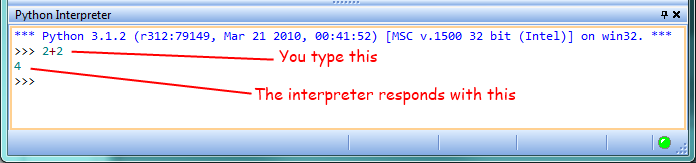
\includegraphics{interpreter_sshot.png}

The \code{\textgreater{}\textgreater{}\textgreater{}} is called the \textbf{Python prompt}. The interpreter uses the prompt to indicate that it is ready for
instructions. We typed \code{2 + 2}, and the interpreter evaluated our expression, and replied \code{4},
and on the next line it gave a new prompt, indicating that it is ready for more input.

Alternatively, you can write a program in a file and use the interpreter to
execute the contents of the file. Such a file is called a \textbf{script}.   Scripts have the
advantage that they can be saved to disk, printed, and so on.

In this Rhodes Local Edition of the textbook, we use a program development environment called
\textbf{PyScripter}. (It is available at \href{http://code.google.com/p/pyscripter}{http://code.google.com/p/pyscripter}.)  There are various other
development environments. If you're using one of the others, you might be
better off working with the authors' original book rather than this edition.

For example, we created a file named \code{firstprogram.py} using PyScripter.
By convention, files that contain Python programs have names that end with
\code{.py}

To execute the program, we can click the \textbf{Run} button in PyScripter:

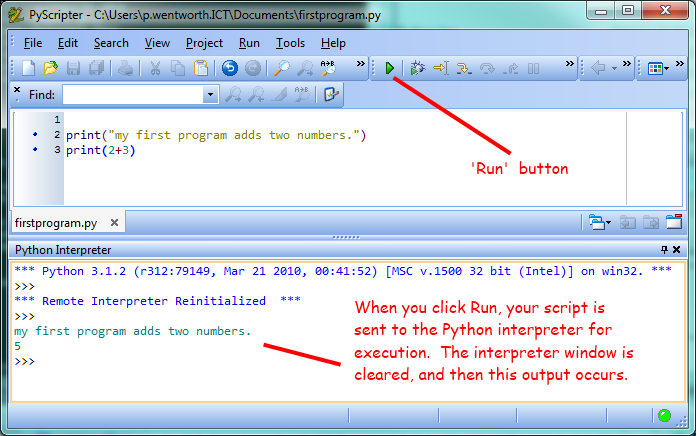
\includegraphics{my_first_program.png}

Most programs are more interesting than this one.

Working directly in the interpreter is convenient for testing short bits of code because you
get immediate feedback. Think of it as scratch paper used to help you work out
problems. Anything longer than a few lines should be put into a script.

\index{program}\index{algorithm}

\section{What is a program?}
\label{way_of_the_program:index-1}\label{way_of_the_program:what-is-a-program}
A \textbf{program} is a sequence of instructions that specifies how to perform a
computation. The computation might be something mathematical, such as solving a
system of equations or finding the roots of a polynomial, but it can also be a
symbolic computation, such as searching and replacing text in a document or
(strangely enough) compiling a program.

The details look different in different languages, but a few basic instructions
appear in just about every language:
\begin{description}
\item[{input}] \leavevmode
Get data from the keyboard, a file, or some other device.

\item[{output}] \leavevmode
Display data on the screen or send data to a file or other device.

\item[{math}] \leavevmode
Perform basic mathematical operations like addition and multiplication.

\item[{conditional execution}] \leavevmode
Check for certain conditions and execute the appropriate sequence of
statements.

\item[{repetition}] \leavevmode
Perform some action repeatedly, usually with some variation.

\end{description}

Believe it or not, that's pretty much all there is to it. Every program you've
ever used, no matter how complicated, is made up of instructions that look more
or less like these. Thus, we can describe programming as the process of
breaking a large, complex task into smaller and smaller subtasks until the
subtasks are simple enough to be performed with sequences of these basic
instructions.

That may be a little vague, but we will come back to this topic later when we
talk about \textbf{algorithms}.

\index{debugging}\index{bug}

\section{What is debugging?}
\label{way_of_the_program:what-is-debugging}\label{way_of_the_program:index-2}
Programming is a complex process, and because it is done by human beings, it
often leads to errors. Programming errors are called
\textbf{bugs} and the process of tracking them down and correcting them is called
\textbf{debugging}.  Use of the term \emph{bug} to describe small engineering difficulties
dates back to at least 1889, when Thomas Edison had a bug with his phonograph.

Three kinds of errors can occur in a program: \href{http://en.wikipedia.org/wiki/Syntax\_error}{syntax errors}, \href{http://en.wikipedia.org/wiki/Runtime\_error}{runtime errors}, and \href{http://en.wikipedia.org/wiki/Logic\_error}{semantic errors}.  It is useful to
distinguish between them in order to track them down more quickly.

\index{syntax}\index{syntax error}

\section{Syntax errors}
\label{way_of_the_program:syntax-errors}\label{way_of_the_program:index-3}
Python can only execute a program if the program is syntactically correct;
otherwise, the process fails and returns an error message.  \textbf{Syntax} refers
to the structure of a program and the rules about that structure. For example,
in English, a sentence must begin with a capital letter and end with a period.
this sentence contains a \textbf{syntax error}. So does this one

For most readers, a few syntax errors are not a significant problem, which is
why we can read the poetry of E. E. Cummings without problems.
Python is not so forgiving. If there is a single syntax error anywhere in your
program, Python will display an error message and quit, and you will not be able
to run your program. During the first few weeks of your programming career, you
will probably spend a lot of time tracking down syntax errors. As you gain
experience, though, you will make fewer errors and find them faster.

\index{runtime error}\index{exception}\index{safe language}

\section{Runtime errors}
\label{way_of_the_program:index-4}\label{way_of_the_program:runtime-errors}
The second type of error is a runtime error, so called because the error does
not appear until you run the program. These errors are also called
\textbf{exceptions} because they usually indicate that something exceptional (and
bad) has happened.

Runtime errors are rare in the simple programs you will see in the first few
chapters, so it might be a while before you encounter one.

\index{semantics}\index{semantic error}

\section{Semantic errors}
\label{way_of_the_program:index-5}\label{way_of_the_program:semantic-errors}
The third type of error is the \textbf{semantic error}. If there is a semantic error
in your program, it will run successfully, in the sense that the computer will
not generate any error messages, but it will not do the right thing. It will do
something else. Specifically, it will do what you told it to do.

The problem is that the program you wrote is not the program you wanted to
write. The meaning of the program (its semantics) is wrong.  Identifying
semantic errors can be tricky because it requires you to work backward by
looking at the output of the program and trying to figure out what it is doing.

\index{Holmes, Sherlock}\index{Doyle, Arthur Conan}\index{Linux}

\section{Experimental debugging}
\label{way_of_the_program:index-6}\label{way_of_the_program:experimental-debugging}
One of the most important skills you will acquire is debugging.  Although it
can be frustrating, debugging is one of the most intellectually rich,
challenging, and interesting parts of programming.

In some ways, debugging is like detective work. You are confronted with clues,
and you have to infer the processes and events that led to the results you see.

Debugging is also like an experimental science. Once you have an idea what is
going wrong, you modify your program and try again. If your hypothesis was
correct, then you can predict the result of the modification, and you take a
step closer to a working program. If your hypothesis was wrong, you have to
come up with a new one. As Sherlock Holmes pointed out, When you have
eliminated the impossible, whatever remains, however improbable, must be the
truth. (A. Conan Doyle, \emph{The Sign of Four})

For some people, programming and debugging are the same thing. That is,
programming is the process of gradually debugging a program until it does what
you want. The idea is that you should start with a program that does
\emph{something} and make small modifications, debugging them as you go, so that you
always have a working program.

For example, Linux is an operating system kernel that contains millions of
lines of code, but it started out as a simple program Linus Torvalds used to
explore the Intel 80386 chip. According to Larry Greenfield, one of Linus's
earlier projects was a program that would switch between displaying AAAA and
BBBB. This later evolved to Linux (\emph{The Linux Users' Guide} Beta Version 1).

Later chapters will make more suggestions about debugging and other programming
practices.

\index{formal language}\index{natural language}\index{parse}\index{token}

\section{Formal and natural languages}
\label{way_of_the_program:index-7}\label{way_of_the_program:formal-and-natural-languages}
\textbf{Natural languages} are the languages that people speak, such as English,
Spanish, and French. They were not designed by people (although people try to
impose some order on them); they evolved naturally.

\textbf{Formal languages} are languages that are designed by people for specific
applications. For example, the notation that mathematicians use is a formal
language that is particularly good at denoting relationships among numbers and
symbols. Chemists use a formal language to represent the chemical structure of
molecules. And most importantly:
\begin{quote}

\emph{Programming languages are formal languages that have been designed to
express computations.}
\end{quote}

Formal languages tend to have strict rules about syntax. For example, \code{3+3=6}
is a syntactically correct mathematical statement, but \code{3=+6\$} is not.
H$_{\text{2}}$O is a syntactically correct chemical name, but $_{\text{2}}$Zz is
not.

Syntax rules come in two flavors, pertaining to \textbf{tokens} and structure.
Tokens are the basic elements of the language, such as words, numbers, parentheses,
commas, and so on. In Python, a statement like \code{print("Happy New Year for ",2013)}
has 6 tokens: a function name, an open parenthesis (round bracket), a string, a comma, a number, and a close parenthesis.

It is possible to make errors in the way one constructs tokens.
One of the problems with \code{3=+6\$} is that \code{\$} is not a
legal token in mathematics (at least as far as we know). Similarly,
$_{\text{2}}$Zz is not a legal token in chemistry notation because there is no element with the abbreviation
\code{Zz}.

The second type of syntax rule pertains to the \textbf{structure} of a statement--- that
is, the way the tokens are arranged. The statement \code{3=+6\$} is structurally
illegal because you can't place a plus sign immediately after an equal sign.
Similarly, molecular formulas have to have subscripts after the element name,
not before.  And in our Python example, if we omitted the comma, or if we changed the two
parentheses around to say  \code{print)"Happy New Year for ",2013(} our statement would still
have six legal and valid tokens, but the structure is illegal.

When you read a sentence in English or a statement in a formal language, you
have to figure out what the structure of the sentence is (although in a natural
language you do this subconsciously). This process is called \textbf{parsing}.

For example, when you hear the sentence, ``The other shoe fell'', you understand
that the other shoe is the subject and fell is the verb.  Once you have parsed
a sentence, you can figure out what it means, or the \textbf{semantics} of the sentence.
Assuming that you know what a shoe is and what it means to fall, you will
understand the general implication of this sentence.

Although formal and natural languages have many features in common --- tokens,
structure, syntax, and semantics --- there are many differences:
\begin{description}
\item[{\index{ambiguity|textbf}ambiguity}] \leavevmode\phantomsection\label{way_of_the_program:term-ambiguity}
Natural languages are full of ambiguity, which people deal with by
using contextual clues and other information. Formal languages are
designed to be nearly or completely unambiguous, which means that any
statement has exactly one meaning, regardless of context.

\item[{\index{redundancy|textbf}redundancy}] \leavevmode\phantomsection\label{way_of_the_program:term-redundancy}
In order to make up for ambiguity and reduce misunderstandings, natural
languages employ lots of redundancy. As a result, they are often
verbose.  Formal languages are less redundant and more concise.

\item[{\index{literalness|textbf}literalness}] \leavevmode\phantomsection\label{way_of_the_program:term-literalness}
Formal languages mean exactly what they say.  On the other hand, natural languages
are full of idiom and metaphor. If someone says, ``The
other shoe fell'', there is probably no shoe and nothing falling.
You'll need to find the
original joke to understand the idiomatic meaning of the other shoe falling.
\emph{Yahoo! Answers} thinks it knows!

\end{description}

People who grow up speaking a natural language---everyone---often have a hard
time adjusting to formal languages. In some ways, the difference between formal
and natural language is like the difference between poetry and prose, but more
so:
\begin{description}
\item[{\index{poetry|textbf}poetry}] \leavevmode\phantomsection\label{way_of_the_program:term-poetry}
Words are used for their sounds as well as for their meaning, and the
whole poem together creates an effect or emotional response. Ambiguity
is not only common but often deliberate.

\item[{\index{prose|textbf}prose}] \leavevmode\phantomsection\label{way_of_the_program:term-prose}
The literal meaning of words is more important, and the structure
contributes more meaning. Prose is more amenable to analysis than
poetry but still often ambiguous.

\item[{\index{program|textbf}program}] \leavevmode\phantomsection\label{way_of_the_program:term-program}
The meaning of a computer program is unambiguous and literal, and can
be understood entirely by analysis of the tokens and structure.

\end{description}

Here are some suggestions for reading programs (and other formal languages).
First, remember that formal languages are much more dense than natural
languages, so it takes longer to read them. Also, the structure is very
important, so it is usually not a good idea to read from top to bottom, left to
right. Instead, learn to parse the program in your head, identifying the tokens
and interpreting the structure.  Finally, the details matter. Little things
like spelling errors and bad punctuation, which you can get away with in
natural languages, can make a big difference in a formal language.


\section{The first program}
\label{way_of_the_program:the-first-program}
Traditionally, the first program written in a new language is called \emph{Hello,
World!} because all it does is display the words, Hello, World!  In Python, the script
looks like this: (For scripts, we'll show line numbers to the left of the Python statements.)
\begin{quote}

\begin{Verbatim}[commandchars=\\\{\},numbers=left,firstnumber=1,stepnumber=1]
\PYG{n+nb}{print}\PYG{p}{(}\PYG{l+s}{"}\PYG{l+s}{Hello, World!}\PYG{l+s}{"}\PYG{p}{)}
\end{Verbatim}
\end{quote}

This is an example of using the \textbf{print function}, which doesn't actually print
anything on paper. It displays a value on the screen. In this case, the result shown
is
\begin{quote}

\begin{Verbatim}[commandchars=\\\{\}]
Hello, World!
\end{Verbatim}
\end{quote}

The quotation marks in the program mark the beginning and end of the value;
they don't appear in the result.

Some people judge the quality of a programming language by the simplicity of
the Hello, World! program. By this standard, Python does about as well as
possible.

\index{comment}

\section{Comments}
\label{way_of_the_program:index-8}\label{way_of_the_program:comments}
As programs get bigger and more complicated, they get more difficult to read.
Formal languages are dense, and it is often difficult to look at a piece of
code and figure out what it is doing, or why.

For this reason, it is a good idea to add notes to your programs to explain in
natural language what the program is doing.

A \textbf{comment} in a computer program is text that is intended
only for the human reader --- it is completely ignored by the interpreter.

In Python, the \emph{\#} token starts a comment.  The rest of the line
is ignored.   Here is a new version of \emph{Hello, World!}.
\begin{quote}

\begin{Verbatim}[commandchars=\\\{\},numbers=left,firstnumber=1,stepnumber=1]
\PYG{c}{\PYGZsh{}---------------------------------------------------}
\PYG{c}{\PYGZsh{} This demo program shows off how elegant Python is!}
\PYG{c}{\PYGZsh{} Written by Joe Soap, December 2010.}
\PYG{c}{\PYGZsh{} Anyone may freely copy or modify this program.}
\PYG{c}{\PYGZsh{}---------------------------------------------------}

\PYG{n+nb}{print}\PYG{p}{(}\PYG{l+s}{"}\PYG{l+s}{Hello, World!}\PYG{l+s}{"}\PYG{p}{)}     \PYG{c}{\PYGZsh{} Isn't this easy!}
\end{Verbatim}
\end{quote}

You'll also notice that we've left a blank line in the program.  Blank lines
are also ignored by the interpreter, but comments and blank lines can make your
programs much easier for humans to parse.  Use them liberally!


\section{Glossary}
\label{way_of_the_program:glossary}\begin{description}
\item[{\index{algorithm|textbf}algorithm}] \leavevmode\phantomsection\label{way_of_the_program:term-algorithm}
A set of specific steps for solving a category of problems.

\item[{\index{bug|textbf}bug}] \leavevmode\phantomsection\label{way_of_the_program:term-bug}
An error in a program.

\item[{\index{comment|textbf}comment}] \leavevmode\phantomsection\label{way_of_the_program:term-comment}
Information in a program that is meant for other programmers (or anyone
reading the source code) and has no effect on the execution of the
program.

\item[{\index{debugging|textbf}debugging}] \leavevmode\phantomsection\label{way_of_the_program:term-debugging}
The process of finding and removing any of the three kinds of
programming errors.

\item[{\index{exception|textbf}exception}] \leavevmode\phantomsection\label{way_of_the_program:term-exception}
Another name for a runtime error.

\item[{\index{formal language|textbf}formal language}] \leavevmode\phantomsection\label{way_of_the_program:term-formal-language}
Any one of the languages that people have designed for specific
purposes, such as representing mathematical ideas or computer programs;
all programming languages are formal languages.

\item[{\index{high-level language|textbf}high-level language}] \leavevmode\phantomsection\label{way_of_the_program:term-high-level-language}
A programming language like Python that is designed to be easy for
humans to read and write.

\item[{\index{immediate mode|textbf}immediate mode}] \leavevmode\phantomsection\label{way_of_the_program:term-immediate-mode}
A style of using Python where we type expressions at the command prompt, and
the results are shown immediately.  Contrast with \textbf{script}, and see the
entry under \textbf{Python shell}.

\item[{\index{interpreter|textbf}interpreter}] \leavevmode\phantomsection\label{way_of_the_program:term-interpreter}
The engine that executes your Python scripts or expressions.

\item[{\index{low-level language|textbf}low-level language}] \leavevmode\phantomsection\label{way_of_the_program:term-low-level-language}
A programming language that is designed to be easy for a computer to
execute; also called machine language or assembly language.

\item[{\index{natural language|textbf}natural language}] \leavevmode\phantomsection\label{way_of_the_program:term-natural-language}
Any one of the languages that people speak that evolved naturally.

\item[{\index{object code|textbf}object code}] \leavevmode\phantomsection\label{way_of_the_program:term-object-code}
The output of the compiler after it translates the program.

\item[{\index{parse|textbf}parse}] \leavevmode\phantomsection\label{way_of_the_program:term-parse}
To examine a program and analyze the syntactic structure.

\item[{\index{portability|textbf}portability}] \leavevmode\phantomsection\label{way_of_the_program:term-portability}
A property of a program that can run on more than one kind of computer.

\item[{\index{print function|textbf}print function}] \leavevmode\phantomsection\label{way_of_the_program:term-print-function}
A function used in a program or script that causes the Python interpreter to
display a value on its output device.

\item[{\index{problem solving|textbf}problem solving}] \leavevmode\phantomsection\label{way_of_the_program:term-problem-solving}
The process of formulating a problem, finding a solution, and
expressing the solution.

\item[{\index{program|textbf}program}] \leavevmode\phantomsection\label{way_of_the_program:term-22}
a sequence of instructions that specifies to a computer actions and
computations to be performed.

\item[{\index{Python shell|textbf}Python shell}] \leavevmode\phantomsection\label{way_of_the_program:term-python-shell}
An interactive user interface to the Python interpreter. The user of a
Python shell types commands at the prompt (\textgreater{}\textgreater{}\textgreater{}), and presses the return
key to send these commands immediately to the interpreter for
processing.  The word \emph{shell} comes from Unix.  In the PyScripter
used in this RLE version of the book, the Interpreter Window is where
we'd do the immediate mode interaction.

\item[{\index{runtime error|textbf}runtime error}] \leavevmode\phantomsection\label{way_of_the_program:term-runtime-error}
An error that does not occur until the program has started to execute
but that prevents the program from continuing.

\item[{\index{script|textbf}script}] \leavevmode\phantomsection\label{way_of_the_program:term-script}
A program stored in a file (usually one that will be interpreted).

\item[{\index{semantic error|textbf}semantic error}] \leavevmode\phantomsection\label{way_of_the_program:term-semantic-error}
An error in a program that makes it do something other than what the
programmer intended.

\item[{\index{semantics|textbf}semantics}] \leavevmode\phantomsection\label{way_of_the_program:term-semantics}
The meaning of a program.

\item[{\index{source code|textbf}source code}] \leavevmode\phantomsection\label{way_of_the_program:term-source-code}
A program in a high-level language before being compiled.

\item[{\index{syntax|textbf}syntax}] \leavevmode\phantomsection\label{way_of_the_program:term-syntax}
The structure of a program.

\item[{\index{syntax error|textbf}syntax error}] \leavevmode\phantomsection\label{way_of_the_program:term-syntax-error}
An error in a program that makes it impossible to parse --- and
therefore impossible to interpret.

\item[{\index{token|textbf}token}] \leavevmode\phantomsection\label{way_of_the_program:term-token}
One of the basic elements of the syntactic structure of a program,
analogous to a word in a natural language.

\end{description}


\section{Exercises}
\label{way_of_the_program:exercises}\begin{enumerate}
\item {} 
Write an English sentence with understandable semantics but incorrect
syntax. Write another English sentence which has correct syntax but has
semantic errors.

\item {} 
Using the Python interpreter, type \code{1 + 2} and then hit return. Python \emph{evaluates}
this \emph{expression}, displays the result, and then shows another prompt. \code{*}
is the \emph{multiplication operator}, and \code{**} is the
\emph{exponentiation operator}. Experiment by entering different expressions and
recording what is displayed by the Python interpreter.

\item {} 
Type \code{1 2} and then hit return. Python tries to evaluate the expression,
but it can't because the expression is not syntactically legal. Instead, it
shows the error message:
\begin{quote}

\begin{Verbatim}[commandchars=\\\{\}]
  \PYG{n}{File} \PYG{l+s}{"}\PYG{l+s}{\PYGZlt{}interactive input\PYGZgt{}}\PYG{l+s}{"}\PYG{p}{,} \PYG{n}{line} \PYG{l+m+mi}{1}
    \PYG{l+m+mi}{1} \PYG{l+m+mi}{2}
      \PYG{o}{\PYGZca{}}
\PYG{n+ne}{SyntaxError}\PYG{p}{:} \PYG{n}{invalid} \PYG{n}{syntax}
\end{Verbatim}
\end{quote}

In many cases, Python indicates where the syntax error occurred, but it is
not always right, and it doesn't give you much information about what is
wrong.

So, for the most part, the burden is on you to learn the syntax rules.

In this case, Python is complaining because there is no operator between the
numbers.

See if you can find a few more examples of things that will produce error
messages when you enter them at the Python prompt. Write down what you enter
at the prompt and the last line of the error message that Python reports
back to you.

\item {} 
Type  \code{print("hello")}. Python executes this, which has the effect
of printing the letters h-e-l-l-o. Notice that the quotation marks that you
used to enclose the string are not part of the output.  Now type \code{"hello"}
and describe your result.  Make notes of when you see the quotation marks
and when you don't.

\item {} 
Type \code{cheese} without the quotation marks. The output will look
something like this:

\begin{Verbatim}[commandchars=\\\{\}]
Traceback (most recent call last):
  File "\textless{}interactive input\textgreater{}", line 1, in ?
NameError: name 'cheese' is not defined
\end{Verbatim}

This is a run-time error; specifically, it is a NameError, and even more
specifically, it is an error because the name \emph{cheese} is not defined. If
you don't know what that means yet, you will soon.

\item {} 
Type \code{6 + 4 * 9} at the Python prompt and hit enter.  Record what
happens.

Now create a Python script with the following contents:
\begin{quote}

\begin{Verbatim}[commandchars=\\\{\},numbers=left,firstnumber=1,stepnumber=1]
 \PYG{l+m+mi}{6} \PYG{o}{+} \PYG{l+m+mi}{4} \PYG{o}{*} \PYG{l+m+mi}{9}
\end{Verbatim}
\end{quote}

What happens when you run this script? Now change the script contents to:
\begin{quote}

\begin{Verbatim}[commandchars=\\\{\},numbers=left,firstnumber=1,stepnumber=1]
\PYG{n+nb}{print}\PYG{p}{(}\PYG{l+m+mi}{6} \PYG{o}{+} \PYG{l+m+mi}{4} \PYG{o}{*} \PYG{l+m+mi}{9}\PYG{p}{)}
\end{Verbatim}
\end{quote}

and run it again.

What happened this time?

Whenever an \emph{expression} is typed at the Python prompt, it is evaluated
and the result is \emph{automatically} shown on the line below.  (Like on your calculator,
if you type this expression you'll get the result 42.)

A script is different, however.  Evaluations of
expressions are not automatically displayed,
so it is necessary to use the \textbf{print} function to make the answer
show up.

It is hardly ever necessary to use the print function in immediate mode at the command prompt.

\end{enumerate}

\begin{DUlineblock}{0em}
\item[] 
\end{DUlineblock}


\chapter{Variables, expressions and statements}
\label{variables_expressions_statements:variables-expressions-and-statements}\label{variables_expressions_statements::doc}
\index{value}\index{data type}\index{string}\index{integer}\index{int}\index{float}\index{class}\index{type}
\index{triple quoted string}

\section{Values and data types}
\label{variables_expressions_statements:values-n-types}\label{variables_expressions_statements:values-and-data-types}\label{variables_expressions_statements:index-1}
A \textbf{value} is one of the fundamental things --- like a letter or a number ---
that a program manipulates. The values we have seen so far are \code{4} (the
result when we added \code{2 + 2}), and \code{"Hello, World!"}.

These values are classified into different \textbf{classes}, or \textbf{data types}: \code{4}
is an \emph{integer}, and \code{"Hello, World!"} is a \emph{string},
so-called because it contains a string of
letters. You (and the interpreter) can identify strings because they are
enclosed in quotation marks.

If you are not sure what class a value falls into, Python has a function
called \textbf{type} which can tell you.
\begin{quote}

\begin{Verbatim}[commandchars=\\\{\}]
\PYG{g+gp}{\PYGZgt{}\PYGZgt{}\PYGZgt{} }\PYG{n+nb}{type}\PYG{p}{(}\PYG{l+s}{"}\PYG{l+s}{Hello, World!}\PYG{l+s}{"}\PYG{p}{)}
\PYG{g+go}{\PYGZlt{}class 'str'\PYGZgt{}}
\PYG{g+gp}{\PYGZgt{}\PYGZgt{}\PYGZgt{} }\PYG{n+nb}{type}\PYG{p}{(}\PYG{l+m+mi}{17}\PYG{p}{)}
\PYG{g+go}{\PYGZlt{}class 'int'\PYGZgt{}}
\end{Verbatim}
\end{quote}

Not surprisingly, strings belong to the class \textbf{str} and integers belong to the
class \textbf{int}. Less obviously, numbers with a decimal point belong to a class
called \textbf{float}, because these numbers are represented in a format called
\emph{floating-point}.  At this stage, you can treat the words \emph{class} and \emph{type}
interchangeably.  We'll come back to a deeper understanding of what a class
is in later chapters.
\begin{quote}

\begin{Verbatim}[commandchars=\\\{\}]
\PYG{g+gp}{\PYGZgt{}\PYGZgt{}\PYGZgt{} }\PYG{n+nb}{type}\PYG{p}{(}\PYG{l+m+mf}{3.2}\PYG{p}{)}
\PYG{g+go}{\PYGZlt{}class 'float'\PYGZgt{}}
\end{Verbatim}
\end{quote}

What about values like \code{"17"} and \code{"3.2"}? They look like numbers, but they
are in quotation marks like strings.
\begin{quote}

\begin{Verbatim}[commandchars=\\\{\}]
\PYG{g+gp}{\PYGZgt{}\PYGZgt{}\PYGZgt{} }\PYG{n+nb}{type}\PYG{p}{(}\PYG{l+s}{"}\PYG{l+s}{17}\PYG{l+s}{"}\PYG{p}{)}
\PYG{g+go}{\PYGZlt{}class 'str'\PYGZgt{}}
\PYG{g+gp}{\PYGZgt{}\PYGZgt{}\PYGZgt{} }\PYG{n+nb}{type}\PYG{p}{(}\PYG{l+s}{"}\PYG{l+s}{3.2}\PYG{l+s}{"}\PYG{p}{)}
\PYG{g+go}{\PYGZlt{}class 'str'\PYGZgt{}}
\end{Verbatim}
\end{quote}

They're strings!

Strings in Python can be enclosed in either single quotes (\code{'}) or double quotes
(\code{"}), or three of each (\code{'''} or \code{"""})
\begin{quote}

\begin{Verbatim}[commandchars=\\\{\}]
\PYG{g+gp}{\PYGZgt{}\PYGZgt{}\PYGZgt{} }\PYG{n+nb}{type}\PYG{p}{(}\PYG{l+s}{'}\PYG{l+s}{This is a string.}\PYG{l+s}{'}\PYG{p}{)}
\PYG{g+go}{\PYGZlt{}class 'str'\PYGZgt{}}
\PYG{g+gp}{\PYGZgt{}\PYGZgt{}\PYGZgt{} }\PYG{n+nb}{type}\PYG{p}{(}\PYG{l+s}{"}\PYG{l+s}{And so is this.}\PYG{l+s}{"}\PYG{p}{)}
\PYG{g+go}{\PYGZlt{}class 'str'\PYGZgt{}}
\PYG{g+gp}{\PYGZgt{}\PYGZgt{}\PYGZgt{} }\PYG{n+nb}{type}\PYG{p}{(}\PYG{l+s}{"""}\PYG{l+s}{and this.}\PYG{l+s}{"""}\PYG{p}{)}
\PYG{g+go}{\PYGZlt{}class 'str'\PYGZgt{}}
\PYG{g+gp}{\PYGZgt{}\PYGZgt{}\PYGZgt{} }\PYG{n+nb}{type}\PYG{p}{(}\PYG{l+s}{'''}\PYG{l+s}{and even this...}\PYG{l+s}{'''}\PYG{p}{)}
\PYG{g+go}{\PYGZlt{}class 'str'\PYGZgt{}}
\end{Verbatim}
\end{quote}

Double quoted strings can contain single quotes inside them, as in
\code{"Bruce's beard"}, and single quoted strings can have double quotes
inside them, as in \code{'The knights who say "Ni!"'}.

Strings enclosed with three occurrences of either quote symbol are
called triple quoted strings.  They can
contain either single or double quotes:
\begin{quote}

\begin{Verbatim}[commandchars=\\\{\}]
\PYG{g+gp}{\PYGZgt{}\PYGZgt{}\PYGZgt{} }\PYG{n+nb}{print}\PYG{p}{(}\PYG{l+s}{'''}\PYG{l+s}{"}\PYG{l+s}{Oh no}\PYG{l+s}{"}\PYG{l+s}{, she exclaimed, }\PYG{l+s}{"}\PYG{l+s}{Ben}\PYG{l+s}{'}\PYG{l+s}{s bike is broken!}\PYG{l+s}{"}\PYG{l+s}{'''}\PYG{p}{)}
\PYG{g+go}{"Oh no", she exclaimed, "Ben's bike is broken!"}
\PYG{g+go}{\PYGZgt{}\PYGZgt{}\PYGZgt{}}
\end{Verbatim}
\end{quote}

Triple quoted strings can even span multiple lines:
\begin{quote}

\begin{Verbatim}[commandchars=\\\{\}]
\PYG{g+gp}{\PYGZgt{}\PYGZgt{}\PYGZgt{} }\PYG{n}{message} \PYG{o}{=} \PYG{l+s}{"""}\PYG{l+s}{This message will}
\PYG{g+gp}{... }\PYG{l+s}{span several}
\PYG{g+gp}{... }\PYG{l+s}{lines.}\PYG{l+s}{"""}
\PYG{g+gp}{\PYGZgt{}\PYGZgt{}\PYGZgt{} }\PYG{n+nb}{print}\PYG{p}{(}\PYG{n}{message}\PYG{p}{)}
\PYG{g+go}{This message will}
\PYG{g+go}{span several}
\PYG{g+go}{lines.}
\PYG{g+go}{\PYGZgt{}\PYGZgt{}\PYGZgt{}}
\end{Verbatim}
\end{quote}

Python doesn't care whether you use single or double quotes or
the three-of-a-kind quotes to surround your strings:
once it has parsed the text of your program or command, the way it stores the
value is identical in all cases, and the surrounding quotes are not part of
the value. But when the interpreter wants to display a string, it has to
decide which quotes to use to make it look like a string.
\begin{quote}

\begin{Verbatim}[commandchars=\\\{\}]
\PYG{g+gp}{\PYGZgt{}\PYGZgt{}\PYGZgt{} }\PYG{l+s}{'}\PYG{l+s}{This is a string.}\PYG{l+s}{'}
\PYG{g+go}{'This is a string.'}
\PYG{g+gp}{\PYGZgt{}\PYGZgt{}\PYGZgt{} }\PYG{l+s+sd}{"""And so is this."""}
\PYG{g+go}{'And so is this.'}
\end{Verbatim}
\end{quote}

So the Python language designers usually chose to surround their strings
by single quotes.  What do think would happen if the string already
contained single quotes?

When you type a large integer, you might be tempted to use commas between
groups of three digits, as in \code{42,000}. This is not a legal integer in
Python, but it does mean something else, which is legal:
\begin{quote}

\begin{Verbatim}[commandchars=\\\{\}]
\PYG{g+gp}{\PYGZgt{}\PYGZgt{}\PYGZgt{} }\PYG{l+m+mi}{42000}
\PYG{g+go}{42000}
\PYG{g+gp}{\PYGZgt{}\PYGZgt{}\PYGZgt{} }\PYG{l+m+mi}{42}\PYG{p}{,}\PYG{l+m+mi}{000}
\PYG{g+go}{(42, 0)}
\end{Verbatim}
\end{quote}

Well, that's not what we expected at all! Because of the comma, Python chose to
treat this as a \emph{pair} of values.  We'll come back to learn about pairs later.
But, for the moment, remember not to put commas or spaces in your integers, no matter
how big they are. Also revisit what we said in the previous chapter: formal languages are
strict, the notation is concise, and even the smallest change might
mean something quite different from what you intended.

\index{variable}\index{assignment}\index{assignment statement}\index{state snapshot}

\section{Variables}
\label{variables_expressions_statements:variables}\label{variables_expressions_statements:index-2}
One of the most powerful features of a programming language is the ability to
manipulate \textbf{variables}. A variable is a name that refers to a value.

The \textbf{assignment statement} gives a value to a variable:
\begin{quote}

\begin{Verbatim}[commandchars=\\\{\}]
\PYG{g+gp}{\PYGZgt{}\PYGZgt{}\PYGZgt{} }\PYG{n}{message} \PYG{o}{=} \PYG{l+s}{"}\PYG{l+s}{What}\PYG{l+s}{'}\PYG{l+s}{s up, Doc?}\PYG{l+s}{"}
\PYG{g+gp}{\PYGZgt{}\PYGZgt{}\PYGZgt{} }\PYG{n}{n} \PYG{o}{=} \PYG{l+m+mi}{17}
\PYG{g+gp}{\PYGZgt{}\PYGZgt{}\PYGZgt{} }\PYG{n}{pi} \PYG{o}{=} \PYG{l+m+mf}{3.14159}
\end{Verbatim}
\end{quote}

This example makes three assignments. The first assigns the string value \code{"What's
up, Doc?"} to a variable named \code{message}. The second gives the integer
\code{17} to \code{n}, and the third assigns the floating-point number \code{3.14159} to
a variable called \code{pi}.

The \textbf{assignment token}, \code{=}, should not be confused with \emph{equals}, which uses
the token \code{==}.  The assignment statement binds a \emph{name}, on the
left-hand side of the operator, to a \emph{value}, on the right-hand side.
This is why you will get an error if you enter:
\begin{quote}

\begin{Verbatim}[commandchars=\\\{\}]
\PYG{g+gp}{\PYGZgt{}\PYGZgt{}\PYGZgt{} }\PYG{l+m+mi}{17} \PYG{o}{=} \PYG{n}{n}
\PYG{g+go}{File "\PYGZlt{}interactive input\PYGZgt{}", line 1}
\PYG{g+go}{SyntaxError: can't assign to literal}
\end{Verbatim}

\begin{notice}{tip}{Tip:}
When reading or writing code, say to yourself ``n is assigned 17''
or ``n gets the value 17''.  Don't say ``n equals 17''.
\end{notice}
\end{quote}

A common way to represent variables on paper is to write the name with an arrow
pointing to the variable's value. This kind of figure is called a \textbf{state
snapshot} because it shows what state each of the variables is in at a particular
instant in time.  (Think of it as the variable's state of mind).
This diagram shows the result of executing the assignment statements:
\begin{quote}

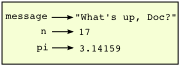
\includegraphics{state.png}
\end{quote}

If you ask the interpreter to evaluate a variable, it will produce the value that is currently
linked to the variable:
\begin{quote}

\begin{Verbatim}[commandchars=\\\{\}]
\PYG{g+gp}{\PYGZgt{}\PYGZgt{}\PYGZgt{} }\PYG{n}{message}
\PYG{g+go}{'What's up, Doc?'}
\PYG{g+gp}{\PYGZgt{}\PYGZgt{}\PYGZgt{} }\PYG{n}{n}
\PYG{g+go}{17}
\PYG{g+gp}{\PYGZgt{}\PYGZgt{}\PYGZgt{} }\PYG{n}{pi}
\PYG{g+go}{3.14159}
\end{Verbatim}
\end{quote}

We use variables in a program to ``remember'' things, perhaps the current score at the football game.
But variables are \emph{variable}. This means they can change over time, just like the scoreboard at a football game.
You can assign a value to a variable, and later assign a different value to the same variable.
(\emph{This is different from maths. In maths, if you give {}`x{}` the value 3, it
cannot change to link to a different value half-way through your calculations!})
\begin{quote}

\begin{Verbatim}[commandchars=\\\{\}]
\PYG{g+gp}{\PYGZgt{}\PYGZgt{}\PYGZgt{} }\PYG{n}{day} \PYG{o}{=} \PYG{l+s}{"}\PYG{l+s}{Thursday}\PYG{l+s}{"}
\PYG{g+gp}{\PYGZgt{}\PYGZgt{}\PYGZgt{} }\PYG{n}{day}
\PYG{g+go}{'Thursday'}
\PYG{g+gp}{\PYGZgt{}\PYGZgt{}\PYGZgt{} }\PYG{n}{day} \PYG{o}{=} \PYG{l+s}{"}\PYG{l+s}{Friday}\PYG{l+s}{"}
\PYG{g+gp}{\PYGZgt{}\PYGZgt{}\PYGZgt{} }\PYG{n}{day}
\PYG{g+go}{'Friday'}
\PYG{g+gp}{\PYGZgt{}\PYGZgt{}\PYGZgt{} }\PYG{n}{day} \PYG{o}{=} \PYG{l+m+mi}{21}
\PYG{g+gp}{\PYGZgt{}\PYGZgt{}\PYGZgt{} }\PYG{n}{day}
\PYG{g+go}{21}
\end{Verbatim}
\end{quote}

You'll notice we changed the value of \code{day} three times, and on the third assignment we even
made it refer to a value that was of a different type.

A great deal of programming is about having the computer remember things, e.g. \emph{The number of missed calls on your phone},
and then arranging to update or change the variable when you miss another call.

\index{keyword}\index{underscore character}

\section{Variable names and keywords}
\label{variables_expressions_statements:variable-names-and-keywords}\label{variables_expressions_statements:index-3}
\textbf{Variable names} can be arbitrarily long. They can contain both letters and
digits, but they have to begin with a letter or an underscore. Although it is legal to use
uppercase letters, by convention we don't. If you do, remember that case
matters. \code{Bruce} and \code{bruce} are different variables.

The underscore character ( \code{\_}) can appear in a name. It is often used in
names with multiple words, such as \code{my\_name} or \code{price\_of\_tea\_in\_china}.

There are some situations in which names beginning with an underscore have
special meaning, so a safe rule for beginners is to start all names with a letter.

If you give a variable an illegal name, you get a syntax error:
\begin{quote}

\begin{Verbatim}[commandchars=\\\{\}]
\textgreater{}\textgreater{}\textgreater{} 76trombones = "big parade"
SyntaxError: invalid syntax
\textgreater{}\textgreater{}\textgreater{} more\$ = 1000000
SyntaxError: invalid syntax
\textgreater{}\textgreater{}\textgreater{} class = "Computer Science 101"
SyntaxError: invalid syntax
\end{Verbatim}
\end{quote}

\code{76trombones} is illegal because it does not begin with a letter.  \code{more\$}
is illegal because it contains an illegal character, the dollar sign. But
what's wrong with \code{class}?

It turns out that \code{class} is one of the Python \textbf{keywords}. Keywords define
the language's syntax rules and structure, and they cannot be used as variable names.

Python has thirty-something keywords (and every now and again improvements to Python
introduce or eliminate one or two):

\begin{tabulary}{\linewidth}{|L|L|L|L|L|L|}
\hline

and
 & 
as
 & 
assert
 & 
break
 & 
class
 & 
continue
\\\hline

def
 & 
del
 & 
elif
 & 
else
 & 
except
 & 
exec
\\\hline

finally
 & 
for
 & 
from
 & 
global
 & 
if
 & 
import
\\\hline

in
 & 
is
 & 
lambda
 & 
nonlocal
 & 
not
 & 
or
\\\hline

pass
 & 
raise
 & 
return
 & 
try
 & 
while
 & 
with
\\\hline

yield
 & 
True
 & 
False
 & 
None
 &  & \\\hline
\end{tabulary}


You might want to keep this list handy. If the interpreter complains about one
of your variable names and you don't know why, see if it is on this list.

Programmers generally choose names for their variables that are meaningful to
the human readers of the program ---
they help the programmer document, or remember, what the variable is used for.

\begin{notice}{caution}{Caution:}
Beginners sometimes confuse ``meaningful to the human readers'' with ``meaningful to the computer''.
So they'll wrongly think that because they've called some variable \code{average} or \code{pi}, it will
somehow magically calculate an average, or magically know that the variable \code{pi} should have a
value like 3.14159.  No! The computer doesn't understand what you intend the variable to mean.

So you'll find some instructors who deliberately don't choose meaningful
names when they teach beginners --- not because we don't think it is a good habit,
but because we're trying to reinforce the message that you --- the programmer --- must
write the program code to calculate the average, and you must write an assignment
statement to give the variable \code{pi} the value you want it to have.
\end{notice}

\index{statement}

\section{Statements}
\label{variables_expressions_statements:index-4}\label{variables_expressions_statements:statements}
A \textbf{statement} is an instruction that the Python interpreter can execute. We
have only seen the assignment statement so far.  Some other kinds of statements that
we'll see shortly are \code{while} statements, \code{for} statements, \code{if} statements,
and \code{import} statements.  (There are other kinds too!)

When you type a statement on the command line, Python executes it.  Statements
don't produce any result.

\index{expression}

\section{Evaluating expressions}
\label{variables_expressions_statements:evaluating-expressions}\label{variables_expressions_statements:index-5}
An \textbf{expression} is a combination of values, variables, operators, and calls to functions. If you
type an expression at the Python prompt, the interpreter \textbf{evaluates} it and
displays the result:
\begin{quote}

\begin{Verbatim}[commandchars=\\\{\}]
\PYG{g+gp}{\PYGZgt{}\PYGZgt{}\PYGZgt{} }\PYG{l+m+mi}{1} \PYG{o}{+} \PYG{l+m+mi}{1}
\PYG{g+go}{2}
\PYG{g+gp}{\PYGZgt{}\PYGZgt{}\PYGZgt{} }\PYG{n+nb}{len}\PYG{p}{(}\PYG{l+s}{"}\PYG{l+s}{hello}\PYG{l+s}{"}\PYG{p}{)}
\PYG{g+go}{5}
\end{Verbatim}
\end{quote}

In this example \code{len} is a built-in Python function that returns the number of characters in a string.
We've previously seen the \code{print} and the \code{type} functions, so this is our third example of a function!

The \emph{evaluation of an expression} produces a value, which is why expressions
can appear on the right hand side of assignment statements. A value all by
itself is a simple expression, and so is a variable.
\begin{quote}

\begin{Verbatim}[commandchars=\\\{\}]
\PYG{g+gp}{\PYGZgt{}\PYGZgt{}\PYGZgt{} }\PYG{l+m+mi}{17}
\PYG{g+go}{17}
\PYG{g+gp}{\PYGZgt{}\PYGZgt{}\PYGZgt{} }\PYG{n}{y} \PYG{o}{=} \PYG{l+m+mf}{3.14}
\PYG{g+gp}{\PYGZgt{}\PYGZgt{}\PYGZgt{} }\PYG{n}{x} \PYG{o}{=} \PYG{n+nb}{len}\PYG{p}{(}\PYG{l+s}{"}\PYG{l+s}{hello}\PYG{l+s}{"}\PYG{p}{)}
\PYG{g+gp}{\PYGZgt{}\PYGZgt{}\PYGZgt{} }\PYG{n}{x}
\PYG{g+go}{5}
\PYG{g+gp}{\PYGZgt{}\PYGZgt{}\PYGZgt{} }\PYG{n}{y}
\PYG{g+go}{3.14}
\end{Verbatim}
\end{quote}

\index{operator}\index{operand}\index{floor division}

\section{Operators and operands}
\label{variables_expressions_statements:operators-and-operands}\label{variables_expressions_statements:index-6}
\textbf{Operators} are special tokens that represent computations like addition,
multiplication and division. The values the operator uses are called \textbf{operands}.

The following are all legal Python expressions whose meaning is more or less
clear:

\begin{Verbatim}[commandchars=\\\{\}]
20+32   hour-1   hour*60+minute   minute/60   5**2   (5+9)*(15-7)
\end{Verbatim}

The tokens \code{+}, \code{-}, and \code{*}, and the use of parenthesis for grouping,
mean in Python what they mean in mathematics. The asterisk (\code{*}) is the
token for multiplication, and \code{**} is the token for exponentiation.
\begin{quote}

\begin{Verbatim}[commandchars=\\\{\}]
\PYG{g+gp}{\PYGZgt{}\PYGZgt{}\PYGZgt{} }\PYG{l+m+mi}{2} \PYG{o}{*}\PYG{o}{*} \PYG{l+m+mi}{3}
\PYG{g+go}{8}
\PYG{g+gp}{\PYGZgt{}\PYGZgt{}\PYGZgt{} }\PYG{l+m+mi}{3} \PYG{o}{*}\PYG{o}{*} \PYG{l+m+mi}{2}
\PYG{g+go}{9}
\end{Verbatim}
\end{quote}

When a variable name appears in the place of an operand, it is replaced with
its value before the operation is performed.

Addition, subtraction, multiplication, and exponentiation all do what you
expect.

Example: so let us convert 645 minutes into hours:
\begin{quote}

\begin{Verbatim}[commandchars=\\\{\}]
\PYG{g+gp}{\PYGZgt{}\PYGZgt{}\PYGZgt{} }\PYG{n}{minutes} \PYG{o}{=} \PYG{l+m+mi}{645}
\PYG{g+gp}{\PYGZgt{}\PYGZgt{}\PYGZgt{} }\PYG{n}{hours} \PYG{o}{=} \PYG{n}{minutes} \PYG{o}{/} \PYG{l+m+mi}{60}
\PYG{g+gp}{\PYGZgt{}\PYGZgt{}\PYGZgt{} }\PYG{n}{hours}
\PYG{g+go}{10.75}
\end{Verbatim}
\end{quote}

Oops! In Python 3, the division operator \code{/} always yields a floating point result.
What we might have wanted to know was how many \emph{whole} hours there are, and how many minutes remain.
Python gives us two different flavors of the division operator.
The second, called \textbf{floor division} uses the token \emph{//}.
Its result is always a whole number --- and if it has to adjust the number it always
moves it to the left on the number line.  So \emph{6 // 4} yields \emph{1}, but \emph{-6 // 4} might surprise you!
\begin{quote}

\begin{Verbatim}[commandchars=\\\{\}]
\PYG{g+gp}{\PYGZgt{}\PYGZgt{}\PYGZgt{} }\PYG{l+m+mi}{7} \PYG{o}{/} \PYG{l+m+mi}{4}
\PYG{g+go}{1.75}
\PYG{g+gp}{\PYGZgt{}\PYGZgt{}\PYGZgt{} }\PYG{l+m+mi}{7} \PYG{o}{/}\PYG{o}{/} \PYG{l+m+mi}{4}
\PYG{g+go}{1}
\PYG{g+gp}{\PYGZgt{}\PYGZgt{}\PYGZgt{} }\PYG{n}{minutes} \PYG{o}{=} \PYG{l+m+mi}{645}
\PYG{g+gp}{\PYGZgt{}\PYGZgt{}\PYGZgt{} }\PYG{n}{hours} \PYG{o}{=} \PYG{n}{minutes} \PYG{o}{/}\PYG{o}{/} \PYG{l+m+mi}{60}
\PYG{g+gp}{\PYGZgt{}\PYGZgt{}\PYGZgt{} }\PYG{n}{hours}
\PYG{g+go}{10}
\end{Verbatim}
\end{quote}

Take care that you choose the correct flavor of the division operator.  If you're
working with expressions where you need floating point values, use the division operator
that does the division accurately.

\index{type converter functions}\index{int}\index{float}\index{str}\index{truncation}

\section{Type converter functions}
\label{variables_expressions_statements:index-7}\label{variables_expressions_statements:type-converter-functions}
Here we'll look at three more Python functions, \code{int}, \code{float} and \code{str}, which will (attempt to)
convert their arguments into types \code{int}, \code{float} and \code{str} respectively.  We call these
\textbf{type converter} functions.

The \code{int} function can take a floating point number or a string, and turn
it into an int. For floating point numbers, it \emph{discards} the decimal portion
of the number --- a process we call \emph{truncation towards zero} on
the number line.  Let us see this in action:
\begin{quote}

\begin{Verbatim}[commandchars=\\\{\}]
\PYG{g+gp}{\PYGZgt{}\PYGZgt{}\PYGZgt{} }\PYG{n+nb}{int}\PYG{p}{(}\PYG{l+m+mf}{3.14}\PYG{p}{)}
\PYG{g+go}{3}
\PYG{g+gp}{\PYGZgt{}\PYGZgt{}\PYGZgt{} }\PYG{n+nb}{int}\PYG{p}{(}\PYG{l+m+mf}{3.9999}\PYG{p}{)}             \PYG{c}{\PYGZsh{} This doesn't round to the closest int!}
\PYG{g+go}{3}
\PYG{g+gp}{\PYGZgt{}\PYGZgt{}\PYGZgt{} }\PYG{n+nb}{int}\PYG{p}{(}\PYG{l+m+mf}{3.0}\PYG{p}{)}
\PYG{g+go}{3}
\PYG{g+gp}{\PYGZgt{}\PYGZgt{}\PYGZgt{} }\PYG{n+nb}{int}\PYG{p}{(}\PYG{o}{-}\PYG{l+m+mf}{3.999}\PYG{p}{)}             \PYG{c}{\PYGZsh{} Note that the result is closer to zero}
\PYG{g+go}{-3}
\PYG{g+gp}{\PYGZgt{}\PYGZgt{}\PYGZgt{} }\PYG{n+nb}{int}\PYG{p}{(}\PYG{n}{minutes} \PYG{o}{/} \PYG{l+m+mi}{60}\PYG{p}{)}
\PYG{g+go}{10}
\PYG{g+gp}{\PYGZgt{}\PYGZgt{}\PYGZgt{} }\PYG{n+nb}{int}\PYG{p}{(}\PYG{l+s}{"}\PYG{l+s}{2345}\PYG{l+s}{"}\PYG{p}{)}             \PYG{c}{\PYGZsh{} Parse a string to produce an int}
\PYG{g+go}{2345}
\PYG{g+gp}{\PYGZgt{}\PYGZgt{}\PYGZgt{} }\PYG{n+nb}{int}\PYG{p}{(}\PYG{l+m+mi}{17}\PYG{p}{)}                 \PYG{c}{\PYGZsh{} It even works if arg is already an int}
\PYG{g+go}{17}
\PYG{g+gp}{\PYGZgt{}\PYGZgt{}\PYGZgt{} }\PYG{n+nb}{int}\PYG{p}{(}\PYG{l+s}{"}\PYG{l+s}{23 bottles}\PYG{l+s}{"}\PYG{p}{)}
\end{Verbatim}
\end{quote}

This last case doesn't look like a number --- what do we expect?
\begin{quote}

\begin{Verbatim}[commandchars=\\\{\}]
\PYG{n}{Traceback} \PYG{p}{(}\PYG{n}{most} \PYG{n}{recent} \PYG{n}{call} \PYG{n}{last}\PYG{p}{)}\PYG{p}{:}
\PYG{n}{File} \PYG{l+s}{"}\PYG{l+s}{\PYGZlt{}interactive input\PYGZgt{}}\PYG{l+s}{"}\PYG{p}{,} \PYG{n}{line} \PYG{l+m+mi}{1}\PYG{p}{,} \PYG{o+ow}{in} \PYG{o}{\PYGZlt{}}\PYG{n}{module}\PYG{o}{\PYGZgt{}}
\PYG{n+ne}{ValueError}\PYG{p}{:} \PYG{n}{invalid} \PYG{n}{literal} \PYG{k}{for} \PYG{n+nb}{int}\PYG{p}{(}\PYG{p}{)} \PYG{k}{with} \PYG{n}{base} \PYG{l+m+mi}{10}\PYG{p}{:} \PYG{l+s}{'}\PYG{l+s}{23 bottles}\PYG{l+s}{'}
\end{Verbatim}
\end{quote}

The type converter \code{float} can turn an integer, a float, or a syntactically legal
string into a float:
\begin{quote}

\begin{Verbatim}[commandchars=\\\{\}]
\PYG{g+gp}{\PYGZgt{}\PYGZgt{}\PYGZgt{} }\PYG{n+nb}{float}\PYG{p}{(}\PYG{l+m+mi}{17}\PYG{p}{)}
\PYG{g+go}{17.0}
\PYG{g+gp}{\PYGZgt{}\PYGZgt{}\PYGZgt{} }\PYG{n+nb}{float}\PYG{p}{(}\PYG{l+s}{"}\PYG{l+s}{123.45}\PYG{l+s}{"}\PYG{p}{)}
\PYG{g+go}{123.45}
\end{Verbatim}
\end{quote}

The type converter \code{str} turns its argument into a string:
\begin{quote}

\begin{Verbatim}[commandchars=\\\{\}]
\PYG{g+gp}{\PYGZgt{}\PYGZgt{}\PYGZgt{} }\PYG{n+nb}{str}\PYG{p}{(}\PYG{l+m+mi}{17}\PYG{p}{)}
\PYG{g+go}{'17'}
\PYG{g+gp}{\PYGZgt{}\PYGZgt{}\PYGZgt{} }\PYG{n+nb}{str}\PYG{p}{(}\PYG{l+m+mf}{123.45}\PYG{p}{)}
\PYG{g+go}{'123.45'}
\end{Verbatim}
\end{quote}

\index{order of operations}\index{rules of precedence}

\section{Order of operations}
\label{variables_expressions_statements:index-8}\label{variables_expressions_statements:order-of-operations}
When more than one operator appears in an expression, the order of evaluation
depends on the \textbf{rules of precedence}. Python follows the same precedence
rules for its mathematical operators that mathematics does. The acronym PEMDAS
is a useful way to remember the order of operations:
\begin{enumerate}
\item {} 
\textbf{P}arentheses have the highest precedence and can be used to force an
expression to evaluate in the order you want. Since expressions in
parentheses are evaluated first, \code{2 * (3-1)} is 4, and \code{(1+1)**(5-2)} is
8. You can also use parentheses to make an expression easier to read, as in
\code{(minute * 100) / 60}, even though it doesn't change the result.

\item {} 
\textbf{E}xponentiation has the next highest precedence, so \code{2**1+1} is 3 and
not 4, and \code{3*1**3} is 3 and not 27.

\item {} 
\textbf{M}ultiplication and both \textbf{D}ivision operators have the same precedence, which is
higher than \textbf{A}ddition and \textbf{S}ubtraction, which also have the same
precedence. So \code{2*3-1} yields 5 rather than 4, and \code{5-2*2} is 1, not 6.

\item {} 
Operators with the \emph{same} precedence are evaluated from left-to-right. In algebra
we say they are \emph{left-associative}.  So in
the expression \code{6-3+2}, the subtraction happens first, yielding 3. We then add
2 to get the result 5. If the operations had been evaluated from
right to left, the result would have been \code{6-(3+2)}, which is 1.  (The acronym
PEDMAS could mislead you to thinking that division has higher precedence than multiplication,
and addition is done ahead of subtraction - don't be misled.
Subtraction and addition are at the same precedence, and the left-to-right rule applies.)
\begin{itemize}
\item {} 
Due to some historical quirk, an exception to the left-to-right left-associative rule
is the exponentiation operator \code{**}, so a useful hint is to always use
parentheses to force exactly the order you want when exponentiation is involved:
\begin{quote}

\begin{Verbatim}[commandchars=\\\{\}]
\PYG{g+gp}{\PYGZgt{}\PYGZgt{}\PYGZgt{} }\PYG{l+m+mi}{2} \PYG{o}{*}\PYG{o}{*} \PYG{l+m+mi}{3} \PYG{o}{*}\PYG{o}{*} \PYG{l+m+mi}{2}     \PYG{c}{\PYGZsh{} The right-most ** operator gets done first!}
\PYG{g+go}{512}
\PYG{g+gp}{\PYGZgt{}\PYGZgt{}\PYGZgt{} }\PYG{p}{(}\PYG{l+m+mi}{2} \PYG{o}{*}\PYG{o}{*} \PYG{l+m+mi}{3}\PYG{p}{)} \PYG{o}{*}\PYG{o}{*} \PYG{l+m+mi}{2}   \PYG{c}{\PYGZsh{} Use parentheses to force the order you want!}
\PYG{g+go}{64}
\end{Verbatim}
\end{quote}

\end{itemize}

\end{enumerate}

The immediate mode command prompt of Python is great for exploring and experimenting
with expressions like this.

\index{string operations}\index{concatenation}

\section{Operations on strings}
\label{variables_expressions_statements:operations-on-strings}\label{variables_expressions_statements:index-9}
In general, you cannot perform mathematical operations on strings, even if the
strings look like numbers. The following are illegal (assuming that \code{message}
has type string):
\begin{quote}

\begin{Verbatim}[commandchars=\\\{\}]
\PYG{g+gp}{\PYGZgt{}\PYGZgt{}\PYGZgt{} }\PYG{n}{message} \PYG{o}{-} \PYG{l+m+mi}{1}        \PYG{c}{\PYGZsh{} Error}
\PYG{g+gp}{\PYGZgt{}\PYGZgt{}\PYGZgt{} }\PYG{l+s}{"}\PYG{l+s}{Hello}\PYG{l+s}{"} \PYG{o}{/} \PYG{l+m+mi}{123}      \PYG{c}{\PYGZsh{} Error}
\PYG{g+gp}{\PYGZgt{}\PYGZgt{}\PYGZgt{} }\PYG{n}{message} \PYG{o}{*} \PYG{l+s}{"}\PYG{l+s}{Hello}\PYG{l+s}{"}  \PYG{c}{\PYGZsh{} Error}
\PYG{g+gp}{\PYGZgt{}\PYGZgt{}\PYGZgt{} }\PYG{l+s}{"}\PYG{l+s}{15}\PYG{l+s}{"} \PYG{o}{+} \PYG{l+m+mi}{2}           \PYG{c}{\PYGZsh{} Error}
\end{Verbatim}
\end{quote}

Interestingly, the \code{+} operator does work with strings, but for strings,
the \code{+} operator represents \textbf{concatenation}, not addition.
Concatenation means joining the two operands by linking them end-to-end. For example:
\begin{quote}

\begin{Verbatim}[commandchars=\\\{\},numbers=left,firstnumber=1,stepnumber=1]
\PYG{n}{fruit} \PYG{o}{=} \PYG{l+s}{"}\PYG{l+s}{banana}\PYG{l+s}{"}
\PYG{n}{baked\PYGZus{}good} \PYG{o}{=} \PYG{l+s}{"}\PYG{l+s}{ nut bread}\PYG{l+s}{"}
\PYG{n+nb}{print}\PYG{p}{(}\PYG{n}{fruit} \PYG{o}{+} \PYG{n}{baked\PYGZus{}good}\PYG{p}{)}
\end{Verbatim}
\end{quote}

The output of this program is \code{banana nut bread}. The space before the word
\code{nut} is part of the string, and is necessary to produce the space between
the concatenated strings.

The \code{*} operator also works on strings; it performs repetition. For example,
\code{'Fun'*3} is \code{'FunFunFun'}. One of the operands has to be a string; the
other has to be an integer.

On one hand, this interpretation of \code{+} and \code{*} makes sense by analogy with
addition and multiplication. Just as \code{4*3} is equivalent to \code{4+4+4}, we
expect \code{"Fun"*3} to be the same as \code{"Fun"+"Fun"+"Fun"}, and it is. On the
other hand, there is a significant way in which string concatenation and
repetition are different from integer addition and multiplication. Can you
think of a property that addition and multiplication have that string
concatenation and repetition do not?

\index{input}\index{input dialog}

\section{Input}
\label{variables_expressions_statements:input}\label{variables_expressions_statements:index-10}\label{variables_expressions_statements:id1}
There is a built-in function in Python for getting input from the user:
\begin{quote}

\begin{Verbatim}[commandchars=\\\{\},numbers=left,firstnumber=1,stepnumber=1]
\PYG{n}{n} \PYG{o}{=} \PYG{n+nb}{input}\PYG{p}{(}\PYG{l+s}{"}\PYG{l+s}{Please enter your name: }\PYG{l+s}{"}\PYG{p}{)}
\end{Verbatim}
\end{quote}

A sample run of this script in PyScripter would pop up a dialog window like this:
\begin{quote}

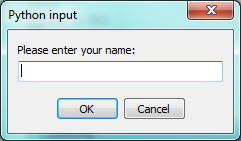
\includegraphics{enter_name_dialog.png}
\end{quote}

The user of the program can enter the name and click \emph{OK}, and when this happens
the text that has been entered is returned from the \code{input} function, and in this
case assigned to the variable \code{n}.

Even if you asked the user to enter their age, you would get back a string like \code{"17"}.
It would be your job, as the programmer, to convert that string into a int or a float,
using the \code{int} or \code{float} converter functions we saw earlier.

\index{composition of functions}\index{function composition}

\section{Composition}
\label{variables_expressions_statements:composition}\label{variables_expressions_statements:index-11}
So far, we have looked at the elements of a program --- variables, expressions,
statements, and function calls --- in isolation, without talking about how to combine them.

One of the most useful features of programming languages is their ability to
take small building blocks and \textbf{compose} them into larger chunks.

For example, we know how to get the user to enter some input, we know how to
convert the string we get into a float, we know how to write a complex expression, and
we know how to print values. Let's put these together in a small four-step program that
asks the user to input a value for the radius of a circle, and then
computes the area of the circle from the formula
\begin{quote}

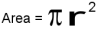
\includegraphics{circle_area.png}
\end{quote}

Firstly, we'll do the four steps one at a time:
\begin{quote}

\begin{Verbatim}[commandchars=\\\{\},numbers=left,firstnumber=1,stepnumber=1]
\PYG{n}{response} \PYG{o}{=} \PYG{n+nb}{input}\PYG{p}{(}\PYG{l+s}{"}\PYG{l+s}{What is your radius? }\PYG{l+s}{"}\PYG{p}{)}
\PYG{n}{r} \PYG{o}{=} \PYG{n+nb}{float}\PYG{p}{(}\PYG{n}{response}\PYG{p}{)}
\PYG{n}{area} \PYG{o}{=} \PYG{l+m+mf}{3.14159} \PYG{o}{*} \PYG{n}{r}\PYG{o}{*}\PYG{o}{*}\PYG{l+m+mi}{2}
\PYG{n+nb}{print}\PYG{p}{(}\PYG{l+s}{"}\PYG{l+s}{The area is }\PYG{l+s}{"}\PYG{p}{,} \PYG{n}{area}\PYG{p}{)}
\end{Verbatim}
\end{quote}

Now let's compose the first two lines into a single line of code, and compose the
second two lines into another line of code.
\begin{quote}

\begin{Verbatim}[commandchars=\\\{\},numbers=left,firstnumber=1,stepnumber=1]
\PYG{n}{r} \PYG{o}{=} \PYG{n+nb}{float}\PYG{p}{(} \PYG{n+nb}{input}\PYG{p}{(}\PYG{l+s}{"}\PYG{l+s}{What is your radius? }\PYG{l+s}{"}\PYG{p}{)} \PYG{p}{)}
\PYG{n+nb}{print}\PYG{p}{(}\PYG{l+s}{"}\PYG{l+s}{The area is }\PYG{l+s}{"}\PYG{p}{,} \PYG{l+m+mf}{3.14159} \PYG{o}{*} \PYG{n}{r}\PYG{o}{*}\PYG{o}{*}\PYG{l+m+mi}{2}\PYG{p}{)}
\end{Verbatim}
\end{quote}

If we really wanted to be tricky, we could write it all in one statement:
\begin{quote}

\begin{Verbatim}[commandchars=\\\{\},numbers=left,firstnumber=1,stepnumber=1]
\PYG{n+nb}{print}\PYG{p}{(}\PYG{l+s}{"}\PYG{l+s}{The area is }\PYG{l+s}{"}\PYG{p}{,} \PYG{l+m+mf}{3.14159}\PYG{o}{*}\PYG{n+nb}{float}\PYG{p}{(}\PYG{n+nb}{input}\PYG{p}{(}\PYG{l+s}{"}\PYG{l+s}{What is your radius?}\PYG{l+s}{"}\PYG{p}{)}\PYG{p}{)}\PYG{o}{*}\PYG{o}{*}\PYG{l+m+mi}{2}\PYG{p}{)}
\end{Verbatim}
\end{quote}

Such compact code may not be most understandable for humans, but it does
illustrate how we can compose bigger chunks from our building blocks.

If you're ever in doubt about whether to compose code or fragment it into smaller steps,
try to make it as simple as you can for the human to follow.  My choice would
be the first case above, with four separate steps.

\index{modulus operator}\index{operator!modulus}

\section{The modulus operator}
\label{variables_expressions_statements:index-12}\label{variables_expressions_statements:the-modulus-operator}
The \textbf{modulus operator} works on integers (and integer expressions) and gives
the remainder when the first number is divided by the second. In Python, the
modulus operator is a percent sign (\code{\%}). The syntax is the same as for other
operators. It has the same precedence as the multiplication operator.
\begin{quote}

\begin{Verbatim}[commandchars=\\\{\}]
\PYG{g+gp}{\PYGZgt{}\PYGZgt{}\PYGZgt{} }\PYG{n}{q} \PYG{o}{=} \PYG{l+m+mi}{7} \PYG{o}{/}\PYG{o}{/} \PYG{l+m+mi}{3}     \PYG{c}{\PYGZsh{} This is integer division operator}
\PYG{g+gp}{\PYGZgt{}\PYGZgt{}\PYGZgt{} }\PYG{n+nb}{print}\PYG{p}{(}\PYG{n}{q}\PYG{p}{)}
\PYG{g+go}{2}
\PYG{g+gp}{\PYGZgt{}\PYGZgt{}\PYGZgt{} }\PYG{n}{r}  \PYG{o}{=} \PYG{l+m+mi}{7} \PYG{o}{\PYGZpc{}} \PYG{l+m+mi}{3}
\PYG{g+gp}{\PYGZgt{}\PYGZgt{}\PYGZgt{} }\PYG{n+nb}{print}\PYG{p}{(}\PYG{n}{r}\PYG{p}{)}
\PYG{g+go}{1}
\end{Verbatim}
\end{quote}

So 7 divided by 3 is 2 with a remainder of 1.

The modulus operator turns out to be surprisingly useful. For example, you can
check whether one number is divisible by another---if \code{x \% y} is zero, then
\code{x} is divisible by \code{y}.

Also, you can extract the right-most digit or digits from a number.  For
example, \code{x \% 10} yields the right-most digit of \code{x} (in base 10).
Similarly \code{x \% 100} yields the last two digits.

It is also extremely useful for doing conversions, say from seconds,
to hours, minutes and seconds. So let's write a program to ask the user to enter
some seconds, and we'll convert them into hours, minutes, and remaining seconds.
\begin{quote}

\begin{Verbatim}[commandchars=\\\{\},numbers=left,firstnumber=1,stepnumber=1]
\PYG{n}{total\PYGZus{}secs} \PYG{o}{=} \PYG{n+nb}{int}\PYG{p}{(}\PYG{n+nb}{input}\PYG{p}{(}\PYG{l+s}{"}\PYG{l+s}{How many seconds, in total?}\PYG{l+s}{"}\PYG{p}{)}\PYG{p}{)}
\PYG{n}{hours} \PYG{o}{=} \PYG{n}{total\PYGZus{}secs} \PYG{o}{/}\PYG{o}{/} \PYG{l+m+mi}{3600}
\PYG{n}{secs\PYGZus{}still\PYGZus{}remaining} \PYG{o}{=} \PYG{n}{total\PYGZus{}secs} \PYG{o}{\PYGZpc{}} \PYG{l+m+mi}{3600}
\PYG{n}{minutes} \PYG{o}{=}  \PYG{n}{secs\PYGZus{}still\PYGZus{}remaining} \PYG{o}{/}\PYG{o}{/} \PYG{l+m+mi}{60}
\PYG{n}{secs\PYGZus{}finally\PYGZus{}remaining} \PYG{o}{=} \PYG{n}{secs\PYGZus{}still\PYGZus{}remaining}  \PYG{o}{\PYGZpc{}} \PYG{l+m+mi}{60}

\PYG{n+nb}{print}\PYG{p}{(}\PYG{l+s}{"}\PYG{l+s}{Hrs=}\PYG{l+s}{"}\PYG{p}{,} \PYG{n}{hours}\PYG{p}{,} \PYG{l+s}{"}\PYG{l+s}{  mins=}\PYG{l+s}{"}\PYG{p}{,} \PYG{n}{minutes}\PYG{p}{,}
                         \PYG{l+s}{"}\PYG{l+s}{secs=}\PYG{l+s}{"}\PYG{p}{,} \PYG{n}{secs\PYGZus{}finally\PYGZus{}remaining}\PYG{p}{)}
\end{Verbatim}
\end{quote}


\section{Glossary}
\label{variables_expressions_statements:glossary}\begin{description}
\item[{\index{assignment statement|textbf}assignment statement}] \leavevmode\phantomsection\label{variables_expressions_statements:term-assignment-statement}
A statement that assigns a value to a name (variable). To the left of
the assignment operator, \code{=}, is a name. To the right of the
assignment token is an expression which is evaluated by the Python
interpreter and then assigned to the name. The difference between the
left and right hand sides of the assignment statement is often
confusing to new programmers. In the following assignment:
\begin{quote}

\begin{Verbatim}[commandchars=\\\{\}]
\PYG{n}{n} \PYG{o}{=} \PYG{n}{n} \PYG{o}{+} \PYG{l+m+mi}{1}
\end{Verbatim}
\end{quote}

\code{n} plays a very different role on each side of the \code{=}. On the
right it is a \emph{value} and makes up part of the \emph{expression} which will
be evaluated by the Python interpreter before assigning it to the name
on the left.

\item[{\index{assignment token|textbf}assignment token}] \leavevmode\phantomsection\label{variables_expressions_statements:term-assignment-token}
\code{=} is Python's assignment token.  Do not confuse it with \emph{equals}, which
is an operator for comparing values.

\item[{\index{composition|textbf}composition}] \leavevmode\phantomsection\label{variables_expressions_statements:term-composition}
The ability to combine simple expressions and statements into compound
statements and expressions in order to represent complex computations
concisely.

\item[{\index{concatenate|textbf}concatenate}] \leavevmode\phantomsection\label{variables_expressions_statements:term-concatenate}
To join two strings end-to-end.

\item[{\index{data type|textbf}data type}] \leavevmode\phantomsection\label{variables_expressions_statements:term-data-type}
A set of values. The type of a value determines how it can be used in
expressions. So far, the types you have seen are integers (\code{int}),
floating-point numbers (\code{float}), and strings (\code{str}).

\item[{\index{evaluate|textbf}evaluate}] \leavevmode\phantomsection\label{variables_expressions_statements:term-evaluate}
To simplify an expression by performing the operations in order to
yield a single value.

\item[{\index{expression|textbf}expression}] \leavevmode\phantomsection\label{variables_expressions_statements:term-expression}
A combination of variables, operators, and values that represents a
single result value.

\item[{\index{float|textbf}float}] \leavevmode\phantomsection\label{variables_expressions_statements:term-float}
A Python data type which stores \emph{floating-point} numbers.
Floating-point numbers are stored internally in two parts: a \emph{base} and
an \emph{exponent}. When printed in the standard format, they look like
decimal numbers. Beware of rounding errors when you use \code{float}s,
and remember that they are only approximate values.

\item[{\index{floor division|textbf}floor division}] \leavevmode\phantomsection\label{variables_expressions_statements:term-floor-division}
An operator (denoted by the token \code{//}) that divides one number by another and
yields an integer, or, if the result is not already an integer, it yields
the next smallest integer.

\item[{\index{int|textbf}int}] \leavevmode\phantomsection\label{variables_expressions_statements:term-int}
A Python data type that holds positive and negative whole numbers.

\item[{\index{keyword|textbf}keyword}] \leavevmode\phantomsection\label{variables_expressions_statements:term-keyword}
A reserved word that is used by the compiler to parse program; you
cannot use keywords like \code{if}, \code{def}, and \code{while} as variable
names.

\item[{\index{modulus operator|textbf}modulus operator}] \leavevmode\phantomsection\label{variables_expressions_statements:term-modulus-operator}
An operator, denoted with a percent sign ( \code{\%}), that works on
integers and yields the remainder when one number is divided by
another.

\item[{\index{operand|textbf}operand}] \leavevmode\phantomsection\label{variables_expressions_statements:term-operand}
One of the values on which an operator operates.

\item[{\index{operator|textbf}operator}] \leavevmode\phantomsection\label{variables_expressions_statements:term-operator}
A special symbol that represents a simple computation like addition,
multiplication, or string concatenation.

\item[{\index{rules of precedence|textbf}rules of precedence}] \leavevmode\phantomsection\label{variables_expressions_statements:term-rules-of-precedence}
The set of rules governing the order in which expressions involving
multiple operators and operands are evaluated.

\item[{\index{state snapshot|textbf}state snapshot}] \leavevmode\phantomsection\label{variables_expressions_statements:term-state-snapshot}
A graphical representation of a set of variables and the values to
which they refer, taken at a particular instant during the program's execution.

\item[{\index{statement|textbf}statement}] \leavevmode\phantomsection\label{variables_expressions_statements:term-statement}
An instruction that the Python interpreter can execute.  So far we have
only seen the assignment statement, but we will soon meet the \code{import}
statement and the \code{for} statement.

\item[{\index{str|textbf}str}] \leavevmode\phantomsection\label{variables_expressions_statements:term-str}
A Python data type that holds a string of characters.

\item[{\index{value|textbf}value}] \leavevmode\phantomsection\label{variables_expressions_statements:term-value}
A number or string (or other things to be named later) that can be
stored in a variable or computed in an expression.

\item[{\index{variable|textbf}variable}] \leavevmode\phantomsection\label{variables_expressions_statements:term-variable}
A name that refers to a value.

\item[{\index{variable name|textbf}variable name}] \leavevmode\phantomsection\label{variables_expressions_statements:term-variable-name}
A name given to a variable. Variable names in Python consist of a
sequence of letters (a..z, A..Z, and \_) and digits (0..9) that begins
with a letter.  In best programming practice, variable names should be
chosen so that they describe their use in the program, making the
program \emph{self documenting}.

\end{description}


\section{Exercises}
\label{variables_expressions_statements:exercises}\begin{enumerate}
\item {} 
Take the sentence: \emph{All work and no play makes Jack a dull boy.}
Store each word in a separate variable, then print out the sentence on
one line using \code{print}.

\item {} 
Add parenthesis to the expression \code{6 * 1 - 2} to change its value
from 4 to -6.

\item {} 
Place a comment before a line of code that previously worked, and
record what happens when you rerun the program.

\item {} 
Start the Python interpreter and enter \code{bruce + 4} at the prompt.
This will give you an error:
\begin{quote}

\begin{Verbatim}[commandchars=\\\{\}]
\PYG{n+ne}{NameError}\PYG{p}{:} \PYG{n}{name} \PYG{l+s}{'}\PYG{l+s}{bruce}\PYG{l+s}{'} \PYG{o+ow}{is} \PYG{o+ow}{not} \PYG{n}{defined}
\end{Verbatim}
\end{quote}

Assign a value to \code{bruce} so that \code{bruce + 4} evaluates to \code{10}.

\item {} 
The formula for computing the final amount if one is earning
compound interest is given on Wikipedia as
\begin{quote}

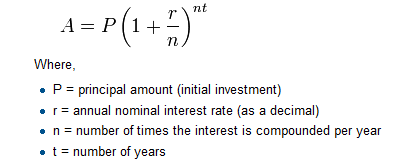
\includegraphics{compoundInterest.png}
\end{quote}

Write a Python program that assigns the principal amount of R10000 to variable \emph{p},
assign to \emph{n} the value 12, and assign to \emph{r} the interest rate of 8\%.
Then have the program prompt the user for the number of years \emph{t} that the money will
be compounded for.  Calculate and print the final amount after \emph{t} years.

\item {} 
Evaluate the following numerical expressions in your head, then use
the Python interpreter to check your results:
\begin{enumerate}
\item {} 
\code{\textgreater{}\textgreater{}\textgreater{} 5 \% 2}

\item {} 
\code{\textgreater{}\textgreater{}\textgreater{} 9 \% 5}

\item {} 
\code{\textgreater{}\textgreater{}\textgreater{} 15 \% 12}

\item {} 
\code{\textgreater{}\textgreater{}\textgreater{} 12 \% 15}

\item {} 
\code{\textgreater{}\textgreater{}\textgreater{} 6 \% 6}

\item {} 
\code{\textgreater{}\textgreater{}\textgreater{} 0 \% 7}

\item {} 
\code{\textgreater{}\textgreater{}\textgreater{} 7 \% 0}

\end{enumerate}

What happened with the last example? Why? If you were able to correctly
anticipate the computer's response in all but the last one, it is time to
move on. If not, take time now to make up examples of your own. Explore the
modulus operator until you are confident you understand how it works.

\item {} 
You look at the clock and it is exactly 2pm.  You set an alarm to go off
in 51 hours.  At what time does the alarm go off?  (Hint: you could count on
your fingers, but this is not what we're after.  If you are tempted
to count on your fingers, change the 51 to 5100.)

\item {} 
Write a Python program to solve the general version of the above problem.
Ask the user for the time now (in hours), and ask for the number of hours to wait.
Your program should output what the time will be on the clock when the alarm goes off.

\end{enumerate}

\begin{DUlineblock}{0em}
\item[] 
\end{DUlineblock}


\chapter{Hello, little turtles!}
\label{hello_little_turtles::doc}\label{hello_little_turtles:hello-little-turtles}
\index{module}\index{function}\index{function definition}\index{definition!function}\index{turtle module}
There are many \emph{modules} in Python that provide very powerful features that we
can use in our own programs.  Some of these can send email, or fetch web pages.
The one we'll look at in this chapter allows us to create turtles and get them
to draw shapes and patterns.

The turtles are fun, but the real purpose of the chapter is to teach ourselves
a little more Python, and to develop our theme of \emph{computational thinking},
or \emph{thinking like a computer scientist}.  Most of the Python covered here
will be explored in more depth later.

\index{object}\index{invoke}\index{method}\index{attribute}\index{state}\index{canvas}

\section{Our first turtle program}
\label{hello_little_turtles:our-first-turtle-program}\label{hello_little_turtles:index-1}
Let's write a couple of lines of Python program to create a new
turtle and start drawing a rectangle. (We'll call the variable that
refers to our first turtle \code{alex}, but we can choose another
name if we follow the naming rules from the previous chapter).
\begin{quote}

\begin{Verbatim}[commandchars=\\\{\},numbers=left,firstnumber=1,stepnumber=1]
 \PYG{k+kn}{import} \PYG{n+nn}{turtle}             \PYG{c}{\PYGZsh{} Allows us to use turtles}
 \PYG{n}{wn} \PYG{o}{=} \PYG{n}{turtle}\PYG{o}{.}\PYG{n}{Screen}\PYG{p}{(}\PYG{p}{)}      \PYG{c}{\PYGZsh{} Creates a playground for turtles}
 \PYG{n}{alex} \PYG{o}{=} \PYG{n}{turtle}\PYG{o}{.}\PYG{n}{Turtle}\PYG{p}{(}\PYG{p}{)}    \PYG{c}{\PYGZsh{} Create a turtle, assign to alex}

 \PYG{n}{alex}\PYG{o}{.}\PYG{n}{forward}\PYG{p}{(}\PYG{l+m+mi}{50}\PYG{p}{)}          \PYG{c}{\PYGZsh{} Tell alex to move forward by 50 units}
 \PYG{n}{alex}\PYG{o}{.}\PYG{n}{left}\PYG{p}{(}\PYG{l+m+mi}{90}\PYG{p}{)}             \PYG{c}{\PYGZsh{} Tell alex to turn by 90 degrees}
 \PYG{n}{alex}\PYG{o}{.}\PYG{n}{forward}\PYG{p}{(}\PYG{l+m+mi}{30}\PYG{p}{)}          \PYG{c}{\PYGZsh{} Complete the second side of a rectangle}

 \PYG{n}{wn}\PYG{o}{.}\PYG{n}{mainloop}\PYG{p}{(}\PYG{p}{)}             \PYG{c}{\PYGZsh{} Wait for user to close window}
\end{Verbatim}
\end{quote}

When we run this program, a new window pops up:
\begin{quote}

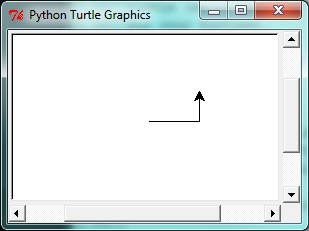
\includegraphics{tess01.png}
\end{quote}

Here are a couple of things we'll need to understand about this program.

The first line tells Python to load a module named \code{turtle}.
That module brings us two new types that we can use:
the \code{Turtle} type, and the \code{Screen} type.  The dot
notation \code{turtle.Turtle} means \emph{``The Turtle type that is defined within
the turtle module''}.   (Remember that Python is case sensitive, so the
module name, with a lowercase \emph{t}, is different from the type \code{Turtle}.)

We then create and open what it calls a screen (we would prefer to call it
a window), which we assign to variable \code{wn}. Every window contains
a \textbf{canvas}, which is the area inside the window on which we can draw.

In line 3 we create a turtle. The variable \code{alex} is made to refer to this turtle.

So these first three lines have set things up, we're ready to get our turtle to draw on our canvas.

In lines 5-7, we instruct the \textbf{object} \code{alex} to move, and to turn. We
do this by \textbf{invoking}, or activating, \code{alex}`s \textbf{methods} --- these are
the instructions that all turtles know how to respond to.

The last line plays a part too: the \code{wn} variable refers to
the window shown above. When we invoke its \code{mainloop} method, it enters
a state where it waits for events (like keypresses, or mouse movement and clicks).
The program will terminate when the user closes the window.

An object can have various methods --- things it can do --- and it can also have
\textbf{attributes} --- (sometimes called \emph{properties}).  For example, each turtle has
a \emph{color} attribute.  The method invocation
\code{alex.color("red")} will make \code{alex} red, and drawing will be red too.
(Note the word \emph{color}  is spelled the American way!)

The color of the turtle, the width of its pen, the position of the
turtle within the window, which way it is facing, and so on are all part of its
current \textbf{state}.   Similarly, the window object has a background color, and
some text in the title bar, and a size and position on the screen.  These are all
part of the state of the window object.

Quite a number of methods exist that allow us to modify the turtle and the
window objects.  We'll just show a couple. In this program we've only commented those
lines that are different from the previous example (and we've used a different
variable name for this turtle):
\begin{quote}

\begin{Verbatim}[commandchars=\\\{\},numbers=left,firstnumber=1,stepnumber=1]
 \PYG{k+kn}{import} \PYG{n+nn}{turtle}
 \PYG{n}{wn} \PYG{o}{=} \PYG{n}{turtle}\PYG{o}{.}\PYG{n}{Screen}\PYG{p}{(}\PYG{p}{)}
 \PYG{n}{wn}\PYG{o}{.}\PYG{n}{bgcolor}\PYG{p}{(}\PYG{l+s}{"}\PYG{l+s}{lightgreen}\PYG{l+s}{"}\PYG{p}{)}      \PYG{c}{\PYGZsh{} Set the window background color}
 \PYG{n}{wn}\PYG{o}{.}\PYG{n}{title}\PYG{p}{(}\PYG{l+s}{"}\PYG{l+s}{Hello, Tess!}\PYG{l+s}{"}\PYG{p}{)}      \PYG{c}{\PYGZsh{} Set the window title}

 \PYG{n}{tess} \PYG{o}{=} \PYG{n}{turtle}\PYG{o}{.}\PYG{n}{Turtle}\PYG{p}{(}\PYG{p}{)}
 \PYG{n}{tess}\PYG{o}{.}\PYG{n}{color}\PYG{p}{(}\PYG{l+s}{"}\PYG{l+s}{blue}\PYG{l+s}{"}\PYG{p}{)}            \PYG{c}{\PYGZsh{} Tell tess to change her color}
 \PYG{n}{tess}\PYG{o}{.}\PYG{n}{pensize}\PYG{p}{(}\PYG{l+m+mi}{3}\PYG{p}{)}               \PYG{c}{\PYGZsh{} Tell tess to set her pen width}

 \PYG{n}{tess}\PYG{o}{.}\PYG{n}{forward}\PYG{p}{(}\PYG{l+m+mi}{50}\PYG{p}{)}
 \PYG{n}{tess}\PYG{o}{.}\PYG{n}{left}\PYG{p}{(}\PYG{l+m+mi}{120}\PYG{p}{)}
 \PYG{n}{tess}\PYG{o}{.}\PYG{n}{forward}\PYG{p}{(}\PYG{l+m+mi}{50}\PYG{p}{)}

 \PYG{n}{wn}\PYG{o}{.}\PYG{n}{mainloop}\PYG{p}{(}\PYG{p}{)}
\end{Verbatim}
\end{quote}

When we run this program, this new window pops up, and will remain on the
screen until we close it.
\begin{quote}

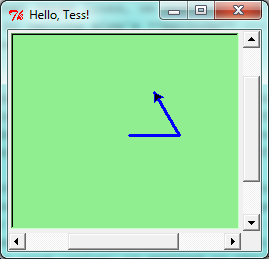
\includegraphics{tess02.png}
\end{quote}

\begin{notice}{note}{Extend this program ...}
\begin{enumerate}
\item {} 
Modify this program so that before it creates the window, it prompts
the user to enter the desired background color. It should store the user's
responses in a variable, and modify the color of the window
according to the user's wishes.
(Hint: you can find a list of permitted color names at
\href{http://www.tcl.tk/man/tcl8.4/TkCmd/colors.htm}{http://www.tcl.tk/man/tcl8.4/TkCmd/colors.htm}.  It includes some quite unusual
ones, like ``peach puff''  and ``HotPink''.)

\item {} 
Do similar changes to allow the user, at runtime, to set \code{tess}` color.

\item {} 
Do the same for the width of \code{tess}` pen.  \emph{Hint:} your dialog with the
user will return a string, but \code{tess}` \code{pensize} method
expects its argument to be an int.  So you'll need to convert
the string to an int before you pass it to \code{pensize}.

\end{enumerate}
\end{notice}

\index{instance}

\section{Instances --- a herd of turtles}
\label{hello_little_turtles:index-2}\label{hello_little_turtles:instances-a-herd-of-turtles}
Just like we can have many different integers in a program, we can have many turtles.
Each of them is called an \textbf{instance}.  Each instance has its own attributes and
methods --- so \code{alex} might draw with a thin black pen and be at some position,
while \code{tess} might be going in her own direction with a fat pink pen.
\begin{quote}

\begin{Verbatim}[commandchars=\\\{\},numbers=left,firstnumber=1,stepnumber=1]
 \PYG{k+kn}{import} \PYG{n+nn}{turtle}
 \PYG{n}{wn} \PYG{o}{=} \PYG{n}{turtle}\PYG{o}{.}\PYG{n}{Screen}\PYG{p}{(}\PYG{p}{)}         \PYG{c}{\PYGZsh{} Set up the window and its attributes}
 \PYG{n}{wn}\PYG{o}{.}\PYG{n}{bgcolor}\PYG{p}{(}\PYG{l+s}{"}\PYG{l+s}{lightgreen}\PYG{l+s}{"}\PYG{p}{)}
 \PYG{n}{wn}\PYG{o}{.}\PYG{n}{title}\PYG{p}{(}\PYG{l+s}{"}\PYG{l+s}{Tess \PYGZam{} Alex}\PYG{l+s}{"}\PYG{p}{)}

 \PYG{n}{tess} \PYG{o}{=} \PYG{n}{turtle}\PYG{o}{.}\PYG{n}{Turtle}\PYG{p}{(}\PYG{p}{)}       \PYG{c}{\PYGZsh{} Create tess and set some attributes}
 \PYG{n}{tess}\PYG{o}{.}\PYG{n}{color}\PYG{p}{(}\PYG{l+s}{"}\PYG{l+s}{hotpink}\PYG{l+s}{"}\PYG{p}{)}
 \PYG{n}{tess}\PYG{o}{.}\PYG{n}{pensize}\PYG{p}{(}\PYG{l+m+mi}{5}\PYG{p}{)}

 \PYG{n}{alex} \PYG{o}{=} \PYG{n}{turtle}\PYG{o}{.}\PYG{n}{Turtle}\PYG{p}{(}\PYG{p}{)}       \PYG{c}{\PYGZsh{} Create alex}

 \PYG{n}{tess}\PYG{o}{.}\PYG{n}{forward}\PYG{p}{(}\PYG{l+m+mi}{80}\PYG{p}{)}             \PYG{c}{\PYGZsh{} Make tess draw equilateral triangle}
 \PYG{n}{tess}\PYG{o}{.}\PYG{n}{left}\PYG{p}{(}\PYG{l+m+mi}{120}\PYG{p}{)}
 \PYG{n}{tess}\PYG{o}{.}\PYG{n}{forward}\PYG{p}{(}\PYG{l+m+mi}{80}\PYG{p}{)}
 \PYG{n}{tess}\PYG{o}{.}\PYG{n}{left}\PYG{p}{(}\PYG{l+m+mi}{120}\PYG{p}{)}
 \PYG{n}{tess}\PYG{o}{.}\PYG{n}{forward}\PYG{p}{(}\PYG{l+m+mi}{80}\PYG{p}{)}
 \PYG{n}{tess}\PYG{o}{.}\PYG{n}{left}\PYG{p}{(}\PYG{l+m+mi}{120}\PYG{p}{)}               \PYG{c}{\PYGZsh{} Complete the triangle}

 \PYG{n}{tess}\PYG{o}{.}\PYG{n}{right}\PYG{p}{(}\PYG{l+m+mi}{180}\PYG{p}{)}              \PYG{c}{\PYGZsh{} Turn tess around}
 \PYG{n}{tess}\PYG{o}{.}\PYG{n}{forward}\PYG{p}{(}\PYG{l+m+mi}{80}\PYG{p}{)}             \PYG{c}{\PYGZsh{} Move her away from the origin}

 \PYG{n}{alex}\PYG{o}{.}\PYG{n}{forward}\PYG{p}{(}\PYG{l+m+mi}{50}\PYG{p}{)}             \PYG{c}{\PYGZsh{} Make alex draw a square}
 \PYG{n}{alex}\PYG{o}{.}\PYG{n}{left}\PYG{p}{(}\PYG{l+m+mi}{90}\PYG{p}{)}
 \PYG{n}{alex}\PYG{o}{.}\PYG{n}{forward}\PYG{p}{(}\PYG{l+m+mi}{50}\PYG{p}{)}
 \PYG{n}{alex}\PYG{o}{.}\PYG{n}{left}\PYG{p}{(}\PYG{l+m+mi}{90}\PYG{p}{)}
 \PYG{n}{alex}\PYG{o}{.}\PYG{n}{forward}\PYG{p}{(}\PYG{l+m+mi}{50}\PYG{p}{)}
 \PYG{n}{alex}\PYG{o}{.}\PYG{n}{left}\PYG{p}{(}\PYG{l+m+mi}{90}\PYG{p}{)}
 \PYG{n}{alex}\PYG{o}{.}\PYG{n}{forward}\PYG{p}{(}\PYG{l+m+mi}{50}\PYG{p}{)}
 \PYG{n}{alex}\PYG{o}{.}\PYG{n}{left}\PYG{p}{(}\PYG{l+m+mi}{90}\PYG{p}{)}

 \PYG{n}{wn}\PYG{o}{.}\PYG{n}{mainloop}\PYG{p}{(}\PYG{p}{)}
\end{Verbatim}
\end{quote}

Here is what happens when \code{alex} completes his rectangle, and \code{tess} completes her triangle:
\begin{quote}

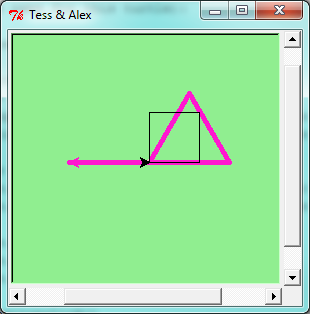
\includegraphics{tess03.png}
\end{quote}

Here are some \emph{How to think like a computer scientist} observations:
\begin{itemize}
\item {} 
There are 360 degrees in a full circle.  If we add up all the turns that a turtle makes,
\emph{no matter what steps occurred between the turns}, we can easily figure out if they
add up to some multiple of 360.  This should convince us that \code{alex} is facing in
exactly the same direction as he was when he was first created. (Geometry
conventions have 0 degrees facing East, and that is the case here too!)

\item {} 
We could have left out the last turn for \code{alex}, but that would not have been
as satisfying.  If we're asked to draw a closed shape like a
square or a rectangle, it is a good idea to
complete all the turns and to leave the turtle back where it started, facing the
same direction as it started in.
This makes reasoning about the program and composing chunks of code into bigger programs
easier for us humans!

\item {} 
We did the same with \code{tess}: she drew her triangle, and turned through a full 360 degrees.
Then we turned her around and moved her aside.  Even the blank line 18
is a hint about how the programmer's \emph{mental chunking} is working:
in big terms, \code{tess}` movements were chunked as ``draw the triangle''
(lines 12-17) and then ``move away from the origin'' (lines 19 and 20).

\item {} 
One of the key uses for comments is to record our mental chunking, and big ideas.
They're not always explicit in the code.

\item {} 
And, uh-huh, two turtles may not be enough for a herd. But the important idea is that the
turtle module gives us a kind of factory that lets us create as many turtles as we
need. Each instance has its own state and behaviour.

\end{itemize}

\index{for loop}

\section{The \textbf{for} loop}
\label{hello_little_turtles:the-for-loop}\label{hello_little_turtles:index-3}
When we drew the square, it was quite tedious.  We had to explicitly repeat the steps of
moving and turning four times.  If we were drawing a hexagon, or an octogon,
or a polygon with 42 sides, it would have been worse.

So a basic building block of all programs is to be able to repeat some code, over and
over again.

Python's \textbf{for} loop solves this for us.   Let's say we have some friends, and
we'd like to send them each an email inviting them to our party.  We don't
quite know how to send email yet, so for the moment we'll just print a message for each friend:
\begin{quote}

\begin{Verbatim}[commandchars=\\\{\},numbers=left,firstnumber=1,stepnumber=1]
\PYG{k}{for} \PYG{n}{f} \PYG{o+ow}{in} \PYG{p}{[}\PYG{l+s}{"}\PYG{l+s}{Joe}\PYG{l+s}{"}\PYG{p}{,}\PYG{l+s}{"}\PYG{l+s}{Zoe}\PYG{l+s}{"}\PYG{p}{,}\PYG{l+s}{"}\PYG{l+s}{Brad}\PYG{l+s}{"}\PYG{p}{,}\PYG{l+s}{"}\PYG{l+s}{Angelina}\PYG{l+s}{"}\PYG{p}{,}\PYG{l+s}{"}\PYG{l+s}{Zuki}\PYG{l+s}{"}\PYG{p}{,}\PYG{l+s}{"}\PYG{l+s}{Thandi}\PYG{l+s}{"}\PYG{p}{,}\PYG{l+s}{"}\PYG{l+s}{Paris}\PYG{l+s}{"}\PYG{p}{]}\PYG{p}{:}
    \PYG{n}{invite} \PYG{o}{=} \PYG{l+s}{"}\PYG{l+s}{Hi }\PYG{l+s}{"} \PYG{o}{+} \PYG{n}{f} \PYG{o}{+} \PYG{l+s}{"}\PYG{l+s}{.  Please come to my party on Saturday!}\PYG{l+s}{"}
    \PYG{n+nb}{print}\PYG{p}{(}\PYG{n}{invite}\PYG{p}{)}
\PYG{c}{\PYGZsh{} more code can follow here ...}
\end{Verbatim}
\end{quote}

When we run this, the output looks like this:
\begin{quote}

\begin{Verbatim}[commandchars=\\\{\}]
\PYG{g+go}{Hi Joe.  Please come to my party on Saturday!}
\PYG{g+go}{Hi Zoe.  Please come to my party on Saturday!}
\PYG{g+go}{Hi Brad.  Please come to my party on Saturday!}
\PYG{g+go}{Hi Angelina.  Please come to my party on Saturday!}
\PYG{g+go}{Hi Zuki.  Please come to my party on Saturday!}
\PYG{g+go}{Hi Thandi.  Please come to my party on Saturday!}
\PYG{g+go}{Hi Paris.  Please come to my party on Saturday!}
\end{Verbatim}
\end{quote}
\begin{itemize}
\item {} 
The variable \code{f} in the \code{for} statement at line 1 is called the \textbf{loop variable}.
We could have chosen any other variable name instead.

\item {} 
Lines 2 and 3 are the \textbf{loop body}.  The loop body is always
indented. The indentation determines exactly what statements are ``in the body of the loop''.

\item {} 
On each \emph{iteration} or \emph{pass} of the loop, first a check is done to see if there are
still more items to be processed.  If there are none left (this is called
the \textbf{terminating condition} of the loop), the loop has finished.
Program execution continues at the next statement after the loop body, (e.g. in this case
the next statement below the comment in line 4).

\item {} 
If there are items still to be processed, the loop variable is updated to refer to the
next item in the list.  This means, in this case, that the loop body is executed
here 7 times, and each time \code{f} will refer to a different friend.

\item {} 
At the end of each execution of the body of the loop, Python returns
to the \code{for} statement, to see if there are more items to be handled, and to assign the
next one to \code{f}.

\end{itemize}

\index{control flow}\index{flow of execution}

\section{Flow of Execution of the for loop}
\label{hello_little_turtles:index-4}\label{hello_little_turtles:flow-of-execution-of-the-for-loop}
As a program executes, the interpreter always keeps track of which statement is
about to be executed.  We call this the \textbf{control flow}, of the \textbf{flow of execution}
of the program.  When humans execute programs, they often use their finger to point
to each statement in turn.  So we could think of control flow as ``Python's moving finger''.

Control flow until now has been strictly
top to bottom, one statement at a time.  The \code{for} loop changes this.

\begin{notice}{note}{Flowchart of a \textbf{for} loop}

Control flow is often easy to visualize and understand if we draw a flowchart.
This shows the exact steps and logic of how the \code{for} statement executes.

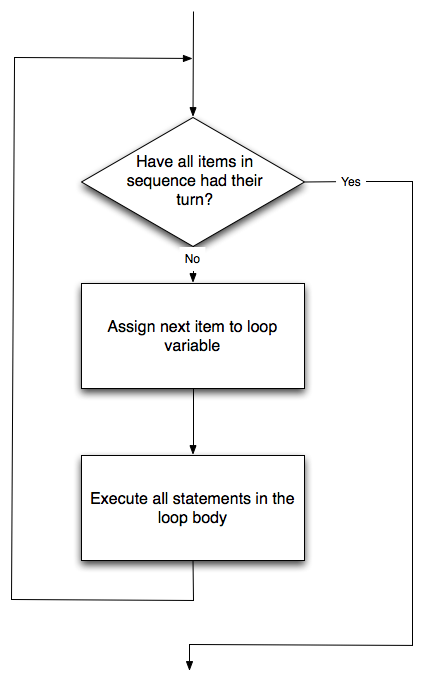
\includegraphics{flowchart_for.png}
\end{notice}

\index{range function}\index{chunking}

\section{The loop simplifies our turtle program}
\label{hello_little_turtles:index-5}\label{hello_little_turtles:the-loop-simplifies-our-turtle-program}
To draw a square we'd like to do the same thing four times --- move the turtle, and turn.
We previously used 8 lines to have \code{alex} draw the four sides of a square.
This does exactly the same, but using just three lines:
\begin{quote}

\begin{Verbatim}[commandchars=\\\{\},numbers=left,firstnumber=1,stepnumber=1]
\PYG{k}{for} \PYG{n}{i} \PYG{o+ow}{in} \PYG{p}{[}\PYG{l+m+mi}{0}\PYG{p}{,}\PYG{l+m+mi}{1}\PYG{p}{,}\PYG{l+m+mi}{2}\PYG{p}{,}\PYG{l+m+mi}{3}\PYG{p}{]}\PYG{p}{:}
    \PYG{n}{alex}\PYG{o}{.}\PYG{n}{forward}\PYG{p}{(}\PYG{l+m+mi}{50}\PYG{p}{)}
    \PYG{n}{alex}\PYG{o}{.}\PYG{n}{left}\PYG{p}{(}\PYG{l+m+mi}{90}\PYG{p}{)}
\end{Verbatim}
\end{quote}

Some observations:
\begin{itemize}
\item {} 
While ``saving some lines of code'' might be convenient, it is not the big deal here.
What is much more important is that we've found a ``repeating pattern'' of statements,
and reorganized our program to repeat the pattern.  Finding the chunks and somehow
getting our programs arranged around those chunks is a vital
skill in computational thinking.

\item {} 
The values {[}0,1,2,3{]} were provided to make the loop body execute 4 times.
We could
have used any four values, but these are the conventional ones to use.  In fact, they are
so popular that Python gives us special built-in \code{range} objects:
\begin{quote}

\begin{Verbatim}[commandchars=\\\{\},numbers=left,firstnumber=1,stepnumber=1]
\PYG{k}{for} \PYG{n}{i} \PYG{o+ow}{in} \PYG{n+nb}{range}\PYG{p}{(}\PYG{l+m+mi}{4}\PYG{p}{)}\PYG{p}{:}
    \PYG{c}{\PYGZsh{} Executes the body with i = 0, then 1, then 2, then 3}
\PYG{k}{for} \PYG{n}{x} \PYG{o+ow}{in} \PYG{n+nb}{range}\PYG{p}{(}\PYG{l+m+mi}{10}\PYG{p}{)}\PYG{p}{:}
    \PYG{c}{\PYGZsh{} Sets x to each of ... [0, 1, 2, 3, 4, 5, 6, 7, 8, 9]}
\end{Verbatim}
\end{quote}

\item {} 
Computer scientists like to count from 0!

\item {} 
\code{range} can deliver a sequence of values to the loop variable in the \code{for} loop.
They start at 0, and in these cases do not include the 4 or the 10.

\item {} 
Our little trick earlier to make sure that \code{alex} did the final turn to complete
360 degrees has paid off: if we had not done that, then we would not have been
able to use a loop for the fourth side of the square.
It would have become a ``special case'',
different from the other sides.  When possible, we'd much prefer to make
our code fit a general pattern, rather than have to create a special case.

\end{itemize}

So to repeat something four times, a good Python programmer would do this:
\begin{quote}

\begin{Verbatim}[commandchars=\\\{\},numbers=left,firstnumber=1,stepnumber=1]
\PYG{k}{for} \PYG{n}{i} \PYG{o+ow}{in} \PYG{n+nb}{range}\PYG{p}{(}\PYG{l+m+mi}{4}\PYG{p}{)}\PYG{p}{:}
    \PYG{n}{alex}\PYG{o}{.}\PYG{n}{forward}\PYG{p}{(}\PYG{l+m+mi}{50}\PYG{p}{)}
    \PYG{n}{alex}\PYG{o}{.}\PYG{n}{left}\PYG{p}{(}\PYG{l+m+mi}{90}\PYG{p}{)}
\end{Verbatim}
\end{quote}

By now you should be able to see how to change our previous program so that
\code{tess} can also use a \code{for} loop to draw her equilateral triangle.

But now, what would happen if we made this change?
\begin{quote}

\begin{Verbatim}[commandchars=\\\{\},numbers=left,firstnumber=1,stepnumber=1]
\PYG{k}{for} \PYG{n}{c} \PYG{o+ow}{in} \PYG{p}{[}\PYG{l+s}{"}\PYG{l+s}{yellow}\PYG{l+s}{"}\PYG{p}{,} \PYG{l+s}{"}\PYG{l+s}{red}\PYG{l+s}{"}\PYG{p}{,} \PYG{l+s}{"}\PYG{l+s}{purple}\PYG{l+s}{"}\PYG{p}{,} \PYG{l+s}{"}\PYG{l+s}{blue}\PYG{l+s}{"}\PYG{p}{]}\PYG{p}{:}
    \PYG{n}{alex}\PYG{o}{.}\PYG{n}{color}\PYG{p}{(}\PYG{n}{c}\PYG{p}{)}
    \PYG{n}{alex}\PYG{o}{.}\PYG{n}{forward}\PYG{p}{(}\PYG{l+m+mi}{50}\PYG{p}{)}
    \PYG{n}{alex}\PYG{o}{.}\PYG{n}{left}\PYG{p}{(}\PYG{l+m+mi}{90}\PYG{p}{)}
\end{Verbatim}
\end{quote}

A variable can also be assigned a value that is a list.  So lists can also be used in
more general situations, not only in the \code{for} loop.  The code above could be rewritten like this:
\begin{quote}

\begin{Verbatim}[commandchars=\\\{\},numbers=left,firstnumber=1,stepnumber=1]
\PYG{c}{\PYGZsh{} Assign a list to a variable}
\PYG{n}{clrs} \PYG{o}{=} \PYG{p}{[}\PYG{l+s}{"}\PYG{l+s}{yellow}\PYG{l+s}{"}\PYG{p}{,} \PYG{l+s}{"}\PYG{l+s}{red}\PYG{l+s}{"}\PYG{p}{,} \PYG{l+s}{"}\PYG{l+s}{purple}\PYG{l+s}{"}\PYG{p}{,} \PYG{l+s}{"}\PYG{l+s}{blue}\PYG{l+s}{"}\PYG{p}{]}
\PYG{k}{for} \PYG{n}{c} \PYG{o+ow}{in} \PYG{n}{clrs}\PYG{p}{:}
    \PYG{n}{alex}\PYG{o}{.}\PYG{n}{color}\PYG{p}{(}\PYG{n}{c}\PYG{p}{)}
    \PYG{n}{alex}\PYG{o}{.}\PYG{n}{forward}\PYG{p}{(}\PYG{l+m+mi}{50}\PYG{p}{)}
    \PYG{n}{alex}\PYG{o}{.}\PYG{n}{left}\PYG{p}{(}\PYG{l+m+mi}{90}\PYG{p}{)}
\end{Verbatim}
\end{quote}


\section{A few more turtle methods and tricks}
\label{hello_little_turtles:a-few-more-turtle-methods-and-tricks}
Turtle methods can use negative angles or distances.  So \code{tess.forward(-100)}
will move \code{tess} backwards, and \code{tess.left(-30)} turns her to the right.  Additionally,
because there are 360 degrees in a circle, turning 30 to the left will get \code{tess} facing
in the same direction as turning 330 to the right!  (The on-screen animation will differ,
though --- you will be able to tell if \code{tess} is turning clockwise or counter-clockwise!)

This suggests that we don't need both a left and a right turn method --- we could be
minimalists, and just have one method.  There is also a \emph{backward}
method.  (If you are very nerdy, you might enjoy saying \code{alex.backward(-100)} to
move \code{alex} forward!)

Part of \emph{thinking like a scientist} is to understand more of the structure and rich
relationships in our field.  So revising a few basic facts about
geometry and number lines, and spotting the relationships between left, right,
backward, forward, negative and positive distances or angles values is a good start
if we're going to play with turtles.

A turtle's pen can be picked up or put down.  This allows us to move a turtle
to a different place without drawing a line.   The methods are
\begin{quote}

\begin{Verbatim}[commandchars=\\\{\},numbers=left,firstnumber=1,stepnumber=1]
\PYG{n}{alex}\PYG{o}{.}\PYG{n}{penup}\PYG{p}{(}\PYG{p}{)}
\PYG{n}{alex}\PYG{o}{.}\PYG{n}{forward}\PYG{p}{(}\PYG{l+m+mi}{100}\PYG{p}{)}     \PYG{c}{\PYGZsh{} This moves alex, but no line is drawn}
\PYG{n}{alex}\PYG{o}{.}\PYG{n}{pendown}\PYG{p}{(}\PYG{p}{)}
\end{Verbatim}
\end{quote}

Every turtle can have its own shape.  The ones available ``out of the box''
are \code{arrow}, \code{blank}, \code{circle}, \code{classic}, \code{square}, \code{triangle}, \code{turtle}.
\begin{quote}

\begin{Verbatim}[commandchars=\\\{\},numbers=left,firstnumber=1,stepnumber=1]
\PYG{n}{alex}\PYG{o}{.}\PYG{n}{shape}\PYG{p}{(}\PYG{l+s}{"}\PYG{l+s}{turtle}\PYG{l+s}{"}\PYG{p}{)}
\end{Verbatim}

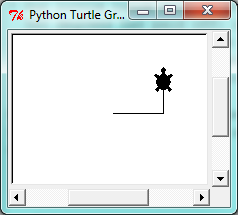
\includegraphics{alex06.png}
\end{quote}

We can speed up or slow down the turtle's animation speed. (Animation controls how
quickly the turtle turns and moves forward).  Speed settings can be set
between 1 (slowest) to 10 (fastest).  But if we set the speed to 0, it has
a special meaning --- turn off animation and go as fast as possible.
\begin{quote}

\begin{Verbatim}[commandchars=\\\{\},numbers=left,firstnumber=1,stepnumber=1]
\PYG{n}{alex}\PYG{o}{.}\PYG{n}{speed}\PYG{p}{(}\PYG{l+m+mi}{10}\PYG{p}{)}
\end{Verbatim}
\end{quote}

A turtle can ``stamp'' its footprint onto the canvas,
and this will remain after the turtle has moved somewhere else.
Stamping works, even when the pen is up.

Let's do an example that shows off some of these new features:
\begin{quote}

\begin{Verbatim}[commandchars=\\\{\},numbers=left,firstnumber=1,stepnumber=1]
\PYG{k+kn}{import} \PYG{n+nn}{turtle}
\PYG{n}{wn} \PYG{o}{=} \PYG{n}{turtle}\PYG{o}{.}\PYG{n}{Screen}\PYG{p}{(}\PYG{p}{)}
\PYG{n}{wn}\PYG{o}{.}\PYG{n}{bgcolor}\PYG{p}{(}\PYG{l+s}{"}\PYG{l+s}{lightgreen}\PYG{l+s}{"}\PYG{p}{)}
\PYG{n}{tess} \PYG{o}{=} \PYG{n}{turtle}\PYG{o}{.}\PYG{n}{Turtle}\PYG{p}{(}\PYG{p}{)}
\PYG{n}{tess}\PYG{o}{.}\PYG{n}{shape}\PYG{p}{(}\PYG{l+s}{"}\PYG{l+s}{turtle}\PYG{l+s}{"}\PYG{p}{)}
\PYG{n}{tess}\PYG{o}{.}\PYG{n}{color}\PYG{p}{(}\PYG{l+s}{"}\PYG{l+s}{blue}\PYG{l+s}{"}\PYG{p}{)}

\PYG{n}{tess}\PYG{o}{.}\PYG{n}{penup}\PYG{p}{(}\PYG{p}{)}                \PYG{c}{\PYGZsh{} This is new}
\PYG{n}{size} \PYG{o}{=} \PYG{l+m+mi}{20}
\PYG{k}{for} \PYG{n}{i} \PYG{o+ow}{in} \PYG{n+nb}{range}\PYG{p}{(}\PYG{l+m+mi}{30}\PYG{p}{)}\PYG{p}{:}
   \PYG{n}{tess}\PYG{o}{.}\PYG{n}{stamp}\PYG{p}{(}\PYG{p}{)}             \PYG{c}{\PYGZsh{} Leave an impression on the canvas}
   \PYG{n}{size} \PYG{o}{=} \PYG{n}{size} \PYG{o}{+} \PYG{l+m+mi}{3}          \PYG{c}{\PYGZsh{} Increase the size on every iteration}
   \PYG{n}{tess}\PYG{o}{.}\PYG{n}{forward}\PYG{p}{(}\PYG{n}{size}\PYG{p}{)}       \PYG{c}{\PYGZsh{} Move tess along}
   \PYG{n}{tess}\PYG{o}{.}\PYG{n}{right}\PYG{p}{(}\PYG{l+m+mi}{24}\PYG{p}{)}           \PYG{c}{\PYGZsh{}  ...  and turn her}

\PYG{n}{wn}\PYG{o}{.}\PYG{n}{mainloop}\PYG{p}{(}\PYG{p}{)}
\end{Verbatim}

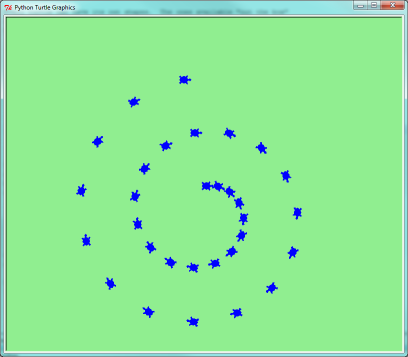
\includegraphics{tess07.png}
\end{quote}

Be careful now!   How many times was the body of the loop executed?   How many turtle
images do we see on the screen?  All except one of the shapes we see on the screen here
are footprints created by \code{stamp}.  But the program still only has \emph{one} turtle
instance --- can you figure out which one here is the real \code{tess}?  (Hint: if you're not
sure, write a new line of code after the \code{for} loop to change \code{tess}` color,
or to put her pen down and draw a line, or to change her shape, etc.)


\section{Glossary}
\label{hello_little_turtles:glossary}\begin{description}
\item[{\index{attribute|textbf}attribute}] \leavevmode\phantomsection\label{hello_little_turtles:term-attribute}
Some state or value that belongs to a particular object.  For example, \code{tess} has
a color.

\item[{\index{canvas|textbf}canvas}] \leavevmode\phantomsection\label{hello_little_turtles:term-canvas}
A surface within a window where drawing takes place.

\item[{\index{control flow|textbf}control flow}] \leavevmode\phantomsection\label{hello_little_turtles:term-control-flow}
See \emph{flow of execution} in the next chapter.

\item[{\index{for loop|textbf}for loop}] \leavevmode\phantomsection\label{hello_little_turtles:term-for-loop}
A statement in Python for convenient repetition of statements in the \emph{body} of the loop.

\item[{\index{loop body|textbf}loop body}] \leavevmode\phantomsection\label{hello_little_turtles:term-loop-body}
Any number of statements nested inside a loop. The nesting is indicated
by the fact that the statements are indented under the for loop statement.

\item[{\index{loop variable|textbf}loop variable}] \leavevmode\phantomsection\label{hello_little_turtles:term-loop-variable}
A variable used as part of a for loop. It is assigned a different value on
each iteration of the loop.

\item[{\index{instance|textbf}instance}] \leavevmode\phantomsection\label{hello_little_turtles:term-instance}
An object of a certain type, or class.  \code{tess} and \code{alex} are different instances of
the class \code{Turtle}.

\item[{\index{method|textbf}method}] \leavevmode\phantomsection\label{hello_little_turtles:term-method}
A function that is attached to an object.  Invoking or activating the method
causes the object to respond in some way, e.g. \code{forward} is the method
when we say \code{tess.forward(100)}.

\item[{\index{invoke|textbf}invoke}] \leavevmode\phantomsection\label{hello_little_turtles:term-invoke}
An object has methods.  We use the verb invoke to mean \emph{activate the
method}.  Invoking a method is done by putting parentheses after the method
name, with some possible arguments.  So  \code{tess.forward()} is an invocation
of the \code{forward} method.

\item[{\index{module|textbf}module}] \leavevmode\phantomsection\label{hello_little_turtles:term-module}
A file containing Python definitions and statements intended for use in other
Python programs. The contents of a module are made available to the other
program by using the \code{import} statement.

\item[{\index{object|textbf}object}] \leavevmode\phantomsection\label{hello_little_turtles:term-object}
A ``thing'' to which a variable can refer.  This could be a screen window,
or one of the turtles we have created.

\item[{\index{range|textbf}range}] \leavevmode\phantomsection\label{hello_little_turtles:term-range}
A built-in function in Python for generating sequences of integers.  It is especially
useful when we need to write a for loop that executes a fixed number of times.

\item[{\index{terminating condition|textbf}terminating condition}] \leavevmode\phantomsection\label{hello_little_turtles:term-terminating-condition}
A condition that occurs which causes a loop to stop repeating its body.
In the \code{for} loops we saw in this chapter, the terminating condition
has been when there are no more elements to assign to the loop variable.

\end{description}


\section{Exercises}
\label{hello_little_turtles:exercises}\begin{enumerate}
\item {} 
Write a program that prints \code{We like Python's turtles!} 1000 times.

\item {} 
Give three attributes of your cellphone object.  Give three methods of your cellphone.

\item {} \begin{description}
\item[{Write a program that uses a for loop to print}] \leavevmode
\begin{DUlineblock}{0em}
\item[] \code{One of the months of the year is January}
\item[] \code{One of the months of the year is February}
\item[] ...
\end{DUlineblock}

\end{description}

\item {} 
Suppose our turtle \code{tess} is at heading 0 --- facing east.  We execute the statement
\code{tess.left(3645)}.  What does \code{tess} do, and what is her final heading?

\item {} 
Assume you have the assignment \code{xs = {[}12, 10, 32, 3, 66, 17, 42, 99, 20{]}}
\begin{enumerate}
\item {} 
Write a loop that prints each of the numbers on a new line.

\item {} 
Write a loop that prints each number and its square on a new line.

\item {} 
Write a loop that adds all the numbers from the list into a variable called \emph{total}.
You should set the \emph{total} variable to have the value 0 before you start adding them up,
and print the value in \code{total} after the loop has completed.

\item {} 
Print the product of all the numbers in the list.
(product means all multiplied together)

\end{enumerate}

\item {} 
Use \code{for} loops to make a turtle draw these regular polygons
(regular means all sides the same lengths, all angles the same):
\begin{itemize}
\item {} 
An equilateral triangle

\item {} 
A square

\item {} 
A hexagon (six sides)

\item {} 
An octagon (eight sides)

\end{itemize}

\item {} \phantomsection\label{hello_little_turtles:drunk-pirate-problem}
A drunk pirate makes a random turn and then takes 100 steps forward, makes another random turn,
takes another 100 steps, turns another random amount, etc.  A social science student records the angle of each turn
before the next 100 steps are taken. Her experimental data is \code{{[}160, -43, 270, -97, -43, 200, -940, 17, -86{]}}.
(Positive angles are counter-clockwise.)  Use a turtle to draw the path taken by our drunk friend.

\item {} 
Enhance your program above to also tell us what the drunk pirate's heading is after he has finished stumbling
around.  (Assume he begins at heading 0).

\item {} 
If you were going to draw a regular polygon with 18 sides, what angle would you need to
turn the turtle at each corner?

\item {} 
At the interactive prompt, anticipate what each of the following lines will do, and
then record what happens. Score yourself, giving yourself one point for each one you
anticipate correctly:
\begin{quote}

\begin{Verbatim}[commandchars=\\\{\}]
\PYG{g+gp}{\PYGZgt{}\PYGZgt{}\PYGZgt{} }\PYG{k+kn}{import} \PYG{n+nn}{turtle}
\PYG{g+gp}{\PYGZgt{}\PYGZgt{}\PYGZgt{} }\PYG{n}{wn} \PYG{o}{=} \PYG{n}{turtle}\PYG{o}{.}\PYG{n}{Screen}\PYG{p}{(}\PYG{p}{)}
\PYG{g+gp}{\PYGZgt{}\PYGZgt{}\PYGZgt{} }\PYG{n}{tess} \PYG{o}{=} \PYG{n}{turtle}\PYG{o}{.}\PYG{n}{Turtle}\PYG{p}{(}\PYG{p}{)}
\PYG{g+gp}{\PYGZgt{}\PYGZgt{}\PYGZgt{} }\PYG{n}{tess}\PYG{o}{.}\PYG{n}{right}\PYG{p}{(}\PYG{l+m+mi}{90}\PYG{p}{)}
\PYG{g+gp}{\PYGZgt{}\PYGZgt{}\PYGZgt{} }\PYG{n}{tess}\PYG{o}{.}\PYG{n}{left}\PYG{p}{(}\PYG{l+m+mi}{3600}\PYG{p}{)}
\PYG{g+gp}{\PYGZgt{}\PYGZgt{}\PYGZgt{} }\PYG{n}{tess}\PYG{o}{.}\PYG{n}{right}\PYG{p}{(}\PYG{o}{-}\PYG{l+m+mi}{90}\PYG{p}{)}
\PYG{g+gp}{\PYGZgt{}\PYGZgt{}\PYGZgt{} }\PYG{n}{tess}\PYG{o}{.}\PYG{n}{speed}\PYG{p}{(}\PYG{l+m+mi}{10}\PYG{p}{)}
\PYG{g+gp}{\PYGZgt{}\PYGZgt{}\PYGZgt{} }\PYG{n}{tess}\PYG{o}{.}\PYG{n}{left}\PYG{p}{(}\PYG{l+m+mi}{3600}\PYG{p}{)}
\PYG{g+gp}{\PYGZgt{}\PYGZgt{}\PYGZgt{} }\PYG{n}{tess}\PYG{o}{.}\PYG{n}{speed}\PYG{p}{(}\PYG{l+m+mi}{0}\PYG{p}{)}
\PYG{g+gp}{\PYGZgt{}\PYGZgt{}\PYGZgt{} }\PYG{n}{tess}\PYG{o}{.}\PYG{n}{left}\PYG{p}{(}\PYG{l+m+mi}{3645}\PYG{p}{)}
\PYG{g+gp}{\PYGZgt{}\PYGZgt{}\PYGZgt{} }\PYG{n}{tess}\PYG{o}{.}\PYG{n}{forward}\PYG{p}{(}\PYG{o}{-}\PYG{l+m+mi}{100}\PYG{p}{)}
\end{Verbatim}
\end{quote}

\item {} 
Write a program to draw a shape like this:
\begin{quote}

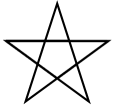
\includegraphics{star.png}
\end{quote}

Hints:
\begin{itemize}
\item {} 
Try this on a piece of paper, moving and turning your cellphone as if it was a
turtle.  Watch how many complete rotations your cellphone makes before you complete the
star.  Since each full rotation is 360 degrees, you can figure out the total
number of degrees that your phone was rotated through.  If you divide that by 5, because
there are five points to the star, you'll know how many degrees to turn the turtle at each point.

\item {} 
You can hide a turtle behind its invisibility cloak if you don't want it shown.  It will still
draw its lines if its pen is down.  The method is invoked as \code{tess.hideturtle()} .  To make the
turtle visible again, use \code{tess.showturtle()} .

\end{itemize}

\item {} 
Write a program to draw a face of a clock that looks something like this:
\begin{quote}

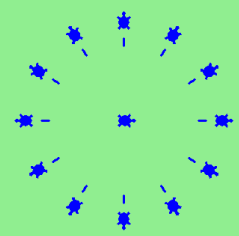
\includegraphics{tess_clock1.png}
\end{quote}

\item {} 
Create a turtle, and assign it to a variable.  When you ask for its type, what do you get?

\item {} 
What is the collective noun for turtles?  (Hint: they don't come in \emph{herds}.)

\item {} 
What the collective noun for pythons?  Is a python a viper?  Is a python venomous?

\end{enumerate}

\begin{DUlineblock}{0em}
\item[] 
\end{DUlineblock}


\chapter{Functions}
\label{functions:functions}\label{functions::doc}
\index{function}\index{function definition}\index{definition!function}

\section{Functions}
\label{functions:index-0}\label{functions:id1}
In Python, a \textbf{function} is a named sequence of statements
that belong together.  Their primary purpose is to help us
organize programs into chunks that match how we think about
the problem.

The syntax for a \textbf{function definition} is:
\begin{quote}

\begin{Verbatim}[commandchars=\\\{\}]
\PYG{k}{def} \PYG{n+nf}{NAME}\PYG{p}{(} \PYG{n}{PARAMETERS} \PYG{p}{)}\PYG{p}{:}
    \PYG{n}{STATEMENTS}
\end{Verbatim}
\end{quote}

We can make up any names we want for the functions we create, except that
we can't use a name that is a Python keyword, and the names must follow the rules
for legal identifiers.

There can be any number of statements inside the function, but they have to be
indented from the \code{def}. In the examples in this book, we will use the
standard indentation of four spaces. Function definitions are the second of
several \textbf{compound statements} we will see, all of which have the same
pattern:
\begin{enumerate}
\item {} 
A header line which begins with a keyword and ends with a colon.

\item {} 
A \textbf{body} consisting of one or more Python statements, each
indented the same amount --- \emph{4 spaces is the Python standard} --- from
the header line.

\end{enumerate}

We've already seen the \code{for} loop which follows this pattern.

So looking again at the function definition, the keyword in the header is \code{def}, which is
followed by the name of the function and some \emph{parameters} enclosed in
parentheses. The parameter list may be empty, or it may contain any number of
parameters separated from one another by commas. In either case, the parentheses are required.
The parameters specifies what information, if any, we have to provide in order to use the new function.

Suppose we're working with turtles, and a common operation we need is to draw
squares.   ``Draw a square'' is an \emph{abstraction}, or a mental
chunk, of a number of smaller steps.  So let's write a function to capture the pattern
of this ``building block'':
\begin{quote}

\begin{Verbatim}[commandchars=\\\{\},numbers=left,firstnumber=1,stepnumber=1]
 \PYG{k+kn}{import} \PYG{n+nn}{turtle}

 \PYG{k}{def} \PYG{n+nf}{draw\PYGZus{}square}\PYG{p}{(}\PYG{n}{t}\PYG{p}{,} \PYG{n}{sz}\PYG{p}{)}\PYG{p}{:}
     \PYG{l+s+sd}{"""Make turtle t draw a square of sz."""}

     \PYG{k}{for} \PYG{n}{i} \PYG{o+ow}{in} \PYG{n+nb}{range}\PYG{p}{(}\PYG{l+m+mi}{4}\PYG{p}{)}\PYG{p}{:}
         \PYG{n}{t}\PYG{o}{.}\PYG{n}{forward}\PYG{p}{(}\PYG{n}{sz}\PYG{p}{)}
         \PYG{n}{t}\PYG{o}{.}\PYG{n}{left}\PYG{p}{(}\PYG{l+m+mi}{90}\PYG{p}{)}


 \PYG{n}{wn} \PYG{o}{=} \PYG{n}{turtle}\PYG{o}{.}\PYG{n}{Screen}\PYG{p}{(}\PYG{p}{)}        \PYG{c}{\PYGZsh{} Set up the window and its attributes}
 \PYG{n}{wn}\PYG{o}{.}\PYG{n}{bgcolor}\PYG{p}{(}\PYG{l+s}{"}\PYG{l+s}{lightgreen}\PYG{l+s}{"}\PYG{p}{)}
 \PYG{n}{wn}\PYG{o}{.}\PYG{n}{title}\PYG{p}{(}\PYG{l+s}{"}\PYG{l+s}{Alex meets a function}\PYG{l+s}{"}\PYG{p}{)}

 \PYG{n}{alex} \PYG{o}{=} \PYG{n}{turtle}\PYG{o}{.}\PYG{n}{Turtle}\PYG{p}{(}\PYG{p}{)}      \PYG{c}{\PYGZsh{} Create alex}
 \PYG{n}{draw\PYGZus{}square}\PYG{p}{(}\PYG{n}{alex}\PYG{p}{,} \PYG{l+m+mi}{50}\PYG{p}{)}       \PYG{c}{\PYGZsh{} Call the function to draw the square}
 \PYG{n}{wn}\PYG{o}{.}\PYG{n}{mainloop}\PYG{p}{(}\PYG{p}{)}
\end{Verbatim}

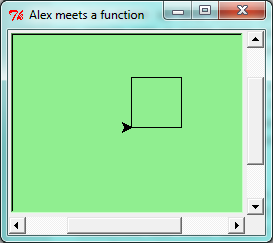
\includegraphics{alex04.png}
\end{quote}

This function is named \code{draw\_square}.  It has two parameters: one to tell
the function which turtle to move around, and the other to tell it the size
of the square we want drawn.   Make sure you know where the body of the function
ends --- it depends on the indentation, and the blank lines don't count for
this purpose!

\begin{notice}{note}{Docstrings for documentation}

If the first thing after the function header is a string, it is
treated as a \textbf{docstring} and gets special treatment in Python and
in some programming tools. For example, when we type a built-in
function name with an unclosed parenthesis in PyScripter, a tooltip
shows up telling us what arguments the function takes, what it does,
and any other text contained in the docstring.

Docstrings are the key way to document our functions in Python and
the documentation part is important. Because whoever calls our
function shouldn't have to need to know what is going on in the
function or how it works; they just need to know what arguments our
function takes, what it does, and what the expected result is.
Enough to be able to use the function without having to look
underneath. This goes back to the concept of abstraction of which
we'll talk more about.

Docstrings are usually formed using triple-quoted strings as they
allow us to easily expand the docstring later on should we want to
write more than a one-liner.

Just to differentiate from comments, a string at the start of a
function (a docstring) is retrievable by Python tools \emph{at runtime}.
By contrast, comments are completely eliminated when the program is
parsed.
\end{notice}

Defining a new function does not make the function run. To do that we need a
\textbf{function call}. We've already seen how to call some built-in functions like
\textbf{print}, \textbf{range} and \textbf{int}. Function calls contain the name of the function being
executed followed by a list of values, called \emph{arguments}, which are assigned
to the parameters in the function definition.  So in the second last line of
the program, we call the function, and pass \code{alex} as the turtle to be manipulated,
and 50 as the size of the square we want. While the function is executing, then, the
variable \code{sz} refers to the value 50, and the variable \code{t} refers to the same
turtle instance that the variable \code{alex} refers to.

Once we've defined a function, we can call it as often as we like, and its
statements will be executed each time we call it.  And we could use it to get
any of our turtles to draw a square.   In the next example, we've changed the \code{draw\_square}
function a little, and we get tess to draw 15 squares, with some variations.
\begin{quote}

\begin{Verbatim}[commandchars=\\\{\},numbers=left,firstnumber=1,stepnumber=1]
\PYG{k+kn}{import} \PYG{n+nn}{turtle}

\PYG{k}{def} \PYG{n+nf}{draw\PYGZus{}multicolor\PYGZus{}square}\PYG{p}{(}\PYG{n}{t}\PYG{p}{,} \PYG{n}{sz}\PYG{p}{)}\PYG{p}{:}
    \PYG{l+s+sd}{"""Make turtle t draw a multi-color square of sz."""}
    \PYG{k}{for} \PYG{n}{i} \PYG{o+ow}{in} \PYG{p}{[}\PYG{l+s}{"}\PYG{l+s}{red}\PYG{l+s}{"}\PYG{p}{,} \PYG{l+s}{"}\PYG{l+s}{purple}\PYG{l+s}{"}\PYG{p}{,} \PYG{l+s}{"}\PYG{l+s}{hotpink}\PYG{l+s}{"}\PYG{p}{,} \PYG{l+s}{"}\PYG{l+s}{blue}\PYG{l+s}{"}\PYG{p}{]}\PYG{p}{:}
        \PYG{n}{t}\PYG{o}{.}\PYG{n}{color}\PYG{p}{(}\PYG{n}{i}\PYG{p}{)}
        \PYG{n}{t}\PYG{o}{.}\PYG{n}{forward}\PYG{p}{(}\PYG{n}{sz}\PYG{p}{)}
        \PYG{n}{t}\PYG{o}{.}\PYG{n}{left}\PYG{p}{(}\PYG{l+m+mi}{90}\PYG{p}{)}

\PYG{n}{wn} \PYG{o}{=} \PYG{n}{turtle}\PYG{o}{.}\PYG{n}{Screen}\PYG{p}{(}\PYG{p}{)}        \PYG{c}{\PYGZsh{} Set up the window and its attributes}
\PYG{n}{wn}\PYG{o}{.}\PYG{n}{bgcolor}\PYG{p}{(}\PYG{l+s}{"}\PYG{l+s}{lightgreen}\PYG{l+s}{"}\PYG{p}{)}

\PYG{n}{tess} \PYG{o}{=} \PYG{n}{turtle}\PYG{o}{.}\PYG{n}{Turtle}\PYG{p}{(}\PYG{p}{)}      \PYG{c}{\PYGZsh{} Create tess and set some attributes}
\PYG{n}{tess}\PYG{o}{.}\PYG{n}{pensize}\PYG{p}{(}\PYG{l+m+mi}{3}\PYG{p}{)}

\PYG{n}{size} \PYG{o}{=} \PYG{l+m+mi}{20}                   \PYG{c}{\PYGZsh{} Size of the smallest square}
\PYG{k}{for} \PYG{n}{i} \PYG{o+ow}{in} \PYG{n+nb}{range}\PYG{p}{(}\PYG{l+m+mi}{15}\PYG{p}{)}\PYG{p}{:}
    \PYG{n}{draw\PYGZus{}multicolor\PYGZus{}square}\PYG{p}{(}\PYG{n}{tess}\PYG{p}{,} \PYG{n}{size}\PYG{p}{)}
    \PYG{n}{size} \PYG{o}{=} \PYG{n}{size} \PYG{o}{+} \PYG{l+m+mi}{10}        \PYG{c}{\PYGZsh{} Increase the size for next time}
    \PYG{n}{tess}\PYG{o}{.}\PYG{n}{forward}\PYG{p}{(}\PYG{l+m+mi}{10}\PYG{p}{)}        \PYG{c}{\PYGZsh{} Move tess along a little}
    \PYG{n}{tess}\PYG{o}{.}\PYG{n}{right}\PYG{p}{(}\PYG{l+m+mi}{18}\PYG{p}{)}          \PYG{c}{\PYGZsh{}    and give her some extra turn}

\PYG{n}{wn}\PYG{o}{.}\PYG{n}{mainloop}\PYG{p}{(}\PYG{p}{)}
\end{Verbatim}

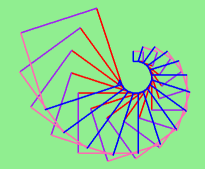
\includegraphics{tess05.png}
\end{quote}


\section{Functions can call other functions}
\label{functions:functions-can-call-other-functions}
Let's assume now we want a function to draw a rectangle.  We need to be able to call
the function with different arguments for width and height.  And, unlike the case of the
square, we cannot repeat the same thing 4 times, because the four sides are not equal.

So we eventually come up with this rather nice code that can draw a rectangle.
\begin{quote}

\begin{Verbatim}[commandchars=\\\{\},numbers=left,firstnumber=1,stepnumber=1]
\PYG{k}{def} \PYG{n+nf}{draw\PYGZus{}rectangle}\PYG{p}{(}\PYG{n}{t}\PYG{p}{,} \PYG{n}{w}\PYG{p}{,} \PYG{n}{h}\PYG{p}{)}\PYG{p}{:}
    \PYG{l+s+sd}{"""Get turtle t to draw a rectangle of width w and height h."""}
    \PYG{k}{for} \PYG{n}{i} \PYG{o+ow}{in} \PYG{n+nb}{range}\PYG{p}{(}\PYG{l+m+mi}{2}\PYG{p}{)}\PYG{p}{:}
        \PYG{n}{t}\PYG{o}{.}\PYG{n}{forward}\PYG{p}{(}\PYG{n}{w}\PYG{p}{)}
        \PYG{n}{t}\PYG{o}{.}\PYG{n}{left}\PYG{p}{(}\PYG{l+m+mi}{90}\PYG{p}{)}
        \PYG{n}{t}\PYG{o}{.}\PYG{n}{forward}\PYG{p}{(}\PYG{n}{h}\PYG{p}{)}
        \PYG{n}{t}\PYG{o}{.}\PYG{n}{left}\PYG{p}{(}\PYG{l+m+mi}{90}\PYG{p}{)}
\end{Verbatim}
\end{quote}

The parameter names are deliberately chosen as single letters to ensure they're not misunderstood.
In real programs, once we've had more experience, we will insist on better variable names than this.
But the point is that the program doesn't ``understand'' that we're drawing a rectangle, or that the
parameters represent the width and the height.  Concepts like rectangle, width, and height are
the meaning we humans have, not concepts that the program or the computer understands.

\emph{Thinking like a scientist} involves looking for patterns and
relationships.  In the code above, we've done that to some extent.  We did not just draw four sides.
Instead, we spotted that we could draw the rectangle as two halves, and used a loop to
repeat that pattern twice.

But now we might spot that a square is a special kind of rectangle.
We already have a function that draws a rectangle, so we can use that to draw
our square.
\begin{quote}

\begin{Verbatim}[commandchars=\\\{\},numbers=left,firstnumber=1,stepnumber=1]
\PYG{k}{def} \PYG{n+nf}{draw\PYGZus{}square}\PYG{p}{(}\PYG{n}{tx}\PYG{p}{,} \PYG{n}{sz}\PYG{p}{)}\PYG{p}{:}        \PYG{c}{\PYGZsh{} A new version of draw\PYGZus{}square}
    \PYG{n}{draw\PYGZus{}rectangle}\PYG{p}{(}\PYG{n}{tx}\PYG{p}{,} \PYG{n}{sz}\PYG{p}{,} \PYG{n}{sz}\PYG{p}{)}
\end{Verbatim}
\end{quote}

There are some points worth noting here:
\begin{itemize}
\item {} 
Functions can call other functions.

\item {} 
Rewriting \code{draw\_square} like this captures the relationship
that we've spotted between squares and rectangles.

\item {} 
A caller of this function might say \code{draw\_square(tess, 50)}.  The parameters
of this function, \code{tx} and \code{sz}, are assigned the values of the tess object, and
the int 50 respectively.

\item {} 
In the body of the function they are just like any other variable.

\item {} 
When the call is made to \code{draw\_rectangle}, the values in variables \code{tx} and \code{sz}
are fetched first, then the call happens.  So as we enter the top of
function \code{draw\_rectangle}, its variable \code{t} is assigned the tess object, and \code{w} and
\code{h} in that function are both given the value 50.

\end{itemize}

So far, it may not be clear why it is worth the trouble to create all of these
new functions. Actually, there are a lot of reasons, but this example
demonstrates two:
\begin{enumerate}
\item {} 
Creating a new function gives us an opportunity to name a group of
statements. Functions can simplify a program by hiding a complex computation
behind a single command. The function (including its name) can capture our
mental chunking, or \emph{abstraction}, of the problem.

\item {} 
Creating a new function can make a program smaller by eliminating repetitive
code.

\end{enumerate}

As we might expect, we have to create a function before we can execute it.
In other words, the function definition has to be executed before the
function is called.

\index{flow of execution}

\section{Flow of execution}
\label{functions:index-1}\label{functions:flow-of-execution}
In order to ensure that a function is defined before its first use, we have to
know the order in which statements are executed, which is called the \textbf{flow of
execution}.   We've already talked about this a little in the previous chapter.

Execution always begins at the first statement of the program.  Statements are
executed one at a time, in order from top to bottom.

Function definitions do not alter the flow of execution of the program, but
remember that statements inside the function are not executed until the
function is called. Although it is not common, we can define one function
inside another. In this case, the inner definition isn't executed until the
outer function is called.

Function calls are like a detour in the flow of execution. Instead of going to
the next statement, the flow jumps to the first line of the called function,
executes all the statements there, and then comes back to pick up where it left
off.

That sounds simple enough, until we remember that one function can call
another. While in the middle of one function, the program might have to execute
the statements in another function. But while executing that new function, the
program might have to execute yet another function!

Fortunately, Python is adept at keeping track of where it is, so each time a
function completes, the program picks up where it left off in the function that
called it. When it gets to the end of the program, it terminates.

What's the moral of this sordid tale? When we read a program, don't read from
top to bottom. Instead, follow the flow of execution.

\index{PyScripter!single stepping}
\begin{notice}{note}{Watch the flow of execution in action}

In PyScripter, we can watch the flow of execution by ``single-stepping'' through
any program.  PyScripter will highlight each line of code just before it is about to
be executed.

PyScripter also lets us hover the mouse over any
variable in the program, and it will pop up the current value of that variable.
So this makes it easy to inspect the ``state snapshot'' of the program --- the
current values that are assigned to the program's variables.

This is a powerful mechanism for building a deep and thorough understanding of
what is happening at each step of the way.  Learn to use the single-stepping
feature well, and be mentally proactive:  as you work through the code,
challenge yourself before each step: \emph{``What changes will this line make to
any variables in the program?''} and \emph{``Where will flow of execution go next?''}

Let us go back and see how this works with the program above that draws 15
multicolor squares.  First, we're going to add one line of magic below
the import statement --- not strictly necessary, but it will make our lives
much simpler, because it prevents stepping into the module containing
the turtle code.
\begin{quote}

\begin{Verbatim}[commandchars=\\\{\}]
\PYG{k+kn}{import} \PYG{n+nn}{turtle}
\PYG{n+nb}{\PYGZus{}\PYGZus{}import\PYGZus{}\PYGZus{}}\PYG{p}{(}\PYG{l+s}{"}\PYG{l+s}{turtle}\PYG{l+s}{"}\PYG{p}{)}\PYG{o}{.}\PYG{n}{\PYGZus{}\PYGZus{}traceable\PYGZus{}\PYGZus{}} \PYG{o}{=} \PYG{k}{False}
\end{Verbatim}
\end{quote}

Now we're ready to begin.  Put the mouse cursor on the line of the program
where we create the turtle screen, and press the \emph{F4} key.  This will run the Python
program up to, but not including, the line where we have the cursor.   Our program
will ``break'' now, and provide a highlight on the next line to be executed, something like this:

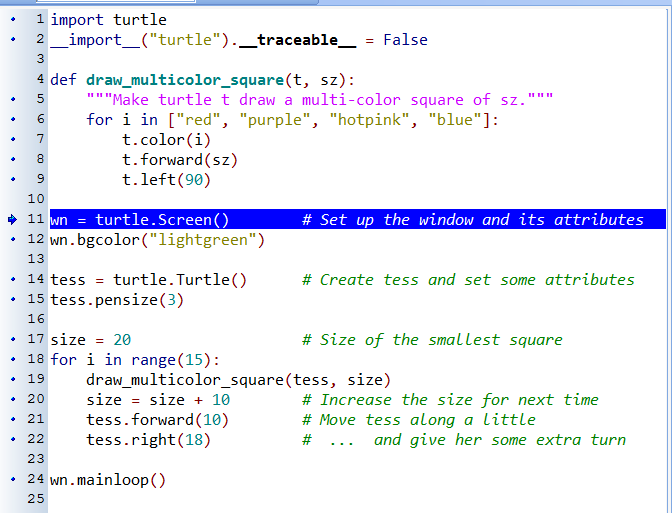
\includegraphics{breakpoint.png}

At this point we can press the \emph{F7} key (\emph{step into}) repeatedly to single step through
the code.  Observe as we execute lines 10, 11, 12, ... how the turtle window gets
created, how its canvas color is changed, how the title
gets changed, how the turtle is created on the canvas, and then how the flow of execution gets into the loop, and from there into the function,
and into the function's loop, and then repeatedly through the body of that loop.

While we do this, we can also hover our mouse over some of the variables in the program, and confirm that
their values match our conceptual model of what is happening.

After a few loops, when we're about to execute line 20 and we're starting to get bored, we can use the key \emph{F8}
to ``step over'' the function we are calling.  This executes all the statements in the function, but without
having to step through each one.   We always have the choice to either
``go for the detail'', or to ``take the high-level view'' and execute the function as a single chunk.

There are some other options, including one that allow us to \emph{resume} execution without further stepping.
Find them under the \emph{Run} menu of PyScripter.
\end{notice}

\index{parameter}\index{function!parameter}\index{argument}\index{function!argument}\index{import statement}\index{statement!import}\index{composition}\index{function!composition}

\section{Functions that require arugments}
\label{functions:functions-that-require-arugments}\label{functions:index-3}
Most functions require arguments: the arguments provide for generalization.
For example, if we want to find the absolute value of a number, we have
to indicate what the number is. Python has a built-in function for
computing the absolute value:
\begin{quote}

\begin{Verbatim}[commandchars=\\\{\}]
\PYG{g+gp}{\PYGZgt{}\PYGZgt{}\PYGZgt{} }\PYG{n+nb}{abs}\PYG{p}{(}\PYG{l+m+mi}{5}\PYG{p}{)}
\PYG{g+go}{5}
\PYG{g+gp}{\PYGZgt{}\PYGZgt{}\PYGZgt{} }\PYG{n+nb}{abs}\PYG{p}{(}\PYG{o}{-}\PYG{l+m+mi}{5}\PYG{p}{)}
\PYG{g+go}{5}
\end{Verbatim}
\end{quote}

In this example, the arguments to the \code{abs} function are 5 and -5.

Some functions take more than one argument. For example the built-in function
\code{pow} takes two arguments, the base and the exponent. Inside the function,
the values that are passed get assigned to variables called \textbf{parameters}.
\begin{quote}

\begin{Verbatim}[commandchars=\\\{\}]
\PYG{g+gp}{\PYGZgt{}\PYGZgt{}\PYGZgt{} }\PYG{n+nb}{pow}\PYG{p}{(}\PYG{l+m+mi}{2}\PYG{p}{,} \PYG{l+m+mi}{3}\PYG{p}{)}
\PYG{g+go}{8}
\PYG{g+gp}{\PYGZgt{}\PYGZgt{}\PYGZgt{} }\PYG{n+nb}{pow}\PYG{p}{(}\PYG{l+m+mi}{7}\PYG{p}{,} \PYG{l+m+mi}{4}\PYG{p}{)}
\PYG{g+go}{2401}
\end{Verbatim}
\end{quote}

Another built-in function that takes more than one argument is \code{max}.
\begin{quote}

\begin{Verbatim}[commandchars=\\\{\}]
\PYG{g+gp}{\PYGZgt{}\PYGZgt{}\PYGZgt{} }\PYG{n+nb}{max}\PYG{p}{(}\PYG{l+m+mi}{7}\PYG{p}{,} \PYG{l+m+mi}{11}\PYG{p}{)}
\PYG{g+go}{11}
\PYG{g+gp}{\PYGZgt{}\PYGZgt{}\PYGZgt{} }\PYG{n+nb}{max}\PYG{p}{(}\PYG{l+m+mi}{4}\PYG{p}{,} \PYG{l+m+mi}{1}\PYG{p}{,} \PYG{l+m+mi}{17}\PYG{p}{,} \PYG{l+m+mi}{2}\PYG{p}{,} \PYG{l+m+mi}{12}\PYG{p}{)}
\PYG{g+go}{17}
\PYG{g+gp}{\PYGZgt{}\PYGZgt{}\PYGZgt{} }\PYG{n+nb}{max}\PYG{p}{(}\PYG{l+m+mi}{3} \PYG{o}{*} \PYG{l+m+mi}{11}\PYG{p}{,} \PYG{l+m+mi}{5}\PYG{o}{*}\PYG{o}{*}\PYG{l+m+mi}{3}\PYG{p}{,} \PYG{l+m+mi}{512} \PYG{o}{-} \PYG{l+m+mi}{9}\PYG{p}{,} \PYG{l+m+mi}{1024}\PYG{o}{*}\PYG{o}{*}\PYG{l+m+mi}{0}\PYG{p}{)}
\PYG{g+go}{503}
\end{Verbatim}
\end{quote}

\code{max} can be passed any number of arguments, separated by commas, and will
return the largest value passed. The arguments can be either simple values or
expressions. In the last example, 503 is returned, since it is larger than 33,
125, and 1.


\section{Functions that return values}
\label{functions:functions-that-return-values}
All the functions in the previous section return values.
Furthermore, functions like \code{range}, \code{int}, \code{abs} all return values that
can be used to build more complex expressions.

So an important difference between these functions and one like \code{draw\_square} is that
\code{draw\_square} was not executed because we wanted it to compute a value --- on the contrary,
we wrote \code{draw\_square} because we wanted it to execute a sequence of steps that caused
the turtle to draw.

A function that returns a value is called a \textbf{fruitful function} in this book.
The opposite of a fruitful function is \textbf{void function} --- one that is not executed
for its resulting value, but is executed because it does something useful. (Languages
like Java, C\#, C and C++ use the term ``void function'', other languages like Pascal
call it a \textbf{procedure}.) Even though void functions are not executed
for their resulting value, Python always wants to return something.  So if the programmer
doesn't arrange to return a value, Python will automatically return the value \code{None}.

How do we write our own fruitful function?  In the exercises at the end of chapter 2 we saw
the standard formula for compound interest, which we'll now write as a fruitful function:
\begin{quote}

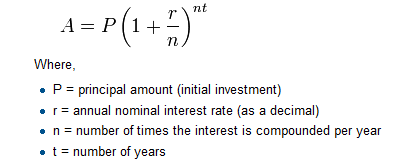
\includegraphics{compoundInterest.png}

\begin{Verbatim}[commandchars=\\\{\},numbers=left,firstnumber=1,stepnumber=1]
\PYG{k}{def} \PYG{n+nf}{final\PYGZus{}amt}\PYG{p}{(}\PYG{n}{p}\PYG{p}{,} \PYG{n}{r}\PYG{p}{,} \PYG{n}{n}\PYG{p}{,} \PYG{n}{t}\PYG{p}{)}\PYG{p}{:}
    \PYG{l+s+sd}{"""}
\PYG{l+s+sd}{      Apply the compound interest formula to p}
\PYG{l+s+sd}{       to produce the final amount.}
\PYG{l+s+sd}{    """}

    \PYG{n}{a} \PYG{o}{=} \PYG{n}{p} \PYG{o}{*} \PYG{p}{(}\PYG{l+m+mi}{1} \PYG{o}{+} \PYG{n}{r}\PYG{o}{/}\PYG{n}{n}\PYG{p}{)} \PYG{o}{*}\PYG{o}{*} \PYG{p}{(}\PYG{n}{n}\PYG{o}{*}\PYG{n}{t}\PYG{p}{)}
    \PYG{k}{return} \PYG{n}{a}         \PYG{c}{\PYGZsh{} This is new, and makes the function fruitful.}

\PYG{c}{\PYGZsh{} now that we have the function above, let us call it.}
\PYG{n}{toInvest} \PYG{o}{=} \PYG{n+nb}{float}\PYG{p}{(}\PYG{n+nb}{input}\PYG{p}{(}\PYG{l+s}{"}\PYG{l+s}{How much do you want to invest?}\PYG{l+s}{"}\PYG{p}{)}\PYG{p}{)}
\PYG{n}{fnl} \PYG{o}{=} \PYG{n}{final\PYGZus{}amt}\PYG{p}{(}\PYG{n}{toInvest}\PYG{p}{,} \PYG{l+m+mf}{0.08}\PYG{p}{,} \PYG{l+m+mi}{12}\PYG{p}{,} \PYG{l+m+mi}{5}\PYG{p}{)}
\PYG{n+nb}{print}\PYG{p}{(}\PYG{l+s}{"}\PYG{l+s}{At the end of the period you}\PYG{l+s}{'}\PYG{l+s}{ll have}\PYG{l+s}{"}\PYG{p}{,} \PYG{n}{fnl}\PYG{p}{)}
\end{Verbatim}
\end{quote}
\begin{itemize}
\item {} 
The \textbf{return} statement is followed an expression (\code{a} in this case). This expression will be
evaluated and returned to the caller as the ``fruit'' of calling this function.

\item {} 
We prompted the user for the principal amount.  The type of \code{toInvest} is a string, but
we need a number before we can work with it.  Because it is money, and could have decimal places,
we've used the \code{float} type converter function to parse the string and return a float.

\item {} 
Notice how we entered the arguments for 8\% interest, compounded 12 times per year, for 5 years.

\item {} 
When we run this, we get the output
\begin{quote}

\emph{At the end of the period you'll have 14898.457083}
\end{quote}

This is a bit messy with all these decimal places, but remember that
Python doesn't understand that we're working with money: it just does the calculation to
the best of its ability, without rounding.  Later we'll see how to format the string that
is printed in such a way that it does get nicely rounded to two decimal places before printing.

\item {} 
The line \code{toInvest = float(input("How much do you want to invest?"))}
also shows yet another example
of \emph{composition} --- we can call a function like \code{float}, and its arguments
can be the results of other function calls (like \code{input}) that we've called along the way.

\end{itemize}

Notice something else very important here. The name of the variable we pass as an
argument --- \code{toInvest} --- has nothing to do with the name of the parameter
--- \code{p}.  It is as if  \code{p = toInvest} is executed when \code{final\_amt} is called.
It doesn't matter what the value was named in
the caller, in \code{final\_amt} its name is \code{p}.

These short variable names are getting quite tricky, so perhaps we'd prefer one of these
versions instead:
\begin{quote}

\begin{Verbatim}[commandchars=\\\{\},numbers=left,firstnumber=1,stepnumber=1]
\PYG{k}{def} \PYG{n+nf}{final\PYGZus{}amt\PYGZus{}v2}\PYG{p}{(}\PYG{n}{principalAmount}\PYG{p}{,} \PYG{n}{nominalPercentageRate}\PYG{p}{,}
                                    \PYG{n}{numTimesPerYear}\PYG{p}{,} \PYG{n}{years}\PYG{p}{)}\PYG{p}{:}
    \PYG{n}{a} \PYG{o}{=} \PYG{n}{principalAmount} \PYG{o}{*} \PYG{p}{(}\PYG{l+m+mi}{1} \PYG{o}{+} \PYG{n}{nominalPercentageRate} \PYG{o}{/}
                         \PYG{n}{numTimesPerYear}\PYG{p}{)} \PYG{o}{*}\PYG{o}{*} \PYG{p}{(}\PYG{n}{numTimesPerYear}\PYG{o}{*}\PYG{n}{years}\PYG{p}{)}
    \PYG{k}{return} \PYG{n}{a}

\PYG{k}{def} \PYG{n+nf}{final\PYGZus{}amt\PYGZus{}v3}\PYG{p}{(}\PYG{n}{amt}\PYG{p}{,} \PYG{n}{rate}\PYG{p}{,} \PYG{n}{compounded}\PYG{p}{,} \PYG{n}{years}\PYG{p}{)}\PYG{p}{:}
    \PYG{n}{a} \PYG{o}{=} \PYG{n}{amt} \PYG{o}{*} \PYG{p}{(}\PYG{l+m+mi}{1} \PYG{o}{+} \PYG{n}{rate}\PYG{o}{/}\PYG{n}{compounded}\PYG{p}{)} \PYG{o}{*}\PYG{o}{*} \PYG{p}{(}\PYG{n}{componded}\PYG{o}{*}\PYG{n}{years}\PYG{p}{)}
    \PYG{k}{return} \PYG{n}{a}
\end{Verbatim}
\end{quote}

They all do the same thing.   Use your judgement to write code that can be best
understood by other humans!
Short variable names are more economical and sometimes make
code easier to read:
E = mc$^{\text{2}}$ would not be nearly so memorable if Einstein had
used longer variable names!  If you do prefer short names,
make sure you also have some comments to enlighten the reader
about what the variables are used for.

\index{local variable}\index{variable!local}\index{lifetime}

\section{Variables and parameters are local}
\label{functions:index-4}\label{functions:variables-and-parameters-are-local}
When we create a \textbf{local variable} inside a function, it only exists inside
the function, and we cannot use it outside. For example, consider again this function:
\begin{quote}

\begin{Verbatim}[commandchars=\\\{\},numbers=left,firstnumber=1,stepnumber=1]
\PYG{k}{def} \PYG{n+nf}{final\PYGZus{}amt}\PYG{p}{(}\PYG{n}{p}\PYG{p}{,} \PYG{n}{r}\PYG{p}{,} \PYG{n}{n}\PYG{p}{,} \PYG{n}{t}\PYG{p}{)}\PYG{p}{:}
    \PYG{n}{a} \PYG{o}{=} \PYG{n}{p} \PYG{o}{*} \PYG{p}{(}\PYG{l+m+mi}{1} \PYG{o}{+} \PYG{n}{r}\PYG{o}{/}\PYG{n}{n}\PYG{p}{)} \PYG{o}{*}\PYG{o}{*} \PYG{p}{(}\PYG{n}{n}\PYG{o}{*}\PYG{n}{t}\PYG{p}{)}
    \PYG{k}{return} \PYG{n}{a}
\end{Verbatim}
\end{quote}

If we try to use \code{a}, outside the function, we'll get an error:
\begin{quote}

\begin{Verbatim}[commandchars=\\\{\}]
\PYG{g+gp}{\PYGZgt{}\PYGZgt{}\PYGZgt{} }\PYG{n}{a}
\PYG{g+go}{NameError: name 'a' is not defined}
\end{Verbatim}
\end{quote}

The variable \code{a} is local to \code{final\_amt}, and is not visible
outside the function.

Additionally, \code{a} only exists while the function is being executed ---
we call this its \textbf{lifetime}.
When the execution of the function terminates,
the local variables  are destroyed.

Parameters are also local, and act like local variables.
For example, the lifetimes of \code{p}, \code{r}, \code{n}, \code{t} begin when \code{final\_amt} is called,
and the lifetime ends when the function completes its execution.

So it is not possible for a function to set some local variable to a
value, complete its execution, and then when it is called again next
time, recover the local variable.  Each call of the function creates
new local variables, and their lifetimes expire when the function returns
to the caller.

\index{refactoring code}\index{chunking}

\section{Turtles Revisited}
\label{functions:turtles-revisited}\label{functions:index-5}
Now that we have fruitful functions, we can focus our attention on
reorganizing our code so that it fits more nicely into our mental chunks.
This process of rearrangement is called \textbf{refactoring} the code.

Two things we're always going to want to do when working with turtles
is to create the window for the turtle, and to create one or more turtles.
We could write some functions to make these tasks easier in future:
\begin{quote}

\begin{Verbatim}[commandchars=\\\{\},numbers=left,firstnumber=1,stepnumber=1]
\PYG{k}{def} \PYG{n+nf}{make\PYGZus{}window}\PYG{p}{(}\PYG{n}{colr}\PYG{p}{,} \PYG{n}{ttle}\PYG{p}{)}\PYG{p}{:}
    \PYG{l+s+sd}{"""}
\PYG{l+s+sd}{      Set up the window with the given background color and title.}
\PYG{l+s+sd}{      Returns the new window.}
\PYG{l+s+sd}{    """}
    \PYG{n}{w} \PYG{o}{=} \PYG{n}{turtle}\PYG{o}{.}\PYG{n}{Screen}\PYG{p}{(}\PYG{p}{)}
    \PYG{n}{w}\PYG{o}{.}\PYG{n}{bgcolor}\PYG{p}{(}\PYG{n}{colr}\PYG{p}{)}
    \PYG{n}{w}\PYG{o}{.}\PYG{n}{title}\PYG{p}{(}\PYG{n}{ttle}\PYG{p}{)}
    \PYG{k}{return} \PYG{n}{w}


\PYG{k}{def} \PYG{n+nf}{make\PYGZus{}turtle}\PYG{p}{(}\PYG{n}{colr}\PYG{p}{,} \PYG{n}{sz}\PYG{p}{)}\PYG{p}{:}
    \PYG{l+s+sd}{"""}
\PYG{l+s+sd}{      Set up a turtle with the given color and pensize.}
\PYG{l+s+sd}{      Returns the new turtle.}
\PYG{l+s+sd}{    """}
    \PYG{n}{t} \PYG{o}{=} \PYG{n}{turtle}\PYG{o}{.}\PYG{n}{Turtle}\PYG{p}{(}\PYG{p}{)}
    \PYG{n}{t}\PYG{o}{.}\PYG{n}{color}\PYG{p}{(}\PYG{n}{colr}\PYG{p}{)}
    \PYG{n}{t}\PYG{o}{.}\PYG{n}{pensize}\PYG{p}{(}\PYG{n}{sz}\PYG{p}{)}
    \PYG{k}{return} \PYG{n}{t}


\PYG{n}{wn} \PYG{o}{=} \PYG{n}{make\PYGZus{}window}\PYG{p}{(}\PYG{l+s}{"}\PYG{l+s}{lightgreen}\PYG{l+s}{"}\PYG{p}{,} \PYG{l+s}{"}\PYG{l+s}{Tess and Alex dancing}\PYG{l+s}{"}\PYG{p}{)}
\PYG{n}{tess} \PYG{o}{=} \PYG{n}{make\PYGZus{}turtle}\PYG{p}{(}\PYG{l+s}{"}\PYG{l+s}{hotpink}\PYG{l+s}{"}\PYG{p}{,} \PYG{l+m+mi}{5}\PYG{p}{)}
\PYG{n}{alex} \PYG{o}{=} \PYG{n}{make\PYGZus{}turtle}\PYG{p}{(}\PYG{l+s}{"}\PYG{l+s}{black}\PYG{l+s}{"}\PYG{p}{,} \PYG{l+m+mi}{1}\PYG{p}{)}
\PYG{n}{dave} \PYG{o}{=} \PYG{n}{make\PYGZus{}turtle}\PYG{p}{(}\PYG{l+s}{"}\PYG{l+s}{yellow}\PYG{l+s}{"}\PYG{p}{,} \PYG{l+m+mi}{2}\PYG{p}{)}
\end{Verbatim}
\end{quote}

The trick about refactoring code is to anticipate which things we are likely to want to change
each time we call the function: these should become the parameters, or changeable p,
of the functions we write.


\section{Glossary}
\label{functions:glossary}\begin{description}
\item[{\index{argument|textbf}argument}] \leavevmode\phantomsection\label{functions:term-argument}
A value provided to a function when the function is called. This value
is assigned to the corresponding parameter in the function.  The argument
can be the result of an expression which may involve operators,
operands and calls to other fruitful functions.

\item[{\index{body|textbf}body}] \leavevmode\phantomsection\label{functions:term-body}
The second part of a compound statement. The body consists of a
sequence of statements all indented the same amount from the beginning
of the header.  The standard amount of indentation used within the
Python community is 4 spaces.

\item[{\index{compound statement|textbf}compound statement}] \leavevmode\phantomsection\label{functions:term-compound-statement}
A statement that consists of two parts:
\begin{enumerate}
\item {} 
header - which begins with a keyword determining the statement
type, and ends with a colon.

\item {} 
body - containing one or more statements indented the same amount
from the header.

\end{enumerate}

The syntax of a compound statement looks like this:
\begin{quote}

\begin{Verbatim}[commandchars=\\\{\}]
\PYG{n}{keyword} \PYG{n}{expression}\PYG{p}{:}
    \PYG{n}{statement}
    \PYG{n}{statement} \PYG{o}{.}\PYG{o}{.}\PYG{o}{.}
\end{Verbatim}
\end{quote}

\item[{\index{docstring|textbf}docstring}] \leavevmode\phantomsection\label{functions:term-docstring}
If the first thing in a function body is a string (or, we'll see later, in other situations
too) that is attached to the function as its \code{\_\_doc\_\_} attribute,
and can be used by tools like PyScripter.

\item[{\index{flow of execution|textbf}flow of execution}] \leavevmode\phantomsection\label{functions:term-flow-of-execution}
The order in which statements are executed during a program run.

\item[{\index{frame|textbf}frame}] \leavevmode\phantomsection\label{functions:term-frame}
A box in a stack diagram that represents a function call. It contains
the local variables and parameters of the function.

\item[{\index{function|textbf}function}] \leavevmode\phantomsection\label{functions:term-function}
A named sequence of statements that performs some useful operation.
Functions may or may not take parameters and may or may not produce a
result.

\item[{\index{function call|textbf}function call}] \leavevmode\phantomsection\label{functions:term-function-call}
A statement that executes a function. It consists of the name of the
function followed by a list of arguments enclosed in parentheses.

\item[{\index{function composition|textbf}function composition}] \leavevmode\phantomsection\label{functions:term-function-composition}
Using the output from one function call as the input to another.

\item[{\index{function definition|textbf}function definition}] \leavevmode\phantomsection\label{functions:term-function-definition}
A statement that creates a new function, specifying its name,
parameters, and the statements it executes.

\item[{\index{fruitful function|textbf}fruitful function}] \leavevmode\phantomsection\label{functions:term-fruitful-function}
A function that returns a value when it is called.

\item[{\index{header line|textbf}header line}] \leavevmode\phantomsection\label{functions:term-header-line}
The first part of a compound statement. A header line begins with a keyword and
ends with a colon (:)

\item[{\index{import statement|textbf}import statement}] \leavevmode\phantomsection\label{functions:term-import-statement}
A statement which permits functions and variables defined in another Python
module to be brought into the environment of another script.  To use the
features of the turtle, we need to first import the turtle module.

\item[{\index{lifetime|textbf}lifetime}] \leavevmode\phantomsection\label{functions:term-lifetime}
Variables and objects have lifetimes --- they are created at some point during
program execution, and will be destroyed at some time.

\item[{\index{local variable|textbf}local variable}] \leavevmode\phantomsection\label{functions:term-local-variable}
A variable defined inside a function. A local variable can only be used
inside its function.  Parameters of a function are also a special kind
of local variable.

\item[{\index{parameter|textbf}parameter}] \leavevmode\phantomsection\label{functions:term-parameter}
A name used inside a function to refer to the value which was passed
to it as an argument.

\item[{\index{refactor|textbf}refactor}] \leavevmode\phantomsection\label{functions:term-refactor}
A fancy word to describe reorganizing our program code, usually to make
it more understandable.  Typically, we have a program that is already working,
then we go back to ``tidy it up''.  It often involves choosing better variable
names, or spotting repeated patterns and moving that code into a function.

\item[{\index{stack diagram|textbf}stack diagram}] \leavevmode\phantomsection\label{functions:term-stack-diagram}
A graphical representation of a stack of functions, their variables,
and the values to which they refer.

\item[{\index{traceback|textbf}traceback}] \leavevmode\phantomsection\label{functions:term-traceback}
A list of the functions that are executing, printed when a runtime
error occurs. A traceback is also commonly refered to as a
\emph{stack trace}, since it lists the functions in the order in which they
are stored in the
\href{http://en.wikipedia.org/wiki/Runtime\_stack}{runtime stack}.

\item[{\index{void function|textbf}void function}] \leavevmode\phantomsection\label{functions:term-void-function}
The opposite of a fruitful function: one that does not return a value.  It is
executed for the work it does, rather than for the value it returns.

\end{description}


\section{Exercises}
\label{functions:exercises}\begin{enumerate}
\item {} 
Write a void (non-fruitful) function to draw a square.  Use it in a program to draw the image shown below.
Assume each side is 20 units.
(Hint: notice that the turtle has already moved away from the ending point of the last
square when the program ends.)

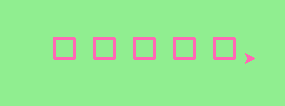
\includegraphics{five_squares.png}

\item {} 
Write a program to draw this. Assume the innermost square is 20 units per side,
and each successive square is 20 units bigger, per side, than the one inside it.

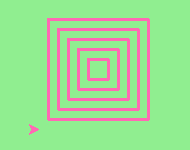
\includegraphics{nested_squares.png}

\item {} 
Write a void function \code{draw\_poly(t, n, sz)} which makes a turtle
draw a regular polygon.
When called with \code{draw\_poly(tess, 8, 50)}, it will draw a shape like this:

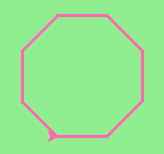
\includegraphics{regularpolygon.png}

\item {} 
Draw this pretty pattern.

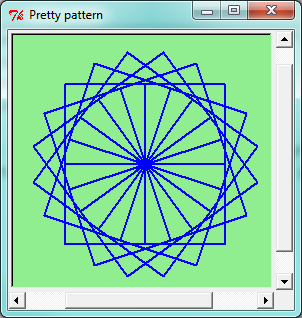
\includegraphics{tess08.png}

\item {} 
The two spirals in this picture differ only by the turn angle.  Draw both.

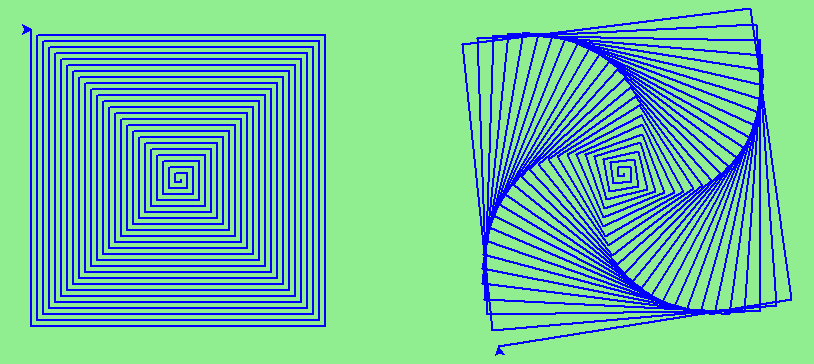
\includegraphics{tess_spirals.png}

\item {} 
Write a void function \code{draw\_equitriangle(t, sz)} which calls \code{draw\_poly} from the
previous question to have its turtle draw a equilateral triangle.

\item {} 
Write a fruitful function \code{sum\_to(n)} that returns the sum of all integer numbers up to and
including \code{n}.   So \code{sum\_to(10)} would be \emph{1+2+3...+10} which would return the value 55.

\item {} 
Write a function \code{area\_of\_circle(r)} which returns the area of a circle of radius \code{r}.

\item {} 
Write a void function to draw a star, where the length of each side is 100 units.
(Hint: You should turn the turtle by 144 degrees at each point.)
\begin{quote}

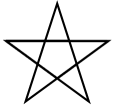
\includegraphics{star.png}
\end{quote}

\item {} 
Extend your program above.  Draw five stars, but between each, pick up the pen,
move forward by 350 units, turn right by 144, put the pen down, and draw the next star.
You'll get something like this:

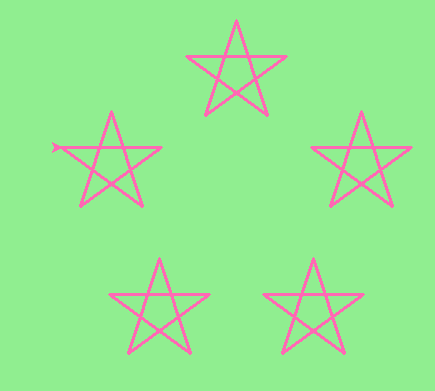
\includegraphics{five_stars.png}

What would it look like if you didn't pick up the pen?

\end{enumerate}

\begin{DUlineblock}{0em}
\item[] 
\end{DUlineblock}


\chapter{Conditionals}
\label{conditionals::doc}\label{conditionals:conditionals}
Programs get really interesting when we can test conditions and change the
program behaviour depending on the outcome of the tests.  That's what this
chapter is about.

\index{Boolean value}\index{value!Boolean}\index{Boolean expression}\index{expression!Boolean}\index{logical operator}\index{operator!logical}\index{operator!comparison}\index{comparison operator}

\section{Boolean values and expressions}
\label{conditionals:index-0}\label{conditionals:boolean-values-and-expressions}
A \emph{Boolean} value is either true or false.  It is named
after the British mathematician, George Boole, who first formulated \emph{Boolean
algebra} --- some rules for reasoning about and combining these values.
This is the basis of all modern computer logic.

In Python, the two Boolean values are \code{True} and \code{False} (the
capitalization must be exactly as shown), and the Python type is \textbf{bool}.
\begin{quote}

\begin{Verbatim}[commandchars=\\\{\}]
\PYG{g+gp}{\PYGZgt{}\PYGZgt{}\PYGZgt{} }\PYG{n+nb}{type}\PYG{p}{(}\PYG{k}{True}\PYG{p}{)}
\PYG{g+go}{\PYGZlt{}class 'bool'\PYGZgt{}}
\PYG{g+gp}{\PYGZgt{}\PYGZgt{}\PYGZgt{} }\PYG{n+nb}{type}\PYG{p}{(}\PYG{n}{true}\PYG{p}{)}
\PYG{g+gt}{Traceback (most recent call last):}
  File \PYG{n+nb}{"\PYGZlt{}interactive input\PYGZgt{}"}, line \PYG{l+m}{1}, in \PYG{n}{\PYGZlt{}module\PYGZgt{}}
\PYG{g+gr}{NameError}: \PYG{n}{name 'true' is not defined}
\end{Verbatim}
\end{quote}

A \textbf{Boolean expression} is an expression that evaluates to produce a result which is
a Boolean value.  For example, the operator \code{==} tests if two values are equal.
It produces (or \emph{yields}) a Boolean value:
\begin{quote}

\begin{Verbatim}[commandchars=\\\{\}]
\PYG{g+gp}{\PYGZgt{}\PYGZgt{}\PYGZgt{} }\PYG{l+m+mi}{5} \PYG{o}{==} \PYG{p}{(}\PYG{l+m+mi}{3} \PYG{o}{+} \PYG{l+m+mi}{2}\PYG{p}{)}   \PYG{c}{\PYGZsh{} Is five equal 5 to the result of 3 + 2?}
\PYG{g+go}{True}
\PYG{g+gp}{\PYGZgt{}\PYGZgt{}\PYGZgt{} }\PYG{l+m+mi}{5} \PYG{o}{==} \PYG{l+m+mi}{6}
\PYG{g+go}{False}
\PYG{g+gp}{\PYGZgt{}\PYGZgt{}\PYGZgt{} }\PYG{n}{j} \PYG{o}{=} \PYG{l+s}{"}\PYG{l+s}{hel}\PYG{l+s}{"}
\PYG{g+gp}{\PYGZgt{}\PYGZgt{}\PYGZgt{} }\PYG{n}{j} \PYG{o}{+} \PYG{l+s}{"}\PYG{l+s}{lo}\PYG{l+s}{"} \PYG{o}{==} \PYG{l+s}{"}\PYG{l+s}{hello}\PYG{l+s}{"}
\PYG{g+go}{True}
\end{Verbatim}
\end{quote}

In the first statement, the two operands evaluate to equal values, so the expression evaluates
to \code{True}; in the second statement, 5 is not equal to 6, so we get \code{False}.

The \code{==} operator is one of six common \textbf{comparison operators} which all produce
a \code{bool} result; here are all six:
\begin{quote}

\begin{Verbatim}[commandchars=\\\{\}]
\PYG{n}{x} \PYG{o}{==} \PYG{n}{y}               \PYG{c}{\PYGZsh{} Produce True if ... x is equal to y}
\PYG{n}{x} \PYG{o}{!=} \PYG{n}{y}               \PYG{c}{\PYGZsh{} ... x is not equal to y}
\PYG{n}{x} \PYG{o}{\PYGZgt{}} \PYG{n}{y}                \PYG{c}{\PYGZsh{} ... x is greater than y}
\PYG{n}{x} \PYG{o}{\PYGZlt{}} \PYG{n}{y}                \PYG{c}{\PYGZsh{} ... x is less than y}
\PYG{n}{x} \PYG{o}{\PYGZgt{}}\PYG{o}{=} \PYG{n}{y}               \PYG{c}{\PYGZsh{} ... x is greater than or equal to y}
\PYG{n}{x} \PYG{o}{\PYGZlt{}}\PYG{o}{=} \PYG{n}{y}               \PYG{c}{\PYGZsh{} ... x is less than or equal to y}
\end{Verbatim}
\end{quote}

Although these operations are probably familiar, the Python symbols are
different from the mathematical symbols. A common error is to use a single
equal sign (\code{=}) instead of a double equal sign (\code{==}). Remember that \code{=}
is an assignment operator and \code{==} is a comparison operator. Also, there is
no such thing as \code{=\textless{}} or \code{=\textgreater{}}.

Like any other types we've seen so far, Boolean values can be assigned to
variables, printed, etc.
\begin{quote}

\begin{Verbatim}[commandchars=\\\{\}]
\PYG{g+gp}{\PYGZgt{}\PYGZgt{}\PYGZgt{} }\PYG{n}{age} \PYG{o}{=} \PYG{l+m+mi}{18}
\PYG{g+gp}{\PYGZgt{}\PYGZgt{}\PYGZgt{} }\PYG{n}{old\PYGZus{}enough\PYGZus{}to\PYGZus{}get\PYGZus{}driving\PYGZus{}licence} \PYG{o}{=} \PYG{n}{age} \PYG{o}{\PYGZgt{}}\PYG{o}{=} \PYG{l+m+mi}{17}
\PYG{g+gp}{\PYGZgt{}\PYGZgt{}\PYGZgt{} }\PYG{n+nb}{print}\PYG{p}{(}\PYG{n}{old\PYGZus{}enough\PYGZus{}to\PYGZus{}get\PYGZus{}driving\PYGZus{}licence}\PYG{p}{)}
\PYG{g+go}{True}
\PYG{g+gp}{\PYGZgt{}\PYGZgt{}\PYGZgt{} }\PYG{n+nb}{type}\PYG{p}{(}\PYG{n}{old\PYGZus{}enough\PYGZus{}to\PYGZus{}get\PYGZus{}driving\PYGZus{}licence}\PYG{p}{)}
\PYG{g+go}{\PYGZlt{}class 'bool'\PYGZgt{}}
\end{Verbatim}
\end{quote}

\index{logical operator}\index{operator!logical}

\section{Logical operators}
\label{conditionals:logical-operators}\label{conditionals:index-1}
There are three \textbf{logical operators},  \code{and}, \code{or}, and \code{not},
that allow us to build more complex
Boolean expressions from simpler Boolean expressions. The
semantics (meaning) of these operators is similar to their meaning in English.
For example, \code{x \textgreater{} 0 and x \textless{} 10} produces \code{True} only if \code{x} is greater than 0 \emph{and}
at the same time, x is less than 10.

\code{n \% 2 == 0 or n \% 3 == 0} is \code{True} if \emph{either} of the conditions is \code{True},
that is, if the number \code{n} is divisible by 2 \emph{or} it is divisible by 3.  (What do
you think happens if \code{n} is divisible by both 2 and by 3 at the same time?
Will the expression yield \code{True} or \code{False}?  Try it in your Python interpreter.)

Finally, the \code{not} operator negates a Boolean value, so \code{not (x \textgreater{} y)}
is \code{True} if \code{(x \textgreater{} y)} is \code{False}, that is, if \code{x} is less than or equal to
\code{y}.

The expression on the left of the \code{or} operator is evaluated first: if the result is \code{True},
Python does not (and need not) evaluate the expression on the right --- this is called \emph{short-circuit evaluation}.
Similarly, for the \code{and} operator, if the expression on the left yields \code{False}, Python does not
evaluate the expression on the right.

So there are no unnecessary evaluations.


\section{Truth Tables}
\label{conditionals:truth-tables}
A truth table is a small table that allows us to list all the possible inputs,
and to give the results for the logical operators.  Because the \code{and} and \code{or}
operators each have two operands, there are only four rows in a truth table that
describes the semantics of \code{and}.
\begin{quote}

\begin{tabulary}{\linewidth}{|L|L|L|}
\hline
\textbf{
a
} & \textbf{
b
} & \textbf{
a and b
}\\\hline

False
 & 
False
 & 
False
\\\hline

False
 & 
True
 & 
False
\\\hline

True
 & 
False
 & 
False
\\\hline

True
 & 
True
 & 
True
\\\hline
\end{tabulary}

\end{quote}

In a Truth Table, we sometimes use T and F as shorthand for the two
Boolean values: here is the truth table describing \code{or}:
\begin{quote}

\begin{tabulary}{\linewidth}{|L|L|L|}
\hline
\textbf{
a
} & \textbf{
b
} & \textbf{
a or b
}\\\hline

F
 & 
F
 & 
F
\\\hline

F
 & 
T
 & 
T
\\\hline

T
 & 
F
 & 
T
\\\hline

T
 & 
T
 & 
T
\\\hline
\end{tabulary}

\end{quote}

The third logical operator, \code{not}, only takes a single operand, so its truth table
only has two rows:
\begin{quote}

\begin{tabulary}{\linewidth}{|L|L|}
\hline
\textbf{
a
} & \textbf{
not a
}\\\hline

F
 & 
T
\\\hline

T
 & 
F
\\\hline
\end{tabulary}

\end{quote}


\section{Simplifying Boolean Expressions}
\label{conditionals:simplifying-boolean-expressions}
A set of rules for simplifying and rearranging expressions is called an \emph{algebra}.
For example, we are all familiar with school algebra rules, such as:
\begin{quote}

\begin{Verbatim}[commandchars=\\\{\}]
\PYG{n}{n} \PYG{o}{*} \PYG{l+m+mi}{0} \PYG{o}{==} \PYG{l+m+mi}{0}
\end{Verbatim}
\end{quote}

Here we see a different algebra --- the \emph{Boolean} algebra ---
which provides rules for working with Boolean values.

First, the \code{and} operator:
\begin{quote}

\begin{Verbatim}[commandchars=\\\{\}]
\PYG{g+go}{x and False == False}
\PYG{g+go}{False and x == False}
\PYG{g+go}{y and x == x and y}
\PYG{g+go}{x and True == x}
\PYG{g+go}{True and x == x}
\PYG{g+go}{x and x == x}
\end{Verbatim}
\end{quote}

Here are some corresponding rules for the \code{or} operator:
\begin{quote}

\begin{Verbatim}[commandchars=\\\{\}]
\PYG{g+go}{x or False == x}
\PYG{g+go}{False or x == x}
\PYG{g+go}{y or x == x or y}
\PYG{g+go}{x or True == True}
\PYG{g+go}{True or x == True}
\PYG{g+go}{x or x == x}
\end{Verbatim}
\end{quote}

Two \code{not} operators cancel each other:
\begin{quote}

\begin{Verbatim}[commandchars=\\\{\}]
\PYG{g+go}{not (not x) == x}
\end{Verbatim}
\end{quote}

\index{conditional branching}\index{conditional execution}\index{if}\index{elif}\index{else}\index{if statement}\index{compound statement}\index{statement block}\index{block}\index{body}\index{pass statement}
\index{statement!if}\index{compound statement!header}\index{compound statement!body}\index{conditional statement}\index{statement!pass}

\section{Conditional execution}
\label{conditionals:conditional-execution}\label{conditionals:index-3}
In order to write useful programs, we almost always need the ability to check
conditions and change the behavior of the program accordingly. \textbf{Conditional
statements} give us this ability. The simplest form is the \textbf{if}
statement:
\begin{quote}

\begin{Verbatim}[commandchars=\\\{\},numbers=left,firstnumber=1,stepnumber=1]
\PYG{k}{if} \PYG{n}{x} \PYG{o}{\PYGZpc{}} \PYG{l+m+mi}{2} \PYG{o}{==} \PYG{l+m+mi}{0}\PYG{p}{:}
    \PYG{n+nb}{print}\PYG{p}{(}\PYG{n}{x}\PYG{p}{,} \PYG{l+s}{"}\PYG{l+s}{ is even.}\PYG{l+s}{"}\PYG{p}{)}
    \PYG{n+nb}{print}\PYG{p}{(}\PYG{l+s}{"}\PYG{l+s}{Did you know that 2 is the only even number that is prime?}\PYG{l+s}{"}\PYG{p}{)}
\PYG{k}{else}\PYG{p}{:}
    \PYG{n+nb}{print}\PYG{p}{(}\PYG{n}{x}\PYG{p}{,} \PYG{l+s}{"}\PYG{l+s}{ is odd.}\PYG{l+s}{"}\PYG{p}{)}
    \PYG{n+nb}{print}\PYG{p}{(}\PYG{l+s}{"}\PYG{l+s}{Did you know that multiplying two odd numbers }\PYG{l+s}{"} \PYG{o}{+}
                                         \PYG{l+s}{"}\PYG{l+s}{always gives an odd result?}\PYG{l+s}{"}\PYG{p}{)}
\end{Verbatim}
\end{quote}

The Boolean expression after the \code{if} statement is called the \textbf{condition}.
If it is true, then all the indented statements get executed. If not, then all
the statements indented under the \code{else} clause get executed.

\begin{notice}{note}{Flowchart of an if statement with an else clause}

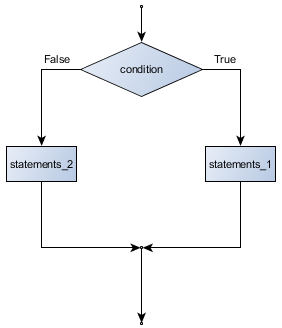
\includegraphics{flowchart_if_else.png}
\end{notice}

The syntax for an \code{if} statement looks like this:
\begin{quote}

\begin{Verbatim}[commandchars=\\\{\},numbers=left,firstnumber=1,stepnumber=1]
\PYG{k}{if} \PYG{n}{BOOLEAN} \PYG{n}{EXPRESSION}\PYG{p}{:}
    \PYG{n}{STATEMENTS\PYGZus{}1}        \PYG{c}{\PYGZsh{} Executed if condition evaluates to True}
\PYG{k}{else}\PYG{p}{:}
    \PYG{n}{STATEMENTS\PYGZus{}2}        \PYG{c}{\PYGZsh{} Executed if condition evaluates to False}
\end{Verbatim}
\end{quote}

As with the function definition from the last chapter and other compound
statements like \code{for}, the \code{if} statement consists of a header line and a body. The header
line begins with the keyword \code{if} followed by a \emph{Boolean expression} and ends with
a colon (:).

The indented statements that follow are called a \textbf{block}. The first
unindented statement marks the end of the block.

Each of the statements inside the first block of statements are executed in order if the Boolean
expression evaluates to \code{True}. The entire first block of statements
is skipped if the Boolean expression evaluates to \code{False}, and instead
all the statements indented under the \code{else} clause are executed.

There is no limit on the number of statements that can appear under the two clauses of an
\code{if} statement, but there has to be at least one statement in each block.  Occasionally, it is useful
to have a section with no statements (usually as a place keeper, or scaffolding,
for code we haven't written yet). In that case, we can use the \code{pass} statement, which
does nothing except act as a placeholder.
\begin{quote}

\begin{Verbatim}[commandchars=\\\{\},numbers=left,firstnumber=1,stepnumber=1]
\PYG{k}{if} \PYG{k}{True}\PYG{p}{:}          \PYG{c}{\PYGZsh{} This is always True,}
    \PYG{k}{pass}          \PYG{c}{\PYGZsh{}   so this is always executed, but it does nothing}
\PYG{k}{else}\PYG{p}{:}
    \PYG{k}{pass}
\end{Verbatim}
\end{quote}

\index{alternative execution}\index{branch}\index{wrapping code in a function}

\section{Omitting the \texttt{else} clause}
\label{conditionals:index-4}\label{conditionals:omitting-the-else-clause}
\begin{notice}{note}{Flowchart of an if statement with no else clause}

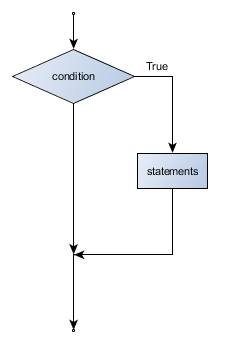
\includegraphics{flowchart_if_only.png}
\end{notice}

Another form of the \code{if} statement is one in which the \code{else} clause is omitted entirely.
In this case, when the condition evaluates to \code{True}, the statements are
executed, otherwise the flow of execution continues to the statement after the \code{if}.
\begin{quote}

\begin{Verbatim}[commandchars=\\\{\},numbers=left,firstnumber=1,stepnumber=1]
\PYG{k}{if} \PYG{n}{x} \PYG{o}{\PYGZlt{}} \PYG{l+m+mi}{0}\PYG{p}{:}
    \PYG{n+nb}{print}\PYG{p}{(}\PYG{l+s}{"}\PYG{l+s}{The negative number }\PYG{l+s}{"}\PYG{p}{,}  \PYG{n}{x}\PYG{p}{,} \PYG{l+s}{"}\PYG{l+s}{ is not valid here.}\PYG{l+s}{"}\PYG{p}{)}
    \PYG{n}{x} \PYG{o}{=} \PYG{l+m+mi}{42}
    \PYG{n+nb}{print}\PYG{p}{(}\PYG{l+s}{"}\PYG{l+s}{I}\PYG{l+s}{'}\PYG{l+s}{ve decided to use the number 42 instead.}\PYG{l+s}{"}\PYG{p}{)}

\PYG{n+nb}{print}\PYG{p}{(}\PYG{l+s}{"}\PYG{l+s}{The square root of }\PYG{l+s}{"}\PYG{p}{,} \PYG{n}{x}\PYG{p}{,} \PYG{l+s}{"}\PYG{l+s}{is}\PYG{l+s}{"}\PYG{p}{,} \PYG{n}{math}\PYG{o}{.}\PYG{n}{sqrt}\PYG{p}{(}\PYG{n}{x}\PYG{p}{)}\PYG{p}{)}
\end{Verbatim}
\end{quote}

In this case, the print function that outputs the square root is the one after the \code{if} --- not
because we left a blank line, but because of the way the code is indented.    Note too that
the function call \code{math.sqrt(x)} will give an error unless we have an \code{import math} statement,
usually placed near the top of our script.

\begin{notice}{note}{Python terminology}

Python documentation sometimes uses the term \textbf{suite} of statements to mean what we
have called a \emph{block} here. They mean the same thing, and since most other languages and
computer scientists use the word \emph{block}, we'll stick with that.

Notice too that \code{else} is not a statement.  The \code{if} statement has
two \emph{clauses}, one of which is the (optional) \code{else} clause.
\end{notice}

\index{chained conditional}\index{conditional!chained}

\section{Chained conditionals}
\label{conditionals:index-5}\label{conditionals:chained-conditionals}
Sometimes there are more than two possibilities and we need more than two
branches. One way to express a computation like that is a \textbf{chained
conditional}:
\begin{quote}

\begin{Verbatim}[commandchars=\\\{\},numbers=left,firstnumber=1,stepnumber=1]
\PYG{k}{if} \PYG{n}{x} \PYG{o}{\PYGZlt{}} \PYG{n}{y}\PYG{p}{:}
    \PYG{n}{STATEMENTS\PYGZus{}A}
\PYG{k}{elif} \PYG{n}{x} \PYG{o}{\PYGZgt{}} \PYG{n}{y}\PYG{p}{:}
    \PYG{n}{STATEMENTS\PYGZus{}B}
\PYG{k}{else}\PYG{p}{:}
    \PYG{n}{STATEMENTS\PYGZus{}C}
\end{Verbatim}
\end{quote}

\begin{notice}{note}{Flowchart of this chained conditional}

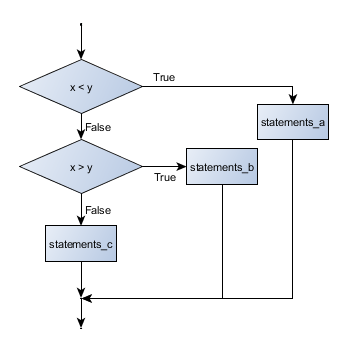
\includegraphics{flowchart_chained_conditional.png}
\end{notice}

\code{elif} is an abbreviation of \code{else if}. Again, exactly one branch will be
executed. There is no limit of the number of \code{elif} statements but only a
single (and optional) final \code{else} statement is allowed and it must be the last
branch in the statement:
\begin{quote}

\begin{Verbatim}[commandchars=\\\{\},numbers=left,firstnumber=1,stepnumber=1]
\PYG{k}{if} \PYG{n}{choice} \PYG{o}{==} \PYG{l+s}{"}\PYG{l+s}{a}\PYG{l+s}{"}\PYG{p}{:}
    \PYG{n}{function\PYGZus{}one}\PYG{p}{(}\PYG{p}{)}
\PYG{k}{elif} \PYG{n}{choice} \PYG{o}{==} \PYG{l+s}{"}\PYG{l+s}{b}\PYG{l+s}{"}\PYG{p}{:}
    \PYG{n}{function\PYGZus{}two}\PYG{p}{(}\PYG{p}{)}
\PYG{k}{elif} \PYG{n}{choice} \PYG{o}{==} \PYG{l+s}{"}\PYG{l+s}{c}\PYG{l+s}{"}\PYG{p}{:}
    \PYG{n}{function\PYGZus{}three}\PYG{p}{(}\PYG{p}{)}
\PYG{k}{else}\PYG{p}{:}
    \PYG{n+nb}{print}\PYG{p}{(}\PYG{l+s}{"}\PYG{l+s}{Invalid choice.}\PYG{l+s}{"}\PYG{p}{)}
\end{Verbatim}
\end{quote}

Each condition is checked in order. If the first is false, the next is checked,
and so on. If one of them is true, the corresponding branch executes, and the
statement ends. Even if more than one condition is true, only the first true
branch executes.

\index{nested conditionals}\index{conditionals!nested}

\section{Nested conditionals}
\label{conditionals:index-6}\label{conditionals:nested-conditionals}
One conditional can also be \textbf{nested} within another. (It is the same theme of
composibility, again!)  We could have written
the previous example as follows:

\begin{notice}{note}{Flowchart of this nested conditional}

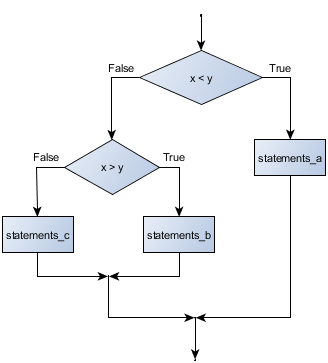
\includegraphics{flowchart_nested_conditional.png}
\end{notice}
\begin{quote}

\begin{Verbatim}[commandchars=\\\{\},numbers=left,firstnumber=1,stepnumber=1]
\PYG{k}{if} \PYG{n}{x} \PYG{o}{\PYGZlt{}} \PYG{n}{y}\PYG{p}{:}
    \PYG{n}{STATEMENTS\PYGZus{}A}
\PYG{k}{else}\PYG{p}{:}
    \PYG{k}{if} \PYG{n}{x} \PYG{o}{\PYGZgt{}} \PYG{n}{y}\PYG{p}{:}
        \PYG{n}{STATEMENTS\PYGZus{}B}
    \PYG{k}{else}\PYG{p}{:}
        \PYG{n}{STATEMENTS\PYGZus{}C}
\end{Verbatim}
\end{quote}

The outer conditional contains two branches.
The second branch contains another \code{if} statement, which
has two branches of its own. Those two branches could contain
conditional statements as well.

Although the indentation of the statements makes the structure apparent, nested
conditionals very quickly become difficult to read.  In general, it is a good
idea to avoid them when we can.

Logical operators often provide a way to simplify nested conditional
statements. For example, we can rewrite the following code using a single
conditional:
\begin{quote}

\begin{Verbatim}[commandchars=\\\{\},numbers=left,firstnumber=1,stepnumber=1]
\PYG{k}{if} \PYG{l+m+mi}{0} \PYG{o}{\PYGZlt{}} \PYG{n}{x}\PYG{p}{:}            \PYG{c}{\PYGZsh{} Assume x is an int here}
    \PYG{k}{if} \PYG{n}{x} \PYG{o}{\PYGZlt{}} \PYG{l+m+mi}{10}\PYG{p}{:}
        \PYG{n+nb}{print}\PYG{p}{(}\PYG{l+s}{"}\PYG{l+s}{x is a positive single digit.}\PYG{l+s}{"}\PYG{p}{)}
\end{Verbatim}
\end{quote}

The \code{print} function is called only if we make it past both the
conditionals, so instead of the above which uses two \code{if} statements each with
a simple condition, we could make a more complex condition using the \code{and} operator.  Now we only
need a single \code{if} statement:
\begin{quote}

\begin{Verbatim}[commandchars=\\\{\},numbers=left,firstnumber=1,stepnumber=1]
\PYG{k}{if} \PYG{l+m+mi}{0} \PYG{o}{\PYGZlt{}} \PYG{n}{x} \PYG{o+ow}{and} \PYG{n}{x} \PYG{o}{\PYGZlt{}} \PYG{l+m+mi}{10}\PYG{p}{:}
    \PYG{n+nb}{print}\PYG{p}{(}\PYG{l+s}{"}\PYG{l+s}{x is a positive single digit.}\PYG{l+s}{"}\PYG{p}{)}
\end{Verbatim}
\end{quote}

\index{return statement}\index{statement!return}

\section{The \texttt{return} statement}
\label{conditionals:index-7}\label{conditionals:the-return-statement}
The \code{return} statement, with or without a value, depending on whether the
function is fruitful or void, allows us to terminate the execution of a function
before (or when) we reach the end. One reason to use an \emph{early return} is if we detect an error
condition:
\begin{quote}

\begin{Verbatim}[commandchars=\\\{\},numbers=left,firstnumber=1,stepnumber=1]
\PYG{k}{def} \PYG{n+nf}{print\PYGZus{}square\PYGZus{}root}\PYG{p}{(}\PYG{n}{x}\PYG{p}{)}\PYG{p}{:}
    \PYG{k}{if} \PYG{n}{x} \PYG{o}{\PYGZlt{}}\PYG{o}{=} \PYG{l+m+mi}{0}\PYG{p}{:}
        \PYG{n+nb}{print}\PYG{p}{(}\PYG{l+s}{"}\PYG{l+s}{Positive numbers only, please.}\PYG{l+s}{"}\PYG{p}{)}
        \PYG{k}{return}

    \PYG{n}{result} \PYG{o}{=} \PYG{n}{x}\PYG{o}{*}\PYG{o}{*}\PYG{l+m+mf}{0.5}
    \PYG{n+nb}{print}\PYG{p}{(}\PYG{l+s}{"}\PYG{l+s}{The square root of}\PYG{l+s}{"}\PYG{p}{,} \PYG{n}{x}\PYG{p}{,} \PYG{l+s}{"}\PYG{l+s}{is}\PYG{l+s}{"}\PYG{p}{,} \PYG{n}{result}\PYG{p}{)}
\end{Verbatim}
\end{quote}

The function \code{print\_square\_root} has a parameter named \code{x}. The first thing
it does is check whether \code{x} is less than or equal to 0, in which case it
displays an error message and then uses \code{return} to exit the function. The
flow of execution immediately returns to the caller, and the remaining lines of
the function are not executed.


\section{Logical opposites}
\label{conditionals:logical-opposites}
Each of the six relational operators has a logical opposite: for example,
suppose we can get a driving licence when our age is greater or equal to 17,
we can \emph{not} get the driving licence when we are less than 17.

Notice that the opposite of \code{\textgreater{}=} is \code{\textless{}}.
\begin{quote}

\begin{tabulary}{\linewidth}{|L|L|}
\hline
\textbf{
operator
} & \textbf{
logical opposite
}\\\hline

==
 & 
!=
\\\hline

!=
 & 
==
\\\hline

\textless{}
 & 
\textgreater{}=
\\\hline

\textless{}=
 & 
\textgreater{}
\\\hline

\textgreater{}
 & 
\textless{}=
\\\hline

\textgreater{}=
 & 
\textless{}
\\\hline
\end{tabulary}

\end{quote}

Understanding these logical opposites allows us to sometimes get rid of \code{not}
operators.  \code{not} operators are often quite difficult to read in computer code, and
our intentions will usually be clearer if we can eliminate them.

For example, if we wrote this Python:
\begin{quote}

\begin{Verbatim}[commandchars=\\\{\},numbers=left,firstnumber=1,stepnumber=1]
\PYG{k}{if} \PYG{o+ow}{not} \PYG{p}{(}\PYG{n}{age} \PYG{o}{\PYGZgt{}}\PYG{o}{=} \PYG{l+m+mi}{17}\PYG{p}{)}\PYG{p}{:}
    \PYG{n+nb}{print}\PYG{p}{(}\PYG{l+s}{"}\PYG{l+s}{Hey, you}\PYG{l+s}{'}\PYG{l+s}{re too young to get a driving licence!}\PYG{l+s}{"}\PYG{p}{)}
\end{Verbatim}
\end{quote}

it would probably be clearer to use the simplification laws, and to
write instead:
\begin{quote}

\begin{Verbatim}[commandchars=\\\{\},numbers=left,firstnumber=1,stepnumber=1]
\PYG{k}{if} \PYG{n}{age} \PYG{o}{\PYGZlt{}} \PYG{l+m+mi}{17}\PYG{p}{:}
    \PYG{n+nb}{print}\PYG{p}{(}\PYG{l+s}{"}\PYG{l+s}{Hey, you}\PYG{l+s}{'}\PYG{l+s}{re too young to get a driving licence!}\PYG{l+s}{"}\PYG{p}{)}
\end{Verbatim}
\end{quote}

Two powerful simplification laws (called de Morgan's laws) that are often
helpful when dealing with complicated Boolean expressions are:
\begin{quote}

\begin{Verbatim}[commandchars=\\\{\}]
\PYG{g+go}{not (x and y)  ==  (not x) or (not y)}
\PYG{g+go}{not (x or y)   ==  (not x) and (not y)}
\end{Verbatim}
\end{quote}

For example, suppose we can slay the dragon only if our magic
lightsabre sword is charged to 90\% or higher,
and we have 100 or more energy units in our protective shield.
We find this fragment of Python code in the game:
\begin{quote}

\begin{Verbatim}[commandchars=\\\{\},numbers=left,firstnumber=1,stepnumber=1]
\PYG{k}{if} \PYG{o+ow}{not} \PYG{p}{(}\PYG{p}{(}\PYG{n}{sword\PYGZus{}charge} \PYG{o}{\PYGZgt{}}\PYG{o}{=} \PYG{l+m+mf}{0.90}\PYG{p}{)} \PYG{o+ow}{and} \PYG{p}{(}\PYG{n}{shield\PYGZus{}energy} \PYG{o}{\PYGZgt{}}\PYG{o}{=} \PYG{l+m+mi}{100}\PYG{p}{)}\PYG{p}{)}\PYG{p}{:}
    \PYG{n+nb}{print}\PYG{p}{(}\PYG{l+s}{"}\PYG{l+s}{Your attack has no effect, the dragon fries you to a crisp!}\PYG{l+s}{"}\PYG{p}{)}
\PYG{k}{else}\PYG{p}{:}
    \PYG{n+nb}{print}\PYG{p}{(}\PYG{l+s}{"}\PYG{l+s}{The dragon crumples in a heap. You rescue the gorgeous princess!}\PYG{l+s}{"}\PYG{p}{)}
\end{Verbatim}
\end{quote}

de Morgan's laws together with the logical opposites would let us
rework the condition in a (perhaps) easier to understand way like this:
\begin{quote}

\begin{Verbatim}[commandchars=\\\{\},numbers=left,firstnumber=1,stepnumber=1]
\PYG{k}{if} \PYG{p}{(}\PYG{n}{sword\PYGZus{}charge} \PYG{o}{\PYGZlt{}} \PYG{l+m+mf}{0.90}\PYG{p}{)} \PYG{o+ow}{or} \PYG{p}{(}\PYG{n}{shield\PYGZus{}energy} \PYG{o}{\PYGZlt{}} \PYG{l+m+mi}{100}\PYG{p}{)}\PYG{p}{:}
    \PYG{n+nb}{print}\PYG{p}{(}\PYG{l+s}{"}\PYG{l+s}{Your attack has no effect, the dragon fries you to a crisp!}\PYG{l+s}{"}\PYG{p}{)}
\PYG{k}{else}\PYG{p}{:}
    \PYG{n+nb}{print}\PYG{p}{(}\PYG{l+s}{"}\PYG{l+s}{The dragon crumples in a heap. You rescue the gorgeous princess!}\PYG{l+s}{"}\PYG{p}{)}
\end{Verbatim}
\end{quote}

We could also get rid of the \code{not} by swapping around the \code{then} and
\code{else} parts of the conditional.  So here is a third version, also equivalent:
\begin{quote}

\begin{Verbatim}[commandchars=\\\{\},numbers=left,firstnumber=1,stepnumber=1]
\PYG{k}{if} \PYG{p}{(}\PYG{n}{sword\PYGZus{}charge} \PYG{o}{\PYGZgt{}}\PYG{o}{=} \PYG{l+m+mf}{0.90}\PYG{p}{)} \PYG{o+ow}{and} \PYG{p}{(}\PYG{n}{shield\PYGZus{}energy} \PYG{o}{\PYGZgt{}}\PYG{o}{=} \PYG{l+m+mi}{100}\PYG{p}{)}\PYG{p}{:}
    \PYG{n+nb}{print}\PYG{p}{(}\PYG{l+s}{"}\PYG{l+s}{The dragon crumples in a heap. You rescue the gorgeous princess!}\PYG{l+s}{"}\PYG{p}{)}
\PYG{k}{else}\PYG{p}{:}
    \PYG{n+nb}{print}\PYG{p}{(}\PYG{l+s}{"}\PYG{l+s}{Your attack has no effect, the dragon fries you to a crisp!}\PYG{l+s}{"}\PYG{p}{)}
\end{Verbatim}
\end{quote}

This version is probably the best of the three, because it very closely matches
the initial English statement. Clarity of our code (for other humans),
and making it easy to see that the code does what was expected should always
be a high priority.

As our programming skills develop we'll find we have
more than one way to solve any problem.  So good programs are \emph{designed}.
We make choices that favour clarity, simplicity, and elegance.  The job
title \emph{software architect} says a lot about what we do --- we are \emph{architects}
who engineer our products to balance beauty, functionality, simplicity and
clarity in our creations.

\begin{notice}{tip}{Tip:}
Once our program works, we should play around a bit trying to polish it up.
Write good comments.  Think about whether the code would be clearer with
different variable names.  Could we have done it more elegantly?  Should
we rather use a function?  Can we simplify the conditionals?

We think of our code as our creation, our work of art!  We make it great.
\end{notice}

\index{type conversion}\index{type!conversion}

\section{Type conversion}
\label{conditionals:type-conversion}\label{conditionals:index-8}
We've had a first look at this in an earlier chapter.  Seeing it again won't hurt!

Many Python types come with a built-in function that attempts to convert values
of another type into its own type. The \code{int} function, for example,
takes any value and converts it to an integer, if possible, or complains
otherwise:
\begin{quote}

\begin{Verbatim}[commandchars=\\\{\}]
\PYG{g+gp}{\PYGZgt{}\PYGZgt{}\PYGZgt{} }\PYG{n+nb}{int}\PYG{p}{(}\PYG{l+s}{"}\PYG{l+s}{32}\PYG{l+s}{"}\PYG{p}{)}
\PYG{g+go}{32}
\PYG{g+gp}{\PYGZgt{}\PYGZgt{}\PYGZgt{} }\PYG{n+nb}{int}\PYG{p}{(}\PYG{l+s}{"}\PYG{l+s}{Hello}\PYG{l+s}{"}\PYG{p}{)}
\PYG{g+go}{ValueError: invalid literal for int() with base 10: 'Hello'}
\end{Verbatim}
\end{quote}

\code{int} can also convert floating-point values to integers, but remember
that it truncates the fractional part:
\begin{quote}

\begin{Verbatim}[commandchars=\\\{\}]
\PYG{g+gp}{\PYGZgt{}\PYGZgt{}\PYGZgt{} }\PYG{n+nb}{int}\PYG{p}{(}\PYG{o}{-}\PYG{l+m+mf}{2.3}\PYG{p}{)}
\PYG{g+go}{-2}
\PYG{g+gp}{\PYGZgt{}\PYGZgt{}\PYGZgt{} }\PYG{n+nb}{int}\PYG{p}{(}\PYG{l+m+mf}{3.99999}\PYG{p}{)}
\PYG{g+go}{3}
\PYG{g+gp}{\PYGZgt{}\PYGZgt{}\PYGZgt{} }\PYG{n+nb}{int}\PYG{p}{(}\PYG{l+s}{"}\PYG{l+s}{42}\PYG{l+s}{"}\PYG{p}{)}
\PYG{g+go}{42}
\PYG{g+gp}{\PYGZgt{}\PYGZgt{}\PYGZgt{} }\PYG{n+nb}{int}\PYG{p}{(}\PYG{l+m+mf}{1.0}\PYG{p}{)}
\PYG{g+go}{1}
\end{Verbatim}
\end{quote}

The \code{float} function converts integers and strings to floating-point
numbers:
\begin{quote}

\begin{Verbatim}[commandchars=\\\{\}]
\PYG{g+gp}{\PYGZgt{}\PYGZgt{}\PYGZgt{} }\PYG{n+nb}{float}\PYG{p}{(}\PYG{l+m+mi}{32}\PYG{p}{)}
\PYG{g+go}{32.0}
\PYG{g+gp}{\PYGZgt{}\PYGZgt{}\PYGZgt{} }\PYG{n+nb}{float}\PYG{p}{(}\PYG{l+s}{"}\PYG{l+s}{3.14159}\PYG{l+s}{"}\PYG{p}{)}
\PYG{g+go}{3.14159}
\PYG{g+gp}{\PYGZgt{}\PYGZgt{}\PYGZgt{} }\PYG{n+nb}{float}\PYG{p}{(}\PYG{l+m+mi}{1}\PYG{p}{)}
\PYG{g+go}{1.0}
\end{Verbatim}
\end{quote}

It may seem odd that Python distinguishes the integer value \code{1} from the
floating-point value \code{1.0}. They may represent the same number, but they
belong to different types. The reason is that they are represented differently
inside the computer.

The \code{str} function converts any argument given to it to type
\code{string}:
\begin{quote}

\begin{Verbatim}[commandchars=\\\{\}]
\PYG{g+gp}{\PYGZgt{}\PYGZgt{}\PYGZgt{} }\PYG{n+nb}{str}\PYG{p}{(}\PYG{l+m+mi}{32}\PYG{p}{)}
\PYG{g+go}{'32'}
\PYG{g+gp}{\PYGZgt{}\PYGZgt{}\PYGZgt{} }\PYG{n+nb}{str}\PYG{p}{(}\PYG{l+m+mf}{3.14149}\PYG{p}{)}
\PYG{g+go}{'3.14149'}
\PYG{g+gp}{\PYGZgt{}\PYGZgt{}\PYGZgt{} }\PYG{n+nb}{str}\PYG{p}{(}\PYG{k}{True}\PYG{p}{)}
\PYG{g+go}{'True'}
\PYG{g+gp}{\PYGZgt{}\PYGZgt{}\PYGZgt{} }\PYG{n+nb}{str}\PYG{p}{(}\PYG{n}{true}\PYG{p}{)}
\PYG{g+gt}{Traceback (most recent call last):}
  File \PYG{n+nb}{"\PYGZlt{}interactive input\PYGZgt{}"}, line \PYG{l+m}{1}, in \PYG{n}{\PYGZlt{}module\PYGZgt{}}
\PYG{g+gr}{NameError}: \PYG{n}{name 'true' is not defined}
\end{Verbatim}
\end{quote}

\code{str} will work with any value and convert it into a string.  As
mentioned earlier, \code{True} is Boolean value; \code{true} is just an ordinary variable name,
and is not defined here, so we get an error.

\index{bar chart}

\section{A Turtle Bar Chart}
\label{conditionals:a-turtle-bar-chart}\label{conditionals:index-9}
The turtle has a lot more power than we've seen so far. The full
documentation can be found at
\href{http://docs.python.org/py3k/library/turtle.html}{http://docs.python.org/py3k/library/turtle.html}
or within PyScripter, use \emph{Help} and search for the turtle module.

Here are a couple of new tricks for our turtles:
\begin{itemize}
\item {} 
We can get a turtle to display text on the canvas at the turtle's current position.  The method to do that is
\code{alex.write("Hello")}.

\item {} 
We can fill a shape (circle, semicircle, triangle, etc.) with a color.  It is a two-step process.
First we call the method \code{alex.begin\_fill()}, then we draw the shape, then we call \code{alex.end\_fill()}.

\item {} 
We've previously set the color of our turtle --- we can now also set its fill color, which need not
be the same as the turtle and the pen color.  We use \code{alex.color("blue","red")} to set the turtle
to draw in blue, and fill in red.

\end{itemize}

Ok, so can we get tess to draw a bar chart?  Let us start with some data to be charted,

\code{xs = {[}48, 117, 200, 240, 160, 260, 220{]}}

Corresponding to each data measurement, we'll draw a simple rectangle of that height, with a fixed width.
\begin{quote}

\begin{Verbatim}[commandchars=\\\{\},numbers=left,firstnumber=1,stepnumber=1]
\PYG{k}{def} \PYG{n+nf}{draw\PYGZus{}bar}\PYG{p}{(}\PYG{n}{t}\PYG{p}{,} \PYG{n}{height}\PYG{p}{)}\PYG{p}{:}
    \PYG{l+s+sd}{""" Get turtle t to draw one bar, of height. """}
    \PYG{n}{t}\PYG{o}{.}\PYG{n}{left}\PYG{p}{(}\PYG{l+m+mi}{90}\PYG{p}{)}
    \PYG{n}{t}\PYG{o}{.}\PYG{n}{forward}\PYG{p}{(}\PYG{n}{height}\PYG{p}{)}     \PYG{c}{\PYGZsh{} Draw up the left side}
    \PYG{n}{t}\PYG{o}{.}\PYG{n}{right}\PYG{p}{(}\PYG{l+m+mi}{90}\PYG{p}{)}
    \PYG{n}{t}\PYG{o}{.}\PYG{n}{forward}\PYG{p}{(}\PYG{l+m+mi}{40}\PYG{p}{)}         \PYG{c}{\PYGZsh{} Width of bar, along the top}
    \PYG{n}{t}\PYG{o}{.}\PYG{n}{right}\PYG{p}{(}\PYG{l+m+mi}{90}\PYG{p}{)}
    \PYG{n}{t}\PYG{o}{.}\PYG{n}{forward}\PYG{p}{(}\PYG{n}{height}\PYG{p}{)}     \PYG{c}{\PYGZsh{} And down again!}
    \PYG{n}{t}\PYG{o}{.}\PYG{n}{left}\PYG{p}{(}\PYG{l+m+mi}{90}\PYG{p}{)}            \PYG{c}{\PYGZsh{} Put the turtle facing the way we found it.}
    \PYG{n}{t}\PYG{o}{.}\PYG{n}{forward}\PYG{p}{(}\PYG{l+m+mi}{10}\PYG{p}{)}         \PYG{c}{\PYGZsh{} Leave small gap after each bar}

\PYG{o}{.}\PYG{o}{.}\PYG{o}{.}
\PYG{k}{for} \PYG{n}{v} \PYG{o+ow}{in} \PYG{n}{xs}\PYG{p}{:}              \PYG{c}{\PYGZsh{} Assume xs and tess are ready}
    \PYG{n}{draw\PYGZus{}bar}\PYG{p}{(}\PYG{n}{tess}\PYG{p}{,} \PYG{n}{v}\PYG{p}{)}
\end{Verbatim}
\end{quote}
\begin{quote}

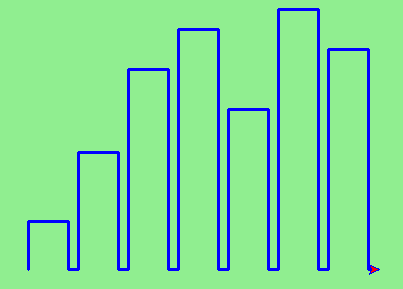
\includegraphics{tess_bar_1.png}
\end{quote}

Ok, not fantasically impressive, but it is a nice start!  The important thing here
was the mental chunking, or how we broke the problem into smaller pieces. Our chunk
is to draw one bar, and we wrote a function to do that. Then, for the whole
chart, we repeatedly called our function.

Next, at the top of each bar, we'll print the value of the data.
We'll do this in the body of \code{draw\_bar}, by adding   \code{t.write('  ' + str(height))}
as the new third line of the body.
We've put a little space in front of the number, and turned the
number into a string.  Without this extra space we tend
to cramp our text awkwardly against the bar to the left.
The result looks a lot better now:
\begin{quote}

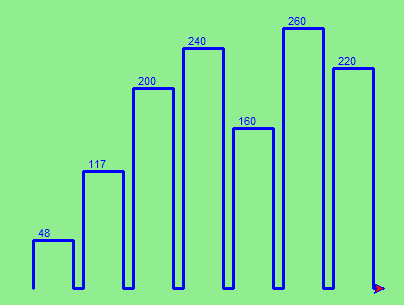
\includegraphics{tess_bar_2.png}
\end{quote}

And now we'll add two lines to fill each bar.  Our final program now looks like this:
\begin{quote}

\begin{Verbatim}[commandchars=\\\{\},numbers=left,firstnumber=1,stepnumber=1]
\PYG{k}{def} \PYG{n+nf}{draw\PYGZus{}bar}\PYG{p}{(}\PYG{n}{t}\PYG{p}{,} \PYG{n}{height}\PYG{p}{)}\PYG{p}{:}
    \PYG{l+s+sd}{""" Get turtle t to draw one bar, of height. """}
    \PYG{n}{t}\PYG{o}{.}\PYG{n}{begin\PYGZus{}fill}\PYG{p}{(}\PYG{p}{)}           \PYG{c}{\PYGZsh{} Added this line}
    \PYG{n}{t}\PYG{o}{.}\PYG{n}{left}\PYG{p}{(}\PYG{l+m+mi}{90}\PYG{p}{)}
    \PYG{n}{t}\PYG{o}{.}\PYG{n}{forward}\PYG{p}{(}\PYG{n}{height}\PYG{p}{)}
    \PYG{n}{t}\PYG{o}{.}\PYG{n}{write}\PYG{p}{(}\PYG{l+s}{"}\PYG{l+s}{  }\PYG{l+s}{"}\PYG{o}{+} \PYG{n+nb}{str}\PYG{p}{(}\PYG{n}{height}\PYG{p}{)}\PYG{p}{)}
    \PYG{n}{t}\PYG{o}{.}\PYG{n}{right}\PYG{p}{(}\PYG{l+m+mi}{90}\PYG{p}{)}
    \PYG{n}{t}\PYG{o}{.}\PYG{n}{forward}\PYG{p}{(}\PYG{l+m+mi}{40}\PYG{p}{)}
    \PYG{n}{t}\PYG{o}{.}\PYG{n}{right}\PYG{p}{(}\PYG{l+m+mi}{90}\PYG{p}{)}
    \PYG{n}{t}\PYG{o}{.}\PYG{n}{forward}\PYG{p}{(}\PYG{n}{height}\PYG{p}{)}
    \PYG{n}{t}\PYG{o}{.}\PYG{n}{left}\PYG{p}{(}\PYG{l+m+mi}{90}\PYG{p}{)}
    \PYG{n}{t}\PYG{o}{.}\PYG{n}{end\PYGZus{}fill}\PYG{p}{(}\PYG{p}{)}             \PYG{c}{\PYGZsh{} Added this line}
    \PYG{n}{t}\PYG{o}{.}\PYG{n}{forward}\PYG{p}{(}\PYG{l+m+mi}{10}\PYG{p}{)}

\PYG{n}{wn} \PYG{o}{=} \PYG{n}{turtle}\PYG{o}{.}\PYG{n}{Screen}\PYG{p}{(}\PYG{p}{)}         \PYG{c}{\PYGZsh{} Set up the window and its attributes}
\PYG{n}{wn}\PYG{o}{.}\PYG{n}{bgcolor}\PYG{p}{(}\PYG{l+s}{"}\PYG{l+s}{lightgreen}\PYG{l+s}{"}\PYG{p}{)}

\PYG{n}{tess} \PYG{o}{=} \PYG{n}{turtle}\PYG{o}{.}\PYG{n}{Turtle}\PYG{p}{(}\PYG{p}{)}       \PYG{c}{\PYGZsh{} Create tess and set some attributes}
\PYG{n}{tess}\PYG{o}{.}\PYG{n}{color}\PYG{p}{(}\PYG{l+s}{"}\PYG{l+s}{blue}\PYG{l+s}{"}\PYG{p}{,} \PYG{l+s}{"}\PYG{l+s}{red}\PYG{l+s}{"}\PYG{p}{)}
\PYG{n}{tess}\PYG{o}{.}\PYG{n}{pensize}\PYG{p}{(}\PYG{l+m+mi}{3}\PYG{p}{)}

\PYG{n}{xs} \PYG{o}{=} \PYG{p}{[}\PYG{l+m+mi}{48}\PYG{p}{,}\PYG{l+m+mi}{117}\PYG{p}{,}\PYG{l+m+mi}{200}\PYG{p}{,}\PYG{l+m+mi}{240}\PYG{p}{,}\PYG{l+m+mi}{160}\PYG{p}{,}\PYG{l+m+mi}{260}\PYG{p}{,}\PYG{l+m+mi}{220}\PYG{p}{]}

\PYG{k}{for} \PYG{n}{a} \PYG{o+ow}{in} \PYG{n}{xs}\PYG{p}{:}
    \PYG{n}{draw\PYGZus{}bar}\PYG{p}{(}\PYG{n}{tess}\PYG{p}{,} \PYG{n}{a}\PYG{p}{)}

\PYG{n}{wn}\PYG{o}{.}\PYG{n}{mainloop}\PYG{p}{(}\PYG{p}{)}
\end{Verbatim}
\end{quote}

It produces the following, which is more satisfying:
\begin{quote}

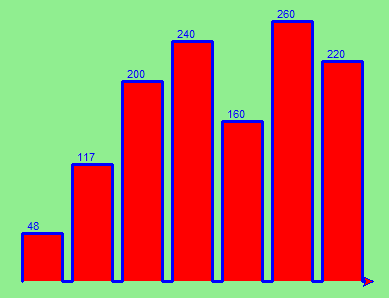
\includegraphics{tess_bar_3.png}
\end{quote}

Mmm.  Perhaps the bars should not be joined to each other at the bottom.  We'll need to pick up the pen while making the gap between the bars.  We'll leave that as an exercise for you!


\section{Glossary}
\label{conditionals:glossary}\begin{description}
\item[{\index{block|textbf}block}] \leavevmode\phantomsection\label{conditionals:term-block}
A group of consecutive statements with the same indentation.

\item[{\index{body|textbf}body}] \leavevmode\phantomsection\label{conditionals:term-body}
The block of statements in a compound statement that follows the
header.

\item[{\index{Boolean algebra|textbf}Boolean algebra}] \leavevmode\phantomsection\label{conditionals:term-boolean-algebra}
Some rules for rearranging and reasoning about Boolean expressions.

\item[{\index{Boolean expression|textbf}Boolean expression}] \leavevmode\phantomsection\label{conditionals:term-boolean-expression}
An expression that is either true or false.

\item[{\index{Boolean value|textbf}Boolean value}] \leavevmode\phantomsection\label{conditionals:term-boolean-value}
There are exactly two Boolean values: \code{True} and \code{False}. Boolean
values result when a Boolean expression is evaluated by the Python
interepreter.  They have type \code{bool}.

\item[{\index{branch|textbf}branch}] \leavevmode\phantomsection\label{conditionals:term-branch}
One of the possible paths of the flow of execution determined by
conditional execution.

\item[{\index{chained conditional|textbf}chained conditional}] \leavevmode\phantomsection\label{conditionals:term-chained-conditional}
A conditional branch with more than two possible flows of execution. In
Python chained conditionals are written with \code{if ... elif ... else}
statements.

\item[{\index{comparison operator|textbf}comparison operator}] \leavevmode\phantomsection\label{conditionals:term-comparison-operator}
One of the six operators that compares two values: \code{==}, \code{!=}, \code{\textgreater{}},
\code{\textless{}}, \code{\textgreater{}=}, and \code{\textless{}=}.

\item[{\index{condition|textbf}condition}] \leavevmode\phantomsection\label{conditionals:term-condition}
The Boolean expression in a conditional statement that determines which
branch is executed.

\item[{\index{conditional statement|textbf}conditional statement}] \leavevmode\phantomsection\label{conditionals:term-conditional-statement}
A statement that controls the flow of execution depending on some
condition. In Python the keywords \code{if}, \code{elif}, and \code{else} are
used for conditional statements.

\item[{\index{logical operator|textbf}logical operator}] \leavevmode\phantomsection\label{conditionals:term-logical-operator}
One of the operators that combines Boolean expressions: \code{and},
\code{or}, and \code{not}.

\item[{\index{nesting|textbf}nesting}] \leavevmode\phantomsection\label{conditionals:term-nesting}
One program structure within another, such as a conditional statement
inside a branch of another conditional statement.

\item[{\index{prompt|textbf}prompt}] \leavevmode\phantomsection\label{conditionals:term-prompt}
A visual cue that tells the user that the system is ready to accept input data.

\item[{\index{truth table|textbf}truth table}] \leavevmode\phantomsection\label{conditionals:term-truth-table}
A concise table of Boolean values that can describe the semantics
of an operator.

\item[{\index{type conversion|textbf}type conversion}] \leavevmode\phantomsection\label{conditionals:term-type-conversion}
An explicit function call that takes a value of one type and computes a
corresponding value of another type.

\item[{\index{wrapping code in a function|textbf}wrapping code in a function}] \leavevmode\phantomsection\label{conditionals:term-wrapping-code-in-a-function}
The process of adding a function header and parameters to a sequence
of program statements is often refered to as ``wrapping the code in
a function''.  This process is very useful whenever the program
statements in question are going to be used multiple times.  It is
even more useful when it allows the programmer to express their mental
chunking, and how they've broken a complex problem into pieces.

\end{description}


\section{Exercises}
\label{conditionals:exercises}\begin{enumerate}
\item {} 
Assume the days of the week are numbered 0,1,2,3,4,5,6 from Sunday to Saturday.
Write a function which is given the day number, and it returns the day name (a string).

\item {} 
You go on a wonderful holiday (perhaps to jail, if you don't like happy exercises)
leaving on day number 3 (a Wednesday).  You return home after 137 sleeps.
Write a general version of the program which asks for the starting day number, and
the length of your stay, and it will tell you the name of day of the week you will return on.

\item {} 
Give the logical opposites of these conditions
\begin{enumerate}
\item {} 
\code{a \textgreater{} b}

\item {} 
\code{a \textgreater{}= b}

\item {} 
\code{a \textgreater{}= 18  and  day == 3}

\item {} 
\code{a \textgreater{}= 18  and  day != 3}

\end{enumerate}

\item {} 
What do these expressions evaluate to?
\begin{enumerate}
\item {} 
\code{3 == 3}

\item {} 
\code{3 != 3}

\item {} 
\code{3 \textgreater{}= 4}

\item {} 
\code{not (3 \textless{} 4)}

\end{enumerate}

\item {} 
Complete this truth table:
\begin{quote}

\begin{tabulary}{\linewidth}{|L|L|L|L|}
\hline
\textbf{
p
} & \textbf{
q
} & \textbf{
r
} & \textbf{
(not (p and q)) or r
}\\\hline

F
 & 
F
 & 
F
 & 
?
\\\hline

F
 & 
F
 & 
T
 & 
?
\\\hline

F
 & 
T
 & 
F
 & 
?
\\\hline

F
 & 
T
 & 
T
 & 
?
\\\hline

T
 & 
F
 & 
F
 & 
?
\\\hline

T
 & 
F
 & 
T
 & 
?
\\\hline

T
 & 
T
 & 
F
 & 
?
\\\hline

T
 & 
T
 & 
T
 & 
?
\\\hline
\end{tabulary}

\end{quote}

\item {} 
Write a function which is given an exam mark, and it returns a string ---
the grade for that mark --- according to this scheme:
\begin{quote}

\begin{tabulary}{\linewidth}{|L|L|}
\hline
\textbf{
Mark
} & \textbf{
Grade
}\\\hline

\textgreater{}= 75
 & 
First
\\\hline

{[}70-75)
 & 
Upper Second
\\\hline

{[}60-70)
 & 
Second
\\\hline

{[}50-60)
 & 
Third
\\\hline

{[}45-50)
 & 
F1 Supp
\\\hline

{[}40-45)
 & 
F2
\\\hline

\textless{} 40
 & 
F3
\\\hline
\end{tabulary}

\end{quote}

The square and round brackets denote closed and open intervals.
A closed interval includes the number, and open interval excludes it.   So 39.99999 gets grade F3, but 40 gets grade F2.
Assume

\begin{Verbatim}[commandchars=\\\{\}]
\PYG{n}{xs} \PYG{o}{=} \PYG{p}{[}\PYG{l+m+mi}{83}\PYG{p}{,} \PYG{l+m+mi}{75}\PYG{p}{,} \PYG{l+m+mf}{74.9}\PYG{p}{,} \PYG{l+m+mi}{70}\PYG{p}{,} \PYG{l+m+mf}{69.9}\PYG{p}{,} \PYG{l+m+mi}{65}\PYG{p}{,} \PYG{l+m+mi}{60}\PYG{p}{,} \PYG{l+m+mf}{59.9}\PYG{p}{,} \PYG{l+m+mi}{55}\PYG{p}{,} \PYG{l+m+mi}{50}\PYG{p}{,}
                     \PYG{l+m+mf}{49.9}\PYG{p}{,} \PYG{l+m+mi}{45}\PYG{p}{,} \PYG{l+m+mf}{44.9}\PYG{p}{,} \PYG{l+m+mi}{40}\PYG{p}{,} \PYG{l+m+mf}{39.9}\PYG{p}{,} \PYG{l+m+mi}{2}\PYG{p}{,} \PYG{l+m+mi}{0}\PYG{p}{]}
\end{Verbatim}

Test your function by printing the mark and the grade for all the elements in this list.

\item {} 
Modify the turtle bar chart program so that the pen is up for the small gaps between each bar.

\item {} 
Modify the turtle bar chart program so that the bar for any value
of 200 or more is filled with red, values between {[}100 and 200) are filled with yellow,
and bars representing values less than 100 are filled with green.

\item {} 
In the turtle bar chart program, what do you expect to happen if one or more
of the data values in the list is negative?   Try it out.  Change the
program so that when it prints the text value for the negative bars, it puts
the text below the bottom of the bar.

\item {} 
Write a function \code{find\_hypot} which, given the length of two sides of a right-angled triangle, returns
the length of the hypotenuse.  (Hint:  \code{x ** 0.5} will return the square root.)

\item {} 
Write a function \code{is\_rightangled} which, given the length of three sides of a triangle,
will determine whether the triangle is right-angled.  Assume that the third argument to the
function is always the longest side.  It will return \code{True} if the triangle
is right-angled, or \code{False} otherwise.

Hint: Floating point arithmetic is not always exactly accurate,
so it is not safe to test floating point numbers for equality.
If a good programmer wants to know whether
\code{x} is equal or close enough to \code{y}, they would probably code it up as:

\begin{Verbatim}[commandchars=\\\{\}]
\PYG{k}{if}  \PYG{n+nb}{abs}\PYG{p}{(}\PYG{n}{x}\PYG{o}{-}\PYG{n}{y}\PYG{p}{)} \PYG{o}{\PYGZlt{}} \PYG{l+m+mf}{0.000001}\PYG{p}{:}    \PYG{c}{\PYGZsh{} If x is approximately equal to y}
    \PYG{o}{.}\PYG{o}{.}\PYG{o}{.}
\end{Verbatim}

\item {} 
Extend the above program so that the sides can be given to the function in any order.

\item {} 
If you're intrigued by why floating point arithmetic is sometimes inaccurate, on a piece
of paper, divide 10 by 3 and write down the decimal result.  You'll find it does not terminate,
so you'll need an infinitely long sheet of paper.  The \emph{representation} of numbers in computer
memory has similar problems: memory is finite, and some digits may have to be discarded. So small
inaccuracies creep in.   Try this script:

\end{enumerate}
\begin{quote}

\begin{Verbatim}[commandchars=\\\{\}]
\PYG{g+gp}{\PYGZgt{}\PYGZgt{}\PYGZgt{} }\PYG{k+kn}{import} \PYG{n+nn}{math}
\PYG{g+gp}{\PYGZgt{}\PYGZgt{}\PYGZgt{} }\PYG{n}{a} \PYG{o}{=} \PYG{n}{math}\PYG{o}{.}\PYG{n}{sqrt}\PYG{p}{(}\PYG{l+m+mi}{2}\PYG{p}{)}
\PYG{g+gp}{\PYGZgt{}\PYGZgt{}\PYGZgt{} }\PYG{n}{a}
\PYG{g+gp}{\PYGZgt{}\PYGZgt{}\PYGZgt{} }\PYG{n}{a}\PYG{o}{*}\PYG{n}{a} \PYG{o}{==} \PYG{l+m+mi}{2}
\end{Verbatim}
\end{quote}

\begin{DUlineblock}{0em}
\item[] 
\end{DUlineblock}


\chapter{Fruitful functions}
\label{fruitful_functions:fruitful-functions}\label{fruitful_functions::doc}
\index{return statement}\index{return value}\index{temporary variable}\index{dead code}\index{None}\index{unreachable code}
\index{value}\index{variable!temporary}

\section{Return values}
\label{fruitful_functions:return-values}\label{fruitful_functions:index-1}
The built-in functions we have used, such as \code{abs}, \code{pow}, \code{int}, \code{max}, and \code{range},
have produced results. Calling each of these functions generates a value, which
we usually assign to a variable or use as part of an expression.
\begin{quote}

\begin{Verbatim}[commandchars=\\\{\},numbers=left,firstnumber=1,stepnumber=1]
\PYG{n}{biggest} \PYG{o}{=} \PYG{n+nb}{max}\PYG{p}{(}\PYG{l+m+mi}{3}\PYG{p}{,} \PYG{l+m+mi}{7}\PYG{p}{,} \PYG{l+m+mi}{2}\PYG{p}{,} \PYG{l+m+mi}{5}\PYG{p}{)}
\PYG{n}{x} \PYG{o}{=} \PYG{n+nb}{abs}\PYG{p}{(}\PYG{l+m+mi}{3} \PYG{o}{-} \PYG{l+m+mi}{11}\PYG{p}{)} \PYG{o}{+} \PYG{l+m+mi}{10}
\end{Verbatim}
\end{quote}

We also wrote our own function to return the final amount for a compound interest calculation.

In this chapter, we are going to write more functions that return values, which we
will call \emph{fruitful functions}, for want of a better name.  The first example
is \code{area}, which returns the area of a circle with the given radius:
\begin{quote}

\begin{Verbatim}[commandchars=\\\{\},numbers=left,firstnumber=1,stepnumber=1]
\PYG{k}{def} \PYG{n+nf}{area}\PYG{p}{(}\PYG{n}{radius}\PYG{p}{)}\PYG{p}{:}
    \PYG{n}{b} \PYG{o}{=} \PYG{l+m+mf}{3.14159} \PYG{o}{*} \PYG{n}{radius}\PYG{o}{*}\PYG{o}{*}\PYG{l+m+mi}{2}
    \PYG{k}{return} \PYG{n}{b}
\end{Verbatim}
\end{quote}

We have seen the \code{return} statement before, but in a fruitful function the
\code{return} statement includes a \textbf{return value}. This statement means: evaluate
the return expression, and then return it immediately as the result (the fruit)
of this function.  The expression provided can be arbitrarily complicated,
so we could have written this function like this:
\begin{quote}

\begin{Verbatim}[commandchars=\\\{\},numbers=left,firstnumber=1,stepnumber=1]
\PYG{k}{def} \PYG{n+nf}{area}\PYG{p}{(}\PYG{n}{radius}\PYG{p}{)}\PYG{p}{:}
    \PYG{k}{return} \PYG{l+m+mf}{3.14159} \PYG{o}{*} \PYG{n}{radius} \PYG{o}{*} \PYG{n}{radius}
\end{Verbatim}
\end{quote}

On the other hand, \textbf{temporary variables} like \code{b} above often make debugging
easier.

Sometimes it is useful to have multiple return statements, one in each branch
of a conditional. We have already seen the built-in \code{abs}, now we see how to
write our own:
\begin{quote}

\begin{Verbatim}[commandchars=\\\{\},numbers=left,firstnumber=1,stepnumber=1]
\PYG{k}{def} \PYG{n+nf}{absolute\PYGZus{}value}\PYG{p}{(}\PYG{n}{x}\PYG{p}{)}\PYG{p}{:}
    \PYG{k}{if} \PYG{n}{x} \PYG{o}{\PYGZlt{}} \PYG{l+m+mi}{0}\PYG{p}{:}
        \PYG{k}{return} \PYG{o}{-}\PYG{n}{x}
    \PYG{k}{else}\PYG{p}{:}
        \PYG{k}{return} \PYG{n}{x}
\end{Verbatim}
\end{quote}

Another way to write the above function is to leave out the \code{else} and just
follow the \code{if} condition by the second \code{return} statement.
\begin{quote}

\begin{Verbatim}[commandchars=\\\{\},numbers=left,firstnumber=1,stepnumber=1]
\PYG{k}{def} \PYG{n+nf}{absolute\PYGZus{}value}\PYG{p}{(}\PYG{n}{x}\PYG{p}{)}\PYG{p}{:}
    \PYG{k}{if} \PYG{n}{x} \PYG{o}{\PYGZlt{}} \PYG{l+m+mi}{0}\PYG{p}{:}
        \PYG{k}{return} \PYG{o}{-}\PYG{n}{x}
    \PYG{k}{return} \PYG{n}{x}
\end{Verbatim}
\end{quote}

Think about this version and convince yourself it works the same as the first
one.

Code that appears after a \code{return} statement, or any other place the flow of
execution can never reach, is called \textbf{dead code}, or \textbf{unreachable code}.

In a fruitful function, it is a good idea to ensure that every possible path
through the program hits a \code{return} statement. The following version of
\code{absolute\_value} fails to do this:
\begin{quote}

\begin{Verbatim}[commandchars=\\\{\},numbers=left,firstnumber=1,stepnumber=1]
\PYG{k}{def} \PYG{n+nf}{bad\PYGZus{}absolute\PYGZus{}value}\PYG{p}{(}\PYG{n}{x}\PYG{p}{)}\PYG{p}{:}
    \PYG{k}{if} \PYG{n}{x} \PYG{o}{\PYGZlt{}} \PYG{l+m+mi}{0}\PYG{p}{:}
        \PYG{k}{return} \PYG{o}{-}\PYG{n}{x}
    \PYG{k}{elif} \PYG{n}{x} \PYG{o}{\PYGZgt{}} \PYG{l+m+mi}{0}\PYG{p}{:}
        \PYG{k}{return} \PYG{n}{x}
\end{Verbatim}
\end{quote}

This version is not correct because if \code{x} happens to be 0, neither condition
is true, and the function ends without hitting a \code{return} statement. In this
case, the return value is a special value called \textbf{None}:
\begin{quote}

\begin{Verbatim}[commandchars=\\\{\}]
\PYG{g+gp}{\PYGZgt{}\PYGZgt{}\PYGZgt{} }\PYG{n+nb}{print}\PYG{p}{(}\PYG{n}{bad\PYGZus{}absolute\PYGZus{}value}\PYG{p}{(}\PYG{l+m+mi}{0}\PYG{p}{)}\PYG{p}{)}
\PYG{g+go}{None}
\end{Verbatim}
\end{quote}

All Python functions return \code{None} whenever they do not return another value.

It is also possible to use a return statement in the middle of a \code{for} loop,
in which case control immediately returns from the function.  Let us assume that we want
a function which looks through a list of words.  It should return the
first 2-letter word.  If there is not one, it should return the
empty string:
\begin{quote}

\begin{Verbatim}[commandchars=\\\{\},numbers=left,firstnumber=1,stepnumber=1]
\PYG{k}{def} \PYG{n+nf}{find\PYGZus{}first\PYGZus{}2\PYGZus{}letter\PYGZus{}word}\PYG{p}{(}\PYG{n}{xs}\PYG{p}{)}\PYG{p}{:}
    \PYG{k}{for} \PYG{n}{wd} \PYG{o+ow}{in} \PYG{n}{xs}\PYG{p}{:}
        \PYG{k}{if} \PYG{n+nb}{len}\PYG{p}{(}\PYG{n}{wd}\PYG{p}{)} \PYG{o}{==} \PYG{l+m+mi}{2}\PYG{p}{:}
           \PYG{k}{return} \PYG{n}{wd}
    \PYG{k}{return} \PYG{l+s}{"}\PYG{l+s}{"}
\end{Verbatim}

\begin{Verbatim}[commandchars=\\\{\}]
\PYG{g+gp}{\PYGZgt{}\PYGZgt{}\PYGZgt{} }\PYG{n}{find\PYGZus{}first\PYGZus{}2\PYGZus{}letter\PYGZus{}word}\PYG{p}{(}\PYG{p}{[}\PYG{l+s}{"}\PYG{l+s}{This}\PYG{l+s}{"}\PYG{p}{,}  \PYG{l+s}{"}\PYG{l+s}{is}\PYG{l+s}{"}\PYG{p}{,} \PYG{l+s}{"}\PYG{l+s}{a}\PYG{l+s}{"}\PYG{p}{,} \PYG{l+s}{"}\PYG{l+s}{dead}\PYG{l+s}{"}\PYG{p}{,} \PYG{l+s}{"}\PYG{l+s}{parrot}\PYG{l+s}{"}\PYG{p}{]}\PYG{p}{)}
\PYG{g+go}{'is'}
\PYG{g+gp}{\PYGZgt{}\PYGZgt{}\PYGZgt{} }\PYG{n}{find\PYGZus{}first\PYGZus{}2\PYGZus{}letter\PYGZus{}word}\PYG{p}{(}\PYG{p}{[}\PYG{l+s}{"}\PYG{l+s}{I}\PYG{l+s}{"}\PYG{p}{,}  \PYG{l+s}{"}\PYG{l+s}{like}\PYG{l+s}{"}\PYG{p}{,}  \PYG{l+s}{"}\PYG{l+s}{cheese}\PYG{l+s}{"}\PYG{p}{]}\PYG{p}{)}
\PYG{g+go}{''}
\end{Verbatim}
\end{quote}

Single-step through this code and convince yourself that in the first test case
that we've provided, the function returns while processing the second element
in the list: it does not have to traverse the whole list.

\index{scaffolding}\index{incremental development}

\section{Program development}
\label{fruitful_functions:program-development}\label{fruitful_functions:index-2}
At this point, you should be able to look at complete functions and tell what
they do. Also, if you have been doing the exercises, you have written some
small functions. As you write larger functions, you might start to have more
difficulty, especially with runtime and semantic errors.

To deal with increasingly complex programs, we are going to suggest a technique
called \textbf{incremental development}. The goal of incremental development is to
avoid long debugging sessions by adding and testing only a small amount of code
at a time.

As an example, suppose we want to find the distance between two points, given
by the coordinates (x$_{\text{1}}$, y$_{\text{1}}$) and
(x$_{\text{2}}$, y$_{\text{2}}$).  By the Pythagorean theorem, the distance is:
\begin{quote}

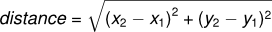
\includegraphics{distance_formula.png}
\end{quote}

The first step is to consider what a \code{distance} function should look like in
Python. In other words, what are the inputs (parameters) and what is the output
(return value)?

In this case, the two points are the inputs, which we can represent using four
parameters. The return value is the distance, which is a floating-point value.

Already we can write an outline of the function that captures our thinking so far:
\begin{quote}

\begin{Verbatim}[commandchars=\\\{\},numbers=left,firstnumber=1,stepnumber=1]
\PYG{k}{def} \PYG{n+nf}{distance}\PYG{p}{(}\PYG{n}{x1}\PYG{p}{,} \PYG{n}{y1}\PYG{p}{,} \PYG{n}{x2}\PYG{p}{,} \PYG{n}{y2}\PYG{p}{)}\PYG{p}{:}
    \PYG{k}{return} \PYG{l+m+mf}{0.0}
\end{Verbatim}
\end{quote}

Obviously, this version of the function doesn't compute distances; it always
returns zero. But it is syntactically correct, and it will run, which means
that we can test it before we make it more complicated.

To test the new function, we call it with sample values:
\begin{quote}

\begin{Verbatim}[commandchars=\\\{\}]
\PYG{g+gp}{\PYGZgt{}\PYGZgt{}\PYGZgt{} }\PYG{n}{distance}\PYG{p}{(}\PYG{l+m+mi}{1}\PYG{p}{,} \PYG{l+m+mi}{2}\PYG{p}{,} \PYG{l+m+mi}{4}\PYG{p}{,} \PYG{l+m+mi}{6}\PYG{p}{)}
\PYG{g+go}{0.0}
\end{Verbatim}
\end{quote}

We chose these values so that the horizontal distance equals 3 and the vertical
distance equals 4; that way, the result is 5 (the hypotenuse of a 3-4-5
triangle). When testing a function, it is useful to know the right answer.

At this point we have confirmed that the function is syntactically correct, and
we can start adding lines of code. After each incremental change, we test the
function again. If an error occurs at any point, we know where it must be --- in
the last line we added.

A logical first step in the computation is to find the differences
x$_{\text{2}}$- x$_{\text{1}}$ and y$_{\text{2}}$- y$_{\text{1}}$.  We will
refer to those values using temporary variables named \code{dx} and \code{dy}.
\begin{quote}

\begin{Verbatim}[commandchars=\\\{\},numbers=left,firstnumber=1,stepnumber=1]
\PYG{k}{def} \PYG{n+nf}{distance}\PYG{p}{(}\PYG{n}{x1}\PYG{p}{,} \PYG{n}{y1}\PYG{p}{,} \PYG{n}{x2}\PYG{p}{,} \PYG{n}{y2}\PYG{p}{)}\PYG{p}{:}
    \PYG{n}{dx} \PYG{o}{=} \PYG{n}{x2} \PYG{o}{-} \PYG{n}{x1}
    \PYG{n}{dy} \PYG{o}{=} \PYG{n}{y2} \PYG{o}{-} \PYG{n}{y1}
    \PYG{k}{return} \PYG{l+m+mf}{0.0}
\end{Verbatim}
\end{quote}

If we call the function with the arguments shown above, when the flow of execution
gets to the return statement, \code{dx} should be 3 and \code{dy} should be 4.
We can check that this is the case in \textbf{PyScripter} by putting the cursor on
the return statement, and running the program to break execution
when it gets to the cursor (using the \emph{F4} key).
Then we inspect the variables \code{dx} and \code{dy} by hovering the mouse above
them, to confirm that the function is getting the right parameters and performing the first
computation correctly. If not, there are only a few lines to check.

Next we compute the sum of squares of \code{dx} and \code{dy}:
\begin{quote}

\begin{Verbatim}[commandchars=\\\{\},numbers=left,firstnumber=1,stepnumber=1]
\PYG{k}{def} \PYG{n+nf}{distance}\PYG{p}{(}\PYG{n}{x1}\PYG{p}{,} \PYG{n}{y1}\PYG{p}{,} \PYG{n}{x2}\PYG{p}{,} \PYG{n}{y2}\PYG{p}{)}\PYG{p}{:}
    \PYG{n}{dx} \PYG{o}{=} \PYG{n}{x2} \PYG{o}{-} \PYG{n}{x1}
    \PYG{n}{dy} \PYG{o}{=} \PYG{n}{y2} \PYG{o}{-} \PYG{n}{y1}
    \PYG{n}{dsquared} \PYG{o}{=} \PYG{n}{dx}\PYG{o}{*}\PYG{n}{dx} \PYG{o}{+} \PYG{n}{dy}\PYG{o}{*}\PYG{n}{dy}
    \PYG{k}{return} \PYG{l+m+mf}{0.0}
\end{Verbatim}
\end{quote}

Again, we could run the program at this stage and check the value of \code{dsquared} (which
should be 25).

Finally, using the fractional exponent \code{0.5} to find the square root,
we compute and return the result:
\begin{quote}

\begin{Verbatim}[commandchars=\\\{\},numbers=left,firstnumber=1,stepnumber=1]
\PYG{k}{def} \PYG{n+nf}{distance}\PYG{p}{(}\PYG{n}{x1}\PYG{p}{,} \PYG{n}{y1}\PYG{p}{,} \PYG{n}{x2}\PYG{p}{,} \PYG{n}{y2}\PYG{p}{)}\PYG{p}{:}
    \PYG{n}{dx} \PYG{o}{=} \PYG{n}{x2} \PYG{o}{-} \PYG{n}{x1}
    \PYG{n}{dy} \PYG{o}{=} \PYG{n}{y2} \PYG{o}{-} \PYG{n}{y1}
    \PYG{n}{dsquared} \PYG{o}{=} \PYG{n}{dx}\PYG{o}{*}\PYG{n}{dx} \PYG{o}{+} \PYG{n}{dy}\PYG{o}{*}\PYG{n}{dy}
    \PYG{n}{result} \PYG{o}{=} \PYG{n}{dsquared}\PYG{o}{*}\PYG{o}{*}\PYG{l+m+mf}{0.5}
    \PYG{k}{return} \PYG{n}{result}
\end{Verbatim}
\end{quote}

If that works correctly, you are done. Otherwise, you might want to inspect the
value of \code{result} before the return statement.

When you start out, you might add only a line or two of code at a time. As you
gain more experience, you might find yourself writing and debugging bigger
conceptual chunks. Either way, stepping through your code one line at a time and
verifying that each step matches your expectations can save you a lot of
debugging time.  As you improve your programming skills you should find yourself
managing bigger and bigger chunks: this is very similar to the way we learned to read
letters, syllables, words, phrases, sentences, paragraphs, etc., or the way we learn
to chunk music --- from individual notes to chords, bars, phrases, and so on.

The key aspects of the process are:
\begin{enumerate}
\item {} 
Start with a working skeleton program and make small incremental changes. At any
point, if there is an error, you will know exactly where it is.

\item {} 
Use temporary variables to refer to intermediate values so that you
can easily inspect and check them.

\item {} 
Once the program is working, relax, sit back, and play around with your options.
(There is interesting research that links ``playfulness'' to better understanding,
better learning, more enjoyment, and a more positive mindset about
what you can achieve --- so spend some time fiddling around!)
You might want to consolidate multiple statements into one bigger compound expression,
or rename the variables you've used, or see if you can make the function shorter.
A good guideline is to aim for making code as easy as possible for others to read.

\end{enumerate}

Here is another version of the function.  It makes use of a square root function
that is in the \code{math} module (we'll learn about modules shortly).  Which do you
prefer?  Which looks ``closer'' to the Pythagorean formula we started out with?
\begin{quote}

\begin{Verbatim}[commandchars=\\\{\},numbers=left,firstnumber=1,stepnumber=1]
\PYG{k+kn}{import} \PYG{n+nn}{math}

\PYG{k}{def} \PYG{n+nf}{distance}\PYG{p}{(}\PYG{n}{x1}\PYG{p}{,} \PYG{n}{y1}\PYG{p}{,} \PYG{n}{x2}\PYG{p}{,} \PYG{n}{y2}\PYG{p}{)}\PYG{p}{:}
    \PYG{k}{return} \PYG{n}{math}\PYG{o}{.}\PYG{n}{sqrt}\PYG{p}{(} \PYG{p}{(}\PYG{n}{x2}\PYG{o}{-}\PYG{n}{x1}\PYG{p}{)}\PYG{o}{*}\PYG{o}{*}\PYG{l+m+mi}{2} \PYG{o}{+} \PYG{p}{(}\PYG{n}{y2}\PYG{o}{-}\PYG{n}{y1}\PYG{p}{)}\PYG{o}{*}\PYG{o}{*}\PYG{l+m+mi}{2} \PYG{p}{)}
\end{Verbatim}

\begin{Verbatim}[commandchars=\\\{\}]
\PYG{g+gp}{\PYGZgt{}\PYGZgt{}\PYGZgt{} }\PYG{n}{distance}\PYG{p}{(}\PYG{l+m+mi}{1}\PYG{p}{,} \PYG{l+m+mi}{2}\PYG{p}{,} \PYG{l+m+mi}{4}\PYG{p}{,} \PYG{l+m+mi}{6}\PYG{p}{)}
\PYG{g+go}{5.0}
\end{Verbatim}
\end{quote}

\index{debugging}

\section{Debugging with \texttt{print}}
\label{fruitful_functions:debugging-with-print}\label{fruitful_functions:index-3}
Another powerful technique for debugging (an alternative to single-stepping and
inspection of program variables), is to insert extra \code{print} functions
in carefully selected places in your code.  Then, by inspecting the output
of the program, you can check whether the algorithm is doing what you expect
it to.  Be clear about the following, however:
\begin{itemize}
\item {} 
You must have a clear solution to the problem, and must know what should
happen before you can debug a program.  Work on \emph{solving} the problem
on a piece of paper (perhaps using a flowchart to record the steps you take)
\emph{before} you concern yourself with
writing code.  Writing a program doesn't solve the problem --- it simply \emph{automates}
the manual steps you would take. So first make sure you have
a pen-and-paper manual solution that works.
Programming then is about making those manual steps happen automatically.

\item {} 
Do not write \textbf{chatterbox} functions.  A chatterbox is a fruitful
function that, in addition to its primary task, also asks the user for input,
or prints output, when it would be more useful
if it simply shut up and did its work quietly.

For example, we've seen built-in functions like \code{range},
\code{max} and \code{abs}.  None of these would be useful building blocks for other
programs if they prompted the user for input, or printed their results while
they performed their tasks.

So a good tip is to avoid calling \code{print} and \code{input} functions inside
fruitful functions, \emph{unless the primary purpose of your function is to
perform input and output}.  The one exception
to this rule might be to temporarily sprinkle some calls to \code{print} into
your code to help debug and understand what is happening when the code runs,
but these will then be removed once you get things working.

\end{itemize}

\index{composition}\index{function composition}

\section{Composition}
\label{fruitful_functions:index-4}\label{fruitful_functions:composition}
As you should expect by now, you can call one function from within another.
This ability is called \textbf{composition}.

As an example, we'll write a function that takes two points, the center of the
circle and a point on the perimeter, and computes the area of the circle.

Assume that the center point is stored in the variables \code{xc} and \code{yc}, and
the perimeter point is in \code{xp} and \code{yp}. The first step is to find the
radius of the circle, which is the distance between the two points.
Fortunately, we've just written a function, \code{distance}, that does just that,
so now all we have to do is use it:
\begin{quote}

\begin{Verbatim}[commandchars=\\\{\},numbers=left,firstnumber=1,stepnumber=1]
\PYG{n}{radius} \PYG{o}{=} \PYG{n}{distance}\PYG{p}{(}\PYG{n}{xc}\PYG{p}{,} \PYG{n}{yc}\PYG{p}{,} \PYG{n}{xp}\PYG{p}{,} \PYG{n}{yp}\PYG{p}{)}
\end{Verbatim}
\end{quote}

The second step is to find the area of a circle with that radius and return it.
Again we will use one of our earlier functions:
\begin{quote}

\begin{Verbatim}[commandchars=\\\{\},numbers=left,firstnumber=1,stepnumber=1]
\PYG{n}{result} \PYG{o}{=} \PYG{n}{area}\PYG{p}{(}\PYG{n}{radius}\PYG{p}{)}
\PYG{k}{return} \PYG{n}{result}
\end{Verbatim}
\end{quote}

Wrapping that up in a function, we get:
\begin{quote}

\begin{Verbatim}[commandchars=\\\{\},numbers=left,firstnumber=1,stepnumber=1]
\PYG{k}{def} \PYG{n+nf}{area2}\PYG{p}{(}\PYG{n}{xc}\PYG{p}{,} \PYG{n}{yc}\PYG{p}{,} \PYG{n}{xp}\PYG{p}{,} \PYG{n}{yp}\PYG{p}{)}\PYG{p}{:}
    \PYG{n}{radius} \PYG{o}{=} \PYG{n}{distance}\PYG{p}{(}\PYG{n}{xc}\PYG{p}{,} \PYG{n}{yc}\PYG{p}{,} \PYG{n}{xp}\PYG{p}{,} \PYG{n}{yp}\PYG{p}{)}
    \PYG{n}{result} \PYG{o}{=} \PYG{n}{area}\PYG{p}{(}\PYG{n}{radius}\PYG{p}{)}
    \PYG{k}{return} \PYG{n}{result}
\end{Verbatim}
\end{quote}

We called this function \code{area2} to distinguish it from the \code{area} function
defined earlier. There can only be one function with a given name within a
module.

The temporary variables \code{radius} and \code{result} are useful for development,
debugging, and single-stepping through the code to inspect what is happening,
but once the program is working, we can make it more concise by
composing the function calls:
\begin{quote}

\begin{Verbatim}[commandchars=\\\{\},numbers=left,firstnumber=1,stepnumber=1]
\PYG{k}{def} \PYG{n+nf}{area2}\PYG{p}{(}\PYG{n}{xc}\PYG{p}{,} \PYG{n}{yc}\PYG{p}{,} \PYG{n}{xp}\PYG{p}{,} \PYG{n}{yp}\PYG{p}{)}\PYG{p}{:}
    \PYG{k}{return} \PYG{n}{area}\PYG{p}{(}\PYG{n}{distance}\PYG{p}{(}\PYG{n}{xc}\PYG{p}{,} \PYG{n}{yc}\PYG{p}{,} \PYG{n}{xp}\PYG{p}{,} \PYG{n}{yp}\PYG{p}{)}\PYG{p}{)}
\end{Verbatim}
\end{quote}

\index{Boolean function}

\section{Boolean functions}
\label{fruitful_functions:index-5}\label{fruitful_functions:boolean-functions}
Functions can return Boolean values, which is often convenient for hiding
complicated tests inside functions. For example:
\begin{quote}

\begin{Verbatim}[commandchars=\\\{\},numbers=left,firstnumber=1,stepnumber=1]
\PYG{k}{def} \PYG{n+nf}{is\PYGZus{}divisible}\PYG{p}{(}\PYG{n}{x}\PYG{p}{,} \PYG{n}{y}\PYG{p}{)}\PYG{p}{:}
    \PYG{k}{if} \PYG{n}{x} \PYG{o}{\PYGZpc{}} \PYG{n}{y} \PYG{o}{==} \PYG{l+m+mi}{0}\PYG{p}{:}
        \PYG{k}{return} \PYG{k}{True}
    \PYG{k}{else}\PYG{p}{:}
        \PYG{k}{return} \PYG{k}{False}
\end{Verbatim}
\end{quote}

The name of this function is \code{is\_divisible}. It is common to give \textbf{Boolean
functions} names that sound like yes/no questions.  \code{is\_divisible} returns
either \code{True} or \code{False} to indicate whether the \code{x} is or is not
divisible by \code{y}.

We can make the function more concise by taking advantage of the fact that the
condition of the \code{if} statement is itself a Boolean expression. We can return
it directly, avoiding the \code{if} statement altogether:
\begin{quote}

\begin{Verbatim}[commandchars=\\\{\},numbers=left,firstnumber=1,stepnumber=1]
\PYG{k}{def} \PYG{n+nf}{is\PYGZus{}divisible}\PYG{p}{(}\PYG{n}{x}\PYG{p}{,} \PYG{n}{y}\PYG{p}{)}\PYG{p}{:}
    \PYG{k}{return} \PYG{n}{x} \PYG{o}{\PYGZpc{}} \PYG{n}{y} \PYG{o}{==} \PYG{l+m+mi}{0}
\end{Verbatim}
\end{quote}

This session shows the new function in action:
\begin{quote}

\begin{Verbatim}[commandchars=\\\{\}]
\PYG{g+gp}{\PYGZgt{}\PYGZgt{}\PYGZgt{} }\PYG{n}{is\PYGZus{}divisible}\PYG{p}{(}\PYG{l+m+mi}{6}\PYG{p}{,} \PYG{l+m+mi}{4}\PYG{p}{)}
\PYG{g+go}{False}
\PYG{g+gp}{\PYGZgt{}\PYGZgt{}\PYGZgt{} }\PYG{n}{is\PYGZus{}divisible}\PYG{p}{(}\PYG{l+m+mi}{6}\PYG{p}{,} \PYG{l+m+mi}{3}\PYG{p}{)}
\PYG{g+go}{True}
\end{Verbatim}
\end{quote}

Boolean functions are often used in conditional statements:
\begin{quote}

\begin{Verbatim}[commandchars=\\\{\},numbers=left,firstnumber=1,stepnumber=1]
\PYG{k}{if} \PYG{n}{is\PYGZus{}divisible}\PYG{p}{(}\PYG{n}{x}\PYG{p}{,} \PYG{n}{y}\PYG{p}{)}\PYG{p}{:}
    \PYG{o}{.}\PYG{o}{.}\PYG{o}{.} \PYG{c}{\PYGZsh{} Do something ...}
\PYG{k}{else}\PYG{p}{:}
    \PYG{o}{.}\PYG{o}{.}\PYG{o}{.} \PYG{c}{\PYGZsh{} Do something else ...}
\end{Verbatim}
\end{quote}

It might be tempting to write something like:
\begin{quote}

\begin{Verbatim}[commandchars=\\\{\},numbers=left,firstnumber=1,stepnumber=1]
\PYG{k}{if} \PYG{n}{is\PYGZus{}divisible}\PYG{p}{(}\PYG{n}{x}\PYG{p}{,} \PYG{n}{y}\PYG{p}{)} \PYG{o}{==} \PYG{k}{True}\PYG{p}{:}
\end{Verbatim}
\end{quote}

but the extra comparison is unnecessary.

\index{style}

\section{Programming with style}
\label{fruitful_functions:index-6}\label{fruitful_functions:programming-with-style}
Readability is very important to programmers, since in practice programs are
read and modified far more often then they are written.  But, like most rules,
we occasionaly break them.  Most of the code examples
in this book will be consistent with the \emph{Python Enhancement Proposal 8}
(\href{http://www.python.org/dev/peps/pep-0008/}{PEP 8}), a style guide developed by the Python community.

We'll have more to say about style as our programs become more complex, but a
few pointers will be helpful already:
\begin{itemize}
\item {} 
use 4 spaces (instead of tabs) for indentation

\item {} 
limit line length to 78 characters

\item {} 
when naming identifiers, use \code{CamelCase} for classes (we'll get to those)
and \code{lowercase\_with\_underscores} for functons and variables

\item {} 
place imports at the top of the file

\item {} 
keep function definitions together

\item {} 
use docstrings to document functions

\item {} 
use two blank lines to separate function definitions from each other

\item {} 
keep top level statements, including function calls, together at the
bottom of the program

\end{itemize}


\section{Unit testing}
\label{fruitful_functions:unit-testing}
It is a common best practice in software development these days to include
automatic \textbf{unit testing} of source code. Unit testing provides a way to
automatically verify that individual pieces of code, such as functions, are
working properly. This makes it possible to change the implementation of a
function at a later time and quickly test that it still does what it was
intended to do.

Unit testing also forces the programmer to think about the different cases
that the function needs to handle.  You also only have to type the tests once
into the script, rather than having to keep entering the same test data over
and over as you develop your code.

Extra code in your program which is there because it makes debugging or testing
easier is called \textbf{scaffolding}.

A collection of tests for some code is called its \textbf{test suite}.

There are a few different ways to do unit testing in Python ---
but at this stage we're going to ignore what the Python community usually does,
and we're going to start with two functions that we'll write ourselves.
We'll use these for writing our unit tests.

Let's start with the \code{absolute\_value} function that we wrote earlier in this
chapter.  Recall that we wrote a few different versions, the last of which was
incorrect, and had a bug. Would tests have caught this bug?

First we plan our tests.  We'd like to know
if the function returns the correct value when its argument is negative,
or when its argument is positive, or when its argument is zero.  When
planning your tests, you'll always want to think carefully about the ``edge'' cases ---
here, an argument of 0 to \code{absolute\_value} is on the edge of where the function
behaviour changes, and as we saw at the beginning of the chapter, it is an easy
spot for the programmer to make a mistake!  So it is a good case to include in
our test suite.

We're going to write a helper function for checking the results of one test.  It
takes two arguments --- the actual value that was
returned from the computation, and the value we expected to get.
It compares these, and will either print
a message telling us that the test passed, or it will print a message to
inform us that the test failed.  The first two lines of the body (after
the function's docstring) import a module called \code{sys}, and magically
determines the line number in the script where the call was made from.
This allows us to print the line number of the test, which will help
when we want to identify which tests have  passed or failed.
\begin{quote}

\begin{Verbatim}[commandchars=\\\{\},numbers=left,firstnumber=1,stepnumber=1]
\PYG{k+kn}{import} \PYG{n+nn}{sys}

\PYG{k}{def} \PYG{n+nf}{test}\PYG{p}{(}\PYG{n}{actual}\PYG{p}{,} \PYG{n}{expected}\PYG{p}{)}\PYG{p}{:}
    \PYG{l+s+sd}{""" Compare the actual to the expected value,}
\PYG{l+s+sd}{        and print a suitable message.}
\PYG{l+s+sd}{    """}
    \PYG{n}{linenum} \PYG{o}{=} \PYG{n}{sys}\PYG{o}{.}\PYG{n}{\PYGZus{}getframe}\PYG{p}{(}\PYG{l+m+mi}{1}\PYG{p}{)}\PYG{o}{.}\PYG{n}{f\PYGZus{}lineno}   \PYG{c}{\PYGZsh{} Get the caller's line number.}
    \PYG{k}{if} \PYG{p}{(}\PYG{n}{expected} \PYG{o}{==} \PYG{n}{actual}\PYG{p}{)}\PYG{p}{:}
        \PYG{n}{msg} \PYG{o}{=} \PYG{l+s}{"}\PYG{l+s}{Test on line \PYGZob{}0\PYGZcb{} passed.}\PYG{l+s}{"}\PYG{o}{.}\PYG{n}{format}\PYG{p}{(}\PYG{n}{linenum}\PYG{p}{)}
    \PYG{k}{else}\PYG{p}{:}
        \PYG{n}{msg} \PYG{o}{=} \PYG{p}{(}\PYG{l+s}{"}\PYG{l+s}{Test on line \PYGZob{}0\PYGZcb{} failed. Expected }\PYG{l+s}{'}\PYG{l+s}{\PYGZob{}1\PYGZcb{}}\PYG{l+s}{'}\PYG{l+s}{, but got }\PYG{l+s}{'}\PYG{l+s}{\PYGZob{}2\PYGZcb{}}\PYG{l+s}{'}\PYG{l+s}{.}\PYG{l+s}{"}
                \PYG{o}{.}\PYG{n}{format}\PYG{p}{(}\PYG{n}{linenum}\PYG{p}{,} \PYG{n}{expected}\PYG{p}{,} \PYG{n}{actual}\PYG{p}{)}\PYG{p}{)}
    \PYG{n+nb}{print}\PYG{p}{(}\PYG{n}{msg}\PYG{p}{)}
\end{Verbatim}
\end{quote}

There is also some slightly tricky string formatting using the \code{format} method
which we will gloss over for the moment, and cover in detail in a future chapter.
But with this function written, we can proceed to construct our test suite:
\begin{quote}

\begin{Verbatim}[commandchars=\\\{\}]
\PYG{k}{def} \PYG{n+nf}{test\PYGZus{}suite}\PYG{p}{(}\PYG{p}{)}\PYG{p}{:}
    \PYG{l+s+sd}{""" Run the suite of tests for code in this module (this file).}
\PYG{l+s+sd}{    """}
    \PYG{n}{test}\PYG{p}{(}\PYG{n}{absolute\PYGZus{}value}\PYG{p}{(}\PYG{l+m+mi}{17}\PYG{p}{)}\PYG{p}{,} \PYG{l+m+mi}{17}\PYG{p}{)}
    \PYG{n}{test}\PYG{p}{(}\PYG{n}{absolute\PYGZus{}value}\PYG{p}{(}\PYG{o}{-}\PYG{l+m+mi}{17}\PYG{p}{)}\PYG{p}{,} \PYG{l+m+mi}{17}\PYG{p}{)}
    \PYG{n}{test}\PYG{p}{(}\PYG{n}{absolute\PYGZus{}value}\PYG{p}{(}\PYG{l+m+mi}{0}\PYG{p}{)}\PYG{p}{,} \PYG{l+m+mi}{0}\PYG{p}{)}
    \PYG{n}{test}\PYG{p}{(}\PYG{n}{absolute\PYGZus{}value}\PYG{p}{(}\PYG{l+m+mf}{3.14}\PYG{p}{)}\PYG{p}{,} \PYG{l+m+mf}{3.14}\PYG{p}{)}
    \PYG{n}{test}\PYG{p}{(}\PYG{n}{absolute\PYGZus{}value}\PYG{p}{(}\PYG{o}{-}\PYG{l+m+mf}{3.14}\PYG{p}{)}\PYG{p}{,} \PYG{l+m+mf}{3.14}\PYG{p}{)}

\PYG{n}{test\PYGZus{}suite}\PYG{p}{(}\PYG{p}{)}        \PYG{c}{\PYGZsh{} Here is the call to run the tests}
\end{Verbatim}
\end{quote}

Here you'll see that we've constructed five tests in our test suite.  We could run this
against the first or second versions (the correct versions) of \code{absolute\_value},
and we'd get output similar to the following:
\begin{quote}

\begin{Verbatim}[commandchars=\\\{\}]
\PYG{g+go}{Test on line 24 passed.}
\PYG{g+go}{Test on line 25 passed.}
\PYG{g+go}{Test on line 26 passed.}
\PYG{g+go}{Test on line 27 passed.}
\PYG{g+go}{Test on line 28 passed.}
\end{Verbatim}
\end{quote}

But let's say you change the function to an incorrect version like this:
\begin{quote}

\begin{Verbatim}[commandchars=\\\{\},numbers=left,firstnumber=1,stepnumber=1]
\PYG{k}{def} \PYG{n+nf}{absolute\PYGZus{}value}\PYG{p}{(}\PYG{n}{n}\PYG{p}{)}\PYG{p}{:}   \PYG{c}{\PYGZsh{} Buggy version}
    \PYG{l+s+sd}{""" Compute the absolute value of n """}
    \PYG{k}{if} \PYG{n}{n} \PYG{o}{\PYGZlt{}} \PYG{l+m+mi}{0}\PYG{p}{:}
        \PYG{k}{return} \PYG{l+m+mi}{1}
    \PYG{k}{elif} \PYG{n}{n} \PYG{o}{\PYGZgt{}} \PYG{l+m+mi}{0}\PYG{p}{:}
        \PYG{k}{return} \PYG{n}{n}
\end{Verbatim}
\end{quote}

Can you find at least two mistakes in this code?  Our test suite can!  We get:

\begin{Verbatim}[commandchars=\\\{\}]
Test on line 24 passed.
Test on line 25 failed. Expected '17', but got '1'.
Test on line 26 failed. Expected '0', but got 'None'.
Test on line 27 passed.
Test on line 28 failed. Expected '3.14', but got '1'.
\end{Verbatim}

These are three examples of \emph{failing tests}.


\section{Glossary}
\label{fruitful_functions:glossary}\begin{description}
\item[{\index{Boolean function|textbf}Boolean function}] \leavevmode\phantomsection\label{fruitful_functions:term-boolean-function}
A function that returns a Boolean value.  The only possible
values of the \code{bool} type are \code{False} and \code{True}.

\item[{\index{chatterbox function|textbf}chatterbox function}] \leavevmode\phantomsection\label{fruitful_functions:term-chatterbox-function}
A function which interacts with the user (using \code{input} or \code{print}) when
it should not. Silent functions that just convert their input arguments into
their output results are usually the most useful ones.

\item[{\index{composition (of functions)|textbf}composition (of functions)}] \leavevmode\phantomsection\label{fruitful_functions:term-composition-of-functions}
Calling one function from within the body of another, or using the
return value of one function as an argument to the call of another.

\item[{\index{dead code|textbf}dead code}] \leavevmode\phantomsection\label{fruitful_functions:term-dead-code}
Part of a program that can never be executed, often because it appears
after a \code{return} statement.

\item[{\index{fruitful function|textbf}fruitful function}] \leavevmode\phantomsection\label{fruitful_functions:term-fruitful-function}
A function that yields a return value instead of \code{None}.

\item[{\index{incremental development|textbf}incremental development}] \leavevmode\phantomsection\label{fruitful_functions:term-incremental-development}
A program development plan intended to simplify debugging by adding and
testing only a small amount of code at a time.

\item[{\index{None|textbf}None}] \leavevmode\phantomsection\label{fruitful_functions:term-none}
A special Python value. One use in Python is that it is returned
by functions that do not execute a return statement with a return argument.

\item[{\index{return value|textbf}return value}] \leavevmode\phantomsection\label{fruitful_functions:term-return-value}
The value provided as the result of a function call.

\item[{\index{scaffolding|textbf}scaffolding}] \leavevmode\phantomsection\label{fruitful_functions:term-scaffolding}
Code that is used during program development to assist with development
and debugging. The unit test code that we added in this chapter are
examples of scaffolding.

\item[{\index{temporary variable|textbf}temporary variable}] \leavevmode\phantomsection\label{fruitful_functions:term-temporary-variable}
A variable used to store an intermediate value in a complex
calculation.

\item[{\index{test suite|textbf}test suite}] \leavevmode\phantomsection\label{fruitful_functions:term-test-suite}
A collection of tests for some code you have written.

\item[{\index{unit testing|textbf}unit testing}] \leavevmode\phantomsection\label{fruitful_functions:term-unit-testing}
An automatic procedure used to validate that individual units of code
are working properly.  Having a test suite is extremely useful when somebody
modifies or extends the code: it provides a safety net against
going backwards by putting new bugs into previously working code.
The term \emph{regression} testing is often used to capture this idea that we
don't want to go backwards!

\end{description}


\section{Exercises}
\label{fruitful_functions:exercises}
All of the exercises below should be added to a single file.  In that file, you should
also add the \code{test} and \code{test\_suite} scaffolding functions shown above, and then,
as you work through the exercises, add the new tests to your test suite.
(If you open the online version of the textbook,
you can easily copy and paste the tests and the fragments of code into your Python editor.)

After completing each exercise, confirm that all the tests pass.
\begin{enumerate}
\item {} 
The four compass points can be abbreviated by single-letter strings as ``N'', ``E'', ``S'', and ``W''.
Write a function \code{turn\_clockwise} that takes one of these four compass points as
its parameter, and returns the next compass point in the clockwise direction.
Here are some tests that should pass:

\begin{Verbatim}[commandchars=\\\{\}]
\PYG{n}{test}\PYG{p}{(}\PYG{n}{turn\PYGZus{}clockwise}\PYG{p}{(}\PYG{l+s}{"}\PYG{l+s}{N}\PYG{l+s}{"}\PYG{p}{)}\PYG{p}{,} \PYG{l+s}{"}\PYG{l+s}{E}\PYG{l+s}{"}\PYG{p}{)}
\PYG{n}{test}\PYG{p}{(}\PYG{n}{turn\PYGZus{}clockwise}\PYG{p}{(}\PYG{l+s}{"}\PYG{l+s}{W}\PYG{l+s}{"}\PYG{p}{)}\PYG{p}{,} \PYG{l+s}{"}\PYG{l+s}{N}\PYG{l+s}{"}\PYG{p}{)}
\end{Verbatim}

You might ask \emph{``What if the argument to the function is some other value?''}  For all
other cases, the function should return the value \code{None}:

\begin{Verbatim}[commandchars=\\\{\}]
\PYG{n}{test}\PYG{p}{(}\PYG{n}{turn\PYGZus{}clockwise}\PYG{p}{(}\PYG{l+m+mi}{42}\PYG{p}{)}\PYG{p}{,} \PYG{n+nb+bp}{None}\PYG{p}{)}
\PYG{n}{test}\PYG{p}{(}\PYG{n}{turn\PYGZus{}clockwise}\PYG{p}{(}\PYG{l+s}{"}\PYG{l+s}{rubbish}\PYG{l+s}{"}\PYG{p}{)}\PYG{p}{,} \PYG{n+nb+bp}{None}\PYG{p}{)}
\end{Verbatim}

\item {} 
Write a function \code{day\_name} that converts an integer number 0 to 6 into the name of
a day.  Assume day 0 is ``Sunday''.  Once again, return None if the arguments to the function
are not valid.  Here are some tests that should pass:

\begin{Verbatim}[commandchars=\\\{\}]
\PYG{n}{test}\PYG{p}{(}\PYG{n}{day\PYGZus{}name}\PYG{p}{(}\PYG{l+m+mi}{3}\PYG{p}{)}\PYG{p}{,} \PYG{l+s}{"}\PYG{l+s}{Wednesday}\PYG{l+s}{"}\PYG{p}{)}
\PYG{n}{test}\PYG{p}{(}\PYG{n}{day\PYGZus{}name}\PYG{p}{(}\PYG{l+m+mi}{6}\PYG{p}{)}\PYG{p}{,} \PYG{l+s}{"}\PYG{l+s}{Saturday}\PYG{l+s}{"}\PYG{p}{)}
\PYG{n}{test}\PYG{p}{(}\PYG{n}{day\PYGZus{}name}\PYG{p}{(}\PYG{l+m+mi}{42}\PYG{p}{)}\PYG{p}{,} \PYG{n+nb+bp}{None}\PYG{p}{)}
\end{Verbatim}

\item {} 
Write the inverse function \code{day\_num} which is given a day name, and returns its number:

\begin{Verbatim}[commandchars=\\\{\}]
\PYG{n}{test}\PYG{p}{(}\PYG{n}{day\PYGZus{}num}\PYG{p}{(}\PYG{l+s}{"}\PYG{l+s}{Friday}\PYG{l+s}{"}\PYG{p}{)}\PYG{p}{,} \PYG{l+m+mi}{5}\PYG{p}{)}
\PYG{n}{test}\PYG{p}{(}\PYG{n}{day\PYGZus{}num}\PYG{p}{(}\PYG{l+s}{"}\PYG{l+s}{Sunday}\PYG{l+s}{"}\PYG{p}{)}\PYG{p}{,} \PYG{l+m+mi}{0}\PYG{p}{)}
\PYG{n}{test}\PYG{p}{(}\PYG{n}{day\PYGZus{}num}\PYG{p}{(}\PYG{n}{day\PYGZus{}name}\PYG{p}{(}\PYG{l+m+mi}{3}\PYG{p}{)}\PYG{p}{)}\PYG{p}{,} \PYG{l+m+mi}{3}\PYG{p}{)}
\PYG{n}{test}\PYG{p}{(}\PYG{n}{day\PYGZus{}name}\PYG{p}{(}\PYG{n}{day\PYGZus{}num}\PYG{p}{(}\PYG{l+s}{"}\PYG{l+s}{Thursday}\PYG{l+s}{"}\PYG{p}{)}\PYG{p}{)}\PYG{p}{,} \PYG{l+s}{"}\PYG{l+s}{Thursday}\PYG{l+s}{"}\PYG{p}{)}
\end{Verbatim}

Once again, if this function is given an invalid argument, it should return \code{None}:

\begin{Verbatim}[commandchars=\\\{\}]
\PYG{n}{test}\PYG{p}{(}\PYG{n}{day\PYGZus{}num}\PYG{p}{(}\PYG{l+s}{"}\PYG{l+s}{Halloween}\PYG{l+s}{"}\PYG{p}{)}\PYG{p}{,} \PYG{n+nb+bp}{None}\PYG{p}{)}
\end{Verbatim}

\item {} 
Write a function that helps answer questions like ```Today is Wednesday.  I leave on holiday
in 19 days time.  What day will that be?''' So the function must take a day name and
a \code{delta} argument --- the number of days to add --- and should return the resulting day name:

\begin{Verbatim}[commandchars=\\\{\}]
\PYG{n}{test}\PYG{p}{(}\PYG{n}{day\PYGZus{}add}\PYG{p}{(}\PYG{l+s}{"}\PYG{l+s}{Monday}\PYG{l+s}{"}\PYG{p}{,} \PYG{l+m+mi}{4}\PYG{p}{)}\PYG{p}{,}  \PYG{l+s}{"}\PYG{l+s}{Friday}\PYG{l+s}{"}\PYG{p}{)}
\PYG{n}{test}\PYG{p}{(}\PYG{n}{day\PYGZus{}add}\PYG{p}{(}\PYG{l+s}{"}\PYG{l+s}{Tuesday}\PYG{l+s}{"}\PYG{p}{,} \PYG{l+m+mi}{0}\PYG{p}{)}\PYG{p}{,} \PYG{l+s}{"}\PYG{l+s}{Tuesday}\PYG{l+s}{"}\PYG{p}{)}
\PYG{n}{test}\PYG{p}{(}\PYG{n}{day\PYGZus{}add}\PYG{p}{(}\PYG{l+s}{"}\PYG{l+s}{Tuesday}\PYG{l+s}{"}\PYG{p}{,} \PYG{l+m+mi}{14}\PYG{p}{)}\PYG{p}{,} \PYG{l+s}{"}\PYG{l+s}{Tuesday}\PYG{l+s}{"}\PYG{p}{)}
\PYG{n}{test}\PYG{p}{(}\PYG{n}{day\PYGZus{}add}\PYG{p}{(}\PYG{l+s}{"}\PYG{l+s}{Sunday}\PYG{l+s}{"}\PYG{p}{,} \PYG{l+m+mi}{100}\PYG{p}{)}\PYG{p}{,} \PYG{l+s}{"}\PYG{l+s}{Tuesday}\PYG{l+s}{"}\PYG{p}{)}
\end{Verbatim}

\emph{Hint: use the first two functions written above to help you write this one.}

\item {} 
Can your \code{day\_add} function already work with negative deltas? For example,
-1 would be yesterday, or -7 would be a week ago:

\begin{Verbatim}[commandchars=\\\{\}]
\PYG{n}{test}\PYG{p}{(}\PYG{n}{day\PYGZus{}add}\PYG{p}{(}\PYG{l+s}{"}\PYG{l+s}{Sunday}\PYG{l+s}{"}\PYG{p}{,} \PYG{o}{-}\PYG{l+m+mi}{1}\PYG{p}{)}\PYG{p}{,} \PYG{l+s}{"}\PYG{l+s}{Saturday}\PYG{l+s}{"}\PYG{p}{)}
\PYG{n}{test}\PYG{p}{(}\PYG{n}{day\PYGZus{}add}\PYG{p}{(}\PYG{l+s}{"}\PYG{l+s}{Sunday}\PYG{l+s}{"}\PYG{p}{,} \PYG{o}{-}\PYG{l+m+mi}{7}\PYG{p}{)}\PYG{p}{,} \PYG{l+s}{"}\PYG{l+s}{Sunday}\PYG{l+s}{"}\PYG{p}{)}
\PYG{n}{test}\PYG{p}{(}\PYG{n}{day\PYGZus{}add}\PYG{p}{(}\PYG{l+s}{"}\PYG{l+s}{Tuesday}\PYG{l+s}{"}\PYG{p}{,} \PYG{o}{-}\PYG{l+m+mi}{100}\PYG{p}{)}\PYG{p}{,} \PYG{l+s}{"}\PYG{l+s}{Sunday}\PYG{l+s}{"}\PYG{p}{)}
\end{Verbatim}

If your function already works, explain why.  If it does not work, make it work.

\emph{Hint:} Play with some cases of using the modulus function \emph{\%}
(introduced at the beginning of the previous chapter).  Specifically, explore
what happens to  \code{x \% 7}  when x is negative.

\item {} 
Write a function \code{days\_in\_month} which takes the name of a month, and returns the number
of days in the month.  Ignore leap years:

\begin{Verbatim}[commandchars=\\\{\}]
\PYG{n}{test}\PYG{p}{(}\PYG{n}{days\PYGZus{}in\PYGZus{}month}\PYG{p}{(}\PYG{l+s}{"}\PYG{l+s}{February}\PYG{l+s}{"}\PYG{p}{)}\PYG{p}{,} \PYG{l+m+mi}{28}\PYG{p}{)}
\PYG{n}{test}\PYG{p}{(}\PYG{n}{days\PYGZus{}in\PYGZus{}month}\PYG{p}{(}\PYG{l+s}{"}\PYG{l+s}{December}\PYG{l+s}{"}\PYG{p}{)}\PYG{p}{,} \PYG{l+m+mi}{31}\PYG{p}{)}
\end{Verbatim}

If the function is given invalid arguments, it should return \code{None}.

\item {} 
Write a function \code{to\_secs} that converts hours, minutes and seconds to
a total number of seconds.  Here are some tests that should pass:

\begin{Verbatim}[commandchars=\\\{\}]
\PYG{n}{test}\PYG{p}{(}\PYG{n}{to\PYGZus{}secs}\PYG{p}{(}\PYG{l+m+mi}{2}\PYG{p}{,} \PYG{l+m+mi}{30}\PYG{p}{,} \PYG{l+m+mi}{10}\PYG{p}{)}\PYG{p}{,} \PYG{l+m+mi}{9010}\PYG{p}{)}
\PYG{n}{test}\PYG{p}{(}\PYG{n}{to\PYGZus{}secs}\PYG{p}{(}\PYG{l+m+mi}{2}\PYG{p}{,} \PYG{l+m+mi}{0}\PYG{p}{,} \PYG{l+m+mi}{0}\PYG{p}{)}\PYG{p}{,} \PYG{l+m+mi}{7200}\PYG{p}{)}
\PYG{n}{test}\PYG{p}{(}\PYG{n}{to\PYGZus{}secs}\PYG{p}{(}\PYG{l+m+mi}{0}\PYG{p}{,} \PYG{l+m+mi}{2}\PYG{p}{,} \PYG{l+m+mi}{0}\PYG{p}{)}\PYG{p}{,} \PYG{l+m+mi}{120}\PYG{p}{)}
\PYG{n}{test}\PYG{p}{(}\PYG{n}{to\PYGZus{}secs}\PYG{p}{(}\PYG{l+m+mi}{0}\PYG{p}{,} \PYG{l+m+mi}{0}\PYG{p}{,} \PYG{l+m+mi}{42}\PYG{p}{)}\PYG{p}{,} \PYG{l+m+mi}{42}\PYG{p}{)}
\PYG{n}{test}\PYG{p}{(}\PYG{n}{to\PYGZus{}secs}\PYG{p}{(}\PYG{l+m+mi}{0}\PYG{p}{,} \PYG{o}{-}\PYG{l+m+mi}{10}\PYG{p}{,} \PYG{l+m+mi}{10}\PYG{p}{)}\PYG{p}{,} \PYG{o}{-}\PYG{l+m+mi}{590}\PYG{p}{)}
\end{Verbatim}

\item {} 
Extend \code{to\_secs} so that it can cope with real values as inputs.  It
should always return an integer number of seconds (truncated towards zero):

\begin{Verbatim}[commandchars=\\\{\}]
\PYG{n}{test}\PYG{p}{(}\PYG{n}{to\PYGZus{}secs}\PYG{p}{(}\PYG{l+m+mf}{2.5}\PYG{p}{,} \PYG{l+m+mi}{0}\PYG{p}{,} \PYG{l+m+mf}{10.71}\PYG{p}{)}\PYG{p}{,} \PYG{l+m+mi}{9010}\PYG{p}{)}
\PYG{n}{test}\PYG{p}{(}\PYG{n}{to\PYGZus{}secs}\PYG{p}{(}\PYG{l+m+mf}{2.433}\PYG{p}{,}\PYG{l+m+mi}{0}\PYG{p}{,}\PYG{l+m+mi}{0}\PYG{p}{)}\PYG{p}{,} \PYG{l+m+mi}{8758}\PYG{p}{)}
\end{Verbatim}

\item {} 
Write three functions that are the ``inverses'' of \code{to\_secs}:
\begin{enumerate}
\item {} 
\code{hours\_in} returns the whole integer number of hours
represented by a total number of seconds.

\item {} 
\code{minutes\_in} returns the whole integer number of left over minutes
in a total number of seconds, once the hours
have been taken out.

\item {} 
\code{seconds\_in} returns the left over seconds
represented by a total number of seconds.

\end{enumerate}

You may assume that the total number of seconds passed to these functions is an integer.
Here are some test cases:

\begin{Verbatim}[commandchars=\\\{\}]
\PYG{n}{test}\PYG{p}{(}\PYG{n}{hours\PYGZus{}in}\PYG{p}{(}\PYG{l+m+mi}{9010}\PYG{p}{)}\PYG{p}{,} \PYG{l+m+mi}{2}\PYG{p}{)}
\PYG{n}{test}\PYG{p}{(}\PYG{n}{minutes\PYGZus{}in}\PYG{p}{(}\PYG{l+m+mi}{9010}\PYG{p}{)}\PYG{p}{,} \PYG{l+m+mi}{30}\PYG{p}{)}
\PYG{n}{test}\PYG{p}{(}\PYG{n}{seconds\PYGZus{}in}\PYG{p}{(}\PYG{l+m+mi}{9010}\PYG{p}{)}\PYG{p}{,} \PYG{l+m+mi}{10}\PYG{p}{)}
\end{Verbatim}

\begin{notice}{note}{It won't always be obvious what is wanted ...}

In the third case above, the requirement seems quite ambiguous and fuzzy.  But the test clarifies
what we actually need to do.

Unit tests often have this secondary benefit of clarifying the specifications.   If you write your
own test suites, consider it part of the problem-solving process as you ask questions about what
you really expect to happen, and whether you've considered all the possible cases.

Since our book is titled \emph{How to Think Like ...} you might enjoy reading at least one reference about
thinking, and about fun ideas like \emph{fluid intelligence}, a key ingredient in problem solving.
See, for example, \href{http://psychology.about.com/od/cognitivepsychology/a/fluid-crystal.htm}{http://psychology.about.com/od/cognitivepsychology/a/fluid-crystal.htm}.
Learning Computer Science requires a good mix of both fluid and crystallized kinds of intelligence.
\end{notice}

\item {} 
Which of these tests fail?  Explain why.

\begin{Verbatim}[commandchars=\\\{\}]
\PYG{n}{test}\PYG{p}{(}\PYG{l+m+mi}{3} \PYG{o}{\PYGZpc{}} \PYG{l+m+mi}{4}\PYG{p}{,} \PYG{l+m+mi}{0}\PYG{p}{)}
\PYG{n}{test}\PYG{p}{(}\PYG{l+m+mi}{3} \PYG{o}{\PYGZpc{}} \PYG{l+m+mi}{4}\PYG{p}{,} \PYG{l+m+mi}{3}\PYG{p}{)}
\PYG{n}{test}\PYG{p}{(}\PYG{l+m+mi}{3} \PYG{o}{/} \PYG{l+m+mi}{4}\PYG{p}{,} \PYG{l+m+mi}{0}\PYG{p}{)}
\PYG{n}{test}\PYG{p}{(}\PYG{l+m+mi}{3} \PYG{o}{/}\PYG{o}{/} \PYG{l+m+mi}{4}\PYG{p}{,} \PYG{l+m+mi}{0}\PYG{p}{)}
\PYG{n}{test}\PYG{p}{(}\PYG{l+m+mi}{3}\PYG{o}{+}\PYG{l+m+mi}{4}  \PYG{o}{*}  \PYG{l+m+mi}{2}\PYG{p}{,} \PYG{l+m+mi}{14}\PYG{p}{)}
\PYG{n}{test}\PYG{p}{(}\PYG{l+m+mi}{4}\PYG{o}{-}\PYG{l+m+mi}{2}\PYG{o}{+}\PYG{l+m+mi}{2}\PYG{p}{,} \PYG{l+m+mi}{0}\PYG{p}{)}
\PYG{n}{test}\PYG{p}{(}\PYG{n+nb}{len}\PYG{p}{(}\PYG{l+s}{"}\PYG{l+s}{hello, world!}\PYG{l+s}{"}\PYG{p}{)}\PYG{p}{,} \PYG{l+m+mi}{13}\PYG{p}{)}
\end{Verbatim}

\item {} 
Write a \code{compare} function that returns \code{1} if \code{a \textgreater{} b}, \code{0} if
\code{a == b}, and \code{-1} if \code{a \textless{} b}

\begin{Verbatim}[commandchars=\\\{\}]
\PYG{n}{test}\PYG{p}{(}\PYG{n}{compare}\PYG{p}{(}\PYG{l+m+mi}{5}\PYG{p}{,} \PYG{l+m+mi}{4}\PYG{p}{)}\PYG{p}{,} \PYG{l+m+mi}{1}\PYG{p}{)}
\PYG{n}{test}\PYG{p}{(}\PYG{n}{compare}\PYG{p}{(}\PYG{l+m+mi}{7}\PYG{p}{,} \PYG{l+m+mi}{7}\PYG{p}{)}\PYG{p}{,} \PYG{l+m+mi}{0}\PYG{p}{)}
\PYG{n}{test}\PYG{p}{(}\PYG{n}{compare}\PYG{p}{(}\PYG{l+m+mi}{2}\PYG{p}{,} \PYG{l+m+mi}{3}\PYG{p}{)}\PYG{p}{,} \PYG{o}{-}\PYG{l+m+mi}{1}\PYG{p}{)}
\PYG{n}{test}\PYG{p}{(}\PYG{n}{compare}\PYG{p}{(}\PYG{l+m+mi}{42}\PYG{p}{,} \PYG{l+m+mi}{1}\PYG{p}{)}\PYG{p}{,} \PYG{l+m+mi}{1}\PYG{p}{)}
\end{Verbatim}

\item {} 
Write a function called \code{hypotenuse} that
returns the length of the hypotenuse of a right triangle given the lengths
of the two legs as parameters:

\begin{Verbatim}[commandchars=\\\{\}]
\PYG{n}{test}\PYG{p}{(}\PYG{n}{hypotenuse}\PYG{p}{(}\PYG{l+m+mi}{3}\PYG{p}{,} \PYG{l+m+mi}{4}\PYG{p}{)}\PYG{p}{,} \PYG{l+m+mf}{5.0}\PYG{p}{)}
\PYG{n}{test}\PYG{p}{(}\PYG{n}{hypotenuse}\PYG{p}{(}\PYG{l+m+mi}{12}\PYG{p}{,} \PYG{l+m+mi}{5}\PYG{p}{)}\PYG{p}{,} \PYG{l+m+mf}{13.0}\PYG{p}{)}
\PYG{n}{test}\PYG{p}{(}\PYG{n}{hypotenuse}\PYG{p}{(}\PYG{l+m+mi}{24}\PYG{p}{,} \PYG{l+m+mi}{7}\PYG{p}{)}\PYG{p}{,} \PYG{l+m+mf}{25.0}\PYG{p}{)}
\PYG{n}{test}\PYG{p}{(}\PYG{n}{hypotenuse}\PYG{p}{(}\PYG{l+m+mi}{9}\PYG{p}{,} \PYG{l+m+mi}{12}\PYG{p}{)}\PYG{p}{,} \PYG{l+m+mf}{15.0}\PYG{p}{)}
\end{Verbatim}

\item {} 
Write a function \code{slope(x1, y1, x2, y2)} that returns the slope of
the line through the points (x1, y1) and (x2, y2). Be sure your
implementation of \code{slope} can pass the following tests:

\begin{Verbatim}[commandchars=\\\{\}]
\PYG{n}{test}\PYG{p}{(}\PYG{n}{slope}\PYG{p}{(}\PYG{l+m+mi}{5}\PYG{p}{,} \PYG{l+m+mi}{3}\PYG{p}{,} \PYG{l+m+mi}{4}\PYG{p}{,} \PYG{l+m+mi}{2}\PYG{p}{)}\PYG{p}{,} \PYG{l+m+mf}{1.0}\PYG{p}{)}
\PYG{n}{test}\PYG{p}{(}\PYG{n}{slope}\PYG{p}{(}\PYG{l+m+mi}{1}\PYG{p}{,} \PYG{l+m+mi}{2}\PYG{p}{,} \PYG{l+m+mi}{3}\PYG{p}{,} \PYG{l+m+mi}{2}\PYG{p}{)}\PYG{p}{,} \PYG{l+m+mf}{0.0}\PYG{p}{)}
\PYG{n}{test}\PYG{p}{(}\PYG{n}{slope}\PYG{p}{(}\PYG{l+m+mi}{1}\PYG{p}{,} \PYG{l+m+mi}{2}\PYG{p}{,} \PYG{l+m+mi}{3}\PYG{p}{,} \PYG{l+m+mi}{3}\PYG{p}{)}\PYG{p}{,} \PYG{l+m+mf}{0.5}\PYG{p}{)}
\PYG{n}{test}\PYG{p}{(}\PYG{n}{slope}\PYG{p}{(}\PYG{l+m+mi}{2}\PYG{p}{,} \PYG{l+m+mi}{4}\PYG{p}{,} \PYG{l+m+mi}{1}\PYG{p}{,} \PYG{l+m+mi}{2}\PYG{p}{)}\PYG{p}{,} \PYG{l+m+mf}{2.0}\PYG{p}{)}
\end{Verbatim}

Then use a call to \code{slope} in a new function named
\code{intercept(x1, y1, x2, y2)} that returns the y-intercept of the line
through the points \code{(x1, y1)} and \code{(x2, y2)}

\begin{Verbatim}[commandchars=\\\{\}]
\PYG{n}{test}\PYG{p}{(}\PYG{n}{intercept}\PYG{p}{(}\PYG{l+m+mi}{1}\PYG{p}{,} \PYG{l+m+mi}{6}\PYG{p}{,} \PYG{l+m+mi}{3}\PYG{p}{,} \PYG{l+m+mi}{12}\PYG{p}{)}\PYG{p}{,} \PYG{l+m+mf}{3.0}\PYG{p}{)}
\PYG{n}{test}\PYG{p}{(}\PYG{n}{intercept}\PYG{p}{(}\PYG{l+m+mi}{6}\PYG{p}{,} \PYG{l+m+mi}{1}\PYG{p}{,} \PYG{l+m+mi}{1}\PYG{p}{,} \PYG{l+m+mi}{6}\PYG{p}{)}\PYG{p}{,} \PYG{l+m+mf}{7.0}\PYG{p}{)}
\PYG{n}{test}\PYG{p}{(}\PYG{n}{intercept}\PYG{p}{(}\PYG{l+m+mi}{4}\PYG{p}{,} \PYG{l+m+mi}{6}\PYG{p}{,} \PYG{l+m+mi}{12}\PYG{p}{,} \PYG{l+m+mi}{8}\PYG{p}{)}\PYG{p}{,} \PYG{l+m+mf}{5.0}\PYG{p}{)}
\end{Verbatim}

\item {} 
Write a function called \code{is\_even(n)} that takes an integer as an argument
and returns \code{True} if the argument is an \textbf{even number} and \code{False} if
it is \textbf{odd}.

Add your own tests to the test suite.

\item {} 
Now write the function \code{is\_odd(n)} that returns \code{True} when \code{n} is odd
and \code{False} otherwise. Include unit tests for this function too.

Finally, modify it so that it uses a call to \code{is\_even} to determine if its
argument is an odd integer, and ensure that its test still pass.

\item {} 
Write a function \code{is\_factor(f, n)} that passes these tests:

\begin{Verbatim}[commandchars=\\\{\}]
\PYG{n}{test}\PYG{p}{(}\PYG{n}{is\PYGZus{}factor}\PYG{p}{(}\PYG{l+m+mi}{3}\PYG{p}{,} \PYG{l+m+mi}{12}\PYG{p}{)}\PYG{p}{,} \PYG{n+nb+bp}{True}\PYG{p}{)}
\PYG{n}{test}\PYG{p}{(}\PYG{n}{is\PYGZus{}factor}\PYG{p}{(}\PYG{l+m+mi}{5}\PYG{p}{,} \PYG{l+m+mi}{12}\PYG{p}{)}\PYG{p}{,} \PYG{n+nb+bp}{False}\PYG{p}{)}
\PYG{n}{test}\PYG{p}{(}\PYG{n}{is\PYGZus{}factor}\PYG{p}{(}\PYG{l+m+mi}{7}\PYG{p}{,} \PYG{l+m+mi}{14}\PYG{p}{)}\PYG{p}{,} \PYG{n+nb+bp}{True}\PYG{p}{)}
\PYG{n}{test}\PYG{p}{(}\PYG{n}{is\PYGZus{}factor}\PYG{p}{(}\PYG{l+m+mi}{7}\PYG{p}{,} \PYG{l+m+mi}{15}\PYG{p}{)}\PYG{p}{,} \PYG{n+nb+bp}{False}\PYG{p}{)}
\PYG{n}{test}\PYG{p}{(}\PYG{n}{is\PYGZus{}factor}\PYG{p}{(}\PYG{l+m+mi}{1}\PYG{p}{,} \PYG{l+m+mi}{15}\PYG{p}{)}\PYG{p}{,} \PYG{n+nb+bp}{True}\PYG{p}{)}
\PYG{n}{test}\PYG{p}{(}\PYG{n}{is\PYGZus{}factor}\PYG{p}{(}\PYG{l+m+mi}{15}\PYG{p}{,} \PYG{l+m+mi}{15}\PYG{p}{)}\PYG{p}{,} \PYG{n+nb+bp}{True}\PYG{p}{)}
\PYG{n}{test}\PYG{p}{(}\PYG{n}{is\PYGZus{}factor}\PYG{p}{(}\PYG{l+m+mi}{25}\PYG{p}{,} \PYG{l+m+mi}{15}\PYG{p}{)}\PYG{p}{,} \PYG{n+nb+bp}{False}\PYG{p}{)}
\end{Verbatim}

An important role of unit tests is that they can also
act as unambiguous ``specifications'' of what is expected.  These test
cases answer the question \emph{Do we treat 1 and 15 as factors of 15?}

\item {} 
Write \code{is\_multiple} to satisfy these unit tests:

\begin{Verbatim}[commandchars=\\\{\}]
\PYG{n}{test}\PYG{p}{(}\PYG{n}{is\PYGZus{}multiple}\PYG{p}{(}\PYG{l+m+mi}{12}\PYG{p}{,} \PYG{l+m+mi}{3}\PYG{p}{)}\PYG{p}{,} \PYG{n+nb+bp}{True}\PYG{p}{)}
\PYG{n}{test}\PYG{p}{(}\PYG{n}{is\PYGZus{}multiple}\PYG{p}{(}\PYG{l+m+mi}{12}\PYG{p}{,} \PYG{l+m+mi}{4}\PYG{p}{)}\PYG{p}{,} \PYG{n+nb+bp}{True}\PYG{p}{)}
\PYG{n}{test}\PYG{p}{(}\PYG{n}{is\PYGZus{}multiple}\PYG{p}{(}\PYG{l+m+mi}{12}\PYG{p}{,} \PYG{l+m+mi}{5}\PYG{p}{)}\PYG{p}{,} \PYG{n+nb+bp}{False}\PYG{p}{)}
\PYG{n}{test}\PYG{p}{(}\PYG{n}{is\PYGZus{}multiple}\PYG{p}{(}\PYG{l+m+mi}{12}\PYG{p}{,} \PYG{l+m+mi}{6}\PYG{p}{)}\PYG{p}{,} \PYG{n+nb+bp}{True}\PYG{p}{)}
\PYG{n}{test}\PYG{p}{(}\PYG{n}{is\PYGZus{}multiple}\PYG{p}{(}\PYG{l+m+mi}{12}\PYG{p}{,} \PYG{l+m+mi}{7}\PYG{p}{)}\PYG{p}{,} \PYG{n+nb+bp}{False}\PYG{p}{)}
\end{Verbatim}

Can you find a way to use \code{is\_factor} in your definition of \code{is\_multiple}?

\item {} 
Write the function \code{f2c(t)} designed to return the
integer value of the nearest degree Celsius for given temperature in
Fahrenheit. (\emph{hint:} you may want to make use of the built-in function,
\code{round}. Try printing \code{round.\_\_doc\_\_} in a Python shell or looking up
help for the \code{round} function, and
experimenting with it until you are comfortable with how it works.)

\begin{Verbatim}[commandchars=\\\{\}]
\PYG{n}{test}\PYG{p}{(}\PYG{n}{f2c}\PYG{p}{(}\PYG{l+m+mi}{212}\PYG{p}{)}\PYG{p}{,} \PYG{l+m+mi}{100}\PYG{p}{)}     \PYG{c}{\PYGZsh{} Boiling point of water}
\PYG{n}{test}\PYG{p}{(}\PYG{n}{f2c}\PYG{p}{(}\PYG{l+m+mi}{32}\PYG{p}{)}\PYG{p}{,} \PYG{l+m+mi}{0}\PYG{p}{)}        \PYG{c}{\PYGZsh{} Freezing point of water}
\PYG{n}{test}\PYG{p}{(}\PYG{n}{f2c}\PYG{p}{(}\PYG{o}{-}\PYG{l+m+mi}{40}\PYG{p}{)}\PYG{p}{,} \PYG{o}{-}\PYG{l+m+mi}{40}\PYG{p}{)}     \PYG{c}{\PYGZsh{} Wow, what an interesting case!}
\PYG{n}{test}\PYG{p}{(}\PYG{n}{f2c}\PYG{p}{(}\PYG{l+m+mi}{36}\PYG{p}{)}\PYG{p}{,} \PYG{l+m+mi}{2}\PYG{p}{)}
\PYG{n}{test}\PYG{p}{(}\PYG{n}{f2c}\PYG{p}{(}\PYG{l+m+mi}{37}\PYG{p}{)}\PYG{p}{,} \PYG{l+m+mi}{3}\PYG{p}{)}
\PYG{n}{test}\PYG{p}{(}\PYG{n}{f2c}\PYG{p}{(}\PYG{l+m+mi}{38}\PYG{p}{)}\PYG{p}{,} \PYG{l+m+mi}{3}\PYG{p}{)}
\PYG{n}{test}\PYG{p}{(}\PYG{n}{f2c}\PYG{p}{(}\PYG{l+m+mi}{39}\PYG{p}{)}\PYG{p}{,} \PYG{l+m+mi}{4}\PYG{p}{)}
\end{Verbatim}

\item {} 
Now do the opposite: write the function \code{c2f} which converts Celcius to Fahrenheit:

\begin{Verbatim}[commandchars=\\\{\}]
\PYG{n}{test}\PYG{p}{(}\PYG{n}{c2f}\PYG{p}{(}\PYG{l+m+mi}{0}\PYG{p}{)}\PYG{p}{,} \PYG{l+m+mi}{32}\PYG{p}{)}
\PYG{n}{test}\PYG{p}{(}\PYG{n}{c2f}\PYG{p}{(}\PYG{l+m+mi}{100}\PYG{p}{)}\PYG{p}{,} \PYG{l+m+mi}{212}\PYG{p}{)}
\PYG{n}{test}\PYG{p}{(}\PYG{n}{c2f}\PYG{p}{(}\PYG{o}{-}\PYG{l+m+mi}{40}\PYG{p}{)}\PYG{p}{,} \PYG{o}{-}\PYG{l+m+mi}{40}\PYG{p}{)}
\PYG{n}{test}\PYG{p}{(}\PYG{n}{c2f}\PYG{p}{(}\PYG{l+m+mi}{12}\PYG{p}{)}\PYG{p}{,} \PYG{l+m+mi}{54}\PYG{p}{)}
\PYG{n}{test}\PYG{p}{(}\PYG{n}{c2f}\PYG{p}{(}\PYG{l+m+mi}{18}\PYG{p}{)}\PYG{p}{,} \PYG{l+m+mi}{64}\PYG{p}{)}
\PYG{n}{test}\PYG{p}{(}\PYG{n}{c2f}\PYG{p}{(}\PYG{o}{-}\PYG{l+m+mi}{48}\PYG{p}{)}\PYG{p}{,} \PYG{o}{-}\PYG{l+m+mi}{54}\PYG{p}{)}
\end{Verbatim}

\end{enumerate}

\begin{DUlineblock}{0em}
\item[] 
\end{DUlineblock}


\chapter{Iteration}
\label{iteration:iteration}\label{iteration::doc}
\index{iteration}\index{assignment}\index{assignment statement}
\index{statement!assignment}
Computers are often used to automate repetitive tasks. Repeating identical or
similar tasks without making errors is something that computers do well and
people do poorly.

Repeated execution of a set of statements is called \textbf{iteration}.  Because
iteration is so common, Python provides several language features to make it
easier. We've already seen the \code{for} statement in chapter 3.  This the
the form of iteration you'll likely be using most often.  But in this chapter
we've going to look at the \code{while} statement --- another way to have your
program do iteration, useful in slightly different circumstances.

Before we do that, let's just review a few ideas...


\section{Assignment}
\label{iteration:assignment}
As we have mentioned previously, it is legal to make more than one assignment to the
same variable. A new assignment makes an existing variable refer to a new value
(and stop referring to the old value).
\begin{quote}

\begin{Verbatim}[commandchars=\\\{\},numbers=left,firstnumber=1,stepnumber=1]
\PYG{n}{airtime\PYGZus{}remaining} \PYG{o}{=} \PYG{l+m+mi}{15}
\PYG{n+nb}{print}\PYG{p}{(}\PYG{n}{airtime\PYGZus{}remaining}\PYG{p}{)}
\PYG{n}{airtime\PYGZus{}remaining} \PYG{o}{=} \PYG{l+m+mi}{7}
\PYG{n+nb}{print}\PYG{p}{(}\PYG{n}{airtime\PYGZus{}remaining}\PYG{p}{)}
\end{Verbatim}
\end{quote}

The output of this program is:
\begin{quote}

\begin{Verbatim}[commandchars=\\\{\}]
\PYG{g+go}{15}
\PYG{g+go}{7}
\end{Verbatim}
\end{quote}

because the first time \code{airtime\_remaining} is
printed, its value is 15, and the second time, its value is 7.

It is especially important to distinguish between an
assignment statement and a Boolean expression that tests for equality.
Because Python uses the equal token (\code{=}) for assignment,
it is tempting to interpret a statement like
\code{a = b} as a Boolean test.  Unlike mathematics, it is not!  Remember that the Python token
for the equality operator is \code{==}.

Note too that an equality test is symmetric, but assignment is not. For example,
if \code{a == 7} then \code{7 == a}. But in Python, the statement \code{a = 7}
is legal and \code{7 = a} is not.

In Python, an assignment statement can make
two variables equal, but because further assignments can change either of them,
they don't have to stay that way:
\begin{quote}

\begin{Verbatim}[commandchars=\\\{\},numbers=left,firstnumber=1,stepnumber=1]
\PYG{n}{a} \PYG{o}{=} \PYG{l+m+mi}{5}
\PYG{n}{b} \PYG{o}{=} \PYG{n}{a}    \PYG{c}{\PYGZsh{} After executing this line, a and b are now equal}
\PYG{n}{a} \PYG{o}{=} \PYG{l+m+mi}{3}    \PYG{c}{\PYGZsh{} After executing this line, a and b are no longer equal}
\end{Verbatim}
\end{quote}

The third line changes the value of \code{a} but does not change the value of
\code{b}, so they are no longer equal. (In some programming languages, a different
symbol is used for assignment, such as \code{\textless{}-} or \code{:=}, to avoid confusion.  Some
people also think that \emph{variable} was an unfortunae word to choose, and instead
we should have called them \emph{assignables}.  Python chooses to
follow common terminology and token usage, also found in languages like C, C++, Java, and C\#,
so we use the tokens \code{=} for assignment, \code{==} for equality, and we talk of \emph{variables}.


\section{Updating variables}
\label{iteration:updating-variables}
When an assignment statement is executed, the right-hand side expression (i.e. the
expression that comes after the assignment token) is evaluated first.  This produces a value.
Then the assignment is made, so that the variable on the left-hand side now refers
to the new value.

One of the most common forms of assignment is an update, where the new
value of the variable depends on its old value.   Deduct 40 cents from
my airtime balance, or add one run to the scoreboard.
\begin{quote}

\begin{Verbatim}[commandchars=\\\{\},numbers=left,firstnumber=1,stepnumber=1]
\PYG{n}{n} \PYG{o}{=} \PYG{l+m+mi}{5}
\PYG{n}{n} \PYG{o}{=} \PYG{l+m+mi}{3} \PYG{o}{*} \PYG{n}{n} \PYG{o}{+} \PYG{l+m+mi}{1}
\end{Verbatim}
\end{quote}

Line 2 means \emph{get the current value of n, multiply it by three and add
one, and assign the answer to n, thus making n refer to the value}.
So after executing the two lines above, \code{n} will point/refer to the
integer 16.

If you try to get the value of a variable that has never been assigned to, you'll get an error:
\begin{quote}

\begin{Verbatim}[commandchars=\\\{\}]
\textgreater{}\textgreater{}\textgreater{} w = x + 1
Traceback (most recent call last):
  File "\textless{}interactive input\textgreater{}", line 1, in
NameError: name 'x' is not defined
\end{Verbatim}
\end{quote}

Before you can update a variable, you have to \textbf{initialize} it to some starting value,
usually with a simple assignment:
\begin{quote}

\begin{Verbatim}[commandchars=\\\{\},numbers=left,firstnumber=1,stepnumber=1]
\PYG{n}{runs\PYGZus{}scored} \PYG{o}{=} \PYG{l+m+mi}{0}
\PYG{o}{.}\PYG{o}{.}\PYG{o}{.}
\PYG{n}{runs\PYGZus{}scored} \PYG{o}{=} \PYG{n}{runs\PYGZus{}scored} \PYG{o}{+} \PYG{l+m+mi}{1}
\end{Verbatim}
\end{quote}

Line 3 --- updating a variable by adding 1 to it --- is very common.
It is called an \textbf{increment} of the variable; subtracting 1 is called a \textbf{decrement}.
Sometimes programmers also talk about \emph{bumping} a variable, which means the same
as incrementing it by 1.

\index{for loop}

\section{The \texttt{for} loop revisited}
\label{iteration:the-for-loop-revisited}\label{iteration:index-2}
Recall that the \code{for} loop processes each item in a list.  Each item in
turn is (re-)assigned to the loop variable, and the body of the loop is executed.
We saw this example in an earlier chapter:
\begin{quote}

\begin{Verbatim}[commandchars=\\\{\},numbers=left,firstnumber=1,stepnumber=1]
\PYG{k}{for} \PYG{n}{f} \PYG{o+ow}{in} \PYG{p}{[}\PYG{l+s}{"}\PYG{l+s}{Joe}\PYG{l+s}{"}\PYG{p}{,} \PYG{l+s}{"}\PYG{l+s}{Zoe}\PYG{l+s}{"}\PYG{p}{,} \PYG{l+s}{"}\PYG{l+s}{Brad}\PYG{l+s}{"}\PYG{p}{,} \PYG{l+s}{"}\PYG{l+s}{Angelina}\PYG{l+s}{"}\PYG{p}{,} \PYG{l+s}{"}\PYG{l+s}{Zuki}\PYG{l+s}{"}\PYG{p}{,} \PYG{l+s}{"}\PYG{l+s}{Thandi}\PYG{l+s}{"}\PYG{p}{,} \PYG{l+s}{"}\PYG{l+s}{Paris}\PYG{l+s}{"}\PYG{p}{]}\PYG{p}{:}
    \PYG{n}{invitation} \PYG{o}{=} \PYG{l+s}{"}\PYG{l+s}{Hi }\PYG{l+s}{"} \PYG{o}{+} \PYG{n}{f} \PYG{o}{+} \PYG{l+s}{"}\PYG{l+s}{.  Please come to my party on Saturday!}\PYG{l+s}{"}
    \PYG{n+nb}{print}\PYG{p}{(}\PYG{n}{invitation}\PYG{p}{)}
\end{Verbatim}
\end{quote}

Running through all the items in a list is called \textbf{traversing} the list,
or \textbf{traversal}.

Let us write a function now to sum up all the elements in a list of numbers.
Do this by hand first, and try to isolate exactly what steps you take.  You'll
find you need to keep some ``running total'' of the sum so far, either on a piece
of paper, in your head, or in your calculator. Remembering things from one step to the next is
precisely why we have variables in a program: so we'll need some variable
to remember the ``running total''.  It should be initialized with a value of zero,
and then we need to traverse the items in the list.  For each item, we'll want
to update the running total by adding the next number to it.
\begin{quote}

\begin{Verbatim}[commandchars=\\\{\},numbers=left,firstnumber=1,stepnumber=1]
\PYG{k}{def} \PYG{n+nf}{mysum}\PYG{p}{(}\PYG{n}{xs}\PYG{p}{)}\PYG{p}{:}
    \PYG{l+s+sd}{""" Sum all the numbers in the list xs, and return the total. """}
    \PYG{n}{running\PYGZus{}total} \PYG{o}{=} \PYG{l+m+mi}{0}
    \PYG{k}{for} \PYG{n}{x} \PYG{o+ow}{in} \PYG{n}{xs}\PYG{p}{:}
        \PYG{n}{running\PYGZus{}total} \PYG{o}{=} \PYG{n}{running\PYGZus{}total} \PYG{o}{+} \PYG{n}{x}
    \PYG{k}{return} \PYG{n}{running\PYGZus{}total}

\PYG{c}{\PYGZsh{} Add tests like these to your test suite ...}
\PYG{n}{test}\PYG{p}{(}\PYG{n}{mysum}\PYG{p}{(}\PYG{p}{[}\PYG{l+m+mi}{1}\PYG{p}{,} \PYG{l+m+mi}{2}\PYG{p}{,} \PYG{l+m+mi}{3}\PYG{p}{,} \PYG{l+m+mi}{4}\PYG{p}{]}\PYG{p}{)}\PYG{p}{,} \PYG{l+m+mi}{10}\PYG{p}{)}
\PYG{n}{test}\PYG{p}{(}\PYG{n}{mysum}\PYG{p}{(}\PYG{p}{[}\PYG{l+m+mf}{1.25}\PYG{p}{,} \PYG{l+m+mf}{2.5}\PYG{p}{,} \PYG{l+m+mf}{1.75}\PYG{p}{]}\PYG{p}{)}\PYG{p}{,} \PYG{l+m+mf}{5.5}\PYG{p}{)}
\PYG{n}{test}\PYG{p}{(}\PYG{n}{mysum}\PYG{p}{(}\PYG{p}{[}\PYG{l+m+mi}{1}\PYG{p}{,} \PYG{o}{-}\PYG{l+m+mi}{2}\PYG{p}{,} \PYG{l+m+mi}{3}\PYG{p}{]}\PYG{p}{)}\PYG{p}{,} \PYG{l+m+mi}{2}\PYG{p}{)}
\PYG{n}{test}\PYG{p}{(}\PYG{n}{mysum}\PYG{p}{(}\PYG{p}{[} \PYG{p}{]}\PYG{p}{)}\PYG{p}{,} \PYG{l+m+mi}{0}\PYG{p}{)}
\PYG{n}{test}\PYG{p}{(}\PYG{n}{mysum}\PYG{p}{(}\PYG{n+nb}{range}\PYG{p}{(}\PYG{l+m+mi}{11}\PYG{p}{)}\PYG{p}{)}\PYG{p}{,} \PYG{l+m+mi}{55}\PYG{p}{)}  \PYG{c}{\PYGZsh{} 11 is not included in the list.}
\end{Verbatim}
\end{quote}

\index{while statement}\index{while loop}\index{iteration}\index{loop}\index{loop body}\index{infinite loop}\index{condition}

\section{The \texttt{while} statement}
\label{iteration:the-while-statement}\label{iteration:index-3}
Here is a fragment of code that demonstrates the use of the \code{while} statement:
\begin{quote}

\begin{Verbatim}[commandchars=\\\{\},numbers=left,firstnumber=1,stepnumber=1]
\PYG{k}{def} \PYG{n+nf}{sum\PYGZus{}to}\PYG{p}{(}\PYG{n}{n}\PYG{p}{)}\PYG{p}{:}
    \PYG{l+s+sd}{""" Return the sum of 1+2+3 ... n """}
    \PYG{n}{ss}  \PYG{o}{=} \PYG{l+m+mi}{0}
    \PYG{n}{v} \PYG{o}{=} \PYG{l+m+mi}{1}
    \PYG{k}{while} \PYG{n}{v} \PYG{o}{\PYGZlt{}}\PYG{o}{=} \PYG{n}{n}\PYG{p}{:}
        \PYG{n}{ss} \PYG{o}{=} \PYG{n}{ss} \PYG{o}{+} \PYG{n}{v}
        \PYG{n}{v} \PYG{o}{=} \PYG{n}{v} \PYG{o}{+} \PYG{l+m+mi}{1}
    \PYG{k}{return} \PYG{n}{ss}

\PYG{c}{\PYGZsh{} For your test suite}
\PYG{n}{test}\PYG{p}{(}\PYG{n}{sum\PYGZus{}to}\PYG{p}{(}\PYG{l+m+mi}{4}\PYG{p}{)}\PYG{p}{,} \PYG{l+m+mi}{10}\PYG{p}{)}
\PYG{n}{test}\PYG{p}{(}\PYG{n}{sum\PYGZus{}to}\PYG{p}{(}\PYG{l+m+mi}{1000}\PYG{p}{)}\PYG{p}{,} \PYG{l+m+mi}{500500}\PYG{p}{)}
\end{Verbatim}
\end{quote}

You can almost read the \code{while} statement as if it were English. It means,
while \code{v} is less than or equal to \code{n}, continue executing the body of the loop. Within
the body, each time, increment \code{v}. When \code{v} passes \code{n}, return your accumulated sum.

More formally, here is precise flow of execution for a \code{while} statement:

. Evaluate the condition at line 5, yielding a value which is either \code{False} or \code{True}.
. If the value is \code{False}, exit the \code{while} statement and continue
\begin{quote}

execution at the next statement (line 8 in this case).
\end{quote}
\begin{description}
\item[{. If the value is \code{True}, execute each of the statements in the body (lines 6 and 7) and}] \leavevmode
then go back to the \code{while} statement at line 5.

\end{description}

The body consists of all of the statements indented below the \code{while} keyword.

Notice that if the loop condition is \code{False} the first time we get
loop, the statements in the body of the loop are never executed.

The body of the loop should change the value of one or more variables so that
eventually the condition becomes false and the loop terminates. Otherwise the
loop will repeat forever, which is called an \textbf{infinite loop}. An endless
source of amusement for computer scientists is the observation that the
directions on shampoo, ``lather, rinse, repeat'', are an infinite loop.

In the case here, we can prove that the loop terminates because we
know that the value of \code{n} is finite, and we can see that the value of \code{v}
increments each time through the loop, so eventually it will have to exceed \code{n}. In
other cases, it is not so easy, even impossible in some cases,
to tell if the loop will ever terminate.

What you will notice here is that the \code{while} loop is more work for
you --- the programmer --- than the equivalent \code{for} loop.  When using a \code{while}
loop one has to manage the loop variable yourself: give it an initial value, test
for completion, and then make sure you change something in the body so that the loop
terminates.  By comparison, here is an equivalent function that uses \code{for} instead:
\begin{quote}

\begin{Verbatim}[commandchars=\\\{\},numbers=left,firstnumber=1,stepnumber=1]
\PYG{k}{def} \PYG{n+nf}{sum\PYGZus{}to}\PYG{p}{(}\PYG{n}{n}\PYG{p}{)}\PYG{p}{:}
    \PYG{l+s+sd}{""" Return the sum of 1+2+3 ... n """}
    \PYG{n}{ss}  \PYG{o}{=} \PYG{l+m+mi}{0}
    \PYG{k}{for} \PYG{n}{v} \PYG{o+ow}{in} \PYG{n+nb}{range}\PYG{p}{(}\PYG{n}{n}\PYG{o}{+}\PYG{l+m+mi}{1}\PYG{p}{)}\PYG{p}{:}
        \PYG{n}{ss} \PYG{o}{=} \PYG{n}{ss} \PYG{o}{+} \PYG{n}{v}
    \PYG{k}{return} \PYG{n}{ss}
\end{Verbatim}
\end{quote}

Notice the slightly tricky call to the \code{range} function --- we had to add one onto \code{n},
because \code{range} generates its list up to but excluding the value you give it.
It would be easy to make a programming mistake and overlook this, but because we've
made the investment of writing some unit tests, our test suite would have caught our error.

So why have two kinds of loop if \code{for} looks easier?  This next example shows a case where
we need the extra power that we get from the \code{while} loop.

\index{Collatz 3n + 1 sequence}

\section{The Collatz 3n + 1 sequence}
\label{iteration:index-4}\label{iteration:the-collatz-3n-1-sequence}
Let's look at a simple sequence that has fascinated and foxed mathematicians for many years.
They still cannot answer even quite simple questions about this.

The ``computational rule'' for creating the sequence is to start from
some given \code{n}, and to generate
the next term of the sequence from \code{n}, either by halving \code{n},
(whenever \code{n} is even), or else by multiplying it by three and adding 1.  The sequence
terminates when \code{n} reaches 1.

This Python function captures that algorithm:
\begin{quote}

\begin{Verbatim}[commandchars=\\\{\},numbers=left,firstnumber=1,stepnumber=1]
\PYG{k}{def} \PYG{n+nf}{seq3np1}\PYG{p}{(}\PYG{n}{n}\PYG{p}{)}\PYG{p}{:}
    \PYG{l+s+sd}{""" Print the 3n+1 sequence from n,}
\PYG{l+s+sd}{        terminating when it reaches 1.}
\PYG{l+s+sd}{    """}
    \PYG{k}{while} \PYG{n}{n} \PYG{o}{!=} \PYG{l+m+mi}{1}\PYG{p}{:}
        \PYG{n+nb}{print}\PYG{p}{(}\PYG{n}{n}\PYG{p}{,} \PYG{n}{end}\PYG{o}{=}\PYG{l+s}{"}\PYG{l+s}{, }\PYG{l+s}{"}\PYG{p}{)}
        \PYG{k}{if} \PYG{n}{n} \PYG{o}{\PYGZpc{}} \PYG{l+m+mi}{2} \PYG{o}{==} \PYG{l+m+mi}{0}\PYG{p}{:}        \PYG{c}{\PYGZsh{} n is even}
            \PYG{n}{n} \PYG{o}{=} \PYG{n}{n} \PYG{o}{/}\PYG{o}{/} \PYG{l+m+mi}{2}
        \PYG{k}{else}\PYG{p}{:}                 \PYG{c}{\PYGZsh{} n is odd}
            \PYG{n}{n} \PYG{o}{=} \PYG{n}{n} \PYG{o}{*} \PYG{l+m+mi}{3} \PYG{o}{+} \PYG{l+m+mi}{1}
    \PYG{n+nb}{print}\PYG{p}{(}\PYG{n}{n}\PYG{p}{,} \PYG{n}{end}\PYG{o}{=}\PYG{l+s}{"}\PYG{l+s}{.}\PYG{l+s+se}{\PYGZbs{}n}\PYG{l+s}{"}\PYG{p}{)}
\end{Verbatim}
\end{quote}

Notice first that the print function on line 6 has an extra argument \code{end=", "}.  This
tells the \code{print} function to follow the printed string with whatever the programmer
chooses (in this case, a comma followed by a space), instead of ending the line. So
each time something is printed in the loop, it is printed on the same output line, with
the numbers separated by commas.  The call to \code{print(n, end=".\textbackslash{}n")} at line 11 after the loop terminates
will then print the final value of \code{n} followed by a period and a newline character.
(You'll cover the \code{\textbackslash{}n} (newline character) in the next chapter).

The condition for continuing with this loop is \code{n != 1}, so the loop will continue running until
it reaches its termination condition, (i.e. \code{n == 1}).

Each time through the loop, the program outputs the value of \code{n} and then
checks whether it is even or odd. If it is even, the value of \code{n} is divided
by 2 using integer division. If it is odd, the value is replaced by \code{n * 3 + 1}.
Here are some examples:
\begin{quote}

\begin{Verbatim}[commandchars=\\\{\}]
\PYG{g+gp}{\PYGZgt{}\PYGZgt{}\PYGZgt{} }\PYG{n}{seq3np1}\PYG{p}{(}\PYG{l+m+mi}{3}\PYG{p}{)}
\PYG{g+go}{3, 10, 5, 16, 8, 4, 2, 1.}
\PYG{g+gp}{\PYGZgt{}\PYGZgt{}\PYGZgt{} }\PYG{n}{seq3np1}\PYG{p}{(}\PYG{l+m+mi}{19}\PYG{p}{)}
\PYG{g+go}{19, 58, 29, 88, 44, 22, 11, 34, 17, 52, 26, 13,}
\PYG{g+go}{                    40, 20, 10, 5, 16, 8, 4, 2, 1.}
\PYG{g+gp}{\PYGZgt{}\PYGZgt{}\PYGZgt{} }\PYG{n}{seq3np1}\PYG{p}{(}\PYG{l+m+mi}{21}\PYG{p}{)}
\PYG{g+go}{21, 64, 32, 16, 8, 4, 2, 1.}
\PYG{g+gp}{\PYGZgt{}\PYGZgt{}\PYGZgt{} }\PYG{n}{seq3np1}\PYG{p}{(}\PYG{l+m+mi}{16}\PYG{p}{)}
\PYG{g+go}{16, 8, 4, 2, 1.}
\PYG{g+go}{\PYGZgt{}\PYGZgt{}\PYGZgt{}}
\end{Verbatim}
\end{quote}

Since \code{n} sometimes increases and sometimes decreases, there is no obvious
proof that \code{n} will ever reach 1, or that the program terminates. For some
particular values of \code{n}, we can prove termination. For example, if the
starting value is a power of two, then the value of \code{n} will be even each
time through the loop until it reaches 1. The previous example ends with such a
sequence, starting with 16.

See if you can find a small starting
number that needs more than a hundred steps before it terminates.

Particular values aside, the interesting question was first posed by a German
mathematician called Lothar Collatz: the \emph{Collatz conjecture} (also known as
the \emph{3n + 1 conjecture}), is that this sequence terminates for \emph{all} positive
values of \code{n}.  So far, no one has been able to prove it \emph{or} disprove it!
(A conjecture is a statement that might be true, but nobody knows for sure.)

Think carefully about what would be needed for a proof or disproof of the conjecture
\emph{``All positive integers will eventually converge to 1 using the Collatz rules''}.
With fast computers we have been able to test every integer up to very
large values, and so far, they have all eventually ended up at 1.
But who knows? Perhaps there is some as-yet untested number which does not reduce to 1.

You'll notice that if you don't stop when you reach 1, the sequence gets into
its own cyclic loop:  1, 4, 2, 1, 4, 2, 1, 4 ...   So one possibility is that there might
be other cycles that we just haven't found yet.

Wikipedia has an informative article about the Collatz conjecture. The sequence
also goes under other names (Hailstone sequence, Wonderous numbers, etc.),
and you'll find out just how many integers have already been tested by computer,
and found to converge!

\begin{notice}{note}{Choosing between \texttt{for} and \texttt{while}}

Use a \code{for} loop if you know, before you start looping,
the maximum number of times that you'll need to execute the body.
For example, if you're traversing a list of elements, you know that the maximum
number of loop iterations you can possibly need is ``all the elements in the list''.
Or if you need to print the 12 times table, we know right away how many times
the loop will need to run.

So any problem like ``iterate this weather model for 1000 cycles'', or ``search this
list of words'', ``find all prime numbers up to 10000'' suggest that a \code{for} loop is best.

By contrast, if you are required to repeat some computation until some condition is
met, and you cannot calculate in advance when (of if) this will happen,
as we did in this 3n + 1 problem, you'll need a \code{while} loop.

We call the first case \textbf{definite iteration} --- we know ahead of time some definite bounds for
what is needed.  The latter case is called \textbf{indefinite iteration} --- we're not sure
how many iterations we'll need --- we cannot even establish an upper bound!
\end{notice}

\index{program tracing}\index{hand trace}\index{tracing a program}

\section{Tracing a program}
\label{iteration:index-5}\label{iteration:tracing-a-program}
To write effective computer programs, and to build a good conceptual
model of program execution, a programmer needs to develop the ability
to \textbf{trace} the execution of a computer program. Tracing involves becoming the
computer and following the flow of execution through a sample program run,
recording the state of all variables and any output the program generates after
each instruction is executed.

To understand this process, let's trace the call to \code{seq3np1(3)} from the
previous section. At the start of the trace, we have a variable, \code{n}
(the parameter), with an initial value of 3. Since 3 is not equal to 1, the
\code{while} loop body is executed. 3 is printed and \code{3 \% 2 == 0} is evaluated.
Since it evaluates to \code{False}, the \code{else} branch is executed and
\code{3 * 3 + 1} is evaluated and assigned to \code{n}.

To keep track of all this as you hand trace a program, make a column heading on
a piece of paper for each variable created as the program runs and another one
for output. Our trace so far would look something like this:
\begin{quote}

\begin{Verbatim}[commandchars=\\\{\}]
\PYG{g+go}{n               output printed so far}
\PYG{g+go}{--              ---------------------}
\PYG{g+go}{3               3,}
\PYG{g+go}{10}
\end{Verbatim}
\end{quote}

Since \code{10 != 1} evaluates to \code{True}, the loop body is again executed,
and 10 is printed. \code{10 \% 2 == 0} is true, so the \code{if} branch is
executed and \code{n} becomes 5. By the end of the trace we have:
\begin{quote}

\begin{Verbatim}[commandchars=\\\{\}]
\PYG{g+go}{n               output printed so far}
\PYG{g+go}{--              ---------------------}
\PYG{g+go}{3               3,}
\PYG{g+go}{10              3, 10,}
\PYG{g+go}{5               3, 10, 5,}
\PYG{g+go}{16              3, 10, 5, 16,}
\PYG{g+go}{8               3, 10, 5, 16, 8,}
\PYG{g+go}{4               3, 10, 5, 16, 8, 4,}
\PYG{g+go}{2               3, 10, 5, 16, 8, 4, 2,}
\PYG{g+go}{1               3, 10, 5, 16, 8, 4, 2, 1.}
\end{Verbatim}
\end{quote}

Tracing can be a bit tedious and error prone (that's why we get computers to do
this stuff in the first place!), but it is an essential skill for a programmer
to have. From this trace we can learn a lot about the way our code works. We
can observe that as soon as \code{n} becomes a power of 2, for example, the program
will require log$_{\text{2}}$(n) executions of the loop body to complete. We can
also see that the final 1 will not be printed as output within the body of the loop,
which is why we put the special \code{print} function at the end.

Tracing a program is, of course, related to single-stepping through your code
and being able to inspect the variables. Using the computer to \textbf{single-step} for you is
less error prone and more convenient.
Also, as your programs get more complex, they might execute many millions of
steps before they get to the code that you're really interested in, so manual tracing
becomes impossible.  Being able to set a \textbf{breakpoint} where you need
one is far more powerful. So we strongly encourage you to invest time in
learning using to use your programming environment (PyScripter, in these notes) to full
effect.

There are also some great visualization tools becoming available to help you
trace and understand small fragments of Python code.  The one we recommend is at
\href{http://netserv.ict.ru.ac.za/python3\_viz}{http://netserv.ict.ru.ac.za/python3\_viz}

We've cautioned
against chatterbox functions, but used them here.  As we learn a bit more Python, we'll
be able to show you how to generate a list of values to hold the sequence, rather than having
the function print them. Doing this would remove the need to have all these pesky \code{print} functions
in the middle of our logic, and will make the function more useful.


\section{Counting digits}
\label{iteration:counting}\label{iteration:counting-digits}
The following function counts the number of decimal digits in a positive
integer:
\begin{quote}

\begin{Verbatim}[commandchars=\\\{\},numbers=left,firstnumber=1,stepnumber=1]
\PYG{k}{def} \PYG{n+nf}{num\PYGZus{}digits}\PYG{p}{(}\PYG{n}{n}\PYG{p}{)}\PYG{p}{:}
    \PYG{n}{count} \PYG{o}{=} \PYG{l+m+mi}{0}
    \PYG{k}{while} \PYG{n}{n} \PYG{o}{!=} \PYG{l+m+mi}{0}\PYG{p}{:}
        \PYG{n}{count} \PYG{o}{=} \PYG{n}{count} \PYG{o}{+} \PYG{l+m+mi}{1}
        \PYG{n}{n} \PYG{o}{=} \PYG{n}{n} \PYG{o}{/}\PYG{o}{/} \PYG{l+m+mi}{10}
    \PYG{k}{return} \PYG{n}{count}
\end{Verbatim}
\end{quote}

A call to \code{print(num\_digits(710))} will print \code{3}. Trace the execution of this
function call (perhaps using the single step function in PyScripter, or the
Python visualizer, or on some paper) to convince yourself that it works.

This function demonstrates an important pattern of computation called a \textbf{counter}.
The variable \code{count} is initialized to 0 and then incremented each time the
loop body is executed. When the loop exits, \code{count} contains the result ---
the total number of times the loop body was executed, which is the same as the
number of digits.

If we wanted to only count digits that are either 0 or 5, adding a conditional
before incrementing the counter will do the trick:
\begin{quote}

\begin{Verbatim}[commandchars=\\\{\},numbers=left,firstnumber=1,stepnumber=1]
\PYG{k}{def} \PYG{n+nf}{num\PYGZus{}zero\PYGZus{}and\PYGZus{}five\PYGZus{}digits}\PYG{p}{(}\PYG{n}{n}\PYG{p}{)}\PYG{p}{:}
    \PYG{n}{count} \PYG{o}{=} \PYG{l+m+mi}{0}
    \PYG{k}{while} \PYG{n}{n} \PYG{o}{\PYGZgt{}} \PYG{l+m+mi}{0}\PYG{p}{:}
        \PYG{n}{digit} \PYG{o}{=} \PYG{n}{n} \PYG{o}{\PYGZpc{}} \PYG{l+m+mi}{10}
        \PYG{k}{if} \PYG{n}{digit} \PYG{o}{==} \PYG{l+m+mi}{0} \PYG{o+ow}{or} \PYG{n}{digit} \PYG{o}{==} \PYG{l+m+mi}{5}\PYG{p}{:}
            \PYG{n}{count} \PYG{o}{=} \PYG{n}{count} \PYG{o}{+} \PYG{l+m+mi}{1}
        \PYG{n}{n} \PYG{o}{=} \PYG{n}{n} \PYG{o}{/}\PYG{o}{/} \PYG{l+m+mi}{10}
    \PYG{k}{return} \PYG{n}{count}
\end{Verbatim}
\end{quote}

Confirm that \code{test(num\_zero\_and\_five\_digits(1055030250), 7)} passes.

Notice, however, that \code{test(num\_digits(0), 1)} fails.  Explain why.  Do you think this is a bug in
the code, or a bug in the specifications, or our expectations, or the tests?

\index{abbreviated assignment}

\section{Abbreviated assignment}
\label{iteration:index-6}\label{iteration:abbreviated-assignment}
Incrementing a variable is so common that Python provides an abbreviated syntax
for it:
\begin{quote}

\begin{Verbatim}[commandchars=\\\{\}]
\PYG{g+gp}{\PYGZgt{}\PYGZgt{}\PYGZgt{} }\PYG{n}{count} \PYG{o}{=} \PYG{l+m+mi}{0}
\PYG{g+gp}{\PYGZgt{}\PYGZgt{}\PYGZgt{} }\PYG{n}{count} \PYG{o}{+}\PYG{o}{=} \PYG{l+m+mi}{1}
\PYG{g+gp}{\PYGZgt{}\PYGZgt{}\PYGZgt{} }\PYG{n}{count}
\PYG{g+go}{1}
\PYG{g+gp}{\PYGZgt{}\PYGZgt{}\PYGZgt{} }\PYG{n}{count} \PYG{o}{+}\PYG{o}{=} \PYG{l+m+mi}{1}
\PYG{g+gp}{\PYGZgt{}\PYGZgt{}\PYGZgt{} }\PYG{n}{count}
\PYG{g+go}{2}
\end{Verbatim}
\end{quote}

\code{count += 1} is an abreviation for \code{count = count + 1} . We pronounce the operator
as \emph{``plus-equals''}.  The increment value does not have to be 1:
\begin{quote}

\begin{Verbatim}[commandchars=\\\{\}]
\PYG{g+gp}{\PYGZgt{}\PYGZgt{}\PYGZgt{} }\PYG{n}{n} \PYG{o}{=} \PYG{l+m+mi}{2}
\PYG{g+gp}{\PYGZgt{}\PYGZgt{}\PYGZgt{} }\PYG{n}{n} \PYG{o}{+}\PYG{o}{=} \PYG{l+m+mi}{5}
\PYG{g+gp}{\PYGZgt{}\PYGZgt{}\PYGZgt{} }\PYG{n}{n}
\PYG{g+go}{7}
\end{Verbatim}
\end{quote}

There are similar abbreviations for \code{-=}, \code{*=}, \code{/=}, \code{//=} and \code{\%=}:
\begin{quote}

\begin{Verbatim}[commandchars=\\\{\}]
\PYG{g+gp}{\PYGZgt{}\PYGZgt{}\PYGZgt{} }\PYG{n}{n} \PYG{o}{=} \PYG{l+m+mi}{2}
\PYG{g+gp}{\PYGZgt{}\PYGZgt{}\PYGZgt{} }\PYG{n}{n} \PYG{o}{*}\PYG{o}{=} \PYG{l+m+mi}{5}
\PYG{g+gp}{\PYGZgt{}\PYGZgt{}\PYGZgt{} }\PYG{n}{n}
\PYG{g+go}{10}
\PYG{g+gp}{\PYGZgt{}\PYGZgt{}\PYGZgt{} }\PYG{n}{n} \PYG{o}{-}\PYG{o}{=} \PYG{l+m+mi}{4}
\PYG{g+gp}{\PYGZgt{}\PYGZgt{}\PYGZgt{} }\PYG{n}{n}
\PYG{g+go}{6}
\PYG{g+gp}{\PYGZgt{}\PYGZgt{}\PYGZgt{} }\PYG{n}{n} \PYG{o}{/}\PYG{o}{/}\PYG{o}{=} \PYG{l+m+mi}{2}
\PYG{g+gp}{\PYGZgt{}\PYGZgt{}\PYGZgt{} }\PYG{n}{n}
\PYG{g+go}{3}
\PYG{g+gp}{\PYGZgt{}\PYGZgt{}\PYGZgt{} }\PYG{n}{n} \PYG{o}{\PYGZpc{}}\PYG{o}{=} \PYG{l+m+mi}{2}
\PYG{g+gp}{\PYGZgt{}\PYGZgt{}\PYGZgt{} }\PYG{n}{n}
\PYG{g+go}{1}
\end{Verbatim}
\end{quote}

\index{help}\index{meta-notation}

\section{Help and meta-notation}
\label{iteration:index-7}\label{iteration:help-and-meta-notation}
Python comes with extensive documentation for all its built-in functions, and its libraries.
Different systems have different ways of accessing this help.  In PyScripter, click on the
\emph{Help} menu item, and select \emph{Python Manuals}.  Then search for help on the built-in function
\textbf{range}.   You'll get something like this:

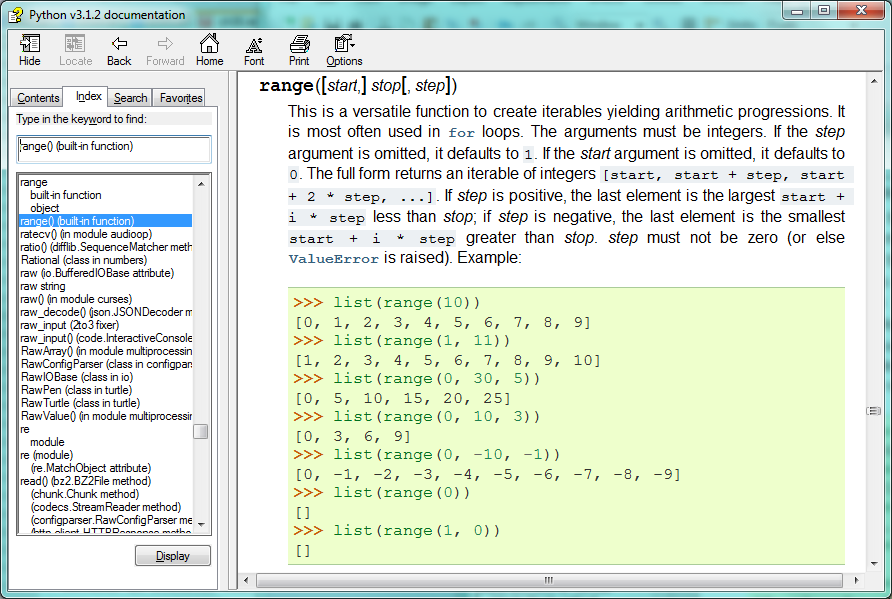
\includegraphics{help_range.png}

Notice the square brackets in the description of the arguments.
These are examples of \textbf{meta-notation} --- notation that describes
Python syntax, but is not part of it.
The square brackets in this documentation mean that the argument is
\emph{optional} --- the programmer can
omit it.  So what this first line of help tells us is that
\code{range} must always have a \code{stop} argument,
but it may have an optional \code{start} argument (which must be
followed by a comma if it is present),
and it can also have an optional \code{step} argument, preceded by
a comma if it is present.

The examples from help show that \code{range} can have either 1, 2 or 3 arguments.
The list can
start at any starting value, and go up or down in increments other than 1.
The documentation here also says that the arguments must be integers.

Other meta-notation you'll frequently encounter is the use of bold
and italics.  The bold means that these are tokens
--- keywords or symbols --- typed into your Python code exactly as
they are, whereas the italic terms stand for ``something of this type''.
So the syntax description
\begin{quote}

\textbf{for} \emph{variable} \textbf{in} \emph{list} \textbf{:}
\end{quote}

means you can substitute any legal
variable and any legal list when you write your Python code.

This (simplified) description of the \code{print} function, shows another example
of meta-notation in which the ellipses (\code{...}) mean that you can have as many
objects as you like (even zero), separated by commas:
\begin{quote}

\textbf{print( {[}}\emph{object,} ... \textbf{{]} )}
\end{quote}

Meta-notation gives us a concise and powerful way to describe the \emph{pattern} of some syntax
or feature.

\index{table}\index{logarithm}\index{Intel}\index{Pentium}\index{escape sequence}\index{tab}\index{newline}

\section{Tables}
\label{iteration:tables}\label{iteration:index-8}
One of the things loops are good for is generating tables.  Before
computers were readily available, people had to calculate logarithms, sines and
cosines, and other mathematical functions by hand. To make that easier,
mathematics books contained long tables listing the values of these functions.
Creating the tables was slow and boring, and they tended to be full of errors.

When computers appeared on the scene, one of the initial reactions was, \emph{``This is
great! We can use the computers to generate the tables, so there will be no
errors.''} That turned out to be true (mostly) but shortsighted. Soon thereafter,
computers and calculators were so pervasive that the tables became obsolete.

Well, almost. For some operations, computers use tables of values to get an
approximate answer and then perform computations to improve the approximation.
In some cases, there have been errors in the underlying tables, most famously
in the table the Intel Pentium processor chip used to perform floating-point division.

Although a log table is not as useful as it once was, it still makes a good
example of iteration. The following program outputs a sequence of values in the
left column and 2 raised to the power of that value in the right column:
\begin{quote}

\begin{Verbatim}[commandchars=\\\{\},numbers=left,firstnumber=1,stepnumber=1]
\PYG{k}{for} \PYG{n}{x} \PYG{o+ow}{in} \PYG{n+nb}{range}\PYG{p}{(}\PYG{l+m+mi}{13}\PYG{p}{)}\PYG{p}{:}   \PYG{c}{\PYGZsh{} Generate numbers 0 to 12}
    \PYG{n+nb}{print}\PYG{p}{(}\PYG{n}{x}\PYG{p}{,} \PYG{l+s}{"}\PYG{l+s+se}{\PYGZbs{}t}\PYG{l+s}{"}\PYG{p}{,} \PYG{l+m+mi}{2}\PYG{o}{*}\PYG{o}{*}\PYG{n}{x}\PYG{p}{)}
\end{Verbatim}
\end{quote}

The string \code{"\textbackslash{}t"} represents a \textbf{tab character}. The backslash character in
\code{"\textbackslash{}t"} indicates the beginning of an \textbf{escape sequence}.  Escape sequences
are used to represent invisible characters like tabs and newlines. The sequence
\code{\textbackslash{}n} represents a \textbf{newline}.

An escape sequence can appear anywhere in a string; in this example, the tab
escape sequence is the only thing in the string. How do you think you represent
a backslash in a string?

As characters and strings are displayed on the screen, an invisible marker
called the \textbf{cursor} keeps track of where the next character will go. After a
\code{print} function, the cursor normally goes to the beginning of the next
line.

The tab character shifts the cursor to the right until it reaches one of the
tab stops. Tabs are useful for making columns of text line up, as in the output
of the previous program:
\begin{quote}

\begin{Verbatim}[commandchars=\\\{\}]
\PYG{g+go}{0       1}
\PYG{g+go}{1       2}
\PYG{g+go}{2       4}
\PYG{g+go}{3       8}
\PYG{g+go}{4       16}
\PYG{g+go}{5       32}
\PYG{g+go}{6       64}
\PYG{g+go}{7       128}
\PYG{g+go}{8       256}
\PYG{g+go}{9       512}
\PYG{g+go}{10      1024}
\PYG{g+go}{11      2048}
\PYG{g+go}{12      4096}
\end{Verbatim}
\end{quote}

Because of the tab characters between the columns, the position of the second
column does not depend on the number of digits in the first column.

\index{two-dimensional table}

\section{Two-dimensional tables}
\label{iteration:index-9}\label{iteration:two-dimensional-tables}
A two-dimensional table is a table where you read the value at the intersection
of a row and a column. A multiplication table is a good example. Let's say you
want to print a multiplication table for the values from 1 to 6.

A good way to start is to write a loop that prints the multiples of 2, all on
one line:
\begin{quote}

\begin{Verbatim}[commandchars=\\\{\},numbers=left,firstnumber=1,stepnumber=1]
\PYG{k}{for} \PYG{n}{i} \PYG{o+ow}{in} \PYG{n+nb}{range}\PYG{p}{(}\PYG{l+m+mi}{1}\PYG{p}{,} \PYG{l+m+mi}{7}\PYG{p}{)}\PYG{p}{:}
    \PYG{n+nb}{print}\PYG{p}{(}\PYG{l+m+mi}{2} \PYG{o}{*} \PYG{n}{i}\PYG{p}{,} \PYG{n}{end}\PYG{o}{=}\PYG{l+s}{"}\PYG{l+s}{   }\PYG{l+s}{"}\PYG{p}{)}
\PYG{n+nb}{print}\PYG{p}{(}\PYG{p}{)}
\end{Verbatim}
\end{quote}

Here we've used the \code{range} function, but made it start its sequence at 1.
As the loop executes, the value of \code{i} changes from 1 to
6. When all the elements of the range have been assigned to \code{i}, the loop terminates.
Each time through the loop, it
displays the value of \code{2 * i}, followed by three spaces.

Again, the extra \code{end="   "} argument in the \code{print} function suppresses the newline, and
uses three spaces instead.  After the
loop completes, the call to \code{print} at line 3 finishes the current line, and starts a new line.

The output of the program is:
\begin{quote}

\begin{Verbatim}[commandchars=\\\{\}]
\PYG{g+go}{2      4      6      8      10     12}
\end{Verbatim}
\end{quote}

So far, so good. The next step is to \textbf{encapsulate} and \textbf{generalize}.

\index{encapsulation}\index{generalization}\index{program development}

\section{Encapsulation and generalization}
\label{iteration:encapsulation-and-generalization}\label{iteration:index-10}
Encapsulation is the process of wrapping a piece of code in a function,
allowing you to take advantage of all the things functions are good for. You
have already seen some examples of encapsulation, including \code{is\_divisible} in a previous chapter.

Generalization means taking something specific, such as printing the multiples
of 2, and making it more general, such as printing the multiples of any
integer.

This function encapsulates the previous loop and generalizes it to print
multiples of \code{n}:
\begin{quote}

\begin{Verbatim}[commandchars=\\\{\},numbers=left,firstnumber=1,stepnumber=1]
\PYG{k}{def} \PYG{n+nf}{print\PYGZus{}multiples}\PYG{p}{(}\PYG{n}{n}\PYG{p}{)}\PYG{p}{:}
    \PYG{k}{for} \PYG{n}{i} \PYG{o+ow}{in} \PYG{n+nb}{range}\PYG{p}{(}\PYG{l+m+mi}{1}\PYG{p}{,} \PYG{l+m+mi}{7}\PYG{p}{)}\PYG{p}{:}
        \PYG{n+nb}{print}\PYG{p}{(}\PYG{n}{n} \PYG{o}{*} \PYG{n}{i}\PYG{p}{,} \PYG{n}{end}\PYG{o}{=}\PYG{l+s}{"}\PYG{l+s}{   }\PYG{l+s}{"}\PYG{p}{)}
    \PYG{n+nb}{print}\PYG{p}{(}\PYG{p}{)}
\end{Verbatim}
\end{quote}

To encapsulate, all we had to do was add the first line, which declares the
name of the function and the parameter list. To generalize, all we had to do
was replace the value 2 with the parameter \code{n}.

If we call this function with the argument 2, we get the same output as before.
With the argument 3, the output is:
\begin{quote}

\begin{Verbatim}[commandchars=\\\{\}]
\PYG{g+go}{3      6      9      12     15     18}
\end{Verbatim}
\end{quote}

With the argument 4, the output is:
\begin{quote}

\begin{Verbatim}[commandchars=\\\{\}]
\PYG{g+go}{4      8      12     16     20     24}
\end{Verbatim}
\end{quote}

By now you can probably guess how to print a multiplication table --- by
calling \code{print\_multiples} repeatedly with different arguments. In fact, we
can use another loop:
\begin{quote}

\begin{Verbatim}[commandchars=\\\{\},numbers=left,firstnumber=1,stepnumber=1]
\PYG{k}{for} \PYG{n}{i} \PYG{o+ow}{in} \PYG{n+nb}{range}\PYG{p}{(}\PYG{l+m+mi}{1}\PYG{p}{,} \PYG{l+m+mi}{7}\PYG{p}{)}\PYG{p}{:}
    \PYG{n}{print\PYGZus{}multiples}\PYG{p}{(}\PYG{n}{i}\PYG{p}{)}
\end{Verbatim}
\end{quote}

Notice how similar this loop is to the one inside \code{print\_multiples}.  All we
did was replace the \code{print} function with a function call.

The output of this program is a multiplication table:
\begin{quote}

\begin{Verbatim}[commandchars=\\\{\}]
\PYG{g+go}{1      2      3      4      5      6}
\PYG{g+go}{2      4      6      8      10     12}
\PYG{g+go}{3      6      9      12     15     18}
\PYG{g+go}{4      8      12     16     20     24}
\PYG{g+go}{5      10     15     20     25     30}
\PYG{g+go}{6      12     18     24     30     36}
\end{Verbatim}
\end{quote}

\index{development plan}

\section{More encapsulation}
\label{iteration:more-encapsulation}\label{iteration:index-11}
To demonstrate encapsulation again, let's take the code from the last section
and wrap it up in a function:
\begin{quote}

\begin{Verbatim}[commandchars=\\\{\},numbers=left,firstnumber=1,stepnumber=1]
\PYG{k}{def} \PYG{n+nf}{print\PYGZus{}mult\PYGZus{}table}\PYG{p}{(}\PYG{p}{)}\PYG{p}{:}
    \PYG{k}{for} \PYG{n}{i} \PYG{o+ow}{in} \PYG{n+nb}{range}\PYG{p}{(}\PYG{l+m+mi}{1}\PYG{p}{,} \PYG{l+m+mi}{7}\PYG{p}{)}\PYG{p}{:}
        \PYG{n}{print\PYGZus{}multiples}\PYG{p}{(}\PYG{n}{i}\PYG{p}{)}
\end{Verbatim}
\end{quote}

This process is a common \textbf{development plan}. We develop code by writing lines
of code outside any function, or typing them in to the interpreter. When we get
the code working, we extract it and wrap it up in a function.

This development plan is particularly useful if you don't know how to divide
the program into functions when you start writing. This approach lets you
design as you go along.

\index{local variable}\index{variable!local}

\section{Local variables}
\label{iteration:local-variables}\label{iteration:index-12}
You might be wondering how we can use the same variable, \code{i}, in both
\code{print\_multiples} and \code{print\_mult\_table}. Doesn't it cause problems when
one of the functions changes the value of the variable?

The answer is no, because the \code{i} in \code{print\_multiples} and the \code{i} in
\code{print\_mult\_table} are \emph{not} the same variable.

Variables created inside a function definition are local; you can't access a
local variable from outside its home function. That means you are free to have
multiple variables with the same name as long as they are not in the same
function.

Python examines all the statements in a function --- if any of them assign a value
to a variable, that is the clue that Python uses to make the variable a local variable.

The stack diagram for this program shows that the two variables named \code{i} are
not the same variable. They can refer to different values, and changing one
does not affect the other.
\begin{quote}

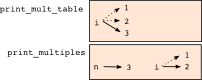
\includegraphics{stack2.png}
\end{quote}

The value of \code{i} in \code{print\_mult\_table} goes from 1 to 6. In the diagram it
happens to be 3. The next time through the loop it will be 4. Each time through
the loop, \code{print\_mult\_table} calls \code{print\_multiples} with the current value
of \code{i} as an argument. That value gets assigned to the parameter \code{n}.

Inside \code{print\_multiples}, the value of \code{i} goes from 1 to 6. In the
diagram, it happens to be 2. Changing this variable has no effect on the value
of \code{i} in \code{print\_mult\_table}.

It is common and perfectly legal to have different local variables with the
same name. In particular, names like \code{i} and \code{j} are used frequently as
loop variables. If you avoid using them in one function just because you used
them somewhere else, you will probably make the program harder to read.

The visualizer at \href{http://netserv.ict.ru.ac.za/python3\_viz/}{http://netserv.ict.ru.ac.za/python3\_viz/} shows very clearly how the
two variables \code{i} are distinct variables, and how they have independent values.

\index{break statement}\index{statement: break}

\section{The \texttt{break} statement}
\label{iteration:the-break-statement}\label{iteration:index-13}
The \textbf{break} statement is used to immediately leave the body of its loop.  The next
statement to be executed is the first one after the body:
\begin{quote}

\begin{Verbatim}[commandchars=\\\{\},numbers=left,firstnumber=1,stepnumber=1]
\PYG{k}{for} \PYG{n}{i} \PYG{o+ow}{in} \PYG{p}{[}\PYG{l+m+mi}{12}\PYG{p}{,} \PYG{l+m+mi}{16}\PYG{p}{,} \PYG{l+m+mi}{17}\PYG{p}{,} \PYG{l+m+mi}{24}\PYG{p}{,} \PYG{l+m+mi}{29}\PYG{p}{]}\PYG{p}{:}
    \PYG{k}{if} \PYG{n}{i} \PYG{o}{\PYGZpc{}} \PYG{l+m+mi}{2} \PYG{o}{==} \PYG{l+m+mi}{1}\PYG{p}{:}  \PYG{c}{\PYGZsh{} If the number is odd}
       \PYG{k}{break}        \PYG{c}{\PYGZsh{}  ... immediately exit the loop}
    \PYG{n+nb}{print}\PYG{p}{(}\PYG{n}{i}\PYG{p}{)}
\PYG{n+nb}{print}\PYG{p}{(}\PYG{l+s}{"}\PYG{l+s}{done}\PYG{l+s}{"}\PYG{p}{)}
\end{Verbatim}
\end{quote}

This prints:
\begin{quote}

\begin{Verbatim}[commandchars=\\\{\}]
\PYG{g+go}{12}
\PYG{g+go}{16}
\PYG{g+go}{done}
\end{Verbatim}
\end{quote}

\begin{notice}{note}{The pre-test loop --- standard loop behaviour}

\code{for} and \code{while} loops do their tests at the start, before executing
any part of the body.   They're called \textbf{pre-test} loops, because the test
happens before (pre) the body.
\code{break} and \code{return} are our tools for adapting this standard behaviour.

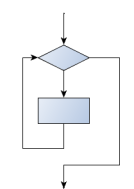
\includegraphics{pre_test_loop.png}
\end{notice}


\section{Other flavours of loops}
\label{iteration:other-flavours-of-loops}
Sometimes we'd like to have the \textbf{middle-test} loop with the exit test in the middle
of the body, rather than at the beginning or at the end.  Or a \textbf{post-test} loop that
puts its exit test as the last thing in the body. Other languages have different
syntax and keywords for these different flavours, but Python just uses
a combination of \code{while} and \code{if condition: break} to get the job done.

A typical example is a problem where the user has to input numbers to be summed.
To indicate that there are no more inputs, the user enters a special value, often
the value -1, or the empty string.  This needs a middle-exit loop pattern:
input the next number, then test whether to exit, or else process the number:
\begin{quote}

\begin{notice}{note}{The middle-test loop flowchart}

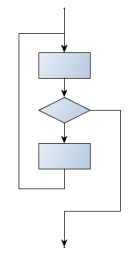
\includegraphics{mid_test_loop.png}
\end{notice}

\begin{Verbatim}[commandchars=\\\{\},numbers=left,firstnumber=1,stepnumber=1]
\PYG{n}{total} \PYG{o}{=} \PYG{l+m+mi}{0}
\PYG{k}{while} \PYG{k}{True}\PYG{p}{:}
    \PYG{n}{response} \PYG{o}{=} \PYG{n+nb}{input}\PYG{p}{(}\PYG{l+s}{"}\PYG{l+s}{Enter the next number. (Leave blank to end)}\PYG{l+s}{"}\PYG{p}{)}
    \PYG{k}{if} \PYG{n}{response} \PYG{o}{==} \PYG{l+s}{"}\PYG{l+s}{"}\PYG{p}{:}
        \PYG{k}{break}
    \PYG{n}{total} \PYG{o}{+}\PYG{o}{=} \PYG{n+nb}{int}\PYG{p}{(}\PYG{n}{response}\PYG{p}{)}
\PYG{n+nb}{print}\PYG{p}{(}\PYG{l+s}{"}\PYG{l+s}{The total of the numbers you entered is }\PYG{l+s}{"}\PYG{p}{,} \PYG{n}{total}\PYG{p}{)}
\end{Verbatim}
\end{quote}

Convince yourself that this fits the middle-exit loop flowchart: line 3
does some useful work, lines 4 and 5 can exit the loop, and if they don't
line 6 does more useful work before the next iteration starts.

The \code{while bool-expr:} uses the Boolean expression to determine whether to iterate again.
\code{True} is a trivial Boolean expression, so \code{while True:}  means \emph{always do
the loop body again}.  This is a language \emph{idiom} --- a convention that
most programmers will recognize immediately. Since the expression on line 2
will never terminate the loop, (it is a dummy test) the programmer must arrange to
break (or return) out of the loop body elsewhere, in some other way (i.e. in lines 4 and 5 in
this sample). A clever compiler or interpreter will understand that line 2 is a
fake test that must always succeed, so it won't even generate a test, and our flowchart
never even put the diamond-shape dummy test box at the top of the loop!

Similarly, by just moving the \code{if condition: break} to the end of the loop body we
create a pattern for a post-test loop.  Post-test loops are used when you want to
be sure that the loop body always executes at least once (because the first test
only happens at the end of the execution of the first loop body).
This is useful, for example, if we want to play an interactive game against
the user --- we always want to play at least one game:
\begin{quote}

\begin{Verbatim}[commandchars=\\\{\},numbers=left,firstnumber=1,stepnumber=1]
\PYG{k}{while} \PYG{k}{True}\PYG{p}{:}
    \PYG{n}{play\PYGZus{}the\PYGZus{}game\PYGZus{}once}\PYG{p}{(}\PYG{p}{)}
    \PYG{n}{response} \PYG{o}{=} \PYG{n+nb}{input}\PYG{p}{(}\PYG{l+s}{"}\PYG{l+s}{Play again? (yes or no)}\PYG{l+s}{"}\PYG{p}{)}
    \PYG{k}{if} \PYG{n}{response} \PYG{o}{!=} \PYG{l+s}{"}\PYG{l+s}{yes}\PYG{l+s}{"}\PYG{p}{:}
        \PYG{k}{break}
\PYG{n+nb}{print}\PYG{p}{(}\PYG{l+s}{"}\PYG{l+s}{Goodbye!}\PYG{l+s}{"}\PYG{p}{)}
\end{Verbatim}
\end{quote}

\begin{notice}{note}{Hint: Think about where you want the exit test to happen}

Once you've recognized that you need a loop to repeat something, think
about its terminating condition --- when will I want to stop iterating?
Then figure out whether you need to do the test before starting
the first (and every other) iteration, or at the end of
the first (and every other) iteration, or perhaps in
the middle of each iteration.  Interactive programs that require input
from the user or read from files often need to exit their loops in the
middle or at the end of an iteration, when it becomes clear that there is
no more data to process, or the user doesn't want to play our game anymore.
\end{notice}


\section{An example}
\label{iteration:an-example}
The following program implements a simple guessing game:
\begin{quote}

\begin{Verbatim}[commandchars=\\\{\},numbers=left,firstnumber=1,stepnumber=1]
\PYG{k+kn}{import} \PYG{n+nn}{random}                   \PYG{c}{\PYGZsh{} We cover random numbers in the}
\PYG{n}{rng} \PYG{o}{=} \PYG{n}{random}\PYG{o}{.}\PYG{n}{Random}\PYG{p}{(}\PYG{p}{)}           \PYG{c}{\PYGZsh{}  modules chapter, so peek ahead.}
\PYG{n}{number} \PYG{o}{=} \PYG{n}{rng}\PYG{o}{.}\PYG{n}{randrange}\PYG{p}{(}\PYG{l+m+mi}{1}\PYG{p}{,} \PYG{l+m+mi}{1000}\PYG{p}{)} \PYG{c}{\PYGZsh{} Get random number between [1 and 1000).}

\PYG{n}{guesses} \PYG{o}{=} \PYG{l+m+mi}{0}
\PYG{n}{msg} \PYG{o}{=} \PYG{l+s}{"}\PYG{l+s}{"}

\PYG{k}{while} \PYG{k}{True}\PYG{p}{:}
    \PYG{n}{guess} \PYG{o}{=} \PYG{n+nb}{int}\PYG{p}{(}\PYG{n+nb}{input}\PYG{p}{(}\PYG{n}{msg} \PYG{o}{+} \PYG{l+s}{"}\PYG{l+s+se}{\PYGZbs{}n}\PYG{l+s}{Guess my number between 1 and 1000: }\PYG{l+s}{"}\PYG{p}{)}\PYG{p}{)}
    \PYG{n}{guesses} \PYG{o}{+}\PYG{o}{=} \PYG{l+m+mi}{1}
    \PYG{k}{if} \PYG{n}{guess} \PYG{o}{\PYGZgt{}} \PYG{n}{number}\PYG{p}{:}
        \PYG{n}{msg} \PYG{o}{+}\PYG{o}{=} \PYG{n+nb}{str}\PYG{p}{(}\PYG{n}{guess}\PYG{p}{)} \PYG{o}{+} \PYG{l+s}{"}\PYG{l+s}{ is too high.}\PYG{l+s+se}{\PYGZbs{}n}\PYG{l+s}{"}
    \PYG{k}{elif} \PYG{n}{guess} \PYG{o}{\PYGZlt{}} \PYG{n}{number}\PYG{p}{:}
        \PYG{n}{msg} \PYG{o}{+}\PYG{o}{=} \PYG{n+nb}{str}\PYG{p}{(}\PYG{n}{guess}\PYG{p}{)} \PYG{o}{+} \PYG{l+s}{"}\PYG{l+s}{ is too low.}\PYG{l+s+se}{\PYGZbs{}n}\PYG{l+s}{"}
    \PYG{k}{else}\PYG{p}{:}
        \PYG{k}{break}

\PYG{n+nb}{input}\PYG{p}{(}\PYG{l+s}{"}\PYG{l+s+se}{\PYGZbs{}n}\PYG{l+s+se}{\PYGZbs{}n}\PYG{l+s}{Great, you got it in \PYGZob{}0\PYGZcb{} guesses!}\PYG{l+s+se}{\PYGZbs{}n}\PYG{l+s+se}{\PYGZbs{}n}\PYG{l+s}{"}\PYG{o}{.}\PYG{n}{format}\PYG{p}{(}\PYG{n}{guesses}\PYG{p}{)}\PYG{p}{)}
\end{Verbatim}
\end{quote}

This program makes use of the mathematical law of \textbf{trichotomy} (given real
numbers a and b, exactly one of these three must be true:  a \textgreater{} b, a \textless{} b, or a == b).

At line 18 there is a call to the input function, but we don't do
anything with the result, not even assign it to a variable.  This is legal in Python.
Here it has the effect of popping up the input dialog window and waiting for the
user to respond before the program terminates.  Programmers often use the trick
of doing some extra input at the end of a script, just to keep the window open.

Also notice the use of the \code{msg} variable, initially an empty string, on lines 6, 12 and 14.
Each time through the loop we extend the message being displayed: this allows us to
display the program's feedback right at the same place as we're asking for the next guess.
\begin{quote}

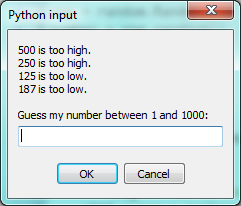
\includegraphics{python_input.png}
\end{quote}

\index{continue statement}\index{statement!continue}

\section{The \texttt{continue} statement}
\label{iteration:index-14}\label{iteration:the-continue-statement}
This is a control flow statement that causes the program to immediately skip the
processing of the rest of the body of the loop, \emph{for the current iteration}.  But
the loop still carries on running for its remaining iterations:
\begin{quote}

\begin{Verbatim}[commandchars=\\\{\},numbers=left,firstnumber=1,stepnumber=1]
\PYG{k}{for} \PYG{n}{i} \PYG{o+ow}{in} \PYG{p}{[}\PYG{l+m+mi}{12}\PYG{p}{,} \PYG{l+m+mi}{16}\PYG{p}{,} \PYG{l+m+mi}{17}\PYG{p}{,} \PYG{l+m+mi}{24}\PYG{p}{,} \PYG{l+m+mi}{29}\PYG{p}{,} \PYG{l+m+mi}{30}\PYG{p}{]}\PYG{p}{:}
    \PYG{k}{if} \PYG{n}{i} \PYG{o}{\PYGZpc{}} \PYG{l+m+mi}{2} \PYG{o}{==} \PYG{l+m+mi}{1}\PYG{p}{:}      \PYG{c}{\PYGZsh{} If the number is odd}
       \PYG{k}{continue}         \PYG{c}{\PYGZsh{} Don't process it}
    \PYG{n+nb}{print}\PYG{p}{(}\PYG{n}{i}\PYG{p}{)}
\PYG{n+nb}{print}\PYG{p}{(}\PYG{l+s}{"}\PYG{l+s}{done}\PYG{l+s}{"}\PYG{p}{)}
\end{Verbatim}
\end{quote}

This prints:
\begin{quote}

\begin{Verbatim}[commandchars=\\\{\}]
\PYG{g+go}{12}
\PYG{g+go}{16}
\PYG{g+go}{24}
\PYG{g+go}{30}
\PYG{g+go}{done}
\end{Verbatim}
\end{quote}


\section{More generalization}
\label{iteration:more-generalization}
As another example of generalization, imagine you wanted a program that would
print a multiplication table of any size, not just the six-by-six table. You
could add a parameter to \code{print\_mult\_table}:
\begin{quote}

\begin{Verbatim}[commandchars=\\\{\},numbers=left,firstnumber=1,stepnumber=1]
\PYG{k}{def} \PYG{n+nf}{print\PYGZus{}mult\PYGZus{}table}\PYG{p}{(}\PYG{n}{high}\PYG{p}{)}\PYG{p}{:}
    \PYG{k}{for} \PYG{n}{i} \PYG{o+ow}{in} \PYG{n+nb}{range}\PYG{p}{(}\PYG{l+m+mi}{1}\PYG{p}{,} \PYG{n}{high}\PYG{o}{+}\PYG{l+m+mi}{1}\PYG{p}{)}\PYG{p}{:}
        \PYG{n}{print\PYGZus{}multiples}\PYG{p}{(}\PYG{n}{i}\PYG{p}{)}
\end{Verbatim}
\end{quote}

We replaced the value 7 with the expression \code{high+1}. If we call
\code{print\_mult\_table} with the argument 7, it displays:
\begin{quote}

\begin{Verbatim}[commandchars=\\\{\}]
\PYG{g+go}{1      2      3      4      5      6}
\PYG{g+go}{2      4      6      8      10     12}
\PYG{g+go}{3      6      9      12     15     18}
\PYG{g+go}{4      8      12     16     20     24}
\PYG{g+go}{5      10     15     20     25     30}
\PYG{g+go}{6      12     18     24     30     36}
\PYG{g+go}{7      14     21     28     35     42}
\end{Verbatim}
\end{quote}

This is fine, except that we probably want the table to be square --- with the
same number of rows and columns. To do that, we add another parameter to
\code{print\_multiples} to specify how many columns the table should have.

Just to be annoying, we call this parameter \code{high}, demonstrating that
different functions can have parameters with the same name (just like local
variables). Here's the whole program:
\begin{quote}

\begin{Verbatim}[commandchars=\\\{\},numbers=left,firstnumber=1,stepnumber=1]
\PYG{k}{def} \PYG{n+nf}{print\PYGZus{}multiples}\PYG{p}{(}\PYG{n}{n}\PYG{p}{,} \PYG{n}{high}\PYG{p}{)}\PYG{p}{:}
    \PYG{k}{for} \PYG{n}{i} \PYG{o+ow}{in} \PYG{n+nb}{range}\PYG{p}{(}\PYG{l+m+mi}{1}\PYG{p}{,} \PYG{n}{high}\PYG{o}{+}\PYG{l+m+mi}{1}\PYG{p}{)}\PYG{p}{:}
        \PYG{n+nb}{print}\PYG{p}{(}\PYG{n}{n} \PYG{o}{*} \PYG{n}{i}\PYG{p}{,} \PYG{n}{end}\PYG{o}{=}\PYG{l+s}{"}\PYG{l+s}{   }\PYG{l+s}{"}\PYG{p}{)}
    \PYG{n+nb}{print}\PYG{p}{(}\PYG{p}{)}

\PYG{k}{def} \PYG{n+nf}{print\PYGZus{}mult\PYGZus{}table}\PYG{p}{(}\PYG{n}{high}\PYG{p}{)}\PYG{p}{:}
    \PYG{k}{for} \PYG{n}{i} \PYG{o+ow}{in} \PYG{n+nb}{range}\PYG{p}{(}\PYG{l+m+mi}{1}\PYG{p}{,} \PYG{n}{high}\PYG{o}{+}\PYG{l+m+mi}{1}\PYG{p}{)}\PYG{p}{:}
        \PYG{n}{print\PYGZus{}multiples}\PYG{p}{(}\PYG{n}{i}\PYG{p}{,} \PYG{n}{high}\PYG{p}{)}
\end{Verbatim}
\end{quote}

Notice that when we added a new parameter, we had to change the first line of
the function (the function heading), and we also had to change the place where
the function is called in \code{print\_mult\_table}.

Now, when we call \code{print\_mult\_table(7)}:
\begin{quote}

\begin{Verbatim}[commandchars=\\\{\}]
\PYG{g+go}{1      2      3      4      5      6      7}
\PYG{g+go}{2      4      6      8      10     12     14}
\PYG{g+go}{3      6      9      12     15     18     21}
\PYG{g+go}{4      8      12     16     20     24     28}
\PYG{g+go}{5      10     15     20     25     30     35}
\PYG{g+go}{6      12     18     24     30     36     42}
\PYG{g+go}{7      14     21     28     35     42     49}
\end{Verbatim}
\end{quote}

When you generalize a function appropriately, you often get a program with
capabilities you didn't plan. For example, you might notice that, because ab =
ba, all the entries in the table appear twice. You could save ink by printing
only half the table. To do that, you only have to change one line of
\code{print\_mult\_table}. Change
\begin{quote}

\begin{Verbatim}[commandchars=\\\{\},numbers=left,firstnumber=1,stepnumber=1]
\PYG{n}{print\PYGZus{}multiples}\PYG{p}{(}\PYG{n}{i}\PYG{p}{,} \PYG{n}{high}\PYG{o}{+}\PYG{l+m+mi}{1}\PYG{p}{)}
\end{Verbatim}
\end{quote}

to
\begin{quote}

\begin{Verbatim}[commandchars=\\\{\},numbers=left,firstnumber=1,stepnumber=1]
\PYG{n}{print\PYGZus{}multiples}\PYG{p}{(}\PYG{n}{i}\PYG{p}{,} \PYG{n}{i}\PYG{o}{+}\PYG{l+m+mi}{1}\PYG{p}{)}
\end{Verbatim}
\end{quote}

and you get:

\begin{Verbatim}[commandchars=\\\{\}]
1
2      4
3      6      9
4      8      12     16
5      10     15     20     25
6      12     18     24     30     36
7      14     21     28     35     42     49
\end{Verbatim}

\index{function}

\section{Functions}
\label{iteration:functions}\label{iteration:index-15}
A few times now, we have mentioned all the things functions are good for. By
now, you might be wondering what exactly those things are.  Here are some of
them:
\begin{enumerate}
\item {} 
Capturing your mental chunking. Breaking your complex tasks into sub-tasks, and
giving the sub-tasks a meaningful name is a powerful mental technique.  Look back
at the example that illustrated the post-test loop: we assumed that we had a function
called \code{play\_the\_game\_once}.  This chunking allowed us to put aside the details
of the particular game --- is it a card game, or noughts and crosses, or a role playing
game --- and simply focus on one isolated part of our program logic --- letting the player
choose whether they want to play again.

\item {} 
Dividing a long program into functions allows you to separate parts of the
program, debug them in isolation, and then compose them into a whole.

\item {} 
Functions facilitate the use of iteration.

\item {} 
Well-designed functions are often useful for many programs. Once you write
and debug one, you can reuse it.

\end{enumerate}


\section{Paired Data}
\label{iteration:paired-data}
We've already seen lists of names and lists of numbers in Python. We're going to peek ahead in
the textbook a little, and show a more advanced way of representing our data.
Making a pair of things in Python is as simple as putting them into parentheses,
like this:
\begin{quote}

\begin{Verbatim}[commandchars=\\\{\},numbers=left,firstnumber=1,stepnumber=1]
\PYG{n}{year\PYGZus{}born} \PYG{o}{=} \PYG{p}{(}\PYG{l+s}{"}\PYG{l+s}{Paris Hilton}\PYG{l+s}{"}\PYG{p}{,} \PYG{l+m+mi}{1981}\PYG{p}{)}
\end{Verbatim}
\end{quote}

We can put many pairs into a list of pairs:
\begin{quote}

\begin{Verbatim}[commandchars=\\\{\},numbers=left,firstnumber=1,stepnumber=1]
\PYG{n}{celebs} \PYG{o}{=} \PYG{p}{[}\PYG{p}{(}\PYG{l+s}{"}\PYG{l+s}{Brad Pitt}\PYG{l+s}{"}\PYG{p}{,} \PYG{l+m+mi}{1963}\PYG{p}{)}\PYG{p}{,} \PYG{p}{(}\PYG{l+s}{"}\PYG{l+s}{Jack Nicholson}\PYG{l+s}{"}\PYG{p}{,} \PYG{l+m+mi}{1937}\PYG{p}{)}\PYG{p}{,}
                                \PYG{p}{(}\PYG{l+s}{"}\PYG{l+s}{Justin Bieber}\PYG{l+s}{"}\PYG{p}{,} \PYG{l+m+mi}{1994}\PYG{p}{)}\PYG{p}{]}
\end{Verbatim}
\end{quote}

Here is a quick sample of things we can do with structured data like this.  First,
print all the celebs:
\begin{quote}

\begin{Verbatim}[commandchars=\\\{\},numbers=left,firstnumber=1,stepnumber=1]
\PYG{n+nb}{print}\PYG{p}{(}\PYG{n}{celebs}\PYG{p}{)}
\PYG{n+nb}{print}\PYG{p}{(}\PYG{n+nb}{len}\PYG{p}{(}\PYG{n}{celebs}\PYG{p}{)}\PYG{p}{)}
\end{Verbatim}

\begin{Verbatim}[commandchars=\\\{\}]
\PYG{g+go}{[("Brad Pitt", 1963), ("Jack Nicholson", 1937), ("Justin Bieber", 1994)]}
\PYG{g+go}{3}
\end{Verbatim}
\end{quote}

Notice that the \code{celebs} list has just 3 elements, each of them pairs.

Now we print the names of those celebrities born before 1980:
\begin{quote}

\begin{Verbatim}[commandchars=\\\{\},numbers=left,firstnumber=1,stepnumber=1]
\PYG{k}{for} \PYG{p}{(}\PYG{n}{nm}\PYG{p}{,} \PYG{n}{yr}\PYG{p}{)} \PYG{o+ow}{in} \PYG{n}{celebs}\PYG{p}{:}
   \PYG{k}{if} \PYG{n}{yr} \PYG{o}{\PYGZlt{}} \PYG{l+m+mi}{1980}\PYG{p}{:}
        \PYG{n+nb}{print}\PYG{p}{(}\PYG{n}{nm}\PYG{p}{)}
\end{Verbatim}

\begin{Verbatim}[commandchars=\\\{\}]
\PYG{g+go}{Brad Pitt}
\PYG{g+go}{Jack Nicholson}
\end{Verbatim}
\end{quote}

This demonstrates something we have not seen yet in the \code{for} loop: instead of using a single
loop control variable, we've used a pair of variable names, \code{(nm, yr)},  instead.
The loop is executed three times --- once for each pair in the list, and on each iteration both the
variables are assigned values from the pair of data that is being handled.


\section{Nested Loops for Nested Data}
\label{iteration:nested-loops-for-nested-data}\label{iteration:nested-data}
Now we'll come up with an even more adventurous list of structured data.  In this case,
we have a list of students.  Each student has a name which is paired up with another list
of subjects that they are enrolled for:
\begin{quote}

\begin{Verbatim}[commandchars=\\\{\},numbers=left,firstnumber=1,stepnumber=1]
\PYG{n}{students} \PYG{o}{=} \PYG{p}{[}
    \PYG{p}{(}\PYG{l+s}{"}\PYG{l+s}{John}\PYG{l+s}{"}\PYG{p}{,} \PYG{p}{[}\PYG{l+s}{"}\PYG{l+s}{CompSci}\PYG{l+s}{"}\PYG{p}{,} \PYG{l+s}{"}\PYG{l+s}{Physics}\PYG{l+s}{"}\PYG{p}{]}\PYG{p}{)}\PYG{p}{,}
    \PYG{p}{(}\PYG{l+s}{"}\PYG{l+s}{Vusi}\PYG{l+s}{"}\PYG{p}{,} \PYG{p}{[}\PYG{l+s}{"}\PYG{l+s}{Maths}\PYG{l+s}{"}\PYG{p}{,} \PYG{l+s}{"}\PYG{l+s}{CompSci}\PYG{l+s}{"}\PYG{p}{,} \PYG{l+s}{"}\PYG{l+s}{Stats}\PYG{l+s}{"}\PYG{p}{]}\PYG{p}{)}\PYG{p}{,}
    \PYG{p}{(}\PYG{l+s}{"}\PYG{l+s}{Jess}\PYG{l+s}{"}\PYG{p}{,} \PYG{p}{[}\PYG{l+s}{"}\PYG{l+s}{CompSci}\PYG{l+s}{"}\PYG{p}{,} \PYG{l+s}{"}\PYG{l+s}{Accounting}\PYG{l+s}{"}\PYG{p}{,} \PYG{l+s}{"}\PYG{l+s}{Economics}\PYG{l+s}{"}\PYG{p}{,} \PYG{l+s}{"}\PYG{l+s}{Management}\PYG{l+s}{"}\PYG{p}{]}\PYG{p}{)}\PYG{p}{,}
    \PYG{p}{(}\PYG{l+s}{"}\PYG{l+s}{Sarah}\PYG{l+s}{"}\PYG{p}{,} \PYG{p}{[}\PYG{l+s}{"}\PYG{l+s}{InfSys}\PYG{l+s}{"}\PYG{p}{,} \PYG{l+s}{"}\PYG{l+s}{Accounting}\PYG{l+s}{"}\PYG{p}{,} \PYG{l+s}{"}\PYG{l+s}{Economics}\PYG{l+s}{"}\PYG{p}{,} \PYG{l+s}{"}\PYG{l+s}{CommLaw}\PYG{l+s}{"}\PYG{p}{]}\PYG{p}{)}\PYG{p}{,}
    \PYG{p}{(}\PYG{l+s}{"}\PYG{l+s}{Zuki}\PYG{l+s}{"}\PYG{p}{,} \PYG{p}{[}\PYG{l+s}{"}\PYG{l+s}{Sociology}\PYG{l+s}{"}\PYG{p}{,} \PYG{l+s}{"}\PYG{l+s}{Economics}\PYG{l+s}{"}\PYG{p}{,} \PYG{l+s}{"}\PYG{l+s}{Law}\PYG{l+s}{"}\PYG{p}{,} \PYG{l+s}{"}\PYG{l+s}{Stats}\PYG{l+s}{"}\PYG{p}{,} \PYG{l+s}{"}\PYG{l+s}{Music}\PYG{l+s}{"}\PYG{p}{]}\PYG{p}{)}\PYG{p}{]}
\end{Verbatim}
\end{quote}

Here we've assigned a list of five elements to the variable \code{students}.  Let's print
out each student name, and the number of subjects they are enrolled for:
\begin{quote}

\begin{Verbatim}[commandchars=\\\{\},numbers=left,firstnumber=1,stepnumber=1]
\PYG{c}{\PYGZsh{} Print all students with a count of their courses.}
\PYG{k}{for} \PYG{p}{(}\PYG{n}{name}\PYG{p}{,} \PYG{n}{subjects}\PYG{p}{)} \PYG{o+ow}{in} \PYG{n}{students}\PYG{p}{:}
    \PYG{n+nb}{print}\PYG{p}{(}\PYG{n}{name}\PYG{p}{,} \PYG{l+s}{"}\PYG{l+s}{takes}\PYG{l+s}{"}\PYG{p}{,} \PYG{n+nb}{len}\PYG{p}{(}\PYG{n}{subjects}\PYG{p}{)}\PYG{p}{,} \PYG{l+s}{"}\PYG{l+s}{courses}\PYG{l+s}{"}\PYG{p}{)}
\end{Verbatim}
\end{quote}

Python agreeably responds with the following output:
\begin{quote}

\begin{Verbatim}[commandchars=\\\{\}]
\PYG{g+go}{John takes 2 courses}
\PYG{g+go}{Vusi takes 3 courses}
\PYG{g+go}{Jess takes 4 courses}
\PYG{g+go}{Sarah takes 4 courses}
\PYG{g+go}{Zuki takes 5 courses}
\end{Verbatim}
\end{quote}

Now we'd like to ask how many students are taking CompSci. This needs a counter,
and for each student we need a second loop that tests each of the subjects in turn:
\begin{quote}

\begin{Verbatim}[commandchars=\\\{\},numbers=left,firstnumber=1,stepnumber=1]
\PYG{c}{\PYGZsh{} Count how many students are taking CompSci}
\PYG{n}{counter} \PYG{o}{=} \PYG{l+m+mi}{0}
\PYG{k}{for} \PYG{p}{(}\PYG{n}{name}\PYG{p}{,} \PYG{n}{subjects}\PYG{p}{)} \PYG{o+ow}{in} \PYG{n}{students}\PYG{p}{:}
    \PYG{k}{for} \PYG{n}{s} \PYG{o+ow}{in} \PYG{n}{subjects}\PYG{p}{:}                 \PYG{c}{\PYGZsh{} A nested loop!}
        \PYG{k}{if} \PYG{n}{s} \PYG{o}{==} \PYG{l+s}{"}\PYG{l+s}{CompSci}\PYG{l+s}{"}\PYG{p}{:}
           \PYG{n}{counter} \PYG{o}{+}\PYG{o}{=} \PYG{l+m+mi}{1}

\PYG{n+nb}{print}\PYG{p}{(}\PYG{l+s}{"}\PYG{l+s}{The number of students taking CompSci is}\PYG{l+s}{"}\PYG{p}{,} \PYG{n}{counter}\PYG{p}{)}
\end{Verbatim}

\begin{Verbatim}[commandchars=\\\{\}]
\PYG{g+go}{The number of students taking CompSci is 3}
\end{Verbatim}
\end{quote}

You should set up a list of your own data that interests you  ---
perhaps a list of your CDs, each containing a list of song titles on the CD,
or a list of movie titles, each with a list of movie stars who acted in the movie.
You could then ask questions like ``Which movies starred Angelina Jolie?''

\index{Newton's method}

\section{Newton's method for finding square roots}
\label{iteration:index-16}\label{iteration:newton-s-method-for-finding-square-roots}
Loops are often used in programs that compute numerical results by starting
with an approximate answer and iteratively improving it.

For example, before we had calculators or computers, people needed to
calculate square roots manually.  Newton used a particularly good
method (there is some evidence that this method was known many years before).
Suppose that you want to know the square root of \code{n}. If you start
with almost any approximation, you can compute a better approximation (closer
to the actual answer) with the following formula:
\begin{quote}

\begin{Verbatim}[commandchars=\\\{\},numbers=left,firstnumber=1,stepnumber=1]
\PYG{n}{better} \PYG{o}{=} \PYG{p}{(}\PYG{n}{approx} \PYG{o}{+} \PYG{n}{n}\PYG{o}{/}\PYG{n}{approx}\PYG{p}{)}\PYG{o}{/}\PYG{l+m+mi}{2}
\end{Verbatim}
\end{quote}

Repeat this calculation a few times using your calculator.  Can you
see why each iteration brings your estimate a little closer?  One of the amazing
properties of this particular algorithm is how quickly it converges to an accurate
answer --- a great advantage for doing it manually.

By using a loop and repeating this formula until the better approximation gets close
enough to the previous one, we can write a function for computing the square root.
(In fact, this is how your calculator finds square roots --- it may have a slightly
different formula and method, but it is also based on repeatedly improving its
guesses.)

This is an example of an \emph{indefinite} iteration problem: we cannot predict in advance
how many times we'll want to improve our guess --- we just want to keep getting closer
and closer.  Our stopping condition for the loop will be when our old guess and our
improved guess are ``close enough'' to each other.

Ideally, we'd like the old and new guess to be exactly equal to each other when we stop.
But exact equality is a tricky notion in computer arithmetic when real numbers are involved.
Because real numbers are not represented absolutely accurately (after all, a number like pi or the
square root of two has an infinite number of decimal places because it is irrational), we
need to formulate the stopping test for the loop by asking ``is \emph{a} close enough to \emph{b}''?
This stopping condition can be coded like this:
\begin{quote}

\begin{Verbatim}[commandchars=\\\{\},numbers=left,firstnumber=1,stepnumber=1]
\PYG{k}{if} \PYG{n+nb}{abs}\PYG{p}{(}\PYG{n}{a}\PYG{o}{-}\PYG{n}{b}\PYG{p}{)} \PYG{o}{\PYGZlt{}} \PYG{l+m+mf}{0.001}\PYG{p}{:}  \PYG{c}{\PYGZsh{} Make this smaller for better accuracy}
      \PYG{k}{break}
\end{Verbatim}
\end{quote}

Notice that we take the absolute value of the difference between \code{a} and \code{b}!

This problem is also a good example of when a middle-exit loop is appropriate:
\begin{quote}

\begin{Verbatim}[commandchars=\\\{\},numbers=left,firstnumber=1,stepnumber=1]
\PYG{k}{def} \PYG{n+nf}{sqrt}\PYG{p}{(}\PYG{n}{n}\PYG{p}{)}\PYG{p}{:}
    \PYG{n}{approx} \PYG{o}{=} \PYG{n}{n}\PYG{o}{/}\PYG{l+m+mf}{2.0}     \PYG{c}{\PYGZsh{} Start with some or other guess at the answer}
    \PYG{k}{while} \PYG{k}{True}\PYG{p}{:}
        \PYG{n}{better} \PYG{o}{=} \PYG{p}{(}\PYG{n}{approx} \PYG{o}{+} \PYG{n}{n}\PYG{o}{/}\PYG{n}{approx}\PYG{p}{)}\PYG{o}{/}\PYG{l+m+mf}{2.0}
        \PYG{k}{if} \PYG{n+nb}{abs}\PYG{p}{(}\PYG{n}{approx} \PYG{o}{-} \PYG{n}{better}\PYG{p}{)} \PYG{o}{\PYGZlt{}} \PYG{l+m+mf}{0.001}\PYG{p}{:}
            \PYG{k}{return} \PYG{n}{better}
        \PYG{n}{approx} \PYG{o}{=} \PYG{n}{better}

\PYG{c}{\PYGZsh{} Test cases}
\PYG{n+nb}{print}\PYG{p}{(}\PYG{n}{sqrt}\PYG{p}{(}\PYG{l+m+mf}{25.0}\PYG{p}{)}\PYG{p}{)}
\PYG{n+nb}{print}\PYG{p}{(}\PYG{n}{sqrt}\PYG{p}{(}\PYG{l+m+mf}{49.0}\PYG{p}{)}\PYG{p}{)}
\PYG{n+nb}{print}\PYG{p}{(}\PYG{n}{sqrt}\PYG{p}{(}\PYG{l+m+mf}{81.0}\PYG{p}{)}\PYG{p}{)}
\end{Verbatim}
\end{quote}

The output is:
\begin{quote}

\begin{Verbatim}[commandchars=\\\{\}]
\PYG{g+go}{5.00000000002}
\PYG{g+go}{7.0}
\PYG{g+go}{9.0}
\end{Verbatim}
\end{quote}

See if you can improve the approximations by changing the stopping condition.  Also,
step through the algorithm (perhaps by hand, using your calculator) to see how many
iterations were needed before it achieved this level of accuracy for \code{sqrt(25)}.

\index{algorithm}

\section{Algorithms}
\label{iteration:index-17}\label{iteration:algorithms}
Newton's method is an example of an \textbf{algorithm}: it is a mechanical process
for solving a category of problems (in this case, computing square roots).

Some kinds of knowledge are not algorithmic.  For example, learning dates
from history or your multiplication tables involves memorization of specific
solutions.

But the techniques you learned for addition with carrying, subtraction
with borrowing, and long division are all algorithms. Or if you are an avid Sudoku
puzzle solver, you might have some specific set of steps that you always follow.

One of the characteristics of algorithms is that they do not require any intelligence to
carry out. They are mechanical processes in which each step follows from the
last according to a simple set of rules.  And they're designed to solve a
general class or category of problems, not just a single problem.

Understanding that hard problems can be solved by step-by-step
algorithmic processes (and having technology to execute these algorithms for us)
is one of the major breakthroughs that has had enormous benefits.  So while
the execution of the algorithm
may be boring and may require no intelligence, algorithmic or computational
thinking --- i.e. using algorithms and automation as the basis for approaching problems ---
is rapidly transforming our society.  Some claim that this shift towards algorithmic thinking
and processes is going to have even more impact on our society than the
invention of the printing press.
And the process of designing algorithms is interesting,
intellectually challenging, and a central part of what we call programming.

Some of the things that people do naturally, without difficulty or conscious
thought, are the hardest to express algorithmically.  Understanding natural
language is a good example. We all do it, but so far no one has been able to
explain \emph{how} we do it, at least not in the form of a step-by-step mechanical
algorithm.


\section{Glossary}
\label{iteration:glossary}\begin{description}
\item[{\index{algorithm|textbf}algorithm}] \leavevmode\phantomsection\label{iteration:term-algorithm}
A step-by-step process for solving a category of problems.

\item[{\index{body|textbf}body}] \leavevmode\phantomsection\label{iteration:term-body}
The statements inside a loop.

\item[{\index{breakpoint|textbf}breakpoint}] \leavevmode\phantomsection\label{iteration:term-breakpoint}
A place in your program code where program execution will pause (or break),
allowing you to inspect the state of the program's variables, or single-step
through individual statements, executing them one at a time.

\item[{\index{bump|textbf}bump}] \leavevmode\phantomsection\label{iteration:term-bump}
Programmer slang. Synonym for increment.

\item[{\index{continue statement|textbf}continue statement}] \leavevmode\phantomsection\label{iteration:term-continue-statement}
A statement that causes the remainder of the current iteration of a loop to be skipped.
The flow of execution goes back to the top of the loop, evaluates the condition,
and if this is true the next iteration of the loop will begin.

\item[{\index{counter|textbf}counter}] \leavevmode\phantomsection\label{iteration:term-counter}
A variable used to count something, usually initialized to zero and
incremented in the body of a loop.

\item[{\index{cursor|textbf}cursor}] \leavevmode\phantomsection\label{iteration:term-cursor}
An invisible marker that keeps track of where the next character will
be printed.

\item[{\index{decrement|textbf}decrement}] \leavevmode\phantomsection\label{iteration:term-decrement}
Decrease by 1.

\item[{\index{definite iteration|textbf}definite iteration}] \leavevmode\phantomsection\label{iteration:term-definite-iteration}
A loop where we have an upper bound on the number of times the
body will be executed.  Definite iteration is usually best coded
as a \code{for} loop.

\item[{\index{development plan|textbf}development plan}] \leavevmode\phantomsection\label{iteration:term-development-plan}
A process for developing a program. In this chapter, we demonstrated a
style of development based on developing code to do simple, specific
things and then encapsulating and generalizing.

\item[{\index{encapsulate|textbf}encapsulate}] \leavevmode\phantomsection\label{iteration:term-encapsulate}
To divide a large complex program into components (like functions) and
isolate the components from each other (by using local variables, for
example).

\item[{\index{escape sequence|textbf}escape sequence}] \leavevmode\phantomsection\label{iteration:term-escape-sequence}
An escape character, \textbackslash{}, followed by one or more printable characters
used to designate a nonprintable character.

\item[{\index{generalize|textbf}generalize}] \leavevmode\phantomsection\label{iteration:term-generalize}
To replace something unnecessarily specific (like a constant value)
with something appropriately general (like a variable or parameter).
Generalization makes code more versatile, more likely to be reused, and
sometimes even easier to write.

\item[{\index{increment|textbf}increment}] \leavevmode\phantomsection\label{iteration:term-increment}
Both as a noun and as a verb, increment means to increase by 1.

\item[{\index{infinite loop|textbf}infinite loop}] \leavevmode\phantomsection\label{iteration:term-infinite-loop}
A loop in which the terminating condition is never satisfied.

\item[{\index{indefinite iteration|textbf}indefinite iteration}] \leavevmode\phantomsection\label{iteration:term-indefinite-iteration}
A loop where we just need to keep going until some condition is met.
A \code{while} statement is used for this case.

\item[{\index{initialization (of a variable)|textbf}initialization (of a variable)}] \leavevmode\phantomsection\label{iteration:term-initialization-of-a-variable}
To initialize a variable is to give it an initial value.
Since in Python variables don't exist
until they are assigned values, they are initialized when they are
created.  In other programming languages this is not the case, and
variables can be created without being initialized, in which case they
have either default or \emph{garbage} values.

\item[{\index{iteration|textbf}iteration}] \leavevmode\phantomsection\label{iteration:term-iteration}
Repeated execution of a set of programming statements.

\item[{\index{loop|textbf}loop}] \leavevmode\phantomsection\label{iteration:term-loop}
The construct that allows allows us to repeatedly execute a
statement or a group of statements until a terminating
condition is satisfied.

\item[{\index{loop variable|textbf}loop variable}] \leavevmode\phantomsection\label{iteration:term-loop-variable}
A variable used as part of the terminating condition of a loop.

\item[{\index{meta-notation|textbf}meta-notation}] \leavevmode\phantomsection\label{iteration:term-meta-notation}
Extra symbols or notation that helps describe other notation. Here we introduced
square brackets, ellipses, italics, and bold as meta-notation to help
describe optional, repeatable, substitutable and fixed parts of the Python syntax.

\item[{\index{middle-test loop|textbf}middle-test loop}] \leavevmode\phantomsection\label{iteration:term-middle-test-loop}
A loop that executes some of the body, then tests for the exit condition,
and then may execute some more of the body.  We don't have a special
Python construct for this case, but can
use \code{while} and \code{break} together.

\item[{\index{nested loop|textbf}nested loop}] \leavevmode\phantomsection\label{iteration:term-nested-loop}
A loop inside the body of another loop.

\item[{\index{newline|textbf}newline}] \leavevmode\phantomsection\label{iteration:term-newline}
A special character that causes the cursor to move to the beginning of
the next line.

\item[{\index{post-test loop|textbf}post-test loop}] \leavevmode\phantomsection\label{iteration:term-post-test-loop}
A loop that executes the body, then tests for the exit condition.  We don't have a special
Python construct for this, but can use \code{while} and \code{break} together.

\item[{\index{pre-test loop|textbf}pre-test loop}] \leavevmode\phantomsection\label{iteration:term-pre-test-loop}
A loop that tests before deciding whether the execute its body.  \code{for} and \code{while}
are both pre-test loops.

\item[{\index{single-step|textbf}single-step}] \leavevmode\phantomsection\label{iteration:term-single-step}
A mode of interpreter execution where you are able to execute your
program one step at a time, and inspect the consequences of that step.
Useful for debugging and building your internal mental model of what is
going on.

\item[{\index{tab|textbf}tab}] \leavevmode\phantomsection\label{iteration:term-tab}
A special character that causes the cursor to move to the next tab stop
on the current line.

\item[{\index{trichotomy|textbf}trichotomy}] \leavevmode\phantomsection\label{iteration:term-trichotomy}
Given any real numbers \emph{a} and \emph{b}, exactly one of the following
relations holds: \emph{a \textless{} b}, \emph{a \textgreater{} b}, or \emph{a == b}. Thus when you can
establish that two of the relations are false, you can assume the
remaining one is true.

\item[{\index{trace|textbf}trace}] \leavevmode\phantomsection\label{iteration:term-trace}
To follow the flow of execution of a program by hand, recording the
change of state of the variables and any output produced.

\end{description}


\section{Exercises}
\label{iteration:exercises}
This chapter showed us how to sum a list of items,
and how to count items.  The counting example also had an \code{if} statement
that let us only count some selected items.  In the previous
chapter we also showed a function \code{find\_first\_2\_letter\_word} that allowed
us an ``early exit'' from inside a loop by using \code{return} when some condition occurred.
We now also have \code{break} to exit a loop (but not the enclosing function, and
\code{continue} to abandon the current iteration of the loop without ending the loop.

Composition of list traversal, summing, counting, testing conditions
and early exit is a rich collection of building blocks that can be combined
in powerful ways to create many functions that are all slightly different.

The first six questions are typical functions you should be able to write using only
these building blocks.
\begin{enumerate}
\item {} 
Write a function to count how many odd numbers are in a list.

\item {} 
Sum up all the even numbers in a list.

\item {} 
Sum up all the negative numbers in a list.

\item {} 
Count how many words in a list have length 5.

\item {} 
Sum all the elements in a list up to but not including the first even number.
(Write your unit tests.  What if there is no even number?)

\item {} 
Count how many words occur in a list up to and including the first occurrence of the word ``sam''.
(Write your unit tests for this case too.  What if ``sam'' does not occur?)

\item {} 
Add a print function to Newton's \code{sqrt} function that
prints out \code{better} each time it is calculated. Call your modified
function with 25 as an argument and record the results.

\item {} 
Trace the execution of the last version of \code{print\_mult\_table} and figure
out how it works.

\item {} 
Write a function \code{print\_triangular\_numbers(n)} that prints out the first
n triangular numbers. A call to \code{print\_triangular\_numbers(5)} would
produce the following output:

\begin{Verbatim}[commandchars=\\\{\}]
1       1
2       3
3       6
4       10
5       15
\end{Verbatim}

(\emph{hint: use a web search to find out what a triangular number is.})

\item {} 
Write a function, \code{is\_prime}, which takes a single integer argument
and returns \code{True} when the argument is a \emph{prime number} and \code{False}
otherwise. Add tests for cases like this:

\begin{Verbatim}[commandchars=\\\{\}]
\PYG{n}{test}\PYG{p}{(}\PYG{n}{is\PYGZus{}prime}\PYG{p}{(}\PYG{l+m+mi}{11}\PYG{p}{)}\PYG{p}{,} \PYG{n+nb+bp}{True}\PYG{p}{)}
\PYG{n}{test}\PYG{p}{(}\PYG{n}{is\PYGZus{}prime}\PYG{p}{(}\PYG{l+m+mi}{35}\PYG{p}{)}\PYG{p}{,} \PYG{n+nb+bp}{False}\PYG{p}{)}
\PYG{n}{test}\PYG{p}{(}\PYG{n}{is\PYGZus{}prime}\PYG{p}{(}\PYG{l+m+mi}{19911121}\PYG{p}{)}\PYG{p}{,} \PYG{n+nb+bp}{True}\PYG{p}{)}
\end{Verbatim}

The last case could represent your birth date.  Were you born on a prime day?
In a class of 100 students, how many do you think would have prime birth dates?

\item {} 
Revisit the drunk pirate problem from the exercises in chapter 3.
This time, the drunk pirate makes a turn, and then takes some steps forward, and repeats this.
Our social science student now records \emph{pairs} of data: the angle of each turn, and the number
of steps taken after the turn.  Her experimental data is
{[}(160, 20), (-43, 10), (270, 8), (-43, 12){]}.  Use a turtle to draw the path taken by our drunk friend.

\item {} 
Many interesting shapes can be drawn by the turtle by giving a list of pairs like we did
above, where the first item of the pair is the angle to turn, and the second item is
the distance to move forward.  Set up a list of pairs so that the turtle draws a
house with a cross through the centre, as show here.
This should be done without going over any of the lines / edges more than once,
and without lifting your pen.

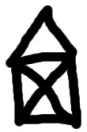
\includegraphics{tess_house.png}

\item {} 
Not all shapes like the one above can be drawn without lifting your pen, or going over
an edge more than once.  Which of these can be drawn?

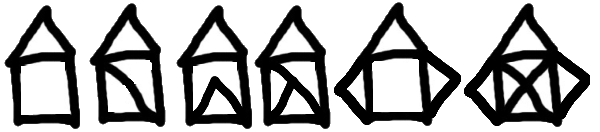
\includegraphics{tess_more_houses.png}

Now read Wikipedia's article(\href{http://en.wikipedia.org/wiki/Eulerian\_path}{http://en.wikipedia.org/wiki/Eulerian\_path}) about Eulerian paths.
Learn how to tell immediately by inspection whether it is possible to find a solution or not.
If the path is possible, you'll also know where to put your pen to start drawing, and where
you should end up!

\item {} 
What will \code{num\_digits(0)} return? Modify it to return \code{1} for this
case. Why does a call to \code{num\_digits(-24)} result in an infinite loop?
(\emph{hint: -1//10 evaluates to -1})  Modify \code{num\_digits} so that it works
correctly with any integer value. Add these tests:

\begin{Verbatim}[commandchars=\\\{\}]
\PYG{n}{test}\PYG{p}{(}\PYG{n}{num\PYGZus{}digits}\PYG{p}{(}\PYG{l+m+mi}{0}\PYG{p}{)}\PYG{p}{,} \PYG{l+m+mi}{1}\PYG{p}{)}
\PYG{n}{test}\PYG{p}{(}\PYG{n}{num\PYGZus{}digits}\PYG{p}{(}\PYG{o}{-}\PYG{l+m+mi}{12345}\PYG{p}{)}\PYG{p}{,} \PYG{l+m+mi}{5}\PYG{p}{)}
\end{Verbatim}

\item {} 
Write a function \code{num\_even\_digits(n)} that counts the number
of even digits in \code{n}.  These tests should pass:

\begin{Verbatim}[commandchars=\\\{\}]
\PYG{n}{test}\PYG{p}{(}\PYG{n}{num\PYGZus{}even\PYGZus{}digits}\PYG{p}{(}\PYG{l+m+mi}{123456}\PYG{p}{)}\PYG{p}{,} \PYG{l+m+mi}{3}\PYG{p}{)}
\PYG{n}{test}\PYG{p}{(}\PYG{n}{num\PYGZus{}even\PYGZus{}digits}\PYG{p}{(}\PYG{l+m+mi}{2468}\PYG{p}{)}\PYG{p}{,} \PYG{l+m+mi}{4}\PYG{p}{)}
\PYG{n}{test}\PYG{p}{(}\PYG{n}{num\PYGZus{}even\PYGZus{}digits}\PYG{p}{(}\PYG{l+m+mi}{1357}\PYG{p}{)}\PYG{p}{,} \PYG{l+m+mi}{0}\PYG{p}{)}
\PYG{n}{test}\PYG{p}{(}\PYG{n}{num\PYGZus{}even\PYGZus{}digits}\PYG{p}{(}\PYG{l+m+mi}{0}\PYG{p}{)}\PYG{p}{,} \PYG{l+m+mi}{1}\PYG{p}{)}
\end{Verbatim}

\item {} 
Write a function \code{sum\_of\_squares(xs)} that computes the sum
of the squares of the numbers in the list \code{xs}.  For example,
\code{sum\_of\_squares({[}2, 3, 4{]})} should return 4+9+16 which is 29:

\begin{Verbatim}[commandchars=\\\{\}]
\PYG{n}{test}\PYG{p}{(}\PYG{n}{sum\PYGZus{}of\PYGZus{}squares}\PYG{p}{(}\PYG{p}{[}\PYG{l+m+mi}{2}\PYG{p}{,} \PYG{l+m+mi}{3}\PYG{p}{,} \PYG{l+m+mi}{4}\PYG{p}{]}\PYG{p}{)}\PYG{p}{,} \PYG{l+m+mi}{29}\PYG{p}{)}
\PYG{n}{test}\PYG{p}{(}\PYG{n}{sum\PYGZus{}of\PYGZus{}squares}\PYG{p}{(}\PYG{p}{[} \PYG{p}{]}\PYG{p}{)}\PYG{p}{,} \PYG{l+m+mi}{0}\PYG{p}{)}
\PYG{n}{test}\PYG{p}{(}\PYG{n}{sum\PYGZus{}of\PYGZus{}squares}\PYG{p}{(}\PYG{p}{[}\PYG{l+m+mi}{2}\PYG{p}{,} \PYG{o}{-}\PYG{l+m+mi}{3}\PYG{p}{,} \PYG{l+m+mi}{4}\PYG{p}{]}\PYG{p}{)}\PYG{p}{,} \PYG{l+m+mi}{29}\PYG{p}{)}
\end{Verbatim}

\item {} 
You and your friend are in a team to write a two-player game,
human against computer, such as Tic-Tac-Toe / Noughts and Crosses.
Your friend will write the logic to play one round of the game, while you will
write the logic to allow many rounds of play, keep score, decide who
plays, first, etc.  The two of you negotiate on how the two parts of the
program will fit together, and you come up with this simple
scaffolding (which your friend will improve later):
\begin{quote}

\begin{Verbatim}[commandchars=\\\{\},numbers=left,firstnumber=1,stepnumber=1]
\PYG{c}{\PYGZsh{} Your friend will complete this function}
\PYG{k}{def} \PYG{n+nf}{play\PYGZus{}once}\PYG{p}{(}\PYG{n}{human\PYGZus{}plays\PYGZus{}first}\PYG{p}{)}\PYG{p}{:}
    \PYG{l+s+sd}{"""}
\PYG{l+s+sd}{       Must play one round of the game. If the parameter}
\PYG{l+s+sd}{       is True, the human gets to play first, else the}
\PYG{l+s+sd}{       computer gets to play first.  When the round ends,}
\PYG{l+s+sd}{       the return value of the function is one of}
\PYG{l+s+sd}{       -1 (human wins),  0 (game drawn),   1 (computer wins).}
\PYG{l+s+sd}{    """}
    \PYG{c}{\PYGZsh{} This is all dummy scaffolding code right at the moment...}
    \PYG{k+kn}{import} \PYG{n+nn}{random}                  \PYG{c}{\PYGZsh{} See Modules chapter ...}
    \PYG{n}{rng} \PYG{o}{=} \PYG{n}{random}\PYG{o}{.}\PYG{n}{Random}\PYG{p}{(}\PYG{p}{)}
    \PYG{c}{\PYGZsh{} Pick a random result between -1 and 1.}
    \PYG{n}{result} \PYG{o}{=} \PYG{n}{rng}\PYG{o}{.}\PYG{n}{randrange}\PYG{p}{(}\PYG{o}{-}\PYG{l+m+mi}{1}\PYG{p}{,}\PYG{l+m+mi}{2}\PYG{p}{)}
    \PYG{n+nb}{print}\PYG{p}{(}\PYG{l+s}{"}\PYG{l+s}{Human plays first=\PYGZob{}0\PYGZcb{},  winner=\PYGZob{}1\PYGZcb{} }\PYG{l+s}{"}
                       \PYG{o}{.}\PYG{n}{format}\PYG{p}{(}\PYG{n}{human\PYGZus{}plays\PYGZus{}first}\PYG{p}{,} \PYG{n}{result}\PYG{p}{)}\PYG{p}{)}
    \PYG{k}{return} \PYG{n}{result}
\end{Verbatim}
\end{quote}
\begin{enumerate}
\item {} 
Write the main program which repeatedly calls this function to play
the game, and after each round it announces the outcome as ``I win!'', ``You win!'', or ``Game drawn!''.
It then asks the player ``Do you want to play again?'' and either plays again,
or says ``Goodbye'', and terminates.

\item {} 
Keep score of how many wins each player has had, and how many draws there have been.
After each round of play, also announce the scores.

\item {} 
Add logic so that the players take turns to play first.

\item {} 
Compute the percentage of wins for the human, out of all games played.  Also announce this
at the end of each round.

\item {} 
Draw a flowchart of your logic.

\end{enumerate}

\end{enumerate}

\begin{DUlineblock}{0em}
\item[] 
\end{DUlineblock}


\chapter{Strings}
\label{strings::doc}\label{strings:strings}
\index{compound data type}\index{character}\index{subscript operator}\index{index}

\section{A compound data type}
\label{strings:index-0}\label{strings:a-compound-data-type}
So far we have seen built-in types like \code{int}, \code{float},
\code{bool}, \code{str} and we've seen lists and pairs.
Strings, lists, and pairs are qualitatively different from the others because they
are made up of smaller pieces.  In the case of strings, they're made up of smaller
strings each containing one \textbf{character}.

Types that comprise smaller pieces are called \textbf{compound data types}.
Depending on what we are doing, we may want to treat a compound data type as a
single thing, or we may want to access its parts. This ambiguity is useful.


\section{Working with strings as single things}
\label{strings:working-with-strings-as-single-things}
We previously saw that each turtle instance has its own attributes and
a number of methods that can be applied to the instance.  For example,
we could set the turtle's color, and we wrote \code{tess.turn(90)}.

Just like a turtle, a string is also an object.  So each string instance
has its own attributes and methods.

For example:
\begin{quote}

\begin{Verbatim}[commandchars=\\\{\}]
\PYG{g+gp}{\PYGZgt{}\PYGZgt{}\PYGZgt{} }\PYG{n}{ss} \PYG{o}{=} \PYG{l+s}{"}\PYG{l+s}{Hello, World!}\PYG{l+s}{"}
\PYG{g+gp}{\PYGZgt{}\PYGZgt{}\PYGZgt{} }\PYG{n}{tt} \PYG{o}{=} \PYG{n}{ss}\PYG{o}{.}\PYG{n}{upper}\PYG{p}{(}\PYG{p}{)}
\PYG{g+gp}{\PYGZgt{}\PYGZgt{}\PYGZgt{} }\PYG{n}{tt}
\PYG{g+go}{'HELLO, WORLD!'}
\end{Verbatim}
\end{quote}

\code{upper} is a method that can be invoked on any string object
to create a new string, in which all the
characters are in uppercase.  (The original string \code{ss} remains unchanged.)

There are also methods such as \code{lower}, \code{capitalize}, and
\code{swapcase} that do other interesting stuff.

To learn what methods are available, you can consult the Help documentation, look for
string methods, and read the documentation.  Or, if you're a bit lazier,
simply type the following into a PyScripter script:
\begin{quote}

\begin{Verbatim}[commandchars=\\\{\},numbers=left,firstnumber=1,stepnumber=1]
\PYG{n}{ss} \PYG{o}{=} \PYG{l+s}{"}\PYG{l+s}{Hello, World!}\PYG{l+s}{"}
\PYG{n}{tt} \PYG{o}{=} \PYG{n}{ss}\PYG{o}{.}
\end{Verbatim}
\end{quote}

When you type the period to select one of the methods of \code{ss}, PyScripter will pop up a
selection window showing all the methods (there are around 70 of them --- thank goodness we'll only
use a few of those!) that could be used on your string.
\begin{quote}

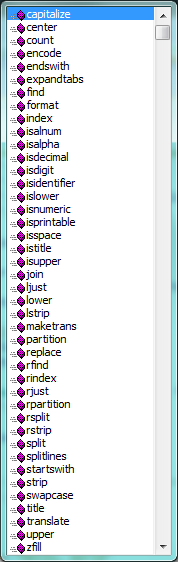
\includegraphics{string_methods.png}
\end{quote}

When you type the name of the method, some further help about its parameter and return
type, and its docstring, will be displayed.  This is a good example of a tool --- PyScripter ---
using the meta-information --- the docstrings --- provided by the module programmers.
\begin{quote}

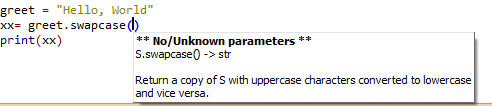
\includegraphics{swapcase.png}
\end{quote}


\section{Working with the parts of a string}
\label{strings:working-with-the-parts-of-a-string}
The \textbf{indexing operator} (Python uses square brackets to enclose the index)
selects a single character substring from a string:
\begin{quote}

\begin{Verbatim}[commandchars=\\\{\}]
\PYG{g+gp}{\PYGZgt{}\PYGZgt{}\PYGZgt{} }\PYG{n}{fruit} \PYG{o}{=} \PYG{l+s}{"}\PYG{l+s}{banana}\PYG{l+s}{"}
\PYG{g+gp}{\PYGZgt{}\PYGZgt{}\PYGZgt{} }\PYG{n}{m} \PYG{o}{=} \PYG{n}{fruit}\PYG{p}{[}\PYG{l+m+mi}{1}\PYG{p}{]}
\PYG{g+gp}{\PYGZgt{}\PYGZgt{}\PYGZgt{} }\PYG{n+nb}{print}\PYG{p}{(}\PYG{n}{m}\PYG{p}{)}
\end{Verbatim}
\end{quote}

The expression \code{fruit{[}1{]}} selects character number 1 from \code{fruit}, and creates a new
string containing just this one character. The variable \code{m} refers to the result.
When we display \code{m}, we could get a surprise:
\begin{quote}

\begin{Verbatim}[commandchars=\\\{\}]
\PYG{g+go}{a}
\end{Verbatim}
\end{quote}

Computer scientists always start counting
from zero! The letter at subscript position zero of \code{"banana"} is \code{b}.  So at
position \code{{[}1{]}} we have the letter \code{a}.

If we want to access the zero-eth letter of a string, we just place 0,
or any expression that evaluates to 0, inbetween the brackets:
\begin{quote}

\begin{Verbatim}[commandchars=\\\{\}]
\PYG{g+gp}{\PYGZgt{}\PYGZgt{}\PYGZgt{} }\PYG{n}{m} \PYG{o}{=} \PYG{n}{fruit}\PYG{p}{[}\PYG{l+m+mi}{0}\PYG{p}{]}
\PYG{g+gp}{\PYGZgt{}\PYGZgt{}\PYGZgt{} }\PYG{n+nb}{print}\PYG{p}{(}\PYG{n}{m}\PYG{p}{)}
\PYG{g+go}{b}
\end{Verbatim}
\end{quote}

The expression in brackets is called an \textbf{index}. An index specifies a member
of an ordered collection, in this case the collection of characters in the string. The index
\emph{indicates} which one you want, hence the name. It can be any integer
expression.

We can use \code{enumerate} to visualize the indices:
\begin{quote}

\begin{Verbatim}[commandchars=\\\{\}]
\PYG{g+gp}{\PYGZgt{}\PYGZgt{}\PYGZgt{} }\PYG{n}{fruit} \PYG{o}{=} \PYG{l+s}{"}\PYG{l+s}{banana}\PYG{l+s}{"}
\PYG{g+gp}{\PYGZgt{}\PYGZgt{}\PYGZgt{} }\PYG{n+nb}{list}\PYG{p}{(}\PYG{n+nb}{enumerate}\PYG{p}{(}\PYG{n}{fruit}\PYG{p}{)}\PYG{p}{)}
\PYG{g+go}{[(0, 'b'), (1, 'a'), (2, 'n'), (3, 'a'), (4, 'n'), (5, 'a')]}
\end{Verbatim}
\end{quote}

Do not worry about \code{enumerate} at this point, we will see more of it
in the chapter on lists.

Note that indexing returns a \emph{string} --- Python has no special type for a single character.
It is just a string of length 1.

We've also seen lists previously.  The same indexing notation works to extract elements from
a list:
\begin{quote}

\begin{Verbatim}[commandchars=\\\{\}]
\PYG{g+gp}{\PYGZgt{}\PYGZgt{}\PYGZgt{} }\PYG{n}{prime\PYGZus{}nums} \PYG{o}{=} \PYG{p}{[}\PYG{l+m+mi}{2}\PYG{p}{,} \PYG{l+m+mi}{3}\PYG{p}{,} \PYG{l+m+mi}{5}\PYG{p}{,} \PYG{l+m+mi}{7}\PYG{p}{,} \PYG{l+m+mi}{11}\PYG{p}{,} \PYG{l+m+mi}{13}\PYG{p}{,} \PYG{l+m+mi}{17}\PYG{p}{,} \PYG{l+m+mi}{19}\PYG{p}{,} \PYG{l+m+mi}{23}\PYG{p}{,} \PYG{l+m+mi}{29}\PYG{p}{,} \PYG{l+m+mi}{31}\PYG{p}{]}
\PYG{g+gp}{\PYGZgt{}\PYGZgt{}\PYGZgt{} }\PYG{n}{prime\PYGZus{}nums}\PYG{p}{[}\PYG{l+m+mi}{4}\PYG{p}{]}
\PYG{g+go}{11}
\PYG{g+gp}{\PYGZgt{}\PYGZgt{}\PYGZgt{} }\PYG{n}{friends} \PYG{o}{=} \PYG{p}{[}\PYG{l+s}{"}\PYG{l+s}{Joe}\PYG{l+s}{"}\PYG{p}{,} \PYG{l+s}{"}\PYG{l+s}{Zoe}\PYG{l+s}{"}\PYG{p}{,} \PYG{l+s}{"}\PYG{l+s}{Brad}\PYG{l+s}{"}\PYG{p}{,} \PYG{l+s}{"}\PYG{l+s}{Angelina}\PYG{l+s}{"}\PYG{p}{,} \PYG{l+s}{"}\PYG{l+s}{Zuki}\PYG{l+s}{"}\PYG{p}{,} \PYG{l+s}{"}\PYG{l+s}{Thandi}\PYG{l+s}{"}\PYG{p}{,} \PYG{l+s}{"}\PYG{l+s}{Paris}\PYG{l+s}{"}\PYG{p}{]}
\PYG{g+gp}{\PYGZgt{}\PYGZgt{}\PYGZgt{} }\PYG{n}{friends}\PYG{p}{[}\PYG{l+m+mi}{3}\PYG{p}{]}
\PYG{g+go}{'Angelina'}
\end{Verbatim}
\end{quote}

\index{len function}\index{function!len}\index{runtime error}\index{negative index}\index{index!negative}

\section{Length}
\label{strings:length}\label{strings:index-1}
The \code{len} function, when applied to a string, returns the number of characters in a string:
\begin{quote}

\begin{Verbatim}[commandchars=\\\{\}]
\PYG{g+gp}{\PYGZgt{}\PYGZgt{}\PYGZgt{} }\PYG{n}{fruit} \PYG{o}{=} \PYG{l+s}{"}\PYG{l+s}{banana}\PYG{l+s}{"}
\PYG{g+gp}{\PYGZgt{}\PYGZgt{}\PYGZgt{} }\PYG{n+nb}{len}\PYG{p}{(}\PYG{n}{fruit}\PYG{p}{)}
\PYG{g+go}{6}
\end{Verbatim}
\end{quote}

To get the last letter of a string, you might be tempted to try something like
this:
\begin{quote}

\begin{Verbatim}[commandchars=\\\{\},numbers=left,firstnumber=1,stepnumber=1]
\PYG{n}{sz} \PYG{o}{=} \PYG{n+nb}{len}\PYG{p}{(}\PYG{n}{fruit}\PYG{p}{)}
\PYG{n}{last} \PYG{o}{=} \PYG{n}{fruit}\PYG{p}{[}\PYG{n}{sz}\PYG{p}{]}       \PYG{c}{\PYGZsh{} ERROR!}
\end{Verbatim}
\end{quote}

That won't work. It causes the runtime error
\code{IndexError: string index out of range}. The reason is that there is no
character at index position 6 in \code{"banana"}.
Because we start counting at zero, the six indexes are
numbered 0 to 5. To get the last character, we have to subtract 1 from
the length of \code{fruit}:
\begin{quote}

\begin{Verbatim}[commandchars=\\\{\},numbers=left,firstnumber=1,stepnumber=1]
\PYG{n}{sz} \PYG{o}{=} \PYG{n+nb}{len}\PYG{p}{(}\PYG{n}{fruit}\PYG{p}{)}
\PYG{n}{last} \PYG{o}{=} \PYG{n}{fruit}\PYG{p}{[}\PYG{n}{sz}\PYG{o}{-}\PYG{l+m+mi}{1}\PYG{p}{]}
\end{Verbatim}
\end{quote}

Alternatively, we can use \textbf{negative indices}, which count backward from the
end of the string. The expression \code{fruit{[}-1{]}} yields the last letter,
\code{fruit{[}-2{]}} yields the second to last, and so on.

As you might have guessed, indexing with a negative index also works like this for lists.

We won't use negative indexes in the rest of these notes --- not many computer languages
use this idiom, and you'll probably be better off avoiding it. But there is plenty of
Python code out on the Internet that will use this trick, so it is best to know that it exists.

\index{traversal}\index{for loop}\index{concatenation}\index{abecedarian series}
\index{McCloskey, Robert}\index{Make Way for Ducklings}

\section{Traversal and the \texttt{for} loop}
\label{strings:traversal-and-the-for-loop}\label{strings:index-3}
A lot of computations involve processing a string one character at a time.
Often they start at the beginning, select each character in turn, do something
to it, and continue until the end. This pattern of processing is called a
\textbf{traversal}. One way to encode a traversal is with a \code{while} statement:
\begin{quote}

\begin{Verbatim}[commandchars=\\\{\},numbers=left,firstnumber=1,stepnumber=1]
\PYG{n}{ix} \PYG{o}{=} \PYG{l+m+mi}{0}
\PYG{k}{while} \PYG{n}{ix} \PYG{o}{\PYGZlt{}} \PYG{n+nb}{len}\PYG{p}{(}\PYG{n}{fruit}\PYG{p}{)}\PYG{p}{:}
    \PYG{n}{letter} \PYG{o}{=} \PYG{n}{fruit}\PYG{p}{[}\PYG{n}{ix}\PYG{p}{]}
    \PYG{n+nb}{print}\PYG{p}{(}\PYG{n}{letter}\PYG{p}{)}
    \PYG{n}{ix} \PYG{o}{+}\PYG{o}{=} \PYG{l+m+mi}{1}
\end{Verbatim}
\end{quote}

This loop traverses the string and displays each letter on a line by itself.
The loop condition is \code{ix \textless{} len(fruit)}, so when \code{ix} is equal to the
length of the string, the condition is false, and the body of the loop is not
executed. The last character accessed is the one with the index
\code{len(fruit)-1}, which is the last character in the string.

But we've previously seen how the \code{for} loop can easily iterate over
the elements in a list and it can do so for strings as well:
\begin{quote}

\begin{Verbatim}[commandchars=\\\{\},numbers=left,firstnumber=1,stepnumber=1]
\PYG{k}{for} \PYG{n}{c} \PYG{o+ow}{in} \PYG{n}{fruit}\PYG{p}{:}
    \PYG{n+nb}{print}\PYG{p}{(}\PYG{n}{c}\PYG{p}{)}
\end{Verbatim}
\end{quote}

Each time through the loop, the next character in the string is assigned to the
variable \code{c}. The loop continues until no characters are left. Here we
can see the expressive power the \code{for} loop gives us compared to the
while loop when traversing a string.

The following example shows how to use concatenation and a \code{for} loop to
generate an abecedarian series. Abecedarian refers to a series or list in which
the elements appear in alphabetical order. For example, in Robert McCloskey's
book \emph{Make Way for Ducklings}, the names of the ducklings are Jack, Kack, Lack,
Mack, Nack, Ouack, Pack, and Quack.  This loop outputs these names in order:
\begin{quote}

\begin{Verbatim}[commandchars=\\\{\},numbers=left,firstnumber=1,stepnumber=1]
\PYG{n}{prefixes} \PYG{o}{=} \PYG{l+s}{"}\PYG{l+s}{JKLMNOPQ}\PYG{l+s}{"}
\PYG{n}{suffix} \PYG{o}{=} \PYG{l+s}{"}\PYG{l+s}{ack}\PYG{l+s}{"}

\PYG{k}{for} \PYG{n}{p} \PYG{o+ow}{in} \PYG{n}{prefixes}\PYG{p}{:}
    \PYG{n+nb}{print}\PYG{p}{(}\PYG{n}{p} \PYG{o}{+} \PYG{n}{suffix}\PYG{p}{)}
\end{Verbatim}
\end{quote}

The output of this program is:
\begin{quote}

\begin{Verbatim}[commandchars=\\\{\}]
\PYG{g+go}{Jack}
\PYG{g+go}{Kack}
\PYG{g+go}{Lack}
\PYG{g+go}{Mack}
\PYG{g+go}{Nack}
\PYG{g+go}{Oack}
\PYG{g+go}{Pack}
\PYG{g+go}{Qack}
\end{Verbatim}
\end{quote}

Of course, that's not quite right because Ouack and Quack are misspelled.
You'll fix this as an exercise below.

\index{slice}\index{string slice}\index{substring}\index{sublist}

\section{Slices}
\label{strings:index-4}\label{strings:slices}
A \emph{substring} of a string is obtained by taking a \textbf{slice}.   Similarly, we can
slice a list to refer to some sublist of the items in the list:
\begin{quote}

\begin{Verbatim}[commandchars=\\\{\}]
\PYG{g+gp}{\PYGZgt{}\PYGZgt{}\PYGZgt{} }\PYG{n}{s} \PYG{o}{=} \PYG{l+s}{"}\PYG{l+s}{Peter, Paul, and Mary}\PYG{l+s}{"}
\PYG{g+gp}{\PYGZgt{}\PYGZgt{}\PYGZgt{} }\PYG{n+nb}{print}\PYG{p}{(}\PYG{n}{s}\PYG{p}{[}\PYG{l+m+mi}{0}\PYG{p}{:}\PYG{l+m+mi}{5}\PYG{p}{]}\PYG{p}{)}
\PYG{g+go}{Peter}
\PYG{g+gp}{\PYGZgt{}\PYGZgt{}\PYGZgt{} }\PYG{n+nb}{print}\PYG{p}{(}\PYG{n}{s}\PYG{p}{[}\PYG{l+m+mi}{7}\PYG{p}{:}\PYG{l+m+mi}{11}\PYG{p}{]}\PYG{p}{)}
\PYG{g+go}{Paul}
\PYG{g+gp}{\PYGZgt{}\PYGZgt{}\PYGZgt{} }\PYG{n+nb}{print}\PYG{p}{(}\PYG{n}{s}\PYG{p}{[}\PYG{l+m+mi}{17}\PYG{p}{:}\PYG{l+m+mi}{21}\PYG{p}{]}\PYG{p}{)}
\PYG{g+go}{Mary}
\PYG{g+gp}{\PYGZgt{}\PYGZgt{}\PYGZgt{} }\PYG{n}{friends} \PYG{o}{=} \PYG{p}{[}\PYG{l+s}{"}\PYG{l+s}{Joe}\PYG{l+s}{"}\PYG{p}{,} \PYG{l+s}{"}\PYG{l+s}{Zoe}\PYG{l+s}{"}\PYG{p}{,} \PYG{l+s}{"}\PYG{l+s}{Brad}\PYG{l+s}{"}\PYG{p}{,} \PYG{l+s}{"}\PYG{l+s}{Angelina}\PYG{l+s}{"}\PYG{p}{,} \PYG{l+s}{"}\PYG{l+s}{Zuki}\PYG{l+s}{"}\PYG{p}{,} \PYG{l+s}{"}\PYG{l+s}{Thandi}\PYG{l+s}{"}\PYG{p}{,} \PYG{l+s}{"}\PYG{l+s}{Paris}\PYG{l+s}{"}\PYG{p}{]}
\PYG{g+gp}{\PYGZgt{}\PYGZgt{}\PYGZgt{} }\PYG{n+nb}{print}\PYG{p}{(}\PYG{n}{friends}\PYG{p}{[}\PYG{l+m+mi}{2}\PYG{p}{:}\PYG{l+m+mi}{4}\PYG{p}{]}\PYG{p}{)}
\PYG{g+go}{['Brad', 'Angelina']}
\end{Verbatim}
\end{quote}

The operator \code{{[}n:m{]}} returns the part of the string from the n'th character
to the m'th character, including the first but excluding the last. This
behavior makes sense if you imagine the indices
pointing \emph{between} the characters, as in the following diagram:
\begin{quote}

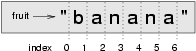
\includegraphics{banana.png}
\end{quote}

Now if you imagine this as a piece of paper, the slice operator \code{{[}n:m{]}} cuts
the paper at the \code{n} and \code{m} positions.

Two tricks are added to this: if you omit the first index (before the colon),
the slice starts at the beginning of the string (or list). If you omit the second index,
the slice extends to the end of the string (or list). Thus:
\begin{quote}

\begin{Verbatim}[commandchars=\\\{\}]
\PYG{g+gp}{\PYGZgt{}\PYGZgt{}\PYGZgt{} }\PYG{n}{fruit} \PYG{o}{=} \PYG{l+s}{"}\PYG{l+s}{banana}\PYG{l+s}{"}
\PYG{g+gp}{\PYGZgt{}\PYGZgt{}\PYGZgt{} }\PYG{n}{fruit}\PYG{p}{[}\PYG{p}{:}\PYG{l+m+mi}{3}\PYG{p}{]}
\PYG{g+go}{'ban'}
\PYG{g+gp}{\PYGZgt{}\PYGZgt{}\PYGZgt{} }\PYG{n}{fruit}\PYG{p}{[}\PYG{l+m+mi}{3}\PYG{p}{:}\PYG{p}{]}
\PYG{g+go}{'ana'}
\end{Verbatim}
\end{quote}

What do you think \code{s{[}:{]}} means?   What about \code{friends{[}4:{]}}?

\index{string comparison}\index{comparison of strings}

\section{String comparison}
\label{strings:index-5}\label{strings:string-comparison}
The comparison operators work on strings. To see if two strings are equal:
\begin{quote}

\begin{Verbatim}[commandchars=\\\{\},numbers=left,firstnumber=1,stepnumber=1]
\PYG{k}{if} \PYG{n}{word} \PYG{o}{==} \PYG{l+s}{"}\PYG{l+s}{banana}\PYG{l+s}{"}\PYG{p}{:}
    \PYG{n+nb}{print}\PYG{p}{(}\PYG{l+s}{"}\PYG{l+s}{Yes, we have no bananas!}\PYG{l+s}{"}\PYG{p}{)}
\end{Verbatim}
\end{quote}

Other comparison operations are useful for putting words in
\emph{lexicographical} order:
\begin{quote}

\begin{Verbatim}[commandchars=\\\{\},numbers=left,firstnumber=1,stepnumber=1]
\PYG{k}{if} \PYG{n}{word} \PYG{o}{\PYGZlt{}} \PYG{l+s}{"}\PYG{l+s}{banana}\PYG{l+s}{"}\PYG{p}{:}
    \PYG{n+nb}{print}\PYG{p}{(}\PYG{l+s}{"}\PYG{l+s}{Your word, }\PYG{l+s}{"} \PYG{o}{+} \PYG{n}{word} \PYG{o}{+} \PYG{l+s}{"}\PYG{l+s}{, comes before banana.}\PYG{l+s}{"}\PYG{p}{)}
\PYG{k}{elif} \PYG{n}{word} \PYG{o}{\PYGZgt{}} \PYG{l+s}{"}\PYG{l+s}{banana}\PYG{l+s}{"}\PYG{p}{:}
    \PYG{n+nb}{print}\PYG{p}{(}\PYG{l+s}{"}\PYG{l+s}{Your word, }\PYG{l+s}{"} \PYG{o}{+} \PYG{n}{word} \PYG{o}{+} \PYG{l+s}{"}\PYG{l+s}{, comes after banana.}\PYG{l+s}{"}\PYG{p}{)}
\PYG{k}{else}\PYG{p}{:}
    \PYG{n+nb}{print}\PYG{p}{(}\PYG{l+s}{"}\PYG{l+s}{Yes, we have no bananas!}\PYG{l+s}{"}\PYG{p}{)}
\end{Verbatim}
\end{quote}

This is similar to the alphabetical order you would use with a dictionary,
except that all the uppercase letters come before all the lowercase letters. As
a result:
\begin{quote}

\begin{Verbatim}[commandchars=\\\{\}]
\PYG{g+go}{Your word, Zebra, comes before banana.}
\end{Verbatim}
\end{quote}

A common way to address this problem is to convert strings to a standard
format, such as all lowercase, before performing the comparison. A more
difficult problem is making the program realize that zebras are not fruit.

\index{mutable}\index{immutable}\index{runtime error}

\section{Strings are immutable}
\label{strings:index-6}\label{strings:strings-are-immutable}
It is tempting to use the \code{{[}{]}} operator on the left side of an assignment,
with the intention of changing a character in a string.  For example:
\begin{quote}

\begin{Verbatim}[commandchars=\\\{\},numbers=left,firstnumber=1,stepnumber=1]
\PYG{n}{greeting} \PYG{o}{=} \PYG{l+s}{"}\PYG{l+s}{Hello, world!}\PYG{l+s}{"}
\PYG{n}{greeting}\PYG{p}{[}\PYG{l+m+mi}{0}\PYG{p}{]} \PYG{o}{=} \PYG{l+s}{'}\PYG{l+s}{J}\PYG{l+s}{'}            \PYG{c}{\PYGZsh{} ERROR!}
\PYG{n+nb}{print}\PYG{p}{(}\PYG{n}{greeting}\PYG{p}{)}
\end{Verbatim}
\end{quote}

Instead of producing the output \code{Jello, world!}, this code produces the
runtime error \code{TypeError: 'str' object does not support item assignment}.

Strings are \textbf{immutable}, which means you can't change an existing string. The
best you can do is create a new string that is a variation on the original:
\begin{quote}

\begin{Verbatim}[commandchars=\\\{\},numbers=left,firstnumber=1,stepnumber=1]
\PYG{n}{greeting} \PYG{o}{=} \PYG{l+s}{"}\PYG{l+s}{Hello, world!}\PYG{l+s}{"}
\PYG{n}{new\PYGZus{}greeting} \PYG{o}{=} \PYG{l+s}{"}\PYG{l+s}{J}\PYG{l+s}{"} \PYG{o}{+} \PYG{n}{greeting}\PYG{p}{[}\PYG{l+m+mi}{1}\PYG{p}{:}\PYG{p}{]}
\PYG{n+nb}{print}\PYG{p}{(}\PYG{n}{new\PYGZus{}greeting}\PYG{p}{)}
\end{Verbatim}
\end{quote}

The solution here is to concatenate a new first letter onto a slice of
\code{greeting}. This operation has no effect on the original string.

\index{in operator}\index{operator!in}

\section{The \texttt{in} and \texttt{not in} operators}
\label{strings:index-7}\label{strings:the-in-and-not-in-operators}
The \code{in} operator tests for membership. When both of the arguments to \code{in}
are strings, \code{in} checks whether the left argument is a substring of the right
argument.
\begin{quote}

\begin{Verbatim}[commandchars=\\\{\}]
\PYG{g+gp}{\PYGZgt{}\PYGZgt{}\PYGZgt{} }\PYG{l+s}{"}\PYG{l+s}{p}\PYG{l+s}{"} \PYG{o+ow}{in} \PYG{l+s}{"}\PYG{l+s}{apple}\PYG{l+s}{"}
\PYG{g+go}{True}
\PYG{g+gp}{\PYGZgt{}\PYGZgt{}\PYGZgt{} }\PYG{l+s}{"}\PYG{l+s}{i}\PYG{l+s}{"} \PYG{o+ow}{in} \PYG{l+s}{"}\PYG{l+s}{apple}\PYG{l+s}{"}
\PYG{g+go}{False}
\PYG{g+gp}{\PYGZgt{}\PYGZgt{}\PYGZgt{} }\PYG{l+s}{"}\PYG{l+s}{ap}\PYG{l+s}{"} \PYG{o+ow}{in} \PYG{l+s}{"}\PYG{l+s}{apple}\PYG{l+s}{"}
\PYG{g+go}{True}
\PYG{g+gp}{\PYGZgt{}\PYGZgt{}\PYGZgt{} }\PYG{l+s}{"}\PYG{l+s}{pa}\PYG{l+s}{"} \PYG{o+ow}{in} \PYG{l+s}{"}\PYG{l+s}{apple}\PYG{l+s}{"}
\PYG{g+go}{False}
\end{Verbatim}
\end{quote}

Note that a string is a substring of itself, and the empty string is a
substring of any other string. (Also note that computer scientists
like to think about these edge cases quite carefully!)
\begin{quote}

\begin{Verbatim}[commandchars=\\\{\}]
\PYG{g+gp}{\PYGZgt{}\PYGZgt{}\PYGZgt{} }\PYG{l+s}{"}\PYG{l+s}{a}\PYG{l+s}{"} \PYG{o+ow}{in} \PYG{l+s}{"}\PYG{l+s}{a}\PYG{l+s}{"}
\PYG{g+go}{True}
\PYG{g+gp}{\PYGZgt{}\PYGZgt{}\PYGZgt{} }\PYG{l+s}{"}\PYG{l+s}{apple}\PYG{l+s}{"} \PYG{o+ow}{in} \PYG{l+s}{"}\PYG{l+s}{apple}\PYG{l+s}{"}
\PYG{g+go}{True}
\PYG{g+gp}{\PYGZgt{}\PYGZgt{}\PYGZgt{} }\PYG{l+s}{"}\PYG{l+s}{"} \PYG{o+ow}{in} \PYG{l+s}{"}\PYG{l+s}{a}\PYG{l+s}{"}
\PYG{g+go}{True}
\PYG{g+gp}{\PYGZgt{}\PYGZgt{}\PYGZgt{} }\PYG{l+s}{"}\PYG{l+s}{"} \PYG{o+ow}{in} \PYG{l+s}{"}\PYG{l+s}{apple}\PYG{l+s}{"}
\PYG{g+go}{True}
\end{Verbatim}
\end{quote}

The \code{not in} operator returns the logical opposite results of \code{in}:
\begin{quote}

\begin{Verbatim}[commandchars=\\\{\}]
\PYG{g+gp}{\PYGZgt{}\PYGZgt{}\PYGZgt{} }\PYG{l+s}{"}\PYG{l+s}{x}\PYG{l+s}{"} \PYG{o+ow}{not} \PYG{o+ow}{in} \PYG{l+s}{"}\PYG{l+s}{apple}\PYG{l+s}{"}
\PYG{g+go}{True}
\end{Verbatim}
\end{quote}

Combining the \code{in} operator with string concatenation using \code{+}, we can
write a function that removes all the vowels from a string:
\begin{quote}

\begin{Verbatim}[commandchars=\\\{\},numbers=left,firstnumber=1,stepnumber=1]
\PYG{k}{def} \PYG{n+nf}{remove\PYGZus{}vowels}\PYG{p}{(}\PYG{n}{s}\PYG{p}{)}\PYG{p}{:}
    \PYG{n}{vowels} \PYG{o}{=} \PYG{l+s}{"}\PYG{l+s}{aeiouAEIOU}\PYG{l+s}{"}
    \PYG{n}{s\PYGZus{}sans\PYGZus{}vowels} \PYG{o}{=} \PYG{l+s}{"}\PYG{l+s}{"}
    \PYG{k}{for} \PYG{n}{x} \PYG{o+ow}{in} \PYG{n}{s}\PYG{p}{:}
        \PYG{k}{if} \PYG{n}{x} \PYG{o+ow}{not} \PYG{o+ow}{in} \PYG{n}{vowels}\PYG{p}{:}
            \PYG{n}{s\PYGZus{}sans\PYGZus{}vowels} \PYG{o}{+}\PYG{o}{=} \PYG{n}{x}
    \PYG{k}{return} \PYG{n}{s\PYGZus{}sans\PYGZus{}vowels}

\PYG{n}{test}\PYG{p}{(}\PYG{n}{remove\PYGZus{}vowels}\PYG{p}{(}\PYG{l+s}{"}\PYG{l+s}{compsci}\PYG{l+s}{"}\PYG{p}{)}\PYG{p}{,} \PYG{l+s}{"}\PYG{l+s}{cmpsc}\PYG{l+s}{"}\PYG{p}{)}
\PYG{n}{test}\PYG{p}{(}\PYG{n}{remove\PYGZus{}vowels}\PYG{p}{(}\PYG{l+s}{"}\PYG{l+s}{aAbEefIijOopUus}\PYG{l+s}{"}\PYG{p}{)}\PYG{p}{,} \PYG{l+s}{"}\PYG{l+s}{bfjps}\PYG{l+s}{"}\PYG{p}{)}
\end{Verbatim}
\end{quote}

\index{traversal}\index{eureka traversal}\index{short-circuit evaluation}\index{pattern of computation}\index{computation pattern}

\section{A \texttt{find} function}
\label{strings:index-8}\label{strings:a-find-function}
What does the following function do?
\begin{quote}

\begin{Verbatim}[commandchars=\\\{\},numbers=left,firstnumber=1,stepnumber=1]
\PYG{k}{def} \PYG{n+nf}{find}\PYG{p}{(}\PYG{n}{strng}\PYG{p}{,} \PYG{n}{ch}\PYG{p}{)}\PYG{p}{:}
    \PYG{l+s+sd}{"""}
\PYG{l+s+sd}{      Find and return the index of ch in strng.}
\PYG{l+s+sd}{      Return -1 if ch does not occur in strng.}
\PYG{l+s+sd}{    """}
    \PYG{n}{ix} \PYG{o}{=} \PYG{l+m+mi}{0}
    \PYG{k}{while} \PYG{n}{ix} \PYG{o}{\PYGZlt{}} \PYG{n+nb}{len}\PYG{p}{(}\PYG{n}{strng}\PYG{p}{)}\PYG{p}{:}
        \PYG{k}{if} \PYG{n}{strng}\PYG{p}{[}\PYG{n}{ix}\PYG{p}{]} \PYG{o}{==} \PYG{n}{ch}\PYG{p}{:}
            \PYG{k}{return} \PYG{n}{ix}
        \PYG{n}{ix} \PYG{o}{+}\PYG{o}{=} \PYG{l+m+mi}{1}
    \PYG{k}{return} \PYG{o}{-}\PYG{l+m+mi}{1}

\PYG{n}{test}\PYG{p}{(}\PYG{n}{find}\PYG{p}{(}\PYG{l+s}{"}\PYG{l+s}{Compsci}\PYG{l+s}{"}\PYG{p}{,} \PYG{l+s}{"}\PYG{l+s}{p}\PYG{l+s}{"}\PYG{p}{)}\PYG{p}{,} \PYG{l+m+mi}{3}\PYG{p}{)}
\PYG{n}{test}\PYG{p}{(}\PYG{n}{find}\PYG{p}{(}\PYG{l+s}{"}\PYG{l+s}{Compsci}\PYG{l+s}{"}\PYG{p}{,} \PYG{l+s}{"}\PYG{l+s}{C}\PYG{l+s}{"}\PYG{p}{)}\PYG{p}{,} \PYG{l+m+mi}{0}\PYG{p}{)}
\PYG{n}{test}\PYG{p}{(}\PYG{n}{find}\PYG{p}{(}\PYG{l+s}{"}\PYG{l+s}{Compsci}\PYG{l+s}{"}\PYG{p}{,} \PYG{l+s}{"}\PYG{l+s}{i}\PYG{l+s}{"}\PYG{p}{)}\PYG{p}{,} \PYG{l+m+mi}{6}\PYG{p}{)}
\PYG{n}{test}\PYG{p}{(}\PYG{n}{find}\PYG{p}{(}\PYG{l+s}{"}\PYG{l+s}{Compsci}\PYG{l+s}{"}\PYG{p}{,} \PYG{l+s}{"}\PYG{l+s}{x}\PYG{l+s}{"}\PYG{p}{)}\PYG{p}{,} \PYG{o}{-}\PYG{l+m+mi}{1}\PYG{p}{)}
\end{Verbatim}
\end{quote}

In a sense, \code{find} is the opposite of the indexing operator. Instead of taking
an index and extracting the corresponding character, it takes a character and
finds the index where that character appears. If the character is not found,
the function returns \code{-1}.

This is another example where we see a \code{return} statement inside a loop.
If \code{strng{[}ix{]} == ch}, the function returns immediately, breaking out of
the loop prematurely.

If the character doesn't appear in the string, then the program exits the loop
normally and returns \code{-1}.

This pattern of computation is sometimes called a \textbf{eureka traversal} or
\textbf{short-circuit evaluation},  because as soon as we find what we are looking for,
we can cry ``Eureka!'', take the short-circuit, and stop looking.

\index{counting pattern}

\section{Looping and counting}
\label{strings:looping-and-counting}\label{strings:index-9}
The following program counts the number of times the letter \code{a} appears in a
string, and is another example of the counter pattern introduced in
{\hyperref[iteration:counting]{\emph{Counting digits}}}:
\begin{quote}

\begin{Verbatim}[commandchars=\\\{\},numbers=left,firstnumber=1,stepnumber=1]
\PYG{k}{def} \PYG{n+nf}{count\PYGZus{}a}\PYG{p}{(}\PYG{n}{text}\PYG{p}{)}\PYG{p}{:}
    \PYG{n}{count} \PYG{o}{=} \PYG{l+m+mi}{0}
    \PYG{k}{for} \PYG{n}{c} \PYG{o+ow}{in} \PYG{n}{text}\PYG{p}{:}
        \PYG{k}{if} \PYG{n}{c} \PYG{o}{==} \PYG{l+s}{"}\PYG{l+s}{a}\PYG{l+s}{"}\PYG{p}{:}
            \PYG{n}{count} \PYG{o}{+}\PYG{o}{=} \PYG{l+m+mi}{1}
    \PYG{k}{return}\PYG{p}{(}\PYG{n}{count}\PYG{p}{)}

\PYG{n}{test}\PYG{p}{(}\PYG{n}{count\PYGZus{}a}\PYG{p}{(}\PYG{l+s}{"}\PYG{l+s}{banana}\PYG{l+s}{"}\PYG{p}{)}\PYG{p}{,} \PYG{l+m+mi}{3}\PYG{p}{)}
\end{Verbatim}
\end{quote}

\index{optional parameter}\index{default value}\index{parameter!optional}

\section{Optional parameters}
\label{strings:optional-parameters}\label{strings:index-10}\label{strings:id1}
To find the locations of the second or third occurrence of a character in a
string, we can modify the \code{find} function, adding a third parameter for the
starting position in the search string:
\begin{quote}

\begin{Verbatim}[commandchars=\\\{\},numbers=left,firstnumber=1,stepnumber=1]
\PYG{k}{def} \PYG{n+nf}{find2}\PYG{p}{(}\PYG{n}{strng}\PYG{p}{,} \PYG{n}{ch}\PYG{p}{,} \PYG{n}{start}\PYG{p}{)}\PYG{p}{:}
    \PYG{n}{ix} \PYG{o}{=} \PYG{n}{start}
    \PYG{k}{while} \PYG{n}{ix} \PYG{o}{\PYGZlt{}} \PYG{n+nb}{len}\PYG{p}{(}\PYG{n}{strng}\PYG{p}{)}\PYG{p}{:}
        \PYG{k}{if} \PYG{n}{strng}\PYG{p}{[}\PYG{n}{ix}\PYG{p}{]} \PYG{o}{==} \PYG{n}{ch}\PYG{p}{:}
            \PYG{k}{return} \PYG{n}{ix}
        \PYG{n}{ix} \PYG{o}{+}\PYG{o}{=} \PYG{l+m+mi}{1}
    \PYG{k}{return} \PYG{o}{-}\PYG{l+m+mi}{1}

\PYG{n}{test}\PYG{p}{(}\PYG{n}{find2}\PYG{p}{(}\PYG{l+s}{"}\PYG{l+s}{banana}\PYG{l+s}{"}\PYG{p}{,} \PYG{l+s}{"}\PYG{l+s}{a}\PYG{l+s}{"}\PYG{p}{,} \PYG{l+m+mi}{2}\PYG{p}{)}\PYG{p}{,} \PYG{l+m+mi}{3}\PYG{p}{)}
\end{Verbatim}
\end{quote}

The call \code{find2("banana", "a", 2)} now returns \code{3}, the index of the first
occurrence of ``a'' in ``banana'' starting the search at index 2. What does
\code{find2("banana", "n", 3)} return? If you said, 4, there is a good chance you
understand how \code{find2} works.

Better still, we can combine \code{find} and \code{find2} using an
\textbf{optional parameter}:
\begin{quote}

\begin{Verbatim}[commandchars=\\\{\},numbers=left,firstnumber=1,stepnumber=1]
\PYG{k}{def} \PYG{n+nf}{find}\PYG{p}{(}\PYG{n}{strng}\PYG{p}{,} \PYG{n}{ch}\PYG{p}{,} \PYG{n}{start}\PYG{o}{=}\PYG{l+m+mi}{0}\PYG{p}{)}\PYG{p}{:}
    \PYG{n}{ix} \PYG{o}{=} \PYG{n}{start}
    \PYG{k}{while} \PYG{n}{ix} \PYG{o}{\PYGZlt{}} \PYG{n+nb}{len}\PYG{p}{(}\PYG{n}{strng}\PYG{p}{)}\PYG{p}{:}
        \PYG{k}{if} \PYG{n}{strng}\PYG{p}{[}\PYG{n}{ix}\PYG{p}{]} \PYG{o}{==} \PYG{n}{ch}\PYG{p}{:}
            \PYG{k}{return} \PYG{n}{ix}
        \PYG{n}{ix} \PYG{o}{+}\PYG{o}{=} \PYG{l+m+mi}{1}
    \PYG{k}{return} \PYG{o}{-}\PYG{l+m+mi}{1}
\end{Verbatim}
\end{quote}

When a function has an optional parameter, the caller \emph{may} provide a
matching argument. If the third argument is provided to \code{find}, it gets assigned
to \code{start}.  But if the caller leaves the argument out, then start is given
a default value indicated by the assignment \code{start=0} in the function definition.

So the call \code{find("banana", "a", 2)} to this version of \code{find} behaves just
like \code{find2}, while in the call \code{find("banana", "a")}, \code{start} will be
set to the \textbf{default value} of \code{0}.

Adding another optional parameter to \code{find} makes it search from a starting
position, up to but not including the end position:
\begin{quote}

\begin{Verbatim}[commandchars=\\\{\},numbers=left,firstnumber=1,stepnumber=1]
\PYG{k}{def} \PYG{n+nf}{find}\PYG{p}{(}\PYG{n}{strng}\PYG{p}{,} \PYG{n}{ch}\PYG{p}{,} \PYG{n}{start}\PYG{o}{=}\PYG{l+m+mi}{0}\PYG{p}{,} \PYG{n}{end}\PYG{o}{=}\PYG{k}{None}\PYG{p}{)}\PYG{p}{:}
    \PYG{n}{ix} \PYG{o}{=} \PYG{n}{start}
    \PYG{k}{if} \PYG{n}{end} \PYG{o+ow}{is} \PYG{k}{None}\PYG{p}{:}
       \PYG{n}{end} \PYG{o}{=} \PYG{n+nb}{len}\PYG{p}{(}\PYG{n}{strng}\PYG{p}{)}
    \PYG{k}{while} \PYG{n}{ix} \PYG{o}{\PYGZlt{}} \PYG{n}{end}\PYG{p}{:}
        \PYG{k}{if} \PYG{n}{strng}\PYG{p}{[}\PYG{n}{ix}\PYG{p}{]} \PYG{o}{==} \PYG{n}{ch}\PYG{p}{:}
            \PYG{k}{return} \PYG{n}{ix}
        \PYG{n}{ix} \PYG{o}{+}\PYG{o}{=} \PYG{l+m+mi}{1}
    \PYG{k}{return} \PYG{o}{-}\PYG{l+m+mi}{1}
\end{Verbatim}
\end{quote}

The optional value for \code{end} is interesting: we give it a default value \code{None} if the
caller does not supply any argument.  In the body of the function we test what \code{end} is,
and if the caller did not supply any argument, we reassign \code{end} to be the length of the string.
If the caller has supplied an argument for \code{end}, however, the caller's value will be used in the loop.

The semantics of \code{start} and \code{end} in this function are precisely the same as they are in
the \code{range} function.

Here are some test cases that should pass:
\begin{quote}

\begin{Verbatim}[commandchars=\\\{\},numbers=left,firstnumber=1,stepnumber=1]
\PYG{n}{ss} \PYG{o}{=} \PYG{l+s}{"}\PYG{l+s}{Python strings have some interesting methods.}\PYG{l+s}{"}
\PYG{n}{test}\PYG{p}{(}\PYG{n}{find}\PYG{p}{(}\PYG{n}{ss}\PYG{p}{,} \PYG{l+s}{"}\PYG{l+s}{s}\PYG{l+s}{"}\PYG{p}{)}\PYG{p}{,} \PYG{l+m+mi}{7}\PYG{p}{)}
\PYG{n}{test}\PYG{p}{(}\PYG{n}{find}\PYG{p}{(}\PYG{n}{ss}\PYG{p}{,} \PYG{l+s}{"}\PYG{l+s}{s}\PYG{l+s}{"}\PYG{p}{,} \PYG{l+m+mi}{7}\PYG{p}{)}\PYG{p}{,} \PYG{l+m+mi}{7}\PYG{p}{)}
\PYG{n}{test}\PYG{p}{(}\PYG{n}{find}\PYG{p}{(}\PYG{n}{ss}\PYG{p}{,} \PYG{l+s}{"}\PYG{l+s}{s}\PYG{l+s}{"}\PYG{p}{,} \PYG{l+m+mi}{8}\PYG{p}{)}\PYG{p}{,} \PYG{l+m+mi}{13}\PYG{p}{)}
\PYG{n}{test}\PYG{p}{(}\PYG{n}{find}\PYG{p}{(}\PYG{n}{ss}\PYG{p}{,} \PYG{l+s}{"}\PYG{l+s}{s}\PYG{l+s}{"}\PYG{p}{,} \PYG{l+m+mi}{8}\PYG{p}{,} \PYG{l+m+mi}{13}\PYG{p}{)}\PYG{p}{,} \PYG{o}{-}\PYG{l+m+mi}{1}\PYG{p}{)}
\PYG{n}{test}\PYG{p}{(}\PYG{n}{find}\PYG{p}{(}\PYG{n}{ss}\PYG{p}{,} \PYG{l+s}{"}\PYG{l+s}{.}\PYG{l+s}{"}\PYG{p}{)}\PYG{p}{,} \PYG{n+nb}{len}\PYG{p}{(}\PYG{n}{ss}\PYG{p}{)}\PYG{o}{-}\PYG{l+m+mi}{1}\PYG{p}{)}
\end{Verbatim}
\end{quote}

\index{module}\index{string module}\index{dir function}\index{dot notation}\index{function type}\index{docstring}

\section{The built-in \texttt{find} method}
\label{strings:the-built-in-find-method}\label{strings:index-11}
Now that we've done all this work to write a powerful \code{find} function, we can reveal that
strings already have their own built-in \code{find} method.  It can do everything
that our code can do, and more!
\begin{quote}

\begin{Verbatim}[commandchars=\\\{\},numbers=left,firstnumber=1,stepnumber=1]
\PYG{n}{test}\PYG{p}{(}\PYG{n}{ss}\PYG{o}{.}\PYG{n}{find}\PYG{p}{(}\PYG{l+s}{"}\PYG{l+s}{s}\PYG{l+s}{"}\PYG{p}{)}\PYG{p}{,} \PYG{l+m+mi}{7}\PYG{p}{)}
\PYG{n}{test}\PYG{p}{(}\PYG{n}{ss}\PYG{o}{.}\PYG{n}{find}\PYG{p}{(}\PYG{l+s}{"}\PYG{l+s}{s}\PYG{l+s}{"}\PYG{p}{,} \PYG{l+m+mi}{7}\PYG{p}{)}\PYG{p}{,} \PYG{l+m+mi}{7}\PYG{p}{)}
\PYG{n}{test}\PYG{p}{(}\PYG{n}{ss}\PYG{o}{.}\PYG{n}{find}\PYG{p}{(}\PYG{l+s}{"}\PYG{l+s}{s}\PYG{l+s}{"}\PYG{p}{,} \PYG{l+m+mi}{8}\PYG{p}{)}\PYG{p}{,} \PYG{l+m+mi}{13}\PYG{p}{)}
\PYG{n}{test}\PYG{p}{(}\PYG{n}{ss}\PYG{o}{.}\PYG{n}{find}\PYG{p}{(}\PYG{l+s}{"}\PYG{l+s}{s}\PYG{l+s}{"}\PYG{p}{,} \PYG{l+m+mi}{8}\PYG{p}{,} \PYG{l+m+mi}{13}\PYG{p}{)}\PYG{p}{,} \PYG{o}{-}\PYG{l+m+mi}{1}\PYG{p}{)}
\PYG{n}{test}\PYG{p}{(}\PYG{n}{ss}\PYG{o}{.}\PYG{n}{find}\PYG{p}{(}\PYG{l+s}{"}\PYG{l+s}{.}\PYG{l+s}{"}\PYG{p}{)}\PYG{p}{,} \PYG{n+nb}{len}\PYG{p}{(}\PYG{n}{ss}\PYG{p}{)}\PYG{o}{-}\PYG{l+m+mi}{1}\PYG{p}{)}
\end{Verbatim}
\end{quote}

The built-in \code{find} method is more general than our version. It can find
substrings, not just single characters:
\begin{quote}

\begin{Verbatim}[commandchars=\\\{\}]
\PYG{g+gp}{\PYGZgt{}\PYGZgt{}\PYGZgt{} }\PYG{l+s}{"}\PYG{l+s}{banana}\PYG{l+s}{"}\PYG{o}{.}\PYG{n}{find}\PYG{p}{(}\PYG{l+s}{"}\PYG{l+s}{nan}\PYG{l+s}{"}\PYG{p}{)}
\PYG{g+go}{2}
\PYG{g+gp}{\PYGZgt{}\PYGZgt{}\PYGZgt{} }\PYG{l+s}{"}\PYG{l+s}{banana}\PYG{l+s}{"}\PYG{o}{.}\PYG{n}{find}\PYG{p}{(}\PYG{l+s}{"}\PYG{l+s}{na}\PYG{l+s}{"}\PYG{p}{,} \PYG{l+m+mi}{3}\PYG{p}{)}
\PYG{g+go}{4}
\end{Verbatim}
\end{quote}

Usually we'd prefer to use the methods that Python provides rather than reinvent
our own equivalents. But many of the built-in functions and methods make good
teaching exercises, and the underlying techniques you learn are your building blocks
to becoming a proficient programmer.


\section{The \texttt{split} method}
\label{strings:the-split-method}
One of the most useful methods on strings is the \code{split} method:
it splits a single multi-word string into a list of individual words, removing
all the whitespace between them.  (Whitespace means any tabs, newlines, or spaces.)
This allows us to read input as a single string,
and split it into words.
\begin{quote}

\begin{Verbatim}[commandchars=\\\{\}]
\PYG{g+gp}{\PYGZgt{}\PYGZgt{}\PYGZgt{} }\PYG{n}{ss} \PYG{o}{=} \PYG{l+s}{"}\PYG{l+s}{Well I never did said Alice}\PYG{l+s}{"}
\PYG{g+gp}{\PYGZgt{}\PYGZgt{}\PYGZgt{} }\PYG{n}{wds} \PYG{o}{=} \PYG{n}{ss}\PYG{o}{.}\PYG{n}{split}\PYG{p}{(}\PYG{p}{)}
\PYG{g+gp}{\PYGZgt{}\PYGZgt{}\PYGZgt{} }\PYG{n}{wds}
\PYG{g+go}{['Well', 'I', 'never', 'did', 'said', 'Alice']}
\end{Verbatim}
\end{quote}


\section{Cleaning up your strings}
\label{strings:cleaning-up-your-strings}
We'll often work with strings that contain punctuation, or tab and newline characters,
especially, as we'll see in a future chapter, when we read our text from files or from
the Internet. But if we're writing a program, say, to count word frequencies or check the
spelling of each word, we'd prefer to strip off these unwanted characters.

We'll show just one example of how to strip punctuation from a string.
Remember that strings are immutable, so we cannot change the string with the
punctuation --- we need to traverse the original string and create a new string,
omitting any punctuation:
\begin{quote}

\begin{Verbatim}[commandchars=\\\{\},numbers=left,firstnumber=1,stepnumber=1]
\PYG{n}{punctuation} \PYG{o}{=} \PYG{l+s}{"}\PYG{l+s}{!}\PYG{l+s+se}{\PYGZbs{}"}\PYG{l+s}{\PYGZsh{}\PYGZdl{}}\PYG{l+s}{\PYGZpc{}}\PYG{l+s}{\PYGZam{}}\PYG{l+s}{'}\PYG{l+s}{()*+,-./:;\PYGZlt{}=\PYGZgt{}?@[}\PYG{l+s+se}{\PYGZbs{}\PYGZbs{}}\PYG{l+s}{]\PYGZca{}\PYGZus{}{}`\PYGZob{}\textbar{}\PYGZcb{}\PYGZti{}}\PYG{l+s}{"}

\PYG{k}{def} \PYG{n+nf}{remove\PYGZus{}punctuation}\PYG{p}{(}\PYG{n}{s}\PYG{p}{)}\PYG{p}{:}
    \PYG{n}{s\PYGZus{}sans\PYGZus{}punct} \PYG{o}{=} \PYG{l+s}{"}\PYG{l+s}{"}
    \PYG{k}{for} \PYG{n}{letter} \PYG{o+ow}{in} \PYG{n}{s}\PYG{p}{:}
        \PYG{k}{if} \PYG{n}{letter} \PYG{o+ow}{not} \PYG{o+ow}{in} \PYG{n}{punctuation}\PYG{p}{:}
            \PYG{n}{s\PYGZus{}sans\PYGZus{}punct} \PYG{o}{+}\PYG{o}{=} \PYG{n}{letter}
    \PYG{k}{return} \PYG{n}{s\PYGZus{}sans\PYGZus{}punct}
\end{Verbatim}
\end{quote}

Setting up that first assignment is messy and error-prone.
Fortunately, the Python \code{string} module already does it
for us.  So we will make a slight improvement to this
program --- we'll import the \code{string} module and use its definition:
\begin{quote}

\begin{Verbatim}[commandchars=\\\{\},numbers=left,firstnumber=1,stepnumber=1]
\PYG{k+kn}{import} \PYG{n+nn}{string}

\PYG{k}{def} \PYG{n+nf}{remove\PYGZus{}punctuation}\PYG{p}{(}\PYG{n}{s}\PYG{p}{)}\PYG{p}{:}
    \PYG{n}{s\PYGZus{}without\PYGZus{}punct} \PYG{o}{=} \PYG{l+s}{"}\PYG{l+s}{"}
    \PYG{k}{for} \PYG{n}{letter} \PYG{o+ow}{in} \PYG{n}{s}\PYG{p}{:}
        \PYG{k}{if} \PYG{n}{letter} \PYG{o+ow}{not} \PYG{o+ow}{in} \PYG{n}{string}\PYG{o}{.}\PYG{n}{punctuation}\PYG{p}{:}
            \PYG{n}{s\PYGZus{}without\PYGZus{}punct} \PYG{o}{+}\PYG{o}{=} \PYG{n}{letter}
    \PYG{k}{return} \PYG{n}{s\PYGZus{}without\PYGZus{}punct}

\PYG{n}{test}\PYG{p}{(}\PYG{n}{remove\PYGZus{}punctuation}\PYG{p}{(}\PYG{l+s}{'}\PYG{l+s}{"}\PYG{l+s}{Well, I never did!}\PYG{l+s}{"}\PYG{l+s}{, said Alice.}\PYG{l+s}{'}\PYG{p}{)}\PYG{p}{,}
                            \PYG{l+s}{"}\PYG{l+s}{Well I never did said Alice}\PYG{l+s}{"}\PYG{p}{)}
\PYG{n}{test}\PYG{p}{(}\PYG{n}{remove\PYGZus{}punctuation}\PYG{p}{(}\PYG{l+s}{"}\PYG{l+s}{Are you very, very, sure?}\PYG{l+s}{"}\PYG{p}{)}\PYG{p}{,}
                             \PYG{l+s}{"}\PYG{l+s}{Are you very very sure}\PYG{l+s}{"}\PYG{p}{)}
\end{Verbatim}
\end{quote}

Composing together this function and the \code{split} method from the previous section
makes a useful combination --- we'll clean out the punctuation, and
\code{split} will clean out the newlines and tabs while turning the string into
a list of words:
\begin{quote}

\begin{Verbatim}[commandchars=\\\{\},numbers=left,firstnumber=1,stepnumber=1]
\PYG{n}{my\PYGZus{}story} \PYG{o}{=} \PYG{l+s}{"""}
\PYG{l+s}{Pythons are constrictors, which means that they will }\PYG{l+s}{'}\PYG{l+s}{squeeze}\PYG{l+s}{'}\PYG{l+s}{ the life}
\PYG{l+s}{out of their prey. They coil themselves around their prey and with}
\PYG{l+s}{each breath the creature takes the snake will squeeze a little tighter}
\PYG{l+s}{until they stop breathing completely. Once the heart stops the prey}
\PYG{l+s}{is swallowed whole. The entire animal is digested in the snake}\PYG{l+s}{'}\PYG{l+s}{s}
\PYG{l+s}{stomach except for fur or feathers. What do you think happens to the fur,}
\PYG{l+s}{feathers, beaks, and eggshells? The }\PYG{l+s}{'}\PYG{l+s}{extra stuff}\PYG{l+s}{'}\PYG{l+s}{ gets passed out as ---}
\PYG{l+s}{you guessed it --- snake POOP! }\PYG{l+s}{"""}

\PYG{n}{wds} \PYG{o}{=} \PYG{n}{remove\PYGZus{}punctuation}\PYG{p}{(}\PYG{n}{my\PYGZus{}story}\PYG{p}{)}\PYG{o}{.}\PYG{n}{split}\PYG{p}{(}\PYG{p}{)}
\PYG{n+nb}{print}\PYG{p}{(}\PYG{n}{wds}\PYG{p}{)}
\end{Verbatim}
\end{quote}

The output:
\begin{quote}

\begin{Verbatim}[commandchars=\\\{\}]
\PYG{g+go}{['Pythons', 'are', 'constrictors', ... , 'it', 'snake', 'POOP']}
\end{Verbatim}
\end{quote}

There are other useful string methods, but this book isn't intended to
be a reference manual. On the other hand, the \emph{Python Library Reference}
is. Along with a wealth of other documentation, it is available at
the \href{http://www.python.org}{Python website}.

\index{string formatting}\index{operations on strings}\index{formatting!strings}\index{justification}\index{field width}

\section{The string format method}
\label{strings:index-12}\label{strings:the-string-format-method}
The easiest and most powerful way to format a string in Python 3 is to use the
\code{format} method.  To see how this works, let's start with a few examples:
\begin{quote}

\begin{Verbatim}[commandchars=\\\{\},numbers=left,firstnumber=1,stepnumber=1]
\PYG{n}{s1} \PYG{o}{=} \PYG{l+s}{"}\PYG{l+s}{His name is \PYGZob{}0\PYGZcb{}!}\PYG{l+s}{"}\PYG{o}{.}\PYG{n}{format}\PYG{p}{(}\PYG{l+s}{"}\PYG{l+s}{Arthur}\PYG{l+s}{"}\PYG{p}{)}
\PYG{n+nb}{print}\PYG{p}{(}\PYG{n}{s1}\PYG{p}{)}

\PYG{n}{name} \PYG{o}{=} \PYG{l+s}{"}\PYG{l+s}{Alice}\PYG{l+s}{"}
\PYG{n}{age} \PYG{o}{=} \PYG{l+m+mi}{10}
\PYG{n}{s2} \PYG{o}{=} \PYG{l+s}{"}\PYG{l+s}{I am \PYGZob{}1\PYGZcb{} and I am \PYGZob{}0\PYGZcb{} years old.}\PYG{l+s}{"}\PYG{o}{.}\PYG{n}{format}\PYG{p}{(}\PYG{n}{age}\PYG{p}{,} \PYG{n}{name}\PYG{p}{)}
\PYG{n+nb}{print}\PYG{p}{(}\PYG{n}{s2}\PYG{p}{)}

\PYG{n}{n1} \PYG{o}{=} \PYG{l+m+mi}{4}
\PYG{n}{n2} \PYG{o}{=} \PYG{l+m+mi}{5}
\PYG{n}{s3} \PYG{o}{=} \PYG{l+s}{"}\PYG{l+s}{2**10 = \PYGZob{}0\PYGZcb{} and \PYGZob{}1\PYGZcb{} * \PYGZob{}2\PYGZcb{} = \PYGZob{}3:f\PYGZcb{}}\PYG{l+s}{"}\PYG{o}{.}\PYG{n}{format}\PYG{p}{(}\PYG{l+m+mi}{2}\PYG{o}{*}\PYG{o}{*}\PYG{l+m+mi}{10}\PYG{p}{,} \PYG{n}{n1}\PYG{p}{,} \PYG{n}{n2}\PYG{p}{,} \PYG{n}{n1} \PYG{o}{*} \PYG{n}{n2}\PYG{p}{)}
\PYG{n+nb}{print}\PYG{p}{(}\PYG{n}{s3}\PYG{p}{)}
\end{Verbatim}
\end{quote}

Running the script produces:
\begin{quote}

\begin{Verbatim}[commandchars=\\\{\}]
\PYG{g+go}{His name is Arthur!}
\PYG{g+go}{I am Alice and I am 10 years old.}
\PYG{g+go}{2**10 = 1024 and 4 * 5 = 20.000000}
\end{Verbatim}
\end{quote}
\begin{description}
\item[{The template string contains \emph{place holders},}] \leavevmode
\code{... \{0\} ... \{1\} ... \{2\} ...} etc.

\end{description}

The \code{format} method substitutes its arguments into the place holders.
The numbers in the place holders are indexes that determine which argument
gets substituted --- make sure you understand line 6 above!

But there's more!  Each of the replacement fields can also contain a \textbf{format specification} ---
it is always introduced by the \code{:} symbol  (Line 11 above uses one.)
This modifies how the substitutions are made into the template, and can control things like:
\begin{itemize}
\item {} 
whether the field is aligned to the left \code{\textless{}}, center \code{\textasciicircum{}}, or right \code{\textgreater{}}

\item {} 
the width allocated to the field within the result string (a number like \code{10})

\item {} 
the type of conversion (we'll initially only force conversion to float, \code{f}, as we did in
line 11 of the code above, or perhaps we'll ask integer numbers to be converted to hexadecimal using \code{x})

\item {} 
if the type conversion is a float, you can also specify how many decimal places are wanted
(typically, \code{.2f} is useful for working with currencies to two decimal places.)

\end{itemize}

Let's do a few simple and common examples that should be enough for most needs.  If you need to
do anything more esoteric, use \emph{help} and read all the powerful, gory details.
\begin{quote}

\begin{Verbatim}[commandchars=\\\{\},numbers=left,firstnumber=1,stepnumber=1]
\PYG{n}{n1} \PYG{o}{=} \PYG{l+s}{"}\PYG{l+s}{Paris}\PYG{l+s}{"}
\PYG{n}{n2} \PYG{o}{=} \PYG{l+s}{"}\PYG{l+s}{Whitney}\PYG{l+s}{"}
\PYG{n}{n3} \PYG{o}{=} \PYG{l+s}{"}\PYG{l+s}{Hilton}\PYG{l+s}{"}

\PYG{n+nb}{print}\PYG{p}{(}\PYG{l+s}{"}\PYG{l+s}{Pi to three decimal places is \PYGZob{}0:.3f\PYGZcb{}}\PYG{l+s}{"}\PYG{o}{.}\PYG{n}{format}\PYG{p}{(}\PYG{l+m+mf}{3.1415926}\PYG{p}{)}\PYG{p}{)}
\PYG{n+nb}{print}\PYG{p}{(}\PYG{l+s}{"}\PYG{l+s}{123456789 123456789 123456789 123456789 123456789 123456789}\PYG{l+s}{"}\PYG{p}{)}
\PYG{n+nb}{print}\PYG{p}{(}\PYG{l+s}{"}\PYG{l+s}{\textbar{}\textbar{}\textbar{}\PYGZob{}0:\PYGZlt{}15\PYGZcb{}\textbar{}\textbar{}\textbar{}\PYGZob{}1:\PYGZca{}15\PYGZcb{}\textbar{}\textbar{}\textbar{}\PYGZob{}2:\PYGZgt{}15\PYGZcb{}\textbar{}\textbar{}\textbar{}Born in \PYGZob{}3\PYGZcb{}\textbar{}\textbar{}\textbar{}}\PYG{l+s}{"}
        \PYG{o}{.}\PYG{n}{format}\PYG{p}{(}\PYG{n}{n1}\PYG{p}{,}\PYG{n}{n2}\PYG{p}{,}\PYG{n}{n3}\PYG{p}{,}\PYG{l+m+mi}{1981}\PYG{p}{)}\PYG{p}{)}
\PYG{n+nb}{print}\PYG{p}{(}\PYG{l+s}{"}\PYG{l+s}{The decimal value \PYGZob{}0\PYGZcb{} converts to hex value \PYGZob{}0:x\PYGZcb{}}\PYG{l+s}{"}
        \PYG{o}{.}\PYG{n}{format}\PYG{p}{(}\PYG{l+m+mi}{123456}\PYG{p}{)}\PYG{p}{)}
\end{Verbatim}
\end{quote}

This script produces the output:
\begin{quote}

\begin{Verbatim}[commandchars=\\\{\}]
\PYG{g+go}{Pi to three decimal places is 3.142}
\PYG{g+go}{123456789 123456789 123456789 123456789 123456789 123456789}
\PYG{g+go}{\textbar{}\textbar{}\textbar{}Paris          \textbar{}\textbar{}\textbar{}    Whitney    \textbar{}\textbar{}\textbar{}         Hilton\textbar{}\textbar{}\textbar{}Born in 1981\textbar{}\textbar{}\textbar{}}
\PYG{g+go}{The decimal value 123456 converts to hex value 1e240}
\end{Verbatim}
\end{quote}

You can have multiple placeholders indexing the
same argument, or perhaps even have extra arguments that are not referenced
at all:
\begin{quote}

\begin{Verbatim}[commandchars=\\\{\},numbers=left,firstnumber=1,stepnumber=1]
\PYG{n}{letter} \PYG{o}{=} \PYG{l+s}{"""}
\PYG{l+s}{Dear \PYGZob{}0\PYGZcb{} \PYGZob{}2\PYGZcb{}.}
\PYG{l+s}{ \PYGZob{}0\PYGZcb{}, I have an interesting money-making proposition for you!}
\PYG{l+s}{ If you deposit \PYGZdl{}10 million into my bank account, I can}
\PYG{l+s}{ double your money ...}
\PYG{l+s}{"""}

\PYG{n+nb}{print}\PYG{p}{(}\PYG{n}{letter}\PYG{o}{.}\PYG{n}{format}\PYG{p}{(}\PYG{l+s}{"}\PYG{l+s}{Paris}\PYG{l+s}{"}\PYG{p}{,} \PYG{l+s}{"}\PYG{l+s}{Whitney}\PYG{l+s}{"}\PYG{p}{,} \PYG{l+s}{"}\PYG{l+s}{Hilton}\PYG{l+s}{"}\PYG{p}{)}\PYG{p}{)}
\PYG{n+nb}{print}\PYG{p}{(}\PYG{n}{letter}\PYG{o}{.}\PYG{n}{format}\PYG{p}{(}\PYG{l+s}{"}\PYG{l+s}{Bill}\PYG{l+s}{"}\PYG{p}{,} \PYG{l+s}{"}\PYG{l+s}{Henry}\PYG{l+s}{"}\PYG{p}{,} \PYG{l+s}{"}\PYG{l+s}{Gates}\PYG{l+s}{"}\PYG{p}{)}\PYG{p}{)}
\end{Verbatim}
\end{quote}

This produces the following:
\begin{quote}

\begin{Verbatim}[commandchars=\\\{\}]
\PYG{g+go}{Dear Paris Hilton.}
\PYG{g+go}{ Paris, I have an interesting money-making proposition for you!}
\PYG{g+go}{ If you deposit \PYGZdl{}10 million into my bank account, I can}
\PYG{g+go}{ double your money ...}


\PYG{g+go}{Dear Bill Gates.}
\PYG{g+go}{ Bill, I have an interesting money-making proposition for you!}
\PYG{g+go}{ If you deposit \PYGZdl{}10 million into my bank account I can}
\PYG{g+go}{ double your money ...}
\end{Verbatim}
\end{quote}

As you might expect, you'll get an index error if
your placeholders refer to arguments that you do not provide:
\begin{quote}

\begin{Verbatim}[commandchars=\\\{\}]
\PYG{g+gp}{\PYGZgt{}\PYGZgt{}\PYGZgt{} }\PYG{l+s}{"}\PYG{l+s}{hello \PYGZob{}3\PYGZcb{}}\PYG{l+s}{"}\PYG{o}{.}\PYG{n}{format}\PYG{p}{(}\PYG{l+s}{"}\PYG{l+s}{Dave}\PYG{l+s}{"}\PYG{p}{)}
\PYG{g+gt}{Traceback (most recent call last):}
  File \PYG{n+nb}{"\PYGZlt{}interactive input\PYGZgt{}"}, line \PYG{l+m}{1}, in \PYG{n}{\PYGZlt{}module\PYGZgt{}}
\PYG{g+gr}{IndexError}: \PYG{n}{tuple index out of range}
\end{Verbatim}
\end{quote}

The following example illustrates the real utility of string formatting.
First, we'll try to print a table without using string formatting:
\begin{quote}

\begin{Verbatim}[commandchars=\\\{\},numbers=left,firstnumber=1,stepnumber=1]
\PYG{n+nb}{print}\PYG{p}{(}\PYG{l+s}{"}\PYG{l+s}{i}\PYG{l+s+se}{\PYGZbs{}t}\PYG{l+s}{i**2}\PYG{l+s+se}{\PYGZbs{}t}\PYG{l+s}{i**3}\PYG{l+s+se}{\PYGZbs{}t}\PYG{l+s}{i**5}\PYG{l+s+se}{\PYGZbs{}t}\PYG{l+s}{i**10}\PYG{l+s+se}{\PYGZbs{}t}\PYG{l+s}{i**20}\PYG{l+s}{"}\PYG{p}{)}
\PYG{k}{for} \PYG{n}{i} \PYG{o+ow}{in} \PYG{n+nb}{range}\PYG{p}{(}\PYG{l+m+mi}{1}\PYG{p}{,} \PYG{l+m+mi}{11}\PYG{p}{)}\PYG{p}{:}
    \PYG{n+nb}{print}\PYG{p}{(}\PYG{n}{i}\PYG{p}{,} \PYG{l+s}{"}\PYG{l+s+se}{\PYGZbs{}t}\PYG{l+s}{"}\PYG{p}{,} \PYG{n}{i}\PYG{o}{*}\PYG{o}{*}\PYG{l+m+mi}{2}\PYG{p}{,} \PYG{l+s}{"}\PYG{l+s+se}{\PYGZbs{}t}\PYG{l+s}{"}\PYG{p}{,} \PYG{n}{i}\PYG{o}{*}\PYG{o}{*}\PYG{l+m+mi}{3}\PYG{p}{,} \PYG{l+s}{"}\PYG{l+s+se}{\PYGZbs{}t}\PYG{l+s}{"}\PYG{p}{,} \PYG{n}{i}\PYG{o}{*}\PYG{o}{*}\PYG{l+m+mi}{5}\PYG{p}{,} \PYG{l+s}{"}\PYG{l+s+se}{\PYGZbs{}t}\PYG{l+s}{"}\PYG{p}{,}
                                            \PYG{n}{i}\PYG{o}{*}\PYG{o}{*}\PYG{l+m+mi}{10}\PYG{p}{,} \PYG{l+s}{"}\PYG{l+s+se}{\PYGZbs{}t}\PYG{l+s}{"}\PYG{p}{,} \PYG{n}{i}\PYG{o}{*}\PYG{o}{*}\PYG{l+m+mi}{20}\PYG{p}{)}
\end{Verbatim}
\end{quote}

This program prints out a table of various powers of the numbers from 1 to 10.
(This assumes that the tab width is 8.  You might see
something even worse than this if you tab width is set to 4.)
In its current form it relies on the tab character ( \code{\textbackslash{}t}) to align the
columns of values, but this breaks down when the values in the table get larger
than the tab width:
\begin{quote}

\begin{Verbatim}[commandchars=\\\{\}]
\PYG{g+go}{i       i**2    i**3    i**5    i**10   i**20}
\PYG{g+go}{1       1       1       1       1       1}
\PYG{g+go}{2       4       8       32      1024    1048576}
\PYG{g+go}{3       9       27      243     59049   3486784401}
\PYG{g+go}{4       16      64      1024    1048576         1099511627776}
\PYG{g+go}{5       25      125     3125    9765625         95367431640625}
\PYG{g+go}{6       36      216     7776    60466176        3656158440062976}
\PYG{g+go}{7       49      343     16807   282475249       79792266297612001}
\PYG{g+go}{8       64      512     32768   1073741824      1152921504606846976}
\PYG{g+go}{9       81      729     59049   3486784401      12157665459056928801}
\PYG{g+go}{10      100     1000    100000  10000000000     100000000000000000000}
\end{Verbatim}
\end{quote}

One possible solution would be to change the tab width, but the first column
already has more space than it needs. The best solution would be to set the
width of each column independently. As you may have guessed by now, string
formatting provides a much nicer solution.  We can also right-justify each field:
\begin{quote}

\begin{Verbatim}[commandchars=\\\{\},numbers=left,firstnumber=1,stepnumber=1]
\PYG{n}{layout} \PYG{o}{=} \PYG{l+s}{"}\PYG{l+s}{\PYGZob{}0:\PYGZgt{}4\PYGZcb{}\PYGZob{}1:\PYGZgt{}6\PYGZcb{}\PYGZob{}2:\PYGZgt{}6\PYGZcb{}\PYGZob{}3:\PYGZgt{}8\PYGZcb{}\PYGZob{}4:\PYGZgt{}13\PYGZcb{}\PYGZob{}5:\PYGZgt{}24\PYGZcb{}}\PYG{l+s}{"}

\PYG{n+nb}{print}\PYG{p}{(}\PYG{n}{layout}\PYG{o}{.}\PYG{n}{format}\PYG{p}{(}\PYG{l+s}{"}\PYG{l+s}{i}\PYG{l+s}{"}\PYG{p}{,} \PYG{l+s}{"}\PYG{l+s}{i**2}\PYG{l+s}{"}\PYG{p}{,} \PYG{l+s}{"}\PYG{l+s}{i**3}\PYG{l+s}{"}\PYG{p}{,} \PYG{l+s}{"}\PYG{l+s}{i**5}\PYG{l+s}{"}\PYG{p}{,} \PYG{l+s}{"}\PYG{l+s}{i**10}\PYG{l+s}{"}\PYG{p}{,} \PYG{l+s}{"}\PYG{l+s}{i**20}\PYG{l+s}{"}\PYG{p}{)}\PYG{p}{)}
\PYG{k}{for} \PYG{n}{i} \PYG{o+ow}{in} \PYG{n+nb}{range}\PYG{p}{(}\PYG{l+m+mi}{1}\PYG{p}{,} \PYG{l+m+mi}{11}\PYG{p}{)}\PYG{p}{:}
    \PYG{n+nb}{print}\PYG{p}{(}\PYG{n}{layout}\PYG{o}{.}\PYG{n}{format}\PYG{p}{(}\PYG{n}{i}\PYG{p}{,} \PYG{n}{i}\PYG{o}{*}\PYG{o}{*}\PYG{l+m+mi}{2}\PYG{p}{,} \PYG{n}{i}\PYG{o}{*}\PYG{o}{*}\PYG{l+m+mi}{3}\PYG{p}{,} \PYG{n}{i}\PYG{o}{*}\PYG{o}{*}\PYG{l+m+mi}{5}\PYG{p}{,} \PYG{n}{i}\PYG{o}{*}\PYG{o}{*}\PYG{l+m+mi}{10}\PYG{p}{,} \PYG{n}{i}\PYG{o}{*}\PYG{o}{*}\PYG{l+m+mi}{20}\PYG{p}{)}\PYG{p}{)}
\end{Verbatim}
\end{quote}

Running this version produces the following (much more satisfying) output:
\begin{quote}

\begin{Verbatim}[commandchars=\\\{\}]
\PYG{g+go}{ i  i**2  i**3    i**5        i**10                   i**20}
\PYG{g+go}{ 1     1     1       1            1                       1}
\PYG{g+go}{ 2     4     8      32         1024                 1048576}
\PYG{g+go}{ 3     9    27     243        59049              3486784401}
\PYG{g+go}{ 4    16    64    1024      1048576           1099511627776}
\PYG{g+go}{ 5    25   125    3125      9765625          95367431640625}
\PYG{g+go}{ 6    36   216    7776     60466176        3656158440062976}
\PYG{g+go}{ 7    49   343   16807    282475249       79792266297612001}
\PYG{g+go}{ 8    64   512   32768   1073741824     1152921504606846976}
\PYG{g+go}{ 9    81   729   59049   3486784401    12157665459056928801}
\PYG{g+go}{10   100  1000  100000  10000000000   100000000000000000000}
\end{Verbatim}
\end{quote}


\section{Summary}
\label{strings:summary}
This chapter introduced a lot of new ideas.  The following summary
may prove helpful in remembering what you learned.
\begin{description}
\item[{\index{indexing ({[}{]})|textbf}indexing (\code{{[}{]}})}] \leavevmode\phantomsection\label{strings:term-indexing}
Access a single character in a string using its position (starting from
0).  Example: \code{"This"{[}2{]}} evaluates to \code{"i"}.

\item[{\index{length function (len)|textbf}length function (\code{len})}] \leavevmode\phantomsection\label{strings:term-length-function-len}
Returns the number of characters in a string.  Example:
\code{len("happy")} evaluates to \code{5}.

\item[{\index{for loop traversal (for)|textbf}for loop traversal (\code{for})}] \leavevmode\phantomsection\label{strings:term-for-loop-traversal-for}
\emph{Traversing} a string means accessing each character in the string, one
at a time.  For example, the following for loop:
\begin{quote}

\begin{Verbatim}[commandchars=\\\{\}]
\PYG{k}{for} \PYG{n}{ch} \PYG{o+ow}{in} \PYG{l+s}{"}\PYG{l+s}{Example}\PYG{l+s}{"}\PYG{p}{:}
    \PYG{o}{.}\PYG{o}{.}\PYG{o}{.}
\end{Verbatim}
\end{quote}

executes the body of the loop 7 times with different values of \code{ch} each time.

\item[{\index{slicing ({[}:{]})|textbf}slicing (\code{{[}:{]}})}] \leavevmode\phantomsection\label{strings:term-slicing}
A \emph{slice} is a substring of a string. Example: \code{'bananas and
cream'{[}3:6{]}} evaluates to \code{ana} (so does \code{'bananas and
cream'{[}1:4{]}}).

\item[{\index{string comparison (\textgreater{}, \textless{}, \textgreater{}=, \textless{}=, ==, !=)|textbf}string comparison (\code{\textgreater{}, \textless{}, \textgreater{}=, \textless{}=, ==, !=})}] \leavevmode\phantomsection\label{strings:term-string-comparison}
The six common comparison operators work with strings, evaluating according to
\emph{lexicographical} order.  Examples:
\code{"apple" \textless{} "banana"} evaluates to \code{True}.  \code{"Zeta" \textless{} "Appricot"}
evaluates to \code{False}.  \code{"Zebra" \textless{}= "aardvark"} evaluates to
\code{True} because all upper case letters precede lower case letters.

\item[{\index{in and not in operator (in, not in)|textbf}in and not in operator (\code{in}, \code{not in})}] \leavevmode\phantomsection\label{strings:term-in-and-not-in-operator-in-not-in}
The \code{in} operator tests for membership. In the case of
strings, it tests whether one string is contained inside another
string.  Examples: \code{"heck" in "I'll be checking for you."}
evaluates to \code{True}.  \code{"cheese" in "I'll be checking for
you."} evaluates to \code{False}.

\end{description}


\section{Glossary}
\label{strings:glossary}\begin{description}
\item[{\index{compound data type|textbf}compound data type}] \leavevmode\phantomsection\label{strings:term-compound-data-type}
A data type in which the values are made up of components, or elements,
that are themselves values.

\item[{\index{default value|textbf}default value}] \leavevmode\phantomsection\label{strings:term-default-value}
The value given to an optional parameter if no argument for it is
provided in the function call.

\item[{\index{docstring|textbf}docstring}] \leavevmode\phantomsection\label{strings:term-docstring}
A string constant on the first line of a function or module definition
(and as we will see later, in class and method definitions as well).
Docstrings provide a convenient way to associate documentation with
code. Docstrings are also used by programming tools to provide interactive help.

\item[{\index{dot notation|textbf}dot notation}] \leavevmode\phantomsection\label{strings:term-dot-notation}
Use of the \textbf{dot operator}, \code{.}, to access methods and attributes of an object.

\item[{\index{immutable data value|textbf}immutable data value}] \leavevmode\phantomsection\label{strings:term-immutable-data-value}
A data value which cannot be modified.  Assignments to elements or
slices (sub-parts) of immutable values cause a runtime error.

\item[{\index{index|textbf}index}] \leavevmode\phantomsection\label{strings:term-index}
A variable or value used to select a member of an ordered collection, such as
a character from a string, or an element from a list.

\item[{\index{mutable data value|textbf}mutable data value}] \leavevmode\phantomsection\label{strings:term-mutable-data-value}
A data value which can be modified. The types of all mutable values
are compound types.  Lists and dictionaries are mutable; strings
and tuples are not.

\item[{\index{optional parameter|textbf}optional parameter}] \leavevmode\phantomsection\label{strings:term-optional-parameter}
A parameter written in a function header with an assignment to a
default value which it will receive if no corresponding argument is
given for it in the function call.

\item[{\index{short-circuit evaluation|textbf}short-circuit evaluation}] \leavevmode\phantomsection\label{strings:term-short-circuit-evaluation}
A style of programming that shortcuts extra work as soon as the
outcome is know with certainty. In this chapter our \code{find}
function returned as soon as it found what it was looking for; it
didn't traverse all the rest of the items in the string.

\item[{\index{slice|textbf}slice}] \leavevmode\phantomsection\label{strings:term-slice}
A part of a string (substring) specified by a range of indices. More
generally, a subsequence of any sequence type in Python can be created
using the slice operator (\code{sequence{[}start:stop{]}}).

\item[{\index{traverse|textbf}traverse}] \leavevmode\phantomsection\label{strings:term-traverse}
To iterate through the elements of a collection, performing a similar
operation on each.

\item[{\index{whitespace|textbf}whitespace}] \leavevmode\phantomsection\label{strings:term-whitespace}
Any of the characters that move the cursor without printing visible
characters. The constant \code{string.whitespace} contains all the
white-space characters.

\end{description}


\section{Exercises}
\label{strings:exercises}
We suggest you create a single file containing the test scaffolding from our previous chapters,
and put all functions that require tests into that file.
\begin{enumerate}
\item {} 
What is the result of each of the following:
\begin{quote}

\begin{Verbatim}[commandchars=\\\{\}]
\PYG{g+gp}{\PYGZgt{}\PYGZgt{}\PYGZgt{} }\PYG{l+s}{"}\PYG{l+s}{Python}\PYG{l+s}{"}\PYG{p}{[}\PYG{l+m+mi}{1}\PYG{p}{]}
\PYG{g+gp}{\PYGZgt{}\PYGZgt{}\PYGZgt{} }\PYG{l+s}{"}\PYG{l+s}{Strings are sequences of characters.}\PYG{l+s}{"}\PYG{p}{[}\PYG{l+m+mi}{5}\PYG{p}{]}
\PYG{g+gp}{\PYGZgt{}\PYGZgt{}\PYGZgt{} }\PYG{n+nb}{len}\PYG{p}{(}\PYG{l+s}{"}\PYG{l+s}{wonderful}\PYG{l+s}{"}\PYG{p}{)}
\PYG{g+gp}{\PYGZgt{}\PYGZgt{}\PYGZgt{} }\PYG{l+s}{"}\PYG{l+s}{Mystery}\PYG{l+s}{"}\PYG{p}{[}\PYG{p}{:}\PYG{l+m+mi}{4}\PYG{p}{]}
\PYG{g+gp}{\PYGZgt{}\PYGZgt{}\PYGZgt{} }\PYG{l+s}{"}\PYG{l+s}{p}\PYG{l+s}{"} \PYG{o+ow}{in} \PYG{l+s}{"}\PYG{l+s}{Pineapple}\PYG{l+s}{"}
\PYG{g+gp}{\PYGZgt{}\PYGZgt{}\PYGZgt{} }\PYG{l+s}{"}\PYG{l+s}{apple}\PYG{l+s}{"} \PYG{o+ow}{in} \PYG{l+s}{"}\PYG{l+s}{Pineapple}\PYG{l+s}{"}
\PYG{g+gp}{\PYGZgt{}\PYGZgt{}\PYGZgt{} }\PYG{l+s}{"}\PYG{l+s}{pear}\PYG{l+s}{"} \PYG{o+ow}{not} \PYG{o+ow}{in} \PYG{l+s}{"}\PYG{l+s}{Pineapple}\PYG{l+s}{"}
\PYG{g+gp}{\PYGZgt{}\PYGZgt{}\PYGZgt{} }\PYG{l+s}{"}\PYG{l+s}{apple}\PYG{l+s}{"} \PYG{o}{\PYGZgt{}} \PYG{l+s}{"}\PYG{l+s}{pineapple}\PYG{l+s}{"}
\PYG{g+gp}{\PYGZgt{}\PYGZgt{}\PYGZgt{} }\PYG{l+s}{"}\PYG{l+s}{pineapple}\PYG{l+s}{"} \PYG{o}{\PYGZlt{}} \PYG{l+s}{"}\PYG{l+s}{Peach}\PYG{l+s}{"}
\end{Verbatim}
\end{quote}

\item {} 
Modify:
\begin{quote}

\begin{Verbatim}[commandchars=\\\{\},numbers=left,firstnumber=1,stepnumber=1]
\PYG{n}{prefixes} \PYG{o}{=} \PYG{l+s}{"}\PYG{l+s}{JKLMNOPQ}\PYG{l+s}{"}
\PYG{n}{suffix} \PYG{o}{=} \PYG{l+s}{"}\PYG{l+s}{ack}\PYG{l+s}{"}

\PYG{k}{for} \PYG{n}{letter} \PYG{o+ow}{in} \PYG{n}{prefixes}\PYG{p}{:}
    \PYG{n+nb}{print}\PYG{p}{(}\PYG{n}{letter} \PYG{o}{+} \PYG{n}{suffix}\PYG{p}{)}
\end{Verbatim}
\end{quote}

so that \code{Ouack} and \code{Quack} are spelled correctly.

\item {} 
Encapsulate
\begin{quote}

\begin{Verbatim}[commandchars=\\\{\},numbers=left,firstnumber=1,stepnumber=1]
\PYG{n}{fruit} \PYG{o}{=} \PYG{l+s}{"}\PYG{l+s}{banana}\PYG{l+s}{"}
\PYG{n}{count} \PYG{o}{=} \PYG{l+m+mi}{0}
\PYG{k}{for} \PYG{n}{char} \PYG{o+ow}{in} \PYG{n}{fruit}\PYG{p}{:}
    \PYG{k}{if} \PYG{n}{char} \PYG{o}{==} \PYG{l+s}{"}\PYG{l+s}{a}\PYG{l+s}{"}\PYG{p}{:}
        \PYG{n}{count} \PYG{o}{+}\PYG{o}{=} \PYG{l+m+mi}{1}
\PYG{n+nb}{print}\PYG{p}{(}\PYG{n}{count}\PYG{p}{)}
\end{Verbatim}
\end{quote}

in a function named \code{count\_letters}, and generalize it so that it accepts
the string and the letter as arguments.  Make the function return the number
of characters, rather than print the answer.  The caller should do the printing.

\item {} 
Now rewrite the \code{count\_letters} function so that instead of traversing the
string, it repeatedly calls the \code{find} method, with the optional third parameter
to locate new occurrences of the letter being counted.

\item {} 
Assign to a variable in your program a triple-quoted string that contains
your favourite paragraph of text --- perhaps a poem, a speech, instructions
to bake a cake, some inspirational verses, etc.

Write a function which removes all punctuation from the string, breaks the string
into a list of words, and counts the number of words in your text that contain
the letter ``e''.  Your program should print an analysis of the text like this:
\begin{quote}

\begin{Verbatim}[commandchars=\\\{\}]
\PYG{g+go}{Your text contains 243 words, of which 109 (44.8\PYGZpc{}) contain an "e".}
\end{Verbatim}
\end{quote}

\item {} 
Print out a neatly formatted multiplication table, up to 12 x 12.

\item {} 
Write a function that reverses its string argument, and satisfies these tests:
\begin{quote}

\begin{Verbatim}[commandchars=\\\{\},numbers=left,firstnumber=1,stepnumber=1]
\PYG{n}{test}\PYG{p}{(}\PYG{n}{reverse}\PYG{p}{(}\PYG{l+s}{"}\PYG{l+s}{happy}\PYG{l+s}{"}\PYG{p}{)}\PYG{p}{,} \PYG{l+s}{"}\PYG{l+s}{yppah}\PYG{l+s}{"}\PYG{p}{)}
\PYG{n}{test}\PYG{p}{(}\PYG{n}{reverse}\PYG{p}{(}\PYG{l+s}{"}\PYG{l+s}{Python}\PYG{l+s}{"}\PYG{p}{)}\PYG{p}{,} \PYG{l+s}{"}\PYG{l+s}{nohtyP}\PYG{l+s}{"}\PYG{p}{)}
\PYG{n}{test}\PYG{p}{(}\PYG{n}{reverse}\PYG{p}{(}\PYG{l+s}{"}\PYG{l+s}{"}\PYG{p}{)}\PYG{p}{,} \PYG{l+s}{"}\PYG{l+s}{"}\PYG{p}{)}
\PYG{n}{test}\PYG{p}{(}\PYG{n}{reverse}\PYG{p}{(}\PYG{l+s}{"}\PYG{l+s}{a}\PYG{l+s}{"}\PYG{p}{)}\PYG{p}{,} \PYG{l+s}{"}\PYG{l+s}{a}\PYG{l+s}{"}\PYG{p}{)}
\end{Verbatim}
\end{quote}

\item {} 
Write a function that mirrors its argument:
\begin{quote}

\begin{Verbatim}[commandchars=\\\{\},numbers=left,firstnumber=1,stepnumber=1]
\PYG{n}{test}\PYG{p}{(}\PYG{n}{mirror}\PYG{p}{(}\PYG{l+s}{"}\PYG{l+s}{good}\PYG{l+s}{"}\PYG{p}{)}\PYG{p}{,} \PYG{l+s}{"}\PYG{l+s}{gooddoog}\PYG{l+s}{"}\PYG{p}{)}
\PYG{n}{test}\PYG{p}{(}\PYG{n}{mirror}\PYG{p}{(}\PYG{l+s}{"}\PYG{l+s}{Python}\PYG{l+s}{"}\PYG{p}{)}\PYG{p}{,} \PYG{l+s}{"}\PYG{l+s}{PythonnohtyP}\PYG{l+s}{"}\PYG{p}{)}
\PYG{n}{test}\PYG{p}{(}\PYG{n}{mirror}\PYG{p}{(}\PYG{l+s}{"}\PYG{l+s}{"}\PYG{p}{)}\PYG{p}{,} \PYG{l+s}{"}\PYG{l+s}{"}\PYG{p}{)}
\PYG{n}{test}\PYG{p}{(}\PYG{n}{mirror}\PYG{p}{(}\PYG{l+s}{"}\PYG{l+s}{a}\PYG{l+s}{"}\PYG{p}{)}\PYG{p}{,} \PYG{l+s}{"}\PYG{l+s}{aa}\PYG{l+s}{"}\PYG{p}{)}
\end{Verbatim}
\end{quote}

\item {} 
Write a function that removes all occurrences of a given letter from a string:
\begin{quote}

\begin{Verbatim}[commandchars=\\\{\},numbers=left,firstnumber=1,stepnumber=1]
\PYG{n}{test}\PYG{p}{(}\PYG{n}{remove\PYGZus{}letter}\PYG{p}{(}\PYG{l+s}{"}\PYG{l+s}{a}\PYG{l+s}{"}\PYG{p}{,} \PYG{l+s}{"}\PYG{l+s}{apple}\PYG{l+s}{"}\PYG{p}{)}\PYG{p}{,} \PYG{l+s}{"}\PYG{l+s}{pple}\PYG{l+s}{"}\PYG{p}{)}
\PYG{n}{test}\PYG{p}{(}\PYG{n}{remove\PYGZus{}letter}\PYG{p}{(}\PYG{l+s}{"}\PYG{l+s}{a}\PYG{l+s}{"}\PYG{p}{,} \PYG{l+s}{"}\PYG{l+s}{banana}\PYG{l+s}{"}\PYG{p}{)}\PYG{p}{,} \PYG{l+s}{"}\PYG{l+s}{bnn}\PYG{l+s}{"}\PYG{p}{)}
\PYG{n}{test}\PYG{p}{(}\PYG{n}{remove\PYGZus{}letter}\PYG{p}{(}\PYG{l+s}{"}\PYG{l+s}{z}\PYG{l+s}{"}\PYG{p}{,} \PYG{l+s}{"}\PYG{l+s}{banana}\PYG{l+s}{"}\PYG{p}{)}\PYG{p}{,} \PYG{l+s}{"}\PYG{l+s}{banana}\PYG{l+s}{"}\PYG{p}{)}
\PYG{n}{test}\PYG{p}{(}\PYG{n}{remove\PYGZus{}letter}\PYG{p}{(}\PYG{l+s}{"}\PYG{l+s}{i}\PYG{l+s}{"}\PYG{p}{,} \PYG{l+s}{"}\PYG{l+s}{Mississippi}\PYG{l+s}{"}\PYG{p}{)}\PYG{p}{,} \PYG{l+s}{"}\PYG{l+s}{Msssspp}\PYG{l+s}{"}\PYG{p}{)}
\PYG{n}{test}\PYG{p}{(}\PYG{n}{remove\PYGZus{}letter}\PYG{p}{(}\PYG{l+s}{"}\PYG{l+s}{b}\PYG{l+s}{"}\PYG{p}{,} \PYG{l+s}{"}\PYG{l+s}{"}\PYG{p}{)}\PYG{p}{,} \PYG{l+s}{"}\PYG{l+s}{"}\PYG{p}{)}
\PYG{n}{test}\PYG{p}{(}\PYG{n}{remove\PYGZus{}letter}\PYG{p}{(}\PYG{l+s}{"}\PYG{l+s}{b}\PYG{l+s}{"}\PYG{p}{,} \PYG{l+s}{"}\PYG{l+s}{c}\PYG{l+s}{"}\PYG{p}{)}\PYG{p}{,} \PYG{l+s}{"}\PYG{l+s}{c}\PYG{l+s}{"}\PYG{p}{)}
\end{Verbatim}
\end{quote}

\item {} 
Write a function that recognizes palindromes. (Hint: use your \code{reverse} function to make this easy!):
\begin{quote}

\begin{Verbatim}[commandchars=\\\{\},numbers=left,firstnumber=1,stepnumber=1]
\PYG{n}{test}\PYG{p}{(}\PYG{n}{is\PYGZus{}palindrome}\PYG{p}{(}\PYG{l+s}{"}\PYG{l+s}{abba}\PYG{l+s}{"}\PYG{p}{)}\PYG{p}{,} \PYG{k}{True}\PYG{p}{)}
\PYG{n}{test}\PYG{p}{(}\PYG{n}{is\PYGZus{}palindrome}\PYG{p}{(}\PYG{l+s}{"}\PYG{l+s}{abab}\PYG{l+s}{"}\PYG{p}{)}\PYG{p}{,} \PYG{k}{False}\PYG{p}{)}
\PYG{n}{test}\PYG{p}{(}\PYG{n}{is\PYGZus{}palindrome}\PYG{p}{(}\PYG{l+s}{"}\PYG{l+s}{tenet}\PYG{l+s}{"}\PYG{p}{)}\PYG{p}{,} \PYG{k}{True}\PYG{p}{)}
\PYG{n}{test}\PYG{p}{(}\PYG{n}{is\PYGZus{}palindrome}\PYG{p}{(}\PYG{l+s}{"}\PYG{l+s}{banana}\PYG{l+s}{"}\PYG{p}{)}\PYG{p}{,} \PYG{k}{False}\PYG{p}{)}
\PYG{n}{test}\PYG{p}{(}\PYG{n}{is\PYGZus{}palindrome}\PYG{p}{(}\PYG{l+s}{"}\PYG{l+s}{straw warts}\PYG{l+s}{"}\PYG{p}{)}\PYG{p}{,} \PYG{k}{True}\PYG{p}{)}
\PYG{n}{test}\PYG{p}{(}\PYG{n}{is\PYGZus{}palindrome}\PYG{p}{(}\PYG{l+s}{"}\PYG{l+s}{a}\PYG{l+s}{"}\PYG{p}{)}\PYG{p}{,} \PYG{k}{True}\PYG{p}{)}
\PYG{c}{\PYGZsh{} test(is\PYGZus{}palindrome(""), ??)    \PYGZsh{} Is an empty string a palindrome?}
\end{Verbatim}
\end{quote}

\item {} 
Write a function that counts how many times a substring occurs in a string:
\begin{quote}

\begin{Verbatim}[commandchars=\\\{\},numbers=left,firstnumber=1,stepnumber=1]
\PYG{n}{test}\PYG{p}{(}\PYG{n}{count}\PYG{p}{(}\PYG{l+s}{"}\PYG{l+s}{is}\PYG{l+s}{"}\PYG{p}{,} \PYG{l+s}{"}\PYG{l+s}{Mississippi}\PYG{l+s}{"}\PYG{p}{)}\PYG{p}{,} \PYG{l+m+mi}{2}\PYG{p}{)}
\PYG{n}{test}\PYG{p}{(}\PYG{n}{count}\PYG{p}{(}\PYG{l+s}{"}\PYG{l+s}{an}\PYG{l+s}{"}\PYG{p}{,} \PYG{l+s}{"}\PYG{l+s}{banana}\PYG{l+s}{"}\PYG{p}{)}\PYG{p}{,} \PYG{l+m+mi}{2}\PYG{p}{)}
\PYG{n}{test}\PYG{p}{(}\PYG{n}{count}\PYG{p}{(}\PYG{l+s}{"}\PYG{l+s}{ana}\PYG{l+s}{"}\PYG{p}{,} \PYG{l+s}{"}\PYG{l+s}{banana}\PYG{l+s}{"}\PYG{p}{)}\PYG{p}{,} \PYG{l+m+mi}{2}\PYG{p}{)}
\PYG{n}{test}\PYG{p}{(}\PYG{n}{count}\PYG{p}{(}\PYG{l+s}{"}\PYG{l+s}{nana}\PYG{l+s}{"}\PYG{p}{,} \PYG{l+s}{"}\PYG{l+s}{banana}\PYG{l+s}{"}\PYG{p}{)}\PYG{p}{,} \PYG{l+m+mi}{1}\PYG{p}{)}
\PYG{n}{test}\PYG{p}{(}\PYG{n}{count}\PYG{p}{(}\PYG{l+s}{"}\PYG{l+s}{nanan}\PYG{l+s}{"}\PYG{p}{,} \PYG{l+s}{"}\PYG{l+s}{banana}\PYG{l+s}{"}\PYG{p}{)}\PYG{p}{,} \PYG{l+m+mi}{0}\PYG{p}{)}
\PYG{n}{test}\PYG{p}{(}\PYG{n}{count}\PYG{p}{(}\PYG{l+s}{"}\PYG{l+s}{aaa}\PYG{l+s}{"}\PYG{p}{,} \PYG{l+s}{"}\PYG{l+s}{aaaaaa}\PYG{l+s}{"}\PYG{p}{)}\PYG{p}{,} \PYG{l+m+mi}{4}\PYG{p}{)}
\end{Verbatim}
\end{quote}

\item {} 
Write a function that removes the first occurrence of a string from another string:
\begin{quote}

\begin{Verbatim}[commandchars=\\\{\},numbers=left,firstnumber=1,stepnumber=1]
\PYG{n}{test}\PYG{p}{(}\PYG{n}{remove}\PYG{p}{(}\PYG{l+s}{"}\PYG{l+s}{an}\PYG{l+s}{"}\PYG{p}{,} \PYG{l+s}{"}\PYG{l+s}{banana}\PYG{l+s}{"}\PYG{p}{)}\PYG{p}{,} \PYG{l+s}{"}\PYG{l+s}{bana}\PYG{l+s}{"}\PYG{p}{)}
\PYG{n}{test}\PYG{p}{(}\PYG{n}{remove}\PYG{p}{(}\PYG{l+s}{"}\PYG{l+s}{cyc}\PYG{l+s}{"}\PYG{p}{,} \PYG{l+s}{"}\PYG{l+s}{bicycle}\PYG{l+s}{"}\PYG{p}{)}\PYG{p}{,} \PYG{l+s}{"}\PYG{l+s}{bile}\PYG{l+s}{"}\PYG{p}{)}
\PYG{n}{test}\PYG{p}{(}\PYG{n}{remove}\PYG{p}{(}\PYG{l+s}{"}\PYG{l+s}{iss}\PYG{l+s}{"}\PYG{p}{,} \PYG{l+s}{"}\PYG{l+s}{Mississippi}\PYG{l+s}{"}\PYG{p}{)}\PYG{p}{,} \PYG{l+s}{"}\PYG{l+s}{Missippi}\PYG{l+s}{"}\PYG{p}{)}
\PYG{n}{test}\PYG{p}{(}\PYG{n}{remove}\PYG{p}{(}\PYG{l+s}{"}\PYG{l+s}{eggs}\PYG{l+s}{"}\PYG{p}{,} \PYG{l+s}{"}\PYG{l+s}{bicycle}\PYG{l+s}{"}\PYG{p}{)}\PYG{p}{,} \PYG{l+s}{"}\PYG{l+s}{bicycle}\PYG{l+s}{"}\PYG{p}{)}
\end{Verbatim}
\end{quote}

\item {} 
Write a function that removes all occurrences of a string from another string:
\begin{quote}

\begin{Verbatim}[commandchars=\\\{\},numbers=left,firstnumber=1,stepnumber=1]
\PYG{n}{test}\PYG{p}{(}\PYG{n}{remove\PYGZus{}all}\PYG{p}{(}\PYG{l+s}{"}\PYG{l+s}{an}\PYG{l+s}{"}\PYG{p}{,} \PYG{l+s}{"}\PYG{l+s}{banana}\PYG{l+s}{"}\PYG{p}{)}\PYG{p}{,} \PYG{l+s}{"}\PYG{l+s}{ba}\PYG{l+s}{"}\PYG{p}{)}
\PYG{n}{test}\PYG{p}{(}\PYG{n}{remove\PYGZus{}all}\PYG{p}{(}\PYG{l+s}{"}\PYG{l+s}{cyc}\PYG{l+s}{"}\PYG{p}{,} \PYG{l+s}{"}\PYG{l+s}{bicycle}\PYG{l+s}{"}\PYG{p}{)}\PYG{p}{,} \PYG{l+s}{"}\PYG{l+s}{bile}\PYG{l+s}{"}\PYG{p}{)}
\PYG{n}{test}\PYG{p}{(}\PYG{n}{remove\PYGZus{}all}\PYG{p}{(}\PYG{l+s}{"}\PYG{l+s}{iss}\PYG{l+s}{"}\PYG{p}{,} \PYG{l+s}{"}\PYG{l+s}{Mississippi}\PYG{l+s}{"}\PYG{p}{)}\PYG{p}{,} \PYG{l+s}{"}\PYG{l+s}{Mippi}\PYG{l+s}{"}\PYG{p}{)}
\PYG{n}{test}\PYG{p}{(}\PYG{n}{remove\PYGZus{}all}\PYG{p}{(}\PYG{l+s}{"}\PYG{l+s}{eggs}\PYG{l+s}{"}\PYG{p}{,} \PYG{l+s}{"}\PYG{l+s}{bicycle}\PYG{l+s}{"}\PYG{p}{)}\PYG{p}{,} \PYG{l+s}{"}\PYG{l+s}{bicycle}\PYG{l+s}{"}\PYG{p}{)}
\end{Verbatim}
\end{quote}

\end{enumerate}

\begin{DUlineblock}{0em}
\item[] 
\end{DUlineblock}


\chapter{Tuples}
\label{tuples:tuples}\label{tuples::doc}
\index{mutable}\index{immutable}\index{tuple}

\section{Tuples are used for grouping data}
\label{tuples:tuples-are-used-for-grouping-data}\label{tuples:index-0}
We saw earlier that we could group together pairs of values by
surrounding with parentheses.  Recall this example:
\begin{quote}

\begin{Verbatim}[commandchars=\\\{\}]
\PYG{g+gp}{\PYGZgt{}\PYGZgt{}\PYGZgt{} }\PYG{n}{year\PYGZus{}born} \PYG{o}{=} \PYG{p}{(}\PYG{l+s}{"}\PYG{l+s}{Paris Hilton}\PYG{l+s}{"}\PYG{p}{,} \PYG{l+m+mi}{1981}\PYG{p}{)}
\end{Verbatim}
\end{quote}

This is an example of a \textbf{data structure} --- a mechanism for grouping and
organizing data to make it easier to use.

The pair is an example of a \textbf{tuple}. Generalizing this, a tuple can
be used to group any number of items into a single compound value.
Syntactically, a tuple is a comma-separated sequence of values.
Although it is not necessary, it is conventional to enclose tuples in parentheses:
\begin{quote}

\begin{Verbatim}[commandchars=\\\{\}]
\PYG{g+gp}{\PYGZgt{}\PYGZgt{}\PYGZgt{} }\PYG{n}{julia} \PYG{o}{=} \PYG{p}{(}\PYG{l+s}{"}\PYG{l+s}{Julia}\PYG{l+s}{"}\PYG{p}{,} \PYG{l+s}{"}\PYG{l+s}{Roberts}\PYG{l+s}{"}\PYG{p}{,} \PYG{l+m+mi}{1967}\PYG{p}{,} \PYG{l+s}{"}\PYG{l+s}{Duplicity}\PYG{l+s}{"}\PYG{p}{,} \PYG{l+m+mi}{2009}\PYG{p}{,} \PYG{l+s}{"}\PYG{l+s}{Actress}\PYG{l+s}{"}\PYG{p}{,} \PYG{l+s}{"}\PYG{l+s}{Atlanta, Georgia}\PYG{l+s}{"}\PYG{p}{)}
\end{Verbatim}
\end{quote}

Tuples are useful for representing what other languages often call \emph{records} ---
some related information that belongs together, like your student record.  There is
no description of what each of these fields means, but we can guess.  A tuple
lets us ``chunk'' together related information and use it as a single thing.

Tuples support the same sequence operations as strings. The index operator
selects an element from a tuple.
\begin{quote}

\begin{Verbatim}[commandchars=\\\{\}]
\PYG{g+gp}{\PYGZgt{}\PYGZgt{}\PYGZgt{} }\PYG{n}{julia}\PYG{p}{[}\PYG{l+m+mi}{2}\PYG{p}{]}
\PYG{g+go}{1967}
\end{Verbatim}
\end{quote}

But if we try to use item assignment to modify one of the elements of the
tuple, we get an error:
\begin{quote}

\begin{Verbatim}[commandchars=\\\{\}]
\PYG{g+gp}{\PYGZgt{}\PYGZgt{}\PYGZgt{} }\PYG{n}{julia}\PYG{p}{[}\PYG{l+m+mi}{0}\PYG{p}{]} \PYG{o}{=} \PYG{l+s}{"}\PYG{l+s}{X}\PYG{l+s}{"}
\PYG{g+go}{TypeError: 'tuple' object does not support item assignment}
\end{Verbatim}
\end{quote}

So like strings, tuples are immutable.  Once Python has created a tuple
in memory, it cannot be changed.

Of course, even if we can't modify the
elements of a tuple, we can always make the \code{julia} variable reference
a new tuple holding different information.  To construct the new tuple,
it is convenient that we can slice parts of the old tuple and join up the
bits to make the new tuple.  So  if \code{julia} has a new recent film, we could
change her variable to reference a new tuple that used some information
from the old one:
\begin{quote}

\begin{Verbatim}[commandchars=\\\{\}]
\PYG{g+gp}{\PYGZgt{}\PYGZgt{}\PYGZgt{} }\PYG{n}{julia} \PYG{o}{=} \PYG{n}{julia}\PYG{p}{[}\PYG{p}{:}\PYG{l+m+mi}{3}\PYG{p}{]} \PYG{o}{+} \PYG{p}{(}\PYG{l+s}{"}\PYG{l+s}{Eat Pray Love}\PYG{l+s}{"}\PYG{p}{,} \PYG{l+m+mi}{2010}\PYG{p}{)} \PYG{o}{+} \PYG{n}{julia}\PYG{p}{[}\PYG{l+m+mi}{5}\PYG{p}{:}\PYG{p}{]}
\PYG{g+gp}{\PYGZgt{}\PYGZgt{}\PYGZgt{} }\PYG{n}{julia}
\PYG{g+go}{("Julia", "Roberts", 1967, "Eat Pray Love", 2010, "Actress", "Atlanta, Georgia")}
\end{Verbatim}
\end{quote}

To create a tuple with a single element (but you're probably not likely
to do that too often), we have to include the final comma, because without
the final comma, Python treats the \code{(5)} below as an integer in parentheses:
\begin{quote}

\begin{Verbatim}[commandchars=\\\{\}]
\PYG{g+gp}{\PYGZgt{}\PYGZgt{}\PYGZgt{} }\PYG{n}{tup} \PYG{o}{=} \PYG{p}{(}\PYG{l+m+mi}{5}\PYG{p}{,}\PYG{p}{)}
\PYG{g+gp}{\PYGZgt{}\PYGZgt{}\PYGZgt{} }\PYG{n+nb}{type}\PYG{p}{(}\PYG{n}{tup}\PYG{p}{)}
\PYG{g+go}{\PYGZlt{}class 'tuple'\PYGZgt{}}
\PYG{g+gp}{\PYGZgt{}\PYGZgt{}\PYGZgt{} }\PYG{n}{x} \PYG{o}{=} \PYG{p}{(}\PYG{l+m+mi}{5}\PYG{p}{)}
\PYG{g+gp}{\PYGZgt{}\PYGZgt{}\PYGZgt{} }\PYG{n+nb}{type}\PYG{p}{(}\PYG{n}{x}\PYG{p}{)}
\PYG{g+go}{\PYGZlt{}class 'int'\PYGZgt{}}
\end{Verbatim}
\end{quote}

\index{assignment!tuple}\index{tuple!assignment}

\section{Tuple assignment}
\label{tuples:tuple-assignment}\label{tuples:index-1}
Python has a very powerful \textbf{tuple assignment} feature that allows a tuple of variables
on the left of an assignment to be assigned values from a tuple
on the right of the assignment.   (We already saw this used for pairs, but it generalizes.)
\begin{quote}

\begin{Verbatim}[commandchars=\\\{\}]
\PYG{p}{(}\PYG{n}{name}\PYG{p}{,} \PYG{n}{surname}\PYG{p}{,} \PYG{n}{b\PYGZus{}year}\PYG{p}{,} \PYG{n}{movie}\PYG{p}{,} \PYG{n}{m\PYGZus{}year}\PYG{p}{,} \PYG{n}{profession}\PYG{p}{,} \PYG{n}{b\PYGZus{}place}\PYG{p}{)} \PYG{o}{=} \PYG{n}{julia}
\end{Verbatim}
\end{quote}

This does the equivalent of seven assignment statements, all on one easy line.
One requirement is that the number of variables on the left must match the number
of elements in the tuple.

One way to think of tuple assignment is as tuple packing/unpacking.

In tuple packing, the values on the left are `packed' together in a
tuple:
\begin{quote}

\begin{Verbatim}[commandchars=\\\{\}]
\PYG{g+gp}{\PYGZgt{}\PYGZgt{}\PYGZgt{} }\PYG{n}{b} \PYG{o}{=} \PYG{p}{(}\PYG{l+s}{"}\PYG{l+s}{Bob}\PYG{l+s}{"}\PYG{p}{,} \PYG{l+m+mi}{19}\PYG{p}{,} \PYG{l+s}{"}\PYG{l+s}{CS}\PYG{l+s}{"}\PYG{p}{)}    \PYG{c}{\PYGZsh{} tuple packing}
\end{Verbatim}
\end{quote}

In tuple unpacking, the values in a tuple on the right are `unpacked'
into the variables/names on the right:
\begin{quote}

\begin{Verbatim}[commandchars=\\\{\}]
\PYG{g+gp}{\PYGZgt{}\PYGZgt{}\PYGZgt{} }\PYG{n}{b} \PYG{o}{=} \PYG{p}{(}\PYG{l+s}{"}\PYG{l+s}{Bob}\PYG{l+s}{"}\PYG{p}{,} \PYG{l+m+mi}{19}\PYG{p}{,} \PYG{l+s}{"}\PYG{l+s}{CS}\PYG{l+s}{"}\PYG{p}{)}
\PYG{g+gp}{\PYGZgt{}\PYGZgt{}\PYGZgt{} }\PYG{p}{(}\PYG{n}{name}\PYG{p}{,} \PYG{n}{age}\PYG{p}{,} \PYG{n}{studies}\PYG{p}{)} \PYG{o}{=} \PYG{n}{b}    \PYG{c}{\PYGZsh{} tuple unpacking}
\PYG{g+gp}{\PYGZgt{}\PYGZgt{}\PYGZgt{} }\PYG{n}{name}
\PYG{g+go}{'Bob'}
\PYG{g+gp}{\PYGZgt{}\PYGZgt{}\PYGZgt{} }\PYG{n}{age}
\PYG{g+go}{19}
\PYG{g+gp}{\PYGZgt{}\PYGZgt{}\PYGZgt{} }\PYG{n}{studies}
\PYG{g+go}{'CS'}
\end{Verbatim}
\end{quote}

Once in a while, it is useful to swap the values of two variables.  With
conventional assignment statements, we have to use a temporary variable. For
example, to swap \code{a} and \code{b}:
\begin{quote}

\begin{Verbatim}[commandchars=\\\{\},numbers=left,firstnumber=1,stepnumber=1]
\PYG{n}{temp} \PYG{o}{=} \PYG{n}{a}
\PYG{n}{a} \PYG{o}{=} \PYG{n}{b}
\PYG{n}{b} \PYG{o}{=} \PYG{n}{temp}
\end{Verbatim}
\end{quote}

Tuple assignment solves this problem neatly:
\begin{quote}

\begin{Verbatim}[commandchars=\\\{\},numbers=left,firstnumber=1,stepnumber=1]
\PYG{p}{(}\PYG{n}{a}\PYG{p}{,} \PYG{n}{b}\PYG{p}{)} \PYG{o}{=} \PYG{p}{(}\PYG{n}{b}\PYG{p}{,} \PYG{n}{a}\PYG{p}{)}
\end{Verbatim}
\end{quote}

The left side is a tuple of variables; the right side is a tuple of values.
Each value is assigned to its respective variable. All the expressions on the
right side are evaluated before any of the assignments. This feature makes
tuple assignment quite versatile.

Naturally, the number of variables on the left and the number of values on the
right have to be the same:
\begin{quote}

\begin{Verbatim}[commandchars=\\\{\}]
\PYG{g+gp}{\PYGZgt{}\PYGZgt{}\PYGZgt{} }\PYG{p}{(}\PYG{n}{a}\PYG{p}{,} \PYG{n}{b}\PYG{p}{,} \PYG{n}{c}\PYG{p}{,} \PYG{n}{d}\PYG{p}{)} \PYG{o}{=} \PYG{p}{(}\PYG{l+m+mi}{1}\PYG{p}{,} \PYG{l+m+mi}{2}\PYG{p}{,} \PYG{l+m+mi}{3}\PYG{p}{)}
\PYG{g+go}{ValueError: need more than 3 values to unpack}
\end{Verbatim}
\end{quote}

\index{tuple!return value}
\index{return a tuple}

\section{Tuples as return values}
\label{tuples:tuples-as-return-values}\label{tuples:index-3}
Functions can always only return a single value, but by making that value a tuple,
we can effectively group together as many values
as we like, and return them together.   This is very useful --- we often want to
know some batsman's highest and lowest score, or we want to find the mean and the standard
deviation, or we want to know the year, the month, and the day, or if we're doing some
some ecological modelling we may want to know the number of rabbits and the number
of wolves on an island at a given time.

For example, we could write a function that returns both the area and the circumference
of a circle of radius r:
\begin{quote}

\begin{Verbatim}[commandchars=\\\{\},numbers=left,firstnumber=1,stepnumber=1]
\PYG{k}{def} \PYG{n+nf}{f}\PYG{p}{(}\PYG{n}{r}\PYG{p}{)}\PYG{p}{:}
    \PYG{l+s+sd}{""" Return (circumference, area) of a circle of radius r """}
    \PYG{n}{c} \PYG{o}{=} \PYG{l+m+mi}{2} \PYG{o}{*} \PYG{n}{math}\PYG{o}{.}\PYG{n}{pi} \PYG{o}{*} \PYG{n}{r}
    \PYG{n}{a} \PYG{o}{=} \PYG{n}{math}\PYG{o}{.}\PYG{n}{pi} \PYG{o}{*} \PYG{n}{r} \PYG{o}{*} \PYG{n}{r}
    \PYG{k}{return} \PYG{p}{(}\PYG{n}{c}\PYG{p}{,} \PYG{n}{a}\PYG{p}{)}
\end{Verbatim}
\end{quote}


\section{Composability of Data Structures}
\label{tuples:composability-of-data-structures}
We saw in an earlier chapter that we could make a list of pairs, and we had an example
where one of the items in the tuple was itself a list:
\begin{quote}

\begin{Verbatim}[commandchars=\\\{\}]
\PYG{n}{students} \PYG{o}{=} \PYG{p}{[}
    \PYG{p}{(}\PYG{l+s}{"}\PYG{l+s}{John}\PYG{l+s}{"}\PYG{p}{,} \PYG{p}{[}\PYG{l+s}{"}\PYG{l+s}{CompSci}\PYG{l+s}{"}\PYG{p}{,} \PYG{l+s}{"}\PYG{l+s}{Physics}\PYG{l+s}{"}\PYG{p}{]}\PYG{p}{)}\PYG{p}{,}
    \PYG{p}{(}\PYG{l+s}{"}\PYG{l+s}{Vusi}\PYG{l+s}{"}\PYG{p}{,} \PYG{p}{[}\PYG{l+s}{"}\PYG{l+s}{Maths}\PYG{l+s}{"}\PYG{p}{,} \PYG{l+s}{"}\PYG{l+s}{CompSci}\PYG{l+s}{"}\PYG{p}{,} \PYG{l+s}{"}\PYG{l+s}{Stats}\PYG{l+s}{"}\PYG{p}{]}\PYG{p}{)}\PYG{p}{,}
    \PYG{p}{(}\PYG{l+s}{"}\PYG{l+s}{Jess}\PYG{l+s}{"}\PYG{p}{,} \PYG{p}{[}\PYG{l+s}{"}\PYG{l+s}{CompSci}\PYG{l+s}{"}\PYG{p}{,} \PYG{l+s}{"}\PYG{l+s}{Accounting}\PYG{l+s}{"}\PYG{p}{,} \PYG{l+s}{"}\PYG{l+s}{Economics}\PYG{l+s}{"}\PYG{p}{,} \PYG{l+s}{"}\PYG{l+s}{Management}\PYG{l+s}{"}\PYG{p}{]}\PYG{p}{)}\PYG{p}{,}
    \PYG{p}{(}\PYG{l+s}{"}\PYG{l+s}{Sarah}\PYG{l+s}{"}\PYG{p}{,} \PYG{p}{[}\PYG{l+s}{"}\PYG{l+s}{InfSys}\PYG{l+s}{"}\PYG{p}{,} \PYG{l+s}{"}\PYG{l+s}{Accounting}\PYG{l+s}{"}\PYG{p}{,} \PYG{l+s}{"}\PYG{l+s}{Economics}\PYG{l+s}{"}\PYG{p}{,} \PYG{l+s}{"}\PYG{l+s}{CommLaw}\PYG{l+s}{"}\PYG{p}{]}\PYG{p}{)}\PYG{p}{,}
    \PYG{p}{(}\PYG{l+s}{"}\PYG{l+s}{Zuki}\PYG{l+s}{"}\PYG{p}{,} \PYG{p}{[}\PYG{l+s}{"}\PYG{l+s}{Sociology}\PYG{l+s}{"}\PYG{p}{,} \PYG{l+s}{"}\PYG{l+s}{Economics}\PYG{l+s}{"}\PYG{p}{,} \PYG{l+s}{"}\PYG{l+s}{Law}\PYG{l+s}{"}\PYG{p}{,} \PYG{l+s}{"}\PYG{l+s}{Stats}\PYG{l+s}{"}\PYG{p}{,} \PYG{l+s}{"}\PYG{l+s}{Music}\PYG{l+s}{"}\PYG{p}{]}\PYG{p}{)}\PYG{p}{]}
\end{Verbatim}
\end{quote}

Tuples items can themselves be other tuples.  For example, we could improve
the information about our movie stars to hold the full date of birth rather
than just the year, and we could have a list of some of her movies and dates that they
were made, and so on:
\begin{quote}

\begin{Verbatim}[commandchars=\\\{\}]
\PYG{n}{julia\PYGZus{}more\PYGZus{}info} \PYG{o}{=} \PYG{p}{(} \PYG{p}{(}\PYG{l+s}{"}\PYG{l+s}{Julia}\PYG{l+s}{"}\PYG{p}{,} \PYG{l+s}{"}\PYG{l+s}{Roberts}\PYG{l+s}{"}\PYG{p}{)}\PYG{p}{,} \PYG{p}{(}\PYG{l+m+mi}{8}\PYG{p}{,} \PYG{l+s}{"}\PYG{l+s}{October}\PYG{l+s}{"}\PYG{p}{,} \PYG{l+m+mi}{1967}\PYG{p}{)}\PYG{p}{,}
                     \PYG{l+s}{"}\PYG{l+s}{Actress}\PYG{l+s}{"}\PYG{p}{,} \PYG{p}{(}\PYG{l+s}{"}\PYG{l+s}{Atlanta}\PYG{l+s}{"}\PYG{p}{,} \PYG{l+s}{"}\PYG{l+s}{Georgia}\PYG{l+s}{"}\PYG{p}{)}\PYG{p}{,}
                     \PYG{p}{[} \PYG{p}{(}\PYG{l+s}{"}\PYG{l+s}{Duplicity}\PYG{l+s}{"}\PYG{p}{,} \PYG{l+m+mi}{2009}\PYG{p}{)}\PYG{p}{,}
                       \PYG{p}{(}\PYG{l+s}{"}\PYG{l+s}{Notting Hill}\PYG{l+s}{"}\PYG{p}{,} \PYG{l+m+mi}{1999}\PYG{p}{)}\PYG{p}{,}
                       \PYG{p}{(}\PYG{l+s}{"}\PYG{l+s}{Pretty Woman}\PYG{l+s}{"}\PYG{p}{,} \PYG{l+m+mi}{1990}\PYG{p}{)}\PYG{p}{,}
                       \PYG{p}{(}\PYG{l+s}{"}\PYG{l+s}{Erin Brockovich}\PYG{l+s}{"}\PYG{p}{,} \PYG{l+m+mi}{2000}\PYG{p}{)}\PYG{p}{,}
                       \PYG{p}{(}\PYG{l+s}{"}\PYG{l+s}{Eat Pray Love}\PYG{l+s}{"}\PYG{p}{,} \PYG{l+m+mi}{2010}\PYG{p}{)}\PYG{p}{,}
                       \PYG{p}{(}\PYG{l+s}{"}\PYG{l+s}{Mona Lisa Smile}\PYG{l+s}{"}\PYG{p}{,} \PYG{l+m+mi}{2003}\PYG{p}{)}\PYG{p}{,}
                       \PYG{p}{(}\PYG{l+s}{"}\PYG{l+s}{Oceans Twelve}\PYG{l+s}{"}\PYG{p}{,} \PYG{l+m+mi}{2004}\PYG{p}{)} \PYG{p}{]}\PYG{p}{)}
\end{Verbatim}
\end{quote}

Notice in this case that the tuple has just five elements --- but each of those in turn
can be another tuple, a list, a string, or any other kind of Python value.
This property is known as being \textbf{heterogeneous}, meaning that it can
be composed of elements of different types.


\section{Glossary}
\label{tuples:glossary}\begin{description}
\item[{\index{data structure|textbf}data structure}] \leavevmode\phantomsection\label{tuples:term-data-structure}
An organization of data for the purpose of making it easier to use.

\item[{\index{immutable data value|textbf}immutable data value}] \leavevmode\phantomsection\label{tuples:term-immutable-data-value}
A data value which cannot be modified.  Assignments to elements or
slices (sub-parts) of immutable values cause a runtime error.

\item[{\index{mutable data value|textbf}mutable data value}] \leavevmode\phantomsection\label{tuples:term-mutable-data-value}
A data value which can be modified. The types of all mutable values
are compound types.  Lists and dictionaries are mutable; strings
and tuples are not.

\item[{\index{tuple|textbf}tuple}] \leavevmode\phantomsection\label{tuples:term-tuple}
An immutable data value that contains related elements. Tuples are used
to group together related data, such as a person's name, their age,
and their gender.

\item[{\index{tuple assignment|textbf}tuple assignment}] \leavevmode\phantomsection\label{tuples:term-tuple-assignment}
An assignment to all of the elements in a tuple using a single
assignment statement. Tuple assignment occurs \emph{simultaneously} rather than
in sequence, making it useful for swapping values.

\end{description}


\section{Exercises}
\label{tuples:exercises}\begin{enumerate}
\item {} 
We've said nothing in this chapter about whether you can pass tuples as
arguments to a function. Construct a small Python example to test whether
this is possible, and write up your findings.

\item {} 
Is a pair a generalization of a tuple, or is a tuple a generalization of a pair?

\item {} 
Is a pair a kind of tuple, or is a tuple a kind of pair?

\end{enumerate}

\begin{DUlineblock}{0em}
\item[] 
\end{DUlineblock}

\index{event}\index{handler}

\chapter{Event-Driven Programming}
\label{events:index-0}\label{events:event-driven-programming}\label{events::doc}
Most programs and devices like a cellphone respond to \emph{events} --- things that happen.
For example, you might move your mouse, and the computer responds.  Or you click a button,
and the program does something interesting.   In this chapter we'll touch very briefly on
how event-driven programming works.


\section{Keypress events}
\label{events:keypress-events}
Here's a program with some new features.  Copy it into your workspace, run it.  When the
turtle window opens, press the arrow keys and make tess move about!

\begin{Verbatim}[commandchars=\\\{\},numbers=left,firstnumber=1,stepnumber=1]
\PYG{k+kn}{import} \PYG{n+nn}{turtle}

\PYG{n}{turtle}\PYG{o}{.}\PYG{n}{setup}\PYG{p}{(}\PYG{l+m+mi}{400}\PYG{p}{,}\PYG{l+m+mi}{500}\PYG{p}{)}                \PYG{c}{\PYGZsh{} Determine the window size}
\PYG{n}{wn} \PYG{o}{=} \PYG{n}{turtle}\PYG{o}{.}\PYG{n}{Screen}\PYG{p}{(}\PYG{p}{)}                 \PYG{c}{\PYGZsh{} Get a reference to the window}
\PYG{n}{wn}\PYG{o}{.}\PYG{n}{title}\PYG{p}{(}\PYG{l+s}{"}\PYG{l+s}{Handling keypresses!}\PYG{l+s}{"}\PYG{p}{)}     \PYG{c}{\PYGZsh{} Change the window title}
\PYG{n}{wn}\PYG{o}{.}\PYG{n}{bgcolor}\PYG{p}{(}\PYG{l+s}{"}\PYG{l+s}{lightgreen}\PYG{l+s}{"}\PYG{p}{)}             \PYG{c}{\PYGZsh{} Set the background color}
\PYG{n}{tess} \PYG{o}{=} \PYG{n}{turtle}\PYG{o}{.}\PYG{n}{Turtle}\PYG{p}{(}\PYG{p}{)}               \PYG{c}{\PYGZsh{} Create our favorite turtle}

\PYG{c}{\PYGZsh{} The next four functions are our "event handlers".}
\PYG{k}{def} \PYG{n+nf}{h1}\PYG{p}{(}\PYG{p}{)}\PYG{p}{:}
   \PYG{n}{tess}\PYG{o}{.}\PYG{n}{forward}\PYG{p}{(}\PYG{l+m+mi}{30}\PYG{p}{)}

\PYG{k}{def} \PYG{n+nf}{h2}\PYG{p}{(}\PYG{p}{)}\PYG{p}{:}
   \PYG{n}{tess}\PYG{o}{.}\PYG{n}{left}\PYG{p}{(}\PYG{l+m+mi}{45}\PYG{p}{)}

\PYG{k}{def} \PYG{n+nf}{h3}\PYG{p}{(}\PYG{p}{)}\PYG{p}{:}
   \PYG{n}{tess}\PYG{o}{.}\PYG{n}{right}\PYG{p}{(}\PYG{l+m+mi}{45}\PYG{p}{)}

\PYG{k}{def} \PYG{n+nf}{h4}\PYG{p}{(}\PYG{p}{)}\PYG{p}{:}
    \PYG{n}{wn}\PYG{o}{.}\PYG{n}{bye}\PYG{p}{(}\PYG{p}{)}                        \PYG{c}{\PYGZsh{} Close down the turtle window}

\PYG{c}{\PYGZsh{} These lines "wire up" keypresses to the handlers we've defined.}
\PYG{n}{wn}\PYG{o}{.}\PYG{n}{onkey}\PYG{p}{(}\PYG{n}{h1}\PYG{p}{,} \PYG{l+s}{"}\PYG{l+s}{Up}\PYG{l+s}{"}\PYG{p}{)}
\PYG{n}{wn}\PYG{o}{.}\PYG{n}{onkey}\PYG{p}{(}\PYG{n}{h2}\PYG{p}{,} \PYG{l+s}{"}\PYG{l+s}{Left}\PYG{l+s}{"}\PYG{p}{)}
\PYG{n}{wn}\PYG{o}{.}\PYG{n}{onkey}\PYG{p}{(}\PYG{n}{h3}\PYG{p}{,} \PYG{l+s}{"}\PYG{l+s}{Right}\PYG{l+s}{"}\PYG{p}{)}
\PYG{n}{wn}\PYG{o}{.}\PYG{n}{onkey}\PYG{p}{(}\PYG{n}{h4}\PYG{p}{,} \PYG{l+s}{"}\PYG{l+s}{q}\PYG{l+s}{"}\PYG{p}{)}

\PYG{c}{\PYGZsh{} Now we need to tell the window to start listening for events,}
\PYG{c}{\PYGZsh{} If any of the keys that we're monitoring is pressed, its}
\PYG{c}{\PYGZsh{} handler will be called.}
\PYG{n}{wn}\PYG{o}{.}\PYG{n}{listen}\PYG{p}{(}\PYG{p}{)}
\PYG{n}{wn}\PYG{o}{.}\PYG{n}{mainloop}\PYG{p}{(}\PYG{p}{)}
\end{Verbatim}

Here are some points to note:
\begin{itemize}
\item {} 
We need the call to the window's \code{listen} method at line 31, otherwise it won't notice our keypresses.

\item {} 
We named our handler functions \code{h1}, \code{h2} and so on, but we can choose better names.  The handlers can be
arbitrarily complex functions that call other functions, etc.

\item {} 
Pressing the \code{q} key on the keyboard calls function \code{h4} (because we \emph{bound} the \code{q} key to \code{h4} on line 26).
While executing \code{h4}, the window's \code{bye} method (line 24) closes the turtle window, which causes the window's
mainloop call (line 31) to end its execution.  Since we did not write any more statements after line 32, this means
that our program has completed everything, so it too will terminate.

\item {} 
We can refer to keys on the keyboard by their character code (as we did in line 26), or by their symbolic names.
Some of the symbolic names to try are Cancel (the Break key), BackSpace, Tab, Return(the Enter key),
Shift\_L (any Shift key), Control\_L (any Control key), Alt\_L (any Alt key), Pause, Caps\_Lock, Escape, Prior (Page Up),
Next (Page Down), End, Home, Left, Up, Right, Down, Print, Insert, Delete, F1, F2, F3, F4, F5, F6, F7, F8, F9, F10,
F11, F12, Num\_Lock, and Scroll\_Lock.

\end{itemize}


\section{Mouse events}
\label{events:mouse-events}
A mouse event is a bit different from a keypress event because its handler needs two parameters
to receive x,y coordinate information telling us where the mouse was when the event occurred.

\begin{Verbatim}[commandchars=\\\{\},numbers=left,firstnumber=1,stepnumber=1]
\PYG{k+kn}{import} \PYG{n+nn}{turtle}

\PYG{n}{turtle}\PYG{o}{.}\PYG{n}{setup}\PYG{p}{(}\PYG{l+m+mi}{400}\PYG{p}{,}\PYG{l+m+mi}{500}\PYG{p}{)}
\PYG{n}{wn} \PYG{o}{=} \PYG{n}{turtle}\PYG{o}{.}\PYG{n}{Screen}\PYG{p}{(}\PYG{p}{)}
\PYG{n}{wn}\PYG{o}{.}\PYG{n}{title}\PYG{p}{(}\PYG{l+s}{"}\PYG{l+s}{How to handle mouse clicks on the window!}\PYG{l+s}{"}\PYG{p}{)}
\PYG{n}{wn}\PYG{o}{.}\PYG{n}{bgcolor}\PYG{p}{(}\PYG{l+s}{"}\PYG{l+s}{lightgreen}\PYG{l+s}{"}\PYG{p}{)}

\PYG{n}{tess} \PYG{o}{=} \PYG{n}{turtle}\PYG{o}{.}\PYG{n}{Turtle}\PYG{p}{(}\PYG{p}{)}
\PYG{n}{tess}\PYG{o}{.}\PYG{n}{color}\PYG{p}{(}\PYG{l+s}{"}\PYG{l+s}{purple}\PYG{l+s}{"}\PYG{p}{)}
\PYG{n}{tess}\PYG{o}{.}\PYG{n}{pensize}\PYG{p}{(}\PYG{l+m+mi}{3}\PYG{p}{)}
\PYG{n}{tess}\PYG{o}{.}\PYG{n}{shape}\PYG{p}{(}\PYG{l+s}{"}\PYG{l+s}{circle}\PYG{l+s}{"}\PYG{p}{)}

\PYG{k}{def} \PYG{n+nf}{h1}\PYG{p}{(}\PYG{n}{x}\PYG{p}{,} \PYG{n}{y}\PYG{p}{)}\PYG{p}{:}
   \PYG{n}{tess}\PYG{o}{.}\PYG{n}{goto}\PYG{p}{(}\PYG{n}{x}\PYG{p}{,} \PYG{n}{y}\PYG{p}{)}

\PYG{n}{wn}\PYG{o}{.}\PYG{n}{onclick}\PYG{p}{(}\PYG{n}{h1}\PYG{p}{)}  \PYG{c}{\PYGZsh{} Wire up a click on the window.}
\PYG{n}{wn}\PYG{o}{.}\PYG{n}{mainloop}\PYG{p}{(}\PYG{p}{)}
\end{Verbatim}

There is a new turtle method used at line 14 --- this allows us to move the turtle to an \emph{absolute}
coordinate position.  (Most of the examples that we've seen so far move the turtle \emph{relative} to where
it currently is).   So what this program does is move the turtle (and draw a line) to wherever
the mouse is clicked.  Try it out!

If we add this line before line 14, we'll learn a useful debugging trick too:

\begin{Verbatim}[commandchars=\\\{\}]
\PYG{n}{wn}\PYG{o}{.}\PYG{n}{title}\PYG{p}{(}\PYG{l+s}{"}\PYG{l+s}{Got click at coords \PYGZob{}0\PYGZcb{}, \PYGZob{}1\PYGZcb{}}\PYG{l+s}{"}\PYG{o}{.}\PYG{n}{format}\PYG{p}{(}\PYG{n}{x}\PYG{p}{,} \PYG{n}{y}\PYG{p}{)}\PYG{p}{)}
\end{Verbatim}

Because we can easily change the text in the window's title bar, it is a useful place to display
occasional debugging or status information. (Of course, this is not the real purpose of the window
title!)

But there is more!

Not only can the window receive mouse events: individual turtles can also
have their own handlers for mouse clicks.  The turtle that
``receives'' the click event will be the one under the mouse.   So we'll create
two turtles.  Each will bind a handler to its own \code{onclick} event.  And the
two handlers can do different things for their turtles.

\begin{Verbatim}[commandchars=\\\{\},numbers=left,firstnumber=1,stepnumber=1]
\PYG{k+kn}{import} \PYG{n+nn}{turtle}

\PYG{n}{turtle}\PYG{o}{.}\PYG{n}{setup}\PYG{p}{(}\PYG{l+m+mi}{400}\PYG{p}{,}\PYG{l+m+mi}{500}\PYG{p}{)}              \PYG{c}{\PYGZsh{} Determine the window size}
\PYG{n}{wn} \PYG{o}{=} \PYG{n}{turtle}\PYG{o}{.}\PYG{n}{Screen}\PYG{p}{(}\PYG{p}{)}               \PYG{c}{\PYGZsh{} Get a reference to the window}
\PYG{n}{wn}\PYG{o}{.}\PYG{n}{title}\PYG{p}{(}\PYG{l+s}{"}\PYG{l+s}{Handling mouse clicks!}\PYG{l+s}{"}\PYG{p}{)} \PYG{c}{\PYGZsh{} Change the window title}
\PYG{n}{wn}\PYG{o}{.}\PYG{n}{bgcolor}\PYG{p}{(}\PYG{l+s}{"}\PYG{l+s}{lightgreen}\PYG{l+s}{"}\PYG{p}{)}           \PYG{c}{\PYGZsh{} Set the background color}
\PYG{n}{tess} \PYG{o}{=} \PYG{n}{turtle}\PYG{o}{.}\PYG{n}{Turtle}\PYG{p}{(}\PYG{p}{)}             \PYG{c}{\PYGZsh{} Create two turtles}
\PYG{n}{tess}\PYG{o}{.}\PYG{n}{color}\PYG{p}{(}\PYG{l+s}{"}\PYG{l+s}{purple}\PYG{l+s}{"}\PYG{p}{)}
\PYG{n}{alex} \PYG{o}{=} \PYG{n}{turtle}\PYG{o}{.}\PYG{n}{Turtle}\PYG{p}{(}\PYG{p}{)}             \PYG{c}{\PYGZsh{} Move them apart}
\PYG{n}{alex}\PYG{o}{.}\PYG{n}{color}\PYG{p}{(}\PYG{l+s}{"}\PYG{l+s}{blue}\PYG{l+s}{"}\PYG{p}{)}
\PYG{n}{alex}\PYG{o}{.}\PYG{n}{forward}\PYG{p}{(}\PYG{l+m+mi}{100}\PYG{p}{)}

\PYG{k}{def} \PYG{n+nf}{handler\PYGZus{}for\PYGZus{}tess}\PYG{p}{(}\PYG{n}{x}\PYG{p}{,} \PYG{n}{y}\PYG{p}{)}\PYG{p}{:}
    \PYG{n}{wn}\PYG{o}{.}\PYG{n}{title}\PYG{p}{(}\PYG{l+s}{"}\PYG{l+s}{Tess clicked at \PYGZob{}0\PYGZcb{}, \PYGZob{}1\PYGZcb{}}\PYG{l+s}{"}\PYG{o}{.}\PYG{n}{format}\PYG{p}{(}\PYG{n}{x}\PYG{p}{,} \PYG{n}{y}\PYG{p}{)}\PYG{p}{)}
    \PYG{n}{tess}\PYG{o}{.}\PYG{n}{left}\PYG{p}{(}\PYG{l+m+mi}{42}\PYG{p}{)}
    \PYG{n}{tess}\PYG{o}{.}\PYG{n}{forward}\PYG{p}{(}\PYG{l+m+mi}{30}\PYG{p}{)}

\PYG{k}{def} \PYG{n+nf}{handler\PYGZus{}for\PYGZus{}alex}\PYG{p}{(}\PYG{n}{x}\PYG{p}{,} \PYG{n}{y}\PYG{p}{)}\PYG{p}{:}
    \PYG{n}{wn}\PYG{o}{.}\PYG{n}{title}\PYG{p}{(}\PYG{l+s}{"}\PYG{l+s}{Alex clicked at \PYGZob{}0\PYGZcb{}, \PYGZob{}1\PYGZcb{}}\PYG{l+s}{"}\PYG{o}{.}\PYG{n}{format}\PYG{p}{(}\PYG{n}{x}\PYG{p}{,} \PYG{n}{y}\PYG{p}{)}\PYG{p}{)}
    \PYG{n}{alex}\PYG{o}{.}\PYG{n}{right}\PYG{p}{(}\PYG{l+m+mi}{84}\PYG{p}{)}
    \PYG{n}{alex}\PYG{o}{.}\PYG{n}{forward}\PYG{p}{(}\PYG{l+m+mi}{50}\PYG{p}{)}

\PYG{n}{tess}\PYG{o}{.}\PYG{n}{onclick}\PYG{p}{(}\PYG{n}{handler\PYGZus{}for\PYGZus{}tess}\PYG{p}{)}
\PYG{n}{alex}\PYG{o}{.}\PYG{n}{onclick}\PYG{p}{(}\PYG{n}{handler\PYGZus{}for\PYGZus{}alex}\PYG{p}{)}

\PYG{n}{wn}\PYG{o}{.}\PYG{n}{mainloop}\PYG{p}{(}\PYG{p}{)}
\end{Verbatim}

Run this, click on the turtles, see what happens!


\section{Automatic events from a timer}
\label{events:automatic-events-from-a-timer}
Alarm clocks, kitchen timers, and thermonuclear bombs in James Bond movies are set to
create an ``automatic'' event after a certain interval. The turtle module in Python has a
timer that can cause an event when its time is up.

\begin{Verbatim}[commandchars=\\\{\},numbers=left,firstnumber=1,stepnumber=1]
\PYG{k+kn}{import} \PYG{n+nn}{turtle}

\PYG{n}{turtle}\PYG{o}{.}\PYG{n}{setup}\PYG{p}{(}\PYG{l+m+mi}{400}\PYG{p}{,}\PYG{l+m+mi}{500}\PYG{p}{)}
\PYG{n}{wn} \PYG{o}{=} \PYG{n}{turtle}\PYG{o}{.}\PYG{n}{Screen}\PYG{p}{(}\PYG{p}{)}
\PYG{n}{wn}\PYG{o}{.}\PYG{n}{title}\PYG{p}{(}\PYG{l+s}{"}\PYG{l+s}{Using a timer}\PYG{l+s}{"}\PYG{p}{)}
\PYG{n}{wn}\PYG{o}{.}\PYG{n}{bgcolor}\PYG{p}{(}\PYG{l+s}{"}\PYG{l+s}{lightgreen}\PYG{l+s}{"}\PYG{p}{)}

\PYG{n}{tess} \PYG{o}{=} \PYG{n}{turtle}\PYG{o}{.}\PYG{n}{Turtle}\PYG{p}{(}\PYG{p}{)}
\PYG{n}{tess}\PYG{o}{.}\PYG{n}{color}\PYG{p}{(}\PYG{l+s}{"}\PYG{l+s}{purple}\PYG{l+s}{"}\PYG{p}{)}
\PYG{n}{tess}\PYG{o}{.}\PYG{n}{pensize}\PYG{p}{(}\PYG{l+m+mi}{3}\PYG{p}{)}

\PYG{k}{def} \PYG{n+nf}{h1}\PYG{p}{(}\PYG{p}{)}\PYG{p}{:}
    \PYG{n}{tess}\PYG{o}{.}\PYG{n}{forward}\PYG{p}{(}\PYG{l+m+mi}{100}\PYG{p}{)}
    \PYG{n}{tess}\PYG{o}{.}\PYG{n}{left}\PYG{p}{(}\PYG{l+m+mi}{56}\PYG{p}{)}

\PYG{n}{wn}\PYG{o}{.}\PYG{n}{ontimer}\PYG{p}{(}\PYG{n}{h1}\PYG{p}{,} \PYG{l+m+mi}{2000}\PYG{p}{)}
\PYG{n}{wn}\PYG{o}{.}\PYG{n}{mainloop}\PYG{p}{(}\PYG{p}{)}
\end{Verbatim}

On line 16 the timer is started and set to explode in 2000 milliseconds (2 seconds). When the event does occur,
the handler is called, and tess springs into action.

Unfortunately, when one sets a timer, it only goes off once. So a common idiom, or style, is to restart
the timer inside the handler.  In this way the timer will keep on giving new events.  Try this program:

\begin{Verbatim}[commandchars=\\\{\},numbers=left,firstnumber=1,stepnumber=1]
\PYG{k+kn}{import} \PYG{n+nn}{turtle}

\PYG{n}{turtle}\PYG{o}{.}\PYG{n}{setup}\PYG{p}{(}\PYG{l+m+mi}{400}\PYG{p}{,}\PYG{l+m+mi}{500}\PYG{p}{)}
\PYG{n}{wn} \PYG{o}{=} \PYG{n}{turtle}\PYG{o}{.}\PYG{n}{Screen}\PYG{p}{(}\PYG{p}{)}
\PYG{n}{wn}\PYG{o}{.}\PYG{n}{title}\PYG{p}{(}\PYG{l+s}{"}\PYG{l+s}{Using a timer to get events!}\PYG{l+s}{"}\PYG{p}{)}
\PYG{n}{wn}\PYG{o}{.}\PYG{n}{bgcolor}\PYG{p}{(}\PYG{l+s}{"}\PYG{l+s}{lightgreen}\PYG{l+s}{"}\PYG{p}{)}

\PYG{n}{tess} \PYG{o}{=} \PYG{n}{turtle}\PYG{o}{.}\PYG{n}{Turtle}\PYG{p}{(}\PYG{p}{)}
\PYG{n}{tess}\PYG{o}{.}\PYG{n}{color}\PYG{p}{(}\PYG{l+s}{"}\PYG{l+s}{purple}\PYG{l+s}{"}\PYG{p}{)}

\PYG{k}{def} \PYG{n+nf}{h1}\PYG{p}{(}\PYG{p}{)}\PYG{p}{:}
    \PYG{n}{tess}\PYG{o}{.}\PYG{n}{forward}\PYG{p}{(}\PYG{l+m+mi}{100}\PYG{p}{)}
    \PYG{n}{tess}\PYG{o}{.}\PYG{n}{left}\PYG{p}{(}\PYG{l+m+mi}{56}\PYG{p}{)}
    \PYG{n}{wn}\PYG{o}{.}\PYG{n}{ontimer}\PYG{p}{(}\PYG{n}{h1}\PYG{p}{,} \PYG{l+m+mi}{60}\PYG{p}{)}

\PYG{n}{h1}\PYG{p}{(}\PYG{p}{)}
\PYG{n}{wn}\PYG{o}{.}\PYG{n}{mainloop}\PYG{p}{(}\PYG{p}{)}
\end{Verbatim}


\section{An example: state machines}
\label{events:an-example-state-machines}
A state machine is a system that can be in one of a few different \emph{states}. We draw a
state diagram to represent the machine, where each state is drawn as a circle or an ellipse.
Certain events occur which cause the system to leave one state and \emph{transition} into a
different state.  These \emph{state transitions} are usually drawn as an arrow on the diagram.

This idea is not new: when first turning on a cellphone, it goes into a
state which we could call ``Awaiting PIN''.  When the correct PIN is entered, it
transitions into a different state --- say ``Ready''.  Then we could lock the phone, and it
would enter a ``Locked'' state, and so on.

A simple state machine that we encounter often is a traffic light.  Here
is a state diagram which shows that the machine continually cycles through three different
states, which we've numbered 0, 1 and 2.
\begin{quote}

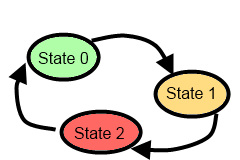
\includegraphics{fsm_traffic_lights.png}
\end{quote}

We're going to build a program that uses a turtle to simulate the traffic lights.
There are three lessons here. The first shows off some different ways to use our turtles.
The second demonstrates how we would program a state machine in Python, by using a variable
to keep track of the current state, and a number of different \code{if} statements to
inspect the current state, and take the actions as we change to a different state.
The third lesson is to use events from the keyboard to trigger the state changes.

Copy and run this program.  Make sure you understand what each line does, consulting the
documentation as you need to.

\begin{Verbatim}[commandchars=\\\{\},numbers=left,firstnumber=1,stepnumber=1]
\PYG{k+kn}{import} \PYG{n+nn}{turtle}           \PYG{c}{\PYGZsh{} Tess becomes a traffic light.}

\PYG{n}{turtle}\PYG{o}{.}\PYG{n}{setup}\PYG{p}{(}\PYG{l+m+mi}{400}\PYG{p}{,}\PYG{l+m+mi}{500}\PYG{p}{)}
\PYG{n}{wn} \PYG{o}{=} \PYG{n}{turtle}\PYG{o}{.}\PYG{n}{Screen}\PYG{p}{(}\PYG{p}{)}
\PYG{n}{wn}\PYG{o}{.}\PYG{n}{title}\PYG{p}{(}\PYG{l+s}{"}\PYG{l+s}{Tess becomes a traffic light!}\PYG{l+s}{"}\PYG{p}{)}
\PYG{n}{wn}\PYG{o}{.}\PYG{n}{bgcolor}\PYG{p}{(}\PYG{l+s}{"}\PYG{l+s}{lightgreen}\PYG{l+s}{"}\PYG{p}{)}
\PYG{n}{tess} \PYG{o}{=} \PYG{n}{turtle}\PYG{o}{.}\PYG{n}{Turtle}\PYG{p}{(}\PYG{p}{)}


\PYG{k}{def} \PYG{n+nf}{draw\PYGZus{}housing}\PYG{p}{(}\PYG{p}{)}\PYG{p}{:}
    \PYG{l+s+sd}{""" Draw a nice housing to hold the traffic lights """}
    \PYG{n}{tess}\PYG{o}{.}\PYG{n}{pensize}\PYG{p}{(}\PYG{l+m+mi}{3}\PYG{p}{)}
    \PYG{n}{tess}\PYG{o}{.}\PYG{n}{color}\PYG{p}{(}\PYG{l+s}{"}\PYG{l+s}{black}\PYG{l+s}{"}\PYG{p}{,} \PYG{l+s}{"}\PYG{l+s}{darkgrey}\PYG{l+s}{"}\PYG{p}{)}
    \PYG{n}{tess}\PYG{o}{.}\PYG{n}{begin\PYGZus{}fill}\PYG{p}{(}\PYG{p}{)}
    \PYG{n}{tess}\PYG{o}{.}\PYG{n}{forward}\PYG{p}{(}\PYG{l+m+mi}{80}\PYG{p}{)}
    \PYG{n}{tess}\PYG{o}{.}\PYG{n}{left}\PYG{p}{(}\PYG{l+m+mi}{90}\PYG{p}{)}
    \PYG{n}{tess}\PYG{o}{.}\PYG{n}{forward}\PYG{p}{(}\PYG{l+m+mi}{200}\PYG{p}{)}
    \PYG{n}{tess}\PYG{o}{.}\PYG{n}{circle}\PYG{p}{(}\PYG{l+m+mi}{40}\PYG{p}{,} \PYG{l+m+mi}{180}\PYG{p}{)}
    \PYG{n}{tess}\PYG{o}{.}\PYG{n}{forward}\PYG{p}{(}\PYG{l+m+mi}{200}\PYG{p}{)}
    \PYG{n}{tess}\PYG{o}{.}\PYG{n}{left}\PYG{p}{(}\PYG{l+m+mi}{90}\PYG{p}{)}
    \PYG{n}{tess}\PYG{o}{.}\PYG{n}{end\PYGZus{}fill}\PYG{p}{(}\PYG{p}{)}


\PYG{n}{draw\PYGZus{}housing}\PYG{p}{(}\PYG{p}{)}

\PYG{n}{tess}\PYG{o}{.}\PYG{n}{penup}\PYG{p}{(}\PYG{p}{)}
\PYG{c}{\PYGZsh{} Position tess onto the place where the green light should be}
\PYG{n}{tess}\PYG{o}{.}\PYG{n}{forward}\PYG{p}{(}\PYG{l+m+mi}{40}\PYG{p}{)}
\PYG{n}{tess}\PYG{o}{.}\PYG{n}{left}\PYG{p}{(}\PYG{l+m+mi}{90}\PYG{p}{)}
\PYG{n}{tess}\PYG{o}{.}\PYG{n}{forward}\PYG{p}{(}\PYG{l+m+mi}{50}\PYG{p}{)}
\PYG{c}{\PYGZsh{} Turn tess into a big green circle}
\PYG{n}{tess}\PYG{o}{.}\PYG{n}{shape}\PYG{p}{(}\PYG{l+s}{"}\PYG{l+s}{circle}\PYG{l+s}{"}\PYG{p}{)}
\PYG{n}{tess}\PYG{o}{.}\PYG{n}{shapesize}\PYG{p}{(}\PYG{l+m+mi}{3}\PYG{p}{)}
\PYG{n}{tess}\PYG{o}{.}\PYG{n}{fillcolor}\PYG{p}{(}\PYG{l+s}{"}\PYG{l+s}{green}\PYG{l+s}{"}\PYG{p}{)}

\PYG{c}{\PYGZsh{} A traffic light is a kind of state machine with three states,}
\PYG{c}{\PYGZsh{} Green, Orange, Red.  We number these states  0, 1, 2}
\PYG{c}{\PYGZsh{} When the machine changes state, we change tess' position and}
\PYG{c}{\PYGZsh{} her fillcolor.}

\PYG{c}{\PYGZsh{} This variable holds the current state of the machine}
\PYG{n}{state\PYGZus{}num} \PYG{o}{=} \PYG{l+m+mi}{0}


\PYG{k}{def} \PYG{n+nf}{advance\PYGZus{}state\PYGZus{}machine}\PYG{p}{(}\PYG{p}{)}\PYG{p}{:}
    \PYG{k}{global} \PYG{n}{state\PYGZus{}num}
    \PYG{k}{if} \PYG{n}{state\PYGZus{}num} \PYG{o}{==} \PYG{l+m+mi}{0}\PYG{p}{:}       \PYG{c}{\PYGZsh{} Transition from state 0 to state 1}
        \PYG{n}{tess}\PYG{o}{.}\PYG{n}{forward}\PYG{p}{(}\PYG{l+m+mi}{70}\PYG{p}{)}
        \PYG{n}{tess}\PYG{o}{.}\PYG{n}{fillcolor}\PYG{p}{(}\PYG{l+s}{"}\PYG{l+s}{orange}\PYG{l+s}{"}\PYG{p}{)}
        \PYG{n}{state\PYGZus{}num} \PYG{o}{=} \PYG{l+m+mi}{1}
    \PYG{k}{elif} \PYG{n}{state\PYGZus{}num} \PYG{o}{==} \PYG{l+m+mi}{1}\PYG{p}{:}     \PYG{c}{\PYGZsh{} Transition from state 1 to state 2}
        \PYG{n}{tess}\PYG{o}{.}\PYG{n}{forward}\PYG{p}{(}\PYG{l+m+mi}{70}\PYG{p}{)}
        \PYG{n}{tess}\PYG{o}{.}\PYG{n}{fillcolor}\PYG{p}{(}\PYG{l+s}{"}\PYG{l+s}{red}\PYG{l+s}{"}\PYG{p}{)}
        \PYG{n}{state\PYGZus{}num} \PYG{o}{=} \PYG{l+m+mi}{2}
    \PYG{k}{else}\PYG{p}{:}                    \PYG{c}{\PYGZsh{} Transition from state 2 to state 0}
        \PYG{n}{tess}\PYG{o}{.}\PYG{n}{back}\PYG{p}{(}\PYG{l+m+mi}{140}\PYG{p}{)}
        \PYG{n}{tess}\PYG{o}{.}\PYG{n}{fillcolor}\PYG{p}{(}\PYG{l+s}{"}\PYG{l+s}{green}\PYG{l+s}{"}\PYG{p}{)}
        \PYG{n}{state\PYGZus{}num} \PYG{o}{=} \PYG{l+m+mi}{0}

\PYG{c}{\PYGZsh{} Bind the event handler to the space key.}
\PYG{n}{wn}\PYG{o}{.}\PYG{n}{onkey}\PYG{p}{(}\PYG{n}{advance\PYGZus{}state\PYGZus{}machine}\PYG{p}{,} \PYG{l+s}{"}\PYG{l+s}{space}\PYG{l+s}{"}\PYG{p}{)}

\PYG{n}{wn}\PYG{o}{.}\PYG{n}{listen}\PYG{p}{(}\PYG{p}{)}                      \PYG{c}{\PYGZsh{} Listen for events}
\PYG{n}{wn}\PYG{o}{.}\PYG{n}{mainloop}\PYG{p}{(}\PYG{p}{)}
\end{Verbatim}

The new Python statement is at line 46.  The \code{global} keyword tells Python not to
create a new local variable for \code{state\_num} (in spite of the fact that
the function assigns to this variable at lines 50, 54, and 58).  Instead, in this function,
\code{state\_num} always refers to the variable that was created at line 42.

What the code in \code{advance\_state\_machine} does is advance from whatever
the current state is, to the next state.  On the state change we move tess
to her new position, change her color, and, of course, we assign to \code{state\_num}
the number of the new state we've just entered.

Each time the space bar is pressed, the event handler causes the traffic light
machine to move to its new state.


\section{Glossary}
\label{events:glossary}\begin{description}
\item[{\index{bind|textbf}bind}] \leavevmode\phantomsection\label{events:term-bind}
We bind a function (or associate it) with an event, meaning that when the event occurs, the
function is called to handle it.

\item[{\index{event|textbf}event}] \leavevmode\phantomsection\label{events:term-event}
Something that happens ``outside'' the normal control flow of our program, usually from some user action.
Typical events are mouse operations and keypresses.  We've also seen that a timer can be primed
to create an event.

\item[{\index{handler|textbf}handler}] \leavevmode\phantomsection\label{events:term-handler}
A function that is called in response to an event.

\end{description}


\section{Exercises}
\label{events:exercises}\begin{enumerate}
\item {} 
Add some new key bindings to the first sample program:
\begin{itemize}
\item {} 
Pressing keys R, G or B should change tess' color to Red, Green or Blue.

\item {} 
Pressing keys + or - should increase or decrease the width of tess' pen.
Ensure that the pen size stays between 1 and 20 (inclusive).

\item {} 
Handle some other keys to change some attributes of tess, or attributes of the window,
or to give her new behaviour that can be controlled from the keyboard.

\end{itemize}

\item {} 
Change the traffic light program so that changes occur automatically, driven by a timer.

\item {} 
In an earlier chapter we saw two turtle methods, \code{hideturtle} and \code{showturtle} that
can hide or show a turtle.  This suggests that we could take a different approach to
the traffic lights program.  Modify the program so that we create three separate
turtles for each of the green, orange and red lights, and instead of moving tess to
different positions and changing her color, we just make one of the three turtles visible
at any time. Once you've made the changes, sit back and ponder some deep thoughts: you've
got two programs, both seem to do the same thing. Is one approach somehow preferable to
the other?  Which one more closely resembles reality --- i.e. the traffic lights in your town?

\item {} 
Now that you've got a traffic light program with different turtles for each light, perhaps
the visibility / invisibility trick wasn't such a great idea. If we watch the traffic lights, they
turn on and off --- but when they're off they are still there, perhaps just a darker color.
Modify the program now so that the lights don't disappear: they are either on, or off. But when
they're off, they're still visible.

\item {} 
Your traffic light controller program has been patented, and you're about to
become seriously rich.  But your new client needs a change.  They want
four states in their state machine: Green, then Green and Orange together,
then Orange only, and then Red.  Additionally, they want different
times spent in each state.  The machine should spend 3 seconds in the Green state,
followed by one second in the Green+Orange state, then one second in
the Orange state, and then 2 seconds in the Red state.
Change the logic in the state machine.

\item {} 
If you don't know how tennis scoring works, ask a friend or consult Wikipedia.  A single
game in tennis between player A and player B always has a score.  We want to think
about the ``state of the score'' as a state machine.   The game starts in state (0, 0), meaning
neither player has any score yet.  We'll assume the first element in this pair is the score
for player A.   If player A wins the first point, the score becomes (15, 0).
If B wins the first point, the state becomes (0, 15).  Below are the first
few states and transitions for a state diagram. In this diagram, each state
has two possible outcomes (A wins the next point, or B does), and the
uppermost arrow is always the transition that happens when A wins the point.
Complete the diagram, showing all transitions and all states.
(Hint: there are twenty states, if you include the duece state, the advantage states,
and the ``A wins'' and ``B wins'' states in your diagram.)

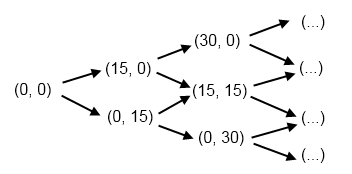
\includegraphics{fsm_tennis_scores.png}

\end{enumerate}

\index{list}\index{element}\index{item}\index{sequence}\index{collection}

\chapter{Lists}
\label{lists:index-0}\label{lists::doc}\label{lists:lists}
A \textbf{list} is an ordered collection of values. The values that make up a list
are called its \textbf{elements}, or its \textbf{items}.
We will use the term \emph{element} or \emph{item} to mean the same thing. Lists are
similar to strings, which are ordered collections of characters, except that the
elements of a list can be of any type.  Lists and strings --- and other collections
that maintain the order of their items --- are called \textbf{sequences}.

\index{nested list}\index{list!nested}

\section{List values}
\label{lists:list-values}\label{lists:index-1}
There are several ways to create a new list; the simplest is to enclose the
elements in square brackets (\code{{[}} and \code{{]}}):
\begin{quote}

\begin{Verbatim}[commandchars=\\\{\},numbers=left,firstnumber=1,stepnumber=1]
\PYG{n}{ps} \PYG{o}{=} \PYG{p}{[}\PYG{l+m+mi}{10}\PYG{p}{,} \PYG{l+m+mi}{20}\PYG{p}{,} \PYG{l+m+mi}{30}\PYG{p}{,} \PYG{l+m+mi}{40}\PYG{p}{]}
\PYG{n}{qs} \PYG{o}{=} \PYG{p}{[}\PYG{l+s}{"}\PYG{l+s}{spam}\PYG{l+s}{"}\PYG{p}{,} \PYG{l+s}{"}\PYG{l+s}{bungee}\PYG{l+s}{"}\PYG{p}{,} \PYG{l+s}{"}\PYG{l+s}{swallow}\PYG{l+s}{"}\PYG{p}{]}
\end{Verbatim}
\end{quote}

The first example is a list of four integers. The second is a list of three
strings. The elements of a list don't have to be the same type.  The following
list contains a string, a float, an integer, and
(amazingly) another list:
\begin{quote}

\begin{Verbatim}[commandchars=\\\{\},numbers=left,firstnumber=1,stepnumber=1]
\PYG{n}{zs} \PYG{o}{=} \PYG{p}{[}\PYG{l+s}{"}\PYG{l+s}{hello}\PYG{l+s}{"}\PYG{p}{,} \PYG{l+m+mf}{2.0}\PYG{p}{,} \PYG{l+m+mi}{5}\PYG{p}{,} \PYG{p}{[}\PYG{l+m+mi}{10}\PYG{p}{,} \PYG{l+m+mi}{20}\PYG{p}{]}\PYG{p}{]}
\end{Verbatim}
\end{quote}

A list within another list is said to be \textbf{nested}.

Finally, a list with no elements is called an empty list,
and is denoted \code{{[}{]}}.

We have already seen that we can assign list values to variables or pass lists as parameters to functions:
\begin{quote}

\begin{Verbatim}[commandchars=\\\{\},numbers=left,firstnumber=1,stepnumber=1]
\PYG{g+gp}{\PYGZgt{}\PYGZgt{}\PYGZgt{} }\PYG{n}{vocabulary} \PYG{o}{=} \PYG{p}{[}\PYG{l+s}{"}\PYG{l+s}{apple}\PYG{l+s}{"}\PYG{p}{,} \PYG{l+s}{"}\PYG{l+s}{cheese}\PYG{l+s}{"}\PYG{p}{,} \PYG{l+s}{"}\PYG{l+s}{dog}\PYG{l+s}{"}\PYG{p}{]}
\PYG{g+gp}{\PYGZgt{}\PYGZgt{}\PYGZgt{} }\PYG{n}{numbers} \PYG{o}{=} \PYG{p}{[}\PYG{l+m+mi}{17}\PYG{p}{,} \PYG{l+m+mi}{123}\PYG{p}{]}
\PYG{g+gp}{\PYGZgt{}\PYGZgt{}\PYGZgt{} }\PYG{n}{an\PYGZus{}empty\PYGZus{}list} \PYG{o}{=} \PYG{p}{[}\PYG{p}{]}
\PYG{g+gp}{\PYGZgt{}\PYGZgt{}\PYGZgt{} }\PYG{n+nb}{print}\PYG{p}{(}\PYG{n}{vocabulary}\PYG{p}{,} \PYG{n}{numbers}\PYG{p}{,} \PYG{n}{an\PYGZus{}empty\PYGZus{}list}\PYG{p}{)}
\PYG{g+go}{["apple", "cheese", "dog"] [17, 123] []}
\end{Verbatim}
\end{quote}
\phantomsection\label{lists:accessing-elements}
\index{list index}\index{index}\index{list traversal}

\section{Accessing elements}
\label{lists:index-2}\label{lists:id1}
The syntax for accessing the elements of a list is the same as the syntax for
accessing the characters of a string --- the index operator: \code{{[}{]}} (not to
be confused with an empty list). The expression inside the brackets specifies
the index. Remember that the indices start at 0:
\begin{quote}

\begin{Verbatim}[commandchars=\\\{\}]
\PYG{g+gp}{\PYGZgt{}\PYGZgt{}\PYGZgt{} }\PYG{n}{numbers}\PYG{p}{[}\PYG{l+m+mi}{0}\PYG{p}{]}
\PYG{g+go}{17}
\end{Verbatim}
\end{quote}

Any expression evaluating to an integer can be used as an index:
\begin{quote}

\begin{Verbatim}[commandchars=\\\{\}]
\PYG{g+gp}{\PYGZgt{}\PYGZgt{}\PYGZgt{} }\PYG{n}{numbers}\PYG{p}{[}\PYG{l+m+mi}{9}\PYG{o}{-}\PYG{l+m+mi}{8}\PYG{p}{]}
\PYG{g+go}{5}
\PYG{g+gp}{\PYGZgt{}\PYGZgt{}\PYGZgt{} }\PYG{n}{numbers}\PYG{p}{[}\PYG{l+m+mf}{1.0}\PYG{p}{]}
\PYG{g+gt}{Traceback (most recent call last):}
  File \PYG{n+nb}{"\PYGZlt{}interactive input\PYGZgt{}"}, line \PYG{l+m}{1}, in \PYG{n}{\PYGZlt{}module\PYGZgt{}}
\PYG{g+gr}{TypeError}: \PYG{n}{list indices must be integers, not float}
\end{Verbatim}
\end{quote}

If you try to access or assign to an element that does not exist, you get a runtime
error:
\begin{quote}

\begin{Verbatim}[commandchars=\\\{\}]
\PYG{g+gp}{\PYGZgt{}\PYGZgt{}\PYGZgt{} }\PYG{n}{numbers}\PYG{p}{[}\PYG{l+m+mi}{2}\PYG{p}{]}
\PYG{g+gt}{Traceback (most recent call last):}
  File \PYG{n+nb}{"\PYGZlt{}interactive input\PYGZgt{}"}, line \PYG{l+m}{1}, in \PYG{n}{\PYGZlt{}module\PYGZgt{}}
\PYG{g+gr}{IndexError}: \PYG{n}{list index out of range}
\end{Verbatim}
\end{quote}

It is common to use a loop variable as a list index.
\begin{quote}

\begin{Verbatim}[commandchars=\\\{\},numbers=left,firstnumber=1,stepnumber=1]
\PYG{n}{horsemen} \PYG{o}{=} \PYG{p}{[}\PYG{l+s}{"}\PYG{l+s}{war}\PYG{l+s}{"}\PYG{p}{,} \PYG{l+s}{"}\PYG{l+s}{famine}\PYG{l+s}{"}\PYG{p}{,} \PYG{l+s}{"}\PYG{l+s}{pestilence}\PYG{l+s}{"}\PYG{p}{,} \PYG{l+s}{"}\PYG{l+s}{death}\PYG{l+s}{"}\PYG{p}{]}

\PYG{k}{for} \PYG{n}{i} \PYG{o+ow}{in} \PYG{p}{[}\PYG{l+m+mi}{0}\PYG{p}{,} \PYG{l+m+mi}{1}\PYG{p}{,} \PYG{l+m+mi}{2}\PYG{p}{,} \PYG{l+m+mi}{3}\PYG{p}{]}\PYG{p}{:}
    \PYG{n+nb}{print}\PYG{p}{(}\PYG{n}{horsemen}\PYG{p}{[}\PYG{n}{i}\PYG{p}{]}\PYG{p}{)}
\end{Verbatim}
\end{quote}

Each time through the loop, the variable \code{i} is used as an index into the
list, printing the \code{i}`th element. This pattern of computation is called a
\textbf{list traversal}.

The above sample doesn't need or use the index \code{i} for anything besides getting
the items from the list, so this more direct version --- where the \code{for} loop gets
the items --- might be preferred:
\begin{quote}

\begin{Verbatim}[commandchars=\\\{\},numbers=left,firstnumber=1,stepnumber=1]
\PYG{n}{horsemen} \PYG{o}{=} \PYG{p}{[}\PYG{l+s}{"}\PYG{l+s}{war}\PYG{l+s}{"}\PYG{p}{,} \PYG{l+s}{"}\PYG{l+s}{famine}\PYG{l+s}{"}\PYG{p}{,} \PYG{l+s}{"}\PYG{l+s}{pestilence}\PYG{l+s}{"}\PYG{p}{,} \PYG{l+s}{"}\PYG{l+s}{death}\PYG{l+s}{"}\PYG{p}{]}

\PYG{k}{for} \PYG{n}{h} \PYG{o+ow}{in} \PYG{n}{horsemen}\PYG{p}{:}
    \PYG{n+nb}{print}\PYG{p}{(}\PYG{n}{h}\PYG{p}{)}
\end{Verbatim}
\end{quote}


\section{List length}
\label{lists:list-length}
The function \code{len} returns the length of a list, which is equal to the number
of its elements. If you are going to use an integer index to access the list,
it is a good idea to use this value as the upper bound of a
loop instead of a constant. That way, if the size of the list changes, you
won't have to go through the program changing all the loops; they will work
correctly for any size list:
\begin{quote}

\begin{Verbatim}[commandchars=\\\{\},numbers=left,firstnumber=1,stepnumber=1]
\PYG{n}{horsemen} \PYG{o}{=} \PYG{p}{[}\PYG{l+s}{"}\PYG{l+s}{war}\PYG{l+s}{"}\PYG{p}{,} \PYG{l+s}{"}\PYG{l+s}{famine}\PYG{l+s}{"}\PYG{p}{,} \PYG{l+s}{"}\PYG{l+s}{pestilence}\PYG{l+s}{"}\PYG{p}{,} \PYG{l+s}{"}\PYG{l+s}{death}\PYG{l+s}{"}\PYG{p}{]}

\PYG{k}{for} \PYG{n}{i} \PYG{o+ow}{in} \PYG{n+nb}{range}\PYG{p}{(}\PYG{n+nb}{len}\PYG{p}{(}\PYG{n}{horsemen}\PYG{p}{)}\PYG{p}{)}\PYG{p}{:}
    \PYG{n+nb}{print}\PYG{p}{(}\PYG{n}{horsemen}\PYG{p}{[}\PYG{n}{i}\PYG{p}{]}\PYG{p}{)}
\end{Verbatim}
\end{quote}

The last time the body of the loop is executed, \code{i} is \code{len(horsemen) - 1},
which is the index of the last element. (But the version without the index
looks even better now!)

Although a list can contain another list, the nested list still counts as a
single element in its parent list. The length of this list is 4:
\begin{quote}

\begin{Verbatim}[commandchars=\\\{\}]
\PYG{g+gp}{\PYGZgt{}\PYGZgt{}\PYGZgt{} }\PYG{n+nb}{len}\PYG{p}{(}\PYG{p}{[}\PYG{l+s}{"}\PYG{l+s}{car makers}\PYG{l+s}{"}\PYG{p}{,} \PYG{l+m+mi}{1}\PYG{p}{,} \PYG{p}{[}\PYG{l+s}{"}\PYG{l+s}{Ford}\PYG{l+s}{"}\PYG{p}{,} \PYG{l+s}{"}\PYG{l+s}{Toyota}\PYG{l+s}{"}\PYG{p}{,} \PYG{l+s}{"}\PYG{l+s}{BMW}\PYG{l+s}{"}\PYG{p}{]}\PYG{p}{,} \PYG{p}{[}\PYG{l+m+mi}{1}\PYG{p}{,} \PYG{l+m+mi}{2}\PYG{p}{,} \PYG{l+m+mi}{3}\PYG{p}{]}\PYG{p}{]}\PYG{p}{)}
\PYG{g+go}{4}
\end{Verbatim}
\end{quote}


\section{List membership}
\label{lists:list-membership}
\code{in} and \code{not in} are Boolean operators that test membership in a sequence. We
used them previously with strings, but they also work with lists and
other sequences:
\begin{quote}

\begin{Verbatim}[commandchars=\\\{\}]
\PYG{g+gp}{\PYGZgt{}\PYGZgt{}\PYGZgt{} }\PYG{n}{horsemen} \PYG{o}{=} \PYG{p}{[}\PYG{l+s}{"}\PYG{l+s}{war}\PYG{l+s}{"}\PYG{p}{,} \PYG{l+s}{"}\PYG{l+s}{famine}\PYG{l+s}{"}\PYG{p}{,} \PYG{l+s}{"}\PYG{l+s}{pestilence}\PYG{l+s}{"}\PYG{p}{,} \PYG{l+s}{"}\PYG{l+s}{death}\PYG{l+s}{"}\PYG{p}{]}
\PYG{g+gp}{\PYGZgt{}\PYGZgt{}\PYGZgt{} }\PYG{l+s}{"}\PYG{l+s}{pestilence}\PYG{l+s}{"} \PYG{o+ow}{in} \PYG{n}{horsemen}
\PYG{g+go}{True}
\PYG{g+gp}{\PYGZgt{}\PYGZgt{}\PYGZgt{} }\PYG{l+s}{"}\PYG{l+s}{debauchery}\PYG{l+s}{"} \PYG{o+ow}{in} \PYG{n}{horsemen}
\PYG{g+go}{False}
\PYG{g+gp}{\PYGZgt{}\PYGZgt{}\PYGZgt{} }\PYG{l+s}{"}\PYG{l+s}{debauchery}\PYG{l+s}{"} \PYG{o+ow}{not} \PYG{o+ow}{in} \PYG{n}{horsemen}
\PYG{g+go}{True}
\end{Verbatim}
\end{quote}

Using this produces a more elegant version of the nested loop program we previously used
to count the number of students doing Computer Science
in the section {\hyperref[iteration:nested-data]{\emph{Nested Loops for Nested Data}}}:
\begin{quote}

\begin{Verbatim}[commandchars=\\\{\},numbers=left,firstnumber=1,stepnumber=1]
\PYG{n}{students} \PYG{o}{=} \PYG{p}{[}
    \PYG{p}{(}\PYG{l+s}{"}\PYG{l+s}{John}\PYG{l+s}{"}\PYG{p}{,} \PYG{p}{[}\PYG{l+s}{"}\PYG{l+s}{CompSci}\PYG{l+s}{"}\PYG{p}{,} \PYG{l+s}{"}\PYG{l+s}{Physics}\PYG{l+s}{"}\PYG{p}{]}\PYG{p}{)}\PYG{p}{,}
    \PYG{p}{(}\PYG{l+s}{"}\PYG{l+s}{Vusi}\PYG{l+s}{"}\PYG{p}{,} \PYG{p}{[}\PYG{l+s}{"}\PYG{l+s}{Maths}\PYG{l+s}{"}\PYG{p}{,} \PYG{l+s}{"}\PYG{l+s}{CompSci}\PYG{l+s}{"}\PYG{p}{,} \PYG{l+s}{"}\PYG{l+s}{Stats}\PYG{l+s}{"}\PYG{p}{]}\PYG{p}{)}\PYG{p}{,}
    \PYG{p}{(}\PYG{l+s}{"}\PYG{l+s}{Jess}\PYG{l+s}{"}\PYG{p}{,} \PYG{p}{[}\PYG{l+s}{"}\PYG{l+s}{CompSci}\PYG{l+s}{"}\PYG{p}{,} \PYG{l+s}{"}\PYG{l+s}{Accounting}\PYG{l+s}{"}\PYG{p}{,} \PYG{l+s}{"}\PYG{l+s}{Economics}\PYG{l+s}{"}\PYG{p}{,} \PYG{l+s}{"}\PYG{l+s}{Management}\PYG{l+s}{"}\PYG{p}{]}\PYG{p}{)}\PYG{p}{,}
    \PYG{p}{(}\PYG{l+s}{"}\PYG{l+s}{Sarah}\PYG{l+s}{"}\PYG{p}{,} \PYG{p}{[}\PYG{l+s}{"}\PYG{l+s}{InfSys}\PYG{l+s}{"}\PYG{p}{,} \PYG{l+s}{"}\PYG{l+s}{Accounting}\PYG{l+s}{"}\PYG{p}{,} \PYG{l+s}{"}\PYG{l+s}{Economics}\PYG{l+s}{"}\PYG{p}{,} \PYG{l+s}{"}\PYG{l+s}{CommLaw}\PYG{l+s}{"}\PYG{p}{]}\PYG{p}{)}\PYG{p}{,}
    \PYG{p}{(}\PYG{l+s}{"}\PYG{l+s}{Zuki}\PYG{l+s}{"}\PYG{p}{,} \PYG{p}{[}\PYG{l+s}{"}\PYG{l+s}{Sociology}\PYG{l+s}{"}\PYG{p}{,} \PYG{l+s}{"}\PYG{l+s}{Economics}\PYG{l+s}{"}\PYG{p}{,} \PYG{l+s}{"}\PYG{l+s}{Law}\PYG{l+s}{"}\PYG{p}{,} \PYG{l+s}{"}\PYG{l+s}{Stats}\PYG{l+s}{"}\PYG{p}{,} \PYG{l+s}{"}\PYG{l+s}{Music}\PYG{l+s}{"}\PYG{p}{]}\PYG{p}{)}\PYG{p}{]}

\PYG{c}{\PYGZsh{} Count how many students are taking CompSci}
\PYG{n}{counter} \PYG{o}{=} \PYG{l+m+mi}{0}
\PYG{k}{for} \PYG{p}{(}\PYG{n}{name}\PYG{p}{,} \PYG{n}{subjects}\PYG{p}{)} \PYG{o+ow}{in} \PYG{n}{students}\PYG{p}{:}
    \PYG{k}{if} \PYG{l+s}{"}\PYG{l+s}{CompSci}\PYG{l+s}{"} \PYG{o+ow}{in} \PYG{n}{subjects}\PYG{p}{:}
           \PYG{n}{counter} \PYG{o}{+}\PYG{o}{=} \PYG{l+m+mi}{1}

\PYG{n+nb}{print}\PYG{p}{(}\PYG{l+s}{"}\PYG{l+s}{The number of students taking CompSci is}\PYG{l+s}{"}\PYG{p}{,} \PYG{n}{counter}\PYG{p}{)}
\end{Verbatim}
\end{quote}


\section{List operations}
\label{lists:list-operations}
The \code{+} operator concatenates lists:
\begin{quote}

\begin{Verbatim}[commandchars=\\\{\}]
\PYG{g+gp}{\PYGZgt{}\PYGZgt{}\PYGZgt{} }\PYG{n}{a} \PYG{o}{=} \PYG{p}{[}\PYG{l+m+mi}{1}\PYG{p}{,} \PYG{l+m+mi}{2}\PYG{p}{,} \PYG{l+m+mi}{3}\PYG{p}{]}
\PYG{g+gp}{\PYGZgt{}\PYGZgt{}\PYGZgt{} }\PYG{n}{b} \PYG{o}{=} \PYG{p}{[}\PYG{l+m+mi}{4}\PYG{p}{,} \PYG{l+m+mi}{5}\PYG{p}{,} \PYG{l+m+mi}{6}\PYG{p}{]}
\PYG{g+gp}{\PYGZgt{}\PYGZgt{}\PYGZgt{} }\PYG{n}{c} \PYG{o}{=} \PYG{n}{a} \PYG{o}{+} \PYG{n}{b}
\PYG{g+gp}{\PYGZgt{}\PYGZgt{}\PYGZgt{} }\PYG{n}{c}
\PYG{g+go}{[1, 2, 3, 4, 5, 6]}
\end{Verbatim}
\end{quote}

Similarly, the \code{*} operator repeats a list a given number of times:
\begin{quote}

\begin{Verbatim}[commandchars=\\\{\}]
\PYG{g+gp}{\PYGZgt{}\PYGZgt{}\PYGZgt{} }\PYG{p}{[}\PYG{l+m+mi}{0}\PYG{p}{]} \PYG{o}{*} \PYG{l+m+mi}{4}
\PYG{g+go}{[0, 0, 0, 0]}
\PYG{g+gp}{\PYGZgt{}\PYGZgt{}\PYGZgt{} }\PYG{p}{[}\PYG{l+m+mi}{1}\PYG{p}{,} \PYG{l+m+mi}{2}\PYG{p}{,} \PYG{l+m+mi}{3}\PYG{p}{]} \PYG{o}{*} \PYG{l+m+mi}{3}
\PYG{g+go}{[1, 2, 3, 1, 2, 3, 1, 2, 3]}
\end{Verbatim}
\end{quote}

The first example repeats \code{{[}0{]}} four times. The second example repeats the
list \code{{[}1, 2, 3{]}} three times.

\index{slice}\index{sublist}

\section{List slices}
\label{lists:list-slices}\label{lists:index-3}
The slice operations we saw previously with strings let us work with sublists:
\begin{quote}

\begin{Verbatim}[commandchars=\\\{\}]
\PYG{g+gp}{\PYGZgt{}\PYGZgt{}\PYGZgt{} }\PYG{n}{a\PYGZus{}list} \PYG{o}{=} \PYG{p}{[}\PYG{l+s}{"}\PYG{l+s}{a}\PYG{l+s}{"}\PYG{p}{,} \PYG{l+s}{"}\PYG{l+s}{b}\PYG{l+s}{"}\PYG{p}{,} \PYG{l+s}{"}\PYG{l+s}{c}\PYG{l+s}{"}\PYG{p}{,} \PYG{l+s}{"}\PYG{l+s}{d}\PYG{l+s}{"}\PYG{p}{,} \PYG{l+s}{"}\PYG{l+s}{e}\PYG{l+s}{"}\PYG{p}{,} \PYG{l+s}{"}\PYG{l+s}{f}\PYG{l+s}{"}\PYG{p}{]}
\PYG{g+gp}{\PYGZgt{}\PYGZgt{}\PYGZgt{} }\PYG{n}{a\PYGZus{}list}\PYG{p}{[}\PYG{l+m+mi}{1}\PYG{p}{:}\PYG{l+m+mi}{3}\PYG{p}{]}
\PYG{g+go}{['b', 'c']}
\PYG{g+gp}{\PYGZgt{}\PYGZgt{}\PYGZgt{} }\PYG{n}{a\PYGZus{}list}\PYG{p}{[}\PYG{p}{:}\PYG{l+m+mi}{4}\PYG{p}{]}
\PYG{g+go}{['a', 'b', 'c', 'd']}
\PYG{g+gp}{\PYGZgt{}\PYGZgt{}\PYGZgt{} }\PYG{n}{a\PYGZus{}list}\PYG{p}{[}\PYG{l+m+mi}{3}\PYG{p}{:}\PYG{p}{]}
\PYG{g+go}{['d', 'e', 'f']}
\PYG{g+gp}{\PYGZgt{}\PYGZgt{}\PYGZgt{} }\PYG{n}{a\PYGZus{}list}\PYG{p}{[}\PYG{p}{:}\PYG{p}{]}
\PYG{g+go}{['a', 'b', 'c', 'd', 'e', 'f']}
\end{Verbatim}
\end{quote}

\index{mutable}\index{item assignment}\index{immutable}

\section{Lists are mutable}
\label{lists:index-4}\label{lists:lists-are-mutable}
Unlike strings, lists are \textbf{mutable}, which means we can change their
elements. Using the index operator on the left side of an assignment, we can
update one of the elements:
\begin{quote}

\begin{Verbatim}[commandchars=\\\{\}]
\PYG{g+gp}{\PYGZgt{}\PYGZgt{}\PYGZgt{} }\PYG{n}{fruit} \PYG{o}{=} \PYG{p}{[}\PYG{l+s}{"}\PYG{l+s}{banana}\PYG{l+s}{"}\PYG{p}{,} \PYG{l+s}{"}\PYG{l+s}{apple}\PYG{l+s}{"}\PYG{p}{,} \PYG{l+s}{"}\PYG{l+s}{quince}\PYG{l+s}{"}\PYG{p}{]}
\PYG{g+gp}{\PYGZgt{}\PYGZgt{}\PYGZgt{} }\PYG{n}{fruit}\PYG{p}{[}\PYG{l+m+mi}{0}\PYG{p}{]} \PYG{o}{=} \PYG{l+s}{"}\PYG{l+s}{pear}\PYG{l+s}{"}
\PYG{g+gp}{\PYGZgt{}\PYGZgt{}\PYGZgt{} }\PYG{n}{fruit}\PYG{p}{[}\PYG{l+m+mi}{2}\PYG{p}{]} \PYG{o}{=} \PYG{l+s}{"}\PYG{l+s}{orange}\PYG{l+s}{"}
\PYG{g+gp}{\PYGZgt{}\PYGZgt{}\PYGZgt{} }\PYG{n}{fruit}
\PYG{g+go}{['pear', 'apple', 'orange']}
\end{Verbatim}
\end{quote}

The bracket operator applied to a list can appear anywhere in an expression.
When it appears on the left side of an assignment, it changes one of the
elements in the list, so the first element of \code{fruit} has been changed from
\code{"banana"} to \code{"pear"}, and the last from \code{"quince"} to \code{"orange"}. An
assignment to an element of a list is called \textbf{item assignment}. Item
assignment does not work for strings:
\begin{quote}

\begin{Verbatim}[commandchars=\\\{\}]
\PYG{g+gp}{\PYGZgt{}\PYGZgt{}\PYGZgt{} }\PYG{n}{my\PYGZus{}string} \PYG{o}{=} \PYG{l+s}{"}\PYG{l+s}{TEST}\PYG{l+s}{"}
\PYG{g+gp}{\PYGZgt{}\PYGZgt{}\PYGZgt{} }\PYG{n}{my\PYGZus{}string}\PYG{p}{[}\PYG{l+m+mi}{2}\PYG{p}{]} \PYG{o}{=} \PYG{l+s}{"}\PYG{l+s}{X}\PYG{l+s}{"}
\PYG{g+gt}{Traceback (most recent call last):}
  File \PYG{n+nb}{"\PYGZlt{}interactive input\PYGZgt{}"}, line \PYG{l+m}{1}, in \PYG{n}{\PYGZlt{}module\PYGZgt{}}
\PYG{g+gr}{TypeError}: \PYG{n}{'str' object does not support item assignment}
\end{Verbatim}
\end{quote}

but it does for lists:
\begin{quote}

\begin{Verbatim}[commandchars=\\\{\}]
\PYG{g+gp}{\PYGZgt{}\PYGZgt{}\PYGZgt{} }\PYG{n}{my\PYGZus{}list} \PYG{o}{=} \PYG{p}{[}\PYG{l+s}{"}\PYG{l+s}{T}\PYG{l+s}{"}\PYG{p}{,} \PYG{l+s}{"}\PYG{l+s}{E}\PYG{l+s}{"}\PYG{p}{,} \PYG{l+s}{"}\PYG{l+s}{S}\PYG{l+s}{"}\PYG{p}{,} \PYG{l+s}{"}\PYG{l+s}{T}\PYG{l+s}{"}\PYG{p}{]}
\PYG{g+gp}{\PYGZgt{}\PYGZgt{}\PYGZgt{} }\PYG{n}{my\PYGZus{}list}\PYG{p}{[}\PYG{l+m+mi}{2}\PYG{p}{]} \PYG{o}{=} \PYG{l+s}{"}\PYG{l+s}{X}\PYG{l+s}{"}
\PYG{g+gp}{\PYGZgt{}\PYGZgt{}\PYGZgt{} }\PYG{n}{my\PYGZus{}list}
\PYG{g+go}{['T', 'E', 'X', 'T']}
\end{Verbatim}
\end{quote}

With the slice operator we can update a whole sublist at once:
\begin{quote}

\begin{Verbatim}[commandchars=\\\{\}]
\PYG{g+gp}{\PYGZgt{}\PYGZgt{}\PYGZgt{} }\PYG{n}{a\PYGZus{}list} \PYG{o}{=} \PYG{p}{[}\PYG{l+s}{"}\PYG{l+s}{a}\PYG{l+s}{"}\PYG{p}{,} \PYG{l+s}{"}\PYG{l+s}{b}\PYG{l+s}{"}\PYG{p}{,} \PYG{l+s}{"}\PYG{l+s}{c}\PYG{l+s}{"}\PYG{p}{,} \PYG{l+s}{"}\PYG{l+s}{d}\PYG{l+s}{"}\PYG{p}{,} \PYG{l+s}{"}\PYG{l+s}{e}\PYG{l+s}{"}\PYG{p}{,} \PYG{l+s}{"}\PYG{l+s}{f}\PYG{l+s}{"}\PYG{p}{]}
\PYG{g+gp}{\PYGZgt{}\PYGZgt{}\PYGZgt{} }\PYG{n}{a\PYGZus{}list}\PYG{p}{[}\PYG{l+m+mi}{1}\PYG{p}{:}\PYG{l+m+mi}{3}\PYG{p}{]} \PYG{o}{=} \PYG{p}{[}\PYG{l+s}{"}\PYG{l+s}{x}\PYG{l+s}{"}\PYG{p}{,} \PYG{l+s}{"}\PYG{l+s}{y}\PYG{l+s}{"}\PYG{p}{]}
\PYG{g+gp}{\PYGZgt{}\PYGZgt{}\PYGZgt{} }\PYG{n}{a\PYGZus{}list}
\PYG{g+go}{['a', 'x', 'y', 'd', 'e', 'f']}
\end{Verbatim}
\end{quote}

We can also remove elements from a list by assigning an empty list to them:
\begin{quote}

\begin{Verbatim}[commandchars=\\\{\}]
\PYG{g+gp}{\PYGZgt{}\PYGZgt{}\PYGZgt{} }\PYG{n}{a\PYGZus{}list} \PYG{o}{=} \PYG{p}{[}\PYG{l+s}{"}\PYG{l+s}{a}\PYG{l+s}{"}\PYG{p}{,} \PYG{l+s}{"}\PYG{l+s}{b}\PYG{l+s}{"}\PYG{p}{,} \PYG{l+s}{"}\PYG{l+s}{c}\PYG{l+s}{"}\PYG{p}{,} \PYG{l+s}{"}\PYG{l+s}{d}\PYG{l+s}{"}\PYG{p}{,} \PYG{l+s}{"}\PYG{l+s}{e}\PYG{l+s}{"}\PYG{p}{,} \PYG{l+s}{"}\PYG{l+s}{f}\PYG{l+s}{"}\PYG{p}{]}
\PYG{g+gp}{\PYGZgt{}\PYGZgt{}\PYGZgt{} }\PYG{n}{a\PYGZus{}list}\PYG{p}{[}\PYG{l+m+mi}{1}\PYG{p}{:}\PYG{l+m+mi}{3}\PYG{p}{]} \PYG{o}{=} \PYG{p}{[}\PYG{p}{]}
\PYG{g+gp}{\PYGZgt{}\PYGZgt{}\PYGZgt{} }\PYG{n}{a\PYGZus{}list}
\PYG{g+go}{['a', 'd', 'e', 'f']}
\end{Verbatim}
\end{quote}

And we can add elements to a list by squeezing them into an empty slice at the
desired location:
\begin{quote}

\begin{Verbatim}[commandchars=\\\{\}]
\PYG{g+gp}{\PYGZgt{}\PYGZgt{}\PYGZgt{} }\PYG{n}{a\PYGZus{}list} \PYG{o}{=} \PYG{p}{[}\PYG{l+s}{"}\PYG{l+s}{a}\PYG{l+s}{"}\PYG{p}{,} \PYG{l+s}{"}\PYG{l+s}{d}\PYG{l+s}{"}\PYG{p}{,} \PYG{l+s}{"}\PYG{l+s}{f}\PYG{l+s}{"}\PYG{p}{]}
\PYG{g+gp}{\PYGZgt{}\PYGZgt{}\PYGZgt{} }\PYG{n}{a\PYGZus{}list}\PYG{p}{[}\PYG{l+m+mi}{1}\PYG{p}{:}\PYG{l+m+mi}{1}\PYG{p}{]} \PYG{o}{=} \PYG{p}{[}\PYG{l+s}{"}\PYG{l+s}{b}\PYG{l+s}{"}\PYG{p}{,} \PYG{l+s}{"}\PYG{l+s}{c}\PYG{l+s}{"}\PYG{p}{]}
\PYG{g+gp}{\PYGZgt{}\PYGZgt{}\PYGZgt{} }\PYG{n}{a\PYGZus{}list}
\PYG{g+go}{['a', 'b', 'c', 'd', 'f']}
\PYG{g+gp}{\PYGZgt{}\PYGZgt{}\PYGZgt{} }\PYG{n}{a\PYGZus{}list}\PYG{p}{[}\PYG{l+m+mi}{4}\PYG{p}{:}\PYG{l+m+mi}{4}\PYG{p}{]} \PYG{o}{=} \PYG{p}{[}\PYG{l+s}{"}\PYG{l+s}{e}\PYG{l+s}{"}\PYG{p}{]}
\PYG{g+gp}{\PYGZgt{}\PYGZgt{}\PYGZgt{} }\PYG{n}{a\PYGZus{}list}
\PYG{g+go}{['a', 'b', 'c', 'd', 'e', 'f']}
\end{Verbatim}
\end{quote}

\index{del statement}\index{statement!del}

\section{List deletion}
\label{lists:index-5}\label{lists:list-deletion}
Using slices to delete list elements can be error-prone.
Python provides an alternative that is more readable.
The \code{del} statement removes an element from a list:
\begin{quote}

\begin{Verbatim}[commandchars=\\\{\}]
\PYG{g+gp}{\PYGZgt{}\PYGZgt{}\PYGZgt{} }\PYG{n}{a} \PYG{o}{=} \PYG{p}{[}\PYG{l+s}{"}\PYG{l+s}{one}\PYG{l+s}{"}\PYG{p}{,} \PYG{l+s}{"}\PYG{l+s}{two}\PYG{l+s}{"}\PYG{p}{,} \PYG{l+s}{"}\PYG{l+s}{three}\PYG{l+s}{"}\PYG{p}{]}
\PYG{g+gp}{\PYGZgt{}\PYGZgt{}\PYGZgt{} }\PYG{k}{del} \PYG{n}{a}\PYG{p}{[}\PYG{l+m+mi}{1}\PYG{p}{]}
\PYG{g+gp}{\PYGZgt{}\PYGZgt{}\PYGZgt{} }\PYG{n}{a}
\PYG{g+go}{['one', 'three']}
\end{Verbatim}
\end{quote}

As you might expect, \code{del} causes a runtime
error if the index is out of range.

You can also use \code{del} with a slice to delete a sublist:
\begin{quote}

\begin{Verbatim}[commandchars=\\\{\}]
\PYG{g+gp}{\PYGZgt{}\PYGZgt{}\PYGZgt{} }\PYG{n}{a\PYGZus{}list} \PYG{o}{=} \PYG{p}{[}\PYG{l+s}{"}\PYG{l+s}{a}\PYG{l+s}{"}\PYG{p}{,} \PYG{l+s}{"}\PYG{l+s}{b}\PYG{l+s}{"}\PYG{p}{,} \PYG{l+s}{"}\PYG{l+s}{c}\PYG{l+s}{"}\PYG{p}{,} \PYG{l+s}{"}\PYG{l+s}{d}\PYG{l+s}{"}\PYG{p}{,} \PYG{l+s}{"}\PYG{l+s}{e}\PYG{l+s}{"}\PYG{p}{,} \PYG{l+s}{"}\PYG{l+s}{f}\PYG{l+s}{"}\PYG{p}{]}
\PYG{g+gp}{\PYGZgt{}\PYGZgt{}\PYGZgt{} }\PYG{k}{del} \PYG{n}{a\PYGZus{}list}\PYG{p}{[}\PYG{l+m+mi}{1}\PYG{p}{:}\PYG{l+m+mi}{5}\PYG{p}{]}
\PYG{g+gp}{\PYGZgt{}\PYGZgt{}\PYGZgt{} }\PYG{n}{a\PYGZus{}list}
\PYG{g+go}{['a', 'f']}
\end{Verbatim}
\end{quote}

As usual, the sublist selected by slice contains all the elements up to, but not including, the second
index.

\index{is operator}\index{objects and values}

\section{Objects and references}
\label{lists:index-6}\label{lists:objects-and-references}
After we execute these assignment statements
\begin{quote}

\begin{Verbatim}[commandchars=\\\{\},numbers=left,firstnumber=1,stepnumber=1]
\PYG{n}{a} \PYG{o}{=} \PYG{l+s}{"}\PYG{l+s}{banana}\PYG{l+s}{"}
\PYG{n}{b} \PYG{o}{=} \PYG{l+s}{"}\PYG{l+s}{banana}\PYG{l+s}{"}
\end{Verbatim}
\end{quote}

we know that \code{a} and \code{b} will refer to a string object with the letters
\code{"banana"}. But we don't know yet whether they point to the \emph{same} string object.

There are two possible ways the Python interpreter could arrange its memory:
\begin{quote}

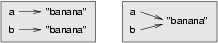
\includegraphics{list1.png}
\end{quote}

In one case, \code{a} and \code{b} refer to two different objects that have the same
value. In the second case, they refer to the same object.

We can test whether two names refer to the same object using the \code{is}
operator:
\begin{quote}

\begin{Verbatim}[commandchars=\\\{\}]
\PYG{g+gp}{\PYGZgt{}\PYGZgt{}\PYGZgt{} }\PYG{n}{a} \PYG{o+ow}{is} \PYG{n}{b}
\PYG{g+go}{True}
\end{Verbatim}
\end{quote}

This tells us that both \code{a} and \code{b} refer to the same object, and that it
is the second of the two state snapshots that accurately describes the relationship.

Since strings are \emph{immutable}, Python optimizes resources by making two names
that refer to the same string value refer to the same object.

This is not the case with lists:
\begin{quote}

\begin{Verbatim}[commandchars=\\\{\}]
\PYG{g+gp}{\PYGZgt{}\PYGZgt{}\PYGZgt{} }\PYG{n}{a} \PYG{o}{=} \PYG{p}{[}\PYG{l+m+mi}{1}\PYG{p}{,} \PYG{l+m+mi}{2}\PYG{p}{,} \PYG{l+m+mi}{3}\PYG{p}{]}
\PYG{g+gp}{\PYGZgt{}\PYGZgt{}\PYGZgt{} }\PYG{n}{b} \PYG{o}{=} \PYG{p}{[}\PYG{l+m+mi}{1}\PYG{p}{,} \PYG{l+m+mi}{2}\PYG{p}{,} \PYG{l+m+mi}{3}\PYG{p}{]}
\PYG{g+gp}{\PYGZgt{}\PYGZgt{}\PYGZgt{} }\PYG{n}{a} \PYG{o}{==} \PYG{n}{b}
\PYG{g+go}{True}
\PYG{g+gp}{\PYGZgt{}\PYGZgt{}\PYGZgt{} }\PYG{n}{a} \PYG{o+ow}{is} \PYG{n}{b}
\PYG{g+go}{False}
\end{Verbatim}
\end{quote}

The state snapshot here looks like this:
\begin{quote}

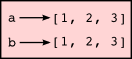
\includegraphics{mult_references2.png}
\end{quote}

\code{a} and \code{b} have the same value but do not refer to the same object.

\index{aliases}

\section{Aliasing}
\label{lists:index-7}\label{lists:aliasing}
Since variables refer to objects, if we assign one variable to another, both
variables refer to the same object:
\begin{quote}

\begin{Verbatim}[commandchars=\\\{\}]
\PYG{g+gp}{\PYGZgt{}\PYGZgt{}\PYGZgt{} }\PYG{n}{a} \PYG{o}{=} \PYG{p}{[}\PYG{l+m+mi}{1}\PYG{p}{,} \PYG{l+m+mi}{2}\PYG{p}{,} \PYG{l+m+mi}{3}\PYG{p}{]}
\PYG{g+gp}{\PYGZgt{}\PYGZgt{}\PYGZgt{} }\PYG{n}{b} \PYG{o}{=} \PYG{n}{a}
\PYG{g+gp}{\PYGZgt{}\PYGZgt{}\PYGZgt{} }\PYG{n}{a} \PYG{o+ow}{is} \PYG{n}{b}
\PYG{g+go}{True}
\end{Verbatim}
\end{quote}

In this case, the state snapshot looks like this:
\begin{quote}

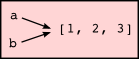
\includegraphics{mult_references3.png}
\end{quote}

Because the same list has two different names, \code{a} and \code{b}, we say that it
is \textbf{aliased}. Changes made with one alias affect the other:
\begin{quote}

\begin{Verbatim}[commandchars=\\\{\}]
\PYG{g+gp}{\PYGZgt{}\PYGZgt{}\PYGZgt{} }\PYG{n}{b}\PYG{p}{[}\PYG{l+m+mi}{0}\PYG{p}{]} \PYG{o}{=} \PYG{l+m+mi}{5}
\PYG{g+gp}{\PYGZgt{}\PYGZgt{}\PYGZgt{} }\PYG{n}{a}
\PYG{g+go}{[5, 2, 3]}
\end{Verbatim}
\end{quote}

Although this behavior can be useful, it is sometimes unexpected or
undesirable. In general, it is safer to avoid aliasing when you are working
with mutable objects (i.e. lists at this point in our textbook,
but we'll meet more mutable objects
as we cover classes and objects, dictionaries and sets).
Of course, for immutable objects (i.e. strings, tuples), there's no problem --- it is
just not possible to change something and get a surprise when you access an alias name.
That's why Python is free to alias strings (and any other immutable kinds of data)
when it sees an opportunity to economize.

\index{clone}

\section{Cloning lists}
\label{lists:cloning-lists}\label{lists:index-8}
If we want to modify a list and also keep a copy of the original, we need to be
able to make a copy of the list itself, not just the reference. This process is
sometimes called \textbf{cloning}, to avoid the ambiguity of the word copy.

The easiest way to clone a list is to use the slice operator:
\begin{quote}

\begin{Verbatim}[commandchars=\\\{\}]
\PYG{g+gp}{\PYGZgt{}\PYGZgt{}\PYGZgt{} }\PYG{n}{a} \PYG{o}{=} \PYG{p}{[}\PYG{l+m+mi}{1}\PYG{p}{,} \PYG{l+m+mi}{2}\PYG{p}{,} \PYG{l+m+mi}{3}\PYG{p}{]}
\PYG{g+gp}{\PYGZgt{}\PYGZgt{}\PYGZgt{} }\PYG{n}{b} \PYG{o}{=} \PYG{n}{a}\PYG{p}{[}\PYG{p}{:}\PYG{p}{]}
\PYG{g+gp}{\PYGZgt{}\PYGZgt{}\PYGZgt{} }\PYG{n}{b}
\PYG{g+go}{[1, 2, 3]}
\end{Verbatim}
\end{quote}

Taking any slice of \code{a} creates a new list. In this case the slice happens to
consist of the whole list.  So now the relationship is like this:
\begin{quote}

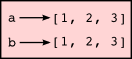
\includegraphics{mult_references2.png}
\end{quote}

Now we are free to make changes to \code{b} without worrying that we'll inadvertently be
changing \code{a}:
\begin{quote}

\begin{Verbatim}[commandchars=\\\{\}]
\PYG{g+gp}{\PYGZgt{}\PYGZgt{}\PYGZgt{} }\PYG{n}{b}\PYG{p}{[}\PYG{l+m+mi}{0}\PYG{p}{]} \PYG{o}{=} \PYG{l+m+mi}{5}
\PYG{g+gp}{\PYGZgt{}\PYGZgt{}\PYGZgt{} }\PYG{n}{a}
\PYG{g+go}{[1, 2, 3]}
\end{Verbatim}
\end{quote}

\index{for loop}\index{enumerate}

\section{Lists and \texttt{for} loops}
\label{lists:lists-and-for-loops}\label{lists:index-9}
The \code{for} loop also works with lists, as we've already seen. The generalized syntax of a \code{for}
loop is:
\begin{quote}

\begin{Verbatim}[commandchars=\\\{\}]
\PYG{k}{for} \PYG{n}{VARIABLE} \PYG{o+ow}{in} \PYG{n}{LIST}\PYG{p}{:}
    \PYG{n}{BODY}
\end{Verbatim}
\end{quote}

So, as we've seen
\begin{quote}

\begin{Verbatim}[commandchars=\\\{\},numbers=left,firstnumber=1,stepnumber=1]
\PYG{n}{friends} \PYG{o}{=} \PYG{p}{[}\PYG{l+s}{"}\PYG{l+s}{Joe}\PYG{l+s}{"}\PYG{p}{,} \PYG{l+s}{"}\PYG{l+s}{Zoe}\PYG{l+s}{"}\PYG{p}{,} \PYG{l+s}{"}\PYG{l+s}{Brad}\PYG{l+s}{"}\PYG{p}{,} \PYG{l+s}{"}\PYG{l+s}{Angelina}\PYG{l+s}{"}\PYG{p}{,} \PYG{l+s}{"}\PYG{l+s}{Zuki}\PYG{l+s}{"}\PYG{p}{,} \PYG{l+s}{"}\PYG{l+s}{Thandi}\PYG{l+s}{"}\PYG{p}{,} \PYG{l+s}{"}\PYG{l+s}{Paris}\PYG{l+s}{"}\PYG{p}{]}
\PYG{k}{for} \PYG{n}{friend} \PYG{o+ow}{in} \PYG{n}{friends}\PYG{p}{:}
    \PYG{n+nb}{print}\PYG{p}{(}\PYG{n}{friend}\PYG{p}{)}
\end{Verbatim}
\end{quote}

It almost reads like English: For (every) friend in (the list of) friends,
print (the name of the) friend.

Any list expression can be used in a \code{for} loop:
\begin{quote}

\begin{Verbatim}[commandchars=\\\{\},numbers=left,firstnumber=1,stepnumber=1]
\PYG{k}{for} \PYG{n}{number} \PYG{o+ow}{in} \PYG{n+nb}{range}\PYG{p}{(}\PYG{l+m+mi}{20}\PYG{p}{)}\PYG{p}{:}
    \PYG{k}{if} \PYG{n}{number} \PYG{o}{\PYGZpc{}} \PYG{l+m+mi}{3} \PYG{o}{==} \PYG{l+m+mi}{0}\PYG{p}{:}
        \PYG{n+nb}{print}\PYG{p}{(}\PYG{n}{number}\PYG{p}{)}

\PYG{k}{for} \PYG{n}{fruit} \PYG{o+ow}{in} \PYG{p}{[}\PYG{l+s}{"}\PYG{l+s}{banana}\PYG{l+s}{"}\PYG{p}{,} \PYG{l+s}{"}\PYG{l+s}{apple}\PYG{l+s}{"}\PYG{p}{,} \PYG{l+s}{"}\PYG{l+s}{quince}\PYG{l+s}{"}\PYG{p}{]}\PYG{p}{:}
    \PYG{n+nb}{print}\PYG{p}{(}\PYG{l+s}{"}\PYG{l+s}{I like to eat }\PYG{l+s}{"} \PYG{o}{+} \PYG{n}{fruit} \PYG{o}{+} \PYG{l+s}{"}\PYG{l+s}{s!}\PYG{l+s}{"}\PYG{p}{)}
\end{Verbatim}
\end{quote}

The first example prints all the multiples of 3 between 0 and 19. The second
example expresses enthusiasm for various fruits.

Since lists are mutable, we often want to traverse a list, changing
each of its elements. The following squares all the numbers in the list \code{xs}:
\begin{quote}

\begin{Verbatim}[commandchars=\\\{\},numbers=left,firstnumber=1,stepnumber=1]
\PYG{n}{xs} \PYG{o}{=} \PYG{p}{[}\PYG{l+m+mi}{1}\PYG{p}{,} \PYG{l+m+mi}{2}\PYG{p}{,} \PYG{l+m+mi}{3}\PYG{p}{,} \PYG{l+m+mi}{4}\PYG{p}{,} \PYG{l+m+mi}{5}\PYG{p}{]}

\PYG{k}{for} \PYG{n}{i} \PYG{o+ow}{in} \PYG{n+nb}{range}\PYG{p}{(}\PYG{n+nb}{len}\PYG{p}{(}\PYG{n}{xs}\PYG{p}{)}\PYG{p}{)}\PYG{p}{:}
    \PYG{n}{xs}\PYG{p}{[}\PYG{n}{i}\PYG{p}{]} \PYG{o}{=} \PYG{n}{xs}\PYG{p}{[}\PYG{n}{i}\PYG{p}{]}\PYG{o}{*}\PYG{o}{*}\PYG{l+m+mi}{2}
\end{Verbatim}
\end{quote}

Take a moment to think about \code{range(len(xs))} until you understand how
it works.

In this example we are interested in both the \emph{value} of an item, (we want to
square that value), and its \emph{index} (so that we can assign the new value to that position).
This pattern is common enough that Python provides a nicer way to implement it:
\begin{quote}

\begin{Verbatim}[commandchars=\\\{\},numbers=left,firstnumber=1,stepnumber=1]
\PYG{n}{xs} \PYG{o}{=} \PYG{p}{[}\PYG{l+m+mi}{1}\PYG{p}{,} \PYG{l+m+mi}{2}\PYG{p}{,} \PYG{l+m+mi}{3}\PYG{p}{,} \PYG{l+m+mi}{4}\PYG{p}{,} \PYG{l+m+mi}{5}\PYG{p}{]}

\PYG{k}{for} \PYG{p}{(}\PYG{n}{i}\PYG{p}{,} \PYG{n}{val}\PYG{p}{)} \PYG{o+ow}{in} \PYG{n+nb}{enumerate}\PYG{p}{(}\PYG{n}{xs}\PYG{p}{)}\PYG{p}{:}
    \PYG{n}{xs}\PYG{p}{[}\PYG{n}{i}\PYG{p}{]} \PYG{o}{=} \PYG{n}{val}\PYG{o}{*}\PYG{o}{*}\PYG{l+m+mi}{2}
\end{Verbatim}
\end{quote}

\code{enumerate} generates pairs of both (index, value) during
the list traversal. Try this next example to see more clearly how \code{enumerate}
works:
\begin{quote}

\begin{Verbatim}[commandchars=\\\{\},numbers=left,firstnumber=1,stepnumber=1]
\PYG{k}{for} \PYG{p}{(}\PYG{n}{i}\PYG{p}{,} \PYG{n}{v}\PYG{p}{)} \PYG{o+ow}{in} \PYG{n+nb}{enumerate}\PYG{p}{(}\PYG{p}{[}\PYG{l+s}{"}\PYG{l+s}{banana}\PYG{l+s}{"}\PYG{p}{,} \PYG{l+s}{"}\PYG{l+s}{apple}\PYG{l+s}{"}\PYG{p}{,} \PYG{l+s}{"}\PYG{l+s}{pear}\PYG{l+s}{"}\PYG{p}{,} \PYG{l+s}{"}\PYG{l+s}{lemon}\PYG{l+s}{"}\PYG{p}{]}\PYG{p}{)}\PYG{p}{:}
     \PYG{n+nb}{print}\PYG{p}{(}\PYG{n}{i}\PYG{p}{,} \PYG{n}{v}\PYG{p}{)}
\end{Verbatim}

\begin{Verbatim}[commandchars=\\\{\}]
\PYG{g+go}{0 banana}
\PYG{g+go}{1 apple}
\PYG{g+go}{2 pear}
\PYG{g+go}{3 lemon}
\end{Verbatim}
\end{quote}

\index{parameter}

\section{List parameters}
\label{lists:list-parameters}\label{lists:index-10}
Passing a list as an argument actually passes a reference to the list, not a
copy or clone of the list. So parameter passing creates an alias for you: the caller
has one variable referencing the list, and the called function has an alias, but there
is only one underlying list object.
For example, the function below takes a list as an
argument and multiplies each element in the list by 2:
\begin{quote}

\begin{Verbatim}[commandchars=\\\{\},numbers=left,firstnumber=1,stepnumber=1]
\PYG{k}{def} \PYG{n+nf}{double\PYGZus{}stuff}\PYG{p}{(}\PYG{n}{a\PYGZus{}list}\PYG{p}{)}\PYG{p}{:}
    \PYG{l+s+sd}{""" Overwrite each element in a\PYGZus{}list with double its value. """}
    \PYG{k}{for} \PYG{p}{(}\PYG{n}{idx}\PYG{p}{,} \PYG{n}{val}\PYG{p}{)} \PYG{o+ow}{in} \PYG{n+nb}{enumerate}\PYG{p}{(}\PYG{n}{a\PYGZus{}list}\PYG{p}{)}\PYG{p}{:}
        \PYG{n}{a\PYGZus{}list}\PYG{p}{[}\PYG{n}{idx}\PYG{p}{]} \PYG{o}{=} \PYG{l+m+mi}{2} \PYG{o}{*} \PYG{n}{val}
\end{Verbatim}
\end{quote}

If we add the following onto our script:
\begin{quote}

\begin{Verbatim}[commandchars=\\\{\},numbers=left,firstnumber=1,stepnumber=1]
\PYG{n}{things} \PYG{o}{=} \PYG{p}{[}\PYG{l+m+mi}{2}\PYG{p}{,} \PYG{l+m+mi}{5}\PYG{p}{,} \PYG{l+m+mi}{9}\PYG{p}{]}
\PYG{n}{double\PYGZus{}stuff}\PYG{p}{(}\PYG{n}{things}\PYG{p}{)}
\PYG{n+nb}{print}\PYG{p}{(}\PYG{n}{things}\PYG{p}{)}
\end{Verbatim}
\end{quote}

When we run it we'll get:
\begin{quote}

\begin{Verbatim}[commandchars=\\\{\}]
\PYG{g+go}{[4, 10, 18]}
\end{Verbatim}
\end{quote}

In the function above, the parameter
\code{a\_list} and the variable \code{things} are aliases for the
same object.  So before any changes to the elements in the list, the state snapshot
looks like this:
\begin{quote}

\includegraphics{mult_references4.png}
\end{quote}

Since the list object is shared by two frames, we drew it between them.

If a function modifies the items of a list parameter, the caller sees the change.
\begin{quote}

\begin{notice}{note}{Use the Python visualizer!}

We've already mentioned the Python visualizer at \href{http://netserv.ict.ru.ac.za/python3\_viz}{http://netserv.ict.ru.ac.za/python3\_viz}.
It is a very useful tool for building a good understanding of references, aliases, assignments,
and passing arguments to functions.  Pay special attention to cases where you clone
a list or have two separate lists, and cases where there is only one underlying list,
but more than one variable is aliased to reference the list.
\end{notice}
\end{quote}

\index{list!append}

\section{List methods}
\label{lists:list-methods}\label{lists:index-11}
The dot operator can also be used to access built-in methods of list objects.  We'll
start with the most useful method for adding something onto the end of an existing list:
\begin{quote}

\begin{Verbatim}[commandchars=\\\{\}]
\PYG{g+gp}{\PYGZgt{}\PYGZgt{}\PYGZgt{} }\PYG{n}{mylist} \PYG{o}{=} \PYG{p}{[}\PYG{p}{]}
\PYG{g+gp}{\PYGZgt{}\PYGZgt{}\PYGZgt{} }\PYG{n}{mylist}\PYG{o}{.}\PYG{n}{append}\PYG{p}{(}\PYG{l+m+mi}{5}\PYG{p}{)}
\PYG{g+gp}{\PYGZgt{}\PYGZgt{}\PYGZgt{} }\PYG{n}{mylist}\PYG{o}{.}\PYG{n}{append}\PYG{p}{(}\PYG{l+m+mi}{27}\PYG{p}{)}
\PYG{g+gp}{\PYGZgt{}\PYGZgt{}\PYGZgt{} }\PYG{n}{mylist}\PYG{o}{.}\PYG{n}{append}\PYG{p}{(}\PYG{l+m+mi}{3}\PYG{p}{)}
\PYG{g+gp}{\PYGZgt{}\PYGZgt{}\PYGZgt{} }\PYG{n}{mylist}\PYG{o}{.}\PYG{n}{append}\PYG{p}{(}\PYG{l+m+mi}{12}\PYG{p}{)}
\PYG{g+gp}{\PYGZgt{}\PYGZgt{}\PYGZgt{} }\PYG{n}{mylist}
\PYG{g+go}{[5, 27, 3, 12]}
\end{Verbatim}
\end{quote}

\code{append} is a list method which adds the argument passed to it to the end of
the list. We'll use it heavily when we're creating new lists.
Continuing with this example, we show several other list methods:
\begin{quote}

\begin{Verbatim}[commandchars=\\\{\}]
\PYG{g+gp}{\PYGZgt{}\PYGZgt{}\PYGZgt{} }\PYG{n}{mylist}\PYG{o}{.}\PYG{n}{insert}\PYG{p}{(}\PYG{l+m+mi}{1}\PYG{p}{,} \PYG{l+m+mi}{12}\PYG{p}{)}  \PYG{c}{\PYGZsh{} Insert 12 at pos 1, shift other items up}
\PYG{g+gp}{\PYGZgt{}\PYGZgt{}\PYGZgt{} }\PYG{n}{mylist}
\PYG{g+go}{[5, 12, 27, 3, 12]}
\PYG{g+gp}{\PYGZgt{}\PYGZgt{}\PYGZgt{} }\PYG{n}{mylist}\PYG{o}{.}\PYG{n}{count}\PYG{p}{(}\PYG{l+m+mi}{12}\PYG{p}{)}       \PYG{c}{\PYGZsh{} How many times is 12 in mylist?}
\PYG{g+go}{2}
\PYG{g+gp}{\PYGZgt{}\PYGZgt{}\PYGZgt{} }\PYG{n}{mylist}\PYG{o}{.}\PYG{n}{extend}\PYG{p}{(}\PYG{p}{[}\PYG{l+m+mi}{5}\PYG{p}{,} \PYG{l+m+mi}{9}\PYG{p}{,} \PYG{l+m+mi}{5}\PYG{p}{,} \PYG{l+m+mi}{11}\PYG{p}{]}\PYG{p}{)}   \PYG{c}{\PYGZsh{} Put whole list onto end of mylist}
\PYG{g+gp}{\PYGZgt{}\PYGZgt{}\PYGZgt{} }\PYG{n}{mylist}
\PYG{g+go}{[5, 12, 27, 3, 12, 5, 9, 5, 11])}
\PYG{g+gp}{\PYGZgt{}\PYGZgt{}\PYGZgt{} }\PYG{n}{mylist}\PYG{o}{.}\PYG{n}{index}\PYG{p}{(}\PYG{l+m+mi}{9}\PYG{p}{)}                \PYG{c}{\PYGZsh{} Find index of first 9 in mylist}
\PYG{g+go}{6}
\PYG{g+gp}{\PYGZgt{}\PYGZgt{}\PYGZgt{} }\PYG{n}{mylist}\PYG{o}{.}\PYG{n}{reverse}\PYG{p}{(}\PYG{p}{)}
\PYG{g+gp}{\PYGZgt{}\PYGZgt{}\PYGZgt{} }\PYG{n}{mylist}
\PYG{g+go}{[11, 5, 9, 5, 12, 3, 27, 12, 5]}
\PYG{g+gp}{\PYGZgt{}\PYGZgt{}\PYGZgt{} }\PYG{n}{mylist}\PYG{o}{.}\PYG{n}{sort}\PYG{p}{(}\PYG{p}{)}
\PYG{g+gp}{\PYGZgt{}\PYGZgt{}\PYGZgt{} }\PYG{n}{mylist}
\PYG{g+go}{[3, 5, 5, 5, 9, 11, 12, 12, 27]}
\PYG{g+gp}{\PYGZgt{}\PYGZgt{}\PYGZgt{} }\PYG{n}{mylist}\PYG{o}{.}\PYG{n}{remove}\PYG{p}{(}\PYG{l+m+mi}{12}\PYG{p}{)}             \PYG{c}{\PYGZsh{} Remove the first 12 in the list}
\PYG{g+gp}{\PYGZgt{}\PYGZgt{}\PYGZgt{} }\PYG{n}{mylist}
\PYG{g+go}{[3, 5, 5, 5, 9, 11, 12, 27]}
\end{Verbatim}
\end{quote}

Experiment and play with the list methods shown here, and read their documentation until
you feel confident that you understand how they work.

\index{side effect}\index{modifier}

\section{Pure functions and modifiers}
\label{lists:pure-functions-and-modifiers}\label{lists:index-12}\label{lists:pure-func-mod}
Functions which take lists as arguments and change them during execution are
called \textbf{modifiers} and the changes they make are called \textbf{side effects}.

A \textbf{pure function} does not produce side effects. It communicates with the
calling program only through parameters, which it does not modify, and a return
value. Here is \code{double\_stuff} written as a pure function:
\begin{quote}

\begin{Verbatim}[commandchars=\\\{\},numbers=left,firstnumber=1,stepnumber=1]
\PYG{k}{def} \PYG{n+nf}{double\PYGZus{}stuff}\PYG{p}{(}\PYG{n}{a\PYGZus{}list}\PYG{p}{)}\PYG{p}{:}
    \PYG{l+s+sd}{""" Return a new list which contains}
\PYG{l+s+sd}{        doubles of the elements in a\PYGZus{}list.}
\PYG{l+s+sd}{    """}
    \PYG{n}{new\PYGZus{}list} \PYG{o}{=} \PYG{p}{[}\PYG{p}{]}
    \PYG{k}{for} \PYG{n}{value} \PYG{o+ow}{in} \PYG{n}{a\PYGZus{}list}\PYG{p}{:}
        \PYG{n}{new\PYGZus{}elem} \PYG{o}{=} \PYG{l+m+mi}{2} \PYG{o}{*} \PYG{n}{value}
        \PYG{n}{new\PYGZus{}list}\PYG{o}{.}\PYG{n}{append}\PYG{p}{(}\PYG{n}{new\PYGZus{}elem}\PYG{p}{)}

    \PYG{k}{return} \PYG{n}{new\PYGZus{}list}
\end{Verbatim}
\end{quote}

This version of \code{double\_stuff} does not change its arguments:
\begin{quote}

\begin{Verbatim}[commandchars=\\\{\}]
\PYG{g+gp}{\PYGZgt{}\PYGZgt{}\PYGZgt{} }\PYG{n}{things} \PYG{o}{=} \PYG{p}{[}\PYG{l+m+mi}{2}\PYG{p}{,} \PYG{l+m+mi}{5}\PYG{p}{,} \PYG{l+m+mi}{9}\PYG{p}{]}
\PYG{g+gp}{\PYGZgt{}\PYGZgt{}\PYGZgt{} }\PYG{n}{xs} \PYG{o}{=} \PYG{n}{double\PYGZus{}stuff}\PYG{p}{(}\PYG{n}{things}\PYG{p}{)}
\PYG{g+gp}{\PYGZgt{}\PYGZgt{}\PYGZgt{} }\PYG{n}{things}
\PYG{g+go}{[2, 5, 9]}
\PYG{g+gp}{\PYGZgt{}\PYGZgt{}\PYGZgt{} }\PYG{n}{xs}
\PYG{g+go}{[4, 10, 18]}
\end{Verbatim}
\end{quote}

An early rule we saw for assignment said ``first evaluate the right hand side, then
assign the resulting value to the variable''.  So it is quite safe to assign the function
result to the same variable that was passed to the function:
\begin{quote}

\begin{Verbatim}[commandchars=\\\{\}]
\PYG{g+gp}{\PYGZgt{}\PYGZgt{}\PYGZgt{} }\PYG{n}{things} \PYG{o}{=} \PYG{p}{[}\PYG{l+m+mi}{2}\PYG{p}{,} \PYG{l+m+mi}{5}\PYG{p}{,} \PYG{l+m+mi}{9}\PYG{p}{]}
\PYG{g+gp}{\PYGZgt{}\PYGZgt{}\PYGZgt{} }\PYG{n}{things} \PYG{o}{=} \PYG{n}{double\PYGZus{}stuff}\PYG{p}{(}\PYG{n}{things}\PYG{p}{)}
\PYG{g+gp}{\PYGZgt{}\PYGZgt{}\PYGZgt{} }\PYG{n}{things}
\PYG{g+go}{[4, 10, 18]}
\end{Verbatim}
\end{quote}

\begin{notice}{note}{Which style is better?}

Anything that can be done with modifiers can also be done with pure functions.
In fact, some programming languages only allow pure functions. There is some
evidence that programs that use pure functions are faster to develop and less
error-prone than programs that use modifiers. Nevertheless, modifiers are
convenient at times, and in some cases, functional programs are less efficient.

In general, we recommend that you write pure functions whenever it is
reasonable to do so and resort to modifiers only if there is a compelling
advantage. This approach might be called a \emph{functional programming style}.
\end{notice}


\section{Functions that produce lists}
\label{lists:functions-that-produce-lists}
The pure version of \code{double\_stuff} above made use of an
important \textbf{pattern} for your toolbox. Whenever you need to
write a function that creates and returns a list, the pattern is
usually:
\begin{quote}

\begin{Verbatim}[commandchars=\\\{\},numbers=left,firstnumber=1,stepnumber=1]
\PYG{n}{initialize} \PYG{n}{a} \PYG{n}{result} \PYG{n}{variable} \PYG{n}{to} \PYG{n}{be} \PYG{n}{an} \PYG{n}{empty} \PYG{n+nb}{list}
\PYG{n}{loop}
   \PYG{n}{create} \PYG{n}{a} \PYG{n}{new} \PYG{n}{element}
   \PYG{n}{append} \PYG{n}{it} \PYG{n}{to} \PYG{n}{result}
\PYG{k}{return} \PYG{n}{the} \PYG{n}{result}
\end{Verbatim}
\end{quote}

Let us show another use of this pattern.  Assume you already have a function
\code{is\_prime(x)} that can test if x is prime.  Write a function
to return a list of all prime numbers less than n:
\begin{quote}

\begin{Verbatim}[commandchars=\\\{\},numbers=left,firstnumber=1,stepnumber=1]
\PYG{k}{def} \PYG{n+nf}{primes\PYGZus{}lessthan}\PYG{p}{(}\PYG{n}{n}\PYG{p}{)}\PYG{p}{:}
    \PYG{l+s+sd}{""" Return a list of all prime numbers less than n. """}
    \PYG{n}{result} \PYG{o}{=} \PYG{p}{[}\PYG{p}{]}
    \PYG{k}{for} \PYG{n}{i} \PYG{o+ow}{in} \PYG{n+nb}{range}\PYG{p}{(}\PYG{l+m+mi}{2}\PYG{p}{,} \PYG{n}{n}\PYG{p}{)}\PYG{p}{:}
        \PYG{k}{if} \PYG{n}{is\PYGZus{}prime}\PYG{p}{(}\PYG{n}{i}\PYG{p}{)}\PYG{p}{:}
           \PYG{n}{result}\PYG{o}{.}\PYG{n}{append}\PYG{p}{(}\PYG{n}{i}\PYG{p}{)}
    \PYG{k}{return} \PYG{n}{result}
\end{Verbatim}
\end{quote}

\index{strings and lists}\index{split}\index{join}

\section{Strings and lists}
\label{lists:strings-and-lists}\label{lists:index-13}
Two of the most useful methods on strings involve conversion to
and from lists of substrings.
The \code{split} method (which we've already seen)
breaks a string into a list of words.  By
default, any number of whitespace characters is considered a word boundary:
\begin{quote}

\begin{Verbatim}[commandchars=\\\{\}]
\PYG{g+gp}{\PYGZgt{}\PYGZgt{}\PYGZgt{} }\PYG{n}{song} \PYG{o}{=} \PYG{l+s}{"}\PYG{l+s}{The rain in Spain...}\PYG{l+s}{"}
\PYG{g+gp}{\PYGZgt{}\PYGZgt{}\PYGZgt{} }\PYG{n}{wds} \PYG{o}{=} \PYG{n}{song}\PYG{o}{.}\PYG{n}{split}\PYG{p}{(}\PYG{p}{)}
\PYG{g+gp}{\PYGZgt{}\PYGZgt{}\PYGZgt{} }\PYG{n}{wds}
\PYG{g+go}{['The', 'rain', 'in', 'Spain...']}
\end{Verbatim}
\end{quote}

An optional argument called a \textbf{delimiter} can be used to specify which
string to use as the boundary marker between substrings.
The following example uses the string \code{ai} as the delimiter:
\begin{quote}

\begin{Verbatim}[commandchars=\\\{\}]
\PYG{g+gp}{\PYGZgt{}\PYGZgt{}\PYGZgt{} }\PYG{n}{song}\PYG{o}{.}\PYG{n}{split}\PYG{p}{(}\PYG{l+s}{"}\PYG{l+s}{ai}\PYG{l+s}{"}\PYG{p}{)}
\PYG{g+go}{['The r', 'n in Sp', 'n...']}
\end{Verbatim}
\end{quote}

Notice that the delimiter doesn't appear in the result.

The inverse of the \code{split} method is \code{join}.  You choose a
desired \textbf{separator} string, (often called the \emph{glue})
and join the list with the glue between each of the elements:
\begin{quote}

\begin{Verbatim}[commandchars=\\\{\}]
\PYG{g+gp}{\PYGZgt{}\PYGZgt{}\PYGZgt{} }\PYG{n}{glue} \PYG{o}{=} \PYG{l+s}{"}\PYG{l+s}{;}\PYG{l+s}{"}
\PYG{g+gp}{\PYGZgt{}\PYGZgt{}\PYGZgt{} }\PYG{n}{s} \PYG{o}{=} \PYG{n}{glue}\PYG{o}{.}\PYG{n}{join}\PYG{p}{(}\PYG{n}{wds}\PYG{p}{)}
\PYG{g+gp}{\PYGZgt{}\PYGZgt{}\PYGZgt{} }\PYG{n}{s}
\PYG{g+go}{'The;rain;in;Spain...'}
\end{Verbatim}
\end{quote}

The list that you glue together (\code{wds} in this example) is not modified.  Also, as these
next examples show, you can use empty glue or multi-character strings as glue:
\begin{quote}

\begin{Verbatim}[commandchars=\\\{\}]
\PYG{g+gp}{\PYGZgt{}\PYGZgt{}\PYGZgt{} }\PYG{l+s}{"}\PYG{l+s}{ --- }\PYG{l+s}{"}\PYG{o}{.}\PYG{n}{join}\PYG{p}{(}\PYG{n}{wds}\PYG{p}{)}
\PYG{g+go}{'The --- rain --- in --- Spain...'}
\PYG{g+gp}{\PYGZgt{}\PYGZgt{}\PYGZgt{} }\PYG{l+s}{"}\PYG{l+s}{"}\PYG{o}{.}\PYG{n}{join}\PYG{p}{(}\PYG{n}{wds}\PYG{p}{)}
\PYG{g+go}{'TheraininSpain...'}
\end{Verbatim}
\end{quote}

\index{promise}\index{range function}

\section{\texttt{list} and \texttt{range}}
\label{lists:index-14}\label{lists:list-and-range}
Python has a built-in type conversion function called
\code{list} that tries to turn whatever you give it
into a list.
\begin{quote}

\begin{Verbatim}[commandchars=\\\{\}]
\PYG{g+gp}{\PYGZgt{}\PYGZgt{}\PYGZgt{} }\PYG{n}{xs} \PYG{o}{=} \PYG{n+nb}{list}\PYG{p}{(}\PYG{l+s}{"}\PYG{l+s}{Crunchy Frog}\PYG{l+s}{"}\PYG{p}{)}
\PYG{g+gp}{\PYGZgt{}\PYGZgt{}\PYGZgt{} }\PYG{n}{xs}
\PYG{g+go}{["C", "r", "u", "n", "c", "h", "y", " ", "F", "r", "o", "g"]}
\PYG{g+gp}{\PYGZgt{}\PYGZgt{}\PYGZgt{} }\PYG{l+s}{"}\PYG{l+s}{"}\PYG{o}{.}\PYG{n}{join}\PYG{p}{(}\PYG{n}{xs}\PYG{p}{)}
\PYG{g+go}{'Crunchy Frog'}
\end{Verbatim}
\end{quote}

One particular feature of \code{range} is that it
doesn't instantly compute all its values: it ``puts off'' the computation,
and does it on demand, or ``lazily''.  We'll say that it gives a \textbf{promise}
to produce the values when they are needed.   This is very convenient if your
computation short-circuits a search and returns early, as in this case:
\begin{quote}

\begin{Verbatim}[commandchars=\\\{\},numbers=left,firstnumber=1,stepnumber=1]
\PYG{k}{def} \PYG{n+nf}{f}\PYG{p}{(}\PYG{n}{n}\PYG{p}{)}\PYG{p}{:}
    \PYG{l+s+sd}{""" Find the first positive integer between 101 and less}
\PYG{l+s+sd}{        than n that is divisible by 21}
\PYG{l+s+sd}{    """}
    \PYG{k}{for} \PYG{n}{i} \PYG{o+ow}{in} \PYG{n+nb}{range}\PYG{p}{(}\PYG{l+m+mi}{101}\PYG{p}{,} \PYG{n}{n}\PYG{p}{)}\PYG{p}{:}
       \PYG{k}{if} \PYG{p}{(}\PYG{n}{i} \PYG{o}{\PYGZpc{}} \PYG{l+m+mi}{21} \PYG{o}{==} \PYG{l+m+mi}{0}\PYG{p}{)}\PYG{p}{:}
           \PYG{k}{return} \PYG{n}{i}


\PYG{n}{test}\PYG{p}{(}\PYG{n}{f}\PYG{p}{(}\PYG{l+m+mi}{110}\PYG{p}{)}\PYG{p}{,} \PYG{l+m+mi}{105}\PYG{p}{)}
\PYG{n}{test}\PYG{p}{(}\PYG{n}{f}\PYG{p}{(}\PYG{l+m+mi}{1000000000}\PYG{p}{)}\PYG{p}{,} \PYG{l+m+mi}{105}\PYG{p}{)}
\end{Verbatim}
\end{quote}

In the second test, if range were to eagerly go about building a list
with all those elements, you would soon exhaust your computer's available
memory and crash the program.  But it is cleverer than that!  This computation works
just fine, because the \code{range} object is just a promise to produce the elements
if and when they are needed.  Once the condition in the \code{if} becomes true, no
further elements are generated, and the function returns.  (Note: Before Python 3,
\code{range} was not lazy. If you use an earlier versions of Python, YMMV!)
\begin{quote}

\begin{notice}{note}{YMMV: Your Mileage May Vary}

The acronym YMMV stands for \emph{your mileage may vary}.  American car advertisements
often quoted fuel consumption figures for cars, e.g. that they would get 28 miles per
gallon.  But this always had to be accompanied by legal small-print
warning the reader that they might not get the same.  The term YMMV is now used
idiomatically to mean ``your results may differ'',
e.g. \emph{The battery life on this phone is 3 days, but YMMV.}
\end{notice}
\end{quote}

You'll sometimes find the lazy \code{range} wrapped in a call to \code{list}.  This forces
Python to turn the lazy promise into an actual list:
\begin{quote}

\begin{Verbatim}[commandchars=\\\{\}]
\PYG{g+gp}{\PYGZgt{}\PYGZgt{}\PYGZgt{} }\PYG{n+nb}{range}\PYG{p}{(}\PYG{l+m+mi}{10}\PYG{p}{)}           \PYG{c}{\PYGZsh{} Create a lazy promise}
\PYG{g+go}{range(0, 10)}
\PYG{g+gp}{\PYGZgt{}\PYGZgt{}\PYGZgt{} }\PYG{n+nb}{list}\PYG{p}{(}\PYG{n+nb}{range}\PYG{p}{(}\PYG{l+m+mi}{10}\PYG{p}{)}\PYG{p}{)}     \PYG{c}{\PYGZsh{} Call in the promise, to produce a list.}
\PYG{g+go}{[0, 1, 2, 3, 4, 5, 6, 7, 8, 9]}
\end{Verbatim}
\end{quote}

\index{nested list}\index{list!nested}

\section{Nested lists}
\label{lists:nested-lists}\label{lists:index-15}
A nested list is a list that appears as an element in another list. In this
list, the element with index 3 is a nested list:
\begin{quote}

\begin{Verbatim}[commandchars=\\\{\}]
\PYG{g+gp}{\PYGZgt{}\PYGZgt{}\PYGZgt{} }\PYG{n}{nested} \PYG{o}{=} \PYG{p}{[}\PYG{l+s}{"}\PYG{l+s}{hello}\PYG{l+s}{"}\PYG{p}{,} \PYG{l+m+mf}{2.0}\PYG{p}{,} \PYG{l+m+mi}{5}\PYG{p}{,} \PYG{p}{[}\PYG{l+m+mi}{10}\PYG{p}{,} \PYG{l+m+mi}{20}\PYG{p}{]}\PYG{p}{]}
\end{Verbatim}
\end{quote}

If we output the element at index 3, we get:
\begin{quote}

\begin{Verbatim}[commandchars=\\\{\}]
\PYG{g+gp}{\PYGZgt{}\PYGZgt{}\PYGZgt{} }\PYG{n+nb}{print}\PYG{p}{(}\PYG{n}{nested}\PYG{p}{[}\PYG{l+m+mi}{3}\PYG{p}{]}\PYG{p}{)}
\PYG{g+go}{[10, 20]}
\end{Verbatim}
\end{quote}

To extract an element from the nested list, we can proceed in two steps:
\begin{quote}

\begin{Verbatim}[commandchars=\\\{\}]
\PYG{g+gp}{\PYGZgt{}\PYGZgt{}\PYGZgt{} }\PYG{n}{elem} \PYG{o}{=} \PYG{n}{nested}\PYG{p}{[}\PYG{l+m+mi}{3}\PYG{p}{]}
\PYG{g+gp}{\PYGZgt{}\PYGZgt{}\PYGZgt{} }\PYG{n}{elem}\PYG{p}{[}\PYG{l+m+mi}{0}\PYG{p}{]}
\PYG{g+go}{10}
\end{Verbatim}
\end{quote}

Or we can combine them:
\begin{quote}

\begin{Verbatim}[commandchars=\\\{\}]
\PYG{g+gp}{\PYGZgt{}\PYGZgt{}\PYGZgt{} }\PYG{n}{nested}\PYG{p}{[}\PYG{l+m+mi}{3}\PYG{p}{]}\PYG{p}{[}\PYG{l+m+mi}{1}\PYG{p}{]}
\PYG{g+go}{20}
\end{Verbatim}
\end{quote}

Bracket operators evaluate from left to right, so this expression gets the
3'th element of \code{nested} and extracts the 1'th element from it.

\index{matrix}

\section{Matrices}
\label{lists:index-16}\label{lists:matrices}
Nested lists are often used to represent matrices. For example, the matrix:
\begin{quote}

\includegraphics{matrix2.png}
\end{quote}

might be represented as:
\begin{quote}

\begin{Verbatim}[commandchars=\\\{\}]
\PYG{g+gp}{\PYGZgt{}\PYGZgt{}\PYGZgt{} }\PYG{n}{mx} \PYG{o}{=} \PYG{p}{[}\PYG{p}{[}\PYG{l+m+mi}{1}\PYG{p}{,} \PYG{l+m+mi}{2}\PYG{p}{,} \PYG{l+m+mi}{3}\PYG{p}{]}\PYG{p}{,} \PYG{p}{[}\PYG{l+m+mi}{4}\PYG{p}{,} \PYG{l+m+mi}{5}\PYG{p}{,} \PYG{l+m+mi}{6}\PYG{p}{]}\PYG{p}{,} \PYG{p}{[}\PYG{l+m+mi}{7}\PYG{p}{,} \PYG{l+m+mi}{8}\PYG{p}{,} \PYG{l+m+mi}{9}\PYG{p}{]}\PYG{p}{]}
\end{Verbatim}
\end{quote}

\code{mx} is a list with three elements, where each element is a row of the
matrix. We can select an entire row from the matrix in the usual way:
\begin{quote}

\begin{Verbatim}[commandchars=\\\{\}]
\PYG{g+gp}{\PYGZgt{}\PYGZgt{}\PYGZgt{} }\PYG{n}{mx}\PYG{p}{[}\PYG{l+m+mi}{1}\PYG{p}{]}
\PYG{g+go}{[4, 5, 6]}
\end{Verbatim}
\end{quote}

Or we can extract a single element from the matrix using the double-index form:
\begin{quote}

\begin{Verbatim}[commandchars=\\\{\}]
\PYG{g+gp}{\PYGZgt{}\PYGZgt{}\PYGZgt{} }\PYG{n}{mx}\PYG{p}{[}\PYG{l+m+mi}{1}\PYG{p}{]}\PYG{p}{[}\PYG{l+m+mi}{2}\PYG{p}{]}
\PYG{g+go}{6}
\end{Verbatim}
\end{quote}

The first index selects the row, and the second index selects the column.
Although this way of representing matrices is common, it is not the only
possibility. A small variation is to use a list of columns instead of a list of
rows. Later we will see a more radical alternative using a dictionary.


\section{Glossary}
\label{lists:glossary}\begin{description}
\item[{\index{aliases|textbf}aliases}] \leavevmode\phantomsection\label{lists:term-aliases}
Multiple variables that contain references to the same object.

\item[{\index{clone|textbf}clone}] \leavevmode\phantomsection\label{lists:term-clone}
To create a new object that has the same value as an existing object.
Copying a reference to an object creates an alias but doesn't clone the
object.

\item[{\index{delimiter|textbf}delimiter}] \leavevmode\phantomsection\label{lists:term-delimiter}
A character or string used to indicate where a string should be split.

\item[{\index{element|textbf}element}] \leavevmode\phantomsection\label{lists:term-element}
One of the values in a list (or other sequence). The bracket operator
selects elements of a list.  Also called \emph{item}.

\item[{\index{immutable data value|textbf}immutable data value}] \leavevmode\phantomsection\label{lists:term-immutable-data-value}
A data value which cannot be modified.  Assignments to elements or
slices (sub-parts) of immutable values cause a runtime error.

\item[{\index{index|textbf}index}] \leavevmode\phantomsection\label{lists:term-index}
An integer value that indicates the position of an item in a list.
Indexes start from 0.

\item[{\index{item|textbf}item}] \leavevmode\phantomsection\label{lists:term-item}
See \emph{element}.

\item[{\index{list|textbf}list}] \leavevmode\phantomsection\label{lists:term-list}
A collection of values, each in a fixed position within the list.
Like other types \code{str}, \code{int}, \code{float}, etc. there is also a
\code{list} type-converter function that tries to turn whatever argument
you give it into a list.

\item[{\index{list traversal|textbf}list traversal}] \leavevmode\phantomsection\label{lists:term-list-traversal}
The sequential accessing of each element in a list.

\item[{\index{modifier|textbf}modifier}] \leavevmode\phantomsection\label{lists:term-modifier}
A function which changes its arguments inside the function body. Only
mutable types can be changed by modifiers.

\item[{\index{mutable data value|textbf}mutable data value}] \leavevmode\phantomsection\label{lists:term-mutable-data-value}
A data value which can be modified. The types of all mutable values
are compound types.  Lists and dictionaries are mutable; strings
and tuples are not.

\item[{\index{nested list|textbf}nested list}] \leavevmode\phantomsection\label{lists:term-nested-list}
A list that is an element of another list.

\item[{\index{object|textbf}object}] \leavevmode\phantomsection\label{lists:term-object}
A thing to which a variable can refer.

\item[{\index{pattern|textbf}pattern}] \leavevmode\phantomsection\label{lists:term-pattern}
A sequence of statements, or a style of coding something that has
general applicability in a number of different situations.  Part of
becoming a mature Computer Scientist is to learn and establish the
patterns and algorithms that form your toolkit.  Patterns often
correspond to your ``mental chunking''.

\item[{\index{promise|textbf}promise}] \leavevmode\phantomsection\label{lists:term-promise}
An object that promises to do some work or deliver some values if
they're eventually needed, but it lazily puts off doing the work immediately.
Calling \code{range} produces a promise.

\item[{\index{pure function|textbf}pure function}] \leavevmode\phantomsection\label{lists:term-pure-function}
A function which has no side effects. Pure functions only make changes
to the calling program through their return values.

\item[{\index{sequence|textbf}sequence}] \leavevmode\phantomsection\label{lists:term-sequence}
Any of the data types that consist of an ordered collection of elements, with
each element identified by an index.

\item[{\index{side effect|textbf}side effect}] \leavevmode\phantomsection\label{lists:term-side-effect}
A change in the state of a program made by calling a function. Side
effects can only be produced by modifiers.

\item[{\index{step size|textbf}step size}] \leavevmode\phantomsection\label{lists:term-step-size}
The interval between successive elements of a linear sequence. The
third (and optional argument) to the \code{range} function is called the
step size.  If not specified, it defaults to 1.

\end{description}


\section{Exercises}
\label{lists:exercises}\begin{enumerate}
\item {} 
What is the Python interpreter's response to the following?
\begin{quote}

\begin{Verbatim}[commandchars=\\\{\}]
\PYG{g+gp}{\PYGZgt{}\PYGZgt{}\PYGZgt{} }\PYG{n+nb}{list}\PYG{p}{(}\PYG{n+nb}{range}\PYG{p}{(}\PYG{l+m+mi}{10}\PYG{p}{,} \PYG{l+m+mi}{0}\PYG{p}{,} \PYG{o}{-}\PYG{l+m+mi}{2}\PYG{p}{)}\PYG{p}{)}
\end{Verbatim}
\end{quote}

The three arguments to the \emph{range} function are \emph{start}, \emph{stop}, and \emph{step},
respectively. In this example, \code{start} is greater than \code{stop}.  What
happens if \code{start \textless{} stop} and \code{step \textless{} 0}? Write a rule for the
relationships among \code{start}, \code{stop}, and \code{step}.

\item {} 
Consider this fragment of code:
\begin{quote}

\begin{Verbatim}[commandchars=\\\{\},numbers=left,firstnumber=1,stepnumber=1]
\PYG{k+kn}{import} \PYG{n+nn}{turtle}

\PYG{n}{tess} \PYG{o}{=} \PYG{n}{turtle}\PYG{o}{.}\PYG{n}{Turtle}\PYG{p}{(}\PYG{p}{)}
\PYG{n}{alex} \PYG{o}{=} \PYG{n}{tess}
\PYG{n}{alex}\PYG{o}{.}\PYG{n}{color}\PYG{p}{(}\PYG{l+s}{"}\PYG{l+s}{hotpink}\PYG{l+s}{"}\PYG{p}{)}
\end{Verbatim}
\end{quote}

Does this fragment create one or two turtle instances?  Does setting
the color of \code{alex} also change the color of \code{tess}?  Explain in detail.

\item {} 
Draw a state snapshot for \code{a} and \code{b} before and after the third line of
the following Python code is executed:
\begin{quote}

\begin{Verbatim}[commandchars=\\\{\},numbers=left,firstnumber=1,stepnumber=1]
\PYG{n}{a} \PYG{o}{=} \PYG{p}{[}\PYG{l+m+mi}{1}\PYG{p}{,} \PYG{l+m+mi}{2}\PYG{p}{,} \PYG{l+m+mi}{3}\PYG{p}{]}
\PYG{n}{b} \PYG{o}{=} \PYG{n}{a}\PYG{p}{[}\PYG{p}{:}\PYG{p}{]}
\PYG{n}{b}\PYG{p}{[}\PYG{l+m+mi}{0}\PYG{p}{]} \PYG{o}{=} \PYG{l+m+mi}{5}
\end{Verbatim}
\end{quote}

\item {} 
What will be the output of the following program?
\begin{quote}

\begin{Verbatim}[commandchars=\\\{\},numbers=left,firstnumber=1,stepnumber=1]
\PYG{n}{this} \PYG{o}{=} \PYG{p}{[}\PYG{l+s}{"}\PYG{l+s}{I}\PYG{l+s}{"}\PYG{p}{,} \PYG{l+s}{"}\PYG{l+s}{am}\PYG{l+s}{"}\PYG{p}{,} \PYG{l+s}{"}\PYG{l+s}{not}\PYG{l+s}{"}\PYG{p}{,} \PYG{l+s}{"}\PYG{l+s}{a}\PYG{l+s}{"}\PYG{p}{,} \PYG{l+s}{"}\PYG{l+s}{crook}\PYG{l+s}{"}\PYG{p}{]}
\PYG{n}{that} \PYG{o}{=} \PYG{p}{[}\PYG{l+s}{"}\PYG{l+s}{I}\PYG{l+s}{"}\PYG{p}{,} \PYG{l+s}{"}\PYG{l+s}{am}\PYG{l+s}{"}\PYG{p}{,} \PYG{l+s}{"}\PYG{l+s}{not}\PYG{l+s}{"}\PYG{p}{,} \PYG{l+s}{"}\PYG{l+s}{a}\PYG{l+s}{"}\PYG{p}{,} \PYG{l+s}{"}\PYG{l+s}{crook}\PYG{l+s}{"}\PYG{p}{]}
\PYG{n+nb}{print}\PYG{p}{(}\PYG{l+s}{"}\PYG{l+s}{Test 1: \PYGZob{}0\PYGZcb{}}\PYG{l+s}{"}\PYG{o}{.}\PYG{n}{format}\PYG{p}{(}\PYG{n}{this} \PYG{o+ow}{is} \PYG{n}{that}\PYG{p}{)}\PYG{p}{)}
\PYG{n}{that} \PYG{o}{=} \PYG{n}{this}
\PYG{n+nb}{print}\PYG{p}{(}\PYG{l+s}{"}\PYG{l+s}{Test 2: \PYGZob{}0\PYGZcb{}}\PYG{l+s}{"}\PYG{o}{.}\PYG{n}{format}\PYG{p}{(}\PYG{n}{this} \PYG{o+ow}{is} \PYG{n}{that}\PYG{p}{)}\PYG{p}{)}
\end{Verbatim}
\end{quote}

Provide a \emph{detailed} explanation of the results.

\item {} 
Lists can be used to represent mathematical \emph{vectors}.  In this exercise
and several that follow you will write functions to perform standard
operations on vectors.  Create a script named \code{vectors.py} and
write Python code to pass the tests in each case.

Write a function \code{add\_vectors(u, v)} that takes two lists of numbers of
the same length, and returns a new list containing the sums of the
corresponding elements of each:
\begin{quote}

\begin{Verbatim}[commandchars=\\\{\},numbers=left,firstnumber=1,stepnumber=1]
\PYG{n}{test}\PYG{p}{(}\PYG{n}{add\PYGZus{}vectors}\PYG{p}{(}\PYG{p}{[}\PYG{l+m+mi}{1}\PYG{p}{,} \PYG{l+m+mi}{1}\PYG{p}{]}\PYG{p}{,} \PYG{p}{[}\PYG{l+m+mi}{1}\PYG{p}{,} \PYG{l+m+mi}{1}\PYG{p}{]}\PYG{p}{)}\PYG{p}{,} \PYG{p}{[}\PYG{l+m+mi}{2}\PYG{p}{,} \PYG{l+m+mi}{2}\PYG{p}{]}\PYG{p}{)}
\PYG{n}{test}\PYG{p}{(}\PYG{n}{add\PYGZus{}vectors}\PYG{p}{(}\PYG{p}{[}\PYG{l+m+mi}{1}\PYG{p}{,} \PYG{l+m+mi}{2}\PYG{p}{]}\PYG{p}{,} \PYG{p}{[}\PYG{l+m+mi}{1}\PYG{p}{,} \PYG{l+m+mi}{4}\PYG{p}{]}\PYG{p}{)}\PYG{p}{,} \PYG{p}{[}\PYG{l+m+mi}{2}\PYG{p}{,} \PYG{l+m+mi}{6}\PYG{p}{]}\PYG{p}{)}
\PYG{n}{test}\PYG{p}{(}\PYG{n}{add\PYGZus{}vectors}\PYG{p}{(}\PYG{p}{[}\PYG{l+m+mi}{1}\PYG{p}{,} \PYG{l+m+mi}{2}\PYG{p}{,} \PYG{l+m+mi}{1}\PYG{p}{]}\PYG{p}{,} \PYG{p}{[}\PYG{l+m+mi}{1}\PYG{p}{,} \PYG{l+m+mi}{4}\PYG{p}{,} \PYG{l+m+mi}{3}\PYG{p}{]}\PYG{p}{)}\PYG{p}{,} \PYG{p}{[}\PYG{l+m+mi}{2}\PYG{p}{,} \PYG{l+m+mi}{6}\PYG{p}{,} \PYG{l+m+mi}{4}\PYG{p}{]}\PYG{p}{)}
\end{Verbatim}
\end{quote}

\item {} 
Write a function \code{scalar\_mult(s, v)} that takes a number, \code{s}, and a
list, \code{v} and returns the \href{http://en.wikipedia.org/wiki/Scalar\_multiple}{scalar multiple} of \code{v} by \code{s}. :
\begin{quote}

\begin{Verbatim}[commandchars=\\\{\},numbers=left,firstnumber=1,stepnumber=1]
\PYG{n}{test}\PYG{p}{(}\PYG{n}{scalar\PYGZus{}mult}\PYG{p}{(}\PYG{l+m+mi}{5}\PYG{p}{,} \PYG{p}{[}\PYG{l+m+mi}{1}\PYG{p}{,} \PYG{l+m+mi}{2}\PYG{p}{]}\PYG{p}{)}\PYG{p}{,} \PYG{p}{[}\PYG{l+m+mi}{5}\PYG{p}{,} \PYG{l+m+mi}{10}\PYG{p}{]}\PYG{p}{)}
\PYG{n}{test}\PYG{p}{(}\PYG{n}{scalar\PYGZus{}mult}\PYG{p}{(}\PYG{l+m+mi}{3}\PYG{p}{,} \PYG{p}{[}\PYG{l+m+mi}{1}\PYG{p}{,} \PYG{l+m+mi}{0}\PYG{p}{,} \PYG{o}{-}\PYG{l+m+mi}{1}\PYG{p}{]}\PYG{p}{)}\PYG{p}{,} \PYG{p}{[}\PYG{l+m+mi}{3}\PYG{p}{,} \PYG{l+m+mi}{0}\PYG{p}{,} \PYG{o}{-}\PYG{l+m+mi}{3}\PYG{p}{]}\PYG{p}{)}
\PYG{n}{test}\PYG{p}{(}\PYG{n}{scalar\PYGZus{}mult}\PYG{p}{(}\PYG{l+m+mi}{7}\PYG{p}{,} \PYG{p}{[}\PYG{l+m+mi}{3}\PYG{p}{,} \PYG{l+m+mi}{0}\PYG{p}{,} \PYG{l+m+mi}{5}\PYG{p}{,} \PYG{l+m+mi}{11}\PYG{p}{,} \PYG{l+m+mi}{2}\PYG{p}{]}\PYG{p}{)}\PYG{p}{,} \PYG{p}{[}\PYG{l+m+mi}{21}\PYG{p}{,} \PYG{l+m+mi}{0}\PYG{p}{,} \PYG{l+m+mi}{35}\PYG{p}{,} \PYG{l+m+mi}{77}\PYG{p}{,} \PYG{l+m+mi}{14}\PYG{p}{]}\PYG{p}{)}
\end{Verbatim}
\end{quote}

\item {} 
Write a function \code{dot\_product(u, v)} that takes two lists of numbers of
the same length, and returns the sum of the products of the corresponding
elements of each (the \href{http://en.wikipedia.org/wiki/Dot\_product}{dot\_product}).
\begin{quote}

\begin{Verbatim}[commandchars=\\\{\},numbers=left,firstnumber=1,stepnumber=1]
\PYG{n}{test}\PYG{p}{(}\PYG{n}{dot\PYGZus{}product}\PYG{p}{(}\PYG{p}{[}\PYG{l+m+mi}{1}\PYG{p}{,} \PYG{l+m+mi}{1}\PYG{p}{]}\PYG{p}{,} \PYG{p}{[}\PYG{l+m+mi}{1}\PYG{p}{,} \PYG{l+m+mi}{1}\PYG{p}{]}\PYG{p}{)}\PYG{p}{,}  \PYG{l+m+mi}{2}\PYG{p}{)}
\PYG{n}{test}\PYG{p}{(}\PYG{n}{dot\PYGZus{}product}\PYG{p}{(}\PYG{p}{[}\PYG{l+m+mi}{1}\PYG{p}{,} \PYG{l+m+mi}{2}\PYG{p}{]}\PYG{p}{,} \PYG{p}{[}\PYG{l+m+mi}{1}\PYG{p}{,} \PYG{l+m+mi}{4}\PYG{p}{]}\PYG{p}{)}\PYG{p}{,}  \PYG{l+m+mi}{9}\PYG{p}{)}
\PYG{n}{test}\PYG{p}{(}\PYG{n}{dot\PYGZus{}product}\PYG{p}{(}\PYG{p}{[}\PYG{l+m+mi}{1}\PYG{p}{,} \PYG{l+m+mi}{2}\PYG{p}{,} \PYG{l+m+mi}{1}\PYG{p}{]}\PYG{p}{,} \PYG{p}{[}\PYG{l+m+mi}{1}\PYG{p}{,} \PYG{l+m+mi}{4}\PYG{p}{,} \PYG{l+m+mi}{3}\PYG{p}{]}\PYG{p}{)}\PYG{p}{,} \PYG{l+m+mi}{12}\PYG{p}{)}
\end{Verbatim}
\end{quote}

\item {} 
\emph{Extra challenge for the mathematically inclined}: Write a function
\code{cross\_product(u, v)} that takes two lists of numbers of length 3 and
returns their
\href{http://en.wikipedia.org/wiki/Cross\_product}{cross product}.  You should
write your own tests.

\item {} 
Describe the relationship between \code{" ".join(song.split())} and
\code{song} in the fragment of code below.
Are they the same for all strings assigned to \code{song}?
When would they be different?
\begin{quote}

\begin{Verbatim}[commandchars=\\\{\},numbers=left,firstnumber=1,stepnumber=1]
\PYG{n}{song} \PYG{o}{=} \PYG{l+s}{"}\PYG{l+s}{The rain in Spain...}\PYG{l+s}{"}
\end{Verbatim}
\end{quote}

\item {} 
Write a function \code{replace(s, old, new)} that replaces all occurrences of
\code{old} with \code{new} in a string \code{s}:
\begin{quote}

\begin{Verbatim}[commandchars=\\\{\},numbers=left,firstnumber=1,stepnumber=1]
\PYG{n}{test}\PYG{p}{(}\PYG{n}{replace}\PYG{p}{(}\PYG{l+s}{"}\PYG{l+s}{Mississippi}\PYG{l+s}{"}\PYG{p}{,} \PYG{l+s}{"}\PYG{l+s}{i}\PYG{l+s}{"}\PYG{p}{,} \PYG{l+s}{"}\PYG{l+s}{I}\PYG{l+s}{"}\PYG{p}{)}\PYG{p}{,} \PYG{l+s}{"}\PYG{l+s}{MIssIssIppI}\PYG{l+s}{"}\PYG{p}{)}

\PYG{n}{s} \PYG{o}{=} \PYG{l+s}{"}\PYG{l+s}{I love spom! Spom is my favorite food. Spom, spom, yum!}\PYG{l+s}{"}
\PYG{n}{test}\PYG{p}{(}\PYG{n}{replace}\PYG{p}{(}\PYG{n}{s}\PYG{p}{,} \PYG{l+s}{"}\PYG{l+s}{om}\PYG{l+s}{"}\PYG{p}{,} \PYG{l+s}{"}\PYG{l+s}{am}\PYG{l+s}{"}\PYG{p}{)}\PYG{p}{,}
    \PYG{l+s}{"}\PYG{l+s}{I love spam! Spam is my favorite food. Spam, spam, yum!}\PYG{l+s}{"}\PYG{p}{)}

\PYG{n}{test}\PYG{p}{(}\PYG{n}{replace}\PYG{p}{(}\PYG{n}{s}\PYG{p}{,} \PYG{l+s}{"}\PYG{l+s}{o}\PYG{l+s}{"}\PYG{p}{,} \PYG{l+s}{"}\PYG{l+s}{a}\PYG{l+s}{"}\PYG{p}{)}\PYG{p}{,}
    \PYG{l+s}{"}\PYG{l+s}{I lave spam! Spam is my favarite faad. Spam, spam, yum!}\PYG{l+s}{"}\PYG{p}{)}
\end{Verbatim}
\end{quote}

\emph{Hint}: use the \code{split} and \code{join} methods.

\item {} 
Suppose you want to swap around the values in two variables.  You decide
to factor this out into a reusable function, and write this code:
\begin{quote}

\begin{Verbatim}[commandchars=\\\{\},numbers=left,firstnumber=1,stepnumber=1]
\PYG{k}{def} \PYG{n+nf}{swap}\PYG{p}{(}\PYG{n}{x}\PYG{p}{,} \PYG{n}{y}\PYG{p}{)}\PYG{p}{:}      \PYG{c}{\PYGZsh{} Incorrect version}
     \PYG{n+nb}{print}\PYG{p}{(}\PYG{l+s}{"}\PYG{l+s}{before swap statement: x:}\PYG{l+s}{"}\PYG{p}{,} \PYG{n}{x}\PYG{p}{,} \PYG{l+s}{"}\PYG{l+s}{y:}\PYG{l+s}{"}\PYG{p}{,} \PYG{n}{y}\PYG{p}{)}
     \PYG{p}{(}\PYG{n}{x}\PYG{p}{,} \PYG{n}{y}\PYG{p}{)} \PYG{o}{=} \PYG{p}{(}\PYG{n}{y}\PYG{p}{,} \PYG{n}{x}\PYG{p}{)}
     \PYG{n+nb}{print}\PYG{p}{(}\PYG{l+s}{"}\PYG{l+s}{after swap statement: x:}\PYG{l+s}{"}\PYG{p}{,} \PYG{n}{x}\PYG{p}{,} \PYG{l+s}{"}\PYG{l+s}{y:}\PYG{l+s}{"}\PYG{p}{,} \PYG{n}{y}\PYG{p}{)}

\PYG{n}{a} \PYG{o}{=} \PYG{p}{[}\PYG{l+s}{"}\PYG{l+s}{This}\PYG{l+s}{"}\PYG{p}{,} \PYG{l+s}{"}\PYG{l+s}{is}\PYG{l+s}{"}\PYG{p}{,} \PYG{l+s}{"}\PYG{l+s}{fun}\PYG{l+s}{"}\PYG{p}{]}
\PYG{n}{b} \PYG{o}{=} \PYG{p}{[}\PYG{l+m+mi}{2}\PYG{p}{,}\PYG{l+m+mi}{3}\PYG{p}{,}\PYG{l+m+mi}{4}\PYG{p}{]}
\PYG{n+nb}{print}\PYG{p}{(}\PYG{l+s}{"}\PYG{l+s}{before swap function call: a:}\PYG{l+s}{"}\PYG{p}{,} \PYG{n}{a}\PYG{p}{,} \PYG{l+s}{"}\PYG{l+s}{b:}\PYG{l+s}{"}\PYG{p}{,} \PYG{n}{b}\PYG{p}{)}
\PYG{n}{swap}\PYG{p}{(}\PYG{n}{a}\PYG{p}{,} \PYG{n}{b}\PYG{p}{)}
\PYG{n+nb}{print}\PYG{p}{(}\PYG{l+s}{"}\PYG{l+s}{after swap function call: a:}\PYG{l+s}{"}\PYG{p}{,} \PYG{n}{a}\PYG{p}{,} \PYG{l+s}{"}\PYG{l+s}{b:}\PYG{l+s}{"}\PYG{p}{,} \PYG{n}{b}\PYG{p}{)}
\end{Verbatim}
\end{quote}

Run this program and describe the results.  Oops!  So it didn't do what you intended!
Explain why not.
Using a Python visualizer like the one at \href{http://netserv.ict.ru.ac.za/python3\_viz}{http://netserv.ict.ru.ac.za/python3\_viz}
may help you build a good conceptual model of what is going on.
What will be the values of \code{a} and \code{b} after the call to \code{swap}?

\end{enumerate}

\begin{DUlineblock}{0em}
\item[] 
\end{DUlineblock}


\chapter{Modules}
\label{modules:modules}\label{modules::doc}
A \textbf{module} is a file containing Python definitions and statements intended
for use in other Python programs. There are many Python modules that come with
Python as part of the \textbf{standard library}. We have seen at least two of these already,
the \code{turtle} module and the \code{string} module.

We have also shown you how to access help. The help system contains
a listing of all the standard modules that are available with Python.
Play with help!
\phantomsection\label{modules:random-numbers}
\index{random numbers}\index{shuffle}\index{promise}

\section{Random numbers}
\label{modules:index-0}\label{modules:id1}
We often want to use random numbers in programs, here are a few typical uses:
\begin{itemize}
\item {} 
To play a game of chance where the computer needs to throw some dice, pick a number, or flip a coin,

\item {} 
To shuffle a deck of playing cards randomly,

\item {} 
To allow/make an enemy spaceship appear at a random location and start
shooting at the player,

\item {} 
To simulate possible rainfall when we make a computerized model for
estimating the environmental impact of building a dam,

\item {} 
For encrypting banking sessions on the Internet.

\end{itemize}

Python provides a module \code{random} that helps with tasks like this.  You can
look it up using help, but here are the key things we'll do with it:
\begin{quote}

\begin{Verbatim}[commandchars=\\\{\},numbers=left,firstnumber=1,stepnumber=1]
\PYG{k+kn}{import} \PYG{n+nn}{random}

\PYG{c}{\PYGZsh{} Create a black box object that generates random numbers}
\PYG{n}{rng} \PYG{o}{=} \PYG{n}{random}\PYG{o}{.}\PYG{n}{Random}\PYG{p}{(}\PYG{p}{)}

\PYG{n}{dice\PYGZus{}throw} \PYG{o}{=} \PYG{n}{rng}\PYG{o}{.}\PYG{n}{randrange}\PYG{p}{(}\PYG{l+m+mi}{1}\PYG{p}{,}\PYG{l+m+mi}{7}\PYG{p}{)}   \PYG{c}{\PYGZsh{} Return an int, one of 1,2,3,4,5,6}
\PYG{n}{delay\PYGZus{}in\PYGZus{}seconds} \PYG{o}{=} \PYG{n}{rng}\PYG{o}{.}\PYG{n}{random}\PYG{p}{(}\PYG{p}{)} \PYG{o}{*} \PYG{l+m+mf}{5.0}
\end{Verbatim}
\end{quote}

The \code{randrange} method call generates an integer between its lower and upper
argument, using the same semantics as \code{range} --- so the lower bound is included, but
the upper bound is excluded.   All the values have an equal probability of occurring
(i.e. the results are \emph{uniformly} distributed).   Like \code{range}, \code{randrange} can
also take an optional step argument. So let's assume we needed a random odd number less
than 100, we could say:
\begin{quote}

\begin{Verbatim}[commandchars=\\\{\},numbers=left,firstnumber=1,stepnumber=1]
\PYG{n}{r\PYGZus{}odd} \PYG{o}{=} \PYG{n}{rng}\PYG{o}{.}\PYG{n}{randrange}\PYG{p}{(}\PYG{l+m+mi}{1}\PYG{p}{,} \PYG{l+m+mi}{100}\PYG{p}{,} \PYG{l+m+mi}{2}\PYG{p}{)}
\end{Verbatim}
\end{quote}

Other methods can also generate other distributions e.g. a bell-shaped,
or ``normal'' distribution might be more appropriate for estimating seasonal rainfall,
or the concentration of a compound in the body after taking a dose of medicine.

The \code{random} method returns a floating point number in the interval {[}0.0, 1.0) --- the
square bracket means ``closed interval on the left'' and the round parenthesis means
``open interval on the right''.  In other words, 0.0 is possible, but all returned
numbers will be strictly less than 1.0.  It is usual to \emph{scale} the results after
calling this method, to get them into an interval suitable for your application.  In the
case shown here, we've converted the result of the method call to a number in
the interval {[}0.0, 5.0).  Once more, these are uniformly distributed numbers --- numbers
close to 0 are just as likely to occur as numbers close to 0.5, or numbers close to 1.0.

This example shows how to shuffle a list.  (\code{shuffle} cannot work directly
with a lazy promise, so notice that we had to convert the range object
using the \code{list} type converter first.)
\begin{quote}

\begin{Verbatim}[commandchars=\\\{\},numbers=left,firstnumber=1,stepnumber=1]
\PYG{n}{cards} \PYG{o}{=} \PYG{n+nb}{list}\PYG{p}{(}\PYG{n+nb}{range}\PYG{p}{(}\PYG{l+m+mi}{52}\PYG{p}{)}\PYG{p}{)}  \PYG{c}{\PYGZsh{} Generate ints [0 .. 51]}
                         \PYG{c}{\PYGZsh{}    representing a pack of cards.}
\PYG{n}{rng}\PYG{o}{.}\PYG{n}{shuffle}\PYG{p}{(}\PYG{n}{cards}\PYG{p}{)}       \PYG{c}{\PYGZsh{} Shuffle the pack}
\end{Verbatim}
\end{quote}

\index{deterministic algorithm}\index{algorithm!deterministic}\index{unit tests}

\subsection{Repeatability and Testing}
\label{modules:repeatability-and-testing}\label{modules:index-1}
Random number generators are based on a \textbf{deterministic} algorithm --- repeatable and predictable.
So they're called \textbf{pseudo-random} generators --- they are not genuinely random.
They start with a \emph{seed} value. Each time you ask for another random number, you'll get
one based on the current seed attribute, and the state of the seed (which is one
of the attributes of the generator) will be updated.

For debugging and for writing unit tests, it is convenient
to have repeatability --- programs that do the same thing every time they are run.
We can arrange this by forcing the random number generator to be initialized with
a known seed every time.  (Often this is only wanted during testing --- playing a game
of cards where the shuffled deck was always in the same order as last time you played
would get boring very rapidly!)
\begin{quote}

\begin{Verbatim}[commandchars=\\\{\},numbers=left,firstnumber=1,stepnumber=1]
\PYG{n}{drng} \PYG{o}{=} \PYG{n}{random}\PYG{o}{.}\PYG{n}{Random}\PYG{p}{(}\PYG{l+m+mi}{123}\PYG{p}{)}  \PYG{c}{\PYGZsh{} Create generator with known starting state}
\end{Verbatim}
\end{quote}

This alternative way of creating a random number generator gives an explicit seed
value to the object. Without this argument, the system probably uses something based
on the time.  So grabbing some random numbers from \code{drng} today will give you
precisely the same random sequence as it will tomorrow!


\subsection{Picking balls from bags, throwing dice, shuffling a pack of cards}
\label{modules:picking-balls-from-bags-throwing-dice-shuffling-a-pack-of-cards}
Here is an example to generate a list containing \emph{n} random ints between a
lower and an upper bound:
\begin{quote}

\begin{Verbatim}[commandchars=\\\{\},numbers=left,firstnumber=1,stepnumber=1]
\PYG{k+kn}{import} \PYG{n+nn}{random}

\PYG{k}{def} \PYG{n+nf}{make\PYGZus{}random\PYGZus{}ints}\PYG{p}{(}\PYG{n}{num}\PYG{p}{,} \PYG{n}{lower\PYGZus{}bound}\PYG{p}{,} \PYG{n}{upper\PYGZus{}bound}\PYG{p}{)}\PYG{p}{:}
   \PYG{l+s+sd}{"""}
\PYG{l+s+sd}{     Generate a list containing num random ints between lower\PYGZus{}bound}
\PYG{l+s+sd}{     and upper\PYGZus{}bound. upper\PYGZus{}bound is an open bound.}
\PYG{l+s+sd}{   """}
   \PYG{n}{rng} \PYG{o}{=} \PYG{n}{random}\PYG{o}{.}\PYG{n}{Random}\PYG{p}{(}\PYG{p}{)}  \PYG{c}{\PYGZsh{} Create a random number generator}
   \PYG{n}{result} \PYG{o}{=} \PYG{p}{[}\PYG{p}{]}
   \PYG{k}{for} \PYG{n}{i} \PYG{o+ow}{in} \PYG{n+nb}{range}\PYG{p}{(}\PYG{n}{num}\PYG{p}{)}\PYG{p}{:}
      \PYG{n}{result}\PYG{o}{.}\PYG{n}{append}\PYG{p}{(}\PYG{n}{rng}\PYG{o}{.}\PYG{n}{randrange}\PYG{p}{(}\PYG{n}{lower\PYGZus{}bound}\PYG{p}{,} \PYG{n}{upper\PYGZus{}bound}\PYG{p}{)}\PYG{p}{)}
   \PYG{k}{return} \PYG{n}{result}
\end{Verbatim}

\begin{Verbatim}[commandchars=\\\{\}]
\PYG{g+gp}{\PYGZgt{}\PYGZgt{}\PYGZgt{} }\PYG{n}{make\PYGZus{}random\PYGZus{}ints}\PYG{p}{(}\PYG{l+m+mi}{5}\PYG{p}{,} \PYG{l+m+mi}{1}\PYG{p}{,} \PYG{l+m+mi}{13}\PYG{p}{)}  \PYG{c}{\PYGZsh{} Pick 5 random month numbers}
\PYG{g+go}{[8, 1, 8, 5, 6]}
\end{Verbatim}
\end{quote}

Notice that we got a duplicate in the result. Often this is
wanted, e.g. if we throw a die five times, we would expect some
duplicates.

But what if you don't want duplicates?  If you wanted 5 distinct months,
then this algorithm is wrong.  In this case a good algorithm is to generate the
list of possibilities, shuffle it, and slice off the number of elements you want:
\begin{quote}

\begin{Verbatim}[commandchars=\\\{\},numbers=left,firstnumber=1,stepnumber=1]
\PYG{n}{xs} \PYG{o}{=} \PYG{n+nb}{list}\PYG{p}{(}\PYG{n+nb}{range}\PYG{p}{(}\PYG{l+m+mi}{1}\PYG{p}{,}\PYG{l+m+mi}{13}\PYG{p}{)}\PYG{p}{)}  \PYG{c}{\PYGZsh{} Make list 1..12  (there are no duplicates)}
\PYG{n}{rng} \PYG{o}{=} \PYG{n}{random}\PYG{o}{.}\PYG{n}{Random}\PYG{p}{(}\PYG{p}{)}   \PYG{c}{\PYGZsh{} Make a random number generator}
\PYG{n}{rng}\PYG{o}{.}\PYG{n}{shuffle}\PYG{p}{(}\PYG{n}{xs}\PYG{p}{)}         \PYG{c}{\PYGZsh{} Shuffle the list}
\PYG{n}{result} \PYG{o}{=} \PYG{n}{xs}\PYG{p}{[}\PYG{p}{:}\PYG{l+m+mi}{5}\PYG{p}{]}         \PYG{c}{\PYGZsh{} Take the first five elements}
\end{Verbatim}
\end{quote}

In statistics courses, the first case --- allowing duplicates --- is usually
described as pulling balls out of a bag \emph{with replacement} --- you put the drawn
ball back in each time, so it can occur again.  The latter case, with no duplicates,
is usually described as pulling balls out of the bag \emph{without replacement}. Once the
ball is drawn, it doesn't go back to be drawn again.  TV lotto games work like this.

The second ``shuffle and slice'' algorithm would not be so great if
you only wanted a few elements, but from a very large domain.
Suppose I wanted five numbers between one and ten million, without duplicates.
Generating a list of ten million items, shuffling it, and then slicing off
the first five would be a performance disaster!  So let us have another try:
\begin{quote}

\begin{Verbatim}[commandchars=\\\{\},numbers=left,firstnumber=1,stepnumber=1]
\PYG{k+kn}{import} \PYG{n+nn}{random}

\PYG{k}{def} \PYG{n+nf}{make\PYGZus{}random\PYGZus{}ints\PYGZus{}no\PYGZus{}dups}\PYG{p}{(}\PYG{n}{num}\PYG{p}{,} \PYG{n}{lower\PYGZus{}bound}\PYG{p}{,} \PYG{n}{upper\PYGZus{}bound}\PYG{p}{)}\PYG{p}{:}
   \PYG{l+s+sd}{"""}
\PYG{l+s+sd}{     Generate a list containing num random ints between}
\PYG{l+s+sd}{     lower\PYGZus{}bound and upper\PYGZus{}bound. upper\PYGZus{}bound is an open bound.}
\PYG{l+s+sd}{     The result list cannot contain duplicates.}
\PYG{l+s+sd}{   """}
   \PYG{n}{result} \PYG{o}{=} \PYG{p}{[}\PYG{p}{]}
   \PYG{n}{rng} \PYG{o}{=} \PYG{n}{random}\PYG{o}{.}\PYG{n}{Random}\PYG{p}{(}\PYG{p}{)}
   \PYG{k}{for} \PYG{n}{i} \PYG{o+ow}{in} \PYG{n+nb}{range}\PYG{p}{(}\PYG{n}{num}\PYG{p}{)}\PYG{p}{:}
        \PYG{k}{while} \PYG{k}{True}\PYG{p}{:}
            \PYG{n}{candidate} \PYG{o}{=} \PYG{n}{rng}\PYG{o}{.}\PYG{n}{randrange}\PYG{p}{(}\PYG{n}{lower\PYGZus{}bound}\PYG{p}{,} \PYG{n}{upper\PYGZus{}bound}\PYG{p}{)}
            \PYG{k}{if} \PYG{n}{candidate} \PYG{o+ow}{not} \PYG{o+ow}{in} \PYG{n}{result}\PYG{p}{:}
                \PYG{k}{break}
        \PYG{n}{result}\PYG{o}{.}\PYG{n}{append}\PYG{p}{(}\PYG{n}{candidate}\PYG{p}{)}
   \PYG{k}{return} \PYG{n}{result}

\PYG{n}{xs} \PYG{o}{=} \PYG{n}{make\PYGZus{}random\PYGZus{}ints\PYGZus{}no\PYGZus{}dups}\PYG{p}{(}\PYG{l+m+mi}{5}\PYG{p}{,} \PYG{l+m+mi}{1}\PYG{p}{,} \PYG{l+m+mi}{10000000}\PYG{p}{)}
\PYG{n+nb}{print}\PYG{p}{(}\PYG{n}{xs}\PYG{p}{)}
\end{Verbatim}
\end{quote}

This agreeably produces 5 random numbers, without duplicates:
\begin{quote}

\begin{Verbatim}[commandchars=\\\{\}]
\PYG{g+go}{[3344629, 1735163, 9433892, 1081511, 4923270]}
\end{Verbatim}
\end{quote}

Even this function has its pitfalls.  Can you spot what is going to happen in
this case?
\begin{quote}

\begin{Verbatim}[commandchars=\\\{\},numbers=left,firstnumber=1,stepnumber=1]
\PYG{n}{xs} \PYG{o}{=} \PYG{n}{make\PYGZus{}random\PYGZus{}ints\PYGZus{}no\PYGZus{}dups}\PYG{p}{(}\PYG{l+m+mi}{10}\PYG{p}{,} \PYG{l+m+mi}{1}\PYG{p}{,} \PYG{l+m+mi}{6}\PYG{p}{)}
\end{Verbatim}
\end{quote}


\section{The \texttt{time} module}
\label{modules:the-time-module}
As we start to work with more sophisticated algorithms and bigger programs, a natural
concern is \emph{``is our code efficient?''}  One way to experiment is to time how long various
operations take.  The \code{time} module has a function called \code{clock} that is recommended
for this purpose.   Whenever \code{clock} is called, it returns a floating point number
representing how many seconds have elapsed since your program started running.

The way to use it is to call \code{clock} and assign the result to a variable, say \code{t0},
just before you start executing the code you want to measure.  Then after execution, call
\code{clock} again, (this time we'll save the result in variable \code{t1}).  The difference
\code{t1-t0} is the time elapsed, and is a measure of how fast your program is running.

Let's try a small example.  Python has a built-in \code{sum} function that can sum the
elements in a list.  We can also write our own.  How do we think they would compare
for speed?   We'll try to do the summation of a list {[}0, 1, 2 ...{]} in both cases, and
compare the results:
\begin{quote}

\begin{Verbatim}[commandchars=\\\{\},numbers=left,firstnumber=1,stepnumber=1]
\PYG{k+kn}{import} \PYG{n+nn}{time}

\PYG{k}{def} \PYG{n+nf}{do\PYGZus{}my\PYGZus{}sum}\PYG{p}{(}\PYG{n}{xs}\PYG{p}{)}\PYG{p}{:}
    \PYG{n+nb}{sum} \PYG{o}{=} \PYG{l+m+mi}{0}
    \PYG{k}{for} \PYG{n}{v} \PYG{o+ow}{in} \PYG{n}{xs}\PYG{p}{:}
        \PYG{n+nb}{sum} \PYG{o}{+}\PYG{o}{=} \PYG{n}{v}
    \PYG{k}{return} \PYG{n+nb}{sum}

\PYG{n}{sz} \PYG{o}{=} \PYG{l+m+mi}{10000000}        \PYG{c}{\PYGZsh{} Lets have 10 million elements in the list}
\PYG{n}{testdata} \PYG{o}{=} \PYG{n+nb}{range}\PYG{p}{(}\PYG{n}{sz}\PYG{p}{)}

\PYG{n}{t0} \PYG{o}{=} \PYG{n}{time}\PYG{o}{.}\PYG{n}{clock}\PYG{p}{(}\PYG{p}{)}
\PYG{n}{my\PYGZus{}result} \PYG{o}{=} \PYG{n}{do\PYGZus{}my\PYGZus{}sum}\PYG{p}{(}\PYG{n}{testdata}\PYG{p}{)}
\PYG{n}{t1} \PYG{o}{=} \PYG{n}{time}\PYG{o}{.}\PYG{n}{clock}\PYG{p}{(}\PYG{p}{)}
\PYG{n+nb}{print}\PYG{p}{(}\PYG{l+s}{"}\PYG{l+s}{my\PYGZus{}result    = \PYGZob{}0\PYGZcb{} (time taken = \PYGZob{}1:.4f\PYGZcb{} seconds)}\PYG{l+s}{"}
        \PYG{o}{.}\PYG{n}{format}\PYG{p}{(}\PYG{n}{my\PYGZus{}result}\PYG{p}{,} \PYG{n}{t1}\PYG{o}{-}\PYG{n}{t0}\PYG{p}{)}\PYG{p}{)}

\PYG{n}{t2} \PYG{o}{=} \PYG{n}{time}\PYG{o}{.}\PYG{n}{clock}\PYG{p}{(}\PYG{p}{)}
\PYG{n}{their\PYGZus{}result} \PYG{o}{=} \PYG{n+nb}{sum}\PYG{p}{(}\PYG{n}{testdata}\PYG{p}{)}
\PYG{n}{t3} \PYG{o}{=} \PYG{n}{time}\PYG{o}{.}\PYG{n}{clock}\PYG{p}{(}\PYG{p}{)}
\PYG{n+nb}{print}\PYG{p}{(}\PYG{l+s}{"}\PYG{l+s}{their\PYGZus{}result = \PYGZob{}0\PYGZcb{} (time taken = \PYGZob{}1:.4f\PYGZcb{} seconds)}\PYG{l+s}{"}
        \PYG{o}{.}\PYG{n}{format}\PYG{p}{(}\PYG{n}{their\PYGZus{}result}\PYG{p}{,} \PYG{n}{t3}\PYG{o}{-}\PYG{n}{t2}\PYG{p}{)}\PYG{p}{)}
\end{Verbatim}
\end{quote}

On a reasonably modest laptop, we get these results:
\begin{quote}

\begin{Verbatim}[commandchars=\\\{\}]
\PYG{g+go}{my\PYGZus{}sum    = 49999995000000 (time taken = 1.5567 seconds)}
\PYG{g+go}{their\PYGZus{}sum = 49999995000000 (time taken = 0.9897 seconds)}
\end{Verbatim}
\end{quote}

So our function runs about 57\% slower than the built-in one.
Generating and summing up ten million elements in under a second is not too shabby!


\section{The \texttt{math} module}
\label{modules:the-math-module}
The \code{math} module contains the kinds of mathematical functions you'd typically find on your
calculator (\code{sin}, \code{cos}, \code{sqrt}, \code{asin}, \code{log}, \code{log10}) and some mathematical constants
like \code{pi} and \code{e}:
\begin{quote}

\begin{Verbatim}[commandchars=\\\{\}]
\PYG{g+gp}{\PYGZgt{}\PYGZgt{}\PYGZgt{} }\PYG{k+kn}{import} \PYG{n+nn}{math}
\PYG{g+gp}{\PYGZgt{}\PYGZgt{}\PYGZgt{} }\PYG{n}{math}\PYG{o}{.}\PYG{n}{pi}                 \PYG{c}{\PYGZsh{} Constant pi}
\PYG{g+go}{3.141592653589793}
\PYG{g+gp}{\PYGZgt{}\PYGZgt{}\PYGZgt{} }\PYG{n}{math}\PYG{o}{.}\PYG{n}{e}                  \PYG{c}{\PYGZsh{} Constant natural log base}
\PYG{g+go}{2.718281828459045}
\PYG{g+gp}{\PYGZgt{}\PYGZgt{}\PYGZgt{} }\PYG{n}{math}\PYG{o}{.}\PYG{n}{sqrt}\PYG{p}{(}\PYG{l+m+mf}{2.0}\PYG{p}{)}          \PYG{c}{\PYGZsh{} Square root function}
\PYG{g+go}{1.4142135623730951}
\PYG{g+gp}{\PYGZgt{}\PYGZgt{}\PYGZgt{} }\PYG{n}{math}\PYG{o}{.}\PYG{n}{radians}\PYG{p}{(}\PYG{l+m+mi}{90}\PYG{p}{)}        \PYG{c}{\PYGZsh{} Convert 90 degrees to radians}
\PYG{g+go}{1.5707963267948966}
\PYG{g+gp}{\PYGZgt{}\PYGZgt{}\PYGZgt{} }\PYG{n}{math}\PYG{o}{.}\PYG{n}{sin}\PYG{p}{(}\PYG{n}{math}\PYG{o}{.}\PYG{n}{radians}\PYG{p}{(}\PYG{l+m+mi}{90}\PYG{p}{)}\PYG{p}{)}  \PYG{c}{\PYGZsh{} Find sin of 90 degrees}
\PYG{g+go}{1.0}
\PYG{g+gp}{\PYGZgt{}\PYGZgt{}\PYGZgt{} }\PYG{n}{math}\PYG{o}{.}\PYG{n}{asin}\PYG{p}{(}\PYG{l+m+mf}{1.0}\PYG{p}{)} \PYG{o}{*} \PYG{l+m+mi}{2}      \PYG{c}{\PYGZsh{} Double the arcsin of 1.0 to get pi}
\PYG{g+go}{3.141592653589793}
\end{Verbatim}
\end{quote}

Like almost all other programming languages, angles are expressed in \emph{radians}
rather than degrees.  There are two functions \code{radians} and \code{degrees} to
convert between these two popular ways of measuring angles.

Notice another difference between this module and our use of \code{random} and \code{turtle}:
in \code{random} and \code{turtle} we create objects and we call methods on the object.  This is
because objects have \emph{state} --- a turtle has a color, a position, a heading, etc.,
and every random number generator has a seed value that determines its next result.

Mathematical functions are ``pure'' and don't have any state --- calculating the square root of
2.0 doesn't depend on any kind of state or history about what happened in the past.
So the functions are not methods of an object ---
they are simply functions that are grouped together in a module called \code{math}.

\index{import statement}\index{statement!import}

\section{Creating your own modules}
\label{modules:creating-your-own-modules}\label{modules:index-2}
All we need to do to create our own modules is to save our script as
a file with a \code{.py} extension.  Suppose, for example, this script is
saved as a file named \code{seqtools.py}:
\begin{quote}

\begin{Verbatim}[commandchars=\\\{\},numbers=left,firstnumber=1,stepnumber=1]
\PYG{k}{def} \PYG{n+nf}{remove\PYGZus{}at}\PYG{p}{(}\PYG{n}{pos}\PYG{p}{,} \PYG{n}{seq}\PYG{p}{)}\PYG{p}{:}
    \PYG{k}{return} \PYG{n}{seq}\PYG{p}{[}\PYG{p}{:}\PYG{n}{pos}\PYG{p}{]} \PYG{o}{+} \PYG{n}{seq}\PYG{p}{[}\PYG{n}{pos}\PYG{o}{+}\PYG{l+m+mi}{1}\PYG{p}{:}\PYG{p}{]}
\end{Verbatim}
\end{quote}

We can now use our module, both in scripts we write, or in the interactive Python interpreter. To do so, we
must first \code{import} the module.
\begin{quote}

\begin{Verbatim}[commandchars=\\\{\}]
\PYG{g+gp}{\PYGZgt{}\PYGZgt{}\PYGZgt{} }\PYG{k+kn}{import} \PYG{n+nn}{seqtools}
\PYG{g+gp}{\PYGZgt{}\PYGZgt{}\PYGZgt{} }\PYG{n}{s} \PYG{o}{=} \PYG{l+s}{"}\PYG{l+s}{A string!}\PYG{l+s}{"}
\PYG{g+gp}{\PYGZgt{}\PYGZgt{}\PYGZgt{} }\PYG{n}{seqtools}\PYG{o}{.}\PYG{n}{remove\PYGZus{}at}\PYG{p}{(}\PYG{l+m+mi}{4}\PYG{p}{,} \PYG{n}{s}\PYG{p}{)}
\PYG{g+go}{'A sting!'}
\end{Verbatim}
\end{quote}

We do not include the \code{.py} file extension when
importing. Python expects the file names of Python modules to end in \code{.py},
so the file extension is not included in the \textbf{import statement}.

The use of modules makes it possible to break up very large programs into
manageable sized parts, and to keep related parts together.

\index{namespace}

\section{Namespaces}
\label{modules:namespaces}\label{modules:index-3}
A \textbf{namespace} is a collection of identifiers that belong to
a module, or to a function, (and as we will see soon, in classes too).  Generally,
we like a namespace to hold ``related'' things, e.g. all the math functions, or all
the typical things we'd do with random numbers.

Each module has its own namespace, so we can use the same identifier name in
multiple modules without causing an identification problem.
\begin{quote}

\begin{Verbatim}[commandchars=\\\{\},numbers=left,firstnumber=1,stepnumber=1]
\PYG{c}{\PYGZsh{} Module1.py}

\PYG{n}{question} \PYG{o}{=} \PYG{l+s}{"}\PYG{l+s}{What is the meaning of Life, the Universe, and Everything?}\PYG{l+s}{"}
\PYG{n}{answer} \PYG{o}{=} \PYG{l+m+mi}{42}
\end{Verbatim}

\begin{Verbatim}[commandchars=\\\{\},numbers=left,firstnumber=1,stepnumber=1]
\PYG{c}{\PYGZsh{} Module2.py}

\PYG{n}{question} \PYG{o}{=} \PYG{l+s}{"}\PYG{l+s}{What is your quest?}\PYG{l+s}{"}
\PYG{n}{answer} \PYG{o}{=} \PYG{l+s}{"}\PYG{l+s}{To seek the holy grail.}\PYG{l+s}{"}
\end{Verbatim}
\end{quote}

We can now import both modules and access \code{question} and \code{answer} in each:
\begin{quote}

\begin{Verbatim}[commandchars=\\\{\},numbers=left,firstnumber=1,stepnumber=1]
\PYG{k+kn}{import} \PYG{n+nn}{module1}
\PYG{k+kn}{import} \PYG{n+nn}{module2}

\PYG{n+nb}{print}\PYG{p}{(}\PYG{n}{module1}\PYG{o}{.}\PYG{n}{question}\PYG{p}{)}
\PYG{n+nb}{print}\PYG{p}{(}\PYG{n}{module2}\PYG{o}{.}\PYG{n}{question}\PYG{p}{)}
\PYG{n+nb}{print}\PYG{p}{(}\PYG{n}{module1}\PYG{o}{.}\PYG{n}{answer}\PYG{p}{)}
\PYG{n+nb}{print}\PYG{p}{(}\PYG{n}{module2}\PYG{o}{.}\PYG{n}{answer}\PYG{p}{)}
\end{Verbatim}
\end{quote}

will output the following:
\begin{quote}

\begin{Verbatim}[commandchars=\\\{\}]
\PYG{g+go}{What is the meaning of Life, the Universe, and Everything?}
\PYG{g+go}{What is your quest?}
\PYG{g+go}{42}
\PYG{g+go}{To seek the holy grail.}
\end{Verbatim}
\end{quote}

Functions also have their own namespaces:
\begin{quote}

\begin{Verbatim}[commandchars=\\\{\},numbers=left,firstnumber=1,stepnumber=1]
\PYG{k}{def} \PYG{n+nf}{f}\PYG{p}{(}\PYG{p}{)}\PYG{p}{:}
    \PYG{n}{n} \PYG{o}{=} \PYG{l+m+mi}{7}
    \PYG{n+nb}{print}\PYG{p}{(}\PYG{l+s}{"}\PYG{l+s}{printing n inside of f:}\PYG{l+s}{"}\PYG{p}{,} \PYG{n}{n}\PYG{p}{)}

\PYG{k}{def} \PYG{n+nf}{g}\PYG{p}{(}\PYG{p}{)}\PYG{p}{:}
    \PYG{n}{n} \PYG{o}{=} \PYG{l+m+mi}{42}
    \PYG{n+nb}{print}\PYG{p}{(}\PYG{l+s}{"}\PYG{l+s}{printing n inside of g:}\PYG{l+s}{"}\PYG{p}{,} \PYG{n}{n}\PYG{p}{)}

\PYG{n}{n} \PYG{o}{=} \PYG{l+m+mi}{11}
\PYG{n+nb}{print}\PYG{p}{(}\PYG{l+s}{"}\PYG{l+s}{printing n before calling f:}\PYG{l+s}{"}\PYG{p}{,} \PYG{n}{n}\PYG{p}{)}
\PYG{n}{f}\PYG{p}{(}\PYG{p}{)}
\PYG{n+nb}{print}\PYG{p}{(}\PYG{l+s}{"}\PYG{l+s}{printing n after calling f:}\PYG{l+s}{"}\PYG{p}{,} \PYG{n}{n}\PYG{p}{)}
\PYG{n}{g}\PYG{p}{(}\PYG{p}{)}
\PYG{n+nb}{print}\PYG{p}{(}\PYG{l+s}{"}\PYG{l+s}{printing n after calling g:}\PYG{l+s}{"}\PYG{p}{,} \PYG{n}{n}\PYG{p}{)}
\end{Verbatim}
\end{quote}

Running this program produces the following output:
\begin{quote}

\begin{Verbatim}[commandchars=\\\{\}]
\PYG{g+go}{printing n before calling f: 11}
\PYG{g+go}{printing n inside of f: 7}
\PYG{g+go}{printing n after calling f: 11}
\PYG{g+go}{printing n inside of g: 42}
\PYG{g+go}{printing n after calling g: 11}
\end{Verbatim}
\end{quote}

The three \code{n}`s here do not collide since they are each in a different
namespace --- they are three names for three different variables, just like
there might be three different instances of people, all called ``Bruce''.

Namespaces permit several programmers to work on the same project without
having naming collisions.
\begin{quote}

\begin{notice}{note}{How are namespaces, files and modules related?}

Python has a convenient and simplifying one-to-one mapping, one module per file,
giving rise to one namespace. Also, Python takes the module name from the file name,
and this becomes the name of the namespace.  \code{math.py} is a filename, the module
is called \code{math}, and its namespace is \code{math}.
So in Python the concepts are more or less interchangeable.

But you will encounter other languages (e.g. C\#), that allow one module
to span multiple files, or one file to have multiple namespaces,
or many files to all share the same namespace. So the name of the file doesn't
need to be the same as the namespace.

So a good idea is to try to keep the concepts distinct in your mind.

Files and directories organize \emph{where} things are stored in our computer.
On the other hand, namespaces and modules are a programming concept:
they help us organize how we want to group related functions and attributes.
They are not about ``where'' to store things, and should not have to
coincide with the file and directory structures.

So in Python, if you rename the file \code{math.py}, its module name also changes,
your \code{import} statements would need to change, and your code that refers to
functions or attributes inside that namespace would also need to change.

In other languages this is not necessarily the case.  So don't blur the concepts,
just because Python blurs them!
\end{notice}
\end{quote}

\index{scope}\index{scope!global}\index{scope!local}\index{scope!builtin}\index{builtin scope}\index{global scope}\index{local scope}

\section{Scope and lookup rules}
\label{modules:index-4}\label{modules:scope-and-lookup-rules}
The \textbf{scope} of an identifier is the region of program code in which the
identifier can be accessed, or used.

There are three important scopes in Python:
\begin{itemize}
\item {} 
\textbf{Local scope} refers to identifiers declared within a function.  These identifiers are kept
in the namespace that belongs to the function, and each function has its own namespace.

\item {} 
\textbf{Global scope} refers to all the identifiers declared within the current module, or file.

\item {} 
\textbf{Built-in scope} refers to all the identifiers built into Python --- those like \code{range} and
\code{min} that can be used without having to import anything, and are (almost) always available.

\end{itemize}

Python (like most other computer languages) uses precedence rules: the same name could occur in
more than one of these scopes, but the innermost, or local scope, will always take
precedence over the global scope, and the global scope always gets used in preference to the
built-in scope.  Let's start with a simple example:
\begin{quote}

\begin{Verbatim}[commandchars=\\\{\},numbers=left,firstnumber=1,stepnumber=1]
\PYG{k}{def} \PYG{n+nf}{range}\PYG{p}{(}\PYG{n}{n}\PYG{p}{)}\PYG{p}{:}
    \PYG{k}{return} \PYG{l+m+mi}{123}\PYG{o}{*}\PYG{n}{n}

\PYG{n+nb}{print}\PYG{p}{(}\PYG{n+nb}{range}\PYG{p}{(}\PYG{l+m+mi}{10}\PYG{p}{)}\PYG{p}{)}
\end{Verbatim}
\end{quote}

What gets printed?  We've defined our own function called \code{range}, so there
is now a potential ambiguity.  When we use \code{range}, do we mean our own one,
or the built-in one?  Using the scope lookup rules determines this: our own
\code{range} function, not the built-in one, is called, because our function \code{range}
is in the global namespace, which takes precedence over the built-in names.

So although names likes \code{range} and \code{min} are built-in, they can be ``hidden''
from your use if you choose to define your own variables or functions that reuse
those names.  (It is a confusing practice to redefine built-in names --- so to be
a good programmer you need to understand the scope rules and understand
that you can do nasty things that will cause confusion, and then you avoid doing them!)

Now, a slightly more complex example:
\begin{quote}

\begin{Verbatim}[commandchars=\\\{\},numbers=left,firstnumber=1,stepnumber=1]
\PYG{n}{n} \PYG{o}{=} \PYG{l+m+mi}{10}
\PYG{n}{m} \PYG{o}{=} \PYG{l+m+mi}{3}
\PYG{k}{def} \PYG{n+nf}{f}\PYG{p}{(}\PYG{n}{n}\PYG{p}{)}\PYG{p}{:}
   \PYG{n}{m} \PYG{o}{=} \PYG{l+m+mi}{7}
   \PYG{k}{return} \PYG{l+m+mi}{2}\PYG{o}{*}\PYG{n}{n}\PYG{o}{+}\PYG{n}{m}

\PYG{n+nb}{print}\PYG{p}{(}\PYG{n}{f}\PYG{p}{(}\PYG{l+m+mi}{5}\PYG{p}{)}\PYG{p}{,} \PYG{n}{n}\PYG{p}{,} \PYG{n}{m}\PYG{p}{)}
\end{Verbatim}
\end{quote}

This prints 17 10 3.  The reason is that the two variables \code{m} and \code{n} in lines 1 and 2
are outside the function in the global namespace.  Inside the function, new variables
called \code{n} and \code{m} are created \emph{just for the duration of the execution of f}. These are
created in the local namespace of function \code{f}.  Within the body of \code{f}, the scope lookup rules
determine that we use the local variables \code{m} and \code{n}.  By contrast, after we've returned from \code{f},
the \code{n} and \code{m} arguments to the \code{print} function refer to the original variables
on lines 1 and 2, and these have not been changed in any way by executing function \code{f}.

Notice too that the \code{def} puts name \code{f} into the global namespace here.  So it can be
called on line 7.

What is the scope of the variable \code{n} on line 1?  Its scope --- the region in which it is
visible ---  is lines 1, 2, 6, 7.  It is hidden from view in lines 3, 4, 5 because of the
local variable \code{n}.

\index{attribute}\index{dot operator}

\section{Attributes and the dot operator}
\label{modules:index-5}\label{modules:attributes-and-the-dot-operator}
Variables defined inside a module are called \textbf{attributes} of the module.
We've seen that objects have attributes too: for example, most objects have
a \code{\_\_doc\_\_} attribute, some functions have a \code{\_\_annotations\_\_} attribute.
Attributes are accessed using the \textbf{dot operator} (\code{.}). The \code{question} attribute
of \code{module1} and \code{module2} is accessed using \code{module1.question} and
\code{module2.question}.

Modules contain functions as well as attributes, and the dot operator is used
to access them in the same way. \code{seqtools.remove\_at} refers to the
\code{remove\_at} function in the \code{seqtools} module.

When we use a dotted name, we often refer to it as a \textbf{fully qualified name},
because we're saying exactly which \code{question} attribute we mean.

\index{import statement}

\section{Three \texttt{import} statement variants}
\label{modules:index-6}\label{modules:three-import-statement-variants}
Here are three different ways to import names into the current namespace, and to use them:
\begin{quote}

\begin{Verbatim}[commandchars=\\\{\},numbers=left,firstnumber=1,stepnumber=1]
\PYG{k+kn}{import} \PYG{n+nn}{math}
\PYG{n}{x} \PYG{o}{=} \PYG{n}{math}\PYG{o}{.}\PYG{n}{sqrt}\PYG{p}{(}\PYG{l+m+mi}{10}\PYG{p}{)}
\end{Verbatim}
\end{quote}

Here just the single identifier \code{math} is added to the current namespace.  If you want to
access one of the functions in the module, you need to use the dot notation to get to it.

Here is a different arrangement:
\begin{quote}

\begin{Verbatim}[commandchars=\\\{\},numbers=left,firstnumber=1,stepnumber=1]
\PYG{k+kn}{from} \PYG{n+nn}{math} \PYG{k}{import} \PYG{n}{cos}\PYG{p}{,} \PYG{n}{sin}\PYG{p}{,} \PYG{n}{sqrt}
\PYG{n}{x} \PYG{o}{=} \PYG{n}{sqrt}\PYG{p}{(}\PYG{l+m+mi}{10}\PYG{p}{)}
\end{Verbatim}
\end{quote}

The names are added directly to the current namespace, and can be used without qualification. The name
\code{math} is not itself imported, so trying to use the qualified form \code{math.sqrt} would give an error.

Then we have a convenient shorthand:
\begin{quote}

\begin{Verbatim}[commandchars=\\\{\},numbers=left,firstnumber=1,stepnumber=1]
\PYG{k+kn}{from} \PYG{n+nn}{math} \PYG{k}{import} \PYG{o}{*}   \PYG{c}{\PYGZsh{} Import all the identifiers from math,}
                     \PYG{c}{\PYGZsh{}   adding them to the current namespace.}
\PYG{n}{x} \PYG{o}{=} \PYG{n}{sqrt}\PYG{p}{(}\PYG{l+m+mi}{10}\PYG{p}{)}         \PYG{c}{\PYGZsh{} Use them without qualification.}
\end{Verbatim}
\end{quote}

Of these three, the first method is generally preferred, even though it
means a little more typing each time. Although, we can make things
shorter by importing a module under a different name:
\begin{quote}

\begin{Verbatim}[commandchars=\\\{\},numbers=left,firstnumber=1,stepnumber=1]
\PYG{g+gp}{\PYGZgt{}\PYGZgt{}\PYGZgt{} }\PYG{k+kn}{import} \PYG{n+nn}{math} \PYG{k}{as} \PYG{n+nn}{m}
\PYG{g+gp}{\PYGZgt{}\PYGZgt{}\PYGZgt{} }\PYG{n}{m}\PYG{o}{.}\PYG{n}{pi}
\PYG{g+go}{3.141592653589793}
\end{Verbatim}
\end{quote}

But hey, with nice editors that do auto-completion, and fast fingers,
that's a small price!

Finally, observe this case:
\begin{quote}

\begin{Verbatim}[commandchars=\\\{\},numbers=left,firstnumber=1,stepnumber=1]
\PYG{k}{def} \PYG{n+nf}{area}\PYG{p}{(}\PYG{n}{radius}\PYG{p}{)}\PYG{p}{:}
    \PYG{k+kn}{import} \PYG{n+nn}{math}
    \PYG{k}{return} \PYG{n}{math}\PYG{o}{.}\PYG{n}{pi} \PYG{o}{*} \PYG{n}{radius} \PYG{o}{*} \PYG{n}{radius}

\PYG{n}{x} \PYG{o}{=} \PYG{n}{math}\PYG{o}{.}\PYG{n}{sqrt}\PYG{p}{(}\PYG{l+m+mi}{10}\PYG{p}{)}      \PYG{c}{\PYGZsh{} This gives an error}
\end{Verbatim}
\end{quote}

Here we imported \code{math}, but we imported it into the local namespace of \code{area}.
So the name is usable within the function body, but not in the enclosing script,
because it is not in the global namespace.


\section{Turn your unit tester into a module}
\label{modules:turn-your-unit-tester-into-a-module}
Near the end of Chapter 6 (Fruitful functions) we introduced unit testing, and our own \code{test}
function, and you've had to copy this into each module for which you
wrote tests.   Now we can put that definition into a module of its
own, say \code{unit\_tester.py}, and simply use one line in each new script instead:
\begin{quote}

\begin{Verbatim}[commandchars=\\\{\},numbers=left,firstnumber=1,stepnumber=1]
\PYG{k+kn}{from} \PYG{n+nn}{unit\PYGZus{}tester} \PYG{k}{import} \PYG{n}{test}
\end{Verbatim}
\end{quote}


\section{Glossary}
\label{modules:glossary}\begin{description}
\item[{\index{attribute|textbf}attribute}] \leavevmode\phantomsection\label{modules:term-attribute}
A variable defined inside a module (or class or instance -- as we will
see later). Module attributes are accessed by using the \textbf{dot
operator} (\code{.}).

\item[{\index{dot operator|textbf}dot operator}] \leavevmode\phantomsection\label{modules:term-dot-operator}
The dot operator (\code{.}) permits access to attributes and functions of
a module (or attributes and methods of a class or instance -- as we
have seen elsewhere).

\item[{\index{fully qualified name|textbf}fully qualified name}] \leavevmode\phantomsection\label{modules:term-fully-qualified-name}
A name that is prefixed by some namespace identifier and the dot operator, or
by an instance object, e.g. \code{math.sqrt} or \code{tess.forward(10)}.

\item[{\index{import statement|textbf}import statement}] \leavevmode\phantomsection\label{modules:term-import-statement}
A statement which makes the objects contained in a module available for
use within another module. There are two forms for the import
statement. Using hypothetical modules named \code{mymod1} and \code{mymod2}
each containing
functions \code{f1} and \code{f2}, and variables \code{v1} and \code{v2}, examples
of these two forms include:
\begin{quote}

\begin{Verbatim}[commandchars=\\\{\},numbers=left,firstnumber=1,stepnumber=1]
\PYG{k+kn}{import} \PYG{n+nn}{mymod1}
\PYG{k+kn}{from} \PYG{n+nn}{mymod2} \PYG{k}{import} \PYG{n}{f1}\PYG{p}{,} \PYG{n}{f2}\PYG{p}{,} \PYG{n}{v1}\PYG{p}{,} \PYG{n}{v2}
\end{Verbatim}
\end{quote}

The second form brings the imported objects into the namespace of
the importing module, while the first form preserves a separate
namespace for the imported module, requiring \code{mymod1.v1} to access
the \code{v1} variable from that module.

\item[{\index{method|textbf}method}] \leavevmode\phantomsection\label{modules:term-method}
Function-like attribute of an object. Methods are \emph{invoked} (called) on
an object using the dot operator. For example:
\begin{quote}

\begin{Verbatim}[commandchars=\\\{\}]
\PYG{g+gp}{\PYGZgt{}\PYGZgt{}\PYGZgt{} }\PYG{n}{s} \PYG{o}{=} \PYG{l+s}{"}\PYG{l+s}{this is a string.}\PYG{l+s}{"}
\PYG{g+gp}{\PYGZgt{}\PYGZgt{}\PYGZgt{} }\PYG{n}{s}\PYG{o}{.}\PYG{n}{upper}\PYG{p}{(}\PYG{p}{)}
\PYG{g+go}{'THIS IS A STRING.'}
\PYG{g+go}{\PYGZgt{}\PYGZgt{}\PYGZgt{}}
\end{Verbatim}
\end{quote}

We say that the method, \code{upper} is invoked on the string, \code{s}.
\code{s} is implicitely the first argument to \code{upper}.

\item[{\index{module|textbf}module}] \leavevmode\phantomsection\label{modules:term-module}
A file containing Python definitions and statements intended for use in
other Python programs. The contents of a module are made available to
the other program by using the \code{import} statement.

\item[{\index{namespace|textbf}namespace}] \leavevmode\phantomsection\label{modules:term-namespace}
A syntactic container providing a context for names so that the same
name can reside in different namespaces without ambiguity. In Python,
modules, classes, functions and methods all form namespaces.

\item[{\index{naming collision|textbf}naming collision}] \leavevmode\phantomsection\label{modules:term-naming-collision}
A situation in which two or more names in a given namespace cannot be
unambiguously resolved. Using
\begin{quote}

\begin{Verbatim}[commandchars=\\\{\},numbers=left,firstnumber=1,stepnumber=1]
\PYG{k+kn}{import} \PYG{n+nn}{string}
\end{Verbatim}
\end{quote}

instead of
\begin{quote}

\begin{Verbatim}[commandchars=\\\{\},numbers=left,firstnumber=1,stepnumber=1]
\PYG{k+kn}{from} \PYG{n+nn}{string} \PYG{k}{import} \PYG{o}{*}
\end{Verbatim}
\end{quote}

prevents naming collisions.

ndard library
A library is a collection of software used as tools in the development
of other software. The standard library of a programming language is
the set of such tools that are distributed with the core programming
language.  Python comes with an extensive standard library.

\end{description}


\section{Exercises}
\label{modules:exercises}\begin{enumerate}
\item {} 
Open help for the \code{calendar} module.
\begin{enumerate}
\item {} 
Try the following:
\begin{quote}

\begin{Verbatim}[commandchars=\\\{\},numbers=left,firstnumber=1,stepnumber=1]
\PYG{k+kn}{import} \PYG{n+nn}{calendar}
\PYG{n}{cal} \PYG{o}{=} \PYG{n}{calendar}\PYG{o}{.}\PYG{n}{TextCalendar}\PYG{p}{(}\PYG{p}{)}      \PYG{c}{\PYGZsh{} Create an instance}
\PYG{n}{cal}\PYG{o}{.}\PYG{n}{pryear}\PYG{p}{(}\PYG{l+m+mi}{2012}\PYG{p}{)}                   \PYG{c}{\PYGZsh{} What happens here?}
\end{Verbatim}
\end{quote}

\item {} 
Observe that the week starts on Monday. An adventurous CompSci student
believes that it is better mental chunking to have his week start on
Thursday, because then there are only two working days to the weekend, and
every week has a break in the middle.  Read the documentation for TextCalendar,
and see how you can help him print a calendar that suits his needs.

\item {} 
Find a function to print just the month in which your birthday occurs this year.

\item {} 
Try this:
\begin{quote}

\begin{Verbatim}[commandchars=\\\{\},numbers=left,firstnumber=1,stepnumber=1]
\PYG{n}{d} \PYG{o}{=} \PYG{n}{calendar}\PYG{o}{.}\PYG{n}{LocaleTextCalendar}\PYG{p}{(}\PYG{l+m+mi}{6}\PYG{p}{,} \PYG{l+s}{"}\PYG{l+s}{SPANISH}\PYG{l+s}{"}\PYG{p}{)}
\PYG{n}{d}\PYG{o}{.}\PYG{n}{pryear}\PYG{p}{(}\PYG{l+m+mi}{2012}\PYG{p}{)}
\end{Verbatim}
\end{quote}

Try a few other languages, including one that doesn't work, and see what happens.

\item {} 
Experiment with \code{calendar.isleap}. What does it expect as an
argument? What does it return as a result? What kind of a function is this?

\end{enumerate}

Make detailed notes about what you learned from these exercises.

\item {} 
Open help for the \code{math} module.
\begin{enumerate}
\item {} 
How many functions are in the \code{math} module?

\item {} 
What does \code{math.ceil} do? What about \code{math.floor}? (\emph{hint:} both
\code{floor} and \code{ceil} expect floating point arguments.)

\item {} 
Describe how we have been computing the same value as \code{math.sqrt}
without using the \code{math} module.

\item {} 
What are the two data constants in the \code{math} module?

\end{enumerate}

Record detailed notes of your investigation in this exercise.

\item {} 
Investigate the \code{copy} module. What does \code{deepcopy}
do? In which exercises from last chapter would \code{deepcopy} have come in
handy?

\item {} 
Create a module named \code{mymodule1.py}. Add attributes \code{myage} set to
your current age, and \code{year} set to the current year. Create another
module named \code{mymodule2.py}. Add attributes \code{myage} set to 0, and
\code{year} set to the year you were born. Now create a file named
\code{namespace\_test.py}. Import both of the modules above and write the
following statement:
\begin{quote}

\begin{Verbatim}[commandchars=\\\{\},numbers=left,firstnumber=1,stepnumber=1]
\PYG{n+nb}{print}\PYG{p}{(} \PYG{p}{(}\PYG{n}{mymodule2}\PYG{o}{.}\PYG{n}{myage} \PYG{o}{-} \PYG{n}{mymodule1}\PYG{o}{.}\PYG{n}{myage}\PYG{p}{)} \PYG{o}{==}
       \PYG{p}{(}\PYG{n}{mymodule2}\PYG{o}{.}\PYG{n}{year} \PYG{o}{-} \PYG{n}{mymodule1}\PYG{o}{.}\PYG{n}{year}\PYG{p}{)}  \PYG{p}{)}
\end{Verbatim}
\end{quote}

When you will run \code{namespace\_test.py} you will see either \code{True} or
\code{False} as output depending on whether or not you've already had your
birthday this year.

What this example illustrates is that out different modules can both have
attributes named \code{myage} and \code{year}.  Because they're in different namespaces,
they don't clash with one another.  When we write \code{namespace\_test.py}, we
fully qualify exactly which variable \code{year} or \code{myage} we are referring to.

\item {} 
Add the following statement to \code{mymodule1.py}, \code{mymodule2.py}, and
\code{namespace\_test.py} from the previous exercise:
\begin{quote}

\begin{Verbatim}[commandchars=\\\{\},numbers=left,firstnumber=1,stepnumber=1]
\PYG{n+nb}{print}\PYG{p}{(}\PYG{l+s}{"}\PYG{l+s}{My name is}\PYG{l+s}{"}\PYG{p}{,} \PYG{n}{\PYGZus{}\PYGZus{}name\PYGZus{}\PYGZus{}}\PYG{p}{)}
\end{Verbatim}
\end{quote}

Run \code{namespace\_test.py}. What happens? Why? Now add the following to the
bottom of \code{mymodule1.py}:
\begin{quote}

\begin{Verbatim}[commandchars=\\\{\},numbers=left,firstnumber=1,stepnumber=1]
\PYG{k}{if} \PYG{n}{\PYGZus{}\PYGZus{}name\PYGZus{}\PYGZus{}} \PYG{o}{==} \PYG{l+s}{"}\PYG{l+s}{\PYGZus{}\PYGZus{}main\PYGZus{}\PYGZus{}}\PYG{l+s}{"}\PYG{p}{:}
    \PYG{n+nb}{print}\PYG{p}{(}\PYG{l+s}{"}\PYG{l+s}{This won}\PYG{l+s}{'}\PYG{l+s}{t run if I}\PYG{l+s}{'}\PYG{l+s}{m  imported.}\PYG{l+s}{"}\PYG{p}{)}
\end{Verbatim}
\end{quote}

Run \code{mymodule1.py} and \code{namespace\_test.py} again. In which case do you
see the new print statement?

\item {} 
In a Python shell / interactive interpreter, try the following:
\begin{quote}

\begin{Verbatim}[commandchars=\\\{\}]
\PYG{g+gp}{\PYGZgt{}\PYGZgt{}\PYGZgt{} }\PYG{k+kn}{import} \PYG{n+nn}{this}
\end{Verbatim}
\end{quote}

What does Tim Peters have to say about namespaces?

\item {} 
Give the Python interpreter's response to each of the following from a
continuous interpreter session:
\begin{quote}

\begin{Verbatim}[commandchars=\\\{\}]
\PYG{g+gp}{\PYGZgt{}\PYGZgt{}\PYGZgt{} }\PYG{n}{s} \PYG{o}{=} \PYG{l+s}{"}\PYG{l+s}{If we took the bones out, it wouldn}\PYG{l+s}{'}\PYG{l+s}{t be crunchy, would it?}\PYG{l+s}{"}
\PYG{g+gp}{\PYGZgt{}\PYGZgt{}\PYGZgt{} }\PYG{n}{s}\PYG{o}{.}\PYG{n}{split}\PYG{p}{(}\PYG{p}{)}
\PYG{g+gp}{\PYGZgt{}\PYGZgt{}\PYGZgt{} }\PYG{n+nb}{type}\PYG{p}{(}\PYG{n}{s}\PYG{o}{.}\PYG{n}{split}\PYG{p}{(}\PYG{p}{)}\PYG{p}{)}
\PYG{g+gp}{\PYGZgt{}\PYGZgt{}\PYGZgt{} }\PYG{n}{s}\PYG{o}{.}\PYG{n}{split}\PYG{p}{(}\PYG{l+s}{"}\PYG{l+s}{o}\PYG{l+s}{"}\PYG{p}{)}
\PYG{g+gp}{\PYGZgt{}\PYGZgt{}\PYGZgt{} }\PYG{n}{s}\PYG{o}{.}\PYG{n}{split}\PYG{p}{(}\PYG{l+s}{"}\PYG{l+s}{i}\PYG{l+s}{"}\PYG{p}{)}
\PYG{g+gp}{\PYGZgt{}\PYGZgt{}\PYGZgt{} }\PYG{l+s}{"}\PYG{l+s}{0}\PYG{l+s}{"}\PYG{o}{.}\PYG{n}{join}\PYG{p}{(}\PYG{n}{s}\PYG{o}{.}\PYG{n}{split}\PYG{p}{(}\PYG{l+s}{"}\PYG{l+s}{o}\PYG{l+s}{"}\PYG{p}{)}\PYG{p}{)}
\end{Verbatim}
\end{quote}

Be sure you understand why you get each result. Then apply what you have
learned to fill in the body of the function below using the \code{split} and
\code{join} methods of \code{str} objects:
\begin{quote}

\begin{Verbatim}[commandchars=\\\{\},numbers=left,firstnumber=1,stepnumber=1]
\PYG{k}{def} \PYG{n+nf}{myreplace}\PYG{p}{(}\PYG{n}{old}\PYG{p}{,} \PYG{n}{new}\PYG{p}{,} \PYG{n}{s}\PYG{p}{)}\PYG{p}{:}
    \PYG{l+s+sd}{""" Replace all occurrences of old with new in s. """}
    \PYG{o}{.}\PYG{o}{.}\PYG{o}{.}


\PYG{n}{test}\PYG{p}{(}\PYG{n}{myreplace}\PYG{p}{(}\PYG{l+s}{"}\PYG{l+s}{,}\PYG{l+s}{"}\PYG{p}{,} \PYG{l+s}{"}\PYG{l+s}{;}\PYG{l+s}{"}\PYG{p}{,} \PYG{l+s}{"}\PYG{l+s}{this, that, and some other thing}\PYG{l+s}{"}\PYG{p}{)}\PYG{p}{,}
                         \PYG{l+s}{"}\PYG{l+s}{this; that; and some other thing}\PYG{l+s}{"}\PYG{p}{)}
\PYG{n}{test}\PYG{p}{(}\PYG{n}{myreplace}\PYG{p}{(}\PYG{l+s}{"}\PYG{l+s}{ }\PYG{l+s}{"}\PYG{p}{,} \PYG{l+s}{"}\PYG{l+s}{**}\PYG{l+s}{"}\PYG{p}{,}
                 \PYG{l+s}{"}\PYG{l+s}{Words will now      be  separated by stars.}\PYG{l+s}{"}\PYG{p}{)}\PYG{p}{,}
                 \PYG{l+s}{"}\PYG{l+s}{Words**will**now**be**separated**by**stars.}\PYG{l+s}{"}\PYG{p}{)}
\end{Verbatim}
\end{quote}

Your solution should pass the tests.

\item {} 
Create a module named \code{wordtools.py} with our test scaffolding in place.

Now add functions to these tests pass:

\begin{Verbatim}[commandchars=\\\{\}]
\PYG{n}{test}\PYG{p}{(}\PYG{n}{cleanword}\PYG{p}{(}\PYG{l+s}{"}\PYG{l+s}{what?}\PYG{l+s}{"}\PYG{p}{)}\PYG{p}{,}  \PYG{l+s}{"}\PYG{l+s}{what}\PYG{l+s}{"}\PYG{p}{)}
\PYG{n}{test}\PYG{p}{(}\PYG{n}{cleanword}\PYG{p}{(}\PYG{l+s}{"}\PYG{l+s}{'}\PYG{l+s}{now!}\PYG{l+s}{'}\PYG{l+s}{"}\PYG{p}{)}\PYG{p}{,} \PYG{l+s}{"}\PYG{l+s}{now}\PYG{l+s}{"}\PYG{p}{)}
\PYG{n}{test}\PYG{p}{(}\PYG{n}{cleanword}\PYG{p}{(}\PYG{l+s}{"}\PYG{l+s}{?+=}\PYG{l+s}{'}\PYG{l+s}{w-o-r-d!,@\PYGZdl{}()}\PYG{l+s}{'}\PYG{l+s}{"}\PYG{p}{)}\PYG{p}{,}  \PYG{l+s}{"}\PYG{l+s}{word}\PYG{l+s}{"}\PYG{p}{)}

\PYG{n}{test}\PYG{p}{(}\PYG{n}{has\PYGZus{}dashdash}\PYG{p}{(}\PYG{l+s}{"}\PYG{l+s}{distance--but}\PYG{l+s}{"}\PYG{p}{)}\PYG{p}{,} \PYG{n+nb+bp}{True}\PYG{p}{)}
\PYG{n}{test}\PYG{p}{(}\PYG{n}{has\PYGZus{}dashdash}\PYG{p}{(}\PYG{l+s}{"}\PYG{l+s}{several}\PYG{l+s}{"}\PYG{p}{)}\PYG{p}{,} \PYG{n+nb+bp}{False}\PYG{p}{)}
\PYG{n}{test}\PYG{p}{(}\PYG{n}{has\PYGZus{}dashdash}\PYG{p}{(}\PYG{l+s}{"}\PYG{l+s}{spoke--}\PYG{l+s}{"}\PYG{p}{)}\PYG{p}{,} \PYG{n+nb+bp}{True}\PYG{p}{)}
\PYG{n}{test}\PYG{p}{(}\PYG{n}{has\PYGZus{}dashdash}\PYG{p}{(}\PYG{l+s}{"}\PYG{l+s}{distance--but}\PYG{l+s}{"}\PYG{p}{)}\PYG{p}{,} \PYG{n+nb+bp}{True}\PYG{p}{)}
\PYG{n}{test}\PYG{p}{(}\PYG{n}{has\PYGZus{}dashdash}\PYG{p}{(}\PYG{l+s}{"}\PYG{l+s}{-yo-yo-}\PYG{l+s}{"}\PYG{p}{)}\PYG{p}{,} \PYG{n+nb+bp}{False}\PYG{p}{)}

\PYG{n}{test}\PYG{p}{(}\PYG{n}{extract\PYGZus{}words}\PYG{p}{(}\PYG{l+s}{"}\PYG{l+s}{Now is the time!  }\PYG{l+s}{'}\PYG{l+s}{Now}\PYG{l+s}{'}\PYG{l+s}{, is the time? Yes, now.}\PYG{l+s}{"}\PYG{p}{)}\PYG{p}{,}
      \PYG{p}{[}\PYG{l+s}{'}\PYG{l+s}{now}\PYG{l+s}{'}\PYG{p}{,}\PYG{l+s}{'}\PYG{l+s}{is}\PYG{l+s}{'}\PYG{p}{,}\PYG{l+s}{'}\PYG{l+s}{the}\PYG{l+s}{'}\PYG{p}{,}\PYG{l+s}{'}\PYG{l+s}{time}\PYG{l+s}{'}\PYG{p}{,}\PYG{l+s}{'}\PYG{l+s}{now}\PYG{l+s}{'}\PYG{p}{,}\PYG{l+s}{'}\PYG{l+s}{is}\PYG{l+s}{'}\PYG{p}{,}\PYG{l+s}{'}\PYG{l+s}{the}\PYG{l+s}{'}\PYG{p}{,}\PYG{l+s}{'}\PYG{l+s}{time}\PYG{l+s}{'}\PYG{p}{,}\PYG{l+s}{'}\PYG{l+s}{yes}\PYG{l+s}{'}\PYG{p}{,}\PYG{l+s}{'}\PYG{l+s}{now}\PYG{l+s}{'}\PYG{p}{]}\PYG{p}{)}
\PYG{n}{test}\PYG{p}{(}\PYG{n}{extract\PYGZus{}words}\PYG{p}{(}\PYG{l+s}{"}\PYG{l+s}{she tried to curtsey as she spoke--fancy}\PYG{l+s}{"}\PYG{p}{)}\PYG{p}{,}
      \PYG{p}{[}\PYG{l+s}{'}\PYG{l+s}{she}\PYG{l+s}{'}\PYG{p}{,}\PYG{l+s}{'}\PYG{l+s}{tried}\PYG{l+s}{'}\PYG{p}{,}\PYG{l+s}{'}\PYG{l+s}{to}\PYG{l+s}{'}\PYG{p}{,}\PYG{l+s}{'}\PYG{l+s}{curtsey}\PYG{l+s}{'}\PYG{p}{,}\PYG{l+s}{'}\PYG{l+s}{as}\PYG{l+s}{'}\PYG{p}{,}\PYG{l+s}{'}\PYG{l+s}{she}\PYG{l+s}{'}\PYG{p}{,}\PYG{l+s}{'}\PYG{l+s}{spoke}\PYG{l+s}{'}\PYG{p}{,}\PYG{l+s}{'}\PYG{l+s}{fancy}\PYG{l+s}{'}\PYG{p}{]}\PYG{p}{)}

\PYG{n}{test}\PYG{p}{(}\PYG{n}{wordcount}\PYG{p}{(}\PYG{l+s}{"}\PYG{l+s}{now}\PYG{l+s}{"}\PYG{p}{,} \PYG{p}{[}\PYG{l+s}{"}\PYG{l+s}{now}\PYG{l+s}{"}\PYG{p}{,}\PYG{l+s}{"}\PYG{l+s}{is}\PYG{l+s}{"}\PYG{p}{,}\PYG{l+s}{"}\PYG{l+s}{time}\PYG{l+s}{"}\PYG{p}{,}\PYG{l+s}{"}\PYG{l+s}{is}\PYG{l+s}{"}\PYG{p}{,}\PYG{l+s}{"}\PYG{l+s}{now}\PYG{l+s}{"}\PYG{p}{,}\PYG{l+s}{"}\PYG{l+s}{is}\PYG{l+s}{"}\PYG{p}{,}\PYG{l+s}{"}\PYG{l+s}{is}\PYG{l+s}{"}\PYG{p}{]}\PYG{p}{)}\PYG{p}{,} \PYG{l+m+mi}{2}\PYG{p}{)}
\PYG{n}{test}\PYG{p}{(}\PYG{n}{wordcount}\PYG{p}{(}\PYG{l+s}{"}\PYG{l+s}{is}\PYG{l+s}{"}\PYG{p}{,} \PYG{p}{[}\PYG{l+s}{"}\PYG{l+s}{now}\PYG{l+s}{"}\PYG{p}{,}\PYG{l+s}{"}\PYG{l+s}{is}\PYG{l+s}{"}\PYG{p}{,}\PYG{l+s}{"}\PYG{l+s}{time}\PYG{l+s}{"}\PYG{p}{,}\PYG{l+s}{"}\PYG{l+s}{is}\PYG{l+s}{"}\PYG{p}{,}\PYG{l+s}{"}\PYG{l+s}{now}\PYG{l+s}{"}\PYG{p}{,}\PYG{l+s}{"}\PYG{l+s}{the}\PYG{l+s}{"}\PYG{p}{,}\PYG{l+s}{"}\PYG{l+s}{is}\PYG{l+s}{"}\PYG{p}{]}\PYG{p}{)}\PYG{p}{,} \PYG{l+m+mi}{3}\PYG{p}{)}
\PYG{n}{test}\PYG{p}{(}\PYG{n}{wordcount}\PYG{p}{(}\PYG{l+s}{"}\PYG{l+s}{time}\PYG{l+s}{"}\PYG{p}{,} \PYG{p}{[}\PYG{l+s}{"}\PYG{l+s}{now}\PYG{l+s}{"}\PYG{p}{,}\PYG{l+s}{"}\PYG{l+s}{is}\PYG{l+s}{"}\PYG{p}{,}\PYG{l+s}{"}\PYG{l+s}{time}\PYG{l+s}{"}\PYG{p}{,}\PYG{l+s}{"}\PYG{l+s}{is}\PYG{l+s}{"}\PYG{p}{,}\PYG{l+s}{"}\PYG{l+s}{now}\PYG{l+s}{"}\PYG{p}{,}\PYG{l+s}{"}\PYG{l+s}{is}\PYG{l+s}{"}\PYG{p}{,}\PYG{l+s}{"}\PYG{l+s}{is}\PYG{l+s}{"}\PYG{p}{]}\PYG{p}{)}\PYG{p}{,} \PYG{l+m+mi}{1}\PYG{p}{)}
\PYG{n}{test}\PYG{p}{(}\PYG{n}{wordcount}\PYG{p}{(}\PYG{l+s}{"}\PYG{l+s}{frog}\PYG{l+s}{"}\PYG{p}{,} \PYG{p}{[}\PYG{l+s}{"}\PYG{l+s}{now}\PYG{l+s}{"}\PYG{p}{,}\PYG{l+s}{"}\PYG{l+s}{is}\PYG{l+s}{"}\PYG{p}{,}\PYG{l+s}{"}\PYG{l+s}{time}\PYG{l+s}{"}\PYG{p}{,}\PYG{l+s}{"}\PYG{l+s}{is}\PYG{l+s}{"}\PYG{p}{,}\PYG{l+s}{"}\PYG{l+s}{now}\PYG{l+s}{"}\PYG{p}{,}\PYG{l+s}{"}\PYG{l+s}{is}\PYG{l+s}{"}\PYG{p}{,}\PYG{l+s}{"}\PYG{l+s}{is}\PYG{l+s}{"}\PYG{p}{]}\PYG{p}{)}\PYG{p}{,} \PYG{l+m+mi}{0}\PYG{p}{)}

\PYG{n}{test}\PYG{p}{(}\PYG{n}{wordset}\PYG{p}{(}\PYG{p}{[}\PYG{l+s}{"}\PYG{l+s}{now}\PYG{l+s}{"}\PYG{p}{,} \PYG{l+s}{"}\PYG{l+s}{is}\PYG{l+s}{"}\PYG{p}{,} \PYG{l+s}{"}\PYG{l+s}{time}\PYG{l+s}{"}\PYG{p}{,} \PYG{l+s}{"}\PYG{l+s}{is}\PYG{l+s}{"}\PYG{p}{,} \PYG{l+s}{"}\PYG{l+s}{now}\PYG{l+s}{"}\PYG{p}{,} \PYG{l+s}{"}\PYG{l+s}{is}\PYG{l+s}{"}\PYG{p}{,} \PYG{l+s}{"}\PYG{l+s}{is}\PYG{l+s}{"}\PYG{p}{]}\PYG{p}{)}\PYG{p}{,}
      \PYG{p}{[}\PYG{l+s}{"}\PYG{l+s}{is}\PYG{l+s}{"}\PYG{p}{,} \PYG{l+s}{"}\PYG{l+s}{now}\PYG{l+s}{"}\PYG{p}{,} \PYG{l+s}{"}\PYG{l+s}{time}\PYG{l+s}{"}\PYG{p}{]}\PYG{p}{)}
\PYG{n}{test}\PYG{p}{(}\PYG{n}{wordset}\PYG{p}{(}\PYG{p}{[}\PYG{l+s}{"}\PYG{l+s}{I}\PYG{l+s}{"}\PYG{p}{,} \PYG{l+s}{"}\PYG{l+s}{a}\PYG{l+s}{"}\PYG{p}{,} \PYG{l+s}{"}\PYG{l+s}{a}\PYG{l+s}{"}\PYG{p}{,} \PYG{l+s}{"}\PYG{l+s}{is}\PYG{l+s}{"}\PYG{p}{,} \PYG{l+s}{"}\PYG{l+s}{a}\PYG{l+s}{"}\PYG{p}{,} \PYG{l+s}{"}\PYG{l+s}{is}\PYG{l+s}{"}\PYG{p}{,} \PYG{l+s}{"}\PYG{l+s}{I}\PYG{l+s}{"}\PYG{p}{,} \PYG{l+s}{"}\PYG{l+s}{am}\PYG{l+s}{"}\PYG{p}{]}\PYG{p}{)}\PYG{p}{,}
      \PYG{p}{[}\PYG{l+s}{"}\PYG{l+s}{I}\PYG{l+s}{"}\PYG{p}{,} \PYG{l+s}{"}\PYG{l+s}{a}\PYG{l+s}{"}\PYG{p}{,} \PYG{l+s}{"}\PYG{l+s}{am}\PYG{l+s}{"}\PYG{p}{,} \PYG{l+s}{"}\PYG{l+s}{is}\PYG{l+s}{"}\PYG{p}{]}\PYG{p}{)}
\PYG{n}{test}\PYG{p}{(}\PYG{n}{wordset}\PYG{p}{(}\PYG{p}{[}\PYG{l+s}{"}\PYG{l+s}{or}\PYG{l+s}{"}\PYG{p}{,} \PYG{l+s}{"}\PYG{l+s}{a}\PYG{l+s}{"}\PYG{p}{,} \PYG{l+s}{"}\PYG{l+s}{am}\PYG{l+s}{"}\PYG{p}{,} \PYG{l+s}{"}\PYG{l+s}{is}\PYG{l+s}{"}\PYG{p}{,} \PYG{l+s}{"}\PYG{l+s}{are}\PYG{l+s}{"}\PYG{p}{,} \PYG{l+s}{"}\PYG{l+s}{be}\PYG{l+s}{"}\PYG{p}{,} \PYG{l+s}{"}\PYG{l+s}{but}\PYG{l+s}{"}\PYG{p}{,} \PYG{l+s}{"}\PYG{l+s}{am}\PYG{l+s}{"}\PYG{p}{]}\PYG{p}{)}\PYG{p}{,}
      \PYG{p}{[}\PYG{l+s}{"}\PYG{l+s}{a}\PYG{l+s}{"}\PYG{p}{,} \PYG{l+s}{"}\PYG{l+s}{am}\PYG{l+s}{"}\PYG{p}{,} \PYG{l+s}{"}\PYG{l+s}{are}\PYG{l+s}{"}\PYG{p}{,} \PYG{l+s}{"}\PYG{l+s}{be}\PYG{l+s}{"}\PYG{p}{,} \PYG{l+s}{"}\PYG{l+s}{but}\PYG{l+s}{"}\PYG{p}{,} \PYG{l+s}{"}\PYG{l+s}{is}\PYG{l+s}{"}\PYG{p}{,} \PYG{l+s}{"}\PYG{l+s}{or}\PYG{l+s}{"}\PYG{p}{]}\PYG{p}{)}

\PYG{n}{test}\PYG{p}{(}\PYG{n}{longestword}\PYG{p}{(}\PYG{p}{[}\PYG{l+s}{"}\PYG{l+s}{a}\PYG{l+s}{"}\PYG{p}{,} \PYG{l+s}{"}\PYG{l+s}{apple}\PYG{l+s}{"}\PYG{p}{,} \PYG{l+s}{"}\PYG{l+s}{pear}\PYG{l+s}{"}\PYG{p}{,} \PYG{l+s}{"}\PYG{l+s}{grape}\PYG{l+s}{"}\PYG{p}{]}\PYG{p}{)}\PYG{p}{,} \PYG{l+m+mi}{5}\PYG{p}{)}
\PYG{n}{test}\PYG{p}{(}\PYG{n}{longestword}\PYG{p}{(}\PYG{p}{[}\PYG{l+s}{"}\PYG{l+s}{a}\PYG{l+s}{"}\PYG{p}{,} \PYG{l+s}{"}\PYG{l+s}{am}\PYG{l+s}{"}\PYG{p}{,} \PYG{l+s}{"}\PYG{l+s}{I}\PYG{l+s}{"}\PYG{p}{,} \PYG{l+s}{"}\PYG{l+s}{be}\PYG{l+s}{"}\PYG{p}{]}\PYG{p}{)}\PYG{p}{,} \PYG{l+m+mi}{2}\PYG{p}{)}
\PYG{n}{test}\PYG{p}{(}\PYG{n}{longestword}\PYG{p}{(}\PYG{p}{[}\PYG{l+s}{"}\PYG{l+s}{this}\PYG{l+s}{"}\PYG{p}{,}\PYG{l+s}{"}\PYG{l+s}{supercalifragilisticexpialidocious}\PYG{l+s}{"}\PYG{p}{]}\PYG{p}{)}\PYG{p}{,} \PYG{l+m+mi}{34}\PYG{p}{)}
\PYG{n}{test}\PYG{p}{(}\PYG{n}{longestword}\PYG{p}{(}\PYG{p}{[} \PYG{p}{]}\PYG{p}{)}\PYG{p}{,} \PYG{l+m+mi}{0}\PYG{p}{)}
\end{Verbatim}

Save this module so you can use the tools it contains in future programs.

\end{enumerate}

\begin{DUlineblock}{0em}
\item[] 
\end{DUlineblock}


\chapter{Files}
\label{files:files}\label{files::doc}
\index{file}\index{handle}\index{file handle}

\section{About files}
\label{files:index-0}\label{files:about-files}
While a program is running, its data is stored in \emph{random access memory} (RAM).
RAM is fast and inexpensive, but it is also \textbf{volatile}, which means that when
the program ends, or the computer shuts down, data in RAM disappears. To make
data available the next time the computer is turned on and the program
is started, it has to be written to a \textbf{non-volatile} storage medium,
such a hard drive, usb drive, or CD-RW.

Data on non-volatile storage media is stored in named locations on the media
called \textbf{files}. By reading and writing files, programs can save information
between program runs.

Working with files is a lot like working with a notebook. To use a notebook,
it has to be opened. When done, it has to be closed.  While the
notebook is open, it can either be read from or written to. In either case,
the notebook holder knows where they are. They can read the whole notebook in its
natural order or they can skip around.

All of this applies to files as well. To open a file, we specify its name and
indicate whether we want to read or write.


\section{Writing our first file}
\label{files:writing-our-first-file}
Let's begin with a simple program that writes three lines of text into a file:
\begin{quote}

\begin{Verbatim}[commandchars=\\\{\},numbers=left,firstnumber=1,stepnumber=1]
\PYG{n}{myfile} \PYG{o}{=} \PYG{n+nb}{open}\PYG{p}{(}\PYG{l+s}{"}\PYG{l+s}{test.txt}\PYG{l+s}{"}\PYG{p}{,} \PYG{l+s}{"}\PYG{l+s}{w}\PYG{l+s}{"}\PYG{p}{)}
\PYG{n}{myfile}\PYG{o}{.}\PYG{n}{write}\PYG{p}{(}\PYG{l+s}{"}\PYG{l+s}{My first file written from Python}\PYG{l+s+se}{\PYGZbs{}n}\PYG{l+s}{"}\PYG{p}{)}
\PYG{n}{myfile}\PYG{o}{.}\PYG{n}{write}\PYG{p}{(}\PYG{l+s}{"}\PYG{l+s}{---------------------------------}\PYG{l+s+se}{\PYGZbs{}n}\PYG{l+s}{"}\PYG{p}{)}
\PYG{n}{myfile}\PYG{o}{.}\PYG{n}{write}\PYG{p}{(}\PYG{l+s}{"}\PYG{l+s}{Hello, world!}\PYG{l+s+se}{\PYGZbs{}n}\PYG{l+s}{"}\PYG{p}{)}
\PYG{n}{myfile}\PYG{o}{.}\PYG{n}{close}\PYG{p}{(}\PYG{p}{)}
\end{Verbatim}
\end{quote}

Opening a file creates what we call a file \textbf{handle}. In this example, the variable \code{myfile}
refers to the new handle object.  Our program calls methods on the handle, and this makes
changes to the actual file which is usually located on our disk.

On line 1, the open function takes two arguments. The first is the name of the file, and
the second is the \textbf{mode}. Mode \code{"w"} means that we are opening the file for
writing.

With mode \code{"w"}, if there is no file named \code{test.txt} on the disk,
it will be created. If there already is one, it will be replaced by the
file we are writing.

To put data in the file we invoke the \code{write} method on the handle, shown
in lines 2, 3 and 4 above.  In bigger programs, lines 2--4 will usually be
replaced by a loop that writes many more lines into the file.

Closing the file handle (line 5) tells the system that we are done writing and makes
the disk file available for reading by other programs (or by our own program).
\begin{quote}

\begin{notice}{note}{A handle is somewhat like a TV remote control}

We're all familiar with a remote control for a TV.  We perform operations on
the remote control --- switch channels, change the volume, etc.  But the real action
happens on the TV.  So, by simple analogy, we'd call the remote control our \emph{handle}
to the underlying TV.

Sometimes we want to emphasize the difference --- the file handle is not the same
as the file, and the remote control is not the same as the TV.
But at other times we prefer to treat them as a single mental chunk, or abstraction,
and we'll just say ``close the file'', or ``flip the TV channel''.
\end{notice}
\end{quote}


\section{Reading a file line-at-a-time}
\label{files:reading-a-file-line-at-a-time}
Now that the file exists on our disk, we can open it, this time for reading, and read all
the lines in the file, one at a time. This time, the mode argument is \code{"r"} for reading:
\begin{quote}

\begin{Verbatim}[commandchars=\\\{\},numbers=left,firstnumber=1,stepnumber=1]
\PYG{n}{mynewhandle} \PYG{o}{=} \PYG{n+nb}{open}\PYG{p}{(}\PYG{l+s}{"}\PYG{l+s}{test.txt}\PYG{l+s}{"}\PYG{p}{,} \PYG{l+s}{"}\PYG{l+s}{r}\PYG{l+s}{"}\PYG{p}{)}
\PYG{k}{while} \PYG{k}{True}\PYG{p}{:}                            \PYG{c}{\PYGZsh{} Keep reading forever}
    \PYG{n}{theline} \PYG{o}{=} \PYG{n}{mynewhandle}\PYG{o}{.}\PYG{n}{readline}\PYG{p}{(}\PYG{p}{)}   \PYG{c}{\PYGZsh{} Try to read next line}
    \PYG{k}{if} \PYG{n+nb}{len}\PYG{p}{(}\PYG{n}{theline}\PYG{p}{)} \PYG{o}{==} \PYG{l+m+mi}{0}\PYG{p}{:}              \PYG{c}{\PYGZsh{} If there are no more lines}
        \PYG{k}{break}                          \PYG{c}{\PYGZsh{}     leave the loop}

    \PYG{c}{\PYGZsh{} Now process the line we've just read}
    \PYG{n+nb}{print}\PYG{p}{(}\PYG{n}{theline}\PYG{p}{,} \PYG{n}{end}\PYG{o}{=}\PYG{l+s}{"}\PYG{l+s}{"}\PYG{p}{)}

\PYG{n}{mynewhandle}\PYG{o}{.}\PYG{n}{close}\PYG{p}{(}\PYG{p}{)}
\end{Verbatim}
\end{quote}

This is a handy pattern for our toolbox. In bigger programs, we'd
squeeze more extensive logic into the body of the loop at line 8 ---
for example, if each line of the file contained the name and email address
of one of our friends, perhaps we'd split the line into some pieces and
call a function to send the friend a party invitation.

On line 8 we suppress the newline character that \code{print}
usually appends to our strings.  Why?  This is because the string already
has its own newline:  the \code{readline} method in line 3 returns everything
up to \emph{and including} the newline character.  This also explains the
end-of-file detection logic: when there are no more lines to be
read from the file, \code{readline} returns an empty string --- one that does not
even have a newline at the end, hence its length is 0.
\begin{quote}

\begin{notice}{note}{Fail first ...}

In our sample case here, we have three lines in the file, yet
we enter the loop \emph{four} times.  In Python, you only learn that
the file has no more lines by failure to read another line.
In some other programming languages
(e.g. Pascal), things are different: there you read three lines,
but you have what is called \emph{look ahead} --- after reading the third
line you already know that there are no more lines in the file.
You're not even allowed to try to read the fourth line.

So the templates for working line-at-a-time in Pascal and Python are
subtly different!

When you transfer your Python skills to your next computer language,
be sure to ask how you'll know when the file has ended: is the style
in the language ``try, and after you fail you'll know'', or is
it ``look ahead''?
\end{notice}
\end{quote}

If we try to open a file that doesn't exist, we get an error:
\begin{quote}

\begin{Verbatim}[commandchars=\\\{\}]
\PYG{g+gp}{\PYGZgt{}\PYGZgt{}\PYGZgt{} }\PYG{n}{mynewhandle} \PYG{o}{=} \PYG{n+nb}{open}\PYG{p}{(}\PYG{l+s}{"}\PYG{l+s}{wharrah.txt}\PYG{l+s}{"}\PYG{p}{,} \PYG{l+s}{"}\PYG{l+s}{r}\PYG{l+s}{"}\PYG{p}{)}
\PYG{g+go}{IOError: [Errno 2] No such file or directory: "wharrah.txt"}
\end{Verbatim}
\end{quote}


\section{Turning a file into a list of lines}
\label{files:turning-a-file-into-a-list-of-lines}
It is often useful to fetch data from
a disk file and turn it into a list of lines.  Suppose we have a
file containing our friends and their email addresses, one per line
in the file.  But we'd like the lines sorted into
alphabetical order.  A good plan is to read everything into a
list of lines, then sort the list, and then write the sorted list
back to another file:
\begin{quote}

\begin{Verbatim}[commandchars=\\\{\},numbers=left,firstnumber=1,stepnumber=1]
\PYG{n}{f} \PYG{o}{=} \PYG{n+nb}{open}\PYG{p}{(}\PYG{l+s}{"}\PYG{l+s}{friends.txt}\PYG{l+s}{"}\PYG{p}{,} \PYG{l+s}{"}\PYG{l+s}{r}\PYG{l+s}{"}\PYG{p}{)}
\PYG{n}{xs} \PYG{o}{=} \PYG{n}{f}\PYG{o}{.}\PYG{n}{readlines}\PYG{p}{(}\PYG{p}{)}
\PYG{n}{f}\PYG{o}{.}\PYG{n}{close}\PYG{p}{(}\PYG{p}{)}

\PYG{n}{xs}\PYG{o}{.}\PYG{n}{sort}\PYG{p}{(}\PYG{p}{)}

\PYG{n}{g} \PYG{o}{=} \PYG{n+nb}{open}\PYG{p}{(}\PYG{l+s}{"}\PYG{l+s}{sortedfriends.txt}\PYG{l+s}{"}\PYG{p}{,} \PYG{l+s}{"}\PYG{l+s}{w}\PYG{l+s}{"}\PYG{p}{)}
\PYG{k}{for} \PYG{n}{v} \PYG{o+ow}{in} \PYG{n}{xs}\PYG{p}{:}
    \PYG{n}{g}\PYG{o}{.}\PYG{n}{write}\PYG{p}{(}\PYG{n}{v}\PYG{p}{)}
\PYG{n}{g}\PYG{o}{.}\PYG{n}{close}\PYG{p}{(}\PYG{p}{)}
\end{Verbatim}
\end{quote}

The \code{readlines} method in line 2 reads all the lines and
returns a list of the strings.

We could have used the template from the previous section to read each line
one-at-a-time, and to build up the list ourselves, but it is a lot easier
to use the method that the Python implementors gave us!


\section{Reading the whole file at once}
\label{files:reading-the-whole-file-at-once}
Another way of working with text files is to read the complete
contents of the file into a string, and then to use our string-processing
skills to work with the contents.

We'd normally use this method of processing files if we were not
interested in the line structure of the file.   For example, we've
seen the \code{split} method on strings which can break a string into
words.  So here is how we might count the number of words in a
file:
\begin{quote}

\begin{Verbatim}[commandchars=\\\{\},numbers=left,firstnumber=1,stepnumber=1]
\PYG{n}{f} \PYG{o}{=} \PYG{n+nb}{open}\PYG{p}{(}\PYG{l+s}{"}\PYG{l+s}{somefile.txt}\PYG{l+s}{"}\PYG{p}{)}
\PYG{n}{content} \PYG{o}{=} \PYG{n}{f}\PYG{o}{.}\PYG{n}{read}\PYG{p}{(}\PYG{p}{)}
\PYG{n}{f}\PYG{o}{.}\PYG{n}{close}\PYG{p}{(}\PYG{p}{)}

\PYG{n}{words} \PYG{o}{=} \PYG{n}{content}\PYG{o}{.}\PYG{n}{split}\PYG{p}{(}\PYG{p}{)}
\PYG{n+nb}{print}\PYG{p}{(}\PYG{l+s}{"}\PYG{l+s}{There are \PYGZob{}0\PYGZcb{} words in the file.}\PYG{l+s}{"}\PYG{o}{.}\PYG{n}{format}\PYG{p}{(}\PYG{n+nb}{len}\PYG{p}{(}\PYG{n}{words}\PYG{p}{)}\PYG{p}{)}\PYG{p}{)}
\end{Verbatim}
\end{quote}

Notice here that we left out the \code{"r"} mode in line 1.
By default, if we don't supply the mode, Python opens the file for reading.

\begin{notice}{note}{Your file paths may need to be explicitly named.}

In the above example, we're assuming that the file \code{somefile.txt} is
in the same directory as your Python source code.  If this is
not the case, you may need to provide a full or a relative path to the file.  On Windows, a full
path could look like \code{"C:\textbackslash{}\textbackslash{}temp\textbackslash{}\textbackslash{}somefile.txt"}, while on a Unix system the full path could be
\code{"/home/jimmy/somefile.txt"}.

We'll return to this later in this chapter.
\end{notice}


\section{Working with binary files}
\label{files:working-with-binary-files}
Files that hold photographs, videos, zip files, executable programs, etc. are called
\textbf{binary} files: they're not organized into lines, and cannot be opened with a
normal text editor.  Python works just as easily with binary files, but
when we read from the file we're going to get bytes back rather than
a string.  Here we'll copy one binary file to another:
\begin{quote}

\begin{Verbatim}[commandchars=\\\{\},numbers=left,firstnumber=1,stepnumber=1]
\PYG{n}{f} \PYG{o}{=} \PYG{n+nb}{open}\PYG{p}{(}\PYG{l+s}{"}\PYG{l+s}{somefile.zip}\PYG{l+s}{"}\PYG{p}{,} \PYG{l+s}{"}\PYG{l+s}{rb}\PYG{l+s}{"}\PYG{p}{)}
\PYG{n}{g} \PYG{o}{=} \PYG{n+nb}{open}\PYG{p}{(}\PYG{l+s}{"}\PYG{l+s}{thecopy.zip}\PYG{l+s}{"}\PYG{p}{,} \PYG{l+s}{"}\PYG{l+s}{wb}\PYG{l+s}{"}\PYG{p}{)}

\PYG{k}{while} \PYG{k}{True}\PYG{p}{:}
    \PYG{n}{buf} \PYG{o}{=} \PYG{n}{f}\PYG{o}{.}\PYG{n}{read}\PYG{p}{(}\PYG{l+m+mi}{1024}\PYG{p}{)}
    \PYG{k}{if} \PYG{n+nb}{len}\PYG{p}{(}\PYG{n}{buf}\PYG{p}{)} \PYG{o}{==} \PYG{l+m+mi}{0}\PYG{p}{:}
         \PYG{k}{break}
    \PYG{n}{g}\PYG{o}{.}\PYG{n}{write}\PYG{p}{(}\PYG{n}{buf}\PYG{p}{)}

\PYG{n}{f}\PYG{o}{.}\PYG{n}{close}\PYG{p}{(}\PYG{p}{)}
\PYG{n}{g}\PYG{o}{.}\PYG{n}{close}\PYG{p}{(}\PYG{p}{)}
\end{Verbatim}
\end{quote}

There are a few new things here.  In lines 1 and 2 we added a \code{"b"}
to the mode to tell Python that the files are binary rather than
text files.  In line 5, we see \code{read} can take an argument which
tells it how many bytes to attempt to read from the file.  Here we
chose to read and write up to 1024 bytes on each iteration of the loop.  When
we get back an empty buffer from our attempt to read, we know we can
break out of the loop and close both the files.

If we set a breakpoint at line 6, (or print  \code{type(buf)} there) we'll
see that the type of \code{buf} is \code{bytes}.  We don't do any detailed
work with \code{bytes} objects in this textbook.

\index{file!text}\index{text file}

\section{An example}
\label{files:an-example}\label{files:index-1}
Many useful line-processing programs will read a text file line-at-a-time and do some minor
processing as they write the lines to an output file.  They might number the
lines in the output file, or insert extra blank lines after every 60 lines to
make it convenient for printing on sheets of paper, or extract some specific
columns only from each line in the source file, or only print lines that
contain a specific substring.  We call this kind of program a \textbf{filter}.

Here is a filter that copies one file to another,
omitting any lines that begin with \code{\#}:
\begin{quote}

\begin{Verbatim}[commandchars=\\\{\},numbers=left,firstnumber=1,stepnumber=1]
 \PYG{k}{def} \PYG{n+nf}{filter}\PYG{p}{(}\PYG{n}{oldfile}\PYG{p}{,} \PYG{n}{newfile}\PYG{p}{)}\PYG{p}{:}
     \PYG{n}{infile} \PYG{o}{=} \PYG{n+nb}{open}\PYG{p}{(}\PYG{n}{oldfile}\PYG{p}{,} \PYG{l+s}{"}\PYG{l+s}{r}\PYG{l+s}{"}\PYG{p}{)}
     \PYG{n}{outfile} \PYG{o}{=} \PYG{n+nb}{open}\PYG{p}{(}\PYG{n}{newfile}\PYG{p}{,} \PYG{l+s}{"}\PYG{l+s}{w}\PYG{l+s}{"}\PYG{p}{)}
     \PYG{k}{while} \PYG{k}{True}\PYG{p}{:}
         \PYG{n}{text} \PYG{o}{=} \PYG{n}{infile}\PYG{o}{.}\PYG{n}{readline}\PYG{p}{(}\PYG{p}{)}
         \PYG{k}{if} \PYG{n+nb}{len}\PYG{p}{(}\PYG{n}{text}\PYG{p}{)} \PYG{o}{==} \PYG{l+m+mi}{0}\PYG{p}{:}
            \PYG{k}{break}
         \PYG{k}{if} \PYG{n}{text}\PYG{p}{[}\PYG{l+m+mi}{0}\PYG{p}{]} \PYG{o}{==} \PYG{l+s}{"}\PYG{l+s}{\PYGZsh{}}\PYG{l+s}{"}\PYG{p}{:}
            \PYG{k}{continue}

         \PYG{c}{\PYGZsh{} Put any more processing logic here}
         \PYG{n}{outfile}\PYG{o}{.}\PYG{n}{write}\PYG{p}{(}\PYG{n}{text}\PYG{p}{)}

     \PYG{n}{infile}\PYG{o}{.}\PYG{n}{close}\PYG{p}{(}\PYG{p}{)}
     \PYG{n}{outfile}\PYG{o}{.}\PYG{n}{close}\PYG{p}{(}\PYG{p}{)}
\end{Verbatim}
\end{quote}

The \code{continue} statement at line 9 skips over the remaining lines in
the current iteration of the loop, but the loop will still iterate.  This
style looks a bit contrived here, but it is often useful to say \emph{``get the
lines we're not concerned with out of the way early, so that we have
cleaner more focused logic in the meaty part of the loop that might be
written around line 11.''}

Thus, if \code{text} is the empty string, the loop exits. If the first character
of \code{text} is a hash mark, the flow of execution goes to the top of the loop, ready
to start processing the next line.
Only if both conditions fail do we fall through to do the processing at line 11, in this
example, writing the line into the new file.

Let's consider one more case: suppose our original file contained empty
lines.  At line 6 above, would this program find the first empty line in the
file, and terminate immediately?   No!  Recall that \code{readline} always
includes the newline character in the string it returns.  It is only when we
try to read \emph{beyond} the end of the file that we get back the empty string of length 0.

\index{directory}

\section{Directories}
\label{files:directories}\label{files:index-2}
Files on non-volatile storage media are organized by a set of rules known as a
\textbf{file system}. File systems are made up of files and \textbf{directories}, which
are containers for both files and other directories.

When we create a new file by opening it and writing, the new file goes in the
current directory (wherever we were when we ran the program). Similarly, when
we open a file for reading, Python looks for it in the current directory.

If we want to open a file somewhere else, we have to specify the \textbf{path} to
the file, which is the name of the directory (or folder) where the file is
located:
\begin{quote}

\begin{Verbatim}[commandchars=\\\{\}]
\PYG{g+gp}{\PYGZgt{}\PYGZgt{}\PYGZgt{} }\PYG{n}{wordsfile} \PYG{o}{=} \PYG{n+nb}{open}\PYG{p}{(}\PYG{l+s}{"}\PYG{l+s}{/usr/share/dict/words}\PYG{l+s}{"}\PYG{p}{,} \PYG{l+s}{"}\PYG{l+s}{r}\PYG{l+s}{"}\PYG{p}{)}
\PYG{g+gp}{\PYGZgt{}\PYGZgt{}\PYGZgt{} }\PYG{n}{wordlist} \PYG{o}{=} \PYG{n}{wordsfile}\PYG{o}{.}\PYG{n}{readlines}\PYG{p}{(}\PYG{p}{)}
\PYG{g+gp}{\PYGZgt{}\PYGZgt{}\PYGZgt{} }\PYG{n+nb}{print}\PYG{p}{(}\PYG{n}{wordlist}\PYG{p}{[}\PYG{p}{:}\PYG{l+m+mi}{6}\PYG{p}{]}\PYG{p}{)}
\PYG{g+go}{['\PYGZbs{}n', 'A\PYGZbs{}n', "A's\PYGZbs{}n", 'AOL\PYGZbs{}n', "AOL's\PYGZbs{}n", 'Aachen\PYGZbs{}n']}
\end{Verbatim}
\end{quote}

This (Unix) example opens a file named \code{words} that resides in a directory named
\code{dict}, which resides in \code{share}, which resides in \code{usr}, which resides
in the top-level directory of the system, called \code{/}. It then reads in each
line into a list using \code{readlines}, and prints out the first 5 elements from
that list.

A Windows path might be \code{"c:/temp/words.txt"} or \code{"c:\textbackslash{}\textbackslash{}temp\textbackslash{}\textbackslash{}words.txt"}.
Because backslashes are used to escape things like newlines and tabs, we need
to write two backslashes in a literal string to get one!  So the length of these two
strings is the same!

We cannot use \code{/} or \code{\textbackslash{}} as part of a filename; they are reserved as a \textbf{delimiter}
between directory and filenames.

The file \code{/usr/share/dict/words} should exist on Unix-based systems, and
contains a list of words in alphabetical order.


\section{What about fetching something from the web?}
\label{files:what-about-fetching-something-from-the-web}
The Python libraries are pretty messy in places.  But here is a very
simple example that copies the contents at some web URL to a local file.
\begin{quote}

\begin{Verbatim}[commandchars=\\\{\},numbers=left,firstnumber=1,stepnumber=1]
\PYG{k+kn}{import} \PYG{n+nn}{urllib}\PYG{n+nn}{.}\PYG{n+nn}{request}

\PYG{n}{url} \PYG{o}{=} \PYG{l+s}{"}\PYG{l+s}{http://xml.resource.org/public/rfc/txt/rfc793.txt}\PYG{l+s}{"}
\PYG{n}{destination\PYGZus{}filename} \PYG{o}{=} \PYG{l+s}{"}\PYG{l+s}{rfc793.txt}\PYG{l+s}{"}

\PYG{n}{urllib}\PYG{o}{.}\PYG{n}{request}\PYG{o}{.}\PYG{n}{urlretrieve}\PYG{p}{(}\PYG{n}{url}\PYG{p}{,} \PYG{n}{destination\PYGZus{}filename}\PYG{p}{)}
\end{Verbatim}
\end{quote}

The \code{urlretrieve} function --- just one call --- could be used
to download any kind of content from the Internet.
\begin{description}
\item[{We'll need to get a few things right before this works:}] \leavevmode\begin{itemize}
\item {} 
The resource we're trying to fetch must exist!  Check this using a browser.

\item {} 
We'll need permission to write to the destination filename, and the file will
be created in the ``current directory'' - i.e. the same folder that the Python program is saved in.

\item {} 
If we are behind a proxy server that requires authentication,
(as some students are), this may require some more special handling to work around our proxy.
Use a local resource for the purpose of this demonstration!

\end{itemize}

\end{description}

Here is a slightly different example.  Rather than save the web resource to
our local disk, we read it directly into a string, and return it:
\begin{quote}

\begin{Verbatim}[commandchars=\\\{\},numbers=left,firstnumber=1,stepnumber=1]
\PYG{k+kn}{import} \PYG{n+nn}{urllib}\PYG{n+nn}{.}\PYG{n+nn}{request}

\PYG{k}{def} \PYG{n+nf}{retrieve\PYGZus{}page}\PYG{p}{(}\PYG{n}{url}\PYG{p}{)}\PYG{p}{:}
    \PYG{l+s+sd}{""" Retrieve the contents of a web page.}
\PYG{l+s+sd}{        The contents is converted to a string before returning it.}
\PYG{l+s+sd}{    """}
    \PYG{n}{my\PYGZus{}socket} \PYG{o}{=} \PYG{n}{urllib}\PYG{o}{.}\PYG{n}{request}\PYG{o}{.}\PYG{n}{urlopen}\PYG{p}{(}\PYG{n}{url}\PYG{p}{)}
    \PYG{n}{dta} \PYG{o}{=} \PYG{n+nb}{str}\PYG{p}{(}\PYG{n}{my\PYGZus{}socket}\PYG{o}{.}\PYG{n}{readall}\PYG{p}{(}\PYG{p}{)}\PYG{p}{)}
    \PYG{n}{my\PYGZus{}socket}\PYG{o}{.}\PYG{n}{close}\PYG{p}{(}\PYG{p}{)}
    \PYG{k}{return} \PYG{n}{dta}

\PYG{n}{the\PYGZus{}text} \PYG{o}{=} \PYG{n}{retrieve\PYGZus{}page}\PYG{p}{(}\PYG{l+s}{"}\PYG{l+s}{http://xml.resource.org/public/rfc/txt/rfc793.txt}\PYG{l+s}{"}\PYG{p}{)}
\PYG{n+nb}{print}\PYG{p}{(}\PYG{n}{the\PYGZus{}text}\PYG{p}{)}
\end{Verbatim}
\end{quote}

Opening the remote url returns what we call a \textbf{socket}.  This is a handle to
our end of the connection between
our program and the remote web server.  We can call read, write, and close methods on
the socket object in much the same way as we can work with a file handle.


\section{Glossary}
\label{files:glossary}\begin{description}
\item[{\index{delimiter|textbf}delimiter}] \leavevmode\phantomsection\label{files:term-delimiter}
A sequence of one or more characters used to specify the boundary
between separate parts of text.

\item[{\index{directory|textbf}directory}] \leavevmode\phantomsection\label{files:term-directory}
A named collection of files, also called a folder.  Directories can
contain files and other directories, which are referred to as
\emph{subdirectories} of the directory that contains them.

\item[{\index{file|textbf}file}] \leavevmode\phantomsection\label{files:term-file}
A named entity, usually stored on a hard drive, floppy disk, or CD-ROM,
that contains a stream of characters.

\item[{\index{file system|textbf}file system}] \leavevmode\phantomsection\label{files:term-file-system}
A method for naming, accessing, and organizing files and the data they
contain.

\item[{\index{handle|textbf}handle}] \leavevmode\phantomsection\label{files:term-handle}
An object in our program that is connected to an underlying resource (e.g. a file).
The file handle lets our program manipulate/read/write/close the actual
file that is on our disk.

\item[{\index{mode|textbf}mode}] \leavevmode\phantomsection\label{files:term-mode}
A distinct method of operation within a computer program.  Files in
Python can be opened in one of four modes: read (\code{"r"}), write
(\code{"w"}), append (\code{"a"}), and read and write (\code{"+"}).

\item[{\index{non-volatile memory|textbf}non-volatile memory}] \leavevmode\phantomsection\label{files:term-non-volatile-memory}
Memory that can maintain its state without power. Hard drives, flash
drives, and rewritable compact disks (CD-RW) are each examples of
non-volatile memory.

\item[{\index{path|textbf}path}] \leavevmode\phantomsection\label{files:term-path}
A sequence of directory names that specifies the exact location of a
file.

\item[{\index{text file|textbf}text file}] \leavevmode\phantomsection\label{files:term-text-file}
A file that contains printable characters organized into lines
separated by newline characters.

\item[{\index{socket|textbf}socket}] \leavevmode\phantomsection\label{files:term-socket}
One end of a connection allowing one to read and write
information to or from another computer.

\item[{\index{volatile memory|textbf}volatile memory}] \leavevmode\phantomsection\label{files:term-volatile-memory}
Memory which requires an electrical current to maintain state. The
\emph{main memory} or RAM of a computer is volatile.  Information stored in
RAM is lost when the computer is turned off.

\end{description}


\section{Exercises}
\label{files:exercises}\begin{enumerate}
\item {} 
Write a program that reads a file and writes out a new file
with the lines in reversed order
(i.e. the first line in the old file becomes the last one in the new file.)

\item {} 
Write a program that reads a file and prints only those lines that contain the
substring \code{snake}.

\item {} 
Write a program that reads a text file and produces an output file which is a
copy of the file, except the first five columns of each line contain a four
digit line number, followed by a space.
Start numbering the first line in the output file at 1.  Ensure that
every line number is formatted to the same width in the output file.  Use one
of your Python programs as test data for this exercise: your output should be
a printed and numbered listing of the Python program.

\item {} 
Write a program that undoes the numbering of the previous exercise: it should
read a file with numbered lines and produce another file without line numbers.

\end{enumerate}

\begin{DUlineblock}{0em}
\item[] 
\end{DUlineblock}

\index{list}\index{element}\index{item}\index{sequence}\index{collection}\index{download Alice in Wonderland}\index{Alice in Wonderland download}

\chapter{List Algorithms}
\label{list_algorithms:list-algorithms}\label{list_algorithms:index-0}\label{list_algorithms::doc}
This chapter is a bit different from what we've done so far: rather than
introduce more new Python syntax and features, we're going to focus on
the program development process, and some algorithms that work with lists.

As in all parts of this book, our expectation is that you, the reader, will
copy our code into your Python environment, play and experiment, and work along with us.

Part of this chapter works with the
book \code{Alice in Wonderland} and a
\code{vocabulary file}.  Your browser should be able to download
and save these files from these links.

\index{Test-driven development}\index{scaffolding}

\section{Test-driven development}
\label{list_algorithms:test-driven-development}\label{list_algorithms:index-1}
Early in our \emph{Fruitful functions} chapter we introduced the idea of
\emph{incremental development}, where we added small fragments of
code to slowly build up the whole, so that we could easily find
problems early. Later in that same chapter we introduced \emph{unit testing}
and gave code for our testing framework so that we could capture, in code,
appropriate tests for the functions we were writing.

\textbf{Test-driven development (TDD)} is a software development practice which
takes these practices one step further.  The key idea is that automated
tests should be written \emph{first}.  This technique is called \emph{test-driven}
because --- if we are to believe the extremists --- non-testing code should
only be written when there is a failing test to make pass.

We can still retain our mode of working in small incremental steps, but
now we'll define and express those steps in terms of a sequence of increasingly
sophisticated unit tests that demand more from our code at each stage.

We'll turn our attention to some standard algorithms that process lists now, but
as we proceed through this chapter we'll attempt to do so in the spirit envisaged
by TDD.

\index{search: linear search}

\section{The linear search algorithm}
\label{list_algorithms:the-linear-search-algorithm}\label{list_algorithms:index-2}
We'd like to know the index where a specific item occurs within in a list of items.
Specifically, we'll return the index of the item if it is found, or we'll return
-1 if the item doesn't occur in the list.  Let us start with some tests:
\begin{quote}

\begin{Verbatim}[commandchars=\\\{\},numbers=left,firstnumber=1,stepnumber=1]
\PYG{n}{friends} \PYG{o}{=} \PYG{p}{[}\PYG{l+s}{"}\PYG{l+s}{Joe}\PYG{l+s}{"}\PYG{p}{,} \PYG{l+s}{"}\PYG{l+s}{Zoe}\PYG{l+s}{"}\PYG{p}{,} \PYG{l+s}{"}\PYG{l+s}{Brad}\PYG{l+s}{"}\PYG{p}{,} \PYG{l+s}{"}\PYG{l+s}{Angelina}\PYG{l+s}{"}\PYG{p}{,} \PYG{l+s}{"}\PYG{l+s}{Zuki}\PYG{l+s}{"}\PYG{p}{,} \PYG{l+s}{"}\PYG{l+s}{Thandi}\PYG{l+s}{"}\PYG{p}{,} \PYG{l+s}{"}\PYG{l+s}{Paris}\PYG{l+s}{"}\PYG{p}{]}
\PYG{n}{test}\PYG{p}{(}\PYG{n}{search\PYGZus{}linear}\PYG{p}{(}\PYG{n}{friends}\PYG{p}{,} \PYG{l+s}{"}\PYG{l+s}{Zoe}\PYG{l+s}{"}\PYG{p}{)}\PYG{p}{,} \PYG{l+m+mi}{1}\PYG{p}{)}
\PYG{n}{test}\PYG{p}{(}\PYG{n}{search\PYGZus{}linear}\PYG{p}{(}\PYG{n}{friends}\PYG{p}{,} \PYG{l+s}{"}\PYG{l+s}{Joe}\PYG{l+s}{"}\PYG{p}{)}\PYG{p}{,} \PYG{l+m+mi}{0}\PYG{p}{)}
\PYG{n}{test}\PYG{p}{(}\PYG{n}{search\PYGZus{}linear}\PYG{p}{(}\PYG{n}{friends}\PYG{p}{,} \PYG{l+s}{"}\PYG{l+s}{Paris}\PYG{l+s}{"}\PYG{p}{)}\PYG{p}{,} \PYG{l+m+mi}{6}\PYG{p}{)}
\PYG{n}{test}\PYG{p}{(}\PYG{n}{search\PYGZus{}linear}\PYG{p}{(}\PYG{n}{friends}\PYG{p}{,} \PYG{l+s}{"}\PYG{l+s}{Bill}\PYG{l+s}{"}\PYG{p}{)}\PYG{p}{,} \PYG{o}{-}\PYG{l+m+mi}{1}\PYG{p}{)}
\end{Verbatim}
\end{quote}

Motivated by the fact that our tests don't even run, let alone pass, we now write
the function:
\begin{quote}

\begin{Verbatim}[commandchars=\\\{\},numbers=left,firstnumber=1,stepnumber=1]
\PYG{k}{def} \PYG{n+nf}{search\PYGZus{}linear}\PYG{p}{(}\PYG{n}{xs}\PYG{p}{,} \PYG{n}{target}\PYG{p}{)}\PYG{p}{:}
    \PYG{l+s+sd}{""" Find and return the index of target in sequence xs """}
    \PYG{k}{for} \PYG{p}{(}\PYG{n}{i}\PYG{p}{,} \PYG{n}{v}\PYG{p}{)} \PYG{o+ow}{in} \PYG{n+nb}{enumerate}\PYG{p}{(}\PYG{n}{xs}\PYG{p}{)}\PYG{p}{:}
       \PYG{k}{if} \PYG{n}{v} \PYG{o}{==} \PYG{n}{target}\PYG{p}{:}
           \PYG{k}{return} \PYG{n}{i}
    \PYG{k}{return} \PYG{o}{-}\PYG{l+m+mi}{1}
\end{Verbatim}
\end{quote}

There are a some points to learn here: We've seen a similar algorithm in section 8.10 when
we searched for a character in a string.  There we used a \code{while} loop, here we've used a
\code{for} loop, coupled with \code{enumerate} to extract the \code{(i, v)} pair on each iteration.
There are other variants --- for example, we could have used \code{range} and made the loop
run only over the indexes, or we could have used the idiom of returning \code{None} when the
item was not found in the list.  But the essential similarity in all these variations is
that we test every item in the list in turn, from first to last, using the pattern of
the short-circuit \emph{eureka traversal} that we introduced earlier ---
that we return from the
function as soon as we find the target that we're looking for.

Searching all items of a sequence from first to last is called a \textbf{linear search}.
Each time we check whether \code{v == target} we'll call it a \textbf{probe}.  We like to count
probes as a measure of how efficient our algorithm is, and this will be a good enough
indication of how long our algorithm will take to execute.

Linear searching is characterized by the fact that the number of probes needed to find some
target depends directly on the length of the list. So if the list becomes ten times bigger,
we can expect to wait ten times longer when searching for things.
Notice too, that if we're searching for a target
that is not present in the list, we'll have to go all the way to the end before we can return
the negative value. So this case needs N probes, where N is the length of the list. However, if we're
searching for a target that does exist in the list, we could be lucky
and find it immediately in position 0, or we might have to look further, perhaps even all
the way to the last item. On average, when the target is present, we're going to need
to go about halfway through the list, or N/2 probes.

We say that this search has \textbf{linear performance} (linear meaning \emph{straight line}) because,
if we were to measure the average search times for different sizes of lists (N), and then plot a graph
of time-to-search against N, we'd get a more-or-less straight line graph.

Analysis like this is pretty meaningless for small lists --- the computer is quick enough
not to bother if the list only has a handful of items. So generally, we're interested in
the \textbf{scalability} of our algorithms --- how do they perform if we throw bigger problems at
them.  Would this search be a sensible one to use if we had a million or ten million
items (perhaps the catalog of books in your local library) in our list?  What happens
for really large datasets, e.g. how does Google search so brilliantly well?


\section{A more realistic problem}
\label{list_algorithms:a-more-realistic-problem}
As children learn to read, there are expectations that their vocabulary will grow.  So a
child of age 14 is expected to know more words than a child of age 8. When prescribing
reading books for a grade, an important question might be \emph{``which words in this book
are not in the expected vocabulary at this level?''}

Let us assume we can read a vocabulary of words into our program, and read the text
of a book, and split it into words.  Let us write some tests for what we need to do
next.  Test data can usually be very small, even if we intend to finally use our
program for larger cases:
\begin{quote}

\begin{Verbatim}[commandchars=\\\{\},numbers=left,firstnumber=1,stepnumber=1]
\PYG{n}{vocab} \PYG{o}{=} \PYG{p}{[}\PYG{l+s}{"}\PYG{l+s}{apple}\PYG{l+s}{"}\PYG{p}{,} \PYG{l+s}{"}\PYG{l+s}{boy}\PYG{l+s}{"}\PYG{p}{,} \PYG{l+s}{"}\PYG{l+s}{dog}\PYG{l+s}{"}\PYG{p}{,} \PYG{l+s}{"}\PYG{l+s}{down}\PYG{l+s}{"}\PYG{p}{,}
                          \PYG{l+s}{"}\PYG{l+s}{fell}\PYG{l+s}{"}\PYG{p}{,} \PYG{l+s}{"}\PYG{l+s}{girl}\PYG{l+s}{"}\PYG{p}{,} \PYG{l+s}{"}\PYG{l+s}{grass}\PYG{l+s}{"}\PYG{p}{,} \PYG{l+s}{"}\PYG{l+s}{the}\PYG{l+s}{"}\PYG{p}{,} \PYG{l+s}{"}\PYG{l+s}{tree}\PYG{l+s}{"}\PYG{p}{]}
\PYG{n}{book\PYGZus{}words} \PYG{o}{=} \PYG{l+s}{"}\PYG{l+s}{the apple fell from the tree to the grass}\PYG{l+s}{"}\PYG{o}{.}\PYG{n}{split}\PYG{p}{(}\PYG{p}{)}
\PYG{n}{test}\PYG{p}{(}\PYG{n}{find\PYGZus{}unknown\PYGZus{}words}\PYG{p}{(}\PYG{n}{vocab}\PYG{p}{,} \PYG{n}{book\PYGZus{}words}\PYG{p}{)}\PYG{p}{,} \PYG{p}{[}\PYG{l+s}{"}\PYG{l+s}{from}\PYG{l+s}{"}\PYG{p}{,} \PYG{l+s}{"}\PYG{l+s}{to}\PYG{l+s}{"}\PYG{p}{]}\PYG{p}{)}
\PYG{n}{test}\PYG{p}{(}\PYG{n}{find\PYGZus{}unknown\PYGZus{}words}\PYG{p}{(}\PYG{p}{[}\PYG{p}{]}\PYG{p}{,} \PYG{n}{book\PYGZus{}words}\PYG{p}{)}\PYG{p}{,} \PYG{n}{book\PYGZus{}words}\PYG{p}{)}
\PYG{n}{test}\PYG{p}{(}\PYG{n}{find\PYGZus{}unknown\PYGZus{}words}\PYG{p}{(}\PYG{n}{vocab}\PYG{p}{,} \PYG{p}{[}\PYG{l+s}{"}\PYG{l+s}{the}\PYG{l+s}{"}\PYG{p}{,} \PYG{l+s}{"}\PYG{l+s}{boy}\PYG{l+s}{"}\PYG{p}{,} \PYG{l+s}{"}\PYG{l+s}{fell}\PYG{l+s}{"}\PYG{p}{]}\PYG{p}{)}\PYG{p}{,} \PYG{p}{[}\PYG{p}{]}\PYG{p}{)}
\end{Verbatim}
\end{quote}

Notice we were a bit lazy, and used \code{split} to create our list of words ---
it is easier than typing out the list, and very convenient if you want to input a
sentence into the program and turn it into a list of words.

We now need to implement the function for which we've written tests, and we'll make
use of our linear search.  The basic strategy is to run through each of the words in
the book, look it up in the vocabulary, and if it is not in the vocabulary, save it
into a new resulting list which we return from the function:
\begin{quote}

\begin{Verbatim}[commandchars=\\\{\},numbers=left,firstnumber=1,stepnumber=1]
\PYG{k}{def} \PYG{n+nf}{find\PYGZus{}unknown\PYGZus{}words}\PYG{p}{(}\PYG{n}{vocab}\PYG{p}{,} \PYG{n}{wds}\PYG{p}{)}\PYG{p}{:}
    \PYG{l+s+sd}{""" Return a list of words in wds that do not occur in vocab """}
    \PYG{n}{result} \PYG{o}{=} \PYG{p}{[}\PYG{p}{]}
    \PYG{k}{for} \PYG{n}{w} \PYG{o+ow}{in} \PYG{n}{wds}\PYG{p}{:}
        \PYG{k}{if} \PYG{p}{(}\PYG{n}{search\PYGZus{}linear}\PYG{p}{(}\PYG{n}{vocab}\PYG{p}{,} \PYG{n}{w}\PYG{p}{)} \PYG{o}{\PYGZlt{}} \PYG{l+m+mi}{0}\PYG{p}{)}\PYG{p}{:}
            \PYG{n}{result}\PYG{o}{.}\PYG{n}{append}\PYG{p}{(}\PYG{n}{w}\PYG{p}{)}
    \PYG{k}{return} \PYG{n}{result}
\end{Verbatim}
\end{quote}

We can happily report now that the tests all pass.

Now let us look at the scalability.  We have more realistic vocabulary in the text file
that could be downloaded at the beginning of this chapter,
so let us read in the file (as a single string) and split it into a list of words. For
convenience, we'll create a function to do this for us, and test it on a file we happen
to have available:
\begin{quote}

\begin{Verbatim}[commandchars=\\\{\},numbers=left,firstnumber=1,stepnumber=1]
\PYG{k}{def} \PYG{n+nf}{load\PYGZus{}words\PYGZus{}from\PYGZus{}file}\PYG{p}{(}\PYG{n}{filename}\PYG{p}{)}\PYG{p}{:}
    \PYG{l+s+sd}{""" Read words from filename, return list of words. """}
    \PYG{n}{f} \PYG{o}{=} \PYG{n+nb}{open}\PYG{p}{(}\PYG{n}{filename}\PYG{p}{,} \PYG{l+s}{"}\PYG{l+s}{r}\PYG{l+s}{"}\PYG{p}{)}
    \PYG{n}{file\PYGZus{}content} \PYG{o}{=} \PYG{n}{f}\PYG{o}{.}\PYG{n}{read}\PYG{p}{(}\PYG{p}{)}
    \PYG{n}{f}\PYG{o}{.}\PYG{n}{close}\PYG{p}{(}\PYG{p}{)}
    \PYG{n}{wds} \PYG{o}{=} \PYG{n}{file\PYGZus{}content}\PYG{o}{.}\PYG{n}{split}\PYG{p}{(}\PYG{p}{)}
    \PYG{k}{return} \PYG{n}{wds}

\PYG{n}{bigger\PYGZus{}vocab} \PYG{o}{=} \PYG{n}{load\PYGZus{}words\PYGZus{}from\PYGZus{}file}\PYG{p}{(}\PYG{l+s}{"}\PYG{l+s}{vocab.txt}\PYG{l+s}{"}\PYG{p}{)}
\PYG{n+nb}{print}\PYG{p}{(}\PYG{l+s}{"}\PYG{l+s}{There are \PYGZob{}0\PYGZcb{} words in the vocab, starting with}\PYG{l+s+se}{\PYGZbs{}n}\PYG{l+s}{ \PYGZob{}1\PYGZcb{} }\PYG{l+s}{"}
              \PYG{o}{.}\PYG{n}{format}\PYG{p}{(}\PYG{n+nb}{len}\PYG{p}{(}\PYG{n}{bigger\PYGZus{}vocab}\PYG{p}{)}\PYG{p}{,} \PYG{n}{bigger\PYGZus{}vocab}\PYG{p}{[}\PYG{p}{:}\PYG{l+m+mi}{6}\PYG{p}{]}\PYG{p}{)}\PYG{p}{)}
\end{Verbatim}
\end{quote}

Python responds with:
\begin{quote}

\begin{Verbatim}[commandchars=\\\{\}]
\PYG{g+go}{There are 19469 words in the vocab, starting with}
\PYG{g+go}{['a', 'aback', 'abacus', 'abandon', 'abandoned', 'abandonment']}
\end{Verbatim}
\end{quote}

So we've got a more sensible size vocabulary. Now let us load up a book,
once again we'll use the one we downloaded at the beginning of this chapter.
Loading a book is much like loading words from a file, but we're going
to do a little extra black magic.  Books are full of punctuation, and have
mixtures of lowercase and uppercase letters.  We need to clean up the contents
of the book.  This will involve removing punctuation, and converting everything
to the same case (lowercase, because our vocabulary is all in lowercase).  So
we'll want a more sophisticated way of converting text to words.
\begin{quote}

\begin{Verbatim}[commandchars=\\\{\},numbers=left,firstnumber=1,stepnumber=1]
\PYG{n}{test}\PYG{p}{(}\PYG{n}{text\PYGZus{}to\PYGZus{}words}\PYG{p}{(}\PYG{l+s}{"}\PYG{l+s}{My name is Earl!}\PYG{l+s}{"}\PYG{p}{)}\PYG{p}{,} \PYG{p}{[}\PYG{l+s}{"}\PYG{l+s}{my}\PYG{l+s}{"}\PYG{p}{,} \PYG{l+s}{"}\PYG{l+s}{name}\PYG{l+s}{"}\PYG{p}{,} \PYG{l+s}{"}\PYG{l+s}{is}\PYG{l+s}{"}\PYG{p}{,} \PYG{l+s}{"}\PYG{l+s}{earl}\PYG{l+s}{"}\PYG{p}{]}\PYG{p}{)}
\PYG{n}{test}\PYG{p}{(}\PYG{n}{text\PYGZus{}to\PYGZus{}words}\PYG{p}{(}\PYG{l+s}{'}\PYG{l+s}{"}\PYG{l+s}{Well, I never!}\PYG{l+s}{"}\PYG{l+s}{, said Alice.}\PYG{l+s}{'}\PYG{p}{)}\PYG{p}{,}
                             \PYG{p}{[}\PYG{l+s}{"}\PYG{l+s}{well}\PYG{l+s}{"}\PYG{p}{,} \PYG{l+s}{"}\PYG{l+s}{i}\PYG{l+s}{"}\PYG{p}{,} \PYG{l+s}{"}\PYG{l+s}{never}\PYG{l+s}{"}\PYG{p}{,} \PYG{l+s}{"}\PYG{l+s}{said}\PYG{l+s}{"}\PYG{p}{,} \PYG{l+s}{"}\PYG{l+s}{alice}\PYG{l+s}{"}\PYG{p}{]}\PYG{p}{)}
\end{Verbatim}
\end{quote}

There is a powerful \code{translate} method available for strings.  The idea is that one sets up
desired substitutions --- for every character, we can give a
corresponding replacement character.  The \code{translate} method will apply
these replacements throughout the whole string.  So here we go:
\begin{quote}

\begin{Verbatim}[commandchars=\\\{\},numbers=left,firstnumber=1,stepnumber=1]
\PYG{k}{def} \PYG{n+nf}{text\PYGZus{}to\PYGZus{}words}\PYG{p}{(}\PYG{n}{the\PYGZus{}text}\PYG{p}{)}\PYG{p}{:}
    \PYG{l+s+sd}{""" return a list of words with all punctuation removed,}
\PYG{l+s+sd}{        and all in lowercase.}
\PYG{l+s+sd}{    """}

    \PYG{n}{my\PYGZus{}substitutions} \PYG{o}{=} \PYG{n}{the\PYGZus{}text}\PYG{o}{.}\PYG{n}{maketrans}\PYG{p}{(}
      \PYG{c}{\PYGZsh{} If you find any of these}
      \PYG{l+s}{"}\PYG{l+s}{ABCDEFGHIJKLMNOPQRSTUVWXYZ0123456789!}\PYG{l+s+se}{\PYGZbs{}"}\PYG{l+s}{\PYGZsh{}\PYGZdl{}}\PYG{l+s}{\PYGZpc{}}\PYG{l+s}{\PYGZam{}()*+,-./:;\PYGZlt{}=\PYGZgt{}?@[]\PYGZca{}\PYGZus{}{}`\PYGZob{}\textbar{}\PYGZcb{}\PYGZti{}}\PYG{l+s}{'}\PYG{l+s+se}{\PYGZbs{}\PYGZbs{}}\PYG{l+s}{"}\PYG{p}{,}
      \PYG{c}{\PYGZsh{} Replace them by these}
      \PYG{l+s}{"}\PYG{l+s}{abcdefghijklmnopqrstuvwxyz                                          }\PYG{l+s}{"}\PYG{p}{)}

    \PYG{c}{\PYGZsh{} Translate the text now.}
    \PYG{n}{cleaned\PYGZus{}text} \PYG{o}{=} \PYG{n}{the\PYGZus{}text}\PYG{o}{.}\PYG{n}{translate}\PYG{p}{(}\PYG{n}{my\PYGZus{}substitutions}\PYG{p}{)}
    \PYG{n}{wds} \PYG{o}{=} \PYG{n}{cleaned\PYGZus{}text}\PYG{o}{.}\PYG{n}{split}\PYG{p}{(}\PYG{p}{)}
    \PYG{k}{return} \PYG{n}{wds}
\end{Verbatim}
\end{quote}

The translation turns all uppercase characters into lowercase, and all
punctuation characters and digits into spaces. Then, of course, \code{split}
will get rid of the spaces as it breaks the text into a list of words.  The tests pass.

Now we're ready to read in our book:
\begin{quote}

\begin{Verbatim}[commandchars=\\\{\},numbers=left,firstnumber=1,stepnumber=1]
\PYG{k}{def} \PYG{n+nf}{get\PYGZus{}words\PYGZus{}in\PYGZus{}book}\PYG{p}{(}\PYG{n}{filename}\PYG{p}{)}\PYG{p}{:}
    \PYG{l+s+sd}{""" Read a book from filename, and return a list of its words. """}
    \PYG{n}{f} \PYG{o}{=} \PYG{n+nb}{open}\PYG{p}{(}\PYG{n}{filename}\PYG{p}{,} \PYG{l+s}{"}\PYG{l+s}{r}\PYG{l+s}{"}\PYG{p}{)}
    \PYG{n}{content} \PYG{o}{=} \PYG{n}{f}\PYG{o}{.}\PYG{n}{read}\PYG{p}{(}\PYG{p}{)}
    \PYG{n}{f}\PYG{o}{.}\PYG{n}{close}\PYG{p}{(}\PYG{p}{)}
    \PYG{n}{wds} \PYG{o}{=} \PYG{n}{text\PYGZus{}to\PYGZus{}words}\PYG{p}{(}\PYG{n}{content}\PYG{p}{)}
    \PYG{k}{return} \PYG{n}{wds}

\PYG{n}{book\PYGZus{}words} \PYG{o}{=} \PYG{n}{get\PYGZus{}words\PYGZus{}in\PYGZus{}book}\PYG{p}{(}\PYG{l+s}{"}\PYG{l+s}{AliceInWonderland.txt}\PYG{l+s}{"}\PYG{p}{)}
\PYG{n+nb}{print}\PYG{p}{(}\PYG{l+s}{"}\PYG{l+s}{There are \PYGZob{}0\PYGZcb{} words in the book, the first 100 are}\PYG{l+s+se}{\PYGZbs{}n}\PYG{l+s}{\PYGZob{}1\PYGZcb{}}\PYG{l+s}{"}\PYG{o}{.}
           \PYG{n+nb}{format}\PYG{p}{(}\PYG{n+nb}{len}\PYG{p}{(}\PYG{n}{book\PYGZus{}words}\PYG{p}{)}\PYG{p}{,} \PYG{n}{book\PYGZus{}words}\PYG{p}{[}\PYG{p}{:}\PYG{l+m+mi}{100}\PYG{p}{]}\PYG{p}{)}\PYG{p}{)}
\end{Verbatim}
\end{quote}

Python prints the following (all on one line, we've cheated a bit for the textbook):
\begin{quote}

\begin{Verbatim}[commandchars=\\\{\}]
\PYG{g+go}{There are 27336 words in the book, the first 100 are}
\PYG{g+go}{['alice', 's', 'adventures', 'in', 'wonderland', 'lewis', 'carroll',}
\PYG{g+go}{    'chapter', 'i', 'down', 'the', 'rabbit', 'hole', 'alice', 'was',}
\PYG{g+go}{    'beginning', 'to', 'get', 'very', 'tired', 'of', 'sitting', 'by',}
\PYG{g+go}{    'her', 'sister', 'on', 'the', 'bank', 'and', 'of', 'having',}
\PYG{g+go}{    'nothing', 'to', 'do', 'once', 'or', 'twice', 'she', 'had',}
\PYG{g+go}{    'peeped', 'into', 'the', 'book', 'her', 'sister', 'was', 'reading',}
\PYG{g+go}{    'but', 'it', 'had', 'no', 'pictures', 'or', 'conversations', 'in',}
\PYG{g+go}{    'it', 'and', 'what', 'is', 'the', 'use', 'of', 'a', 'book',}
\PYG{g+go}{    'thought', 'alice', 'without', 'pictures', 'or', 'conversation',}
\PYG{g+go}{    'so', 'she', 'was', 'considering', 'in', 'her', 'own', 'mind',}
\PYG{g+go}{    'as', 'well', 'as', 'she', 'could', 'for', 'the', 'hot', 'day',}
\PYG{g+go}{    'made', 'her', 'feel', 'very', 'sleepy', 'and', 'stupid',}
\PYG{g+go}{    'whether', 'the', 'pleasure', 'of', 'making', 'a']}
\end{Verbatim}
\end{quote}

Well now we have all the pieces ready.  Let us see what words in this book are not in
the vocabulary:
\begin{quote}

\begin{Verbatim}[commandchars=\\\{\}]
\PYG{g+gp}{\PYGZgt{}\PYGZgt{}\PYGZgt{} }\PYG{n}{missing\PYGZus{}words} \PYG{o}{=} \PYG{n}{find\PYGZus{}unknown\PYGZus{}words}\PYG{p}{(}\PYG{n}{bigger\PYGZus{}vocab}\PYG{p}{,} \PYG{n}{book\PYGZus{}words}\PYG{p}{)}
\end{Verbatim}
\end{quote}

We wait a considerable time now, something like a minute, before Python finally
works its way through this, and prints a list of 3398 words in the book that are
not in the vocabulary.  Mmm...  This is not particularly scaleable.  For a vocabulary
that is twenty times larger (you'll often find school dictionaries with 300 000 words,
for example), and longer books, this is going to be slow.  So let us make some timing
measurements while we think about how we can improve this in the next section.
\begin{quote}

\begin{Verbatim}[commandchars=\\\{\},numbers=left,firstnumber=1,stepnumber=1]
\PYG{k+kn}{import} \PYG{n+nn}{time}

\PYG{n}{t0} \PYG{o}{=} \PYG{n}{time}\PYG{o}{.}\PYG{n}{clock}\PYG{p}{(}\PYG{p}{)}
\PYG{n}{missing\PYGZus{}words} \PYG{o}{=} \PYG{n}{find\PYGZus{}unknown\PYGZus{}words}\PYG{p}{(}\PYG{n}{bigger\PYGZus{}vocab}\PYG{p}{,} \PYG{n}{book\PYGZus{}words}\PYG{p}{)}
\PYG{n}{t1} \PYG{o}{=} \PYG{n}{time}\PYG{o}{.}\PYG{n}{clock}\PYG{p}{(}\PYG{p}{)}
\PYG{n+nb}{print}\PYG{p}{(}\PYG{l+s}{"}\PYG{l+s}{There are \PYGZob{}0\PYGZcb{} unknown words.}\PYG{l+s}{"}\PYG{o}{.}\PYG{n}{format}\PYG{p}{(}\PYG{n+nb}{len}\PYG{p}{(}\PYG{n}{missing\PYGZus{}words}\PYG{p}{)}\PYG{p}{)}\PYG{p}{)}
\PYG{n+nb}{print}\PYG{p}{(}\PYG{l+s}{"}\PYG{l+s}{That took \PYGZob{}0:.4f\PYGZcb{} seconds.}\PYG{l+s}{"}\PYG{o}{.}\PYG{n}{format}\PYG{p}{(}\PYG{n}{t1}\PYG{o}{-}\PYG{n}{t0}\PYG{p}{)}\PYG{p}{)}
\end{Verbatim}
\end{quote}

We get the results and some timing that we can refer back to later:
\begin{quote}

\begin{Verbatim}[commandchars=\\\{\}]
\PYG{g+go}{There are 3398 unknown words.}
\PYG{g+go}{That took 49.8014 seconds.}
\end{Verbatim}
\end{quote}

\index{search!binary search}

\section{Binary Search}
\label{list_algorithms:binary-search}\label{list_algorithms:index-3}
If you think about what we've just done, it is not how we work in real life.
If you were given a vocabulary and asked to tell if some word was present,
you'd probably start in the middle. You can do this because the vocabulary
is ordered --- so you can probe some word in the middle, and immediately realize
that your target was before (or perhaps after) the one you had probed.  Applying this
principle repeatedly leads us to a very much better algorithm for searching in a
list of items that are already ordered.  (Note that if the items are not ordered,
you have little choice other than to look through all of them.  But, if we know
the items are in order, we can improve our searching technique).

Lets start with some tests.  Remember, the list needs to be sorted:
\begin{quote}

\begin{Verbatim}[commandchars=\\\{\}]
\PYG{n}{xs} \PYG{o}{=} \PYG{p}{[}\PYG{l+m+mi}{2}\PYG{p}{,}\PYG{l+m+mi}{3}\PYG{p}{,}\PYG{l+m+mi}{5}\PYG{p}{,}\PYG{l+m+mi}{7}\PYG{p}{,}\PYG{l+m+mi}{11}\PYG{p}{,}\PYG{l+m+mi}{13}\PYG{p}{,}\PYG{l+m+mi}{17}\PYG{p}{,}\PYG{l+m+mi}{23}\PYG{p}{,}\PYG{l+m+mi}{29}\PYG{p}{,}\PYG{l+m+mi}{31}\PYG{p}{,}\PYG{l+m+mi}{37}\PYG{p}{,}\PYG{l+m+mi}{43}\PYG{p}{,}\PYG{l+m+mi}{47}\PYG{p}{,}\PYG{l+m+mi}{53}\PYG{p}{]}
\PYG{n}{test}\PYG{p}{(}\PYG{n}{search\PYGZus{}binary}\PYG{p}{(}\PYG{n}{xs}\PYG{p}{,} \PYG{l+m+mi}{20}\PYG{p}{)}\PYG{p}{,} \PYG{o}{-}\PYG{l+m+mi}{1}\PYG{p}{)}
\PYG{n}{test}\PYG{p}{(}\PYG{n}{search\PYGZus{}binary}\PYG{p}{(}\PYG{n}{xs}\PYG{p}{,} \PYG{l+m+mi}{99}\PYG{p}{)}\PYG{p}{,} \PYG{o}{-}\PYG{l+m+mi}{1}\PYG{p}{)}
\PYG{n}{test}\PYG{p}{(}\PYG{n}{search\PYGZus{}binary}\PYG{p}{(}\PYG{n}{xs}\PYG{p}{,} \PYG{l+m+mi}{1}\PYG{p}{)}\PYG{p}{,} \PYG{o}{-}\PYG{l+m+mi}{1}\PYG{p}{)}
\PYG{k}{for} \PYG{p}{(}\PYG{n}{i}\PYG{p}{,} \PYG{n}{v}\PYG{p}{)} \PYG{o+ow}{in} \PYG{n+nb}{enumerate}\PYG{p}{(}\PYG{n}{xs}\PYG{p}{)}\PYG{p}{:}
    \PYG{n}{test}\PYG{p}{(}\PYG{n}{search\PYGZus{}binary}\PYG{p}{(}\PYG{n}{xs}\PYG{p}{,} \PYG{n}{v}\PYG{p}{)}\PYG{p}{,} \PYG{n}{i}\PYG{p}{)}
\end{Verbatim}
\end{quote}

Even our test cases are interesting this time: notice that we start
with items not in the list and look at boundary conditions --- in the
middle of the list, less than all items in the list, bigger than the biggest.
Then we use a loop to use every list item as a target, and to confirm that our
binary search returns the corresponding index of that item in the list.

It is useful to think about having a \emph{region-of-interest} (ROI) within the list being
searched.  This ROI will be the portion of the list in which it is still possible
that our target might be found.  Our algorithm will start with the ROI set to all
the items in the list. On the first probe in the middle of the ROI, there are
three possible outcomes: either we find the target, or we learn that we can
discard the top half of the ROI, or we learn that we can discard the bottom half
of the ROI.  And we keep doing this repeatedly, until we find our target, or until
we end up with no more items in our region of interest.  We can code this as follows:
\begin{quote}

\begin{Verbatim}[commandchars=\\\{\},numbers=left,firstnumber=1,stepnumber=1]
\PYG{k}{def} \PYG{n+nf}{search\PYGZus{}binary}\PYG{p}{(}\PYG{n}{xs}\PYG{p}{,} \PYG{n}{target}\PYG{p}{)}\PYG{p}{:}
    \PYG{l+s+sd}{""" Find and return the index of key in sequence xs """}
    \PYG{n}{lb} \PYG{o}{=} \PYG{l+m+mi}{0}
    \PYG{n}{ub} \PYG{o}{=} \PYG{n+nb}{len}\PYG{p}{(}\PYG{n}{xs}\PYG{p}{)}
    \PYG{k}{while} \PYG{k}{True}\PYG{p}{:}
        \PYG{k}{if} \PYG{n}{lb} \PYG{o}{==} \PYG{n}{ub}\PYG{p}{:}   \PYG{c}{\PYGZsh{} If region of interest (ROI) becomes empty}
           \PYG{k}{return} \PYG{o}{-}\PYG{l+m+mi}{1}

        \PYG{c}{\PYGZsh{} Next probe should be in the middle of the ROI}
        \PYG{n}{mid\PYGZus{}index} \PYG{o}{=} \PYG{p}{(}\PYG{n}{lb} \PYG{o}{+} \PYG{n}{ub}\PYG{p}{)} \PYG{o}{/}\PYG{o}{/} \PYG{l+m+mi}{2}

        \PYG{c}{\PYGZsh{} Fetch the item at that position}
        \PYG{n}{item\PYGZus{}at\PYGZus{}mid} \PYG{o}{=} \PYG{n}{xs}\PYG{p}{[}\PYG{n}{mid\PYGZus{}index}\PYG{p}{]}

        \PYG{c}{\PYGZsh{} print("ROI[\PYGZob{}0\PYGZcb{}:\PYGZob{}1\PYGZcb{}](size=\PYGZob{}2\PYGZcb{}), probed='\PYGZob{}3\PYGZcb{}', target='\PYGZob{}4\PYGZcb{}'"}
        \PYG{c}{\PYGZsh{}       .format(lb, ub, ub-lb, item\PYGZus{}at\PYGZus{}mid, target))}

        \PYG{c}{\PYGZsh{} How does the probed item compare to the target?}
        \PYG{k}{if} \PYG{n}{item\PYGZus{}at\PYGZus{}mid} \PYG{o}{==} \PYG{n}{target}\PYG{p}{:}
            \PYG{k}{return} \PYG{n}{mid\PYGZus{}index}      \PYG{c}{\PYGZsh{} Found it!}
        \PYG{k}{if} \PYG{n}{item\PYGZus{}at\PYGZus{}mid} \PYG{o}{\PYGZlt{}} \PYG{n}{target}\PYG{p}{:}
            \PYG{n}{lb} \PYG{o}{=} \PYG{n}{mid\PYGZus{}index} \PYG{o}{+} \PYG{l+m+mi}{1}    \PYG{c}{\PYGZsh{} Use upper half of ROI next time}
        \PYG{k}{else}\PYG{p}{:}
            \PYG{n}{ub} \PYG{o}{=} \PYG{n}{mid\PYGZus{}index}        \PYG{c}{\PYGZsh{} Use lower half of ROI next time}
\end{Verbatim}
\end{quote}

The region of interest is represented by two variables, a lower bound \code{lb}
and an upper bound \code{ub}.  It is important to be precise about what values
these indexes have.  We'll make \code{lb} hold the index of the first item in the ROI, and
make \code{ub} hold the index just \emph{beyond} the last item of interest.  So these semantics
are similar to a Python slice semantics: the region of interest is exactly the slice
\code{xs{[}lb:ub{]}}.  (The algorithm never actually takes any array slices!)

With this code in place, our tests pass.   Great.  Now if we substitute a call to this
search algorithm instead of calling the \code{search\_linear} in \code{find\_unknown\_words}, can we
improve our performance?  Let's do that, and again run this test:
\begin{quote}

\begin{Verbatim}[commandchars=\\\{\},numbers=left,firstnumber=1,stepnumber=1]
\PYG{n}{t0} \PYG{o}{=} \PYG{n}{time}\PYG{o}{.}\PYG{n}{clock}\PYG{p}{(}\PYG{p}{)}
\PYG{n}{missing\PYGZus{}words} \PYG{o}{=} \PYG{n}{find\PYGZus{}unknown\PYGZus{}words}\PYG{p}{(}\PYG{n}{bigger\PYGZus{}vocab}\PYG{p}{,} \PYG{n}{book\PYGZus{}words}\PYG{p}{)}
\PYG{n}{t1} \PYG{o}{=} \PYG{n}{time}\PYG{o}{.}\PYG{n}{clock}\PYG{p}{(}\PYG{p}{)}
\PYG{n+nb}{print}\PYG{p}{(}\PYG{l+s}{"}\PYG{l+s}{There are \PYGZob{}0\PYGZcb{} unknown words.}\PYG{l+s}{"}\PYG{o}{.}\PYG{n}{format}\PYG{p}{(}\PYG{n+nb}{len}\PYG{p}{(}\PYG{n}{missing\PYGZus{}words}\PYG{p}{)}\PYG{p}{)}\PYG{p}{)}
\PYG{n+nb}{print}\PYG{p}{(}\PYG{l+s}{"}\PYG{l+s}{That took \PYGZob{}0:.4f\PYGZcb{} seconds.}\PYG{l+s}{"}\PYG{o}{.}\PYG{n}{format}\PYG{p}{(}\PYG{n}{t1}\PYG{o}{-}\PYG{n}{t0}\PYG{p}{)}\PYG{p}{)}
\end{Verbatim}
\end{quote}

What a spectacular difference! More than 200 times faster!
\begin{quote}

\begin{Verbatim}[commandchars=\\\{\}]
\PYG{g+go}{There are 3398 unknown words.}
\PYG{g+go}{That took 0.2262 seconds.}
\end{Verbatim}
\end{quote}

Why is this binary search so much faster than the linear search?  If we uncomment
the print statement on lines 15 and 16, we'll get a trace of the probes done during a
search.  Let's go ahead, and try that:
\begin{quote}

\begin{Verbatim}[commandchars=\\\{\}]
\PYG{g+gp}{\PYGZgt{}\PYGZgt{}\PYGZgt{} }\PYG{n}{search\PYGZus{}binary}\PYG{p}{(}\PYG{n}{bigger\PYGZus{}vocab}\PYG{p}{,} \PYG{l+s}{"}\PYG{l+s}{magic}\PYG{l+s}{"}\PYG{p}{)}
\PYG{g+go}{ROI[0:19469](size=19469), probed='known', target='magic'}
\PYG{g+go}{ROI[9735:19469](size=9734), probed='retailer', target='magic'}
\PYG{g+go}{ROI[9735:14602](size=4867), probed='overthrow', target='magic'}
\PYG{g+go}{ROI[9735:12168](size=2433), probed='mission', target='magic'}
\PYG{g+go}{ROI[9735:10951](size=1216), probed='magnificent', target='magic'}
\PYG{g+go}{ROI[9735:10343](size=608), probed='liken', target='magic'}
\PYG{g+go}{ROI[10040:10343](size=303), probed='looks', target='magic'}
\PYG{g+go}{ROI[10192:10343](size=151), probed='lump', target='magic'}
\PYG{g+go}{ROI[10268:10343](size=75), probed='machete', target='magic'}
\PYG{g+go}{ROI[10306:10343](size=37), probed='mafia', target='magic'}
\PYG{g+go}{ROI[10325:10343](size=18), probed='magnanimous', target='magic'}
\PYG{g+go}{ROI[10325:10334](size=9), probed='magical', target='magic'}
\PYG{g+go}{ROI[10325:10329](size=4), probed= maggot', target='magic'}
\PYG{g+go}{ROI[10328:10329](size=1), probed='magic', target='magic'}
\PYG{g+go}{10328}
\end{Verbatim}
\end{quote}

Here we see that finding the target word ``magic'' needed just 14 probes before it was found
at index 10328.  The important thing is that each probe halves (with some truncation)
the remaining region of interest. By contrast, the linear search would have needed
10329 probes to find the same target word.

The word \emph{binary} means \emph{two}.  Binary search gets its name from the fact that each
probe splits the list into two pieces and discards the one half from the region of interest.

The beauty of the algorithm is that we could double the size of the vocabulary, and
it would only need one more probe!  And after another doubling, just another one probe.
So as the vocabulary gets bigger, this algorithm's performance becomes even more
impressive.

Can we put a formula to this?   If our list size is N, what is the biggest number of
probes k we could need?  The maths is a bit easier if we turn the question around:
how big a list N could we deal with, given that we were only allowed to make k probes?

With 1 probe, we can only search a list of size 1.  With two probes we could cope with
lists up to size 3 - (test the middle item with the first probe, then test either the
left or right sublist with the second probe).  With one more probe, we could cope with 7 items (the
middle item, and two sublists of size 3).  With four probes, we can search 15 items,
and 5 probes lets us search up to 31 items.  So the general relationship is given by the formula
\begin{quote}

N =  2$^{\text{k}}$ - 1
\end{quote}

where k is the number of probes we're allowed to make, and N is
the maximum size of the list that can be searched in that many probes.   This function
is \emph{exponential} in k (because k occurs in the exponent part).  If we wanted to
turn the formula around and solve for k in terms of N, we need to move the
constant 1 to the other side, and take a log (base 2) on each side. (The log is the
inverse of an exponent.)  So the formula for k in terms of N is now:
\begin{quote}

\includegraphics{log2np1.png}
\end{quote}

The square-only-on-top brackets are called \emph{ceiling brackets}: this means that you must round the
number up to the next whole integer.

Let us try this on a calculator, or in Python, which is the mother of all calculators:
suppose I have 1000 elements to be searched, what is the maximum number of probes I'll need?
(There is a pesky +1 in the formula, so let us not forget to add it on...):
\begin{quote}

\begin{Verbatim}[commandchars=\\\{\}]
\PYG{g+gp}{\PYGZgt{}\PYGZgt{}\PYGZgt{} }\PYG{k+kn}{from} \PYG{n+nn}{math} \PYG{k}{import} \PYG{n}{log}
\PYG{g+gp}{\PYGZgt{}\PYGZgt{}\PYGZgt{} }\PYG{n}{log}\PYG{p}{(}\PYG{l+m+mi}{1000} \PYG{o}{+} \PYG{l+m+mi}{1}\PYG{p}{,} \PYG{l+m+mi}{2}\PYG{p}{)}
\PYG{g+go}{9.967226258835993}
\end{Verbatim}
\end{quote}

Telling us that we'll need 9.96 probes maximum, to search 1000 items is not quite what we want.
We forgot to take the ceiling.  The \code{ceil} function in the \code{math}
module does exactly this.  So more accurately, now:
\begin{quote}

\begin{Verbatim}[commandchars=\\\{\},numbers=left,firstnumber=1,stepnumber=1]
\PYG{g+gp}{\PYGZgt{}\PYGZgt{}\PYGZgt{} }\PYG{k+kn}{from} \PYG{n+nn}{math} \PYG{k}{import} \PYG{n}{log}\PYG{p}{,} \PYG{n}{ceil}
\PYG{g+gp}{\PYGZgt{}\PYGZgt{}\PYGZgt{} }\PYG{n}{ceil}\PYG{p}{(}\PYG{n}{log}\PYG{p}{(}\PYG{l+m+mi}{1000} \PYG{o}{+} \PYG{l+m+mi}{1}\PYG{p}{,} \PYG{l+m+mi}{2}\PYG{p}{)}\PYG{p}{)}
\PYG{g+go}{10}
\PYG{g+gp}{\PYGZgt{}\PYGZgt{}\PYGZgt{} }\PYG{n}{ceil}\PYG{p}{(}\PYG{n}{log}\PYG{p}{(}\PYG{l+m+mi}{1000000} \PYG{o}{+} \PYG{l+m+mi}{1}\PYG{p}{,} \PYG{l+m+mi}{2}\PYG{p}{)}\PYG{p}{)}
\PYG{g+go}{20}
\PYG{g+gp}{\PYGZgt{}\PYGZgt{}\PYGZgt{} }\PYG{n}{ceil}\PYG{p}{(}\PYG{n}{log}\PYG{p}{(}\PYG{l+m+mi}{1000000000} \PYG{o}{+} \PYG{l+m+mi}{1}\PYG{p}{,} \PYG{l+m+mi}{2}\PYG{p}{)}\PYG{p}{)}
\PYG{g+go}{30}
\end{Verbatim}
\end{quote}

This tells us that searching 1000 items needs 10 probes. (Well technically, with 10
probes we can search exactly 1023 items, but the easy and useful stuff to
remember here is that ``1000 items needs 10 probes, a million needs 20 probes,
and a billion items only needs 30 probes'').

You will rarely encounter algorithms that scale to large datasets as beautifully as binary search does!

\index{duplicate removal}

\section{Removing adjacent duplicates from a list}
\label{list_algorithms:index-4}\label{list_algorithms:removing-adjacent-duplicates-from-a-list}
We often want to get the unique elements in a list, i.e. produce a new list in which each
different element occurs just once.  Consider our case of looking for words in Alice in Wonderland
that are not in our vocabulary.  We had a report that there are 3398 such words, but there
are duplicates in that list.  In fact, the word ``alice'' occurs 398 times
in the book, and it is not in our vocabulary!  How should we remove these duplicates?

A good approach is to sort the list, then remove all adjacent duplicates.  Let us start
with removing adjacent duplicates
\begin{quote}

\begin{Verbatim}[commandchars=\\\{\},numbers=left,firstnumber=1,stepnumber=1]
\PYG{n}{test}\PYG{p}{(}\PYG{n}{remove\PYGZus{}adjacent\PYGZus{}dups}\PYG{p}{(}\PYG{p}{[}\PYG{l+m+mi}{1}\PYG{p}{,}\PYG{l+m+mi}{2}\PYG{p}{,}\PYG{l+m+mi}{3}\PYG{p}{,}\PYG{l+m+mi}{3}\PYG{p}{,}\PYG{l+m+mi}{3}\PYG{p}{,}\PYG{l+m+mi}{3}\PYG{p}{,}\PYG{l+m+mi}{5}\PYG{p}{,}\PYG{l+m+mi}{6}\PYG{p}{,}\PYG{l+m+mi}{9}\PYG{p}{,}\PYG{l+m+mi}{9}\PYG{p}{]}\PYG{p}{)}\PYG{p}{,} \PYG{p}{[}\PYG{l+m+mi}{1}\PYG{p}{,}\PYG{l+m+mi}{2}\PYG{p}{,}\PYG{l+m+mi}{3}\PYG{p}{,}\PYG{l+m+mi}{5}\PYG{p}{,}\PYG{l+m+mi}{6}\PYG{p}{,}\PYG{l+m+mi}{9}\PYG{p}{]}\PYG{p}{)}
\PYG{n}{test}\PYG{p}{(}\PYG{n}{remove\PYGZus{}adjacent\PYGZus{}dups}\PYG{p}{(}\PYG{p}{[}\PYG{p}{]}\PYG{p}{)}\PYG{p}{,} \PYG{p}{[}\PYG{p}{]}\PYG{p}{)}
\PYG{n}{test}\PYG{p}{(}\PYG{n}{remove\PYGZus{}adjacent\PYGZus{}dups}\PYG{p}{(}\PYG{p}{[}\PYG{l+s}{"}\PYG{l+s}{a}\PYG{l+s}{"}\PYG{p}{,} \PYG{l+s}{"}\PYG{l+s}{big}\PYG{l+s}{"}\PYG{p}{,} \PYG{l+s}{"}\PYG{l+s}{big}\PYG{l+s}{"}\PYG{p}{,} \PYG{l+s}{"}\PYG{l+s}{bite}\PYG{l+s}{"}\PYG{p}{,} \PYG{l+s}{"}\PYG{l+s}{dog}\PYG{l+s}{"}\PYG{p}{]}\PYG{p}{)}\PYG{p}{,}
                                   \PYG{p}{[}\PYG{l+s}{"}\PYG{l+s}{a}\PYG{l+s}{"}\PYG{p}{,} \PYG{l+s}{"}\PYG{l+s}{big}\PYG{l+s}{"}\PYG{p}{,} \PYG{l+s}{"}\PYG{l+s}{bite}\PYG{l+s}{"}\PYG{p}{,} \PYG{l+s}{"}\PYG{l+s}{dog}\PYG{l+s}{"}\PYG{p}{]}\PYG{p}{)}
\end{Verbatim}
\end{quote}

The algorithm is easy and efficient.  We simply have to remember the most recent
item that was inserted into the result, and avoid inserting it again:
\begin{quote}

\begin{Verbatim}[commandchars=\\\{\},numbers=left,firstnumber=1,stepnumber=1]
\PYG{k}{def} \PYG{n+nf}{remove\PYGZus{}adjacent\PYGZus{}dups}\PYG{p}{(}\PYG{n}{xs}\PYG{p}{)}\PYG{p}{:}
    \PYG{l+s+sd}{""" Return a new list in which all adjacent}
\PYG{l+s+sd}{        duplicates from xs have been removed.}
\PYG{l+s+sd}{    """}
    \PYG{n}{result} \PYG{o}{=} \PYG{p}{[}\PYG{p}{]}
    \PYG{n}{most\PYGZus{}recent\PYGZus{}elem} \PYG{o}{=} \PYG{k}{None}
    \PYG{k}{for} \PYG{n}{e} \PYG{o+ow}{in} \PYG{n}{xs}\PYG{p}{:}
        \PYG{k}{if} \PYG{n}{e} \PYG{o}{!=} \PYG{n}{most\PYGZus{}recent\PYGZus{}elem}\PYG{p}{:}
            \PYG{n}{result}\PYG{o}{.}\PYG{n}{append}\PYG{p}{(}\PYG{n}{e}\PYG{p}{)}
            \PYG{n}{most\PYGZus{}recent\PYGZus{}elem} \PYG{o}{=} \PYG{n}{e}

    \PYG{k}{return} \PYG{n}{result}
\end{Verbatim}
\end{quote}

The amount of work done in this algorithm is linear --- each item in \code{xs} causes the loop
to execute exactly once, and there are no nested loops.  So doubling the number of elements in
\code{xs} should cause this function to run twice as long: the relationship between the size of
the list and the time to run will be graphed as a straight (linear) line.

Let us go back now to our analysis of \emph{Alice in Wonderland}.  Before checking the words in the
book against the vocabulary, we'll sort those words into order, and eliminate duplicates.
So our new code looks like this:
\begin{quote}

\begin{Verbatim}[commandchars=\\\{\},numbers=left,firstnumber=1,stepnumber=1]
\PYG{n}{all\PYGZus{}words} \PYG{o}{=} \PYG{n}{get\PYGZus{}words\PYGZus{}in\PYGZus{}book}\PYG{p}{(}\PYG{l+s}{"}\PYG{l+s}{AliceInWonderland.txt}\PYG{l+s}{"}\PYG{p}{)}
\PYG{n}{all\PYGZus{}words}\PYG{o}{.}\PYG{n}{sort}\PYG{p}{(}\PYG{p}{)}
\PYG{n}{book\PYGZus{}words} \PYG{o}{=} \PYG{n}{remove\PYGZus{}adjacent\PYGZus{}dups}\PYG{p}{(}\PYG{n}{all\PYGZus{}words}\PYG{p}{)}
\PYG{n+nb}{print}\PYG{p}{(}\PYG{l+s}{"}\PYG{l+s}{There are \PYGZob{}0\PYGZcb{} words in the book. Only \PYGZob{}1\PYGZcb{} are unique.}\PYG{l+s}{"}\PYG{o}{.}
                      \PYG{n+nb}{format}\PYG{p}{(}\PYG{n+nb}{len}\PYG{p}{(}\PYG{n}{all\PYGZus{}words}\PYG{p}{)}\PYG{p}{,} \PYG{n+nb}{len}\PYG{p}{(}\PYG{n}{book\PYGZus{}words}\PYG{p}{)}\PYG{p}{)}\PYG{p}{)}
\PYG{n+nb}{print}\PYG{p}{(}\PYG{l+s}{"}\PYG{l+s}{The first 100 words are}\PYG{l+s+se}{\PYGZbs{}n}\PYG{l+s}{\PYGZob{}0\PYGZcb{}}\PYG{l+s}{"}\PYG{o}{.}
           \PYG{n+nb}{format}\PYG{p}{(}\PYG{n}{book\PYGZus{}words}\PYG{p}{[}\PYG{p}{:}\PYG{l+m+mi}{100}\PYG{p}{]}\PYG{p}{)}\PYG{p}{)}
\end{Verbatim}
\end{quote}

Almost magically, we get the following output:
\begin{quote}

\begin{Verbatim}[commandchars=\\\{\}]
\PYG{g+go}{There are 27336 words in the book. Only 2570 are unique.}
\PYG{g+go}{The first 100 words are}
\PYG{g+go}{['\PYGZus{}i\PYGZus{}', 'a', 'abide', 'able', 'about', 'above', 'absence', 'absurd',}
\PYG{g+go}{ 'acceptance', 'accident', 'accidentally', 'account', 'accounting',}
\PYG{g+go}{ 'accounts', 'accusation', 'accustomed', 'ache', 'across', 'act',}
\PYG{g+go}{ 'actually', 'ada', 'added', 'adding', 'addressed', 'addressing',}
\PYG{g+go}{ 'adjourn', 'adoption', 'advance', 'advantage', 'adventures',}
\PYG{g+go}{ 'advice', 'advisable', 'advise', 'affair', 'affectionately',}
\PYG{g+go}{ 'afford', 'afore', 'afraid', 'after', 'afterwards', 'again',}
\PYG{g+go}{ 'against', 'age', 'ago', 'agony', 'agree', 'ah', 'ahem', 'air',}
\PYG{g+go}{ 'airs', 'alarm', 'alarmed', 'alas', 'alice', 'alive', 'all',}
\PYG{g+go}{ 'allow', 'almost', 'alone', 'along', 'aloud', 'already', 'also',}
\PYG{g+go}{ 'altered', 'alternately', 'altogether', 'always', 'am', 'ambition',}
\PYG{g+go}{ 'among', 'an', 'ancient', 'and', 'anger', 'angrily', 'angry',}
\PYG{g+go}{ 'animal', 'animals', 'ann', 'annoy', 'annoyed', 'another',}
\PYG{g+go}{ 'answer', 'answered', 'answers', 'antipathies', 'anxious',}
\PYG{g+go}{ 'anxiously', 'any', 'anything', 'anywhere', 'appealed', 'appear',}
\PYG{g+go}{ 'appearance', 'appeared', 'appearing', 'applause', 'apple',}
\PYG{g+go}{ 'apples', 'arch']}
\end{Verbatim}
\end{quote}

Lewis Carroll was able to write a classic piece of literature
using only 2570 different words!

\index{sort!merge sort}

\section{Merging sorted lists}
\label{list_algorithms:index-5}\label{list_algorithms:merging-sorted-lists}
Suppose we have two sorted lists. Devise an algorithm to merge them together into a single sorted list.

A simple but inefficient algorithm could be to simply append the two lists together,
and sort the result:
\begin{quote}

\begin{Verbatim}[commandchars=\\\{\},numbers=left,firstnumber=1,stepnumber=1]
\PYG{n}{newlist} \PYG{o}{=} \PYG{p}{(}\PYG{n}{xs} \PYG{o}{+} \PYG{n}{ys}\PYG{p}{)}
\PYG{n}{newlist}\PYG{o}{.}\PYG{n}{sort}\PYG{p}{(}\PYG{p}{)}
\end{Verbatim}
\end{quote}

But this doesn't take advantage of the fact that the two lists are
already sorted, and is going to have poor scalability and performance for very large lists.

Lets get some tests together first:
\begin{quote}

\begin{Verbatim}[commandchars=\\\{\},numbers=left,firstnumber=1,stepnumber=1]
\PYG{n}{xs} \PYG{o}{=} \PYG{p}{[}\PYG{l+m+mi}{1}\PYG{p}{,}\PYG{l+m+mi}{3}\PYG{p}{,}\PYG{l+m+mi}{5}\PYG{p}{,}\PYG{l+m+mi}{7}\PYG{p}{,}\PYG{l+m+mi}{9}\PYG{p}{,}\PYG{l+m+mi}{11}\PYG{p}{,}\PYG{l+m+mi}{13}\PYG{p}{,}\PYG{l+m+mi}{15}\PYG{p}{,}\PYG{l+m+mi}{17}\PYG{p}{,}\PYG{l+m+mi}{19}\PYG{p}{]}
\PYG{n}{ys} \PYG{o}{=} \PYG{p}{[}\PYG{l+m+mi}{4}\PYG{p}{,}\PYG{l+m+mi}{8}\PYG{p}{,}\PYG{l+m+mi}{12}\PYG{p}{,}\PYG{l+m+mi}{16}\PYG{p}{,}\PYG{l+m+mi}{20}\PYG{p}{,}\PYG{l+m+mi}{24}\PYG{p}{]}
\PYG{n}{zs} \PYG{o}{=} \PYG{n}{xs}\PYG{o}{+}\PYG{n}{ys}
\PYG{n}{zs}\PYG{o}{.}\PYG{n}{sort}\PYG{p}{(}\PYG{p}{)}
\PYG{n}{test}\PYG{p}{(}\PYG{n}{merge}\PYG{p}{(}\PYG{n}{xs}\PYG{p}{,} \PYG{p}{[}\PYG{p}{]}\PYG{p}{)}\PYG{p}{,} \PYG{n}{xs}\PYG{p}{)}
\PYG{n}{test}\PYG{p}{(}\PYG{n}{merge}\PYG{p}{(}\PYG{p}{[}\PYG{p}{]}\PYG{p}{,} \PYG{n}{ys}\PYG{p}{)}\PYG{p}{,} \PYG{n}{ys}\PYG{p}{)}
\PYG{n}{test}\PYG{p}{(}\PYG{n}{merge}\PYG{p}{(}\PYG{p}{[}\PYG{p}{]}\PYG{p}{,} \PYG{p}{[}\PYG{p}{]}\PYG{p}{)}\PYG{p}{,} \PYG{p}{[}\PYG{p}{]}\PYG{p}{)}
\PYG{n}{test}\PYG{p}{(}\PYG{n}{merge}\PYG{p}{(}\PYG{n}{xs}\PYG{p}{,} \PYG{n}{ys}\PYG{p}{)}\PYG{p}{,} \PYG{n}{zs}\PYG{p}{)}
\PYG{n}{test}\PYG{p}{(}\PYG{n}{merge}\PYG{p}{(}\PYG{p}{[}\PYG{l+m+mi}{1}\PYG{p}{,}\PYG{l+m+mi}{2}\PYG{p}{,}\PYG{l+m+mi}{3}\PYG{p}{]}\PYG{p}{,} \PYG{p}{[}\PYG{l+m+mi}{3}\PYG{p}{,}\PYG{l+m+mi}{4}\PYG{p}{,}\PYG{l+m+mi}{5}\PYG{p}{]}\PYG{p}{)}\PYG{p}{,} \PYG{p}{[}\PYG{l+m+mi}{1}\PYG{p}{,}\PYG{l+m+mi}{2}\PYG{p}{,}\PYG{l+m+mi}{3}\PYG{p}{,}\PYG{l+m+mi}{3}\PYG{p}{,}\PYG{l+m+mi}{4}\PYG{p}{,}\PYG{l+m+mi}{5}\PYG{p}{]}\PYG{p}{)}
\PYG{n}{test}\PYG{p}{(}\PYG{n}{merge}\PYG{p}{(}\PYG{p}{[}\PYG{l+s}{"}\PYG{l+s}{a}\PYG{l+s}{"}\PYG{p}{,} \PYG{l+s}{"}\PYG{l+s}{big}\PYG{l+s}{"}\PYG{p}{,} \PYG{l+s}{"}\PYG{l+s}{cat}\PYG{l+s}{"}\PYG{p}{]}\PYG{p}{,} \PYG{p}{[}\PYG{l+s}{"}\PYG{l+s}{big}\PYG{l+s}{"}\PYG{p}{,} \PYG{l+s}{"}\PYG{l+s}{bite}\PYG{l+s}{"}\PYG{p}{,} \PYG{l+s}{"}\PYG{l+s}{dog}\PYG{l+s}{"}\PYG{p}{]}\PYG{p}{)}\PYG{p}{,}
               \PYG{p}{[}\PYG{l+s}{"}\PYG{l+s}{a}\PYG{l+s}{"}\PYG{p}{,} \PYG{l+s}{"}\PYG{l+s}{big}\PYG{l+s}{"}\PYG{p}{,} \PYG{l+s}{"}\PYG{l+s}{big}\PYG{l+s}{"}\PYG{p}{,} \PYG{l+s}{"}\PYG{l+s}{bite}\PYG{l+s}{"}\PYG{p}{,} \PYG{l+s}{"}\PYG{l+s}{cat}\PYG{l+s}{"}\PYG{p}{,} \PYG{l+s}{"}\PYG{l+s}{dog}\PYG{l+s}{"}\PYG{p}{]}\PYG{p}{)}
\end{Verbatim}
\end{quote}

Here is our merge algorithm:
\begin{quote}

\begin{Verbatim}[commandchars=\\\{\},numbers=left,firstnumber=1,stepnumber=1]
\PYG{k}{def} \PYG{n+nf}{merge}\PYG{p}{(}\PYG{n}{xs}\PYG{p}{,} \PYG{n}{ys}\PYG{p}{)}\PYG{p}{:}
    \PYG{l+s+sd}{""" merge sorted lists xs and ys. Return a sorted result """}
    \PYG{n}{result} \PYG{o}{=} \PYG{p}{[}\PYG{p}{]}
    \PYG{n}{xi} \PYG{o}{=} \PYG{l+m+mi}{0}
    \PYG{n}{yi} \PYG{o}{=} \PYG{l+m+mi}{0}

    \PYG{k}{while} \PYG{k}{True}\PYG{p}{:}
        \PYG{k}{if} \PYG{n}{xi} \PYG{o}{\PYGZgt{}}\PYG{o}{=} \PYG{n+nb}{len}\PYG{p}{(}\PYG{n}{xs}\PYG{p}{)}\PYG{p}{:}          \PYG{c}{\PYGZsh{} If xs list is finished,}
            \PYG{n}{result}\PYG{o}{.}\PYG{n}{extend}\PYG{p}{(}\PYG{n}{ys}\PYG{p}{[}\PYG{n}{yi}\PYG{p}{:}\PYG{p}{]}\PYG{p}{)} \PYG{c}{\PYGZsh{} Add remaining items from ys}
            \PYG{k}{return} \PYG{n}{result}          \PYG{c}{\PYGZsh{} And we're done.}

        \PYG{k}{if} \PYG{n}{yi} \PYG{o}{\PYGZgt{}}\PYG{o}{=} \PYG{n+nb}{len}\PYG{p}{(}\PYG{n}{ys}\PYG{p}{)}\PYG{p}{:}          \PYG{c}{\PYGZsh{} Same again, but swap roles}
            \PYG{n}{result}\PYG{o}{.}\PYG{n}{extend}\PYG{p}{(}\PYG{n}{xs}\PYG{p}{[}\PYG{n}{xi}\PYG{p}{:}\PYG{p}{]}\PYG{p}{)}
            \PYG{k}{return} \PYG{n}{result}

        \PYG{c}{\PYGZsh{} Both lists still have items, copy smaller item to result.}
        \PYG{k}{if} \PYG{n}{xs}\PYG{p}{[}\PYG{n}{xi}\PYG{p}{]} \PYG{o}{\PYGZlt{}}\PYG{o}{=} \PYG{n}{ys}\PYG{p}{[}\PYG{n}{yi}\PYG{p}{]}\PYG{p}{:}
            \PYG{n}{result}\PYG{o}{.}\PYG{n}{append}\PYG{p}{(}\PYG{n}{xs}\PYG{p}{[}\PYG{n}{xi}\PYG{p}{]}\PYG{p}{)}
            \PYG{n}{xi} \PYG{o}{+}\PYG{o}{=} \PYG{l+m+mi}{1}
        \PYG{k}{else}\PYG{p}{:}
            \PYG{n}{result}\PYG{o}{.}\PYG{n}{append}\PYG{p}{(}\PYG{n}{ys}\PYG{p}{[}\PYG{n}{yi}\PYG{p}{]}\PYG{p}{)}
            \PYG{n}{yi} \PYG{o}{+}\PYG{o}{=} \PYG{l+m+mi}{1}
\end{Verbatim}
\end{quote}

The algorithm works as follows: we create a result list, and keep two indexes,
one into each list (lines 3-5).  On each iteration of the loop, whichever list item is smaller
is copied to the result list, and that list's index is advanced.  As soon as either index
reaches the end of its list, we copy all the remaining items from the other list
into the result, which we return.


\section{Alice in Wonderland, again!}
\label{list_algorithms:alice-in-wonderland-again}
Underlying the algorithm for merging sorted lists is a deep pattern of computation that
is widely reusable.  The pattern essence is \emph{``Run through the lists always processing the
smallest remaining items from each, with these cases to consider:''}
\begin{itemize}
\item {} 
What should we do when either list has no more items?

\item {} 
What should we do if the smallest items from each list are equal to each other?

\item {} 
What should we do if the smallest item in the first list is smaller than the smallest one the second list?

\item {} 
What should we do in the remaining case?

\end{itemize}

Lets assume we have two sorted lists.  Exercise your algorithmic skills by adapting
the merging algorithm pattern for each of these cases:
\begin{itemize}
\item {} 
Return only those items that are present in both lists.

\item {} 
Return only those items that are present in the first list, but not in the second.

\item {} 
Return only those items that are present in the second list, but not in the first.

\item {} 
Return items that are present in either the first or the second list.

\item {} 
Return items from the first list that are not eliminated by a matching element
in the second list.  In this case, an item in the second list ``knocks out'' just one
matching item in the first list.  This operation is sometimes called \emph{bagdiff}.
For example  \code{bagdiff({[}5,7,11,11,11,12,13{]}, {[}7,8,11{]})} would return  \code{{[}5,11,11,12,13{]}}

\end{itemize}

In the previous section we sorted the words from the book, and eliminated duplicates.
Our vocabulary is also sorted.  So third case above --- find all items in the second list
that are not in the first list, would be another way to implement \code{find\_unknown\_words}.
Instead of searching for every word in the dictionary (either by linear or binary search),
why not use a variant of the merge to return the words that occur in the book, but not in
the vocabulary.
\begin{quote}

\begin{Verbatim}[commandchars=\\\{\},numbers=left,firstnumber=1,stepnumber=1]
\PYG{k}{def} \PYG{n+nf}{find\PYGZus{}unknowns\PYGZus{}merge\PYGZus{}pattern}\PYG{p}{(}\PYG{n}{vocab}\PYG{p}{,} \PYG{n}{wds}\PYG{p}{)}\PYG{p}{:}
    \PYG{l+s+sd}{""" Both the vocab and wds must be sorted.  Return a new}
\PYG{l+s+sd}{        list of words from wds that do not occur in vocab.}
\PYG{l+s+sd}{    """}

    \PYG{n}{result} \PYG{o}{=} \PYG{p}{[}\PYG{p}{]}
    \PYG{n}{xi} \PYG{o}{=} \PYG{l+m+mi}{0}
    \PYG{n}{yi} \PYG{o}{=} \PYG{l+m+mi}{0}

    \PYG{k}{while} \PYG{k}{True}\PYG{p}{:}
        \PYG{k}{if} \PYG{n}{xi} \PYG{o}{\PYGZgt{}}\PYG{o}{=} \PYG{n+nb}{len}\PYG{p}{(}\PYG{n}{vocab}\PYG{p}{)}\PYG{p}{:}
            \PYG{n}{result}\PYG{o}{.}\PYG{n}{extend}\PYG{p}{(}\PYG{n}{wds}\PYG{p}{[}\PYG{n}{yi}\PYG{p}{:}\PYG{p}{]}\PYG{p}{)}
            \PYG{k}{return} \PYG{n}{result}

        \PYG{k}{if} \PYG{n}{yi} \PYG{o}{\PYGZgt{}}\PYG{o}{=} \PYG{n+nb}{len}\PYG{p}{(}\PYG{n}{wds}\PYG{p}{)}\PYG{p}{:}
            \PYG{k}{return} \PYG{n}{result}

        \PYG{k}{if} \PYG{n}{vocab}\PYG{p}{[}\PYG{n}{xi}\PYG{p}{]} \PYG{o}{==} \PYG{n}{wds}\PYG{p}{[}\PYG{n}{yi}\PYG{p}{]}\PYG{p}{:}  \PYG{c}{\PYGZsh{} Good, word exists in vocab}
            \PYG{n}{yi} \PYG{o}{+}\PYG{o}{=} \PYG{l+m+mi}{1}

        \PYG{k}{elif} \PYG{n}{vocab}\PYG{p}{[}\PYG{n}{xi}\PYG{p}{]} \PYG{o}{\PYGZlt{}} \PYG{n}{wds}\PYG{p}{[}\PYG{n}{yi}\PYG{p}{]}\PYG{p}{:} \PYG{c}{\PYGZsh{} Move past this vocab word,}
            \PYG{n}{xi} \PYG{o}{+}\PYG{o}{=} \PYG{l+m+mi}{1}

        \PYG{k}{else}\PYG{p}{:}                     \PYG{c}{\PYGZsh{} Got word that is not in vocab}
            \PYG{n}{result}\PYG{o}{.}\PYG{n}{append}\PYG{p}{(}\PYG{n}{wds}\PYG{p}{[}\PYG{n}{yi}\PYG{p}{]}\PYG{p}{)}
            \PYG{n}{yi} \PYG{o}{+}\PYG{o}{=} \PYG{l+m+mi}{1}
\end{Verbatim}
\end{quote}

Now we put it all together:
\begin{quote}

\begin{Verbatim}[commandchars=\\\{\},numbers=left,firstnumber=1,stepnumber=1]
\PYG{n}{all\PYGZus{}words} \PYG{o}{=} \PYG{n}{get\PYGZus{}words\PYGZus{}in\PYGZus{}book}\PYG{p}{(}\PYG{l+s}{"}\PYG{l+s}{AliceInWonderland.txt}\PYG{l+s}{"}\PYG{p}{)}
\PYG{n}{t0} \PYG{o}{=} \PYG{n}{time}\PYG{o}{.}\PYG{n}{clock}\PYG{p}{(}\PYG{p}{)}
\PYG{n}{all\PYGZus{}words}\PYG{o}{.}\PYG{n}{sort}\PYG{p}{(}\PYG{p}{)}
\PYG{n}{book\PYGZus{}words} \PYG{o}{=} \PYG{n}{remove\PYGZus{}adjacent\PYGZus{}dups}\PYG{p}{(}\PYG{n}{all\PYGZus{}words}\PYG{p}{)}
\PYG{n}{missing\PYGZus{}words} \PYG{o}{=} \PYG{n}{find\PYGZus{}unknowns\PYGZus{}merge\PYGZus{}pattern}\PYG{p}{(}\PYG{n}{bigger\PYGZus{}vocab}\PYG{p}{,} \PYG{n}{book\PYGZus{}words}\PYG{p}{)}
\PYG{n}{t1} \PYG{o}{=} \PYG{n}{time}\PYG{o}{.}\PYG{n}{clock}\PYG{p}{(}\PYG{p}{)}
\PYG{n+nb}{print}\PYG{p}{(}\PYG{l+s}{"}\PYG{l+s}{There are \PYGZob{}0\PYGZcb{} unknown words.}\PYG{l+s}{"}\PYG{o}{.}\PYG{n}{format}\PYG{p}{(}\PYG{n+nb}{len}\PYG{p}{(}\PYG{n}{missing\PYGZus{}words}\PYG{p}{)}\PYG{p}{)}\PYG{p}{)}
\PYG{n+nb}{print}\PYG{p}{(}\PYG{l+s}{"}\PYG{l+s}{That took \PYGZob{}0:.4f\PYGZcb{} seconds.}\PYG{l+s}{"}\PYG{o}{.}\PYG{n}{format}\PYG{p}{(}\PYG{n}{t1}\PYG{o}{-}\PYG{n}{t0}\PYG{p}{)}\PYG{p}{)}
\end{Verbatim}
\end{quote}

Even more stunning performance here:
\begin{quote}

\begin{Verbatim}[commandchars=\\\{\}]
\PYG{g+go}{There are 828 unknown words.}
\PYG{g+go}{That took 0.0410 seconds.}
\end{Verbatim}
\end{quote}

Let's review what we've done. We started with a word-by-word linear lookup in the vocabulary
that ran in about 50 seconds.  We implemented a clever binary search,
and got that down to 0.22 seconds, more than 200 times faster.
But then we did something even better: we sorted the
words from the book, eliminated duplicates, and used a merging pattern to find
words from the book that were not in the dictionary.  This was about five times
faster than even the binary lookup algorithm.  At the end of the chapter our
algorithm is more than a 1000 times faster than our first attempt!

That is what we can call a good day at the office!
\phantomsection\label{list_algorithms:eightqueenssolver}
\index{Eight Queens puzzle}\index{data representation}\index{data structure}

\section{Eight Queens puzzle, part 1}
\label{list_algorithms:index-6}\label{list_algorithms:eight-queens-puzzle-part-1}
As told by Wikipedia, \emph{``The eight queens puzzle is the problem of placing eight chess
queens on an 8x8 chessboard so that no two queens attack each other. Thus, a
solution requires that no two queens share the same row, column, or diagonal.''}
\begin{quote}

\includegraphics{eight_queens_01.png}
\end{quote}

Please try this yourself, and find a few more solutions by hand.

We'd like to write a program to find solutions to this puzzle.  In fact,
the puzzle generalizes to placing N queens on an NxN board, so we're going to
think about the general case, not just the 8x8 case.  Perhaps we can find solutions
for 12 queens on a 12x12 board, or 20 queens on a 20x20 board.

How do we approach a complex problem like this?  A good starting point is to think
about our \emph{data structures} --- how exactly do we plan to represent the state of
the chessboard and its queens in our program?  Once we have some handle on what
our puzzle is going to look like in memory, we can begin to think about the functions
and logic we'll need to solve the puzzle, i.e. how do we put another queen onto the board
somewhere, and to check whether it clashes with any of the queens already on the board.

The steps of finding a good representation, and then finding a good algorithm to operate on
the data cannot always be done independently of each other.  As you think about the operations
you require, you may want to change or reorganize the data somewhat to make it easier
to do the operations you need.

This relationship between algorithms and data was elegantly expressed in the title
of a book \emph{Algorithms + Data Structures = Programs}, written by one of the pioneers in
Computer Science, Niklaus Wirth, the inventor of Pascal.

Let's brainstorm some ideas about how a chessboard and queens could be represented in memory.
\begin{itemize}
\item {} 
A two dimensional matrix (a list of 8 lists, each containing 8 squares) is one possibility.
At each square of the board would like to know whether it contains a queen or not --- just two
possible states for each square --- so perhaps each element in the lists could be True or False,
or, more simply, 0 or 1.

Our state for the solution above could then have this data representation:
\begin{quote}

\begin{Verbatim}[commandchars=\\\{\},numbers=left,firstnumber=1,stepnumber=1]
\PYG{n}{bd1} \PYG{o}{=} \PYG{p}{[}\PYG{p}{[}\PYG{l+m+mi}{0}\PYG{p}{,}\PYG{l+m+mi}{0}\PYG{p}{,}\PYG{l+m+mi}{0}\PYG{p}{,}\PYG{l+m+mi}{1}\PYG{p}{,}\PYG{l+m+mi}{0}\PYG{p}{,}\PYG{l+m+mi}{0}\PYG{p}{,}\PYG{l+m+mi}{0}\PYG{p}{,}\PYG{l+m+mi}{0}\PYG{p}{]}\PYG{p}{,}
       \PYG{p}{[}\PYG{l+m+mi}{0}\PYG{p}{,}\PYG{l+m+mi}{0}\PYG{p}{,}\PYG{l+m+mi}{0}\PYG{p}{,}\PYG{l+m+mi}{0}\PYG{p}{,}\PYG{l+m+mi}{0}\PYG{p}{,}\PYG{l+m+mi}{0}\PYG{p}{,}\PYG{l+m+mi}{1}\PYG{p}{,}\PYG{l+m+mi}{0}\PYG{p}{]}\PYG{p}{,}
       \PYG{p}{[}\PYG{l+m+mi}{0}\PYG{p}{,}\PYG{l+m+mi}{0}\PYG{p}{,}\PYG{l+m+mi}{1}\PYG{p}{,}\PYG{l+m+mi}{0}\PYG{p}{,}\PYG{l+m+mi}{0}\PYG{p}{,}\PYG{l+m+mi}{0}\PYG{p}{,}\PYG{l+m+mi}{0}\PYG{p}{,}\PYG{l+m+mi}{0}\PYG{p}{]}\PYG{p}{,}
       \PYG{p}{[}\PYG{l+m+mi}{0}\PYG{p}{,}\PYG{l+m+mi}{0}\PYG{p}{,}\PYG{l+m+mi}{0}\PYG{p}{,}\PYG{l+m+mi}{0}\PYG{p}{,}\PYG{l+m+mi}{0}\PYG{p}{,}\PYG{l+m+mi}{0}\PYG{p}{,}\PYG{l+m+mi}{0}\PYG{p}{,}\PYG{l+m+mi}{1}\PYG{p}{]}\PYG{p}{,}
       \PYG{p}{[}\PYG{l+m+mi}{0}\PYG{p}{,}\PYG{l+m+mi}{1}\PYG{p}{,}\PYG{l+m+mi}{0}\PYG{p}{,}\PYG{l+m+mi}{0}\PYG{p}{,}\PYG{l+m+mi}{0}\PYG{p}{,}\PYG{l+m+mi}{0}\PYG{p}{,}\PYG{l+m+mi}{0}\PYG{p}{,}\PYG{l+m+mi}{0}\PYG{p}{]}\PYG{p}{,}
       \PYG{p}{[}\PYG{l+m+mi}{0}\PYG{p}{,}\PYG{l+m+mi}{0}\PYG{p}{,}\PYG{l+m+mi}{0}\PYG{p}{,}\PYG{l+m+mi}{0}\PYG{p}{,}\PYG{l+m+mi}{1}\PYG{p}{,}\PYG{l+m+mi}{0}\PYG{p}{,}\PYG{l+m+mi}{0}\PYG{p}{,}\PYG{l+m+mi}{0}\PYG{p}{]}\PYG{p}{,}
       \PYG{p}{[}\PYG{l+m+mi}{1}\PYG{p}{,}\PYG{l+m+mi}{0}\PYG{p}{,}\PYG{l+m+mi}{0}\PYG{p}{,}\PYG{l+m+mi}{0}\PYG{p}{,}\PYG{l+m+mi}{0}\PYG{p}{,}\PYG{l+m+mi}{0}\PYG{p}{,}\PYG{l+m+mi}{0}\PYG{p}{,}\PYG{l+m+mi}{0}\PYG{p}{]}\PYG{p}{,}
       \PYG{p}{[}\PYG{l+m+mi}{0}\PYG{p}{,}\PYG{l+m+mi}{0}\PYG{p}{,}\PYG{l+m+mi}{0}\PYG{p}{,}\PYG{l+m+mi}{0}\PYG{p}{,}\PYG{l+m+mi}{0}\PYG{p}{,}\PYG{l+m+mi}{1}\PYG{p}{,}\PYG{l+m+mi}{0}\PYG{p}{,}\PYG{l+m+mi}{0}\PYG{p}{]}\PYG{p}{]}
\end{Verbatim}
\end{quote}

You should also be able to see how the empty board would be represented, and you should start
to imagine what operations or changes you'd need to make to the data to place another
queen somewhere on the board.

\item {} 
Another idea might be to keep a list of coordinates of
where the queens are.  Using the notation in
the illustration, for example, we could represent the state of that solution as:
\begin{quote}

\begin{Verbatim}[commandchars=\\\{\},numbers=left,firstnumber=1,stepnumber=1]
\PYG{n}{bd2} \PYG{o}{=} \PYG{p}{[} \PYG{l+s}{"}\PYG{l+s}{a6}\PYG{l+s}{"}\PYG{p}{,} \PYG{l+s}{"}\PYG{l+s}{b4}\PYG{l+s}{"}\PYG{p}{,} \PYG{l+s}{"}\PYG{l+s}{c2}\PYG{l+s}{"}\PYG{p}{,} \PYG{l+s}{"}\PYG{l+s}{d0}\PYG{l+s}{"}\PYG{p}{,} \PYG{l+s}{"}\PYG{l+s}{e5}\PYG{l+s}{"}\PYG{p}{,} \PYG{l+s}{"}\PYG{l+s}{f7}\PYG{l+s}{"}\PYG{p}{,} \PYG{l+s}{"}\PYG{l+s}{g1}\PYG{l+s}{"}\PYG{p}{,} \PYG{l+s}{"}\PYG{l+s}{h3}\PYG{l+s}{"} \PYG{p}{]}
\end{Verbatim}
\end{quote}

\item {} 
We could make other tweaks to this --- perhaps each
element in this list should rather be a tuple, with
integer coordinates for both axes.  And being good computer scientists, we'd probably start numbering
each axis from 0 instead of at 1. Now our representation could be:
\begin{quote}

\begin{Verbatim}[commandchars=\\\{\},numbers=left,firstnumber=1,stepnumber=1]
\PYG{n}{bd3} \PYG{o}{=} \PYG{p}{[}\PYG{p}{(}\PYG{l+m+mi}{0}\PYG{p}{,}\PYG{l+m+mi}{6}\PYG{p}{)}\PYG{p}{,} \PYG{p}{(}\PYG{l+m+mi}{1}\PYG{p}{,}\PYG{l+m+mi}{4}\PYG{p}{)}\PYG{p}{,} \PYG{p}{(}\PYG{l+m+mi}{2}\PYG{p}{,}\PYG{l+m+mi}{2}\PYG{p}{)}\PYG{p}{,} \PYG{p}{(}\PYG{l+m+mi}{3}\PYG{p}{,}\PYG{l+m+mi}{0}\PYG{p}{)}\PYG{p}{,} \PYG{p}{(}\PYG{l+m+mi}{4}\PYG{p}{,}\PYG{l+m+mi}{5}\PYG{p}{)}\PYG{p}{,} \PYG{p}{(}\PYG{l+m+mi}{5}\PYG{p}{,}\PYG{l+m+mi}{7}\PYG{p}{)}\PYG{p}{,} \PYG{p}{(}\PYG{l+m+mi}{6}\PYG{p}{,}\PYG{l+m+mi}{1}\PYG{p}{)}\PYG{p}{,} \PYG{p}{(}\PYG{l+m+mi}{7}\PYG{p}{,}\PYG{l+m+mi}{3}\PYG{p}{)}\PYG{p}{]}
\end{Verbatim}
\end{quote}

\item {} 
Looking at this representation, we can't help but notice that the first coordinates
are \code{0,1,2,3,4,5,6,7} and they correspond exactly to the index position of the
pairs in the list.  So we could discard them, and come up with this really compact
alternative representation of the solution:
\begin{quote}

\begin{Verbatim}[commandchars=\\\{\},numbers=left,firstnumber=1,stepnumber=1]
\PYG{n}{bd4} \PYG{o}{=} \PYG{p}{[}\PYG{l+m+mi}{6}\PYG{p}{,} \PYG{l+m+mi}{4}\PYG{p}{,} \PYG{l+m+mi}{2}\PYG{p}{,} \PYG{l+m+mi}{0}\PYG{p}{,} \PYG{l+m+mi}{5}\PYG{p}{,} \PYG{l+m+mi}{7}\PYG{p}{,} \PYG{l+m+mi}{1}\PYG{p}{,} \PYG{l+m+mi}{3}\PYG{p}{]}
\end{Verbatim}
\end{quote}

This will be what we'll use, let's see where that takes us.

\end{itemize}
\begin{quote}

\begin{notice}{note}{This representation is not general}

We've come up with a great representation. But will it work for other puzzles?
Our list representation has the constraint that one can only put
one queen in each column. But that is a puzzle constraint anyway --- no two queens are
allowed to share the same column.  So puzzle and data representation are well matched.

But if we were trying to solve a different puzzle on a chessboard, perhaps
play a game of checkers, where many pieces could occupy the same column, our
representation would not work.
\end{notice}
\end{quote}

Let us now take some grand insight into the problem.  Do you think it is a coincidence
that there are no repeated numbers in the solution?  The solution  \code{{[}6,4,2,0,5,7,1,3{]}}
contains the numbers \code{0,1,2,3,4,5,6,7}, but none are duplicated!  Could other
solutions contain duplicate numbers, or not?

A little thinking should convince you that there can never be duplicate numbers in a
solution: the numbers represent the row on which the queen is placed, and because we are
never permitted to put two queens in the same row, no solution will ever have
duplicate row numbers in it.
\begin{quote}

\begin{notice}{note}{Our key insight}

\emph{In our representation, any solution to the N queens problem must therefore be a permutation of the numbers {[}0 .. N-1{]}.}
\end{notice}
\end{quote}

Note that not all permutations are solutions.  For example, \code{{[}0,1,2,3,4,5,6,7{]}} has all
queens on the same diagonal.

Wow, we seem to be making progress on this problem merely by thinking, rather than coding!

Our algorithm should start taking shape now.  We can start with the list {[}0..N-1{]},
generate various permutations of that list, and check each permutation to see if it
has any clashes (queens that are on the same diagonal).  If it has no clashes, it is
a solution, and we can print it.

Let us be precise and clear on this issue: if we only use permutations of the rows, and we're
using our compact representation, no queens can clash on either rows or columns, and we don't
even have to concern ourselves with those cases.  So the only clashes we need
to test for are clashes on the diagonals.

It sounds like a useful function will be one that can test if two queens
share a diagonal.  Each queen is on some (x,y) position.
So does the queen at (5,2) share a diagonal with the one at (2,0)?
Does (5,2) clash with (3,0)?
\begin{quote}

\begin{Verbatim}[commandchars=\\\{\},numbers=left,firstnumber=1,stepnumber=1]
\PYG{n}{test}\PYG{p}{(}\PYG{n}{share\PYGZus{}diagonal}\PYG{p}{(}\PYG{l+m+mi}{5}\PYG{p}{,}\PYG{l+m+mi}{2}\PYG{p}{,}\PYG{l+m+mi}{2}\PYG{p}{,}\PYG{l+m+mi}{0}\PYG{p}{)}\PYG{p}{,} \PYG{k}{False}\PYG{p}{)}
\PYG{n}{test}\PYG{p}{(}\PYG{n}{share\PYGZus{}diagonal}\PYG{p}{(}\PYG{l+m+mi}{5}\PYG{p}{,}\PYG{l+m+mi}{2}\PYG{p}{,}\PYG{l+m+mi}{3}\PYG{p}{,}\PYG{l+m+mi}{0}\PYG{p}{)}\PYG{p}{,} \PYG{k}{True}\PYG{p}{)}
\PYG{n}{test}\PYG{p}{(}\PYG{n}{share\PYGZus{}diagonal}\PYG{p}{(}\PYG{l+m+mi}{5}\PYG{p}{,}\PYG{l+m+mi}{2}\PYG{p}{,}\PYG{l+m+mi}{4}\PYG{p}{,}\PYG{l+m+mi}{3}\PYG{p}{)}\PYG{p}{,} \PYG{k}{True}\PYG{p}{)}
\PYG{n}{test}\PYG{p}{(}\PYG{n}{share\PYGZus{}diagonal}\PYG{p}{(}\PYG{l+m+mi}{5}\PYG{p}{,}\PYG{l+m+mi}{2}\PYG{p}{,}\PYG{l+m+mi}{4}\PYG{p}{,}\PYG{l+m+mi}{1}\PYG{p}{)}\PYG{p}{,} \PYG{k}{True}\PYG{p}{)}
\end{Verbatim}
\end{quote}

A little geometry will help us here.
A diagonal has a slope of either 1 or -1.  The question we really want to
ask is \emph{is their distance between them the same in the x and the y direction?}
If it is, they share a diagonal.   Because diagonals can be to the left
or right, it will make sense for this program to use the absolute distance
in each direction:
\begin{quote}

\begin{Verbatim}[commandchars=\\\{\},numbers=left,firstnumber=1,stepnumber=1]
\PYG{k}{def} \PYG{n+nf}{share\PYGZus{}diagonal}\PYG{p}{(}\PYG{n}{x0}\PYG{p}{,} \PYG{n}{y0}\PYG{p}{,} \PYG{n}{x1}\PYG{p}{,} \PYG{n}{y1}\PYG{p}{)}\PYG{p}{:}
    \PYG{l+s+sd}{""" Is (x0, y0) on a shared diagonal with (x1, y1)? """}
    \PYG{n}{dy} \PYG{o}{=} \PYG{n+nb}{abs}\PYG{p}{(}\PYG{n}{y1} \PYG{o}{-} \PYG{n}{y0}\PYG{p}{)}        \PYG{c}{\PYGZsh{} Calc the absolute y distance}
    \PYG{n}{dx} \PYG{o}{=} \PYG{n+nb}{abs}\PYG{p}{(}\PYG{n}{x1} \PYG{o}{-} \PYG{n}{x0}\PYG{p}{)}        \PYG{c}{\PYGZsh{} CXalc the absolute x distance}
    \PYG{k}{return} \PYG{n}{dx} \PYG{o}{==} \PYG{n}{dy}          \PYG{c}{\PYGZsh{} They clash if dx == dy}
\end{Verbatim}
\end{quote}

If you copy the code and run it, you'll be happy to learn that the tests pass!

Now let's consider how we construct a solution by hand.  We'll put a queen
somewhere in the first column, then place one in the second column, only if it
does not clash with the one already on the board.  And then we'll put a third
one on, checking it against the two queens already to its left. When we consider
the queen on column 6, we'll need to check for clashes against those in all
the columns to its left, i.e. in columns 0,1,2,3,4,5.

So the next building block is a function that, given a partially completed
puzzle, can check whether the queen at column \code{c} clashes with any of the
queens to its left, at columns 0,1,2,..c-1:
\begin{quote}

\begin{Verbatim}[commandchars=\\\{\},numbers=left,firstnumber=1,stepnumber=1]
\PYG{c}{\PYGZsh{} Solutions cases that should not have any clashes}
\PYG{n}{test}\PYG{p}{(}\PYG{n}{col\PYGZus{}clashes}\PYG{p}{(}\PYG{p}{[}\PYG{l+m+mi}{6}\PYG{p}{,}\PYG{l+m+mi}{4}\PYG{p}{,}\PYG{l+m+mi}{2}\PYG{p}{,}\PYG{l+m+mi}{0}\PYG{p}{,}\PYG{l+m+mi}{5}\PYG{p}{]}\PYG{p}{,} \PYG{l+m+mi}{4}\PYG{p}{)}\PYG{p}{,} \PYG{k}{False}\PYG{p}{)}
\PYG{n}{test}\PYG{p}{(}\PYG{n}{col\PYGZus{}clashes}\PYG{p}{(}\PYG{p}{[}\PYG{l+m+mi}{6}\PYG{p}{,}\PYG{l+m+mi}{4}\PYG{p}{,}\PYG{l+m+mi}{2}\PYG{p}{,}\PYG{l+m+mi}{0}\PYG{p}{,}\PYG{l+m+mi}{5}\PYG{p}{,}\PYG{l+m+mi}{7}\PYG{p}{,}\PYG{l+m+mi}{1}\PYG{p}{,}\PYG{l+m+mi}{3}\PYG{p}{]}\PYG{p}{,} \PYG{l+m+mi}{7}\PYG{p}{)}\PYG{p}{,} \PYG{k}{False}\PYG{p}{)}

\PYG{c}{\PYGZsh{} More test cases that should mostly clash}
\PYG{n}{test}\PYG{p}{(}\PYG{n}{col\PYGZus{}clashes}\PYG{p}{(}\PYG{p}{[}\PYG{l+m+mi}{0}\PYG{p}{,}\PYG{l+m+mi}{1}\PYG{p}{]}\PYG{p}{,} \PYG{l+m+mi}{1}\PYG{p}{)}\PYG{p}{,} \PYG{k}{True}\PYG{p}{)}
\PYG{n}{test}\PYG{p}{(}\PYG{n}{col\PYGZus{}clashes}\PYG{p}{(}\PYG{p}{[}\PYG{l+m+mi}{5}\PYG{p}{,}\PYG{l+m+mi}{6}\PYG{p}{]}\PYG{p}{,} \PYG{l+m+mi}{1}\PYG{p}{)}\PYG{p}{,} \PYG{k}{True}\PYG{p}{)}
\PYG{n}{test}\PYG{p}{(}\PYG{n}{col\PYGZus{}clashes}\PYG{p}{(}\PYG{p}{[}\PYG{l+m+mi}{6}\PYG{p}{,}\PYG{l+m+mi}{5}\PYG{p}{]}\PYG{p}{,} \PYG{l+m+mi}{1}\PYG{p}{)}\PYG{p}{,} \PYG{k}{True}\PYG{p}{)}
\PYG{n}{test}\PYG{p}{(}\PYG{n}{col\PYGZus{}clashes}\PYG{p}{(}\PYG{p}{[}\PYG{l+m+mi}{0}\PYG{p}{,}\PYG{l+m+mi}{6}\PYG{p}{,}\PYG{l+m+mi}{4}\PYG{p}{,}\PYG{l+m+mi}{3}\PYG{p}{]}\PYG{p}{,} \PYG{l+m+mi}{3}\PYG{p}{)}\PYG{p}{,} \PYG{k}{True}\PYG{p}{)}
\PYG{n}{test}\PYG{p}{(}\PYG{n}{col\PYGZus{}clashes}\PYG{p}{(}\PYG{p}{[}\PYG{l+m+mi}{5}\PYG{p}{,}\PYG{l+m+mi}{0}\PYG{p}{,}\PYG{l+m+mi}{7}\PYG{p}{]}\PYG{p}{,} \PYG{l+m+mi}{2}\PYG{p}{)}\PYG{p}{,} \PYG{k}{True}\PYG{p}{)}
\PYG{n}{test}\PYG{p}{(}\PYG{n}{col\PYGZus{}clashes}\PYG{p}{(}\PYG{p}{[}\PYG{l+m+mi}{2}\PYG{p}{,}\PYG{l+m+mi}{0}\PYG{p}{,}\PYG{l+m+mi}{1}\PYG{p}{,}\PYG{l+m+mi}{3}\PYG{p}{]}\PYG{p}{,} \PYG{l+m+mi}{1}\PYG{p}{)}\PYG{p}{,} \PYG{k}{False}\PYG{p}{)}
\PYG{n}{test}\PYG{p}{(}\PYG{n}{col\PYGZus{}clashes}\PYG{p}{(}\PYG{p}{[}\PYG{l+m+mi}{2}\PYG{p}{,}\PYG{l+m+mi}{0}\PYG{p}{,}\PYG{l+m+mi}{1}\PYG{p}{,}\PYG{l+m+mi}{3}\PYG{p}{]}\PYG{p}{,} \PYG{l+m+mi}{2}\PYG{p}{)}\PYG{p}{,} \PYG{k}{True}\PYG{p}{)}
\end{Verbatim}
\end{quote}

Here is our function that makes them all pass:
\begin{quote}

\begin{Verbatim}[commandchars=\\\{\},numbers=left,firstnumber=1,stepnumber=1]
\PYG{k}{def} \PYG{n+nf}{col\PYGZus{}clashes}\PYG{p}{(}\PYG{n}{bs}\PYG{p}{,} \PYG{n}{c}\PYG{p}{)}\PYG{p}{:}
    \PYG{l+s+sd}{""" Return True if the queen at column c clashes}
\PYG{l+s+sd}{         with any queen to its left.}
\PYG{l+s+sd}{    """}
    \PYG{k}{for} \PYG{n}{i} \PYG{o+ow}{in} \PYG{n+nb}{range}\PYG{p}{(}\PYG{n}{c}\PYG{p}{)}\PYG{p}{:}     \PYG{c}{\PYGZsh{} Look at all columns to the left of c}
          \PYG{k}{if} \PYG{n}{share\PYGZus{}diagonal}\PYG{p}{(}\PYG{n}{i}\PYG{p}{,} \PYG{n}{bs}\PYG{p}{[}\PYG{n}{i}\PYG{p}{]}\PYG{p}{,} \PYG{n}{c}\PYG{p}{,} \PYG{n}{bs}\PYG{p}{[}\PYG{n}{c}\PYG{p}{]}\PYG{p}{)}\PYG{p}{:}
              \PYG{k}{return} \PYG{k}{True}

    \PYG{k}{return} \PYG{k}{False}           \PYG{c}{\PYGZsh{} No clashes - col c has a safe placement.}
\end{Verbatim}
\end{quote}

Finally, we're going to give our program one of our permutations --- i.e.
all queens placed somewhere, one on each row, one on each column.  But does
the permutation have any diagonal clashes?
\begin{quote}

\begin{Verbatim}[commandchars=\\\{\},numbers=left,firstnumber=1,stepnumber=1]
\PYG{n}{test}\PYG{p}{(}\PYG{n}{has\PYGZus{}clashes}\PYG{p}{(}\PYG{p}{[}\PYG{l+m+mi}{6}\PYG{p}{,}\PYG{l+m+mi}{4}\PYG{p}{,}\PYG{l+m+mi}{2}\PYG{p}{,}\PYG{l+m+mi}{0}\PYG{p}{,}\PYG{l+m+mi}{5}\PYG{p}{,}\PYG{l+m+mi}{7}\PYG{p}{,}\PYG{l+m+mi}{1}\PYG{p}{,}\PYG{l+m+mi}{3}\PYG{p}{]}\PYG{p}{)}\PYG{p}{,} \PYG{k}{False}\PYG{p}{)} \PYG{c}{\PYGZsh{} Solution from above}
\PYG{n}{test}\PYG{p}{(}\PYG{n}{has\PYGZus{}clashes}\PYG{p}{(}\PYG{p}{[}\PYG{l+m+mi}{4}\PYG{p}{,}\PYG{l+m+mi}{6}\PYG{p}{,}\PYG{l+m+mi}{2}\PYG{p}{,}\PYG{l+m+mi}{0}\PYG{p}{,}\PYG{l+m+mi}{5}\PYG{p}{,}\PYG{l+m+mi}{7}\PYG{p}{,}\PYG{l+m+mi}{1}\PYG{p}{,}\PYG{l+m+mi}{3}\PYG{p}{]}\PYG{p}{)}\PYG{p}{,} \PYG{k}{True}\PYG{p}{)}  \PYG{c}{\PYGZsh{} Swap rows of first two}
\PYG{n}{test}\PYG{p}{(}\PYG{n}{has\PYGZus{}clashes}\PYG{p}{(}\PYG{p}{[}\PYG{l+m+mi}{0}\PYG{p}{,}\PYG{l+m+mi}{1}\PYG{p}{,}\PYG{l+m+mi}{2}\PYG{p}{,}\PYG{l+m+mi}{3}\PYG{p}{]}\PYG{p}{)}\PYG{p}{,} \PYG{k}{True}\PYG{p}{)}          \PYG{c}{\PYGZsh{} Try small 4x4 board}
\PYG{n}{test}\PYG{p}{(}\PYG{n}{has\PYGZus{}clashes}\PYG{p}{(}\PYG{p}{[}\PYG{l+m+mi}{2}\PYG{p}{,}\PYG{l+m+mi}{0}\PYG{p}{,}\PYG{l+m+mi}{3}\PYG{p}{,}\PYG{l+m+mi}{1}\PYG{p}{]}\PYG{p}{)}\PYG{p}{,} \PYG{k}{False}\PYG{p}{)}         \PYG{c}{\PYGZsh{} Solution to 4x4 case}
\end{Verbatim}
\end{quote}

And the code to make the tests pass:
\begin{quote}

\begin{Verbatim}[commandchars=\\\{\},numbers=left,firstnumber=1,stepnumber=1]
\PYG{k}{def} \PYG{n+nf}{has\PYGZus{}clashes}\PYG{p}{(}\PYG{n}{the\PYGZus{}board}\PYG{p}{)}\PYG{p}{:}
    \PYG{l+s+sd}{""" Determine whether we have any queens clashing on the diagonals.}
\PYG{l+s+sd}{        We're assuming here that the\PYGZus{}board is a permutation of column}
\PYG{l+s+sd}{        numbers, so we're not explicitly checking row or column clashes.}
\PYG{l+s+sd}{    """}
    \PYG{k}{for} \PYG{n}{col} \PYG{o+ow}{in} \PYG{n+nb}{range}\PYG{p}{(}\PYG{l+m+mi}{1}\PYG{p}{,}\PYG{n+nb}{len}\PYG{p}{(}\PYG{n}{the\PYGZus{}board}\PYG{p}{)}\PYG{p}{)}\PYG{p}{:}
        \PYG{k}{if} \PYG{n}{col\PYGZus{}clashes}\PYG{p}{(}\PYG{n}{the\PYGZus{}board}\PYG{p}{,} \PYG{n}{col}\PYG{p}{)}\PYG{p}{:}
            \PYG{k}{return} \PYG{k}{True}
    \PYG{k}{return} \PYG{k}{False}
\end{Verbatim}
\end{quote}

Summary of what we've done so far:  we now have a powerful function called \code{has\_clashes} that can
tell if a configuration is a solution to the queens puzzle.   Let's get on now with generating
lots of permutations and finding solutions!


\section{Eight Queens puzzle, part 2}
\label{list_algorithms:eightqueensmainprog}\label{list_algorithms:eight-queens-puzzle-part-2}
This is the fun, easy part.  We could try to find all permutations of \code{{[}0,1,2,3,4,5,6,7{]}} --- that
might be algorithmically challenging, and would be a \emph{brute force} way of tackling the
problem.  We just try everything, and find all possible solutions.

Of course we know there are N! permutations of N things, so we can get an early idea of
how long it would take to search all of them for all solutions.  Not too long at all, actually -
8! is only 40320 different cases to check out.  This is vastly better than starting with
64 places to put eight queens.  If you
do the sums for how many ways can you choose 8 of the 64 squares for your queens, the
formula (called \emph{N choose k} where you're choosing k=8 squares of the available N=64)
yields a whopping 4426165368, obtained from (64! / (8! x 56!)).

So our earlier key insight --- that we only need to consider permutations ---
has reduced what we call the \emph{problem space} from about 4.4 billion cases to just 40320!

We're not even going to explore all those, however.  When we introduced the random number
module, we learned that it had a \code{shuffle} method that randomly permuted a list of items.
So we're going to write a ``random'' algorithm to find solutions to the N queens
problem.  We'll begin with the permutation {[}0,1,2,3,4,5,6,7{]} and we'll repeatedly shuffle
the list, and test each to see if it works!  Along the way we'll count how many attempts
we need before we find each solution, and we'll find 10 solutions  (we could hit the same
solution more than once, because shuffle is random!):
\begin{quote}

\begin{Verbatim}[commandchars=\\\{\},numbers=left,firstnumber=1,stepnumber=1]
\PYG{k}{def} \PYG{n+nf}{main}\PYG{p}{(}\PYG{p}{)}\PYG{p}{:}
    \PYG{k+kn}{import} \PYG{n+nn}{random}
    \PYG{n}{rng} \PYG{o}{=} \PYG{n}{random}\PYG{o}{.}\PYG{n}{Random}\PYG{p}{(}\PYG{p}{)}   \PYG{c}{\PYGZsh{} Instantiate a generator}

    \PYG{n}{bd} \PYG{o}{=} \PYG{n+nb}{list}\PYG{p}{(}\PYG{n+nb}{range}\PYG{p}{(}\PYG{l+m+mi}{8}\PYG{p}{)}\PYG{p}{)}     \PYG{c}{\PYGZsh{} Generate the initial permutation}
    \PYG{n}{num\PYGZus{}found} \PYG{o}{=} \PYG{l+m+mi}{0}
    \PYG{n}{tries} \PYG{o}{=} \PYG{l+m+mi}{0}
    \PYG{k}{while} \PYG{n}{num\PYGZus{}found} \PYG{o}{\PYGZlt{}} \PYG{l+m+mi}{10}\PYG{p}{:}
       \PYG{n}{rng}\PYG{o}{.}\PYG{n}{shuffle}\PYG{p}{(}\PYG{n}{bd}\PYG{p}{)}
       \PYG{n}{tries} \PYG{o}{+}\PYG{o}{=} \PYG{l+m+mi}{1}
       \PYG{k}{if} \PYG{o+ow}{not} \PYG{n}{has\PYGZus{}clashes}\PYG{p}{(}\PYG{n}{bd}\PYG{p}{)}\PYG{p}{:}
           \PYG{n+nb}{print}\PYG{p}{(}\PYG{l+s}{"}\PYG{l+s}{Found solution \PYGZob{}0\PYGZcb{} in \PYGZob{}1\PYGZcb{} tries.}\PYG{l+s}{"}\PYG{o}{.}\PYG{n}{format}\PYG{p}{(}\PYG{n}{bd}\PYG{p}{,} \PYG{n}{tries}\PYG{p}{)}\PYG{p}{)}
           \PYG{n}{tries} \PYG{o}{=} \PYG{l+m+mi}{0}
           \PYG{n}{num\PYGZus{}found} \PYG{o}{+}\PYG{o}{=} \PYG{l+m+mi}{1}

\PYG{n}{main}\PYG{p}{(}\PYG{p}{)}
\end{Verbatim}
\end{quote}

Almost magically, and at great speed, we get this:
\begin{quote}

\begin{Verbatim}[commandchars=\\\{\}]
\PYG{g+go}{Found solution [3, 6, 2, 7, 1, 4, 0, 5] in 693 tries.}
\PYG{g+go}{Found solution [5, 7, 1, 3, 0, 6, 4, 2] in 82 tries.}
\PYG{g+go}{Found solution [3, 0, 4, 7, 1, 6, 2, 5] in 747 tries.}
\PYG{g+go}{Found solution [1, 6, 4, 7, 0, 3, 5, 2] in 428 tries.}
\PYG{g+go}{Found solution [6, 1, 3, 0, 7, 4, 2, 5] in 376 tries.}
\PYG{g+go}{Found solution [3, 0, 4, 7, 5, 2, 6, 1] in 204 tries.}
\PYG{g+go}{Found solution [4, 1, 7, 0, 3, 6, 2, 5] in 98 tries.}
\PYG{g+go}{Found solution [3, 5, 0, 4, 1, 7, 2, 6] in 64 tries.}
\PYG{g+go}{Found solution [5, 1, 6, 0, 3, 7, 4, 2] in 177 tries.}
\PYG{g+go}{Found solution [1, 6, 2, 5, 7, 4, 0, 3] in 478 tries.}
\end{Verbatim}
\end{quote}

Here is an interesting fact.  On an 8x8 board,
there are known to be 92 different solutions to this puzzle.
We are randomly picking one of 40320 possible permutations of our representation.
So our chances of picking a solution on each try are 92/40320.  Put another way,
on average we'll need 40320/92 tries --- about 438.26 ---
before we stumble across a solution.  The number of tries we printed looks
like our experimental data agrees quite nicely with our theory!

\begin{notice}{note}{Save this code for later.}

In the chapter on PyGame we plan to write a module to draw the board
with its queens, and integrate that module with this code.
\end{notice}


\section{Glossary}
\label{list_algorithms:glossary}\begin{description}
\item[{\index{binary search|textbf}binary search}] \leavevmode\phantomsection\label{list_algorithms:term-binary-search}
A famous algorithm that searches for a target in a sorted list.  Each probe in the
list allows us to discard half the remaining items, so the algorithm is very efficient.

\item[{\index{linear|textbf}linear}] \leavevmode\phantomsection\label{list_algorithms:term-linear}
Relating to a straight line.  Here, we talk about graphing how the time taken by an
algorithm depends on the size of the data it is processing.  Linear algorithms have
straight-line graphs that can describe this relationship.

\item[{\index{linear search|textbf}linear search}] \leavevmode\phantomsection\label{list_algorithms:term-linear-search}
A search that probes each item in a list or sequence, from first, until it finds
what it is looking for.  It is used for searching for a target in unordered lists of items.

\item[{\index{Merge algorithm|textbf}Merge algorithm}] \leavevmode\phantomsection\label{list_algorithms:term-merge-algorithm}
An efficient algorithm that merges two already sorted lists, to produce a sorted list result.
The merge algorithm is really a pattern of computation that can be adapted and reused for
various other scenarios, such as finding words that are in a book, but not in a vocabulary.

\item[{\index{probe|textbf}probe}] \leavevmode\phantomsection\label{list_algorithms:term-probe}
Each time we take a look when searching for an item is called a probe.  In our
chapter on \emph{Iteration} we also played a guessing game where the computer tried
to guess the user's secret number. Each of those tries would also be called a probe.

\item[{\index{test-driven development (TDD)|textbf}test-driven development (TDD)}] \leavevmode\phantomsection\label{list_algorithms:term-test-driven-development-tdd}
A software development practice which arrives at a desired feature
through a series of small, iterative steps motivated by automated tests
which are \emph{written first} that express increasing refinements of the
desired feature.  (see the Wikipedia article on \href{http://en.wikipedia.org/wiki/Test\_driven\_development}{Test-driven
development}
for more information.)

\end{description}


\section{Exercises}
\label{list_algorithms:exercises}\begin{enumerate}
\item {} 
The section in this chapter called {\hyperref[list_algorithms:alice-in-wonderland-again]{Alice in Wonderland, again!}} started with the
observation that the merge algorithm uses a pattern that can be reused
in other situations.  Adapt the merge algorithm to write each of these functions,
as was suggested there:
\begin{enumerate}
\item {} 
Return only those items that are present in both lists.

\item {} 
Return only those items that are present in the first list, but not in the second.

\item {} 
Return only those items that are present in the second list, but not in the first.

\item {} 
Return items that are present in either the first or the second list.

\item {} 
Return items from the first list that are not eliminated by a matching element
in the second list.  In this case, an item in the second list ``knocks out'' just one
matching item in the first list.  This operation is sometimes called \emph{bagdiff}.
For example  \code{bagdiff({[}5,7,11,11,11,12,13{]}, {[}7,8,11{]})} would return  \code{{[}5,11,11,12,13{]}}

\end{enumerate}

\item {} 
Modify the queens program to solve some boards of size 4, 12, and 16.  What is the
maximum size puzzle you can usually solve in under a minute?

\item {} 
Adapt the queens program so that we keep a list of solutions that have already
printed, so that we don't print the same solution more than once.

\item {} 
Chess boards are symmetric: if we have a solution to the queens problem, its
mirror solution --- either flipping the board on the X or in the Y axis,
is also a solution.  And giving the board a 90 degree, 180 degree, or
270 degree rotation is also a solution.  In some sense, solutions that are just
mirror images or rotations of other solutions --- in the same family ---
are less interesting than the unique ``core cases''.   Of the 92 solutions for
the 8 queens problem, there are only 12 unique families
if you take rotations and mirror images into account.
Wikipedia has some fascinating stuff about this.
\begin{enumerate}
\item {} 
Write a function to mirror a solution in the Y axis,

\item {} 
Write a function to mirror a solution in the X axis,

\item {} 
Write a function to rotate a solution by 90 degrees anti-clockwise,
and use this to provide 180 and 270 degree rotations too.

\item {} 
Write a function which is given a solution, and it generates the family of
symmetries for that solution.   For example, the symmetries of \code{{[}0,4,7,5,2,6,1,3{]}}
are

\begin{Verbatim}[commandchars=\\\{\}]
\PYG{p}{[}\PYG{p}{[}\PYG{l+m+mi}{0}\PYG{p}{,}\PYG{l+m+mi}{4}\PYG{p}{,}\PYG{l+m+mi}{7}\PYG{p}{,}\PYG{l+m+mi}{5}\PYG{p}{,}\PYG{l+m+mi}{2}\PYG{p}{,}\PYG{l+m+mi}{6}\PYG{p}{,}\PYG{l+m+mi}{1}\PYG{p}{,}\PYG{l+m+mi}{3}\PYG{p}{]}\PYG{p}{,}\PYG{p}{[}\PYG{l+m+mi}{7}\PYG{p}{,}\PYG{l+m+mi}{1}\PYG{p}{,}\PYG{l+m+mi}{3}\PYG{p}{,}\PYG{l+m+mi}{0}\PYG{p}{,}\PYG{l+m+mi}{6}\PYG{p}{,}\PYG{l+m+mi}{4}\PYG{p}{,}\PYG{l+m+mi}{2}\PYG{p}{,}\PYG{l+m+mi}{5}\PYG{p}{]}\PYG{p}{,}
 \PYG{p}{[}\PYG{l+m+mi}{4}\PYG{p}{,}\PYG{l+m+mi}{6}\PYG{p}{,}\PYG{l+m+mi}{1}\PYG{p}{,}\PYG{l+m+mi}{5}\PYG{p}{,}\PYG{l+m+mi}{2}\PYG{p}{,}\PYG{l+m+mi}{0}\PYG{p}{,}\PYG{l+m+mi}{3}\PYG{p}{,}\PYG{l+m+mi}{7}\PYG{p}{]}\PYG{p}{,}\PYG{p}{[}\PYG{l+m+mi}{2}\PYG{p}{,}\PYG{l+m+mi}{5}\PYG{p}{,}\PYG{l+m+mi}{3}\PYG{p}{,}\PYG{l+m+mi}{1}\PYG{p}{,}\PYG{l+m+mi}{7}\PYG{p}{,}\PYG{l+m+mi}{4}\PYG{p}{,}\PYG{l+m+mi}{6}\PYG{p}{,}\PYG{l+m+mi}{0}\PYG{p}{]}\PYG{p}{,}
 \PYG{p}{[}\PYG{l+m+mi}{3}\PYG{p}{,}\PYG{l+m+mi}{1}\PYG{p}{,}\PYG{l+m+mi}{6}\PYG{p}{,}\PYG{l+m+mi}{2}\PYG{p}{,}\PYG{l+m+mi}{5}\PYG{p}{,}\PYG{l+m+mi}{7}\PYG{p}{,}\PYG{l+m+mi}{4}\PYG{p}{,}\PYG{l+m+mi}{0}\PYG{p}{]}\PYG{p}{,}\PYG{p}{[}\PYG{l+m+mi}{0}\PYG{p}{,}\PYG{l+m+mi}{6}\PYG{p}{,}\PYG{l+m+mi}{4}\PYG{p}{,}\PYG{l+m+mi}{7}\PYG{p}{,}\PYG{l+m+mi}{1}\PYG{p}{,}\PYG{l+m+mi}{3}\PYG{p}{,}\PYG{l+m+mi}{5}\PYG{p}{,}\PYG{l+m+mi}{2}\PYG{p}{]}\PYG{p}{,}
 \PYG{p}{[}\PYG{l+m+mi}{7}\PYG{p}{,}\PYG{l+m+mi}{3}\PYG{p}{,}\PYG{l+m+mi}{0}\PYG{p}{,}\PYG{l+m+mi}{2}\PYG{p}{,}\PYG{l+m+mi}{5}\PYG{p}{,}\PYG{l+m+mi}{1}\PYG{p}{,}\PYG{l+m+mi}{6}\PYG{p}{,}\PYG{l+m+mi}{4}\PYG{p}{]}\PYG{p}{,}\PYG{p}{[}\PYG{l+m+mi}{5}\PYG{p}{,}\PYG{l+m+mi}{2}\PYG{p}{,}\PYG{l+m+mi}{4}\PYG{p}{,}\PYG{l+m+mi}{6}\PYG{p}{,}\PYG{l+m+mi}{0}\PYG{p}{,}\PYG{l+m+mi}{3}\PYG{p}{,}\PYG{l+m+mi}{1}\PYG{p}{,}\PYG{l+m+mi}{7}\PYG{p}{]}\PYG{p}{]}
\end{Verbatim}

\item {} 
Now adapt the queens program so it won't list solutions that are in the
same family.  It only prints solutions from unique families.

\end{enumerate}

\item {} 
Every week a computer scientist buys four lotto tickets. She always chooses the
same prime numbers, with the hope that if she ever hits the jackpot, she will be able
to go onto TV and Facebook and tell everyone her secret.  This will suddenly create widespread
public interest in prime numbers, and will be the trigger event that ushers in a new age of enlightenment.
She represents her weekly tickets in Python as a list of lists:

\begin{Verbatim}[commandchars=\\\{\}]
\PYG{n}{my\PYGZus{}tickets} \PYG{o}{=} \PYG{p}{[} \PYG{p}{[} \PYG{l+m+mi}{7}\PYG{p}{,} \PYG{l+m+mi}{17}\PYG{p}{,} \PYG{l+m+mi}{37}\PYG{p}{,} \PYG{l+m+mi}{19}\PYG{p}{,} \PYG{l+m+mi}{23}\PYG{p}{,} \PYG{l+m+mi}{43}\PYG{p}{]}\PYG{p}{,}
               \PYG{p}{[} \PYG{l+m+mi}{7}\PYG{p}{,}  \PYG{l+m+mi}{2}\PYG{p}{,} \PYG{l+m+mi}{13}\PYG{p}{,} \PYG{l+m+mi}{41}\PYG{p}{,} \PYG{l+m+mi}{31}\PYG{p}{,} \PYG{l+m+mi}{43}\PYG{p}{]}\PYG{p}{,}
               \PYG{p}{[} \PYG{l+m+mi}{2}\PYG{p}{,}  \PYG{l+m+mi}{5}\PYG{p}{,}  \PYG{l+m+mi}{7}\PYG{p}{,} \PYG{l+m+mi}{11}\PYG{p}{,} \PYG{l+m+mi}{13}\PYG{p}{,} \PYG{l+m+mi}{17}\PYG{p}{]}\PYG{p}{,}
               \PYG{p}{[}\PYG{l+m+mi}{13}\PYG{p}{,} \PYG{l+m+mi}{17}\PYG{p}{,} \PYG{l+m+mi}{37}\PYG{p}{,} \PYG{l+m+mi}{19}\PYG{p}{,} \PYG{l+m+mi}{23}\PYG{p}{,} \PYG{l+m+mi}{43}\PYG{p}{]} \PYG{p}{]}
\end{Verbatim}

Complete these exercises.
\begin{enumerate}
\item {} 
Each lotto draw takes six random balls, numbered from 1 to 49.  Write
a function to return a lotto draw.

\item {} 
Write a function that compares a single ticket and a draw, and returns
the number of correct picks on that ticket:

\begin{Verbatim}[commandchars=\\\{\}]
\PYG{n}{test}\PYG{p}{(}\PYG{n}{lotto\PYGZus{}match}\PYG{p}{(}\PYG{p}{[}\PYG{l+m+mi}{42}\PYG{p}{,}\PYG{l+m+mi}{4}\PYG{p}{,}\PYG{l+m+mi}{7}\PYG{p}{,}\PYG{l+m+mi}{11}\PYG{p}{,}\PYG{l+m+mi}{1}\PYG{p}{,}\PYG{l+m+mi}{13}\PYG{p}{]}\PYG{p}{,} \PYG{p}{[}\PYG{l+m+mi}{2}\PYG{p}{,}\PYG{l+m+mi}{5}\PYG{p}{,}\PYG{l+m+mi}{7}\PYG{p}{,}\PYG{l+m+mi}{11}\PYG{p}{,}\PYG{l+m+mi}{13}\PYG{p}{,}\PYG{l+m+mi}{17}\PYG{p}{]}\PYG{p}{)}\PYG{p}{,} \PYG{l+m+mi}{3}\PYG{p}{)}
\end{Verbatim}

\item {} 
Write a function that takes a list of tickets and a draw, and returns a list
telling how many picks were correct on each ticket:

\begin{Verbatim}[commandchars=\\\{\}]
\PYG{n}{test}\PYG{p}{(}\PYG{n}{lotto\PYGZus{}matches}\PYG{p}{(}\PYG{p}{[}\PYG{l+m+mi}{42}\PYG{p}{,}\PYG{l+m+mi}{4}\PYG{p}{,}\PYG{l+m+mi}{7}\PYG{p}{,}\PYG{l+m+mi}{11}\PYG{p}{,}\PYG{l+m+mi}{1}\PYG{p}{,}\PYG{l+m+mi}{13}\PYG{p}{]}\PYG{p}{,} \PYG{n}{my\PYGZus{}tickets}\PYG{p}{)}\PYG{p}{,} \PYG{p}{[}\PYG{l+m+mi}{1}\PYG{p}{,}\PYG{l+m+mi}{2}\PYG{p}{,}\PYG{l+m+mi}{3}\PYG{p}{,}\PYG{l+m+mi}{1}\PYG{p}{]}\PYG{p}{)}
\end{Verbatim}

\item {} 
Write a function that takes a list of integers, and returns the number of primes in the list:

\begin{Verbatim}[commandchars=\\\{\}]
\PYG{n}{test}\PYG{p}{(}\PYG{n}{primes\PYGZus{}in}\PYG{p}{(}\PYG{p}{[}\PYG{l+m+mi}{42}\PYG{p}{,} \PYG{l+m+mi}{4}\PYG{p}{,} \PYG{l+m+mi}{7}\PYG{p}{,} \PYG{l+m+mi}{11}\PYG{p}{,} \PYG{l+m+mi}{1}\PYG{p}{,} \PYG{l+m+mi}{13}\PYG{p}{]}\PYG{p}{)}\PYG{p}{,} \PYG{l+m+mi}{3}\PYG{p}{)}
\end{Verbatim}

\item {} 
Write a function to discover whether the computer scientist has missed any
prime numbers in her selection of the four tickets.  Return a list of all primes that she has missed:

\begin{Verbatim}[commandchars=\\\{\}]
\PYG{n}{test}\PYG{p}{(}\PYG{n}{prime\PYGZus{}misses}\PYG{p}{(}\PYG{n}{my\PYGZus{}tickets}\PYG{p}{)}\PYG{p}{,} \PYG{p}{[}\PYG{l+m+mi}{3}\PYG{p}{,} \PYG{l+m+mi}{29}\PYG{p}{,} \PYG{l+m+mi}{47}\PYG{p}{]}\PYG{p}{)}
\end{Verbatim}

\item {} 
Write a function that repeatedly makes a new draw, and compares the draw to the four tickets.
\begin{enumerate}
\item {} 
Count how many draws are needed until one of the computer scientist's tickets has at least
3 correct picks.
Try the experiment twenty times, and average out the number of draws needed.

\item {} 
How many draws are needed, on average, before she gets at least 4 picks correct?

\item {} 
How many draws are needed, on average, before she gets at least 5 correct?  (Hint: this
might take a while.  It would be nice if you could print some dots, like a progress bar,
to show when each of the 20 experiments has completed.)

\end{enumerate}

Notice that we have difficulty constructing test cases here, because our random numbers
are not deterministic. Automated testing only really works if you already know what
the answer should be!

\end{enumerate}

\item {} 
Read \emph{Alice in Wonderland}.  You can read the plain text version we have with this textbook,
or if you have e-book reader software on your PC, or a Kindle, iPhone, Android, etc.
you'll be able to find a suitable version for your device at
\href{http://www.gutenberg.org/}{http://www.gutenberg.org/}.  They also have html and pdf versions, with pictures,
and thousands of other classic books!

\end{enumerate}

\begin{DUlineblock}{0em}
\item[] 
\end{DUlineblock}


\chapter{Classes and Objects --- the Basics}
\label{classes_and_objects_I:classes-and-objects-the-basics}\label{classes_and_objects_I::doc}
\index{object-oriented programming}

\section{Object-oriented programming}
\label{classes_and_objects_I:object-oriented-programming}\label{classes_and_objects_I:index-0}
Python is an \textbf{object-oriented programming language}, which means that it
provides features that support \href{http://en.wikipedia.org/wiki/Object-oriented\_programming}{object-oriented programming} (\textbf{OOP}).

Object-oriented programming has its roots in the 1960s, but it wasn't until the
mid 1980s that it became the main \href{http://en.wikipedia.org/wiki/Programming\_paradigm}{programming paradigm} used in the creation
of new software. It was developed as a way to handle the rapidly increasing
size and complexity of software systems, and to make it easier to modify these
large and complex systems over time.

Up to now, most of the programs we have been writing use a \href{http://en.wikipedia.org/wiki/Procedural\_programming}{procedural programming} paradigm. In
procedural programming the focus is on writing functions or \emph{procedures} which
operate on data. In object-oriented programming the focus is on the creation of
\textbf{objects} which contain both data and functionality together.   (We have seen turtle
objects, string objects, and random number generators, to name a few places where
we've already worked with objects.)

Usually, each object definition corresponds to some object or concept in the real
world, and the functions that operate on that object correspond to the ways
real-world objects interact.

\index{compound data type}

\section{User-defined compound data types}
\label{classes_and_objects_I:user-defined-compound-data-types}\label{classes_and_objects_I:index-1}
We've already seen classes like \code{str}, \code{int}, \code{float} and \code{Turtle}.
We are now ready to create our own user-defined class: the \code{Point}.

Consider the concept of a mathematical point. In two dimensions, a point is two
numbers (coordinates) that are treated collectively as a single object.
Points are often written in parentheses with a comma
separating the coordinates. For example, \code{(0, 0)} represents the origin, and
\code{(x, y)} represents the point \code{x} units to the right and \code{y} units up
from the origin.

Some of the typical operations that one associates with points might be
calculating the distance of a point from the origin, or from another point,
or finding a midpoint of two points, or asking if a point falls within a
given rectangle or circle.  We'll shortly see how we can organize these
together with the data.

A natural way to represent a point in Python is with two numeric values. The
question, then, is how to group these two values into a compound object. The
quick and dirty solution is to use a tuple, and for some applications
that might be a good choice.

An alternative is to define a new \textbf{class}. This approach involves a
bit more effort, but it has advantages that will be apparent soon.
We'll want our points to each have an \code{x} and a \code{y} attribute,
so our first class definition looks like this:
\begin{quote}

\begin{Verbatim}[commandchars=\\\{\},numbers=left,firstnumber=1,stepnumber=1]
\PYG{k}{class} \PYG{n+nc}{Point}\PYG{p}{:}
    \PYG{l+s+sd}{""" Point class represents and manipulates x,y coords. """}

    \PYG{k}{def} \PYG{n+nf}{\PYGZus{}\PYGZus{}init\PYGZus{}\PYGZus{}}\PYG{p}{(}\PYG{n+nb+bp}{self}\PYG{p}{)}\PYG{p}{:}
        \PYG{l+s+sd}{""" Create a new point at the origin """}
        \PYG{n+nb+bp}{self}\PYG{o}{.}\PYG{n}{x} \PYG{o}{=} \PYG{l+m+mi}{0}
        \PYG{n+nb+bp}{self}\PYG{o}{.}\PYG{n}{y} \PYG{o}{=} \PYG{l+m+mi}{0}
\end{Verbatim}
\end{quote}

Class definitions can appear anywhere in a program, but they are usually near
the beginning (after the \code{import} statements). Some programmers and languages
prefer to put every class in a module of its own --- we won't do that here.
The syntax rules for a class
definition are the same as for other compound statements. There is a header
which begins with the keyword, \code{class}, followed by the name of the class,
and ending with a colon.  Indentation levels tell us where the class ends.

If the first line after the class header is a string, it becomes
the docstring of the class, and will be recognized by various tools.  (This
is also the way docstrings work in functions.)

Every class should have a method with the special name \code{\_\_init\_\_}.
This \textbf{initializer method} is automatically called whenever a new
instance of \code{Point} is created.  It gives the programmer the opportunity
to set up the attributes required within the new instance by giving them
their initial state/values.  The \code{self} parameter (we could choose any
other name, but \code{self} is the convention) is automatically set to reference
the newly created object that needs to be initialized.

So let's use our new \code{Point} class now:
\begin{quote}

\begin{Verbatim}[commandchars=\\\{\},numbers=left,firstnumber=1,stepnumber=1]
\PYG{n}{p} \PYG{o}{=} \PYG{n}{Point}\PYG{p}{(}\PYG{p}{)}         \PYG{c}{\PYGZsh{} Instantiate an object of type Point}
\PYG{n}{q} \PYG{o}{=} \PYG{n}{Point}\PYG{p}{(}\PYG{p}{)}         \PYG{c}{\PYGZsh{} Make a second point}

\PYG{n+nb}{print}\PYG{p}{(}\PYG{n}{p}\PYG{o}{.}\PYG{n}{x}\PYG{p}{,} \PYG{n}{p}\PYG{o}{.}\PYG{n}{y}\PYG{p}{,} \PYG{n}{q}\PYG{o}{.}\PYG{n}{x}\PYG{p}{,} \PYG{n}{q}\PYG{o}{.}\PYG{n}{y}\PYG{p}{)}  \PYG{c}{\PYGZsh{} Each point object has its own x and y}
\end{Verbatim}
\end{quote}

This program prints:
\begin{quote}

\begin{Verbatim}[commandchars=\\\{\}]
\PYG{l+m+mi}{0} \PYG{l+m+mi}{0} \PYG{l+m+mi}{0} \PYG{l+m+mi}{0}
\end{Verbatim}
\end{quote}

because during the initialization of the objects, we created two
attributes called \code{x} and \code{y} for each, and gave them both the value 0.

This should look familiar --- we've used classes before to create
more than one object:
\begin{quote}

\begin{Verbatim}[commandchars=\\\{\},numbers=left,firstnumber=1,stepnumber=1]
\PYG{k+kn}{from} \PYG{n+nn}{turtle} \PYG{k}{import} \PYG{n}{Turtle}

\PYG{n}{tess} \PYG{o}{=} \PYG{n}{Turtle}\PYG{p}{(}\PYG{p}{)}     \PYG{c}{\PYGZsh{} Instantiate objects of type Turtle}
\PYG{n}{alex} \PYG{o}{=} \PYG{n}{Turtle}\PYG{p}{(}\PYG{p}{)}
\end{Verbatim}
\end{quote}

The variables \code{p} and \code{q} are assigned references to two new \code{Point} objects.
A function like \code{Turtle} or \code{Point} that creates a new object instance
is called a \textbf{constructor}, and every class automatically provides a
constructor function which is named the same as the class.

It may be helpful to think of a class as a \emph{factory} for making objects.
The class itself isn't an instance of a point, but it contains the machinery
to make point instances.   Every time we call the constructor, we're asking
the factory to make us a new object.  As the object comes off the
production line, its initialization method is executed to
get the object properly set up with its factory default settings.

The combined process of ``make me a new object'' and ``get its settings initialized
to the factory default settings'' is called \textbf{instantiation}.

\index{attribute}

\section{Attributes}
\label{classes_and_objects_I:attributes}\label{classes_and_objects_I:index-2}
Like real world objects, object instances have both attributes and methods.

We can modify the attributes in an instance using dot notation:
\begin{quote}

\begin{Verbatim}[commandchars=\\\{\}]
\PYG{g+gp}{\PYGZgt{}\PYGZgt{}\PYGZgt{} }\PYG{n}{p}\PYG{o}{.}\PYG{n}{x} \PYG{o}{=} \PYG{l+m+mi}{3}
\PYG{g+gp}{\PYGZgt{}\PYGZgt{}\PYGZgt{} }\PYG{n}{p}\PYG{o}{.}\PYG{n}{y} \PYG{o}{=} \PYG{l+m+mi}{4}
\end{Verbatim}
\end{quote}

Both modules and instances create
their own namespaces, and the syntax for accessing names contained in each,
called \textbf{attributes}, is the same. In this case the attribute we are selecting
is a data item from an instance.

The following state diagram shows the result of these assignments:
\begin{quote}

\includegraphics{point.png}
\end{quote}

The variable \code{p} refers to a \code{Point} object, which contains two attributes.
Each attribute refers to a number.

We can access the value of an attribute using the same syntax:
\begin{quote}

\begin{Verbatim}[commandchars=\\\{\}]
\PYG{g+gp}{\PYGZgt{}\PYGZgt{}\PYGZgt{} }\PYG{n+nb}{print}\PYG{p}{(}\PYG{n}{p}\PYG{o}{.}\PYG{n}{y}\PYG{p}{)}
\PYG{g+go}{4}
\PYG{g+gp}{\PYGZgt{}\PYGZgt{}\PYGZgt{} }\PYG{n}{x} \PYG{o}{=} \PYG{n}{p}\PYG{o}{.}\PYG{n}{x}
\PYG{g+gp}{\PYGZgt{}\PYGZgt{}\PYGZgt{} }\PYG{n+nb}{print}\PYG{p}{(}\PYG{n}{x}\PYG{p}{)}
\PYG{g+go}{3}
\end{Verbatim}
\end{quote}

The expression \code{p.x} means, ``Go to the object \code{p} refers to and get the
value of \code{x}''. In this case, we assign that value to a variable named \code{x}.
There is no conflict between the variable \code{x} (in the global namespace here)
and the attribute \code{x} (in the namespace belonging to the instance). The
purpose of dot notation is to fully qualify which variable we are referring to
unambiguously.

We can use dot notation as part of any expression, so the following statements
are legal:
\begin{quote}

\begin{Verbatim}[commandchars=\\\{\},numbers=left,firstnumber=1,stepnumber=1]
\PYG{n+nb}{print}\PYG{p}{(}\PYG{l+s}{"}\PYG{l+s}{(x=\PYGZob{}0\PYGZcb{}, y=\PYGZob{}1\PYGZcb{})}\PYG{l+s}{"}\PYG{o}{.}\PYG{n}{format}\PYG{p}{(}\PYG{n}{p}\PYG{o}{.}\PYG{n}{x}\PYG{p}{,} \PYG{n}{p}\PYG{o}{.}\PYG{n}{y}\PYG{p}{)}\PYG{p}{)}
\PYG{n}{distance\PYGZus{}squared\PYGZus{}from\PYGZus{}origin} \PYG{o}{=} \PYG{n}{p}\PYG{o}{.}\PYG{n}{x} \PYG{o}{*} \PYG{n}{p}\PYG{o}{.}\PYG{n}{x} \PYG{o}{+} \PYG{n}{p}\PYG{o}{.}\PYG{n}{y} \PYG{o}{*} \PYG{n}{p}\PYG{o}{.}\PYG{n}{y}
\end{Verbatim}
\end{quote}

The first line outputs \code{(x=3, y=4)}.  The second line calculates the value 25.


\section{Improving our initializer}
\label{classes_and_objects_I:improving-our-initializer}
To create a point at position (7, 6) currently needs three lines of code:
\begin{quote}

\begin{Verbatim}[commandchars=\\\{\},numbers=left,firstnumber=1,stepnumber=1]
\PYG{n}{p} \PYG{o}{=} \PYG{n}{Point}\PYG{p}{(}\PYG{p}{)}
\PYG{n}{p}\PYG{o}{.}\PYG{n}{x} \PYG{o}{=} \PYG{l+m+mi}{7}
\PYG{n}{p}\PYG{o}{.}\PYG{n}{y} \PYG{o}{=} \PYG{l+m+mi}{6}
\end{Verbatim}
\end{quote}

We can make our class constructor more general by placing extra parameters into
the \code{\_\_init\_\_} method, as shown in this example:
\begin{quote}

\begin{Verbatim}[commandchars=\\\{\},numbers=left,firstnumber=1,stepnumber=1]
\PYG{k}{class} \PYG{n+nc}{Point}\PYG{p}{:}
    \PYG{l+s+sd}{""" Point class represents and manipulates x,y coords. """}

    \PYG{k}{def} \PYG{n+nf}{\PYGZus{}\PYGZus{}init\PYGZus{}\PYGZus{}}\PYG{p}{(}\PYG{n+nb+bp}{self}\PYG{p}{,} \PYG{n}{x}\PYG{o}{=}\PYG{l+m+mi}{0}\PYG{p}{,} \PYG{n}{y}\PYG{o}{=}\PYG{l+m+mi}{0}\PYG{p}{)}\PYG{p}{:}
        \PYG{l+s+sd}{""" Create a new point at x, y """}
        \PYG{n+nb+bp}{self}\PYG{o}{.}\PYG{n}{x} \PYG{o}{=} \PYG{n}{x}
        \PYG{n+nb+bp}{self}\PYG{o}{.}\PYG{n}{y} \PYG{o}{=} \PYG{n}{y}

\PYG{c}{\PYGZsh{} Other statements outside the class continue below here.}
\end{Verbatim}
\end{quote}

The \code{x} and \code{y} parameters here are both optional.  If the caller does not
supply arguments, they'll get the default values of 0.  Here is our improved class
in action:
\begin{quote}

\begin{Verbatim}[commandchars=\\\{\}]
\PYG{g+gp}{\PYGZgt{}\PYGZgt{}\PYGZgt{} }\PYG{n}{p} \PYG{o}{=} \PYG{n}{Point}\PYG{p}{(}\PYG{l+m+mi}{4}\PYG{p}{,} \PYG{l+m+mi}{2}\PYG{p}{)}
\PYG{g+gp}{\PYGZgt{}\PYGZgt{}\PYGZgt{} }\PYG{n}{q} \PYG{o}{=} \PYG{n}{Point}\PYG{p}{(}\PYG{l+m+mi}{6}\PYG{p}{,} \PYG{l+m+mi}{3}\PYG{p}{)}
\PYG{g+gp}{\PYGZgt{}\PYGZgt{}\PYGZgt{} }\PYG{n}{r} \PYG{o}{=} \PYG{n}{Point}\PYG{p}{(}\PYG{p}{)}       \PYG{c}{\PYGZsh{} r represents the origin (0, 0)}
\PYG{g+gp}{\PYGZgt{}\PYGZgt{}\PYGZgt{} }\PYG{n+nb}{print}\PYG{p}{(}\PYG{n}{p}\PYG{o}{.}\PYG{n}{x}\PYG{p}{,} \PYG{n}{q}\PYG{o}{.}\PYG{n}{y}\PYG{p}{,} \PYG{n}{r}\PYG{o}{.}\PYG{n}{x}\PYG{p}{)}
\PYG{g+go}{4 3 0}
\end{Verbatim}
\end{quote}

\begin{notice}{note}{Technically speaking ...}

If we are really fussy, we would argue that the \code{\_\_init\_\_} method's docstring
is inaccurate. \code{\_\_init\_\_} doesn't \emph{create} the object (i.e. set aside memory for it), ---
it just initializes the object to its factory-default settings after its creation.

But tools like PyScripter understand that instantiation --- creation and initialization ---
happen together, and they choose to display the \emph{initializer's} docstring as the tooltip
to guide the programmer that calls the class constructor.

So we're writing the docstring so that it makes the most sense when it pops up to
help the programmer who is using our \code{Point} class:

\includegraphics{tooltip_init.png}
\end{notice}


\section{Adding other methods to our class}
\label{classes_and_objects_I:adding-other-methods-to-our-class}
The key advantage of using a class like \code{Point} rather than a simple
tuple \code{(6, 7)} now becomes apparent.  We can add methods to
the \code{Point} class that are sensible operations for points, but
which may not be appropriate for other tuples like \code{(25, 12)} which might
represent, say, a day and a month, e.g. Christmas day. So being able
to calculate the distance from the origin is sensible for
points, but not for (day, month) data.  For (day, month) data,
we'd like different operations, perhaps to find what day of the week
it will fall on in 2020.

Creating a class like \code{Point} brings an exceptional
amount of ``organizational power'' to our programs, and to our thinking.
We can group together the sensible operations, and the kinds of data
they apply to, and each instance of the class can have its own state.

A \textbf{method} behaves like a function but it is invoked on a specific
instance, e.g. \code{tess.right(90)}.   Like a data
attribute, methods are accessed using dot notation.

Let's add another method, \code{distance\_from\_origin}, to see better how methods
work:
\begin{quote}

\begin{Verbatim}[commandchars=\\\{\},numbers=left,firstnumber=1,stepnumber=1]
\PYG{k}{class} \PYG{n+nc}{Point}\PYG{p}{:}
    \PYG{l+s+sd}{""" Create a new Point, at coordinates x, y """}

    \PYG{k}{def} \PYG{n+nf}{\PYGZus{}\PYGZus{}init\PYGZus{}\PYGZus{}}\PYG{p}{(}\PYG{n+nb+bp}{self}\PYG{p}{,} \PYG{n}{x}\PYG{o}{=}\PYG{l+m+mi}{0}\PYG{p}{,} \PYG{n}{y}\PYG{o}{=}\PYG{l+m+mi}{0}\PYG{p}{)}\PYG{p}{:}
        \PYG{l+s+sd}{""" Create a new point at x, y """}
        \PYG{n+nb+bp}{self}\PYG{o}{.}\PYG{n}{x} \PYG{o}{=} \PYG{n}{x}
        \PYG{n+nb+bp}{self}\PYG{o}{.}\PYG{n}{y} \PYG{o}{=} \PYG{n}{y}

    \PYG{k}{def} \PYG{n+nf}{distance\PYGZus{}from\PYGZus{}origin}\PYG{p}{(}\PYG{n+nb+bp}{self}\PYG{p}{)}\PYG{p}{:}
        \PYG{l+s+sd}{""" Compute my distance from the origin """}
        \PYG{k}{return} \PYG{p}{(}\PYG{p}{(}\PYG{n+nb+bp}{self}\PYG{o}{.}\PYG{n}{x} \PYG{o}{*}\PYG{o}{*} \PYG{l+m+mi}{2}\PYG{p}{)} \PYG{o}{+} \PYG{p}{(}\PYG{n+nb+bp}{self}\PYG{o}{.}\PYG{n}{y} \PYG{o}{*}\PYG{o}{*} \PYG{l+m+mi}{2}\PYG{p}{)}\PYG{p}{)} \PYG{o}{*}\PYG{o}{*} \PYG{l+m+mf}{0.5}
\end{Verbatim}
\end{quote}

Let's create a few point instances, look at their attributes, and call our new
method on them: (We must run our program first, to make our \code{Point} class available to the interpreter.)
\begin{quote}

\begin{Verbatim}[commandchars=\\\{\}]
\PYG{g+gp}{\PYGZgt{}\PYGZgt{}\PYGZgt{} }\PYG{n}{p} \PYG{o}{=} \PYG{n}{Point}\PYG{p}{(}\PYG{l+m+mi}{3}\PYG{p}{,} \PYG{l+m+mi}{4}\PYG{p}{)}
\PYG{g+gp}{\PYGZgt{}\PYGZgt{}\PYGZgt{} }\PYG{n}{p}\PYG{o}{.}\PYG{n}{x}
\PYG{g+go}{3}
\PYG{g+gp}{\PYGZgt{}\PYGZgt{}\PYGZgt{} }\PYG{n}{p}\PYG{o}{.}\PYG{n}{y}
\PYG{g+go}{4}
\PYG{g+gp}{\PYGZgt{}\PYGZgt{}\PYGZgt{} }\PYG{n}{p}\PYG{o}{.}\PYG{n}{distance\PYGZus{}from\PYGZus{}origin}\PYG{p}{(}\PYG{p}{)}
\PYG{g+go}{5.0}
\PYG{g+gp}{\PYGZgt{}\PYGZgt{}\PYGZgt{} }\PYG{n}{q} \PYG{o}{=} \PYG{n}{Point}\PYG{p}{(}\PYG{l+m+mi}{5}\PYG{p}{,} \PYG{l+m+mi}{12}\PYG{p}{)}
\PYG{g+gp}{\PYGZgt{}\PYGZgt{}\PYGZgt{} }\PYG{n}{q}\PYG{o}{.}\PYG{n}{x}
\PYG{g+go}{5}
\PYG{g+gp}{\PYGZgt{}\PYGZgt{}\PYGZgt{} }\PYG{n}{q}\PYG{o}{.}\PYG{n}{y}
\PYG{g+go}{12}
\PYG{g+gp}{\PYGZgt{}\PYGZgt{}\PYGZgt{} }\PYG{n}{q}\PYG{o}{.}\PYG{n}{distance\PYGZus{}from\PYGZus{}origin}\PYG{p}{(}\PYG{p}{)}
\PYG{g+go}{13.0}
\PYG{g+gp}{\PYGZgt{}\PYGZgt{}\PYGZgt{} }\PYG{n}{r} \PYG{o}{=} \PYG{n}{Point}\PYG{p}{(}\PYG{p}{)}
\PYG{g+gp}{\PYGZgt{}\PYGZgt{}\PYGZgt{} }\PYG{n}{r}\PYG{o}{.}\PYG{n}{x}
\PYG{g+go}{0}
\PYG{g+gp}{\PYGZgt{}\PYGZgt{}\PYGZgt{} }\PYG{n}{r}\PYG{o}{.}\PYG{n}{y}
\PYG{g+go}{0}
\PYG{g+gp}{\PYGZgt{}\PYGZgt{}\PYGZgt{} }\PYG{n}{r}\PYG{o}{.}\PYG{n}{distance\PYGZus{}from\PYGZus{}origin}\PYG{p}{(}\PYG{p}{)}
\PYG{g+go}{0.0}
\end{Verbatim}
\end{quote}

When defining a method, the first parameter refers to the instance being
manipulated.  As already noted, it is customary to name this parameter \code{self}.

Notice that the caller of \code{distance\_from\_origin} does not explicitly
supply an argument to match the \code{self} parameter --- this is done for
us, behind our back.


\section{Instances as arguments and parameters}
\label{classes_and_objects_I:instances-as-arguments-and-parameters}
We can pass an object as an argument in the usual way. We've already seen
this in some of the turtle examples, where we passed the turtle to
some function like \code{draw\_bar} in the chapter titled \emph{Conditionals},
so that the function could control and use whatever turtle instance we passed to it.

Be aware that our variable only holds a reference to an object, so passing \code{tess}
into a function creates an alias: both the caller and the called function
now have a reference, but there is only one turtle!

Here is a simple function involving our new \code{Point} objects:
\begin{quote}

\begin{Verbatim}[commandchars=\\\{\},numbers=left,firstnumber=1,stepnumber=1]
\PYG{k}{def} \PYG{n+nf}{print\PYGZus{}point}\PYG{p}{(}\PYG{n}{pt}\PYG{p}{)}\PYG{p}{:}
    \PYG{n+nb}{print}\PYG{p}{(}\PYG{l+s}{"}\PYG{l+s}{(\PYGZob{}0\PYGZcb{}, \PYGZob{}1\PYGZcb{})}\PYG{l+s}{"}\PYG{o}{.}\PYG{n}{format}\PYG{p}{(}\PYG{n}{pt}\PYG{o}{.}\PYG{n}{x}\PYG{p}{,} \PYG{n}{pt}\PYG{o}{.}\PYG{n}{y}\PYG{p}{)}\PYG{p}{)}
\end{Verbatim}
\end{quote}

\code{print\_point} takes a point as an argument and formats the output in whichever
way we choose.  If we call \code{print\_point(p)} with point \code{p} as defined previously,
the output is \code{(3, 4)}.


\section{Converting an instance to a string}
\label{classes_and_objects_I:converting-an-instance-to-a-string}
Most object-oriented programmers probably would not do what we've just done in \code{print\_point}.
When we're working with classes and objects, a preferred alternative
is to add a new method to the class.  And we don't like chatterbox methods that call
\code{print}.  A better approach is to have a method so that every instance
can produce a string representation of itself.  Let's initially
call it \code{to\_string}:
\begin{quote}

\begin{Verbatim}[commandchars=\\\{\},numbers=left,firstnumber=1,stepnumber=1]
\PYG{k}{class} \PYG{n+nc}{Point}\PYG{p}{:}
    \PYG{c}{\PYGZsh{} ...}

    \PYG{k}{def} \PYG{n+nf}{to\PYGZus{}string}\PYG{p}{(}\PYG{n+nb+bp}{self}\PYG{p}{)}\PYG{p}{:}
        \PYG{k}{return} \PYG{l+s}{"}\PYG{l+s}{(\PYGZob{}0\PYGZcb{}, \PYGZob{}1\PYGZcb{})}\PYG{l+s}{"}\PYG{o}{.}\PYG{n}{format}\PYG{p}{(}\PYG{n+nb+bp}{self}\PYG{o}{.}\PYG{n}{x}\PYG{p}{,} \PYG{n+nb+bp}{self}\PYG{o}{.}\PYG{n}{y}\PYG{p}{)}
\end{Verbatim}
\end{quote}

Now we can say:
\begin{quote}

\begin{Verbatim}[commandchars=\\\{\}]
\PYG{g+gp}{\PYGZgt{}\PYGZgt{}\PYGZgt{} }\PYG{n}{p} \PYG{o}{=} \PYG{n}{Point}\PYG{p}{(}\PYG{l+m+mi}{3}\PYG{p}{,} \PYG{l+m+mi}{4}\PYG{p}{)}
\PYG{g+gp}{\PYGZgt{}\PYGZgt{}\PYGZgt{} }\PYG{n+nb}{print}\PYG{p}{(}\PYG{n}{p}\PYG{o}{.}\PYG{n}{to\PYGZus{}string}\PYG{p}{(}\PYG{p}{)}\PYG{p}{)}
\PYG{g+go}{(3, 4)}
\end{Verbatim}
\end{quote}

But don't we already have a \code{str} type converter that can
turn our object into a string?  Yes!  And doesn't \code{print}
automatically use this when printing things?  Yes again!
But these automatic mechanisms do not yet do exactly what we want:
\begin{quote}

\begin{Verbatim}[commandchars=\\\{\}]
\PYG{g+gp}{\PYGZgt{}\PYGZgt{}\PYGZgt{} }\PYG{n+nb}{str}\PYG{p}{(}\PYG{n}{p}\PYG{p}{)}
\PYG{g+go}{'\PYGZlt{}\PYGZus{}\PYGZus{}main\PYGZus{}\PYGZus{}.Point object at 0x01F9AA10\PYGZgt{}'}
\PYG{g+gp}{\PYGZgt{}\PYGZgt{}\PYGZgt{} }\PYG{n+nb}{print}\PYG{p}{(}\PYG{n}{p}\PYG{p}{)}
\PYG{g+go}{'\PYGZlt{}\PYGZus{}\PYGZus{}main\PYGZus{}\PYGZus{}.Point object at 0x01F9AA10\PYGZgt{}'}
\end{Verbatim}
\end{quote}

Python has a clever trick up its sleeve to fix this.  If we call our new
method \code{\_\_str\_\_} instead of \code{to\_string}, the Python interpreter
will use our code whenever it needs to convert a \code{Point} to a string.
Let's re-do this again, now:
\begin{quote}

\begin{Verbatim}[commandchars=\\\{\},numbers=left,firstnumber=1,stepnumber=1]
    \PYG{k}{class} \PYG{n+nc}{Point}\PYG{p}{:}
        \PYG{c}{\PYGZsh{} ...}

        \PYG{k}{def} \PYG{n+nf}{\PYGZus{}\PYGZus{}str\PYGZus{}\PYGZus{}}\PYG{p}{(}\PYG{n+nb+bp}{self}\PYG{p}{)}\PYG{p}{:}    \PYG{c}{\PYGZsh{} All we have done is renamed the method}
            \PYG{k}{return} \PYG{l+s}{"}\PYG{l+s}{(\PYGZob{}0\PYGZcb{}, \PYGZob{}1\PYGZcb{})}\PYG{l+s}{"}\PYG{o}{.}\PYG{n}{format}\PYG{p}{(}\PYG{n+nb+bp}{self}\PYG{o}{.}\PYG{n}{x}\PYG{p}{,} \PYG{n+nb+bp}{self}\PYG{o}{.}\PYG{n}{y}\PYG{p}{)}
\end{Verbatim}
\end{quote}

and now things are looking great!
\begin{quote}

\begin{Verbatim}[commandchars=\\\{\}]
\PYG{g+gp}{\PYGZgt{}\PYGZgt{}\PYGZgt{} }\PYG{n+nb}{str}\PYG{p}{(}\PYG{n}{p}\PYG{p}{)}     \PYG{c}{\PYGZsh{} Python now uses the \PYGZus{}\PYGZus{}str\PYGZus{}\PYGZus{} method that we wrote.}
\PYG{g+go}{(3, 4)}
\PYG{g+gp}{\PYGZgt{}\PYGZgt{}\PYGZgt{} }\PYG{n+nb}{print}\PYG{p}{(}\PYG{n}{p}\PYG{p}{)}
\PYG{g+go}{(3, 4)}
\end{Verbatim}
\end{quote}


\section{Instances as return values}
\label{classes_and_objects_I:instances-as-return-values}
Functions and methods can return instances. For example, given two \code{Point} objects,
find their midpoint.  First we'll write this as a regular function:
\begin{quote}

\begin{Verbatim}[commandchars=\\\{\},numbers=left,firstnumber=1,stepnumber=1]
\PYG{k}{def} \PYG{n+nf}{midpoint}\PYG{p}{(}\PYG{n}{p1}\PYG{p}{,} \PYG{n}{p2}\PYG{p}{)}\PYG{p}{:}
    \PYG{l+s+sd}{""" Return the midpoint of points p1 and p2 """}
    \PYG{n}{mx} \PYG{o}{=} \PYG{p}{(}\PYG{n}{p1}\PYG{o}{.}\PYG{n}{x} \PYG{o}{+} \PYG{n}{p2}\PYG{o}{.}\PYG{n}{x}\PYG{p}{)}\PYG{o}{/}\PYG{l+m+mi}{2}
    \PYG{n}{my} \PYG{o}{=} \PYG{p}{(}\PYG{n}{p1}\PYG{o}{.}\PYG{n}{y} \PYG{o}{+} \PYG{n}{p2}\PYG{o}{.}\PYG{n}{y}\PYG{p}{)}\PYG{o}{/}\PYG{l+m+mi}{2}
    \PYG{k}{return} \PYG{n}{Point}\PYG{p}{(}\PYG{n}{mx}\PYG{p}{,} \PYG{n}{my}\PYG{p}{)}
\end{Verbatim}
\end{quote}

The function creates and returns a new \code{Point} object:
\begin{quote}

\begin{Verbatim}[commandchars=\\\{\}]
\PYG{g+gp}{\PYGZgt{}\PYGZgt{}\PYGZgt{} }\PYG{n}{p} \PYG{o}{=} \PYG{n}{Point}\PYG{p}{(}\PYG{l+m+mi}{3}\PYG{p}{,} \PYG{l+m+mi}{4}\PYG{p}{)}
\PYG{g+gp}{\PYGZgt{}\PYGZgt{}\PYGZgt{} }\PYG{n}{q} \PYG{o}{=} \PYG{n}{Point}\PYG{p}{(}\PYG{l+m+mi}{5}\PYG{p}{,} \PYG{l+m+mi}{12}\PYG{p}{)}
\PYG{g+gp}{\PYGZgt{}\PYGZgt{}\PYGZgt{} }\PYG{n}{r} \PYG{o}{=} \PYG{n}{midpoint}\PYG{p}{(}\PYG{n}{p}\PYG{p}{,} \PYG{n}{q}\PYG{p}{)}
\PYG{g+gp}{\PYGZgt{}\PYGZgt{}\PYGZgt{} }\PYG{n}{r}
\PYG{g+go}{(4.0, 8.0)}
\end{Verbatim}
\end{quote}

Now let us do this as a method instead.  Suppose we have a point object,
and wish to find the midpoint halfway between it and some other target point:
\begin{quote}

\begin{Verbatim}[commandchars=\\\{\},numbers=left,firstnumber=1,stepnumber=1]
\PYG{k}{class} \PYG{n+nc}{Point}\PYG{p}{:}
   \PYG{c}{\PYGZsh{} ...}

   \PYG{k}{def} \PYG{n+nf}{halfway}\PYG{p}{(}\PYG{n+nb+bp}{self}\PYG{p}{,} \PYG{n}{target}\PYG{p}{)}\PYG{p}{:}
        \PYG{l+s+sd}{""" Return the halfway point between myself and the target """}
        \PYG{n}{mx} \PYG{o}{=} \PYG{p}{(}\PYG{n+nb+bp}{self}\PYG{o}{.}\PYG{n}{x} \PYG{o}{+} \PYG{n}{target}\PYG{o}{.}\PYG{n}{x}\PYG{p}{)}\PYG{o}{/}\PYG{l+m+mi}{2}
        \PYG{n}{my} \PYG{o}{=} \PYG{p}{(}\PYG{n+nb+bp}{self}\PYG{o}{.}\PYG{n}{y} \PYG{o}{+} \PYG{n}{target}\PYG{o}{.}\PYG{n}{y}\PYG{p}{)}\PYG{o}{/}\PYG{l+m+mi}{2}
        \PYG{k}{return} \PYG{n}{Point}\PYG{p}{(}\PYG{n}{mx}\PYG{p}{,} \PYG{n}{my}\PYG{p}{)}
\end{Verbatim}
\end{quote}

This method is identical to the function, aside from some renaming.
It's usage might be like this:
\begin{quote}

\begin{Verbatim}[commandchars=\\\{\}]
\PYG{g+gp}{\PYGZgt{}\PYGZgt{}\PYGZgt{} }\PYG{n}{p} \PYG{o}{=} \PYG{n}{Point}\PYG{p}{(}\PYG{l+m+mi}{3}\PYG{p}{,} \PYG{l+m+mi}{4}\PYG{p}{)}
\PYG{g+gp}{\PYGZgt{}\PYGZgt{}\PYGZgt{} }\PYG{n}{q} \PYG{o}{=} \PYG{n}{Point}\PYG{p}{(}\PYG{l+m+mi}{5}\PYG{p}{,} \PYG{l+m+mi}{12}\PYG{p}{)}
\PYG{g+gp}{\PYGZgt{}\PYGZgt{}\PYGZgt{} }\PYG{n}{r} \PYG{o}{=} \PYG{n}{p}\PYG{o}{.}\PYG{n}{halfway}\PYG{p}{(}\PYG{n}{q}\PYG{p}{)}
\PYG{g+gp}{\PYGZgt{}\PYGZgt{}\PYGZgt{} }\PYG{n}{r}
\PYG{g+go}{(4.0, 8.0)}
\end{Verbatim}
\end{quote}

While this example assigns each point to a variable, this need not be done.
Just as function calls are composable, method calls and object instantiation
are also composable, leading to this alternative that uses no variables:

\begin{Verbatim}[commandchars=\\\{\}]
\PYG{g+gp}{\PYGZgt{}\PYGZgt{}\PYGZgt{} }\PYG{k}{print}\PYG{p}{(}\PYG{n}{Point}\PYG{p}{(}\PYG{l+m+mi}{3}\PYG{p}{,} \PYG{l+m+mi}{4}\PYG{p}{)}\PYG{o}{.}\PYG{n}{halfway}\PYG{p}{(}\PYG{n}{Point}\PYG{p}{(}\PYG{l+m+mi}{5}\PYG{p}{,} \PYG{l+m+mi}{12}\PYG{p}{)}\PYG{p}{)}\PYG{p}{)}
\PYG{g+go}{(4.0, 8.0)}
\end{Verbatim}


\section{A change of perspective}
\label{classes_and_objects_I:a-change-of-perspective}
The original syntax for a function call, \code{print\_time(current\_time)}, suggests that the
function is the active agent. It says something like, \emph{``Hey, print\_time!
Here's an object for you to print.''}

In object-oriented programming, the objects are considered the active agents. An
invocation like \code{current\_time.print\_time()} says \emph{``Hey current\_time!
Please print yourself!''}

In our early introduction to turtles, we used
an object-oriented style, so that we said \code{tess.forward(100)}, which
asks the turtle to move itself forward by the given number of steps.

This change in perspective might be more polite, but it may not initially
be obvious that it is useful. But sometimes shifting responsibility from
the functions onto the objects makes it possible to write more versatile
functions, and makes it easier to maintain and reuse code.

The most important advantage of the object-oriented style is that it
fits our mental chunking and real-life experience more accurately.
In real life our \code{cook} method is part of our microwave oven --- we don't
have a \code{cook} function sitting in the corner of the kitchen, into which
we pass the microwave!  Similarly, we use the cellphone's own methods
to send an sms, or to change its state to silent.  The functionality
of real-world objects tends to be tightly bound up inside the objects
themselves.  OOP allows us to accurately mirror this when we
organize our programs.


\section{Objects can have state}
\label{classes_and_objects_I:objects-can-have-state}
Objects are most useful when we also need to keep some state that is updated from
time to time.  Consider a turtle object.  Its state consists of things like
its position, its heading, its color, and its shape.  A method like \code{left(90)} updates
the turtle's heading, \code{forward} changes its position, and so on.

For a bank account object, a main component of the state would be
the current balance, and perhaps a log of all transactions.  The methods would
allow us to query the current balance, deposit new funds, or make a payment.
Making a payment would include an amount, and a description, so that this could
be added to the transaction log.  We'd also want a method to show the transaction
log.


\section{Glossary}
\label{classes_and_objects_I:glossary}\begin{description}
\item[{\index{attribute|textbf}attribute}] \leavevmode\phantomsection\label{classes_and_objects_I:term-attribute}
One of the named data items that makes up an instance.

\item[{\index{class|textbf}class}] \leavevmode\phantomsection\label{classes_and_objects_I:term-class}
A user-defined compound type. A class can also be thought of as a
template for the objects that are instances of it. (The iPhone is
a class. By December 2010, estimates are that 50 million instances
had been sold!)

\item[{\index{constructor|textbf}constructor}] \leavevmode\phantomsection\label{classes_and_objects_I:term-constructor}
Every class has a ``factory'', called by the same name as the class, for
making new instances.  If the class has an \emph{initializer method}, this method
is used to get the attributes (i.e. the state) of the new object properly set up.

\item[{\index{initializer method|textbf}initializer method}] \leavevmode\phantomsection\label{classes_and_objects_I:term-initializer-method}
A special method in Python (called \code{\_\_init\_\_})
that is invoked automatically to set a newly created object's
attributes to their initial (factory-default) state.

\item[{\index{instance|textbf}instance}] \leavevmode\phantomsection\label{classes_and_objects_I:term-instance}
An object whose type is of some class.  Instance and object are used
interchangeably.

\item[{\index{instantiate|textbf}instantiate}] \leavevmode\phantomsection\label{classes_and_objects_I:term-instantiate}
To create an instance of a class, and to run its initializer.

\item[{\index{method|textbf}method}] \leavevmode\phantomsection\label{classes_and_objects_I:term-method}
A function that is defined inside a class definition and is invoked on
instances of that class.

\item[{\index{object|textbf}object}] \leavevmode\phantomsection\label{classes_and_objects_I:term-object}
A compound data type that is often used to model a thing or concept in
the real world.  It bundles together the data and the operations that
are relevant for that kind of data.  Instance and object are used
interchangeably.

\item[{\index{object-oriented programming|textbf}object-oriented programming}] \leavevmode\phantomsection\label{classes_and_objects_I:term-object-oriented-programming}
A powerful style of programming in which data and the operations
that manipulate it are organized into objects.

\item[{\index{object-oriented language|textbf}object-oriented language}] \leavevmode\phantomsection\label{classes_and_objects_I:term-object-oriented-language}
A language that provides features, such as user-defined classes and
inheritance, that facilitate object-oriented programming.

\end{description}


\section{Exercises}
\label{classes_and_objects_I:exercises}\begin{enumerate}
\item {} 
Rewrite the \code{distance} function from the chapter titled \emph{Fruitful functions} so that it takes two
\code{Point}s as parameters instead of four numbers.

\item {} 
Add a method \code{reflect\_x} to \code{Point} which returns a new \code{Point}, one which is the
reflection of the point about the x-axis.  For example,
\code{Point(3, 5).reflect\_x()} is (3, -5)

\item {} 
Add a method \code{slope\_from\_origin} which returns the slope of the line joining the origin
to the point.   For example,

\begin{Verbatim}[commandchars=\\\{\}]
\PYG{g+gp}{\PYGZgt{}\PYGZgt{}\PYGZgt{} }\PYG{n}{Point}\PYG{p}{(}\PYG{l+m+mi}{4}\PYG{p}{,} \PYG{l+m+mi}{10}\PYG{p}{)}\PYG{o}{.}\PYG{n}{slope\PYGZus{}from\PYGZus{}origin}\PYG{p}{(}\PYG{p}{)}
\PYG{g+go}{2.5}
\end{Verbatim}

What cases will cause this method to fail?

\item {} 
The equation of a straight line is  ``y = ax + b'', (or perhaps ``y = mx + c'').
The coefficients a and b completely describe the line.  Write a method in the
\code{Point} class so that if a point instance is given another point, it will compute the equation
of the straight line joining the two points.  It must return the two coefficients as a tuple
of two values.  For example,

\begin{Verbatim}[commandchars=\\\{\}]
\PYG{g+gp}{\PYGZgt{}\PYGZgt{}\PYGZgt{} }\PYG{k}{print}\PYG{p}{(}\PYG{n}{Point}\PYG{p}{(}\PYG{l+m+mi}{4}\PYG{p}{,} \PYG{l+m+mi}{11}\PYG{p}{)}\PYG{o}{.}\PYG{n}{get\PYGZus{}line\PYGZus{}to}\PYG{p}{(}\PYG{n}{Point}\PYG{p}{(}\PYG{l+m+mi}{6}\PYG{p}{,} \PYG{l+m+mi}{15}\PYG{p}{)}\PYG{p}{)}\PYG{p}{)}
\PYG{g+gp}{\PYGZgt{}\PYGZgt{}\PYGZgt{} }\PYG{p}{(}\PYG{l+m+mi}{2}\PYG{p}{,} \PYG{l+m+mi}{3}\PYG{p}{)}
\end{Verbatim}

This tells us that the equation of the line joining the two points is ``y = 2x + 3''.
When will this method fail?

\item {} 
Given four points that fall on the circumference of a circle, find the midpoint of the circle.
When will this function fail?

\emph{Hint:} You \emph{must}
know how to solve the geometry problem \emph{before} you think of going anywhere near programming.
You cannot program a solution to a problem if you don't understand what you want the computer to do!

\item {} 
Create a new class, SMS\_store.  The class will instantiate SMS\_store objects,
similar to an inbox or outbox on a cellphone:

\begin{Verbatim}[commandchars=\\\{\}]
\PYG{n}{my\PYGZus{}inbox} \PYG{o}{=} \PYG{n}{SMS\PYGZus{}store}\PYG{p}{(}\PYG{p}{)}
\end{Verbatim}

This store can hold multiple SMS messages  (i.e. its internal state will just be a list of messages).  Each message
will be represented as a tuple:

\begin{Verbatim}[commandchars=\\\{\}]
\PYG{p}{(}\PYG{n}{has\PYGZus{}been\PYGZus{}viewed}\PYG{p}{,} \PYG{n}{from\PYGZus{}number}\PYG{p}{,} \PYG{n}{time\PYGZus{}arrived}\PYG{p}{,} \PYG{n}{text\PYGZus{}of\PYGZus{}SMS}\PYG{p}{)}
\end{Verbatim}

The inbox object should provide these methods:

\begin{Verbatim}[commandchars=\\\{\}]
\PYG{n}{my\PYGZus{}inbox}\PYG{o}{.}\PYG{n}{add\PYGZus{}new\PYGZus{}arrival}\PYG{p}{(}\PYG{n}{from\PYGZus{}number}\PYG{p}{,} \PYG{n}{time\PYGZus{}arrived}\PYG{p}{,} \PYG{n}{text\PYGZus{}of\PYGZus{}SMS}\PYG{p}{)}
  \PYG{c}{\PYGZsh{} Makes new SMS tuple, inserts it after other messages}
  \PYG{c}{\PYGZsh{} in the store. When creating this message, its}
  \PYG{c}{\PYGZsh{} has\PYGZus{}been\PYGZus{}viewed status is set False.}

\PYG{n}{my\PYGZus{}inbox}\PYG{o}{.}\PYG{n}{message\PYGZus{}count}\PYG{p}{(}\PYG{p}{)}
  \PYG{c}{\PYGZsh{} Returns the number of sms messages in my\PYGZus{}inbox}

\PYG{n}{my\PYGZus{}inbox}\PYG{o}{.}\PYG{n}{get\PYGZus{}unread\PYGZus{}indexes}\PYG{p}{(}\PYG{p}{)}
  \PYG{c}{\PYGZsh{} Returns list of indexes of all not-yet-viewed SMS messages}

\PYG{n}{my\PYGZus{}inbox}\PYG{o}{.}\PYG{n}{get\PYGZus{}message}\PYG{p}{(}\PYG{n}{i}\PYG{p}{)}
  \PYG{c}{\PYGZsh{} Return (from\PYGZus{}number, time\PYGZus{}arrived, text\PYGZus{}of\PYGZus{}sms) for message[i]}
  \PYG{c}{\PYGZsh{} Also change its state to "has been viewed".}
  \PYG{c}{\PYGZsh{} If there is no message at position i, return None}

\PYG{n}{my\PYGZus{}inbox}\PYG{o}{.}\PYG{n}{delete}\PYG{p}{(}\PYG{n}{i}\PYG{p}{)}     \PYG{c}{\PYGZsh{} Delete the message at index i}
\PYG{n}{my\PYGZus{}inbox}\PYG{o}{.}\PYG{n}{clear}\PYG{p}{(}\PYG{p}{)}       \PYG{c}{\PYGZsh{} Delete all messages from inbox}
\end{Verbatim}

Write the class, create a message store object, write tests for these methods, and implement the methods.

\end{enumerate}

\begin{DUlineblock}{0em}
\item[] 
\end{DUlineblock}


\chapter{Classes and Objects --- Digging a little deeper}
\label{classes_and_objects_II:classes-and-objects-digging-a-little-deeper}\label{classes_and_objects_II::doc}
\index{rectangle}

\section{Rectangles}
\label{classes_and_objects_II:rectangles}\label{classes_and_objects_II:index-0}
Let's say that we want a class to represent a rectangle which is located
somewhere in the XY plane. The question is, what information do we have
to provide in order to specify such a rectangle? To keep things simple,
assume that the rectangle is oriented either vertically or
horizontally, never at an angle.

There are a few possibilities: we could specify the center of the rectangle
(two coordinates) and its size (width and height); or we could specify one of
the corners and the size; or we could specify two opposing corners. A
conventional choice is to specify the upper-left corner of the rectangle, and
the size.

Again, we'll define a new class, and provide it with an initializer and
a string converter method:
\begin{quote}

\begin{Verbatim}[commandchars=\\\{\},numbers=left,firstnumber=1,stepnumber=1]
\PYG{k}{class} \PYG{n+nc}{Rectangle}\PYG{p}{:}
    \PYG{l+s+sd}{""" A class to manufacture rectangle objects """}

    \PYG{k}{def} \PYG{n+nf}{\PYGZus{}\PYGZus{}init\PYGZus{}\PYGZus{}}\PYG{p}{(}\PYG{n+nb+bp}{self}\PYG{p}{,} \PYG{n}{posn}\PYG{p}{,} \PYG{n}{w}\PYG{p}{,} \PYG{n}{h}\PYG{p}{)}\PYG{p}{:}
        \PYG{l+s+sd}{""" Initialize rectangle at posn, with width w, height h """}
        \PYG{n+nb+bp}{self}\PYG{o}{.}\PYG{n}{corner} \PYG{o}{=} \PYG{n}{posn}
        \PYG{n+nb+bp}{self}\PYG{o}{.}\PYG{n}{width} \PYG{o}{=} \PYG{n}{w}
        \PYG{n+nb+bp}{self}\PYG{o}{.}\PYG{n}{height} \PYG{o}{=} \PYG{n}{h}

    \PYG{k}{def} \PYG{n+nf}{\PYGZus{}\PYGZus{}str\PYGZus{}\PYGZus{}}\PYG{p}{(}\PYG{n+nb+bp}{self}\PYG{p}{)}\PYG{p}{:}
        \PYG{k}{return}  \PYG{l+s}{"}\PYG{l+s}{(\PYGZob{}0\PYGZcb{}, \PYGZob{}1\PYGZcb{}, \PYGZob{}2\PYGZcb{})}\PYG{l+s}{"}
                  \PYG{o}{.}\PYG{n}{format}\PYG{p}{(}\PYG{n+nb+bp}{self}\PYG{o}{.}\PYG{n}{corner}\PYG{p}{,} \PYG{n+nb+bp}{self}\PYG{o}{.}\PYG{n}{width}\PYG{p}{,} \PYG{n+nb+bp}{self}\PYG{o}{.}\PYG{n}{height}\PYG{p}{)}

\PYG{n}{box} \PYG{o}{=} \PYG{n}{Rectangle}\PYG{p}{(}\PYG{n}{Point}\PYG{p}{(}\PYG{l+m+mi}{0}\PYG{p}{,} \PYG{l+m+mi}{0}\PYG{p}{)}\PYG{p}{,} \PYG{l+m+mi}{100}\PYG{p}{,} \PYG{l+m+mi}{200}\PYG{p}{)}
\PYG{n}{bomb} \PYG{o}{=} \PYG{n}{Rectangle}\PYG{p}{(}\PYG{n}{Point}\PYG{p}{(}\PYG{l+m+mi}{100}\PYG{p}{,} \PYG{l+m+mi}{80}\PYG{p}{)}\PYG{p}{,} \PYG{l+m+mi}{5}\PYG{p}{,} \PYG{l+m+mi}{10}\PYG{p}{)}    \PYG{c}{\PYGZsh{} In my video game}
\PYG{n+nb}{print}\PYG{p}{(}\PYG{l+s}{"}\PYG{l+s}{box: }\PYG{l+s}{"}\PYG{p}{,} \PYG{n}{box}\PYG{p}{)}
\PYG{n+nb}{print}\PYG{p}{(}\PYG{l+s}{"}\PYG{l+s}{bomb: }\PYG{l+s}{"}\PYG{p}{,} \PYG{n}{bomb}\PYG{p}{)}
\end{Verbatim}
\end{quote}

To specify the upper-left corner, we have embedded a \code{Point} object (as we used
it in the previous chapter) within our new \code{Rectangle} object!
We create two new \code{Rectangle} objects, and then print them producing:
\begin{quote}

\begin{Verbatim}[commandchars=\\\{\}]
\PYG{n}{box}\PYG{p}{:} \PYG{p}{(}\PYG{p}{(}\PYG{l+m+mi}{0}\PYG{p}{,} \PYG{l+m+mi}{0}\PYG{p}{)}\PYG{p}{,} \PYG{l+m+mi}{100}\PYG{p}{,} \PYG{l+m+mi}{200}\PYG{p}{)}
\PYG{n}{bomb}\PYG{p}{:} \PYG{p}{(}\PYG{p}{(}\PYG{l+m+mi}{100}\PYG{p}{,} \PYG{l+m+mi}{80}\PYG{p}{)}\PYG{p}{,} \PYG{l+m+mi}{5}\PYG{p}{,} \PYG{l+m+mi}{10}\PYG{p}{)}
\end{Verbatim}
\end{quote}

The dot operator composes. The expression \code{box.corner.x} means, ``Go to the
object that \code{box} refers to and select its attribute named \code{corner}, then go to
that object and select its attribute named \code{x}''.

The figure shows the state of this object:
\begin{quote}

\includegraphics{rectangle.png}
\end{quote}


\section{Objects are mutable}
\label{classes_and_objects_II:objects-are-mutable}
We can change the state of an object by making an assignment to one of
its attributes. For example, to grow the size of a rectangle without
changing its position, we could modify the values of \code{width} and
\code{height}:
\begin{quote}

\begin{Verbatim}[commandchars=\\\{\}]
\PYG{n}{box}\PYG{o}{.}\PYG{n}{width} \PYG{o}{+}\PYG{o}{=} \PYG{l+m+mi}{50}
\PYG{n}{box}\PYG{o}{.}\PYG{n}{height} \PYG{o}{+}\PYG{o}{=} \PYG{l+m+mi}{100}
\end{Verbatim}
\end{quote}

Of course, we'd probably like to provide a method to encapsulate this
inside the class.  We will also provide another method to move the
position of the rectangle elsewhere:
\begin{quote}

\begin{Verbatim}[commandchars=\\\{\},numbers=left,firstnumber=1,stepnumber=1]
\PYG{k}{class} \PYG{n+nc}{Rectangle}\PYG{p}{:}
    \PYG{c}{\PYGZsh{} ...}

    \PYG{k}{def} \PYG{n+nf}{grow}\PYG{p}{(}\PYG{n+nb+bp}{self}\PYG{p}{,} \PYG{n}{delta\PYGZus{}width}\PYG{p}{,} \PYG{n}{delta\PYGZus{}height}\PYG{p}{)}\PYG{p}{:}
        \PYG{l+s+sd}{""" Grow (or shrink) this object by the deltas """}
        \PYG{n+nb+bp}{self}\PYG{o}{.}\PYG{n}{width} \PYG{o}{+}\PYG{o}{=} \PYG{n}{delta\PYGZus{}width}
        \PYG{n+nb+bp}{self}\PYG{o}{.}\PYG{n}{height} \PYG{o}{+}\PYG{o}{=} \PYG{n}{delta\PYGZus{}height}

    \PYG{k}{def} \PYG{n+nf}{move}\PYG{p}{(}\PYG{n+nb+bp}{self}\PYG{p}{,} \PYG{n}{dx}\PYG{p}{,} \PYG{n}{dy}\PYG{p}{)}\PYG{p}{:}
        \PYG{l+s+sd}{""" Move this object by the deltas """}
        \PYG{n+nb+bp}{self}\PYG{o}{.}\PYG{n}{corner}\PYG{o}{.}\PYG{n}{x} \PYG{o}{+}\PYG{o}{=} \PYG{n}{dx}
        \PYG{n+nb+bp}{self}\PYG{o}{.}\PYG{n}{corner}\PYG{o}{.}\PYG{n}{y} \PYG{o}{+}\PYG{o}{=} \PYG{n}{dy}
\end{Verbatim}
\end{quote}

Let us try this:
\begin{quote}

\begin{Verbatim}[commandchars=\\\{\}]
\PYG{g+gp}{\PYGZgt{}\PYGZgt{}\PYGZgt{} }\PYG{n}{r} \PYG{o}{=} \PYG{n}{Rectangle}\PYG{p}{(}\PYG{n}{Point}\PYG{p}{(}\PYG{l+m+mi}{10}\PYG{p}{,}\PYG{l+m+mi}{5}\PYG{p}{)}\PYG{p}{,} \PYG{l+m+mi}{100}\PYG{p}{,} \PYG{l+m+mi}{50}\PYG{p}{)}
\PYG{g+gp}{\PYGZgt{}\PYGZgt{}\PYGZgt{} }\PYG{n+nb}{print}\PYG{p}{(}\PYG{n}{r}\PYG{p}{)}
\PYG{g+go}{((10, 5), 100, 50)}
\PYG{g+gp}{\PYGZgt{}\PYGZgt{}\PYGZgt{} }\PYG{n}{r}\PYG{o}{.}\PYG{n}{grow}\PYG{p}{(}\PYG{l+m+mi}{25}\PYG{p}{,} \PYG{o}{-}\PYG{l+m+mi}{10}\PYG{p}{)}
\PYG{g+gp}{\PYGZgt{}\PYGZgt{}\PYGZgt{} }\PYG{n+nb}{print}\PYG{p}{(}\PYG{n}{r}\PYG{p}{)}
\PYG{g+go}{((10, 5), 125, 40)}
\PYG{g+gp}{\PYGZgt{}\PYGZgt{}\PYGZgt{} }\PYG{n}{r}\PYG{o}{.}\PYG{n}{move}\PYG{p}{(}\PYG{o}{-}\PYG{l+m+mi}{10}\PYG{p}{,} \PYG{l+m+mi}{10}\PYG{p}{)}
\PYG{g+go}{print(r)}
\PYG{g+go}{((0, 15), 125, 40)}
\end{Verbatim}
\end{quote}

\index{equality}\index{equality!deep}\index{equality!shallow}\index{shallow equality}\index{deep equality}

\section{Sameness}
\label{classes_and_objects_II:index-1}\label{classes_and_objects_II:sameness}
The meaning of the word ``same'' seems perfectly clear until we give it some
thought, and then we realize there is more to it than we initially expected.

For example, if we say, ``Alice and Bob have the same car'', we mean that her car
and his are the same make and model, but that they are two different cars. If
we say, ``Alice and Bob have the same mother'', we mean that her mother and his
are the same person.

When we talk about objects, there is a similar ambiguity. For example, if two
\code{Point}s are the same, does that mean they contain the same data
(coordinates) or that they are actually the same object?

We've already seen the \code{is} operator in the chapter on lists, where we
talked about aliases:
it allows us to find out if two references refer to the same object:
\begin{quote}

\begin{Verbatim}[commandchars=\\\{\}]
\PYG{g+gp}{\PYGZgt{}\PYGZgt{}\PYGZgt{} }\PYG{n}{p1} \PYG{o}{=} \PYG{n}{Point}\PYG{p}{(}\PYG{l+m+mi}{3}\PYG{p}{,} \PYG{l+m+mi}{4}\PYG{p}{)}
\PYG{g+gp}{\PYGZgt{}\PYGZgt{}\PYGZgt{} }\PYG{n}{p2} \PYG{o}{=} \PYG{n}{Point}\PYG{p}{(}\PYG{l+m+mi}{3}\PYG{p}{,} \PYG{l+m+mi}{4}\PYG{p}{)}
\PYG{g+gp}{\PYGZgt{}\PYGZgt{}\PYGZgt{} }\PYG{n}{p1} \PYG{o+ow}{is} \PYG{n}{p2}
\PYG{g+go}{False}
\end{Verbatim}
\end{quote}

Even though \code{p1} and \code{p2} contain the same coordinates, they are not the
same object. If we assign \code{p1} to \code{p3}, then the two variables are aliases
of the same object:
\begin{quote}

\begin{Verbatim}[commandchars=\\\{\}]
\PYG{g+gp}{\PYGZgt{}\PYGZgt{}\PYGZgt{} }\PYG{n}{p3} \PYG{o}{=} \PYG{n}{p1}
\PYG{g+gp}{\PYGZgt{}\PYGZgt{}\PYGZgt{} }\PYG{n}{p1} \PYG{o+ow}{is} \PYG{n}{p3}
\PYG{g+go}{True}
\end{Verbatim}
\end{quote}

This type of equality is called \textbf{shallow equality} because it
compares only the references, not the contents of the objects.

To compare the contents of the objects --- \textbf{deep equality} ---
we can write a function called \code{same\_coordinates}:
\begin{quote}

\begin{Verbatim}[commandchars=\\\{\},numbers=left,firstnumber=1,stepnumber=1]
\PYG{k}{def} \PYG{n+nf}{same\PYGZus{}coordinates}\PYG{p}{(}\PYG{n}{p1}\PYG{p}{,} \PYG{n}{p2}\PYG{p}{)}\PYG{p}{:}
    \PYG{k}{return} \PYG{p}{(}\PYG{n}{p1}\PYG{o}{.}\PYG{n}{x} \PYG{o}{==} \PYG{n}{p2}\PYG{o}{.}\PYG{n}{x}\PYG{p}{)} \PYG{o+ow}{and} \PYG{p}{(}\PYG{n}{p1}\PYG{o}{.}\PYG{n}{y} \PYG{o}{==} \PYG{n}{p2}\PYG{o}{.}\PYG{n}{y}\PYG{p}{)}
\end{Verbatim}
\end{quote}

Now if we create two different objects that contain the same data, we can use
\code{same\_point} to find out if they represent points with the same coordinates.
\begin{quote}

\begin{Verbatim}[commandchars=\\\{\}]
\PYG{g+gp}{\PYGZgt{}\PYGZgt{}\PYGZgt{} }\PYG{n}{p1} \PYG{o}{=} \PYG{n}{Point}\PYG{p}{(}\PYG{l+m+mi}{3}\PYG{p}{,} \PYG{l+m+mi}{4}\PYG{p}{)}
\PYG{g+gp}{\PYGZgt{}\PYGZgt{}\PYGZgt{} }\PYG{n}{p2} \PYG{o}{=} \PYG{n}{Point}\PYG{p}{(}\PYG{l+m+mi}{3}\PYG{p}{,} \PYG{l+m+mi}{4}\PYG{p}{)}
\PYG{g+gp}{\PYGZgt{}\PYGZgt{}\PYGZgt{} }\PYG{n}{same\PYGZus{}coordinates}\PYG{p}{(}\PYG{n}{p1}\PYG{p}{,} \PYG{n}{p2}\PYG{p}{)}
\PYG{g+go}{True}
\end{Verbatim}
\end{quote}

Of course, if the two variables refer to the same object, they have both
shallow and deep equality.

\begin{notice}{note}{Beware of  ==}

``When I use a word,'' Humpty Dumpty said, in a rather scornful tone, ``it means just what I choose it to mean --- neither more nor less.''   \emph{Alice in Wonderland}

Python has a powerful feature that allows a designer of a class to decide what an operation
like \code{==} or \code{\textless{}} should mean.  (We've just shown how we can control how our own objects
are converted to strings, so we've already made a start!)  We'll cover more detail later.
But sometimes the implementors will attach shallow equality semantics, and
sometimes deep equality, as shown in this little experiment:
\begin{quote}

\begin{Verbatim}[commandchars=\\\{\},numbers=left,firstnumber=1,stepnumber=1]
\PYG{n}{p} \PYG{o}{=} \PYG{n}{Point}\PYG{p}{(}\PYG{l+m+mi}{4}\PYG{p}{,} \PYG{l+m+mi}{2}\PYG{p}{)}
\PYG{n}{s} \PYG{o}{=} \PYG{n}{Point}\PYG{p}{(}\PYG{l+m+mi}{4}\PYG{p}{,} \PYG{l+m+mi}{2}\PYG{p}{)}
\PYG{n+nb}{print}\PYG{p}{(}\PYG{l+s}{"}\PYG{l+s}{== on Points returns}\PYG{l+s}{"}\PYG{p}{,} \PYG{n}{p} \PYG{o}{==} \PYG{n}{s}\PYG{p}{)}
\PYG{c}{\PYGZsh{} By default, == on Point objects does a shallow equality test}

\PYG{n}{a} \PYG{o}{=} \PYG{p}{[}\PYG{l+m+mi}{2}\PYG{p}{,}\PYG{l+m+mi}{3}\PYG{p}{]}
\PYG{n}{b} \PYG{o}{=} \PYG{p}{[}\PYG{l+m+mi}{2}\PYG{p}{,}\PYG{l+m+mi}{3}\PYG{p}{]}
\PYG{n+nb}{print}\PYG{p}{(}\PYG{l+s}{"}\PYG{l+s}{== on lists returns}\PYG{l+s}{"}\PYG{p}{,}  \PYG{n}{a} \PYG{o}{==} \PYG{n}{b}\PYG{p}{)}
\PYG{c}{\PYGZsh{} But by default, == does a deep equality test on lists}
\end{Verbatim}
\end{quote}

This outputs:
\begin{quote}

\begin{Verbatim}[commandchars=\\\{\}]
\PYG{o}{==} \PYG{n}{on} \PYG{n}{Points} \PYG{n}{returns} \PYG{k}{False}
\PYG{o}{==} \PYG{n}{on} \PYG{n}{lists} \PYG{n}{returns} \PYG{k}{True}
\end{Verbatim}
\end{quote}

So we conclude that even though the two lists (or tuples, etc.) are distinct objects
with different memory addresses, for lists the \code{==} operator tests for deep equality,
while in the case of points it makes a shallow test.
\end{notice}

\index{copy}\index{copy!deep}\index{copy!shallow}

\section{Copying}
\label{classes_and_objects_II:copying}\label{classes_and_objects_II:index-2}
Aliasing can make a program difficult to read because changes made in
one place might have unexpected effects in another place. It is hard
to keep track of all the variables that might refer to a given object.

Copying an object is often an alternative to aliasing. The \code{copy}
module contains a function called \code{copy} that can duplicate any
object:
\begin{quote}

\begin{Verbatim}[commandchars=\\\{\}]
\PYG{g+gp}{\PYGZgt{}\PYGZgt{}\PYGZgt{} }\PYG{k+kn}{import} \PYG{n+nn}{copy}
\PYG{g+gp}{\PYGZgt{}\PYGZgt{}\PYGZgt{} }\PYG{n}{p1} \PYG{o}{=} \PYG{n}{Point}\PYG{p}{(}\PYG{l+m+mi}{3}\PYG{p}{,} \PYG{l+m+mi}{4}\PYG{p}{)}
\PYG{g+gp}{\PYGZgt{}\PYGZgt{}\PYGZgt{} }\PYG{n}{p2} \PYG{o}{=} \PYG{n}{copy}\PYG{o}{.}\PYG{n}{copy}\PYG{p}{(}\PYG{n}{p1}\PYG{p}{)}
\PYG{g+gp}{\PYGZgt{}\PYGZgt{}\PYGZgt{} }\PYG{n}{p1} \PYG{o+ow}{is} \PYG{n}{p2}
\PYG{g+go}{False}
\PYG{g+gp}{\PYGZgt{}\PYGZgt{}\PYGZgt{} }\PYG{n}{same\PYGZus{}coordinates}\PYG{p}{(}\PYG{n}{p1}\PYG{p}{,} \PYG{n}{p2}\PYG{p}{)}
\PYG{g+go}{True}
\end{Verbatim}
\end{quote}

Once we import the \code{copy} module, we can use the \code{copy} function to make
a new \code{Point}. \code{p1} and \code{p2} are not the same point, but they contain
the same data.

To copy a simple object like a \code{Point}, which doesn't contain any
embedded objects, \code{copy} is sufficient. This is called \textbf{shallow
copying}.

For something like a \code{Rectangle}, which contains a reference to a
\code{Point}, \code{copy} doesn't do quite the right thing. It copies the
reference to the \code{Point} object, so both the old \code{Rectangle} and the
new one refer to a single \code{Point}.

If we create a box, \code{b1}, in the usual way and then make a copy, \code{b2},
using \code{copy}, the resulting state diagram looks like this:
\begin{quote}

\includegraphics{rectangle2.png}
\end{quote}

This is almost certainly not what we want. In this case, invoking
\code{grow} on one of the \code{Rectangle} objects would not affect the other, but
invoking \code{move} on either would affect both! This behavior is
confusing and error-prone. The shallow copy has created an alias to the
\code{Point} that represents the corner.

Fortunately, the \code{copy} module contains a function named \code{deepcopy} that
copies not only the object but also any embedded objects. It won't be
surprising to learn that this operation is called a \textbf{deep copy}.
\begin{quote}

\begin{Verbatim}[commandchars=\\\{\}]
\PYG{g+gp}{\PYGZgt{}\PYGZgt{}\PYGZgt{} }\PYG{n}{b2} \PYG{o}{=} \PYG{n}{copy}\PYG{o}{.}\PYG{n}{deepcopy}\PYG{p}{(}\PYG{n}{b1}\PYG{p}{)}
\end{Verbatim}
\end{quote}

Now \code{b1} and \code{b2} are completely separate objects.


\section{Glossary}
\label{classes_and_objects_II:glossary}\begin{description}
\item[{\index{deep copy|textbf}deep copy}] \leavevmode\phantomsection\label{classes_and_objects_II:term-deep-copy}
To copy the contents of an object as well as any embedded objects, and
any objects embedded in them, and so on; implemented by the
\code{deepcopy} function in the \code{copy} module.

\item[{\index{deep equality|textbf}deep equality}] \leavevmode\phantomsection\label{classes_and_objects_II:term-deep-equality}
Equality of values, or two references that point to objects that have
the same value.

\item[{\index{shallow copy|textbf}shallow copy}] \leavevmode\phantomsection\label{classes_and_objects_II:term-shallow-copy}
To copy the contents of an object, including any references to embedded
objects; implemented by the \code{copy} function in the \code{copy} module.

\item[{\index{shallow equality|textbf}shallow equality}] \leavevmode\phantomsection\label{classes_and_objects_II:term-shallow-equality}
Equality of references, or two references that point to the same object.

\end{description}


\section{Exercises}
\label{classes_and_objects_II:exercises}\begin{enumerate}
\item {} 
Add a method \code{area} to the \code{Rectangle} class that returns the area of any instance:

\begin{Verbatim}[commandchars=\\\{\}]
\PYG{n}{r} \PYG{o}{=} \PYG{n}{Rectangle}\PYG{p}{(}\PYG{n}{Point}\PYG{p}{(}\PYG{l+m+mi}{0}\PYG{p}{,} \PYG{l+m+mi}{0}\PYG{p}{)}\PYG{p}{,} \PYG{l+m+mi}{10}\PYG{p}{,} \PYG{l+m+mi}{5}\PYG{p}{)}
\PYG{n}{test}\PYG{p}{(}\PYG{n}{r}\PYG{o}{.}\PYG{n}{area}\PYG{p}{(}\PYG{p}{)}\PYG{p}{,} \PYG{l+m+mi}{50}\PYG{p}{)}
\end{Verbatim}

\item {} 
Write a \code{perimeter} method in the \code{Rectangle} class so that we can find
the perimeter of any rectangle instance:

\begin{Verbatim}[commandchars=\\\{\}]
\PYG{n}{r} \PYG{o}{=} \PYG{n}{Rectangle}\PYG{p}{(}\PYG{n}{Point}\PYG{p}{(}\PYG{l+m+mi}{0}\PYG{p}{,} \PYG{l+m+mi}{0}\PYG{p}{)}\PYG{p}{,} \PYG{l+m+mi}{10}\PYG{p}{,} \PYG{l+m+mi}{5}\PYG{p}{)}
\PYG{n}{test}\PYG{p}{(}\PYG{n}{r}\PYG{o}{.}\PYG{n}{perimeter}\PYG{p}{(}\PYG{p}{)}\PYG{p}{,} \PYG{l+m+mi}{30}\PYG{p}{)}
\end{Verbatim}

\item {} 
Write a \code{flip} method in the \code{Rectangle} class that swaps the width
and the height of any rectangle instance:

\begin{Verbatim}[commandchars=\\\{\}]
\PYG{n}{r} \PYG{o}{=} \PYG{n}{Rectangle}\PYG{p}{(}\PYG{n}{Point}\PYG{p}{(}\PYG{l+m+mi}{100}\PYG{p}{,} \PYG{l+m+mi}{50}\PYG{p}{)}\PYG{p}{,} \PYG{l+m+mi}{10}\PYG{p}{,} \PYG{l+m+mi}{5}\PYG{p}{)}
\PYG{n}{test}\PYG{p}{(}\PYG{n}{r}\PYG{o}{.}\PYG{n}{width}\PYG{p}{,} \PYG{l+m+mi}{10}\PYG{p}{)}
\PYG{n}{test}\PYG{p}{(}\PYG{n}{r}\PYG{o}{.}\PYG{n}{height}\PYG{p}{,} \PYG{l+m+mi}{5}\PYG{p}{)}
\PYG{n}{r}\PYG{o}{.}\PYG{n}{flip}\PYG{p}{(}\PYG{p}{)}
\PYG{n}{test}\PYG{p}{(}\PYG{n}{r}\PYG{o}{.}\PYG{n}{width}\PYG{p}{,} \PYG{l+m+mi}{5}\PYG{p}{)}
\PYG{n}{test}\PYG{p}{(}\PYG{n}{r}\PYG{o}{.}\PYG{n}{height}\PYG{p}{,} \PYG{l+m+mi}{10}\PYG{p}{)}
\end{Verbatim}

\item {} 
Write a new method in the \code{Rectangle} class to test if a \code{Point} falls within
the rectangle.  For this exercise, assume that a rectangle at (0,0) with
width 10 and height 5 has \emph{open} upper bounds on the width and height,
i.e. it stretches in the x direction from {[}0 to 10), where 0 is included
but 10 is excluded, and from {[}0 to 5) in the y direction.  So
it does not contain the point (10, 2).  These tests should pass:

\begin{Verbatim}[commandchars=\\\{\}]
\PYG{n}{r} \PYG{o}{=} \PYG{n}{Rectangle}\PYG{p}{(}\PYG{n}{Point}\PYG{p}{(}\PYG{l+m+mi}{0}\PYG{p}{,} \PYG{l+m+mi}{0}\PYG{p}{)}\PYG{p}{,} \PYG{l+m+mi}{10}\PYG{p}{,} \PYG{l+m+mi}{5}\PYG{p}{)}
\PYG{n}{test}\PYG{p}{(}\PYG{n}{r}\PYG{o}{.}\PYG{n}{contains}\PYG{p}{(}\PYG{n}{Point}\PYG{p}{(}\PYG{l+m+mi}{0}\PYG{p}{,} \PYG{l+m+mi}{0}\PYG{p}{)}\PYG{p}{)}\PYG{p}{,} \PYG{n+nb+bp}{True}\PYG{p}{)}
\PYG{n}{test}\PYG{p}{(}\PYG{n}{r}\PYG{o}{.}\PYG{n}{contains}\PYG{p}{(}\PYG{n}{Point}\PYG{p}{(}\PYG{l+m+mi}{3}\PYG{p}{,} \PYG{l+m+mi}{3}\PYG{p}{)}\PYG{p}{)}\PYG{p}{,} \PYG{n+nb+bp}{True}\PYG{p}{)}
\PYG{n}{test}\PYG{p}{(}\PYG{n}{r}\PYG{o}{.}\PYG{n}{contains}\PYG{p}{(}\PYG{n}{Point}\PYG{p}{(}\PYG{l+m+mi}{3}\PYG{p}{,} \PYG{l+m+mi}{7}\PYG{p}{)}\PYG{p}{)}\PYG{p}{,} \PYG{n+nb+bp}{False}\PYG{p}{)}
\PYG{n}{test}\PYG{p}{(}\PYG{n}{r}\PYG{o}{.}\PYG{n}{contains}\PYG{p}{(}\PYG{n}{Point}\PYG{p}{(}\PYG{l+m+mi}{3}\PYG{p}{,} \PYG{l+m+mi}{5}\PYG{p}{)}\PYG{p}{)}\PYG{p}{,} \PYG{n+nb+bp}{False}\PYG{p}{)}
\PYG{n}{test}\PYG{p}{(}\PYG{n}{r}\PYG{o}{.}\PYG{n}{contains}\PYG{p}{(}\PYG{n}{Point}\PYG{p}{(}\PYG{l+m+mi}{3}\PYG{p}{,} \PYG{l+m+mf}{4.99999}\PYG{p}{)}\PYG{p}{)}\PYG{p}{,} \PYG{n+nb+bp}{True}\PYG{p}{)}
\PYG{n}{test}\PYG{p}{(}\PYG{n}{r}\PYG{o}{.}\PYG{n}{contains}\PYG{p}{(}\PYG{n}{Point}\PYG{p}{(}\PYG{o}{-}\PYG{l+m+mi}{3}\PYG{p}{,} \PYG{o}{-}\PYG{l+m+mi}{3}\PYG{p}{)}\PYG{p}{)}\PYG{p}{,} \PYG{n+nb+bp}{False}\PYG{p}{)}
\end{Verbatim}

\item {} 
In games, we often put a rectangular ``bounding box'' around our sprites.
(A sprite is an object that can move about in the game, as we will see
shortly.)  We can then do \emph{collision detection} between, say,
bombs and spaceships, by comparing whether their rectangles overlap anywhere.

Write a function to determine whether two rectangles collide. \emph{Hint:
this might be quite a tough exercise!  Think carefully about all the
cases before you code.}

\end{enumerate}

\begin{DUlineblock}{0em}
\item[] 
\end{DUlineblock}

\index{game loop}\index{surface}\index{PyGame}\index{poll}

\chapter{PyGame}
\label{pygame:index-0}\label{pygame::doc}\label{pygame:pygame}
PyGame is a package that is not part of the standard Python distribution, so if you do not
already have it installed (i.e. \code{import pygame} fails), download and install a suitable version from \href{http://pygame.org/download.shtml}{http://pygame.org/download.shtml}.
These notes are based on PyGame 1.9.1, the most recent version at the time of writing.

PyGame comes with a substantial set of tutorials, examples, and help, so there is ample
opportunity to stretch yourself on the code. You may need to look around a bit to find
these resources, though: if you've installed PyGame on a Windows machine, for example,
they'll end up in a folder like C:\textbackslash{}Python31\textbackslash{}Lib\textbackslash{}site-packages\textbackslash{}pygame\textbackslash{} where you
will find directories for \emph{docs} and \emph{examples}.


\section{The game loop}
\label{pygame:the-game-loop}
The structure of the games we'll consider always follows this fixed pattern:
\begin{quote}

\includegraphics{pygame_structure.png}
\end{quote}

In every game, in the \emph{setup} section we'll create a window, load and prepare some content, and then
enter the \textbf{game loop}.  The game loop continuously does four main things:
\begin{itemize}
\item {} 
it \textbf{polls} for events --- i.e. asks the system whether
events have occurred --- and responds appropriately,

\item {} 
it updates whatever internal data structures or objects need changing,

\item {} 
it draws the current state of the game into a (non-visible) surface,

\item {} 
it puts the just-drawn surface on display.

\end{itemize}
\begin{quote}

\begin{Verbatim}[commandchars=\\\{\},numbers=left,firstnumber=1,stepnumber=1]
\PYG{k+kn}{import} \PYG{n+nn}{pygame}

\PYG{k}{def} \PYG{n+nf}{main}\PYG{p}{(}\PYG{p}{)}\PYG{p}{:}
    \PYG{l+s+sd}{""" Set up the game and run the main game loop """}
    \PYG{n}{pygame}\PYG{o}{.}\PYG{n}{init}\PYG{p}{(}\PYG{p}{)}      \PYG{c}{\PYGZsh{} Prepare the pygame module for use}
    \PYG{n}{surface\PYGZus{}sz} \PYG{o}{=} \PYG{l+m+mi}{480}   \PYG{c}{\PYGZsh{} Desired physical surface size, in pixels.}

    \PYG{c}{\PYGZsh{} Create surface of (width, height), and its window.}
    \PYG{n}{main\PYGZus{}surface} \PYG{o}{=} \PYG{n}{pygame}\PYG{o}{.}\PYG{n}{display}\PYG{o}{.}\PYG{n}{set\PYGZus{}mode}\PYG{p}{(}\PYG{p}{(}\PYG{n}{surface\PYGZus{}sz}\PYG{p}{,} \PYG{n}{surface\PYGZus{}sz}\PYG{p}{)}\PYG{p}{)}

    \PYG{c}{\PYGZsh{} Set up some data to describe a small rectangle and its color}
    \PYG{n}{small\PYGZus{}rect} \PYG{o}{=} \PYG{p}{(}\PYG{l+m+mi}{300}\PYG{p}{,} \PYG{l+m+mi}{200}\PYG{p}{,} \PYG{l+m+mi}{150}\PYG{p}{,} \PYG{l+m+mi}{90}\PYG{p}{)}
    \PYG{n}{some\PYGZus{}color} \PYG{o}{=} \PYG{p}{(}\PYG{l+m+mi}{255}\PYG{p}{,} \PYG{l+m+mi}{0}\PYG{p}{,} \PYG{l+m+mi}{0}\PYG{p}{)}        \PYG{c}{\PYGZsh{} A color is a mix of (Red, Green, Blue)}

    \PYG{k}{while} \PYG{k}{True}\PYG{p}{:}
        \PYG{n}{ev} \PYG{o}{=} \PYG{n}{pygame}\PYG{o}{.}\PYG{n}{event}\PYG{o}{.}\PYG{n}{poll}\PYG{p}{(}\PYG{p}{)}    \PYG{c}{\PYGZsh{} Look for any event}
        \PYG{k}{if} \PYG{n}{ev}\PYG{o}{.}\PYG{n}{type} \PYG{o}{==} \PYG{n}{pygame}\PYG{o}{.}\PYG{n}{QUIT}\PYG{p}{:}  \PYG{c}{\PYGZsh{} Window close button clicked?}
            \PYG{k}{break}                   \PYG{c}{\PYGZsh{}   ... leave game loop}

        \PYG{c}{\PYGZsh{} Update your game objects and data structures here...}

        \PYG{c}{\PYGZsh{} We draw everything from scratch on each frame.}
        \PYG{c}{\PYGZsh{} So first fill everything with the background color}
        \PYG{n}{main\PYGZus{}surface}\PYG{o}{.}\PYG{n}{fill}\PYG{p}{(}\PYG{p}{(}\PYG{l+m+mi}{0}\PYG{p}{,} \PYG{l+m+mi}{200}\PYG{p}{,} \PYG{l+m+mi}{255}\PYG{p}{)}\PYG{p}{)}

        \PYG{c}{\PYGZsh{} Overpaint a smaller rectangle on the main surface}
        \PYG{n}{main\PYGZus{}surface}\PYG{o}{.}\PYG{n}{fill}\PYG{p}{(}\PYG{n}{some\PYGZus{}color}\PYG{p}{,} \PYG{n}{small\PYGZus{}rect}\PYG{p}{)}

        \PYG{c}{\PYGZsh{} Now the surface is ready, tell pygame to display it!}
        \PYG{n}{pygame}\PYG{o}{.}\PYG{n}{display}\PYG{o}{.}\PYG{n}{flip}\PYG{p}{(}\PYG{p}{)}

    \PYG{n}{pygame}\PYG{o}{.}\PYG{n}{quit}\PYG{p}{(}\PYG{p}{)}     \PYG{c}{\PYGZsh{} Once we leave the loop, close the window.}

\PYG{n}{main}\PYG{p}{(}\PYG{p}{)}
\end{Verbatim}
\end{quote}

This program pops up a window which stays there until we close it:
\begin{quote}

\includegraphics{pygame_screenshot01.png}
\end{quote}

PyGame does all its drawing onto rectangular \emph{surfaces}. After initializing PyGame
at line 5, we create a window holding our main surface. The main loop of the game
extends from line 15 to 30, with the following key bits of logic:
\begin{itemize}
\item {} 
First (line 16) we poll to fetch the next event that might be ready for us.  This step will
always be followed by some conditional statements that will determine whether
any event that we're interested in has happened.  Polling for the event consumes
it, as far as PyGame is concerned, so we only get one chance to fetch and use
each event.   On line 17 we test whether the type of the event is the
predefined constant called pygame.QUIT.  This is the event that we'll see
when the user clicks the close button on the PyGame window.   In response to
this event, we leave the loop.

\item {} 
Once we've left the loop, the code at line 32 closes window, and we'll return
from function \code{main}.  Your program could go on to do other things, or reinitialize
pygame and create another window, but it will usually just end too.

\item {} 
There are different kinds of events --- key presses, mouse motion, mouse
clicks, joystick movement, and so on.  It is usual that we test and handle all these cases
with new code squeezed in before line 19.  The general idea is ``handle events
first, then worry about the other stuff''.

\item {} 
At line 20 we'd update objects or data --- for example, if we wanted to vary the
color, position, or size of the rectangle we're about to draw, we'd re-assign
\code{some\_color}, and \code{small\_rect} here.

\item {} 
A modern way to write games (now that we have fast computers and fast graphics
cards) is to redraw everything from scratch on every iteration of the game loop.  So
the first thing we do at line 24 is fill the entire surface with a background
color.  The \code{fill} method of a surface takes two arguments --- the color to
use for filling, and the rectangle to be filled.  But the second argument is
optional, and if it is left out the entire surface is filled.

\item {} 
In line 27 we fill a second rectangle, this time using \code{some\_color}.
The placement and size of the rectangle are given by the tuple \code{small\_rect},
a 4-element tuple \code{(x, y, width, height)}.

\item {} 
It is important to understand that the origin of the PyGame's surface is at the top left
corner (unlike the turtle module that puts its origin in the middle of the screen).
So, if you wanted the rectangle closer to the top of the window, you need to make its
y coordinate smaller.

\item {} 
If your graphics display hardware tries to read from memory at the
same time as the program is writing to that memory, they will interfere with each other,
causing video noise and flicker.  To get around this, PyGame keeps two
buffers in the main surface --- the \emph{back buffer} that the program draws to,
while the \emph{front buffer} is being shown to the user.  Each time the program has fully
prepared its back buffer, it flips the back/front role of the two buffers.
So the drawing on lines 24 and 27 does does not
change what is seen on the screen until
we \code{flip} the buffers, on line 30.

\end{itemize}


\section{Displaying images and text}
\label{pygame:displaying-images-and-text}
To draw an image on the main surface, we load the
image, say a beach ball, into its own new surface.
The main surface has a \code{blit} method that copies
pixels from the beach ball surface into its
own surface.  When we call \code{blit}, we can specify where the beach ball should be placed
on the main surface.  The term \textbf{blit} is widely used in computer graphics, and means
\emph{to make a fast copy of pixels from one area of memory to another}.

So in the setup section, before we enter the game
loop, we'd load the image, like this:
\begin{quote}

\begin{Verbatim}[commandchars=\\\{\},numbers=left,firstnumber=1,stepnumber=1]
\PYG{n}{ball} \PYG{o}{=} \PYG{n}{pygame}\PYG{o}{.}\PYG{n}{image}\PYG{o}{.}\PYG{n}{load}\PYG{p}{(}\PYG{l+s}{"}\PYG{l+s}{ball.png}\PYG{l+s}{"}\PYG{p}{)}
\end{Verbatim}
\end{quote}

and after line 28 in the program above, we'd add this
code to display our image at position (100,120):
\begin{quote}

\begin{Verbatim}[commandchars=\\\{\},numbers=left,firstnumber=1,stepnumber=1]
\PYG{n}{main\PYGZus{}surface}\PYG{o}{.}\PYG{n}{blit}\PYG{p}{(}\PYG{n}{ball}\PYG{p}{,} \PYG{p}{(}\PYG{l+m+mi}{100}\PYG{p}{,} \PYG{l+m+mi}{120}\PYG{p}{)}\PYG{p}{)}
\end{Verbatim}
\end{quote}

To display text, we need do do three things.  Before we enter the game loop, we
instantiate a \code{font} object:
\begin{quote}

\begin{Verbatim}[commandchars=\\\{\},numbers=left,firstnumber=1,stepnumber=1]
\PYG{c}{\PYGZsh{} Instantiate 16 point Courier font to draw text.}
\PYG{n}{my\PYGZus{}font} \PYG{o}{=} \PYG{n}{pygame}\PYG{o}{.}\PYG{n}{font}\PYG{o}{.}\PYG{n}{SysFont}\PYG{p}{(}\PYG{l+s}{'}\PYG{l+s}{Courier}\PYG{l+s}{'}\PYG{p}{,} \PYG{l+m+mi}{16}\PYG{p}{)}
\end{Verbatim}
\end{quote}

and after line 28, again, we use the font's
\code{render} method to create a new surface
containing the pixels of the drawn text,
and then, as in the case for images, we blit
our new surface onto the main surface.  Notice that \code{render}
takes two extra parameters --- the second tells
it whether to carefully smooth edges of the text
while drawing (this process is called \emph{anti-aliasing}),
and the second is the color that
we want the text text be.  Here we've used \code{(0,0,0)}
which is black:
\begin{quote}

\begin{Verbatim}[commandchars=\\\{\},numbers=left,firstnumber=1,stepnumber=1]
\PYG{n}{the\PYGZus{}text} \PYG{o}{=} \PYG{n}{my\PYGZus{}font}\PYG{o}{.}\PYG{n}{render}\PYG{p}{(}\PYG{l+s}{'}\PYG{l+s}{Hello, world!}\PYG{l+s}{'}\PYG{p}{,} \PYG{k}{True}\PYG{p}{,} \PYG{p}{(}\PYG{l+m+mi}{0}\PYG{p}{,}\PYG{l+m+mi}{0}\PYG{p}{,}\PYG{l+m+mi}{0}\PYG{p}{)}\PYG{p}{)}
\PYG{n}{main\PYGZus{}surface}\PYG{o}{.}\PYG{n}{blit}\PYG{p}{(}\PYG{n}{the\PYGZus{}text}\PYG{p}{,} \PYG{p}{(}\PYG{l+m+mi}{10}\PYG{p}{,} \PYG{l+m+mi}{10}\PYG{p}{)}\PYG{p}{)}
\end{Verbatim}
\end{quote}

We'll demonstrate these two new features by counting
the frames --- the iterations of the game loop --- and keeping
some timing information.  On each frame, we'll
display the frame count, and the frame rate.  We will only update
the frame rate after every 500 frames, when we'll
look at the timing interval and can do the calculations.
\begin{quote}

\begin{Verbatim}[commandchars=\\\{\},numbers=left,firstnumber=1,stepnumber=1]
\PYG{k+kn}{import} \PYG{n+nn}{pygame}
\PYG{k+kn}{import} \PYG{n+nn}{time}

\PYG{k}{def} \PYG{n+nf}{main}\PYG{p}{(}\PYG{p}{)}\PYG{p}{:}

    \PYG{n}{pygame}\PYG{o}{.}\PYG{n}{init}\PYG{p}{(}\PYG{p}{)}    \PYG{c}{\PYGZsh{} Prepare the PyGame module for use}
    \PYG{n}{main\PYGZus{}surface} \PYG{o}{=} \PYG{n}{pygame}\PYG{o}{.}\PYG{n}{display}\PYG{o}{.}\PYG{n}{set\PYGZus{}mode}\PYG{p}{(}\PYG{p}{(}\PYG{l+m+mi}{480}\PYG{p}{,} \PYG{l+m+mi}{240}\PYG{p}{)}\PYG{p}{)}

    \PYG{c}{\PYGZsh{} Load an image to draw. Substitute your own.}
    \PYG{c}{\PYGZsh{} PyGame handles gif, jpg, png, etc. image types.}
    \PYG{n}{ball} \PYG{o}{=} \PYG{n}{pygame}\PYG{o}{.}\PYG{n}{image}\PYG{o}{.}\PYG{n}{load}\PYG{p}{(}\PYG{l+s}{"}\PYG{l+s}{ball.png}\PYG{l+s}{"}\PYG{p}{)}

    \PYG{c}{\PYGZsh{} Create a font for rendering text}
    \PYG{n}{my\PYGZus{}font} \PYG{o}{=} \PYG{n}{pygame}\PYG{o}{.}\PYG{n}{font}\PYG{o}{.}\PYG{n}{SysFont}\PYG{p}{(}\PYG{l+s}{'}\PYG{l+s}{Courier}\PYG{l+s}{'}\PYG{p}{,} \PYG{l+m+mi}{16}\PYG{p}{)}

    \PYG{n}{frame\PYGZus{}count} \PYG{o}{=} \PYG{l+m+mi}{0}
    \PYG{n}{frame\PYGZus{}rate} \PYG{o}{=} \PYG{l+m+mi}{0}
    \PYG{n}{t0} \PYG{o}{=} \PYG{n}{time}\PYG{o}{.}\PYG{n}{clock}\PYG{p}{(}\PYG{p}{)}

    \PYG{k}{while} \PYG{k}{True}\PYG{p}{:}

        \PYG{c}{\PYGZsh{} Look for an event from keyboard, mouse, joystick, etc.}
        \PYG{n}{ev} \PYG{o}{=} \PYG{n}{pygame}\PYG{o}{.}\PYG{n}{event}\PYG{o}{.}\PYG{n}{poll}\PYG{p}{(}\PYG{p}{)}
        \PYG{k}{if} \PYG{n}{ev}\PYG{o}{.}\PYG{n}{type} \PYG{o}{==} \PYG{n}{pygame}\PYG{o}{.}\PYG{n}{QUIT}\PYG{p}{:}   \PYG{c}{\PYGZsh{} Window close button clicked?}
            \PYG{k}{break}                    \PYG{c}{\PYGZsh{} Leave game loop}

        \PYG{c}{\PYGZsh{} Do other bits of logic for the game here}
        \PYG{n}{frame\PYGZus{}count} \PYG{o}{+}\PYG{o}{=} \PYG{l+m+mi}{1}
        \PYG{k}{if} \PYG{n}{frame\PYGZus{}count} \PYG{o}{\PYGZpc{}} \PYG{l+m+mi}{500} \PYG{o}{==} \PYG{l+m+mi}{0}\PYG{p}{:}
            \PYG{n}{t1} \PYG{o}{=} \PYG{n}{time}\PYG{o}{.}\PYG{n}{clock}\PYG{p}{(}\PYG{p}{)}
            \PYG{n}{frame\PYGZus{}rate} \PYG{o}{=} \PYG{l+m+mi}{500} \PYG{o}{/} \PYG{p}{(}\PYG{n}{t1}\PYG{o}{-}\PYG{n}{t0}\PYG{p}{)}
            \PYG{n}{t0} \PYG{o}{=} \PYG{n}{t1}

        \PYG{c}{\PYGZsh{} Completely redraw the surface, starting with background}
        \PYG{n}{main\PYGZus{}surface}\PYG{o}{.}\PYG{n}{fill}\PYG{p}{(}\PYG{p}{(}\PYG{l+m+mi}{0}\PYG{p}{,} \PYG{l+m+mi}{200}\PYG{p}{,} \PYG{l+m+mi}{255}\PYG{p}{)}\PYG{p}{)}

        \PYG{c}{\PYGZsh{} Put a red rectangle somewhere on the surface}
        \PYG{n}{main\PYGZus{}surface}\PYG{o}{.}\PYG{n}{fill}\PYG{p}{(}\PYG{p}{(}\PYG{l+m+mi}{255}\PYG{p}{,}\PYG{l+m+mi}{0}\PYG{p}{,}\PYG{l+m+mi}{0}\PYG{p}{)}\PYG{p}{,} \PYG{p}{(}\PYG{l+m+mi}{300}\PYG{p}{,} \PYG{l+m+mi}{100}\PYG{p}{,} \PYG{l+m+mi}{150}\PYG{p}{,} \PYG{l+m+mi}{90}\PYG{p}{)}\PYG{p}{)}

        \PYG{c}{\PYGZsh{} Copy our image to the surface, at this (x,y) posn}
        \PYG{n}{main\PYGZus{}surface}\PYG{o}{.}\PYG{n}{blit}\PYG{p}{(}\PYG{n}{ball}\PYG{p}{,} \PYG{p}{(}\PYG{l+m+mi}{100}\PYG{p}{,} \PYG{l+m+mi}{120}\PYG{p}{)}\PYG{p}{)}

        \PYG{c}{\PYGZsh{} Make a new surface with an image of the text}
        \PYG{n}{the\PYGZus{}text} \PYG{o}{=} \PYG{n}{my\PYGZus{}font}\PYG{o}{.}\PYG{n}{render}\PYG{p}{(}\PYG{l+s}{'}\PYG{l+s}{Frame = \PYGZob{}0\PYGZcb{},  rate = \PYGZob{}1:.2f\PYGZcb{} fps}\PYG{l+s}{'}
                  \PYG{o}{.}\PYG{n}{format}\PYG{p}{(}\PYG{n}{frame\PYGZus{}count}\PYG{p}{,} \PYG{n}{frame\PYGZus{}rate}\PYG{p}{)}\PYG{p}{,} \PYG{k}{True}\PYG{p}{,} \PYG{p}{(}\PYG{l+m+mi}{0}\PYG{p}{,}\PYG{l+m+mi}{0}\PYG{p}{,}\PYG{l+m+mi}{0}\PYG{p}{)}\PYG{p}{)}
        \PYG{c}{\PYGZsh{} Copy the text surface to the main surface}
        \PYG{n}{main\PYGZus{}surface}\PYG{o}{.}\PYG{n}{blit}\PYG{p}{(}\PYG{n}{the\PYGZus{}text}\PYG{p}{,} \PYG{p}{(}\PYG{l+m+mi}{10}\PYG{p}{,} \PYG{l+m+mi}{10}\PYG{p}{)}\PYG{p}{)}

        \PYG{c}{\PYGZsh{} Now that everything is drawn, put it on display!}
        \PYG{n}{pygame}\PYG{o}{.}\PYG{n}{display}\PYG{o}{.}\PYG{n}{flip}\PYG{p}{(}\PYG{p}{)}

    \PYG{n}{pygame}\PYG{o}{.}\PYG{n}{quit}\PYG{p}{(}\PYG{p}{)}


\PYG{n}{main}\PYG{p}{(}\PYG{p}{)}
\end{Verbatim}
\end{quote}

The frame rate is close to ridiculous ---
a lot faster than one's eye can process frames. (Commercial
video games usually plan their action for 60
frames per second (fps).)  Of course, our rate will drop
once we start doing something a little more strenuous inside our game loop.
\begin{quote}

\includegraphics{pygame_screenshot02.png}
\end{quote}


\section{Drawing a board for the N queens puzzle}
\label{pygame:drawing-a-board-for-the-n-queens-puzzle}
We previously solved our N queens puzzle.
For the 8x8 board, one of the solutions was the list \code{{[}6,4,2,0,5,7,1,3{]}}.
Let's use that solution as testdata, and now use PyGame to draw that
chessboard with its queens.

We'll create a new module for the drawing code, called \code{draw\_queens.py}. When
we have our test case(s) working, we can go back to our solver, import this new module,
and add a call to our new function to draw a board each time a solution is discovered.

We begin with a background of black and red squares
for the board. Perhaps we could create an image that we could
load and draw, but that approach would need
different background images for different size boards.
Just drawing our own red and black rectangles of
the appropriate size sounds like much more fun!
\begin{quote}

\begin{Verbatim}[commandchars=\\\{\},numbers=left,firstnumber=1,stepnumber=1]
\PYG{k}{def} \PYG{n+nf}{draw\PYGZus{}board}\PYG{p}{(}\PYG{n}{the\PYGZus{}board}\PYG{p}{)}\PYG{p}{:}
    \PYG{l+s+sd}{""" Draw a chess board with queens, from the\PYGZus{}board. """}

    \PYG{n}{pygame}\PYG{o}{.}\PYG{n}{init}\PYG{p}{(}\PYG{p}{)}
    \PYG{n}{colors} \PYG{o}{=} \PYG{p}{[}\PYG{p}{(}\PYG{l+m+mi}{255}\PYG{p}{,}\PYG{l+m+mi}{0}\PYG{p}{,}\PYG{l+m+mi}{0}\PYG{p}{)}\PYG{p}{,} \PYG{p}{(}\PYG{l+m+mi}{0}\PYG{p}{,}\PYG{l+m+mi}{0}\PYG{p}{,}\PYG{l+m+mi}{0}\PYG{p}{)}\PYG{p}{]}    \PYG{c}{\PYGZsh{} Set up colors [red, black]}

    \PYG{n}{n} \PYG{o}{=} \PYG{n+nb}{len}\PYG{p}{(}\PYG{n}{the\PYGZus{}board}\PYG{p}{)}         \PYG{c}{\PYGZsh{} This is an NxN chess board.}
    \PYG{n}{surface\PYGZus{}sz} \PYG{o}{=} \PYG{l+m+mi}{480}           \PYG{c}{\PYGZsh{} Proposed physical surface size.}
    \PYG{n}{sq\PYGZus{}sz} \PYG{o}{=} \PYG{n}{surface\PYGZus{}sz} \PYG{o}{/}\PYG{o}{/} \PYG{n}{n}    \PYG{c}{\PYGZsh{} sq\PYGZus{}sz is length of a square.}
    \PYG{n}{surface\PYGZus{}sz} \PYG{o}{=} \PYG{n}{n} \PYG{o}{*} \PYG{n}{sq\PYGZus{}sz}     \PYG{c}{\PYGZsh{} Adjust to exactly fit n squares.}

    \PYG{c}{\PYGZsh{} Create the surface of (width, height), and its window.}
    \PYG{n}{surface} \PYG{o}{=} \PYG{n}{pygame}\PYG{o}{.}\PYG{n}{display}\PYG{o}{.}\PYG{n}{set\PYGZus{}mode}\PYG{p}{(}\PYG{p}{(}\PYG{n}{surface\PYGZus{}sz}\PYG{p}{,} \PYG{n}{surface\PYGZus{}sz}\PYG{p}{)}\PYG{p}{)}
\end{Verbatim}
\end{quote}

Here we precompute \code{sq\_sz}, the integer
size that each square will be, so that we can fit the squares
nicely into the available window.  So if
we'd like the board to be 480x480, and we're drawing an 8x8
chessboard, then each square will need
to have a size of 60 units.  But we
notice that a 7x7 board cannot
fit nicely into 480 --- we're going to
get some ugly border that our squares don't fill exactly.
So we recompute the surface size to exactly
fit our squares before we create the window.

Now let's draw the squares, in the game loop.
We'll need a nested loop: the outer loop will
run over the rows of the chessboard, the
inner loop over the columns:
\begin{quote}

\begin{Verbatim}[commandchars=\\\{\},numbers=left,firstnumber=1,stepnumber=1]
\PYG{c}{\PYGZsh{} Draw a fresh background (a blank chess board)}
\PYG{k}{for} \PYG{n}{row} \PYG{o+ow}{in} \PYG{n+nb}{range}\PYG{p}{(}\PYG{n}{n}\PYG{p}{)}\PYG{p}{:}           \PYG{c}{\PYGZsh{} Draw each row of the board.}
    \PYG{n}{c\PYGZus{}indx} \PYG{o}{=} \PYG{n}{row} \PYG{o}{\PYGZpc{}} \PYG{l+m+mi}{2}           \PYG{c}{\PYGZsh{} Change starting color on each row}
    \PYG{k}{for} \PYG{n}{col} \PYG{o+ow}{in} \PYG{n+nb}{range}\PYG{p}{(}\PYG{n}{n}\PYG{p}{)}\PYG{p}{:}       \PYG{c}{\PYGZsh{} Run through cols drawing squares}
        \PYG{n}{the\PYGZus{}square} \PYG{o}{=} \PYG{p}{(}\PYG{n}{col}\PYG{o}{*}\PYG{n}{sq\PYGZus{}sz}\PYG{p}{,} \PYG{n}{row}\PYG{o}{*}\PYG{n}{sq\PYGZus{}sz}\PYG{p}{,} \PYG{n}{sq\PYGZus{}sz}\PYG{p}{,} \PYG{n}{sq\PYGZus{}sz}\PYG{p}{)}
        \PYG{n}{surface}\PYG{o}{.}\PYG{n}{fill}\PYG{p}{(}\PYG{n}{colors}\PYG{p}{[}\PYG{n}{c\PYGZus{}indx}\PYG{p}{]}\PYG{p}{,} \PYG{n}{the\PYGZus{}square}\PYG{p}{)}
        \PYG{c}{\PYGZsh{} now flip the color index for the next square}
        \PYG{n}{c\PYGZus{}indx} \PYG{o}{=} \PYG{p}{(}\PYG{n}{c\PYGZus{}indx} \PYG{o}{+} \PYG{l+m+mi}{1}\PYG{p}{)} \PYG{o}{\PYGZpc{}} \PYG{l+m+mi}{2}
\end{Verbatim}
\end{quote}

There are two important ideas in this code: firstly,
we compute the rectangle to be filled
from the \code{row} and \code{col} loop variables,
multiplying them by the size of the square to
get their position.  And, of course, each
square is a fixed width and height.  So \code{the\_square}
represents the rectangle to be filled on the
current iteration of the loop.  The second idea
is that we have to alternate colors on
every square.  In the earlier setup code we created
a list containing two colors, here we
manipulate \code{c\_indx}  (which will always either have
the value 0 or 1) to start each row on a
color that is different from the previous row's
starting color, and to switch colors each
time a square is filled.

This (together with the other fragments not shown to flip the surface onto the display) leads
to the pleasing backgrounds like this, for different size boards:

\includegraphics{pygame_screenshot03.png}

Now, on to drawing the queens!  Recall that our
solution \code{{[}6,4,2,0,5,7,1,3{]}} means that
in column 0 of the board we want a queen at
row 6, at column 1 we want a queen at row 4,
and so on. So we need a loop running over each queen:
\begin{quote}

\begin{Verbatim}[commandchars=\\\{\},numbers=left,firstnumber=1,stepnumber=1]
\PYG{k}{for} \PYG{p}{(}\PYG{n}{col}\PYG{p}{,} \PYG{n}{row}\PYG{p}{)} \PYG{o+ow}{in} \PYG{n+nb}{enumerate}\PYG{p}{(}\PYG{n}{the\PYGZus{}board}\PYG{p}{)}\PYG{p}{:}
    \PYG{c}{\PYGZsh{} draw a queen at col, row...}
\end{Verbatim}
\end{quote}

In this chapter we already have a beach ball image,
so we'll use that for our queens.  In the
setup code before our game loop, we load the ball
image (as we did before), and in the body of
the loop, we add the line:
\begin{quote}

\begin{Verbatim}[commandchars=\\\{\},numbers=left,firstnumber=1,stepnumber=1]
\PYG{n}{surface}\PYG{o}{.}\PYG{n}{blit}\PYG{p}{(}\PYG{n}{ball}\PYG{p}{,} \PYG{p}{(}\PYG{n}{col} \PYG{o}{*} \PYG{n}{sq\PYGZus{}sz}\PYG{p}{,} \PYG{n}{row} \PYG{o}{*} \PYG{n}{sq\PYGZus{}sz}\PYG{p}{)}\PYG{p}{)}
\end{Verbatim}

\includegraphics{pygame_screenshot04.png}
\end{quote}

We're getting there, but those queens need to be
centred in their squares!  Our problem arises from
the fact that both the ball and the rectangle have
their upper left corner as their reference points.
If we're going to centre this ball in the square,
we need to give it an extra offset in both the
x and y direction.  (Since the ball is round and
the square is square, the offset in the two directions
will be the same, so we'll just compute a single offset
value, and use it in both directions.)

The offset we need is half the (size of the square less the size
of the ball).  So we'll precompute
this in the game's setup section, after we've loaded the ball
and determined the square size:
\begin{quote}

\begin{Verbatim}[commandchars=\\\{\},numbers=left,firstnumber=1,stepnumber=1]
\PYG{n}{ball\PYGZus{}offset} \PYG{o}{=} \PYG{p}{(}\PYG{n}{sq\PYGZus{}sz} \PYG{o}{-} \PYG{n}{ball}\PYG{o}{.}\PYG{n}{get\PYGZus{}width}\PYG{p}{(}\PYG{p}{)}\PYG{p}{)} \PYG{o}{/}\PYG{o}{/} \PYG{l+m+mi}{2}
\end{Verbatim}
\end{quote}

Now we touch up the drawing code for the ball and we're done:
\begin{quote}

\begin{Verbatim}[commandchars=\\\{\},numbers=left,firstnumber=1,stepnumber=1]
\PYG{n}{surface}\PYG{o}{.}\PYG{n}{blit}\PYG{p}{(}\PYG{n}{ball}\PYG{p}{,} \PYG{p}{(}\PYG{n}{col} \PYG{o}{*} \PYG{n}{sq\PYGZus{}sz} \PYG{o}{+} \PYG{n}{ball\PYGZus{}offset}\PYG{p}{,} \PYG{n}{row} \PYG{o}{*} \PYG{n}{q\PYGZus{}sz} \PYG{o}{+} \PYG{n}{ball\PYGZus{}offset}\PYG{p}{)}\PYG{p}{)}
\end{Verbatim}
\end{quote}

We might just want to think about what would happen if the ball was bigger than
the square.  In that case, \code{ball\_offset} would become negative.
So it would still be centered in the square - it would just spill
over the boundaries, or perhaps obscure the square entirely!

Here is the complete program:
\begin{quote}

\begin{Verbatim}[commandchars=\\\{\},numbers=left,firstnumber=1,stepnumber=1]
\PYG{k+kn}{import} \PYG{n+nn}{pygame}

\PYG{k}{def} \PYG{n+nf}{draw\PYGZus{}board}\PYG{p}{(}\PYG{n}{the\PYGZus{}board}\PYG{p}{)}\PYG{p}{:}
    \PYG{l+s+sd}{""" Draw a chess board with queens, as determined by the the\PYGZus{}board. """}

    \PYG{n}{pygame}\PYG{o}{.}\PYG{n}{init}\PYG{p}{(}\PYG{p}{)}
    \PYG{n}{colors} \PYG{o}{=} \PYG{p}{[}\PYG{p}{(}\PYG{l+m+mi}{255}\PYG{p}{,}\PYG{l+m+mi}{0}\PYG{p}{,}\PYG{l+m+mi}{0}\PYG{p}{)}\PYG{p}{,} \PYG{p}{(}\PYG{l+m+mi}{0}\PYG{p}{,}\PYG{l+m+mi}{0}\PYG{p}{,}\PYG{l+m+mi}{0}\PYG{p}{)}\PYG{p}{]}    \PYG{c}{\PYGZsh{} Set up colors [red, black]}

    \PYG{n}{n} \PYG{o}{=} \PYG{n+nb}{len}\PYG{p}{(}\PYG{n}{the\PYGZus{}board}\PYG{p}{)}         \PYG{c}{\PYGZsh{} This is an NxN chess board.}
    \PYG{n}{surface\PYGZus{}sz} \PYG{o}{=} \PYG{l+m+mi}{480}           \PYG{c}{\PYGZsh{} Proposed physical surface size.}
    \PYG{n}{sq\PYGZus{}sz} \PYG{o}{=} \PYG{n}{surface\PYGZus{}sz} \PYG{o}{/}\PYG{o}{/} \PYG{n}{n}    \PYG{c}{\PYGZsh{} sq\PYGZus{}sz is length of a square.}
    \PYG{n}{surface\PYGZus{}sz} \PYG{o}{=} \PYG{n}{n} \PYG{o}{*} \PYG{n}{sq\PYGZus{}sz}     \PYG{c}{\PYGZsh{} Adjust to exactly fit n squares.}

    \PYG{c}{\PYGZsh{} Create the surface of (width, height), and its window.}
    \PYG{n}{surface} \PYG{o}{=} \PYG{n}{pygame}\PYG{o}{.}\PYG{n}{display}\PYG{o}{.}\PYG{n}{set\PYGZus{}mode}\PYG{p}{(}\PYG{p}{(}\PYG{n}{surface\PYGZus{}sz}\PYG{p}{,} \PYG{n}{surface\PYGZus{}sz}\PYG{p}{)}\PYG{p}{)}

    \PYG{n}{ball} \PYG{o}{=} \PYG{n}{pygame}\PYG{o}{.}\PYG{n}{image}\PYG{o}{.}\PYG{n}{load}\PYG{p}{(}\PYG{l+s}{"}\PYG{l+s}{ball.png}\PYG{l+s}{"}\PYG{p}{)}

    \PYG{c}{\PYGZsh{} Use an extra offset to centre the ball in its square.}
    \PYG{c}{\PYGZsh{} If the square is too small, offset becomes negative,}
    \PYG{c}{\PYGZsh{}   but it will still be centered :-)}
    \PYG{n}{ball\PYGZus{}offset} \PYG{o}{=} \PYG{p}{(}\PYG{n}{sq\PYGZus{}sz}\PYG{o}{-}\PYG{n}{ball}\PYG{o}{.}\PYG{n}{get\PYGZus{}width}\PYG{p}{(}\PYG{p}{)}\PYG{p}{)} \PYG{o}{/}\PYG{o}{/} \PYG{l+m+mi}{2}

    \PYG{k}{while} \PYG{k}{True}\PYG{p}{:}

        \PYG{c}{\PYGZsh{} Look for an event from keyboard, mouse, etc.}
        \PYG{n}{ev} \PYG{o}{=} \PYG{n}{pygame}\PYG{o}{.}\PYG{n}{event}\PYG{o}{.}\PYG{n}{poll}\PYG{p}{(}\PYG{p}{)}
        \PYG{k}{if} \PYG{n}{ev}\PYG{o}{.}\PYG{n}{type} \PYG{o}{==} \PYG{n}{pygame}\PYG{o}{.}\PYG{n}{QUIT}\PYG{p}{:}
            \PYG{k}{break}\PYG{p}{;}

        \PYG{c}{\PYGZsh{} Draw a fresh background (a blank chess board)}
        \PYG{k}{for} \PYG{n}{row} \PYG{o+ow}{in} \PYG{n+nb}{range}\PYG{p}{(}\PYG{n}{n}\PYG{p}{)}\PYG{p}{:}           \PYG{c}{\PYGZsh{} Draw each row of the board.}
            \PYG{n}{c\PYGZus{}indx} \PYG{o}{=} \PYG{n}{row} \PYG{o}{\PYGZpc{}} \PYG{l+m+mi}{2}           \PYG{c}{\PYGZsh{} Alternate starting color}
            \PYG{k}{for} \PYG{n}{col} \PYG{o+ow}{in} \PYG{n+nb}{range}\PYG{p}{(}\PYG{n}{n}\PYG{p}{)}\PYG{p}{:}       \PYG{c}{\PYGZsh{} Run through cols drawing squares}
                \PYG{n}{the\PYGZus{}square} \PYG{o}{=} \PYG{p}{(}\PYG{n}{col}\PYG{o}{*}\PYG{n}{sq\PYGZus{}sz}\PYG{p}{,} \PYG{n}{row}\PYG{o}{*}\PYG{n}{sq\PYGZus{}sz}\PYG{p}{,} \PYG{n}{sq\PYGZus{}sz}\PYG{p}{,} \PYG{n}{sq\PYGZus{}sz}\PYG{p}{)}
                \PYG{n}{surface}\PYG{o}{.}\PYG{n}{fill}\PYG{p}{(}\PYG{n}{colors}\PYG{p}{[}\PYG{n}{c\PYGZus{}indx}\PYG{p}{]}\PYG{p}{,} \PYG{n}{the\PYGZus{}square}\PYG{p}{)}
                \PYG{c}{\PYGZsh{} Now flip the color index for the next square}
                \PYG{n}{c\PYGZus{}indx} \PYG{o}{=} \PYG{p}{(}\PYG{n}{c\PYGZus{}indx} \PYG{o}{+} \PYG{l+m+mi}{1}\PYG{p}{)} \PYG{o}{\PYGZpc{}} \PYG{l+m+mi}{2}

        \PYG{c}{\PYGZsh{} Now that squares are drawn, draw the queens.}
        \PYG{k}{for} \PYG{p}{(}\PYG{n}{col}\PYG{p}{,} \PYG{n}{row}\PYG{p}{)} \PYG{o+ow}{in} \PYG{n+nb}{enumerate}\PYG{p}{(}\PYG{n}{the\PYGZus{}board}\PYG{p}{)}\PYG{p}{:}
          \PYG{n}{surface}\PYG{o}{.}\PYG{n}{blit}\PYG{p}{(}\PYG{n}{ball}\PYG{p}{,}
                   \PYG{p}{(}\PYG{n}{col}\PYG{o}{*}\PYG{n}{sq\PYGZus{}sz}\PYG{o}{+}\PYG{n}{ball\PYGZus{}offset}\PYG{p}{,}\PYG{n}{row}\PYG{o}{*}\PYG{n}{sq\PYGZus{}sz}\PYG{o}{+}\PYG{n}{ball\PYGZus{}offset}\PYG{p}{)}\PYG{p}{)}

        \PYG{n}{pygame}\PYG{o}{.}\PYG{n}{display}\PYG{o}{.}\PYG{n}{flip}\PYG{p}{(}\PYG{p}{)}


    \PYG{n}{pygame}\PYG{o}{.}\PYG{n}{quit}\PYG{p}{(}\PYG{p}{)}

\PYG{k}{if} \PYG{n}{\PYGZus{}\PYGZus{}name\PYGZus{}\PYGZus{}} \PYG{o}{==} \PYG{l+s}{'}\PYG{l+s}{\PYGZus{}\PYGZus{}main\PYGZus{}\PYGZus{}}\PYG{l+s}{'}\PYG{p}{:}
    \PYG{n}{draw\PYGZus{}board}\PYG{p}{(}\PYG{p}{[}\PYG{l+m+mi}{0}\PYG{p}{,} \PYG{l+m+mi}{5}\PYG{p}{,} \PYG{l+m+mi}{3}\PYG{p}{,} \PYG{l+m+mi}{1}\PYG{p}{,} \PYG{l+m+mi}{6}\PYG{p}{,} \PYG{l+m+mi}{4}\PYG{p}{,} \PYG{l+m+mi}{2}\PYG{p}{]}\PYG{p}{)}    \PYG{c}{\PYGZsh{} 7 x 7 to test window size}
    \PYG{n}{draw\PYGZus{}board}\PYG{p}{(}\PYG{p}{[}\PYG{l+m+mi}{6}\PYG{p}{,} \PYG{l+m+mi}{4}\PYG{p}{,} \PYG{l+m+mi}{2}\PYG{p}{,} \PYG{l+m+mi}{0}\PYG{p}{,} \PYG{l+m+mi}{5}\PYG{p}{,} \PYG{l+m+mi}{7}\PYG{p}{,} \PYG{l+m+mi}{1}\PYG{p}{,} \PYG{l+m+mi}{3}\PYG{p}{]}\PYG{p}{)}
    \PYG{n}{draw\PYGZus{}board}\PYG{p}{(}\PYG{p}{[}\PYG{l+m+mi}{9}\PYG{p}{,} \PYG{l+m+mi}{6}\PYG{p}{,} \PYG{l+m+mi}{0}\PYG{p}{,} \PYG{l+m+mi}{3}\PYG{p}{,} \PYG{l+m+mi}{10}\PYG{p}{,} \PYG{l+m+mi}{7}\PYG{p}{,} \PYG{l+m+mi}{2}\PYG{p}{,} \PYG{l+m+mi}{4}\PYG{p}{,} \PYG{l+m+mi}{12}\PYG{p}{,} \PYG{l+m+mi}{8}\PYG{p}{,} \PYG{l+m+mi}{11}\PYG{p}{,} \PYG{l+m+mi}{5}\PYG{p}{,} \PYG{l+m+mi}{1}\PYG{p}{]}\PYG{p}{)}  \PYG{c}{\PYGZsh{} 13 x 13}
    \PYG{n}{draw\PYGZus{}board}\PYG{p}{(}\PYG{p}{[}\PYG{l+m+mi}{11}\PYG{p}{,} \PYG{l+m+mi}{4}\PYG{p}{,} \PYG{l+m+mi}{8}\PYG{p}{,} \PYG{l+m+mi}{12}\PYG{p}{,} \PYG{l+m+mi}{2}\PYG{p}{,} \PYG{l+m+mi}{7}\PYG{p}{,} \PYG{l+m+mi}{3}\PYG{p}{,} \PYG{l+m+mi}{15}\PYG{p}{,} \PYG{l+m+mi}{0}\PYG{p}{,} \PYG{l+m+mi}{14}\PYG{p}{,} \PYG{l+m+mi}{10}\PYG{p}{,} \PYG{l+m+mi}{6}\PYG{p}{,} \PYG{l+m+mi}{13}\PYG{p}{,} \PYG{l+m+mi}{1}\PYG{p}{,} \PYG{l+m+mi}{5}\PYG{p}{,} \PYG{l+m+mi}{9}\PYG{p}{]}\PYG{p}{)}
\end{Verbatim}
\end{quote}

There is one more thing worth reviewing here.  The conditional statement on line
50 tests whether the name of the currently executing program is \code{\_\_main\_\_}.
This allows us to distinguish whether this module is being run as a main program,
or whether it has been imported elsewhere, and used as a module.  If we run this
module in Python, the test cases in lines 51-54 will be executed.  However, if we
import this module into another program (i.e. our N queens solver from earlier)
the condition at line 50 will be false, and the statements on lines 51-54 won't run.

In the section {\hyperref[list_algorithms:eightqueensmainprog]{\emph{Eight Queens puzzle, part 2}}} our main program looked like this:
\begin{quote}

\begin{Verbatim}[commandchars=\\\{\},numbers=left,firstnumber=1,stepnumber=1]
\PYG{k}{def} \PYG{n+nf}{main}\PYG{p}{(}\PYG{p}{)}\PYG{p}{:}

    \PYG{n}{bd} \PYG{o}{=} \PYG{n+nb}{list}\PYG{p}{(}\PYG{n+nb}{range}\PYG{p}{(}\PYG{l+m+mi}{8}\PYG{p}{)}\PYG{p}{)}     \PYG{c}{\PYGZsh{} Generate the initial permutation}
    \PYG{n}{num\PYGZus{}found} \PYG{o}{=} \PYG{l+m+mi}{0}
    \PYG{n}{tries} \PYG{o}{=} \PYG{l+m+mi}{0}
    \PYG{k}{while} \PYG{n}{num\PYGZus{}found} \PYG{o}{\PYGZlt{}} \PYG{l+m+mi}{10}\PYG{p}{:}
       \PYG{n}{random}\PYG{o}{.}\PYG{n}{shuffle}\PYG{p}{(}\PYG{n}{bd}\PYG{p}{)}
       \PYG{n}{tries} \PYG{o}{+}\PYG{o}{=} \PYG{l+m+mi}{1}
       \PYG{k}{if} \PYG{o+ow}{not} \PYG{n}{has\PYGZus{}clashes}\PYG{p}{(}\PYG{n}{bd}\PYG{p}{)}\PYG{p}{:}
           \PYG{n+nb}{print}\PYG{p}{(}\PYG{l+s}{'}\PYG{l+s}{Found solution \PYGZob{}0\PYGZcb{} in \PYGZob{}1\PYGZcb{} tries.}\PYG{l+s}{'}\PYG{o}{.}\PYG{n}{format}\PYG{p}{(}\PYG{n}{bd}\PYG{p}{,} \PYG{n}{tries}\PYG{p}{)}\PYG{p}{)}
           \PYG{n}{tries} \PYG{o}{=} \PYG{l+m+mi}{0}
           \PYG{n}{num\PYGZus{}found} \PYG{o}{+}\PYG{o}{=} \PYG{l+m+mi}{1}

\PYG{n}{main}\PYG{p}{(}\PYG{p}{)}
\end{Verbatim}
\end{quote}

Now we just need two changes.  At the top of that program, we
import the module that we've been working on here (assume we
called it \code{draw\_queens}).  (You'll have to ensure that the
two modules are saved in the same folder.)  Then after line 10
here we add a call to draw the solution that we've just discovered:

\begin{Verbatim}[commandchars=\\\{\}]
\PYG{n}{draw\PYGZus{}queens}\PYG{o}{.}\PYG{n}{draw\PYGZus{}board}\PYG{p}{(}\PYG{n}{bd}\PYG{p}{)}
\end{Verbatim}

And that gives a very satisfying combination of program that can search for solutions to the N queens problem,
and when it finds each, it pops up the board showing the solution.


\section{Sprites}
\label{pygame:sprites}
A sprite is an object that can move about in a game,
and has internal behaviour and state of its own.  For example,
a spaceship would be a sprite, the player would be a sprite,
and bullets and bombs would all be sprites.

Object oriented programming (OOP) is ideally suited to a
situation like this: each object can have its own attributes
and internal state, and a couple of methods.   Let's have
some fun with our N queens board.  Instead of placing
the queen in her final position, we'd like to drop her in
from the top of the board, and let her fall into position,
perhaps bouncing along the way.

The first encapsulation we need is to turn each of our
queens into an object.  We'll keep a list of all the active
sprites (i.e. a list of queen objects), and arrange two new
things in our game loop:
\begin{itemize}
\item {} 
After handling events, but before drawing, call an \code{update}
method on every sprite.  This will give each sprite a chance to
modify its internal state in some way --- perhaps change its
image, or change its position, or rotate itself, or make itself
grow a bit bigger or a bit smaller.

\item {} 
Once all the sprites have updated themselves, the game loop
can begin drawing - first the background, and then
call a \code{draw} method on each sprite in turn, and delegate (hand off)
the task of drawing to the object itself.  This is
in line with the OOP idea that we don't say ``Hey, \emph{draw},
show this queen!'',  but we prefer to say
``Hey, \emph{queen}, draw yourself!''.

\end{itemize}

We start with a simple object, no movement or animation yet, just scaffolding,
to see how to fit all the pieces together:
\begin{quote}

\begin{Verbatim}[commandchars=\\\{\},numbers=left,firstnumber=1,stepnumber=1]
\PYG{k}{class} \PYG{n+nc}{QueenSprite}\PYG{p}{:}

    \PYG{k}{def} \PYG{n+nf}{\PYGZus{}\PYGZus{}init\PYGZus{}\PYGZus{}}\PYG{p}{(}\PYG{n+nb+bp}{self}\PYG{p}{,} \PYG{n}{img}\PYG{p}{,} \PYG{n}{target\PYGZus{}posn}\PYG{p}{)}\PYG{p}{:}
        \PYG{l+s+sd}{""" Create and initialize a queen for this}
\PYG{l+s+sd}{            target position on the board}
\PYG{l+s+sd}{        """}
        \PYG{n+nb+bp}{self}\PYG{o}{.}\PYG{n}{image} \PYG{o}{=} \PYG{n}{img}
        \PYG{n+nb+bp}{self}\PYG{o}{.}\PYG{n}{target\PYGZus{}posn} \PYG{o}{=} \PYG{n}{target\PYGZus{}posn}
        \PYG{n+nb+bp}{self}\PYG{o}{.}\PYG{n}{posn} \PYG{o}{=} \PYG{n}{target\PYGZus{}posn}

    \PYG{k}{def} \PYG{n+nf}{update}\PYG{p}{(}\PYG{n+nb+bp}{self}\PYG{p}{)}\PYG{p}{:}
        \PYG{k}{return}                \PYG{c}{\PYGZsh{} Do nothing for the moment.}

    \PYG{k}{def} \PYG{n+nf}{draw}\PYG{p}{(}\PYG{n+nb+bp}{self}\PYG{p}{,} \PYG{n}{target\PYGZus{}surface}\PYG{p}{)}\PYG{p}{:}
        \PYG{n}{target\PYGZus{}surface}\PYG{o}{.}\PYG{n}{blit}\PYG{p}{(}\PYG{n+nb+bp}{self}\PYG{o}{.}\PYG{n}{image}\PYG{p}{,} \PYG{n+nb+bp}{self}\PYG{o}{.}\PYG{n}{posn}\PYG{p}{)}
\end{Verbatim}
\end{quote}

We've given the sprite three attributes: an image to be drawn,
a target position, and a current position.  If we're going to
move the spite about, the current position may need to be
different from the target, which is where we want the queen
finally to end up.   In this code at this time we've done nothing
in the \code{update} method, and our \code{draw} method (which
can probably remain this simple in future) simply draws itself
at its current position on the surface that is provided
by the caller.

With its class definition in place, we now instantiate our N queens,
put them into a list of sprites, and arrange for the game loop to call
the \code{update} and \code{draw} methods on each frame.   The new bits of
code, and the revised game loop look like this:
\begin{quote}

\begin{Verbatim}[commandchars=\\\{\},numbers=left,firstnumber=1,stepnumber=1]
    \PYG{n}{all\PYGZus{}sprites} \PYG{o}{=} \PYG{p}{[}\PYG{p}{]}      \PYG{c}{\PYGZsh{} Keep a list of all sprites in the game}

    \PYG{c}{\PYGZsh{} Create a sprite object for each queen, and populate our list.}
    \PYG{k}{for} \PYG{p}{(}\PYG{n}{col}\PYG{p}{,} \PYG{n}{row}\PYG{p}{)} \PYG{o+ow}{in} \PYG{n+nb}{enumerate}\PYG{p}{(}\PYG{n}{the\PYGZus{}board}\PYG{p}{)}\PYG{p}{:}
        \PYG{n}{a\PYGZus{}queen} \PYG{o}{=} \PYG{n}{QueenSprite}\PYG{p}{(}\PYG{n}{ball}\PYG{p}{,}
                   \PYG{p}{(}\PYG{n}{col}\PYG{o}{*}\PYG{n}{sq\PYGZus{}sz}\PYG{o}{+}\PYG{n}{ball\PYGZus{}offset}\PYG{p}{,} \PYG{n}{row}\PYG{o}{*}\PYG{n}{sq\PYGZus{}sz}\PYG{o}{+}\PYG{n}{ball\PYGZus{}offset}\PYG{p}{)}\PYG{p}{)}
        \PYG{n}{all\PYGZus{}sprites}\PYG{o}{.}\PYG{n}{append}\PYG{p}{(}\PYG{n}{a\PYGZus{}queen}\PYG{p}{)}

    \PYG{k}{while} \PYG{k}{True}\PYG{p}{:}
        \PYG{c}{\PYGZsh{} Look for an event from keyboard, mouse, etc.}
        \PYG{n}{ev} \PYG{o}{=} \PYG{n}{pygame}\PYG{o}{.}\PYG{n}{event}\PYG{o}{.}\PYG{n}{poll}\PYG{p}{(}\PYG{p}{)}
        \PYG{k}{if} \PYG{n}{ev}\PYG{o}{.}\PYG{n}{type} \PYG{o}{==} \PYG{n}{pygame}\PYG{o}{.}\PYG{n}{QUIT}\PYG{p}{:}
            \PYG{k}{break}\PYG{p}{;}

        \PYG{c}{\PYGZsh{} Ask every sprite to update itself.}
        \PYG{k}{for} \PYG{n}{sprite} \PYG{o+ow}{in} \PYG{n}{all\PYGZus{}sprites}\PYG{p}{:}
            \PYG{n}{sprite}\PYG{o}{.}\PYG{n}{update}\PYG{p}{(}\PYG{p}{)}

        \PYG{c}{\PYGZsh{} Draw a fresh background (a blank chess board)}
        \PYG{c}{\PYGZsh{} ... same as before ...}

        \PYG{c}{\PYGZsh{} Ask every sprite to draw itself.}
        \PYG{k}{for} \PYG{n}{sprite} \PYG{o+ow}{in} \PYG{n}{all\PYGZus{}sprites}\PYG{p}{:}
            \PYG{n}{sprite}\PYG{o}{.}\PYG{n}{draw}\PYG{p}{(}\PYG{n}{surface}\PYG{p}{)}

        \PYG{n}{pygame}\PYG{o}{.}\PYG{n}{display}\PYG{o}{.}\PYG{n}{flip}\PYG{p}{(}\PYG{p}{)}
\end{Verbatim}
\end{quote}

This works just like it did before, but our extra work in making objects
for the queens has prepared the way for some more ambitious extensions.

Let us begin with a falling queen object.  At any instant, it will have a
velocity i.e. a speed, in a certain direction.
(We are only working with movement in the y direction, but use your imagination!)
So in the object's \code{update} method, we want to change its current position by its velocity.
If our N queens board is floating in space, velocity would stay constant, but hey, here on
Earth we have gravity!  Gravity changes the velocity on each time interval, so we'll want a ball
that speeds up as it falls further.  Gravity will be constant for all queens, so we won't keep
it in the instances --- we'll just make it a variable in our module.  We'll make one other
change too: we will start every queen at the top of the board, so that it can fall towards
its target position.   With these changes, we now get the following:
\begin{quote}

\begin{Verbatim}[commandchars=\\\{\},numbers=left,firstnumber=1,stepnumber=1]
\PYG{n}{gravity} \PYG{o}{=} \PYG{l+m+mf}{0.0001}

\PYG{k}{class} \PYG{n+nc}{QueenSprite}\PYG{p}{:}

    \PYG{k}{def} \PYG{n+nf}{\PYGZus{}\PYGZus{}init\PYGZus{}\PYGZus{}}\PYG{p}{(}\PYG{n+nb+bp}{self}\PYG{p}{,} \PYG{n}{img}\PYG{p}{,} \PYG{n}{target\PYGZus{}posn}\PYG{p}{)}\PYG{p}{:}
        \PYG{n+nb+bp}{self}\PYG{o}{.}\PYG{n}{image} \PYG{o}{=} \PYG{n}{img}
        \PYG{n+nb+bp}{self}\PYG{o}{.}\PYG{n}{target\PYGZus{}posn} \PYG{o}{=} \PYG{n}{target\PYGZus{}posn}
        \PYG{p}{(}\PYG{n}{x}\PYG{p}{,} \PYG{n}{y}\PYG{p}{)} \PYG{o}{=} \PYG{n}{target\PYGZus{}posn}
        \PYG{n+nb+bp}{self}\PYG{o}{.}\PYG{n}{posn} \PYG{o}{=} \PYG{p}{(}\PYG{n}{x}\PYG{p}{,} \PYG{l+m+mi}{0}\PYG{p}{)}     \PYG{c}{\PYGZsh{} Start ball at top of its column}
        \PYG{n+nb+bp}{self}\PYG{o}{.}\PYG{n}{y\PYGZus{}velocity} \PYG{o}{=} \PYG{l+m+mi}{0}    \PYG{c}{\PYGZsh{}    with zero initial velocity}

    \PYG{k}{def} \PYG{n+nf}{update}\PYG{p}{(}\PYG{n+nb+bp}{self}\PYG{p}{)}\PYG{p}{:}
        \PYG{n+nb+bp}{self}\PYG{o}{.}\PYG{n}{y\PYGZus{}velocity} \PYG{o}{+}\PYG{o}{=} \PYG{n}{gravity}       \PYG{c}{\PYGZsh{} Gravity changes velocity}
        \PYG{p}{(}\PYG{n}{x}\PYG{p}{,} \PYG{n}{y}\PYG{p}{)} \PYG{o}{=} \PYG{n+nb+bp}{self}\PYG{o}{.}\PYG{n}{posn}
        \PYG{n}{new\PYGZus{}y\PYGZus{}pos} \PYG{o}{=} \PYG{n}{y} \PYG{o}{+} \PYG{n+nb+bp}{self}\PYG{o}{.}\PYG{n}{y\PYGZus{}velocity}  \PYG{c}{\PYGZsh{} Velocity moves the ball}
        \PYG{n+nb+bp}{self}\PYG{o}{.}\PYG{n}{posn} \PYG{o}{=} \PYG{p}{(}\PYG{n}{x}\PYG{p}{,} \PYG{n}{new\PYGZus{}y\PYGZus{}pos}\PYG{p}{)}       \PYG{c}{\PYGZsh{}   to this new position.}

    \PYG{k}{def} \PYG{n+nf}{draw}\PYG{p}{(}\PYG{n+nb+bp}{self}\PYG{p}{,} \PYG{n}{target\PYGZus{}surface}\PYG{p}{)}\PYG{p}{:}      \PYG{c}{\PYGZsh{} Same as before.}
        \PYG{n}{target\PYGZus{}surface}\PYG{o}{.}\PYG{n}{blit}\PYG{p}{(}\PYG{n+nb+bp}{self}\PYG{o}{.}\PYG{n}{image}\PYG{p}{,} \PYG{n+nb+bp}{self}\PYG{o}{.}\PYG{n}{posn}\PYG{p}{)}
\end{Verbatim}
\end{quote}

Making these changes gives us a new chessboard in
which each queen starts at the top of its column,
and speeds up, until it drops off the bottom of
the board and disappears forever.
A good start --- we have movement!

The next step is to get the ball to bounce when it reaches
its own target position.
It is pretty easy to bounce something --- you just change
the sign of its velocity, and it will
move at the same speed in the opposite direction.  Of course,
if it is travelling up towards the
top of the board it will be slowed down by gravity.
(Gravity always sucks down!)  And you'll
find it bounces all the way up to where it began from,
reaches zero velocity, and starts falling
all over again.  So we'll have bouncing balls that never settle.

A realistic way to settle the object is to lose some energy (probably to friction)
each time it bounces --- so instead of simply reversing the sign of the velocity,
we multiply it by some fractional factor --- say -0.65.
This means the ball only retains 65\% of its energy on
each bounce, so it will, as in real life,
stop bouncing after a short while, and settle on its ``ground''.

The only changes are in the \code{update} method, which now looks like this:
\begin{quote}

\begin{Verbatim}[commandchars=\\\{\},numbers=left,firstnumber=1,stepnumber=1]
\PYG{k}{def} \PYG{n+nf}{update}\PYG{p}{(}\PYG{n+nb+bp}{self}\PYG{p}{)}\PYG{p}{:}
    \PYG{n+nb+bp}{self}\PYG{o}{.}\PYG{n}{y\PYGZus{}velocity} \PYG{o}{+}\PYG{o}{=} \PYG{n}{gravity}
    \PYG{p}{(}\PYG{n}{x}\PYG{p}{,} \PYG{n}{y}\PYG{p}{)} \PYG{o}{=} \PYG{n+nb+bp}{self}\PYG{o}{.}\PYG{n}{posn}
    \PYG{n}{new\PYGZus{}y\PYGZus{}pos} \PYG{o}{=} \PYG{n}{y} \PYG{o}{+} \PYG{n+nb+bp}{self}\PYG{o}{.}\PYG{n}{y\PYGZus{}velocity}
    \PYG{p}{(}\PYG{n}{target\PYGZus{}x}\PYG{p}{,} \PYG{n}{target\PYGZus{}y}\PYG{p}{)} \PYG{o}{=} \PYG{n+nb+bp}{self}\PYG{o}{.}\PYG{n}{target\PYGZus{}posn}   \PYG{c}{\PYGZsh{} Unpack the position}
    \PYG{n}{dist\PYGZus{}to\PYGZus{}go} \PYG{o}{=} \PYG{n}{target\PYGZus{}y} \PYG{o}{-} \PYG{n}{new\PYGZus{}y\PYGZus{}pos}         \PYG{c}{\PYGZsh{} How far to our floor?}

    \PYG{k}{if} \PYG{n}{dist\PYGZus{}to\PYGZus{}go} \PYG{o}{\PYGZlt{}} \PYG{l+m+mi}{0}\PYG{p}{:}                        \PYG{c}{\PYGZsh{} Are we under floor?}
        \PYG{n+nb+bp}{self}\PYG{o}{.}\PYG{n}{y\PYGZus{}velocity} \PYG{o}{=} \PYG{o}{-}\PYG{l+m+mf}{0.65} \PYG{o}{*} \PYG{n+nb+bp}{self}\PYG{o}{.}\PYG{n}{y\PYGZus{}velocity}     \PYG{c}{\PYGZsh{} Bounce}
        \PYG{n}{new\PYGZus{}y\PYGZus{}pos} \PYG{o}{=} \PYG{n}{target\PYGZus{}y} \PYG{o}{+} \PYG{n}{dist\PYGZus{}to\PYGZus{}go}     \PYG{c}{\PYGZsh{} Move back above floor}

    \PYG{n+nb+bp}{self}\PYG{o}{.}\PYG{n}{posn} \PYG{o}{=} \PYG{p}{(}\PYG{n}{x}\PYG{p}{,} \PYG{n}{new\PYGZus{}y\PYGZus{}pos}\PYG{p}{)}                \PYG{c}{\PYGZsh{} Set our new position.}
\end{Verbatim}
\end{quote}

Heh, heh, heh!  We're not going to show animated screenshots,
so copy the code into your Python environment and see for yourself.


\section{Events}
\label{pygame:events}
The only kind of event we're handled so far has been the
QUIT event.  But we can also detect keydown and keyup
events, mouse motion, and mousebutton down or up events.
Consult the PyGame documentation and follow the link to Event.

When your program polls for and receives an event
object from PyGame, its event type will determine what secondary
information is available.  Each event object carries a
\emph{dictionary} (which you may only cover in due course in these notes).
The dictionary holds certain \emph{keys} and \emph{values} that make
sense for the type of event.

For example, if the type of event is MOUSEMOTION,
we'll be able to find the mouse position and information about
the state of the mouse buttons in the dictionary
attached to the event.  Similarly, if the event is KEYDOWN, we
can learn from the dictionary which key went down, and
whether any modifier keys (shift, control, alt, etc.) are also
down.  You also get events when the game window becomes
active (i.e. gets focus) or loses focus.

The event object with type NOEVENT is returned if there are
no events waiting.  Events can be printed, allowing you to
experiment and play around.   So dropping these lines of code
into the game loop directly after polling for any event is
quite informative:
\begin{quote}

\begin{Verbatim}[commandchars=\\\{\},numbers=left,firstnumber=1,stepnumber=1]
\PYG{k}{if} \PYG{n}{ev}\PYG{o}{.}\PYG{n}{type} \PYG{o}{!=} \PYG{n}{NOEVENT}\PYG{p}{:}   \PYG{c}{\PYGZsh{} Only print if it is interesting!}
    \PYG{n+nb}{print}\PYG{p}{(}\PYG{n}{ev}\PYG{p}{)}
\end{Verbatim}
\end{quote}

With this is place, hit the space bar and the escape key, and
watch the events you get.  Click your three
mouse buttons.  Move your mouse over the window.
(This causes a vast cascade of events, so you may also
need to filter those out of the printing.)
You'll get output that looks something like this:

\begin{Verbatim}[commandchars=\\\{\}]
\PYG{g+go}{\PYGZlt{}Event(17-VideoExpose \PYGZob{}\PYGZcb{})\PYGZgt{}}
\PYG{g+go}{\PYGZlt{}Event(1-ActiveEvent \PYGZob{}'state': 1, 'gain': 0\PYGZcb{})\PYGZgt{}}
\PYG{g+go}{\PYGZlt{}Event(2-KeyDown \PYGZob{}'scancode': 57, 'key': 32, 'unicode': ' ', 'mod': 0\PYGZcb{})\PYGZgt{}}
\PYG{g+go}{\PYGZlt{}Event(3-KeyUp \PYGZob{}'scancode': 57, 'key': 32, 'mod': 0\PYGZcb{})\PYGZgt{}}
\PYG{g+go}{\PYGZlt{}Event(2-KeyDown \PYGZob{}'scancode': 1, 'key': 27, 'unicode': '\PYGZbs{}x1b', 'mod': 0\PYGZcb{})\PYGZgt{}}
\PYG{g+go}{\PYGZlt{}Event(3-KeyUp \PYGZob{}'scancode': 1, 'key': 27, 'mod': 0\PYGZcb{})\PYGZgt{}}
\PYG{g+gp}{...}
\PYG{g+go}{\PYGZlt{}Event(4-MouseMotion \PYGZob{}'buttons': (0, 0, 0), 'pos': (323, 194), 'rel': (-3, -1)\PYGZcb{})\PYGZgt{}}
\PYG{g+go}{\PYGZlt{}Event(4-MouseMotion \PYGZob{}'buttons': (0, 0, 0), 'pos': (322, 193), 'rel': (-1, -1)\PYGZcb{})\PYGZgt{}}
\PYG{g+go}{\PYGZlt{}Event(4-MouseMotion \PYGZob{}'buttons': (0, 0, 0), 'pos': (321, 192), 'rel': (-1, -1)\PYGZcb{})\PYGZgt{}}
\PYG{g+go}{\PYGZlt{}Event(4-MouseMotion \PYGZob{}'buttons': (0, 0, 0), 'pos': (319, 192), 'rel': (-2, 0)\PYGZcb{})\PYGZgt{}}
\PYG{g+go}{\PYGZlt{}Event(5-MouseButtonDown \PYGZob{}'button': 1, 'pos': (319, 192)\PYGZcb{})\PYGZgt{}}
\PYG{g+go}{\PYGZlt{}Event(6-MouseButtonUp \PYGZob{}'button': 1, 'pos': (319, 192)\PYGZcb{})\PYGZgt{}}
\PYG{g+go}{\PYGZlt{}Event(4-MouseMotion \PYGZob{}'buttons': (0, 0, 0), 'pos': (319, 191), 'rel': (0, -1)\PYGZcb{})\PYGZgt{}}
\PYG{g+go}{\PYGZlt{}Event(5-MouseButtonDown \PYGZob{}'button': 2, 'pos': (319, 191)\PYGZcb{})\PYGZgt{}}
\PYG{g+go}{\PYGZlt{}Event(5-MouseButtonDown \PYGZob{}'button': 5, 'pos': (319, 191)\PYGZcb{})\PYGZgt{}}
\PYG{g+go}{\PYGZlt{}Event(6-MouseButtonUp \PYGZob{}'button': 5, 'pos': (319, 191)\PYGZcb{})\PYGZgt{}}
\PYG{g+go}{\PYGZlt{}Event(6-MouseButtonUp \PYGZob{}'button': 2, 'pos': (319, 191)\PYGZcb{})\PYGZgt{}}
\PYG{g+go}{\PYGZlt{}Event(5-MouseButtonDown \PYGZob{}'button': 3, 'pos': (319, 191)\PYGZcb{})\PYGZgt{}}
\PYG{g+go}{\PYGZlt{}Event(6-MouseButtonUp \PYGZob{}'button': 3, 'pos': (319, 191)\PYGZcb{})\PYGZgt{}}
\PYG{g+go}{ ...}
\PYG{g+go}{\PYGZlt{}Event(1-ActiveEvent \PYGZob{}'state': 1, 'gain': 0\PYGZcb{})\PYGZgt{}}
\PYG{g+go}{\PYGZlt{}Event(12-Quit \PYGZob{}\PYGZcb{})\PYGZgt{}}
\end{Verbatim}

So let us now make these changes to the code near the top of our game loop:
\begin{quote}

\begin{Verbatim}[commandchars=\\\{\},numbers=left,firstnumber=1,stepnumber=1]
\PYG{k}{while} \PYG{k}{True}\PYG{p}{:}

    \PYG{c}{\PYGZsh{} Look for an event from keyboard, mouse, etc.}
    \PYG{n}{ev} \PYG{o}{=} \PYG{n}{pygame}\PYG{o}{.}\PYG{n}{event}\PYG{o}{.}\PYG{n}{poll}\PYG{p}{(}\PYG{p}{)}
    \PYG{k}{if} \PYG{n}{ev}\PYG{o}{.}\PYG{n}{type} \PYG{o}{==} \PYG{n}{pygame}\PYG{o}{.}\PYG{n}{QUIT}\PYG{p}{:}
        \PYG{k}{break}\PYG{p}{;}
    \PYG{k}{if} \PYG{n}{ev}\PYG{o}{.}\PYG{n}{type} \PYG{o}{==} \PYG{n}{pygame}\PYG{o}{.}\PYG{n}{KEYDOWN}\PYG{p}{:}
        \PYG{n}{key} \PYG{o}{=} \PYG{n}{ev}\PYG{o}{.}\PYG{n}{dict}\PYG{p}{[}\PYG{l+s}{'}\PYG{l+s}{key}\PYG{l+s}{'}\PYG{p}{]}
        \PYG{k}{if} \PYG{n}{key} \PYG{o}{==} \PYG{l+m+mi}{27}\PYG{p}{:}                  \PYG{c}{\PYGZsh{} On Escape key ...}
            \PYG{k}{break}                      \PYG{c}{\PYGZsh{}   leave the game loop.}
        \PYG{k}{if} \PYG{n}{key} \PYG{o}{==} \PYG{n+nb}{ord}\PYG{p}{(}\PYG{l+s}{'}\PYG{l+s}{r}\PYG{l+s}{'}\PYG{p}{)}\PYG{p}{:}
            \PYG{n}{colors}\PYG{p}{[}\PYG{l+m+mi}{0}\PYG{p}{]} \PYG{o}{=} \PYG{p}{(}\PYG{l+m+mi}{255}\PYG{p}{,} \PYG{l+m+mi}{0}\PYG{p}{,} \PYG{l+m+mi}{0}\PYG{p}{)}    \PYG{c}{\PYGZsh{} Change to red + black.}
        \PYG{k}{elif} \PYG{n}{key} \PYG{o}{==} \PYG{n+nb}{ord}\PYG{p}{(}\PYG{l+s}{'}\PYG{l+s}{g}\PYG{l+s}{'}\PYG{p}{)}\PYG{p}{:}
            \PYG{n}{colors}\PYG{p}{[}\PYG{l+m+mi}{0}\PYG{p}{]} \PYG{o}{=} \PYG{p}{(}\PYG{l+m+mi}{0}\PYG{p}{,} \PYG{l+m+mi}{255}\PYG{p}{,} \PYG{l+m+mi}{0}\PYG{p}{)}    \PYG{c}{\PYGZsh{} Change to green + black.}
        \PYG{k}{elif} \PYG{n}{key} \PYG{o}{==} \PYG{n+nb}{ord}\PYG{p}{(}\PYG{l+s}{'}\PYG{l+s}{b}\PYG{l+s}{'}\PYG{p}{)}\PYG{p}{:}
            \PYG{n}{colors}\PYG{p}{[}\PYG{l+m+mi}{0}\PYG{p}{]} \PYG{o}{=} \PYG{p}{(}\PYG{l+m+mi}{0}\PYG{p}{,} \PYG{l+m+mi}{0}\PYG{p}{,} \PYG{l+m+mi}{255}\PYG{p}{)}    \PYG{c}{\PYGZsh{} Change to blue + black.}

    \PYG{k}{if} \PYG{n}{ev}\PYG{o}{.}\PYG{n}{type} \PYG{o}{==} \PYG{n}{pygame}\PYG{o}{.}\PYG{n}{MOUSEBUTTONDOWN}\PYG{p}{:} \PYG{c}{\PYGZsh{} Mouse gone down?}
        \PYG{n}{posn\PYGZus{}of\PYGZus{}click} \PYG{o}{=} \PYG{n}{ev}\PYG{o}{.}\PYG{n}{dict}\PYG{p}{[}\PYG{l+s}{'}\PYG{l+s}{pos}\PYG{l+s}{'}\PYG{p}{]}    \PYG{c}{\PYGZsh{} Get the coordinates.}
        \PYG{n+nb}{print}\PYG{p}{(}\PYG{n}{posn\PYGZus{}of\PYGZus{}click}\PYG{p}{)}              \PYG{c}{\PYGZsh{} Just print them.}
\end{Verbatim}
\end{quote}

Lines 7-16 show typical processing for a KEYDOWN event --- if a key has gone down, we
test which key it is, and take some action.
With this in place, we have another way to quit our queens program ---
by hitting the escape key.  Also, we can use keys to change the color of the board that is drawn.

Finally, at line 20, we respond (pretty lamely) to the mouse button going down.

As a final exercise in this section, we'll write a better response handler to mouse clicks.
What we will do is figure out if the user has clicked the mouse on one of our sprites.
If there is a sprite under the mouse when the click occurs, we'll send the click to the
sprite and let it respond in some sensible way.

We'll begin with some code that finds out which sprite is under the clicked position, perhaps none!
We add a method to the class, \code{contains\_point}, which returns True if the point is within
the rectangle of the sprite:
\begin{quote}

\begin{Verbatim}[commandchars=\\\{\},numbers=left,firstnumber=1,stepnumber=1]
  \PYG{k}{def} \PYG{n+nf}{contains\PYGZus{}point}\PYG{p}{(}\PYG{n+nb+bp}{self}\PYG{p}{,} \PYG{n}{pt}\PYG{p}{)}\PYG{p}{:}
      \PYG{l+s+sd}{""" Return True if my sprite rectangle contains point pt """}
      \PYG{p}{(}\PYG{n}{my\PYGZus{}x}\PYG{p}{,} \PYG{n}{my\PYGZus{}y}\PYG{p}{)} \PYG{o}{=} \PYG{n+nb+bp}{self}\PYG{o}{.}\PYG{n}{posn}
      \PYG{n}{my\PYGZus{}width} \PYG{o}{=} \PYG{n+nb+bp}{self}\PYG{o}{.}\PYG{n}{image}\PYG{o}{.}\PYG{n}{get\PYGZus{}width}\PYG{p}{(}\PYG{p}{)}
      \PYG{n}{my\PYGZus{}height} \PYG{o}{=} \PYG{n+nb+bp}{self}\PYG{o}{.}\PYG{n}{image}\PYG{o}{.}\PYG{n}{get\PYGZus{}height}\PYG{p}{(}\PYG{p}{)}
      \PYG{p}{(}\PYG{n}{x}\PYG{p}{,} \PYG{n}{y}\PYG{p}{)} \PYG{o}{=} \PYG{n}{pt}
      \PYG{k}{return} \PYG{p}{(} \PYG{n}{x} \PYG{o}{\PYGZgt{}}\PYG{o}{=} \PYG{n}{my\PYGZus{}x} \PYG{o+ow}{and} \PYG{n}{x} \PYG{o}{\PYGZlt{}} \PYG{n}{my\PYGZus{}x} \PYG{o}{+} \PYG{n}{my\PYGZus{}width} \PYG{o+ow}{and}
               \PYG{n}{y} \PYG{o}{\PYGZgt{}}\PYG{o}{=} \PYG{n}{my\PYGZus{}y} \PYG{o+ow}{and} \PYG{n}{y} \PYG{o}{\PYGZlt{}} \PYG{n}{my\PYGZus{}y} \PYG{o}{+} \PYG{n}{my\PYGZus{}height}\PYG{p}{)}
\end{Verbatim}
\end{quote}

Now in the game loop, once we've seen the mouse event, we determine which queen, if any,
should be told to respond to the event:
\begin{quote}

\begin{Verbatim}[commandchars=\\\{\},numbers=left,firstnumber=1,stepnumber=1]
\PYG{k}{if} \PYG{n}{ev}\PYG{o}{.}\PYG{n}{type} \PYG{o}{==} \PYG{n}{pygame}\PYG{o}{.}\PYG{n}{MOUSEBUTTONDOWN}\PYG{p}{:}
    \PYG{n}{posn\PYGZus{}of\PYGZus{}click} \PYG{o}{=} \PYG{n}{ev}\PYG{o}{.}\PYG{n}{dict}\PYG{p}{[}\PYG{l+s}{'}\PYG{l+s}{pos}\PYG{l+s}{'}\PYG{p}{]}
    \PYG{k}{for} \PYG{n}{sprite} \PYG{o+ow}{in} \PYG{n}{all\PYGZus{}sprites}\PYG{p}{:}
        \PYG{k}{if} \PYG{n}{sprite}\PYG{o}{.}\PYG{n}{contains\PYGZus{}point}\PYG{p}{(}\PYG{n}{posn\PYGZus{}of\PYGZus{}click}\PYG{p}{)}\PYG{p}{:}
            \PYG{n}{sprite}\PYG{o}{.}\PYG{n}{handle\PYGZus{}click}\PYG{p}{(}\PYG{p}{)}
            \PYG{k}{break}
\end{Verbatim}
\end{quote}

And the final thing is to write a new method called \code{handle\_click} in the \code{QueenSprite} class.
When a sprite is clicked, we'll just add some velocity in the up direction,
i.e. kick it back into the air.
\begin{quote}

\begin{Verbatim}[commandchars=\\\{\},numbers=left,firstnumber=1,stepnumber=1]
\PYG{k}{def} \PYG{n+nf}{handle\PYGZus{}click}\PYG{p}{(}\PYG{n+nb+bp}{self}\PYG{p}{)}\PYG{p}{:}
    \PYG{n+nb+bp}{self}\PYG{o}{.}\PYG{n}{y\PYGZus{}velocity} \PYG{o}{+}\PYG{o}{=} \PYG{o}{-}\PYG{l+m+mf}{0.3}   \PYG{c}{\PYGZsh{} Kick it up}
\end{Verbatim}
\end{quote}

With these changes we have a playable game!  See if you can keep all the balls on the move, not allowing any one to settle!


\section{A wave of animation}
\label{pygame:a-wave-of-animation}
Many games have sprites that are animated: they crouch, jump and shoot.  How do they do that?

Consider this sequence of 10 images: if we display them in quick succession, Duke will wave at us.
(Duke is a friendly visitor from the kingdom of Javaland.)

\includegraphics{duke_spritesheet.png}

A compound image containing smaller \emph{patches} which are intended for animation is
called a \textbf{sprite sheet}.   Download this sprite sheet by right-clicking in your browser
and saving it in your working directory with the name
\code{duke\_spritesheet.png}.

The sprite sheet has been quite carefully prepared: each of the 10 patches are spaced exactly
50 pixels apart.  So, assuming we want to draw patch number 4 (numbering from 0), we want to
draw only the rectangle that starts at x position 200, and is 50 pixels wide, within the sprite sheet.
Here we've shown the patches and highlighted the patch we want to draw.

\includegraphics{duke_spritesheet_with_patch.png}

The \code{blit} method we've been using --- for copying pixels from one surface to another ---
can copy a sub-rectangle of the source surface.  So the grand idea here is that
each time we draw Duke, we won't blit the whole sprite sheet. Instead we'll provide an extra
rectangle argument that determines which portion of the sprite sheet will be blitted.

We're going to add new code in this section to our existing N queens drawing game.  What we
want is to put some instances of Duke on the chessboard somewhere.  If the user
clicks on one of them, we'll get him to respond by waving back, for one cycle of his animation.

But before we do that, we need another change.  Up until now, our game loop has been running
at really fast frame rates that are unpredictable.  So we've chosen some
\emph{magic numbers} for gravity and for bouncing and kicking the ball on the basis of trial-and-error.
If we're going to start animating more sprites, we need to tame our game loop to operate at
a fixed, known frame rate.  This will allow us to plan our animation better.

PyGame gives us the tools to do this in just two lines of code.  In the setup section of
the game, we instantiate a new \code{Clock} object:
\begin{quote}

\begin{Verbatim}[commandchars=\\\{\},numbers=left,firstnumber=1,stepnumber=1]
\PYG{n}{my\PYGZus{}clock} \PYG{o}{=} \PYG{n}{pygame}\PYG{o}{.}\PYG{n}{time}\PYG{o}{.}\PYG{n}{Clock}\PYG{p}{(}\PYG{p}{)}
\end{Verbatim}
\end{quote}

and right at the bottom of the game loop, we call a method on this object that limits the
frame rate to whatever we specify.  So let's plan our game and animation for
60 frames per second, by adding this line at the bottom of our game loop:
\begin{quote}

\begin{Verbatim}[commandchars=\\\{\},numbers=left,firstnumber=1,stepnumber=1]
\PYG{n}{my\PYGZus{}clock}\PYG{o}{.}\PYG{n}{tick}\PYG{p}{(}\PYG{l+m+mi}{60}\PYG{p}{)}  \PYG{c}{\PYGZsh{} Waste time so that frame rate becomes 60 fps}
\end{Verbatim}
\end{quote}

You'll find that you have to go back and adjust the numbers for gravity and
kicking the ball now, to match this much slower frame rate.  When we plan an
animation so that it only works sensibly at a fixed frame rate, we say that we've
\emph{baked} the animation. In this case we're baking our animations for 60 frames per second.

To fit into the existing framework that we
already have for our queens board, we want to create
a \code{DukeSprite} class that has all the same
methods as the \code{QueenSprite} class.  Then we can
add one or more Duke instances onto our list of
\code{all\_sprites}, and our existing game loop will then
call methods of the Duke instance.  Let us start with
skeleton scaffolding for the new class:
\begin{quote}

\begin{Verbatim}[commandchars=\\\{\},numbers=left,firstnumber=1,stepnumber=1]
\PYG{k}{class} \PYG{n+nc}{DukeSprite}\PYG{p}{:}

    \PYG{k}{def} \PYG{n+nf}{\PYGZus{}\PYGZus{}init\PYGZus{}\PYGZus{}}\PYG{p}{(}\PYG{n+nb+bp}{self}\PYG{p}{,} \PYG{n}{img}\PYG{p}{,} \PYG{n}{target\PYGZus{}posn}\PYG{p}{)}\PYG{p}{:}
        \PYG{n+nb+bp}{self}\PYG{o}{.}\PYG{n}{image} \PYG{o}{=} \PYG{n}{img}
        \PYG{n+nb+bp}{self}\PYG{o}{.}\PYG{n}{posn} \PYG{o}{=} \PYG{n}{target\PYGZus{}posn}

    \PYG{k}{def} \PYG{n+nf}{update}\PYG{p}{(}\PYG{n+nb+bp}{self}\PYG{p}{)}\PYG{p}{:}
        \PYG{k}{return}

    \PYG{k}{def} \PYG{n+nf}{draw}\PYG{p}{(}\PYG{n+nb+bp}{self}\PYG{p}{,} \PYG{n}{target\PYGZus{}surface}\PYG{p}{)}\PYG{p}{:}
        \PYG{k}{return}

    \PYG{k}{def} \PYG{n+nf}{handle\PYGZus{}click}\PYG{p}{(}\PYG{n+nb+bp}{self}\PYG{p}{)}\PYG{p}{:}
        \PYG{k}{return}

    \PYG{k}{def} \PYG{n+nf}{contains\PYGZus{}point}\PYG{p}{(}\PYG{n+nb+bp}{self}\PYG{p}{,} \PYG{n}{pt}\PYG{p}{)}\PYG{p}{:}
        \PYG{c}{\PYGZsh{} Use code from QueenSprite here}
        \PYG{k}{return}
\end{Verbatim}
\end{quote}

The only changes we'll need to the existing game are all in the setup section.
We load up the new sprite sheet and instantiate a couple of instances of Duke,
at the positions we want on the chessboard.  So before entering
the game loop, we add this code:
\begin{quote}

\begin{Verbatim}[commandchars=\\\{\},numbers=left,firstnumber=1,stepnumber=1]
\PYG{c}{\PYGZsh{} Load the sprite sheet}
\PYG{n}{duke\PYGZus{}sprite\PYGZus{}sheet} \PYG{o}{=} \PYG{n}{pygame}\PYG{o}{.}\PYG{n}{image}\PYG{o}{.}\PYG{n}{load}\PYG{p}{(}\PYG{l+s}{"}\PYG{l+s}{duke\PYGZus{}spritesheet.png}\PYG{l+s}{"}\PYG{p}{)}

\PYG{c}{\PYGZsh{} Instantiate two duke instances, put them on the chessboard}
\PYG{n}{duke1} \PYG{o}{=} \PYG{n}{DukeSprite}\PYG{p}{(}\PYG{n}{duke\PYGZus{}sprite\PYGZus{}sheet}\PYG{p}{,}\PYG{p}{(}\PYG{n}{sq\PYGZus{}sz}\PYG{o}{*}\PYG{l+m+mi}{2}\PYG{p}{,} \PYG{l+m+mi}{0}\PYG{p}{)}\PYG{p}{)}
\PYG{n}{duke2} \PYG{o}{=} \PYG{n}{DukeSprite}\PYG{p}{(}\PYG{n}{duke\PYGZus{}sprite\PYGZus{}sheet}\PYG{p}{,}\PYG{p}{(}\PYG{n}{sq\PYGZus{}sz}\PYG{o}{*}\PYG{l+m+mi}{5}\PYG{p}{,} \PYG{n}{sq\PYGZus{}sz}\PYG{p}{)}\PYG{p}{)}

\PYG{c}{\PYGZsh{} Add them to the list of sprites which our game loop manages}
\PYG{n}{all\PYGZus{}sprites}\PYG{o}{.}\PYG{n}{append}\PYG{p}{(}\PYG{n}{duke1}\PYG{p}{)}
\PYG{n}{all\PYGZus{}sprites}\PYG{o}{.}\PYG{n}{append}\PYG{p}{(}\PYG{n}{duke2}\PYG{p}{)}
\end{Verbatim}
\end{quote}

Now the game loop will test if each instance has been clicked, will call
the click handler for that instance.  It will also call update and draw for all sprites.
All the remaining changes we need to make will be made in the methods of the \code{DukeSprite} class.

Let's begin with drawing one of the patches.  We'll introduce a new attribute \code{curr\_patch\_num}
into the class.  It holds a value between 0 and 9, and determines which patch to draw.  So
the job of the \code{draw} method is to compute the sub-rectangle of the patch to be drawn, and
to blit only that portion of the spritesheet:
\begin{quote}

\begin{Verbatim}[commandchars=\\\{\},numbers=left,firstnumber=1,stepnumber=1]
\PYG{k}{def} \PYG{n+nf}{draw}\PYG{p}{(}\PYG{n+nb+bp}{self}\PYG{p}{,} \PYG{n}{target\PYGZus{}surface}\PYG{p}{)}\PYG{p}{:}
    \PYG{n}{patch\PYGZus{}rect} \PYG{o}{=} \PYG{p}{(}\PYG{n+nb+bp}{self}\PYG{o}{.}\PYG{n}{curr\PYGZus{}patch\PYGZus{}num} \PYG{o}{*} \PYG{l+m+mi}{50}\PYG{p}{,} \PYG{l+m+mi}{0}\PYG{p}{,}
                    \PYG{l+m+mi}{50}\PYG{p}{,} \PYG{n+nb+bp}{self}\PYG{o}{.}\PYG{n}{image}\PYG{o}{.}\PYG{n}{get\PYGZus{}height}\PYG{p}{(}\PYG{p}{)}\PYG{p}{)}
    \PYG{n}{target\PYGZus{}surface}\PYG{o}{.}\PYG{n}{blit}\PYG{p}{(}\PYG{n+nb+bp}{self}\PYG{o}{.}\PYG{n}{image}\PYG{p}{,} \PYG{n+nb+bp}{self}\PYG{o}{.}\PYG{n}{posn}\PYG{p}{,} \PYG{n}{patch\PYGZus{}rect}\PYG{p}{)}
\end{Verbatim}
\end{quote}

Now on to getting the animation to work. We need to arrange logic in \code{update}
so that if we're busy animating, we change the \code{curr\_patch\_num} every so
often, and we also decide when to bring Duke back to his rest position, and
stop the animation.  An important issue is that the game loop frame rate ---
in our case 60 fps --- is not the same as the \emph{animation rate} ---
the rate at which we want to change
Duke's animation patches.  So we'll plan Duke wave's animation cycle
for a duration of 1 second. In other words, we want to play out Duke's
10 animation patches over 60 calls to \code{update}. (This is how the baking
of the animation takes place!)  So we'll keep another animation frame
counter in the class, which will be zero when we're not animating, and
each call to \code{update} will increment the counter up to 59, and then
back to 0.  We can then divide that animation counter by 6, to set the
\code{curr\_patch\_num} variable to select the patch we want to show.
\begin{quote}

\begin{Verbatim}[commandchars=\\\{\},numbers=left,firstnumber=1,stepnumber=1]
\PYG{k}{def} \PYG{n+nf}{update}\PYG{p}{(}\PYG{n+nb+bp}{self}\PYG{p}{)}\PYG{p}{:}
    \PYG{k}{if} \PYG{n+nb+bp}{self}\PYG{o}{.}\PYG{n}{anim\PYGZus{}frame\PYGZus{}count} \PYG{o}{\PYGZgt{}} \PYG{l+m+mi}{0}\PYG{p}{:}
       \PYG{n+nb+bp}{self}\PYG{o}{.}\PYG{n}{anim\PYGZus{}frame\PYGZus{}count} \PYG{o}{=} \PYG{p}{(}\PYG{n+nb+bp}{self}\PYG{o}{.}\PYG{n}{anim\PYGZus{}frame\PYGZus{}count} \PYG{o}{+} \PYG{l+m+mi}{1} \PYG{p}{)} \PYG{o}{\PYGZpc{}} \PYG{l+m+mi}{60}
       \PYG{n+nb+bp}{self}\PYG{o}{.}\PYG{n}{curr\PYGZus{}patch\PYGZus{}num} \PYG{o}{=} \PYG{n+nb+bp}{self}\PYG{o}{.}\PYG{n}{anim\PYGZus{}frame\PYGZus{}count} \PYG{o}{/}\PYG{o}{/} \PYG{l+m+mi}{6}
\end{Verbatim}
\end{quote}

Notice that if \code{anim\_frame\_count} is zero, i.e. Duke is at rest, nothing
happens here.  But if we start the counter running, it will count up
to 59 before settling back to zero.   Notice also, that because \code{anim\_frame\_count}
can only be a value between 0 and 59, the \code{curr\_patch\_num} will
always stay between 0 and 9.  Just what we require!

Now how do we trigger the animation, and start it running?  On the mouse click.
\begin{quote}

\begin{Verbatim}[commandchars=\\\{\},numbers=left,firstnumber=1,stepnumber=1]
\PYG{k}{def} \PYG{n+nf}{handle\PYGZus{}click}\PYG{p}{(}\PYG{n+nb+bp}{self}\PYG{p}{)}\PYG{p}{:}
     \PYG{k}{if} \PYG{n+nb+bp}{self}\PYG{o}{.}\PYG{n}{anim\PYGZus{}frame\PYGZus{}count} \PYG{o}{==} \PYG{l+m+mi}{0}\PYG{p}{:}
        \PYG{n+nb+bp}{self}\PYG{o}{.}\PYG{n}{anim\PYGZus{}frame\PYGZus{}count} \PYG{o}{=} \PYG{l+m+mi}{5}
\end{Verbatim}
\end{quote}

Two things of interest here.  We only start the animation if Duke is at rest.
Clicks on Duke while he is already waving get ignored.  And when we do start the
animation, we set the counter to 5 --- this means that on the very next call to
\code{update} the counter becomes 6, and the image changes.  If
we had set the counter to 1, we would have needed to wait for 5 more calls to
\code{update} before anything happened --- a slight lag, but enough to make things
feel sluggish.

The final touch-up is to initialize our two new attributes when we instantiate the
class.  Here is the code for the whole class now:
\begin{quote}

\begin{Verbatim}[commandchars=\\\{\},numbers=left,firstnumber=1,stepnumber=1]
\PYG{k}{class} \PYG{n+nc}{DukeSprite}\PYG{p}{:}

    \PYG{k}{def} \PYG{n+nf}{\PYGZus{}\PYGZus{}init\PYGZus{}\PYGZus{}}\PYG{p}{(}\PYG{n+nb+bp}{self}\PYG{p}{,} \PYG{n}{img}\PYG{p}{,} \PYG{n}{target\PYGZus{}posn}\PYG{p}{)}\PYG{p}{:}
        \PYG{n+nb+bp}{self}\PYG{o}{.}\PYG{n}{image} \PYG{o}{=} \PYG{n}{img}
        \PYG{n+nb+bp}{self}\PYG{o}{.}\PYG{n}{posn} \PYG{o}{=} \PYG{n}{target\PYGZus{}posn}
        \PYG{n+nb+bp}{self}\PYG{o}{.}\PYG{n}{anim\PYGZus{}frame\PYGZus{}count} \PYG{o}{=} \PYG{l+m+mi}{0}
        \PYG{n+nb+bp}{self}\PYG{o}{.}\PYG{n}{curr\PYGZus{}patch\PYGZus{}num} \PYG{o}{=} \PYG{l+m+mi}{0}

    \PYG{k}{def} \PYG{n+nf}{update}\PYG{p}{(}\PYG{n+nb+bp}{self}\PYG{p}{)}\PYG{p}{:}
        \PYG{k}{if} \PYG{n+nb+bp}{self}\PYG{o}{.}\PYG{n}{anim\PYGZus{}frame\PYGZus{}count} \PYG{o}{\PYGZgt{}} \PYG{l+m+mi}{0}\PYG{p}{:}
           \PYG{n+nb+bp}{self}\PYG{o}{.}\PYG{n}{anim\PYGZus{}frame\PYGZus{}count} \PYG{o}{=} \PYG{p}{(}\PYG{n+nb+bp}{self}\PYG{o}{.}\PYG{n}{anim\PYGZus{}frame\PYGZus{}count} \PYG{o}{+} \PYG{l+m+mi}{1} \PYG{p}{)} \PYG{o}{\PYGZpc{}} \PYG{l+m+mi}{60}
           \PYG{n+nb+bp}{self}\PYG{o}{.}\PYG{n}{curr\PYGZus{}patch\PYGZus{}num} \PYG{o}{=} \PYG{n+nb+bp}{self}\PYG{o}{.}\PYG{n}{anim\PYGZus{}frame\PYGZus{}count} \PYG{o}{/}\PYG{o}{/} \PYG{l+m+mi}{6}

    \PYG{k}{def} \PYG{n+nf}{draw}\PYG{p}{(}\PYG{n+nb+bp}{self}\PYG{p}{,} \PYG{n}{target\PYGZus{}surface}\PYG{p}{)}\PYG{p}{:}
        \PYG{n}{patch\PYGZus{}rect} \PYG{o}{=} \PYG{p}{(}\PYG{n+nb+bp}{self}\PYG{o}{.}\PYG{n}{curr\PYGZus{}patch\PYGZus{}num} \PYG{o}{*} \PYG{l+m+mi}{50}\PYG{p}{,} \PYG{l+m+mi}{0}\PYG{p}{,}
                       \PYG{l+m+mi}{50}\PYG{p}{,} \PYG{n+nb+bp}{self}\PYG{o}{.}\PYG{n}{image}\PYG{o}{.}\PYG{n}{get\PYGZus{}height}\PYG{p}{(}\PYG{p}{)}\PYG{p}{)}
        \PYG{n}{target\PYGZus{}surface}\PYG{o}{.}\PYG{n}{blit}\PYG{p}{(}\PYG{n+nb+bp}{self}\PYG{o}{.}\PYG{n}{image}\PYG{p}{,} \PYG{n+nb+bp}{self}\PYG{o}{.}\PYG{n}{posn}\PYG{p}{,} \PYG{n}{patch\PYGZus{}rect}\PYG{p}{)}

    \PYG{k}{def} \PYG{n+nf}{contains\PYGZus{}point}\PYG{p}{(}\PYG{n+nb+bp}{self}\PYG{p}{,} \PYG{n}{pt}\PYG{p}{)}\PYG{p}{:}
         \PYG{l+s+sd}{""" Return True if my sprite rectangle contains  pt """}
         \PYG{p}{(}\PYG{n}{my\PYGZus{}x}\PYG{p}{,} \PYG{n}{my\PYGZus{}y}\PYG{p}{)} \PYG{o}{=} \PYG{n+nb+bp}{self}\PYG{o}{.}\PYG{n}{posn}
         \PYG{n}{my\PYGZus{}width} \PYG{o}{=} \PYG{n+nb+bp}{self}\PYG{o}{.}\PYG{n}{image}\PYG{o}{.}\PYG{n}{get\PYGZus{}width}\PYG{p}{(}\PYG{p}{)}
         \PYG{n}{my\PYGZus{}height} \PYG{o}{=} \PYG{n+nb+bp}{self}\PYG{o}{.}\PYG{n}{image}\PYG{o}{.}\PYG{n}{get\PYGZus{}height}\PYG{p}{(}\PYG{p}{)}
         \PYG{p}{(}\PYG{n}{x}\PYG{p}{,} \PYG{n}{y}\PYG{p}{)} \PYG{o}{=} \PYG{n}{pt}
         \PYG{k}{return} \PYG{p}{(} \PYG{n}{x} \PYG{o}{\PYGZgt{}}\PYG{o}{=} \PYG{n}{my\PYGZus{}x} \PYG{o+ow}{and} \PYG{n}{x} \PYG{o}{\PYGZlt{}} \PYG{n}{my\PYGZus{}x} \PYG{o}{+} \PYG{n}{my\PYGZus{}width} \PYG{o+ow}{and}
                  \PYG{n}{y} \PYG{o}{\PYGZgt{}}\PYG{o}{=} \PYG{n}{my\PYGZus{}y} \PYG{o+ow}{and} \PYG{n}{y} \PYG{o}{\PYGZlt{}} \PYG{n}{my\PYGZus{}y} \PYG{o}{+} \PYG{n}{my\PYGZus{}height}\PYG{p}{)}

    \PYG{k}{def} \PYG{n+nf}{handle\PYGZus{}click}\PYG{p}{(}\PYG{n+nb+bp}{self}\PYG{p}{)}\PYG{p}{:}
         \PYG{k}{if} \PYG{n+nb+bp}{self}\PYG{o}{.}\PYG{n}{anim\PYGZus{}frame\PYGZus{}count} \PYG{o}{==} \PYG{l+m+mi}{0}\PYG{p}{:}
            \PYG{n+nb+bp}{self}\PYG{o}{.}\PYG{n}{anim\PYGZus{}frame\PYGZus{}count} \PYG{o}{=} \PYG{l+m+mi}{5}
\end{Verbatim}
\end{quote}

Now we have two extra Duke instances on our chessboard, and clicking on either
causes that instance to wave.
\begin{quote}

\includegraphics{pygame_screenshot05.png}
\end{quote}


\section{Aliens - a case study}
\label{pygame:aliens-a-case-study}
Find the example games with the PyGame package, (On a windows system, something like C:\textbackslash{}Python3\textbackslash{}Lib\textbackslash{}site-packages\textbackslash{}pygame\textbackslash{}examples) and play the Aliens game.  Then read the code, in an editor
or Python environment that shows line numbers.

It does a number of much more advanced things that we do, and relies on the PyGame framework
for more of its logic.   Here are some of the points to notice:
\begin{itemize}
\item {} 
The frame rate is deliberately constrained near the bottom of the game loop at line 311.  If we
change that number we can make the game very slow or unplayably fast!

\item {} 
There are different kinds of sprites: Explosions, Shots, Bombs, Aliens and a Player.  Some
of these have more than one image --- by swapping the images, we get animation of the
sprites, i.e. the Alien spacecraft lights change, and this is done at line 112.

\item {} 
Different kinds of objects are referenced in different groups of sprites, and PyGame helps
maintain these.  This lets the program check for collisions between, say, the list of shots fired by
the player, and the list of spaceships that are attacking.  PyGame does a lot of the
hard work for us.

\item {} 
Unlike our game, objects in the Aliens game have a limited lifetime, and have to get killed.  For example,
if we shoot, a Shot object is created --- if it reaches the top of the screen without
expoding against anything, it has to be removed from the game.  Lines 141-142 do this.  Similarly,
when a falling bomb gets close to the ground (line 156), it instantiates a new Explosion sprite, and
the bomb kills itself.

\item {} 
There are random timings that add to the fun --- when to spawn the next Alien, when an Alien drops the
next bomb, etc.

\item {} 
The game plays sounds too: a less-than-relaxing loop sound, plus sounds for the shots and explosions.

\end{itemize}


\section{Reflections}
\label{pygame:reflections}
Object oriented programming is a good organizational tool for software.  In the examples in this
chapter, we've started to use (and hopefully appreciate) these benefits.  Here we had
N queens each with its own state, falling to its own floor level, bouncing, getting kicked, etc.
We might have managed without the organizational power of objects --- perhaps we could have
kept lists of velocities for each queen, and lists of target positions, and so on --- our code
would likely have been much more complicated, ugly, and a lot poorer!


\section{Glossary}
\label{pygame:glossary}\begin{description}
\item[{\index{animation rate|textbf}animation rate}] \leavevmode\phantomsection\label{pygame:term-animation-rate}
The rate at which we play back successive patches to create the illusion of movement.
In the sample we considered in this chapter, we played Duke's 10 patches over the
duration of one second.  Not the same as the frame rate.

\item[{\index{baked animation|textbf}baked animation}] \leavevmode\phantomsection\label{pygame:term-baked-animation}
An animation that is designed to look good at a predetermined fixed frame rate.
This reduces the amount of computation that needs to be done when the game is running.
High-end commercial games usually bake their animations.

\item[{\index{blit|textbf}blit}] \leavevmode\phantomsection\label{pygame:term-blit}
A verb used in computer graphics, meaning to make a fast copy of an image or pixels from
a sub-rectangle of one image or surface to another surface or image.

\item[{\index{frame rate|textbf}frame rate}] \leavevmode\phantomsection\label{pygame:term-frame-rate}
The rate at which the game loop executes and updates the display.

\item[{\index{game loop|textbf}game loop}] \leavevmode\phantomsection\label{pygame:term-game-loop}
A loop that drives the logic of a game.  It will usually poll for events, then update each
of the objects in the game, then get everything drawn, and then put the newly drawn frame on display.

\item[{\index{pixel|textbf}pixel}] \leavevmode\phantomsection\label{pygame:term-pixel}
A single picture element, or dot, from which images are made.

\item[{\index{poll|textbf}poll}] \leavevmode\phantomsection\label{pygame:term-poll}
To ask whether something like a keypress or mouse movement has happened.  Game loops usually
poll to discover what events have occurred.  This is different from event-driven programs like
the ones seen in the chapter titled ``Events''.  In those cases, the button click or keypress
event triggers the call of a handler function in your program, but this happens behind your back.

\item[{\index{sprite|textbf}sprite}] \leavevmode\phantomsection\label{pygame:term-sprite}
An active agent or element in a game, with its own state, position and behaviour.

\item[{\index{surface|textbf}surface}] \leavevmode\phantomsection\label{pygame:term-surface}
This is PyGame's term for what the Turtle module calls a \emph{canvas}.  A surface is a rectangle
of pixels used for displaying shapes and images.

\end{description}


\section{Exercises}
\label{pygame:exercises}\begin{enumerate}
\item {} 
Have fun with Python, and with PyGame.

\item {} 
We deliberately left a bug in the code for animating Duke.  If you click on one of the
chessboard squares to the right of Duke, he waves anyway.  Why?  Find a one-line fix for the bug.

\item {} 
Use your preferred search engine to search their image library for ``sprite sheet playing cards''.
Create a list {[}0..51{]} to represent an encoding of
the 52 cards in a deck. Shuffle the cards, slice off the top five as your hand in a poker deal.
Display the hand you have been dealt.

\item {} 
So the Aliens game is in outer space, without gravity. Shots fly away forever, and bombs don't speed up
when they fall.  Add some gravity to the game.   Decide if you're going to allow your own shots to
fall back on your head and kill you.

\item {} 
Those pesky Aliens seem to pass right through each other!  Change the game so that they collide, and
destroy each other in a mighty explosion.

\end{enumerate}

\begin{DUlineblock}{0em}
\item[] 
\end{DUlineblock}


\chapter{Recursion}
\label{recursion:recursion}\label{recursion::doc}
\textbf{Recursion} means ``defining something in terms of itself'' usually at some
smaller scale, perhaps multiple times, to achieve your objective.
For example, we might say ``A human being is someone whose mother is a human being'',
or ``a directory is a structure that holds files and (smaller) directories'', or ``a family tree starts
with a couple who have children, each with their own family sub-trees''.

Programming languages generally support \textbf{recursion}, which means that, in order
to solve a problem, functions can \emph{call themselves} to solve smaller subproblems.


\section{Drawing Fractals}
\label{recursion:drawing-fractals}
For our purposes, a \textbf{fractal} is a drawing which also has \emph{self-similar} structure,
where it can be defined in terms of itself.

Let us start by looking at the famous Koch fractal.  An order 0 Koch fractal is simply
a straight line of a given size.

\includegraphics{koch_0.png}

An order 1 Koch fractal is obtained like this: instead of drawing just one line,
draw instead four smaller segments, in the pattern shown here:

\includegraphics{koch_1.png}

Now what would happen if we repeated this Koch pattern again on each of the order 1 segments?
We'd get this order 2 Koch fractal:

\includegraphics{koch_2.png}

Repeating our pattern again gets us an order 3 Koch fractal:

\includegraphics{koch_3.png}

Now let us think about it the other way around.  To draw a Koch fractal
of order 3, we can simply draw four order 2 Koch fractals.  But each of these
in turn needs four order 1 Koch fractals, and each of those in turn needs four
order 0 fractals.  Ultimately, the only drawing that will take place is
at order 0. This is very simple to code up in Python:

\begin{Verbatim}[commandchars=\\\{\},numbers=left,firstnumber=1,stepnumber=1]
\PYG{k}{def} \PYG{n+nf}{koch}\PYG{p}{(}\PYG{n}{t}\PYG{p}{,} \PYG{n}{order}\PYG{p}{,} \PYG{n}{size}\PYG{p}{)}\PYG{p}{:}
    \PYG{l+s+sd}{"""}
\PYG{l+s+sd}{       Make turtle t draw a Koch fractal of 'order' and 'size'.}
\PYG{l+s+sd}{       Leave the turtle facing the same direction.}
\PYG{l+s+sd}{    """}

    \PYG{k}{if} \PYG{n}{order} \PYG{o}{==} \PYG{l+m+mi}{0}\PYG{p}{:}          \PYG{c}{\PYGZsh{} The base case is just a straight line}
        \PYG{n}{t}\PYG{o}{.}\PYG{n}{forward}\PYG{p}{(}\PYG{n}{size}\PYG{p}{)}
    \PYG{k}{else}\PYG{p}{:}
        \PYG{n}{koch}\PYG{p}{(}\PYG{n}{t}\PYG{p}{,} \PYG{n}{order}\PYG{o}{-}\PYG{l+m+mi}{1}\PYG{p}{,} \PYG{n}{size}\PYG{o}{/}\PYG{l+m+mi}{3}\PYG{p}{)}   \PYG{c}{\PYGZsh{} Go 1/3 of the way}
        \PYG{n}{t}\PYG{o}{.}\PYG{n}{left}\PYG{p}{(}\PYG{l+m+mi}{60}\PYG{p}{)}
        \PYG{n}{koch}\PYG{p}{(}\PYG{n}{t}\PYG{p}{,} \PYG{n}{order}\PYG{o}{-}\PYG{l+m+mi}{1}\PYG{p}{,} \PYG{n}{size}\PYG{o}{/}\PYG{l+m+mi}{3}\PYG{p}{)}
        \PYG{n}{t}\PYG{o}{.}\PYG{n}{right}\PYG{p}{(}\PYG{l+m+mi}{120}\PYG{p}{)}
        \PYG{n}{koch}\PYG{p}{(}\PYG{n}{t}\PYG{p}{,} \PYG{n}{order}\PYG{o}{-}\PYG{l+m+mi}{1}\PYG{p}{,} \PYG{n}{size}\PYG{o}{/}\PYG{l+m+mi}{3}\PYG{p}{)}
        \PYG{n}{t}\PYG{o}{.}\PYG{n}{left}\PYG{p}{(}\PYG{l+m+mi}{60}\PYG{p}{)}
        \PYG{n}{koch}\PYG{p}{(}\PYG{n}{t}\PYG{p}{,} \PYG{n}{order}\PYG{o}{-}\PYG{l+m+mi}{1}\PYG{p}{,} \PYG{n}{size}\PYG{o}{/}\PYG{l+m+mi}{3}\PYG{p}{)}
\end{Verbatim}

The key thing that is new here is that if order is not zero,
\code{koch} calls itself recursively to get its job done.

Let's make a simple observation and tighten up this code.  Remember that
turning right by 120 is the same as turning left by -120.  So with a
bit of clever rearrangement, we can use a loop instead of lines 10-16:

\begin{Verbatim}[commandchars=\\\{\},numbers=left,firstnumber=1,stepnumber=1]
\PYG{k}{def} \PYG{n+nf}{koch}\PYG{p}{(}\PYG{n}{t}\PYG{p}{,} \PYG{n}{order}\PYG{p}{,} \PYG{n}{size}\PYG{p}{)}\PYG{p}{:}
    \PYG{k}{if} \PYG{n}{order} \PYG{o}{==} \PYG{l+m+mi}{0}\PYG{p}{:}
        \PYG{n}{t}\PYG{o}{.}\PYG{n}{forward}\PYG{p}{(}\PYG{n}{size}\PYG{p}{)}
    \PYG{k}{else}\PYG{p}{:}
        \PYG{k}{for} \PYG{n}{angle} \PYG{o+ow}{in} \PYG{p}{[}\PYG{l+m+mi}{60}\PYG{p}{,} \PYG{o}{-}\PYG{l+m+mi}{120}\PYG{p}{,} \PYG{l+m+mi}{60}\PYG{p}{,} \PYG{l+m+mi}{0}\PYG{p}{]}\PYG{p}{:}
           \PYG{n}{koch}\PYG{p}{(}\PYG{n}{t}\PYG{p}{,} \PYG{n}{order}\PYG{o}{-}\PYG{l+m+mi}{1}\PYG{p}{,} \PYG{n}{size}\PYG{o}{/}\PYG{l+m+mi}{3}\PYG{p}{)}
           \PYG{n}{t}\PYG{o}{.}\PYG{n}{left}\PYG{p}{(}\PYG{n}{angle}\PYG{p}{)}
\end{Verbatim}

The final turn is 0 degrees --- so it has no effect.  But it has allowed us to
find a pattern and reduce seven lines of code to three, which will make
things easier for our next observations.

\begin{notice}{note}{Recursion, the high-level view}

One way to think about this is to convince yourself that the function
works correctly when you call it for an order 0 fractal.  Then do
a mental \emph{leap of faith}, saying \emph{``the fairy godmother} (or Python, if
you can think of Python as your fairy godmother) \emph{knows how to
handle the recursive level 0 calls for me on lines 11, 13, 15, and 17, so
I don't need to think about that detail!''}  All I need to focus on
is how to draw an order 1 fractal \emph{if I can assume the order 0 one is
already working.}

You're practicing \emph{mental abstraction} --- ignoring the subproblem
while you solve the big problem.

If this mode of thinking works (and you should practice it!), then take
it to the next level.  Aha! now can I see that it will work when called
for order 2 \emph{under the assumption that it is already working for level 1}.

And, in general, if I can assume the order n-1 case works, can I just
solve the level n problem?

Students of mathematics who have played with proofs of induction should
see some very strong similarities here.
\end{notice}

\begin{notice}{note}{Recursion, the low-level operational view}

Another way of trying to understand recursion is to get rid of it! If we
had separate functions to draw a level 3 fractal, a level 2 fractal, a level 1
fractal and a level 0 fractal, we could simplify the above code, quite mechanically,
to a situation where there was no longer any recursion, like this:

\begin{Verbatim}[commandchars=\\\{\},numbers=left,firstnumber=1,stepnumber=1]
\PYG{k}{def} \PYG{n+nf}{koch\PYGZus{}0}\PYG{p}{(}\PYG{n}{t}\PYG{p}{,} \PYG{n}{size}\PYG{p}{)}\PYG{p}{:}
    \PYG{n}{t}\PYG{o}{.}\PYG{n}{forward}\PYG{p}{(}\PYG{n}{size}\PYG{p}{)}

\PYG{k}{def} \PYG{n+nf}{koch\PYGZus{}1}\PYG{p}{(}\PYG{n}{t}\PYG{p}{,} \PYG{n}{size}\PYG{p}{)}\PYG{p}{:}
    \PYG{k}{for} \PYG{n}{angle} \PYG{o+ow}{in} \PYG{p}{[}\PYG{l+m+mi}{60}\PYG{p}{,} \PYG{o}{-}\PYG{l+m+mi}{120}\PYG{p}{,} \PYG{l+m+mi}{60}\PYG{p}{,} \PYG{l+m+mi}{0}\PYG{p}{]}\PYG{p}{:}
       \PYG{n}{koch\PYGZus{}0}\PYG{p}{(}\PYG{n}{t}\PYG{p}{,} \PYG{n}{size}\PYG{o}{/}\PYG{l+m+mi}{3}\PYG{p}{)}
       \PYG{n}{t}\PYG{o}{.}\PYG{n}{left}\PYG{p}{(}\PYG{n}{angle}\PYG{p}{)}

\PYG{k}{def} \PYG{n+nf}{koch\PYGZus{}2}\PYG{p}{(}\PYG{n}{t}\PYG{p}{,} \PYG{n}{size}\PYG{p}{)}\PYG{p}{:}
    \PYG{k}{for} \PYG{n}{angle} \PYG{o+ow}{in} \PYG{p}{[}\PYG{l+m+mi}{60}\PYG{p}{,} \PYG{o}{-}\PYG{l+m+mi}{120}\PYG{p}{,} \PYG{l+m+mi}{60}\PYG{p}{,} \PYG{l+m+mi}{0}\PYG{p}{]}\PYG{p}{:}
       \PYG{n}{koch\PYGZus{}1}\PYG{p}{(}\PYG{n}{t}\PYG{p}{,} \PYG{n}{size}\PYG{o}{/}\PYG{l+m+mi}{3}\PYG{p}{)}
       \PYG{n}{t}\PYG{o}{.}\PYG{n}{left}\PYG{p}{(}\PYG{n}{angle}\PYG{p}{)}

\PYG{k}{def} \PYG{n+nf}{koch\PYGZus{}3}\PYG{p}{(}\PYG{n}{t}\PYG{p}{,} \PYG{n}{size}\PYG{p}{)}\PYG{p}{:}
    \PYG{k}{for} \PYG{n}{angle} \PYG{o+ow}{in} \PYG{p}{[}\PYG{l+m+mi}{60}\PYG{p}{,} \PYG{o}{-}\PYG{l+m+mi}{120}\PYG{p}{,} \PYG{l+m+mi}{60}\PYG{p}{,} \PYG{l+m+mi}{0}\PYG{p}{]}\PYG{p}{:}
       \PYG{n}{koch\PYGZus{}2}\PYG{p}{(}\PYG{n}{t}\PYG{p}{,} \PYG{n}{size}\PYG{o}{/}\PYG{l+m+mi}{3}\PYG{p}{)}
       \PYG{n}{t}\PYG{o}{.}\PYG{n}{left}\PYG{p}{(}\PYG{n}{angle}\PYG{p}{)}
\end{Verbatim}

This trick of ``unrolling'' the recursion gives us an operational view
of what happens.  You can trace the program into \code{koch\_3}, and from
there, into \code{koch\_2}, and then into \code{koch\_1}, etc., all the way down
the different layers of the recursion.

This might be a useful hint to build your understanding.  The mental goal
is, however, to be able to do the abstraction!
\end{notice}

\index{data structure}\index{data structure!recursive}\index{recursive definition}\index{definition!recursive}\index{recursive data structure}

\section{Recursive data structures}
\label{recursion:recursive-data-structures}\label{recursion:index-0}
All of the Python data types we have seen can be grouped inside lists and
tuples in a variety of ways. Lists and tuples can also be nested, providing
many possibilities for organizing data. The organization of data for the
purpose of making it easier to use is called a \textbf{data structure}.

It's election time and we are helping to compute the votes as they come in.
Votes arriving from individual wards, precincts, municipalities, counties, and
states are sometimes reported as a sum total of votes and sometimes as a list
of subtotals of votes. After considering how best to store the tallies, we
decide to use a \emph{nested number list}, which we define as follows:

A \emph{nested number list} is a list whose elements are either:
\begin{enumerate}
\item {} 
numbers

\item {} 
nested number lists

\end{enumerate}

Notice that the term, \emph{nested number list} is used in its own definition.
\textbf{Recursive definitions} like this are quite common in mathematics and
computer science. They provide a concise and powerful way to describe
\textbf{recursive data structures} that are partially composed of smaller and
simpler instances of themselves. The definition is not circular, since at some
point we will reach a list that does not have any lists as elements.

Now suppose our job is to write a function that will sum all of the values in a
nested number list. Python has a built-in function which finds the sum of a
sequence of numbers:

\begin{Verbatim}[commandchars=\\\{\}]
\PYG{g+gp}{\PYGZgt{}\PYGZgt{}\PYGZgt{} }\PYG{n+nb}{sum}\PYG{p}{(}\PYG{p}{[}\PYG{l+m+mi}{1}\PYG{p}{,} \PYG{l+m+mi}{2}\PYG{p}{,} \PYG{l+m+mi}{8}\PYG{p}{]}\PYG{p}{)}
\PYG{g+go}{11}
\end{Verbatim}

For our \emph{nested number list}, however, \code{sum} will not work:

\begin{Verbatim}[commandchars=\\\{\}]
\PYG{g+gp}{\PYGZgt{}\PYGZgt{}\PYGZgt{} }\PYG{n+nb}{sum}\PYG{p}{(}\PYG{p}{[}\PYG{l+m+mi}{1}\PYG{p}{,} \PYG{l+m+mi}{2}\PYG{p}{,} \PYG{p}{[}\PYG{l+m+mi}{11}\PYG{p}{,} \PYG{l+m+mi}{13}\PYG{p}{]}\PYG{p}{,} \PYG{l+m+mi}{8}\PYG{p}{]}\PYG{p}{)}
\PYG{g+gt}{Traceback (most recent call last):}
  File \PYG{n+nb}{"\PYGZlt{}interactive input\PYGZgt{}"}, line \PYG{l+m}{1}, in \PYG{n}{\PYGZlt{}module\PYGZgt{}}
\PYG{g+gr}{TypeError: unsupported operand type(s) for +}: \PYG{n}{'int' and 'list'}
\PYG{g+go}{\PYGZgt{}\PYGZgt{}\PYGZgt{}}
\end{Verbatim}

The problem is that the third element of this list, \code{{[}11, 13{]}}, is itself a
list, so it cannot just be added to \code{1}, \code{2}, and \code{8}.

\index{recursion}\index{recursive call}\index{base case}\index{infinite recursion}\index{recursion!infinite}

\section{Processing recursive number lists}
\label{recursion:processing-recursive-number-lists}\label{recursion:index-1}
To sum all the numbers in our recursive nested number list we need to traverse
the list, visiting each of the elements within its nested structure, adding any
numeric elements to our sum, and \emph{recursively repeating the summing process} with any elements
which are themselves sub-lists.

Thanks to recursion, the Python code needed to sum the values of a nested number list is
surprisingly short:

\begin{Verbatim}[commandchars=\\\{\},numbers=left,firstnumber=1,stepnumber=1]
\PYG{k}{def} \PYG{n+nf}{r\PYGZus{}sum}\PYG{p}{(}\PYG{n}{nested\PYGZus{}num\PYGZus{}list}\PYG{p}{)}\PYG{p}{:}
    \PYG{n}{tot} \PYG{o}{=} \PYG{l+m+mi}{0}
    \PYG{k}{for} \PYG{n}{element} \PYG{o+ow}{in} \PYG{n}{nested\PYGZus{}num\PYGZus{}list}\PYG{p}{:}
        \PYG{k}{if} \PYG{n+nb}{type}\PYG{p}{(}\PYG{n}{element}\PYG{p}{)} \PYG{o}{==} \PYG{n+nb}{type}\PYG{p}{(}\PYG{p}{[}\PYG{p}{]}\PYG{p}{)}\PYG{p}{:}
            \PYG{n}{tot} \PYG{o}{+}\PYG{o}{=} \PYG{n}{r\PYGZus{}sum}\PYG{p}{(}\PYG{n}{element}\PYG{p}{)}
        \PYG{k}{else}\PYG{p}{:}
            \PYG{n}{tot} \PYG{o}{+}\PYG{o}{=} \PYG{n}{element}
    \PYG{k}{return} \PYG{n}{tot}
\end{Verbatim}

The body of \code{r\_sum} consists mainly of a \code{for} loop that traverses
\code{nested\_num\_list}. If \code{element} is a numerical value (the \code{else} branch),
it is simply added to \code{tot}. If \code{element} is a list, then \code{r\_sum}
is called again, with the element as an argument.  The statement inside the
function definition in which the function calls itself is known as the
\textbf{recursive call}.

The example above has a \textbf{base case} (on line 13) which does not lead to a
recursive call: the case where the element is not a (sub-) list. Without
a base case, you'll have \textbf{infinite recursion}, and your program will not work.

Recursion is truly one of the most beautiful and elegant tools in computer
science.

A slightly more complicated problem is finding the largest value in our nested
number list:

\begin{Verbatim}[commandchars=\\\{\},numbers=left,firstnumber=1,stepnumber=1]
\PYG{k}{def} \PYG{n+nf}{r\PYGZus{}max}\PYG{p}{(}\PYG{n}{nxs}\PYG{p}{)}\PYG{p}{:}
    \PYG{l+s+sd}{"""}
\PYG{l+s+sd}{      Find the maximum in a recursive structure of lists}
\PYG{l+s+sd}{      within other lists.}
\PYG{l+s+sd}{      Precondition: No lists or sublists are empty.}
\PYG{l+s+sd}{    """}
    \PYG{n}{largest} \PYG{o}{=} \PYG{k}{None}
    \PYG{n}{first\PYGZus{}time} \PYG{o}{=} \PYG{k}{True}
    \PYG{k}{for} \PYG{n}{e} \PYG{o+ow}{in} \PYG{n}{nxs}\PYG{p}{:}
        \PYG{k}{if} \PYG{n+nb}{type}\PYG{p}{(}\PYG{n}{e}\PYG{p}{)} \PYG{o}{==} \PYG{n+nb}{type}\PYG{p}{(}\PYG{p}{[}\PYG{p}{]}\PYG{p}{)}\PYG{p}{:}
            \PYG{n}{val} \PYG{o}{=} \PYG{n}{r\PYGZus{}max}\PYG{p}{(}\PYG{n}{e}\PYG{p}{)}
        \PYG{k}{else}\PYG{p}{:}
            \PYG{n}{val} \PYG{o}{=} \PYG{n}{e}

        \PYG{k}{if} \PYG{n}{first\PYGZus{}time} \PYG{o+ow}{or} \PYG{n}{val} \PYG{o}{\PYGZgt{}} \PYG{n}{largest}\PYG{p}{:}
            \PYG{n}{largest} \PYG{o}{=} \PYG{n}{val}
            \PYG{n}{first\PYGZus{}time} \PYG{o}{=} \PYG{k}{False}

    \PYG{k}{return} \PYG{n}{largest}

\PYG{n}{test}\PYG{p}{(}\PYG{n}{r\PYGZus{}max}\PYG{p}{(}\PYG{p}{[}\PYG{l+m+mi}{2}\PYG{p}{,} \PYG{l+m+mi}{9}\PYG{p}{,} \PYG{p}{[}\PYG{l+m+mi}{1}\PYG{p}{,} \PYG{l+m+mi}{13}\PYG{p}{]}\PYG{p}{,} \PYG{l+m+mi}{8}\PYG{p}{,} \PYG{l+m+mi}{6}\PYG{p}{]}\PYG{p}{)}\PYG{p}{,} \PYG{l+m+mi}{13}\PYG{p}{)}
\PYG{n}{test}\PYG{p}{(}\PYG{n}{r\PYGZus{}max}\PYG{p}{(}\PYG{p}{[}\PYG{l+m+mi}{2}\PYG{p}{,} \PYG{p}{[}\PYG{p}{[}\PYG{l+m+mi}{100}\PYG{p}{,} \PYG{l+m+mi}{7}\PYG{p}{]}\PYG{p}{,} \PYG{l+m+mi}{90}\PYG{p}{]}\PYG{p}{,} \PYG{p}{[}\PYG{l+m+mi}{1}\PYG{p}{,} \PYG{l+m+mi}{13}\PYG{p}{]}\PYG{p}{,} \PYG{l+m+mi}{8}\PYG{p}{,} \PYG{l+m+mi}{6}\PYG{p}{]}\PYG{p}{)}\PYG{p}{,} \PYG{l+m+mi}{100}\PYG{p}{)}
\PYG{n}{test}\PYG{p}{(}\PYG{n}{r\PYGZus{}max}\PYG{p}{(}\PYG{p}{[}\PYG{p}{[}\PYG{p}{[}\PYG{l+m+mi}{13}\PYG{p}{,} \PYG{l+m+mi}{7}\PYG{p}{]}\PYG{p}{,} \PYG{l+m+mi}{90}\PYG{p}{]}\PYG{p}{,} \PYG{l+m+mi}{2}\PYG{p}{,} \PYG{p}{[}\PYG{l+m+mi}{1}\PYG{p}{,} \PYG{l+m+mi}{100}\PYG{p}{]}\PYG{p}{,} \PYG{l+m+mi}{8}\PYG{p}{,} \PYG{l+m+mi}{6}\PYG{p}{]}\PYG{p}{)}\PYG{p}{,} \PYG{l+m+mi}{100}\PYG{p}{)}
\PYG{n}{test}\PYG{p}{(}\PYG{n}{r\PYGZus{}max}\PYG{p}{(}\PYG{p}{[}\PYG{l+s}{"}\PYG{l+s}{joe}\PYG{l+s}{"}\PYG{p}{,} \PYG{p}{[}\PYG{l+s}{"}\PYG{l+s}{sam}\PYG{l+s}{"}\PYG{p}{,} \PYG{l+s}{"}\PYG{l+s}{ben}\PYG{l+s}{"}\PYG{p}{]}\PYG{p}{]}\PYG{p}{)}\PYG{p}{,} \PYG{l+s}{"}\PYG{l+s}{sam}\PYG{l+s}{"}\PYG{p}{)}
\end{Verbatim}

Tests are included to provide examples of \code{r\_max} at work.

The added twist to this problem is finding a value for initializing
\code{largest}. We can't just use \code{nxs{[}0{]}}, since that could be either
a element or a list. To solve this problem (at every recursive call)
we initialize a Boolean flag (at line 8).  When we've found the value of interest,
(at line 15)
we check to see whether this is the initializing (first) value for
\code{largest}, or a value that could potentially change \code{largest}.

Again here we have a base case at line 13.  If we don't supply a base case,
Python stops after reaching a maximum recursion depth and returns a runtime
error.  See how this happens, by running this little script which we will call \emph{infinite\_recursion.py}:

\begin{Verbatim}[commandchars=\\\{\},numbers=left,firstnumber=1,stepnumber=1]
\PYG{k}{def} \PYG{n+nf}{recursion\PYGZus{}depth}\PYG{p}{(}\PYG{n}{number}\PYG{p}{)}\PYG{p}{:}
    \PYG{n+nb}{print}\PYG{p}{(}\PYG{l+s}{"}\PYG{l+s}{\PYGZob{}0\PYGZcb{}, }\PYG{l+s}{"}\PYG{o}{.}\PYG{n}{format}\PYG{p}{(}\PYG{n}{number}\PYG{p}{)}\PYG{p}{,} \PYG{n}{end}\PYG{o}{=}\PYG{l+s}{'}\PYG{l+s}{'}\PYG{p}{)}
    \PYG{n}{recursion\PYGZus{}depth}\PYG{p}{(}\PYG{n}{number} \PYG{o}{+} \PYG{l+m+mi}{1}\PYG{p}{)}

\PYG{n}{recursion\PYGZus{}depth}\PYG{p}{(}\PYG{l+m+mi}{0}\PYG{p}{)}
\end{Verbatim}

After watching the messages flash by, you will be presented with the end of a
long traceback that ends with a message like the following:

\begin{Verbatim}[commandchars=\\\{\}]
RuntimeError: maximum recursion depth exceeded ...
\end{Verbatim}

We would certainly never want something like this to happen to a user of one of
our programs, so in the next chapter we'll see how
errors, any kinds of errors, are handled in Python.

\index{fibonacci numbers}

\section{Case study: Fibonacci numbers}
\label{recursion:case-study-fibonacci-numbers}\label{recursion:index-2}
The famous \textbf{Fibonacci sequence} 0, 1, 1, 2, 3, 5, 8, 13, 21, 34, 55, 89, 134, ... was devised by
Fibonacci (1170-1250), who used this to model the breeding of (pairs) of rabbits.
If, in generation 7 you had 21 pairs in total, of which 13 were adults,
then next generation the adults will all have bred new children,
and the previous children will have grown up to become adults.
So in generation 8 you'll have 13+21=34, of which 21 are adults.

This \emph{model} to explain rabbit breeding made the simplifying assumption that rabbits never died.
Scientists often make (unrealistic) simplifying assumptions and restrictions
to make some headway with the problem.

If we number the terms of the sequence from 0, we can describe each term recursively
as the sum of the previous two terms:

\begin{Verbatim}[commandchars=\\\{\}]
fib(0) = 0
fib(1) = 1
fib(n) = fib(n-1) + fib(n-2)  for n \textgreater{}= 2
\end{Verbatim}

This translates very directly into some Python:

\begin{Verbatim}[commandchars=\\\{\},numbers=left,firstnumber=1,stepnumber=1]
\PYG{k}{def} \PYG{n+nf}{fib}\PYG{p}{(}\PYG{n}{n}\PYG{p}{)}\PYG{p}{:}
    \PYG{k}{if} \PYG{n}{n} \PYG{o}{\PYGZlt{}}\PYG{o}{=} \PYG{l+m+mi}{1}\PYG{p}{:}
        \PYG{k}{return} \PYG{n}{n}
    \PYG{n}{t} \PYG{o}{=} \PYG{n}{fib}\PYG{p}{(}\PYG{n}{n}\PYG{o}{-}\PYG{l+m+mi}{1}\PYG{p}{)} \PYG{o}{+} \PYG{n}{fib}\PYG{p}{(}\PYG{n}{n}\PYG{o}{-}\PYG{l+m+mi}{2}\PYG{p}{)}
    \PYG{k}{return} \PYG{n}{t}
\end{Verbatim}

This is a particularly inefficient algorithm, and we'll show one way of fixing it when we learn about dictionaries:

\begin{Verbatim}[commandchars=\\\{\},numbers=left,firstnumber=1,stepnumber=1]
\PYG{k+kn}{import} \PYG{n+nn}{time}
\PYG{n}{t0} \PYG{o}{=} \PYG{n}{time}\PYG{o}{.}\PYG{n}{clock}\PYG{p}{(}\PYG{p}{)}
\PYG{n}{n} \PYG{o}{=} \PYG{l+m+mi}{35}
\PYG{n}{result} \PYG{o}{=} \PYG{n}{fib}\PYG{p}{(}\PYG{n}{n}\PYG{p}{)}
\PYG{n}{t1} \PYG{o}{=} \PYG{n}{time}\PYG{o}{.}\PYG{n}{clock}\PYG{p}{(}\PYG{p}{)}

\PYG{n+nb}{print}\PYG{p}{(}\PYG{l+s}{'}\PYG{l+s}{fib(\PYGZob{}0\PYGZcb{}) = \PYGZob{}1\PYGZcb{}, (\PYGZob{}2:.2f\PYGZcb{} secs)}\PYG{l+s}{'}\PYG{o}{.}\PYG{n}{format}\PYG{p}{(}\PYG{n}{n}\PYG{p}{,} \PYG{n}{result}\PYG{p}{,} \PYG{n}{t1}\PYG{o}{-}\PYG{n}{t0}\PYG{p}{)}\PYG{p}{)}
\end{Verbatim}

We get the correct result, but an exploding amount of work!

\begin{Verbatim}[commandchars=\\\{\}]
fib(35) = 9227465, (10.54 secs)
\end{Verbatim}


\section{Example with recursive directories and files}
\label{recursion:example-with-recursive-directories-and-files}
The following program lists the contents of a directory and all its subdirectories.

\begin{Verbatim}[commandchars=\\\{\},numbers=left,firstnumber=1,stepnumber=1]
\PYG{k+kn}{import} \PYG{n+nn}{os}

\PYG{k}{def} \PYG{n+nf}{get\PYGZus{}dirlist}\PYG{p}{(}\PYG{n}{path}\PYG{p}{)}\PYG{p}{:}
    \PYG{l+s+sd}{"""}
\PYG{l+s+sd}{      Return a sorted list of all entries in path.}
\PYG{l+s+sd}{      This returns just the names, not the full path to the names.}
\PYG{l+s+sd}{    """}
    \PYG{n}{dirlist} \PYG{o}{=} \PYG{n}{os}\PYG{o}{.}\PYG{n}{listdir}\PYG{p}{(}\PYG{n}{path}\PYG{p}{)}
    \PYG{n}{dirlist}\PYG{o}{.}\PYG{n}{sort}\PYG{p}{(}\PYG{p}{)}
    \PYG{k}{return} \PYG{n}{dirlist}

\PYG{k}{def} \PYG{n+nf}{print\PYGZus{}files}\PYG{p}{(}\PYG{n}{path}\PYG{p}{,} \PYG{n}{prefix} \PYG{o}{=} \PYG{l+s}{"}\PYG{l+s}{"}\PYG{p}{)}\PYG{p}{:}
    \PYG{l+s+sd}{""" Print recursive listing of contents of path """}
    \PYG{k}{if} \PYG{n}{prefix} \PYG{o}{==} \PYG{l+s}{"}\PYG{l+s}{"}\PYG{p}{:}  \PYG{c}{\PYGZsh{} Detect outermost call, print a heading}
        \PYG{n+nb}{print}\PYG{p}{(}\PYG{l+s}{'}\PYG{l+s}{Folder listing for}\PYG{l+s}{'}\PYG{p}{,} \PYG{n}{path}\PYG{p}{)}
        \PYG{n}{prefix} \PYG{o}{=} \PYG{l+s}{"}\PYG{l+s}{\textbar{} }\PYG{l+s}{"}

    \PYG{n}{dirlist} \PYG{o}{=} \PYG{n}{get\PYGZus{}dirlist}\PYG{p}{(}\PYG{n}{path}\PYG{p}{)}
    \PYG{k}{for} \PYG{n}{f} \PYG{o+ow}{in} \PYG{n}{dirlist}\PYG{p}{:}
        \PYG{n+nb}{print}\PYG{p}{(}\PYG{n}{prefix}\PYG{o}{+}\PYG{n}{f}\PYG{p}{)}                    \PYG{c}{\PYGZsh{} Print the line}
        \PYG{n}{fullname} \PYG{o}{=} \PYG{n}{os}\PYG{o}{.}\PYG{n}{path}\PYG{o}{.}\PYG{n}{join}\PYG{p}{(}\PYG{n}{path}\PYG{p}{,} \PYG{n}{f}\PYG{p}{)}   \PYG{c}{\PYGZsh{} Turn name into full pathname}
        \PYG{k}{if} \PYG{n}{os}\PYG{o}{.}\PYG{n}{path}\PYG{o}{.}\PYG{n}{isdir}\PYG{p}{(}\PYG{n}{fullname}\PYG{p}{)}\PYG{p}{:}        \PYG{c}{\PYGZsh{} If a directory, recurse.}
            \PYG{n}{print\PYGZus{}files}\PYG{p}{(}\PYG{n}{fullname}\PYG{p}{,} \PYG{n}{prefix} \PYG{o}{+} \PYG{l+s}{"}\PYG{l+s}{\textbar{} }\PYG{l+s}{"}\PYG{p}{)}
\end{Verbatim}

Calling the function \code{print\_files} with some folder name will produce output similar to this:

\begin{Verbatim}[commandchars=\\\{\}]
Folder listing for c:\PYGZbs{}python31\PYGZbs{}Lib\PYGZbs{}site-packages\PYGZbs{}pygame\PYGZbs{}examples
\textbar{} \_\_init\_\_.py
\textbar{} aacircle.py
\textbar{} aliens.py
\textbar{} arraydemo.py
\textbar{} blend\_fill.py
\textbar{} blit\_blends.py
\textbar{} camera.py
\textbar{} chimp.py
\textbar{} cursors.py
\textbar{} data
\textbar{} \textbar{} alien1.png
\textbar{} \textbar{} alien2.png
\textbar{} \textbar{} alien3.png
...
\end{Verbatim}


\section{Glossary}
\label{recursion:glossary}\begin{description}
\item[{\index{base case|textbf}base case}] \leavevmode\phantomsection\label{recursion:term-base-case}
A branch of the conditional statement in a recursive function that does
not give rise to further recursive calls.

\item[{\index{infinite recursion|textbf}infinite recursion}] \leavevmode\phantomsection\label{recursion:term-infinite-recursion}
A function that calls itself recursively without ever reaching any base
case. Eventually, infinite recursion causes a runtime error.

\item[{\index{recursion|textbf}recursion}] \leavevmode\phantomsection\label{recursion:term-recursion}
The process of calling a function that is already executing.

\item[{\index{recursive call|textbf}recursive call}] \leavevmode\phantomsection\label{recursion:term-recursive-call}
The statement that calls an already executing function.  Recursion can
also be indirect --- function \emph{f} can call \emph{g} which calls \emph{h},
and \emph{h} could make a call back to \emph{f}.

\item[{\index{recursive definition|textbf}recursive definition}] \leavevmode\phantomsection\label{recursion:term-recursive-definition}
A definition which defines something in terms of itself. To be useful
it must include \emph{base cases} which are not recursive. In this way it
differs from a \emph{circular definition}.  Recursive definitions often
provide an elegant way to express complex data structures, like a directory
that can contain other directories, or a menu that can contain other menus.

\end{description}


\section{Exercises}
\label{recursion:exercises}\begin{enumerate}
\item {} 
Modify the Koch fractal program so that it draws a Koch snowflake, like this:

\includegraphics{koch_snowflake.png}

\begin{DUlineblock}{0em}
\item[] 
\end{DUlineblock}

\index{fractal!Cesaro torn square}
\item {} \begin{enumerate}
\item {} 
Draw a Cesaro torn line fractal, of the order given by the user.
We show four different lines of orders 0,1,2,3.
In this example, the angle of the tear is 10 degrees.

\includegraphics{cesaro_torn_line.png}

\item {} 
Four lines make a square.  Use the code in part a) to draw cesaro squares.
Varying the angle gives interesting effects --- experiment a bit,
or perhaps let the user input the angle of the tear.

\includegraphics{cesaro_torn_square.png}

\end{enumerate}

\index{fractal!Sierpinski triangle}\begin{enumerate}
\setcounter{enumi}{2}
\item {} 
(For the mathematically inclined). In the squares shown here, the higher-order drawings
become a little larger. (Look at the bottom lines of each square - they're not aligned.)
This is because we just halved the drawn part of the line for each recursive subproblem.
So we've ``grown'' the overall square by the width of the tear(s).
Can you solve the geometry problem so that the total size of the subproblem case
(including the tear) remains exactly the same size as the original?

\end{enumerate}

\begin{DUlineblock}{0em}
\item[] 
\end{DUlineblock}

\item {} 
A Sierpinski triangle of order 0 is an equilateral triangle.
An order 1 triangle can be drawn by drawing 3 smaller triangles
(shown slightly disconnected here, just to help our understanding).
Higher order 2 and 3 triangles are also shown.
Draw Sierpinski triangles of any order input by the user.

\includegraphics{sierpinski.png}

\item {} 
Adapt the above program to change the color of its three sub-triangles at some depth
of recursion. The illustration below shows two cases: on the left, the color is changed at depth 0
(the outmost level of recursion), on the right, at depth 2. If the user supplies a negative
depth, the color never changes.
(Hint: add a new optional parameter \code{colorChangeDepth} (which defaults to -1), and make this one
smaller on each recursive subcall. Then, in the section of code before you recurse, test
whether the parameter is zero, and change color.)

\includegraphics{sierpinski_color.png}

\item {} 
Write a function, \code{recursive\_min}, that returns the smallest value in a
nested number list.  Assume there are no empty lists or sublists:

\begin{Verbatim}[commandchars=\\\{\}]
\PYG{n}{test}\PYG{p}{(}\PYG{n}{recursive\PYGZus{}min}\PYG{p}{(}\PYG{p}{[}\PYG{l+m+mi}{2}\PYG{p}{,} \PYG{l+m+mi}{9}\PYG{p}{,} \PYG{p}{[}\PYG{l+m+mi}{1}\PYG{p}{,} \PYG{l+m+mi}{13}\PYG{p}{]}\PYG{p}{,} \PYG{l+m+mi}{8}\PYG{p}{,} \PYG{l+m+mi}{6}\PYG{p}{]}\PYG{p}{)}\PYG{p}{,} \PYG{l+m+mi}{1}\PYG{p}{)}
\PYG{n}{test}\PYG{p}{(}\PYG{n}{recursive\PYGZus{}min}\PYG{p}{(}\PYG{p}{[}\PYG{l+m+mi}{2}\PYG{p}{,} \PYG{p}{[}\PYG{p}{[}\PYG{l+m+mi}{100}\PYG{p}{,} \PYG{l+m+mi}{1}\PYG{p}{]}\PYG{p}{,} \PYG{l+m+mi}{90}\PYG{p}{]}\PYG{p}{,} \PYG{p}{[}\PYG{l+m+mi}{10}\PYG{p}{,} \PYG{l+m+mi}{13}\PYG{p}{]}\PYG{p}{,} \PYG{l+m+mi}{8}\PYG{p}{,} \PYG{l+m+mi}{6}\PYG{p}{]}\PYG{p}{)}\PYG{p}{,} \PYG{l+m+mi}{1}\PYG{p}{)}
\PYG{n}{test}\PYG{p}{(}\PYG{n}{recursive\PYGZus{}min}\PYG{p}{(}\PYG{p}{[}\PYG{l+m+mi}{2}\PYG{p}{,} \PYG{p}{[}\PYG{p}{[}\PYG{l+m+mi}{13}\PYG{p}{,} \PYG{o}{-}\PYG{l+m+mi}{7}\PYG{p}{]}\PYG{p}{,} \PYG{l+m+mi}{90}\PYG{p}{]}\PYG{p}{,} \PYG{p}{[}\PYG{l+m+mi}{1}\PYG{p}{,} \PYG{l+m+mi}{100}\PYG{p}{]}\PYG{p}{,} \PYG{l+m+mi}{8}\PYG{p}{,} \PYG{l+m+mi}{6}\PYG{p}{]}\PYG{p}{)}\PYG{p}{,} \PYG{o}{-}\PYG{l+m+mi}{7}\PYG{p}{)}
\PYG{n}{test}\PYG{p}{(}\PYG{n}{recursive\PYGZus{}min}\PYG{p}{(}\PYG{p}{[}\PYG{p}{[}\PYG{p}{[}\PYG{o}{-}\PYG{l+m+mi}{13}\PYG{p}{,} \PYG{l+m+mi}{7}\PYG{p}{]}\PYG{p}{,} \PYG{l+m+mi}{90}\PYG{p}{]}\PYG{p}{,} \PYG{l+m+mi}{2}\PYG{p}{,} \PYG{p}{[}\PYG{l+m+mi}{1}\PYG{p}{,} \PYG{l+m+mi}{100}\PYG{p}{]}\PYG{p}{,} \PYG{l+m+mi}{8}\PYG{p}{,} \PYG{l+m+mi}{6}\PYG{p}{]}\PYG{p}{)}\PYG{p}{,} \PYG{o}{-}\PYG{l+m+mi}{13}\PYG{p}{)}
\end{Verbatim}

\item {} 
Write a function \code{count} that returns the number of occurrences
of \code{target} in  a nested list:

\begin{Verbatim}[commandchars=\\\{\}]
\PYG{n}{test}\PYG{p}{(}\PYG{n}{count}\PYG{p}{(}\PYG{l+m+mi}{2}\PYG{p}{,} \PYG{p}{[}\PYG{p}{]}\PYG{p}{)}\PYG{p}{,} \PYG{l+m+mi}{0}\PYG{p}{)}
\PYG{n}{test}\PYG{p}{(}\PYG{n}{count}\PYG{p}{(}\PYG{l+m+mi}{2}\PYG{p}{,} \PYG{p}{[}\PYG{l+m+mi}{2}\PYG{p}{,} \PYG{l+m+mi}{9}\PYG{p}{,} \PYG{p}{[}\PYG{l+m+mi}{2}\PYG{p}{,} \PYG{l+m+mi}{1}\PYG{p}{,} \PYG{l+m+mi}{13}\PYG{p}{,} \PYG{l+m+mi}{2}\PYG{p}{]}\PYG{p}{,} \PYG{l+m+mi}{8}\PYG{p}{,} \PYG{p}{[}\PYG{l+m+mi}{2}\PYG{p}{,} \PYG{l+m+mi}{6}\PYG{p}{]}\PYG{p}{]}\PYG{p}{)}\PYG{p}{,} \PYG{l+m+mi}{4}\PYG{p}{)}
\PYG{n}{test}\PYG{p}{(}\PYG{n}{count}\PYG{p}{(}\PYG{l+m+mi}{7}\PYG{p}{,} \PYG{p}{[}\PYG{p}{[}\PYG{l+m+mi}{9}\PYG{p}{,} \PYG{p}{[}\PYG{l+m+mi}{7}\PYG{p}{,} \PYG{l+m+mi}{1}\PYG{p}{,} \PYG{l+m+mi}{13}\PYG{p}{,} \PYG{l+m+mi}{2}\PYG{p}{]}\PYG{p}{,} \PYG{l+m+mi}{8}\PYG{p}{]}\PYG{p}{,} \PYG{p}{[}\PYG{l+m+mi}{7}\PYG{p}{,} \PYG{l+m+mi}{6}\PYG{p}{]}\PYG{p}{]}\PYG{p}{)}\PYG{p}{,} \PYG{l+m+mi}{2}\PYG{p}{)}
\PYG{n}{test}\PYG{p}{(}\PYG{n}{count}\PYG{p}{(}\PYG{l+m+mi}{15}\PYG{p}{,} \PYG{p}{[}\PYG{p}{[}\PYG{l+m+mi}{9}\PYG{p}{,} \PYG{p}{[}\PYG{l+m+mi}{7}\PYG{p}{,} \PYG{l+m+mi}{1}\PYG{p}{,} \PYG{l+m+mi}{13}\PYG{p}{,} \PYG{l+m+mi}{2}\PYG{p}{]}\PYG{p}{,} \PYG{l+m+mi}{8}\PYG{p}{]}\PYG{p}{,} \PYG{p}{[}\PYG{l+m+mi}{2}\PYG{p}{,} \PYG{l+m+mi}{6}\PYG{p}{]}\PYG{p}{]}\PYG{p}{)}\PYG{p}{,} \PYG{l+m+mi}{0}\PYG{p}{)}
\PYG{n}{test}\PYG{p}{(}\PYG{n}{count}\PYG{p}{(}\PYG{l+m+mi}{5}\PYG{p}{,} \PYG{p}{[}\PYG{p}{[}\PYG{l+m+mi}{5}\PYG{p}{,} \PYG{p}{[}\PYG{l+m+mi}{5}\PYG{p}{,} \PYG{p}{[}\PYG{l+m+mi}{1}\PYG{p}{,} \PYG{l+m+mi}{5}\PYG{p}{]}\PYG{p}{,} \PYG{l+m+mi}{5}\PYG{p}{]}\PYG{p}{,} \PYG{l+m+mi}{5}\PYG{p}{]}\PYG{p}{,} \PYG{p}{[}\PYG{l+m+mi}{5}\PYG{p}{,} \PYG{l+m+mi}{6}\PYG{p}{]}\PYG{p}{]}\PYG{p}{)}\PYG{p}{,} \PYG{l+m+mi}{6}\PYG{p}{)}
\PYG{n}{test}\PYG{p}{(}\PYG{n}{count}\PYG{p}{(}\PYG{l+s}{'}\PYG{l+s}{a}\PYG{l+s}{'}\PYG{p}{,}
     \PYG{p}{[}\PYG{p}{[}\PYG{l+s}{'}\PYG{l+s}{this}\PYG{l+s}{'}\PYG{p}{,}\PYG{p}{[}\PYG{l+s}{'}\PYG{l+s}{a}\PYG{l+s}{'}\PYG{p}{,}\PYG{p}{[}\PYG{l+s}{'}\PYG{l+s}{thing}\PYG{l+s}{'}\PYG{p}{,}\PYG{l+s}{'}\PYG{l+s}{a}\PYG{l+s}{'}\PYG{p}{]}\PYG{p}{,}\PYG{l+s}{'}\PYG{l+s}{a}\PYG{l+s}{'}\PYG{p}{]}\PYG{p}{,}\PYG{l+s}{'}\PYG{l+s}{is}\PYG{l+s}{'}\PYG{p}{]}\PYG{p}{,} \PYG{p}{[}\PYG{l+s}{'}\PYG{l+s}{a}\PYG{l+s}{'}\PYG{p}{,}\PYG{l+s}{'}\PYG{l+s}{easy}\PYG{l+s}{'}\PYG{p}{]}\PYG{p}{]}\PYG{p}{)}\PYG{p}{,} \PYG{l+m+mi}{4}\PYG{p}{)}
\end{Verbatim}

\item {} 
Write a function \code{flatten} that returns a simple list
containing all the values in a nested list:

\begin{Verbatim}[commandchars=\\\{\}]
\PYG{n}{test}\PYG{p}{(}\PYG{n}{flatten}\PYG{p}{(}\PYG{p}{[}\PYG{l+m+mi}{2}\PYG{p}{,}\PYG{l+m+mi}{9}\PYG{p}{,}\PYG{p}{[}\PYG{l+m+mi}{2}\PYG{p}{,}\PYG{l+m+mi}{1}\PYG{p}{,}\PYG{l+m+mi}{13}\PYG{p}{,}\PYG{l+m+mi}{2}\PYG{p}{]}\PYG{p}{,}\PYG{l+m+mi}{8}\PYG{p}{,}\PYG{p}{[}\PYG{l+m+mi}{2}\PYG{p}{,}\PYG{l+m+mi}{6}\PYG{p}{]}\PYG{p}{]}\PYG{p}{)}\PYG{p}{,}\PYG{p}{[}\PYG{l+m+mi}{2}\PYG{p}{,}\PYG{l+m+mi}{9}\PYG{p}{,}\PYG{l+m+mi}{2}\PYG{p}{,}\PYG{l+m+mi}{1}\PYG{p}{,}\PYG{l+m+mi}{13}\PYG{p}{,}\PYG{l+m+mi}{2}\PYG{p}{,}\PYG{l+m+mi}{8}\PYG{p}{,}\PYG{l+m+mi}{2}\PYG{p}{,}\PYG{l+m+mi}{6}\PYG{p}{]}\PYG{p}{)}
\PYG{n}{test}\PYG{p}{(}\PYG{n}{flatten}\PYG{p}{(}\PYG{p}{[}\PYG{p}{[}\PYG{l+m+mi}{9}\PYG{p}{,}\PYG{p}{[}\PYG{l+m+mi}{7}\PYG{p}{,}\PYG{l+m+mi}{1}\PYG{p}{,}\PYG{l+m+mi}{13}\PYG{p}{,}\PYG{l+m+mi}{2}\PYG{p}{]}\PYG{p}{,}\PYG{l+m+mi}{8}\PYG{p}{]}\PYG{p}{,}\PYG{p}{[}\PYG{l+m+mi}{7}\PYG{p}{,}\PYG{l+m+mi}{6}\PYG{p}{]}\PYG{p}{]}\PYG{p}{)}\PYG{p}{,}\PYG{p}{[}\PYG{l+m+mi}{9}\PYG{p}{,}\PYG{l+m+mi}{7}\PYG{p}{,}\PYG{l+m+mi}{1}\PYG{p}{,}\PYG{l+m+mi}{13}\PYG{p}{,}\PYG{l+m+mi}{2}\PYG{p}{,}\PYG{l+m+mi}{8}\PYG{p}{,}\PYG{l+m+mi}{7}\PYG{p}{,}\PYG{l+m+mi}{6}\PYG{p}{]}\PYG{p}{)}
\PYG{n}{test}\PYG{p}{(}\PYG{n}{flatten}\PYG{p}{(}\PYG{p}{[}\PYG{p}{[}\PYG{l+m+mi}{9}\PYG{p}{,}\PYG{p}{[}\PYG{l+m+mi}{7}\PYG{p}{,}\PYG{l+m+mi}{1}\PYG{p}{,}\PYG{l+m+mi}{13}\PYG{p}{,}\PYG{l+m+mi}{2}\PYG{p}{]}\PYG{p}{,}\PYG{l+m+mi}{8}\PYG{p}{]}\PYG{p}{,}\PYG{p}{[}\PYG{l+m+mi}{2}\PYG{p}{,}\PYG{l+m+mi}{6}\PYG{p}{]}\PYG{p}{]}\PYG{p}{)}\PYG{p}{,}\PYG{p}{[}\PYG{l+m+mi}{9}\PYG{p}{,}\PYG{l+m+mi}{7}\PYG{p}{,}\PYG{l+m+mi}{1}\PYG{p}{,}\PYG{l+m+mi}{13}\PYG{p}{,}\PYG{l+m+mi}{2}\PYG{p}{,}\PYG{l+m+mi}{8}\PYG{p}{,}\PYG{l+m+mi}{2}\PYG{p}{,}\PYG{l+m+mi}{6}\PYG{p}{]}\PYG{p}{)}
\PYG{n}{test}\PYG{p}{(}\PYG{n}{flatten}\PYG{p}{(}\PYG{p}{[}\PYG{p}{[}\PYG{l+s}{'}\PYG{l+s}{this}\PYG{l+s}{'}\PYG{p}{,}\PYG{p}{[}\PYG{l+s}{'}\PYG{l+s}{a}\PYG{l+s}{'}\PYG{p}{,}\PYG{p}{[}\PYG{l+s}{'}\PYG{l+s}{thing}\PYG{l+s}{'}\PYG{p}{]}\PYG{p}{,}\PYG{l+s}{'}\PYG{l+s}{a}\PYG{l+s}{'}\PYG{p}{]}\PYG{p}{,}\PYG{l+s}{'}\PYG{l+s}{is}\PYG{l+s}{'}\PYG{p}{]}\PYG{p}{,}\PYG{p}{[}\PYG{l+s}{'}\PYG{l+s}{a}\PYG{l+s}{'}\PYG{p}{,}\PYG{l+s}{'}\PYG{l+s}{easy}\PYG{l+s}{'}\PYG{p}{]}\PYG{p}{]}\PYG{p}{)}\PYG{p}{,}
              \PYG{p}{[}\PYG{l+s}{'}\PYG{l+s}{this}\PYG{l+s}{'}\PYG{p}{,}\PYG{l+s}{'}\PYG{l+s}{a}\PYG{l+s}{'}\PYG{p}{,}\PYG{l+s}{'}\PYG{l+s}{thing}\PYG{l+s}{'}\PYG{p}{,}\PYG{l+s}{'}\PYG{l+s}{a}\PYG{l+s}{'}\PYG{p}{,}\PYG{l+s}{'}\PYG{l+s}{is}\PYG{l+s}{'}\PYG{p}{,}\PYG{l+s}{'}\PYG{l+s}{a}\PYG{l+s}{'}\PYG{p}{,}\PYG{l+s}{'}\PYG{l+s}{easy}\PYG{l+s}{'}\PYG{p}{]}\PYG{p}{)}
\PYG{n}{test}\PYG{p}{(}\PYG{n}{flatten}\PYG{p}{(}\PYG{p}{[}\PYG{p}{]}\PYG{p}{)}\PYG{p}{,} \PYG{p}{[}\PYG{p}{]}\PYG{p}{)}
\end{Verbatim}

\item {} 
Rewrite the fibonacci algorithm without using recursion. Can you find bigger
terms of the sequence?  Can you find \code{fib(200)}?

\item {} 
Use help to find out what \code{sys.getrecursionlimit()} and
\code{sys.setrecursionlimit(n)} do. Create several experiments similar to what
was done in \emph{infinite\_recursion.py}
to test your understanding of how these module functions work.

\item {} 
Write a program that walks a directory structure (as in the last section of
this chapter), but instead of printing filenames, it returns a list of all
the full paths of files in the directory or the subdirectories.  (Don't include
directories in this list --- just files.)  For example, the output list might
have elements like this:

\begin{Verbatim}[commandchars=\\\{\}]
['C:\PYGZbs{}Python31\PYGZbs{}Lib\PYGZbs{}site-packages\PYGZbs{}pygame\PYGZbs{}docs\PYGZbs{}ref\PYGZbs{}mask.html',
 'C:\PYGZbs{}Python31\PYGZbs{}Lib\PYGZbs{}site-packages\PYGZbs{}pygame\PYGZbs{}docs\PYGZbs{}ref\PYGZbs{}midi.html',
 ...
 'C:\PYGZbs{}Python31\PYGZbs{}Lib\PYGZbs{}site-packages\PYGZbs{}pygame\PYGZbs{}examples\PYGZbs{}aliens.py',
 ...
 'C:\PYGZbs{}Python31\PYGZbs{}Lib\PYGZbs{}site-packages\PYGZbs{}pygame\PYGZbs{}examples\PYGZbs{}data\PYGZbs{}boom.wav',
 ... ]
\end{Verbatim}

\item {} 
Write a program named \code{litter.py} that creates an empty file named
\code{trash.txt} in each subdirectory of a directory tree given the root of the
tree as an argument (or the current directory as a default). Now write a
program named \code{cleanup.py} that removes all these files.

\emph{Hint \#1:} Use the program from the example in the last section of this
chapter as a basis for these two recursive programs.  Because you're
going to destroy files on your disks, you better get this right, or
you risk losing files you care about.  So excellent advice is that
initially you should fake the deletion of the files --- just print
the full path names of each file that you intend to delete.  Once
you're happy that your logic is correct, and you can see that you're
not deleting the wrong things, you can replace the print statement
with the real thing.

\emph{Hint \#2:} Look in the \code{os} module for a function that removes
files.

\end{enumerate}

\begin{DUlineblock}{0em}
\item[] 
\end{DUlineblock}


\chapter{Exceptions}
\label{exceptions:exceptions}\label{exceptions::doc}
\index{exception}\index{handling an exception}\index{exception!handling}\index{try ... except}

\section{Catching exceptions}
\label{exceptions:index-0}\label{exceptions:catching-exceptions}
Whenever a runtime error occurs, it creates an \textbf{exception} object. The program stops
running at this point and Python prints out the traceback, which ends with a message
describing the exception that occurred.

For example, dividing by zero creates an exception:
\begin{quote}

\begin{Verbatim}[commandchars=\\\{\}]
\PYG{g+gp}{\PYGZgt{}\PYGZgt{}\PYGZgt{} }\PYG{n+nb}{print}\PYG{p}{(}\PYG{l+m+mi}{55}\PYG{o}{/}\PYG{l+m+mi}{0}\PYG{p}{)}
\PYG{g+gt}{Traceback (most recent call last):}
  File \PYG{n+nb}{"\PYGZlt{}interactive input\PYGZgt{}"}, line \PYG{l+m}{1}, in \PYG{n}{\PYGZlt{}module\PYGZgt{}}
\PYG{g+gr}{ZeroDivisionError}: \PYG{n}{integer division or modulo by zero}
\end{Verbatim}
\end{quote}

So does accessing a non-existent list item:
\begin{quote}

\begin{Verbatim}[commandchars=\\\{\}]
\PYG{g+gp}{\PYGZgt{}\PYGZgt{}\PYGZgt{} }\PYG{n}{a} \PYG{o}{=} \PYG{p}{[}\PYG{p}{]}
\PYG{g+gp}{\PYGZgt{}\PYGZgt{}\PYGZgt{} }\PYG{n+nb}{print}\PYG{p}{(}\PYG{n}{a}\PYG{p}{[}\PYG{l+m+mi}{5}\PYG{p}{]}\PYG{p}{)}
\PYG{g+gt}{Traceback (most recent call last):}
  File \PYG{n+nb}{"\PYGZlt{}interactive input\PYGZgt{}"}, line \PYG{l+m}{1}, in \PYG{n}{\PYGZlt{}module\PYGZgt{}}
\PYG{g+gr}{IndexError}: \PYG{n}{list index out of range}
\end{Verbatim}
\end{quote}

Or trying to make an item assignment on a tuple:
\begin{quote}

\begin{Verbatim}[commandchars=\\\{\}]
\PYG{g+gp}{\PYGZgt{}\PYGZgt{}\PYGZgt{} }\PYG{n}{tup} \PYG{o}{=} \PYG{p}{(}\PYG{l+s}{"}\PYG{l+s}{a}\PYG{l+s}{"}\PYG{p}{,} \PYG{l+s}{"}\PYG{l+s}{b}\PYG{l+s}{"}\PYG{p}{,} \PYG{l+s}{"}\PYG{l+s}{d}\PYG{l+s}{"}\PYG{p}{,} \PYG{l+s}{"}\PYG{l+s}{d}\PYG{l+s}{"}\PYG{p}{)}
\PYG{g+gp}{\PYGZgt{}\PYGZgt{}\PYGZgt{} }\PYG{n}{tup}\PYG{p}{[}\PYG{l+m+mi}{2}\PYG{p}{]} \PYG{o}{=} \PYG{l+s}{"}\PYG{l+s}{c}\PYG{l+s}{"}
\PYG{g+gt}{Traceback (most recent call last):}
  File \PYG{n+nb}{"\PYGZlt{}interactive input\PYGZgt{}"}, line \PYG{l+m}{1}, in \PYG{n}{\PYGZlt{}module\PYGZgt{}}
\PYG{g+gr}{TypeError}: \PYG{n}{'tuple' object does not support item assignment}
\end{Verbatim}
\end{quote}

In each case, the error message on the last line has two parts: the type of
error before the colon, and specifics about the error after the colon.

Sometimes we want to execute an operation that might cause an exception, but we
don't want the program to stop. We can \textbf{handle the exception} using the
\code{try} statement to ``wrap'' a region of code.

For example, we might prompt the user for the name of a file and then try to
open it. If the file doesn't exist, we don't want the program to crash; we want
to handle the exception:
\begin{quote}

\begin{Verbatim}[commandchars=\\\{\},numbers=left,firstnumber=1,stepnumber=1]
\PYG{n}{filename} \PYG{o}{=} \PYG{n+nb}{input}\PYG{p}{(}\PYG{l+s}{"}\PYG{l+s}{Enter a file name: }\PYG{l+s}{"}\PYG{p}{)}
\PYG{k}{try}\PYG{p}{:}
    \PYG{n}{f} \PYG{o}{=} \PYG{n+nb}{open}\PYG{p}{(}\PYG{n}{filename}\PYG{p}{,} \PYG{l+s}{"}\PYG{l+s}{r}\PYG{l+s}{"}\PYG{p}{)}
\PYG{k}{except}\PYG{p}{:}
    \PYG{n+nb}{print}\PYG{p}{(}\PYG{l+s}{"}\PYG{l+s}{There is no file named}\PYG{l+s}{"}\PYG{p}{,} \PYG{n}{filename}\PYG{p}{)}
\end{Verbatim}
\end{quote}

The \code{try} statement has three separate clauses, or parts, introduced
by the keywords \code{try} ... \code{except} ... \code{finally}.
Either the \code{except} or the \code{finally} clauses can be omitted, so the above code considers
the most common version of the \code{try} statement first.

The \code{try} statement executes and monitors the statements in the first block. If no
exceptions occur, it skips the block under the \code{except} clause. If any exception occurs,
it executes the statements in the \code{except} clause and then continues.

We could encapsulate this capability in a function: \code{exists} which takes a filename
and returns true if the file exists, false if it doesn't:
\begin{quote}

\begin{Verbatim}[commandchars=\\\{\},numbers=left,firstnumber=1,stepnumber=1]
\PYG{k}{def} \PYG{n+nf}{exists}\PYG{p}{(}\PYG{n}{filename}\PYG{p}{)}\PYG{p}{:}
    \PYG{k}{try}\PYG{p}{:}
        \PYG{n}{f} \PYG{o}{=} \PYG{n+nb}{open}\PYG{p}{(}\PYG{n}{filename}\PYG{p}{)}
        \PYG{n}{f}\PYG{o}{.}\PYG{n}{close}\PYG{p}{(}\PYG{p}{)}
        \PYG{k}{return} \PYG{k}{True}
    \PYG{k}{except}\PYG{p}{:}
        \PYG{k}{return} \PYG{k}{False}
\end{Verbatim}

\begin{notice}{note}{A template to test if a file exists, without using exceptions}

The function we've just shown is not one we'd recommend. It opens
and closes the file, which is semantically different from asking ``does
it exist?''. How?  Firstly, it might update some timestamps on the file.
Secondly, it might tell us that there is no such file if some other
program already happens to have the file open, or if our permission
settings don't allow us to open the file.

Python provides a module called \code{os.path} within the \code{os} module. It
provides a number of useful functions to work with paths, files and directories,
so you should check out the help.
\begin{quote}

\begin{Verbatim}[commandchars=\\\{\},numbers=left,firstnumber=1,stepnumber=1]
\PYG{k+kn}{import} \PYG{n+nn}{os}

\PYG{c}{\PYGZsh{} This is the preferred way to check if a file exists.}
\PYG{k}{if} \PYG{n}{os}\PYG{o}{.}\PYG{n}{path}\PYG{o}{.}\PYG{n}{isfile}\PYG{p}{(}\PYG{l+s}{"}\PYG{l+s}{c:/temp/testdata.txt}\PYG{l+s}{"}\PYG{p}{)}\PYG{p}{:}
   \PYG{o}{.}\PYG{o}{.}\PYG{o}{.}
\end{Verbatim}
\end{quote}
\end{notice}
\end{quote}

We can use multiple \code{except} clauses to handle different kinds of
exceptions (see the
\href{http://docs.python.org/py3k/tutorial/errors.html}{Errors and Exceptions}
lesson from Python creator Guido van Rossum's
\href{http://docs.python.org/py3k/tutorial/index.html}{Python Tutorial}
for a more complete discussion of exceptions).  So the program could do
one thing if the file does not exist, but do something else if the file
was in use by another program.


\section{Raising our own exceptions}
\label{exceptions:raising-our-own-exceptions}
Can our program deliberately cause its own exceptions?
If our program detects an error condition, we can \textbf{raise} an
exception. Here is an example that gets input from the user and checks that the
number is non-negative:
\begin{quote}

\begin{Verbatim}[commandchars=\\\{\},numbers=left,firstnumber=1,stepnumber=1]
\PYG{k}{def} \PYG{n+nf}{get\PYGZus{}age}\PYG{p}{(}\PYG{p}{)}\PYG{p}{:}
    \PYG{n}{age} \PYG{o}{=} \PYG{n+nb}{int}\PYG{p}{(}\PYG{n+nb}{input}\PYG{p}{(}\PYG{l+s}{"}\PYG{l+s}{Please enter your age: }\PYG{l+s}{"}\PYG{p}{)}\PYG{p}{)}
    \PYG{k}{if} \PYG{n}{age} \PYG{o}{\PYGZlt{}} \PYG{l+m+mi}{0}\PYG{p}{:}
        \PYG{c}{\PYGZsh{} Create a new instance of an exception}
        \PYG{n}{my\PYGZus{}error} \PYG{o}{=} \PYG{n+ne}{ValueError}\PYG{p}{(}\PYG{l+s}{"}\PYG{l+s}{\PYGZob{}0\PYGZcb{} is not a valid age}\PYG{l+s}{"}\PYG{o}{.}\PYG{n}{format}\PYG{p}{(}\PYG{n}{age}\PYG{p}{)}\PYG{p}{)}
        \PYG{k}{raise} \PYG{n}{my\PYGZus{}error}
    \PYG{k}{return} \PYG{n}{age}
\end{Verbatim}
\end{quote}

Line 5 creates an exception object, in this case, a \code{ValueError}
object, which encapsulates specific information about the error.
Assume that in this case function \code{A} called \code{B} which called \code{C}
which called \code{D} which called \code{get\_age}.
The \code{raise} statement on line 6 carries this object out as a kind of ``return value'', and
immediately exits from \code{get\_age()} to its caller \code{D}.
Then \code{D} again exits to its caller \code{C}, and  \code{C} exits to \code{B} and so on, each
returning the exception object to their caller, until it
encounters a \code{try ... except} that can handle the exception.   We call this
``unwinding the call stack''.

\code{ValueError} is one of the built-in exception types which most closely
matches the kind of error we want to raise. The complete listing of
built-in exceptions can be found at the
\href{http://docs.python.org/py3k/library/exceptions.html}{Built-in Exceptions}
section of the
\href{http://docs.python.org/py3k/library/index.html}{Python Library Reference}
, again by Python's creator, Guido van Rossum.

If the function that called \code{get\_age} (or its caller, or their caller, ...)
handles the error, then the program can
carry on running; otherwise, Python prints the traceback and exits:
\begin{quote}

\begin{Verbatim}[commandchars=\\\{\}]
\PYG{g+gp}{\PYGZgt{}\PYGZgt{}\PYGZgt{} }\PYG{n}{get\PYGZus{}age}\PYG{p}{(}\PYG{p}{)}
\PYG{g+go}{Please enter your age: 42}
\PYG{g+go}{42}
\PYG{g+gp}{\PYGZgt{}\PYGZgt{}\PYGZgt{} }\PYG{n}{get\PYGZus{}age}\PYG{p}{(}\PYG{p}{)}
\PYG{g+go}{Please enter your age: -2}
\PYG{g+gt}{Traceback (most recent call last):}
  File \PYG{n+nb}{"\PYGZlt{}interactive input\PYGZgt{}"}, line \PYG{l+m}{1}, in \PYG{n}{\PYGZlt{}module\PYGZgt{}}
  File \PYG{n+nb}{"learn\PYGZus{}exceptions.py"}, line \PYG{l+m}{4}, in \PYG{n}{get\PYGZus{}age}
    \PYG{k}{raise} \PYG{n+ne}{ValueError}\PYG{p}{(}\PYG{l+s}{"}\PYG{l+s}{\PYGZob{}0\PYGZcb{} is not a valid age}\PYG{l+s}{"}\PYG{o}{.}\PYG{n}{format}\PYG{p}{(}\PYG{n}{age}\PYG{p}{)}\PYG{p}{)}
\PYG{g+gr}{ValueError}: \PYG{n}{-2 is not a valid age}
\end{Verbatim}
\end{quote}

The error message includes the exception type and the additional information
that was provided when the exception object was first created.

It is often the case that lines 5 and 6 (creating the exception object, then raising
the exception) are combined into a single statement, but there are really two different
and independent things happening, so perhaps it makes sense to keep the two
steps separate when we first learn to work with exceptions.
Here we show it all in a single statement:
\begin{quote}

\begin{Verbatim}[commandchars=\\\{\},numbers=left,firstnumber=1,stepnumber=1]
\PYG{k}{raise} \PYG{n+ne}{ValueError}\PYG{p}{(}\PYG{l+s}{"}\PYG{l+s}{\PYGZob{}0\PYGZcb{} is not a valid age}\PYG{l+s}{"}\PYG{o}{.}\PYG{n}{format}\PYG{p}{(}\PYG{n}{age}\PYG{p}{)}\PYG{p}{)}
\end{Verbatim}
\end{quote}


\section{Revisiting an earlier example}
\label{exceptions:revisiting-an-earlier-example}
Using exception handling, we can now modify our \code{recursion\_depth} example
from the previous chapter so that it stops when it reaches the
maximum recursion depth allowed:
\begin{quote}

\begin{Verbatim}[commandchars=\\\{\},numbers=left,firstnumber=1,stepnumber=1]
\PYG{k}{def} \PYG{n+nf}{recursion\PYGZus{}depth}\PYG{p}{(}\PYG{n}{number}\PYG{p}{)}\PYG{p}{:}
    \PYG{n+nb}{print}\PYG{p}{(}\PYG{l+s}{"}\PYG{l+s}{Recursion depth number}\PYG{l+s}{"}\PYG{p}{,} \PYG{n}{number}\PYG{p}{)}
    \PYG{k}{try}\PYG{p}{:}
        \PYG{n}{recursion\PYGZus{}depth}\PYG{p}{(}\PYG{n}{number} \PYG{o}{+} \PYG{l+m+mi}{1}\PYG{p}{)}
    \PYG{k}{except}\PYG{p}{:}
        \PYG{n+nb}{print}\PYG{p}{(}\PYG{l+s}{"}\PYG{l+s}{I cannot go any deeper into this wormhole.}\PYG{l+s}{"}\PYG{p}{)}

\PYG{n}{recursion\PYGZus{}depth}\PYG{p}{(}\PYG{l+m+mi}{0}\PYG{p}{)}
\end{Verbatim}
\end{quote}

Run this version and observe the results.

\index{try ... except ... finally}

\section{The \texttt{finally} clause of the \texttt{try} statement}
\label{exceptions:the-finally-clause-of-the-try-statement}\label{exceptions:index-1}
A common programming pattern is to grab a resource of some kind --- e.g.
we create a window for turtles to draw on, or we dial up a connection to our
internet service provider, or we may open a file for writing.
Then we perform some computation which may raise an exception,
or may work without any problems.

Whatever happens, we want to ``clean up'' the resources we grabbed --- e.g. close
the window, disconnect our dial-up connection, or close the file.  The \code{finally}
clause of the \code{try} statement is the way to do just this.  Consider
this (somewhat contrived) example:
\begin{quote}

\begin{Verbatim}[commandchars=\\\{\},numbers=left,firstnumber=1,stepnumber=1]
\PYG{k+kn}{import} \PYG{n+nn}{turtle}
\PYG{k+kn}{import} \PYG{n+nn}{time}

\PYG{k}{def} \PYG{n+nf}{show\PYGZus{}poly}\PYG{p}{(}\PYG{p}{)}\PYG{p}{:}
    \PYG{k}{try}\PYG{p}{:}
        \PYG{n}{win} \PYG{o}{=} \PYG{n}{turtle}\PYG{o}{.}\PYG{n}{Screen}\PYG{p}{(}\PYG{p}{)}   \PYG{c}{\PYGZsh{} Grab/create a resource, e.g. a window}
        \PYG{n}{tess} \PYG{o}{=} \PYG{n}{turtle}\PYG{o}{.}\PYG{n}{Turtle}\PYG{p}{(}\PYG{p}{)}

        \PYG{c}{\PYGZsh{} This dialog could be cancelled,}
        \PYG{c}{\PYGZsh{}   or the conversion to int might fail, or n might be zero.}
        \PYG{n}{n} \PYG{o}{=} \PYG{n+nb}{int}\PYG{p}{(}\PYG{n+nb}{input}\PYG{p}{(}\PYG{l+s}{"}\PYG{l+s}{How many sides do you want in your polygon?}\PYG{l+s}{"}\PYG{p}{)}\PYG{p}{)}
        \PYG{n}{angle} \PYG{o}{=} \PYG{l+m+mi}{360} \PYG{o}{/} \PYG{n}{n}
        \PYG{k}{for} \PYG{n}{i} \PYG{o+ow}{in} \PYG{n+nb}{range}\PYG{p}{(}\PYG{n}{n}\PYG{p}{)}\PYG{p}{:}      \PYG{c}{\PYGZsh{} Draw the polygon}
            \PYG{n}{tess}\PYG{o}{.}\PYG{n}{forward}\PYG{p}{(}\PYG{l+m+mi}{10}\PYG{p}{)}
            \PYG{n}{tess}\PYG{o}{.}\PYG{n}{left}\PYG{p}{(}\PYG{n}{angle}\PYG{p}{)}
        \PYG{n}{time}\PYG{o}{.}\PYG{n}{sleep}\PYG{p}{(}\PYG{l+m+mi}{3}\PYG{p}{)}           \PYG{c}{\PYGZsh{} Make program wait a few seconds}
    \PYG{k}{finally}\PYG{p}{:}
        \PYG{n}{win}\PYG{o}{.}\PYG{n}{bye}\PYG{p}{(}\PYG{p}{)}               \PYG{c}{\PYGZsh{} Close the turtle's window}

\PYG{n}{show\PYGZus{}poly}\PYG{p}{(}\PYG{p}{)}
\PYG{n}{show\PYGZus{}poly}\PYG{p}{(}\PYG{p}{)}
\PYG{n}{show\PYGZus{}poly}\PYG{p}{(}\PYG{p}{)}
\end{Verbatim}
\end{quote}

In lines 20--22, \code{show\_poly} is called three times.  Each one creates a new
window for its turtle, and draws a polygon with the number of sides
input by the user.  But what if the user enters a string that cannot be
converted to an \code{int}?  What if they close the dialog?  We'll get an exception,
\emph{but even though we've had an exception, we still want to close the turtle's window}.
Lines 17--18 does this for us.  Whether we complete the statements in the \code{try}
clause successfully or not, the \code{finally} block will always be executed.

Notice that the exception is still unhandled --- only an \code{except} clause can
handle an exception, so our program will still crash.  But at least its turtle
window will be closed before it crashes!


\section{Glossary}
\label{exceptions:glossary}\begin{description}
\item[{\index{exception|textbf}exception}] \leavevmode\phantomsection\label{exceptions:term-exception}
An error that occurs at runtime.

\item[{\index{handle an exception|textbf}handle an exception}] \leavevmode\phantomsection\label{exceptions:term-handle-an-exception}
To prevent an exception from causing our program to crash, by wrapping
the block of code in a \code{try} ... \code{except} construct.

\item[{\index{raise|textbf}raise}] \leavevmode\phantomsection\label{exceptions:term-raise}
To create a deliberate exception by using the \code{raise} statement.

\end{description}


\section{Exercises}
\label{exceptions:exercises}\begin{enumerate}
\item {} 
Write a function named \code{readposint} that uses the \code{input} dialog to
prompt the user for a positive
integer and then checks the input to confirm that it meets the requirements.
It should be able to handle inputs that cannot be converted to \code{int}, as well
as negative \code{int}s, and edge cases (e.g. when the user closes the dialog, or
does not enter anything at all.)

\end{enumerate}

\begin{DUlineblock}{0em}
\item[] 
\end{DUlineblock}


\chapter{Dictionaries}
\label{dictionaries:dictionaries}\label{dictionaries::doc}
\index{dictionary}\index{mapping type}\index{key}\index{value}\index{key:value pair}
All of the compound data types we have studied in detail so far --- strings,
lists, and tuples --- are sequence types, which use integers as indices to access
the values they contain within them.

\textbf{Dictionaries} are yet another kind of compound type. They are Python's
built-in \textbf{mapping type}. They map \textbf{keys}, which can be any immutable type,
to values, which can be any type (heterogeneous), just like the elements
of a list or tuple. In other languages, they are called associative
arrays since they associate a key with a value.

As an example, we will create a dictionary to translate English words into
Spanish. For this dictionary, the keys are strings.

One way to create a dictionary is to start with the empty dictionary and add
\textbf{key:value pairs}. The empty dictionary is denoted \code{\{\}}:
\begin{quote}

\begin{Verbatim}[commandchars=\\\{\}]
\PYG{g+gp}{\PYGZgt{}\PYGZgt{}\PYGZgt{} }\PYG{n}{eng2sp} \PYG{o}{=} \PYG{p}{\PYGZob{}}\PYG{p}{\PYGZcb{}}
\PYG{g+gp}{\PYGZgt{}\PYGZgt{}\PYGZgt{} }\PYG{n}{eng2sp}\PYG{p}{[}\PYG{l+s}{"}\PYG{l+s}{one}\PYG{l+s}{"}\PYG{p}{]} \PYG{o}{=} \PYG{l+s}{"}\PYG{l+s}{uno}\PYG{l+s}{"}
\PYG{g+gp}{\PYGZgt{}\PYGZgt{}\PYGZgt{} }\PYG{n}{eng2sp}\PYG{p}{[}\PYG{l+s}{"}\PYG{l+s}{two}\PYG{l+s}{"}\PYG{p}{]} \PYG{o}{=} \PYG{l+s}{"}\PYG{l+s}{dos}\PYG{l+s}{"}
\end{Verbatim}
\end{quote}

The first assignment creates a dictionary named \code{eng2sp}; the other
assignments add new key:value pairs to the dictionary. We can print the current
value of the dictionary in the usual way:
\begin{quote}

\begin{Verbatim}[commandchars=\\\{\}]
\PYG{g+gp}{\PYGZgt{}\PYGZgt{}\PYGZgt{} }\PYG{n+nb}{print}\PYG{p}{(}\PYG{n}{eng2sp}\PYG{p}{)}
\PYG{g+go}{\PYGZob{}"two": "dos", "one": "uno"\PYGZcb{}}
\end{Verbatim}
\end{quote}

The key:value pairs of the dictionary are separated by commas. Each pair
contains a key and a value separated by a colon.

\begin{notice}{note}{Hashing}

The order of the pairs may not be what was expected. Python uses
complex algorithms, designed for very fast access, to determine
where the key:value pairs are stored in a dictionary. For our
purposes we can think of this ordering as unpredictable.

You also might wonder why we use dictionaries at all when the same
concept of mapping a key to a value could be implemented using a
list of tuples:

\begin{Verbatim}[commandchars=\\\{\}]
\PYG{g+gp}{\PYGZgt{}\PYGZgt{}\PYGZgt{} }\PYG{p}{\PYGZob{}}\PYG{l+s}{"}\PYG{l+s}{apples}\PYG{l+s}{"}\PYG{p}{:} \PYG{l+m+mi}{430}\PYG{p}{,} \PYG{l+s}{"}\PYG{l+s}{bananas}\PYG{l+s}{"}\PYG{p}{:} \PYG{l+m+mi}{312}\PYG{p}{,} \PYG{l+s}{"}\PYG{l+s}{oranges}\PYG{l+s}{"}\PYG{p}{:} \PYG{l+m+mi}{525}\PYG{p}{,} \PYG{l+s}{"}\PYG{l+s}{pears}\PYG{l+s}{"}\PYG{p}{:} \PYG{l+m+mi}{217}\PYG{p}{\PYGZcb{}}
\PYG{g+go}{\PYGZob{}'pears': 217, 'apples': 430, 'oranges': 525, 'bananas': 312\PYGZcb{}}
\PYG{g+gp}{\PYGZgt{}\PYGZgt{}\PYGZgt{} }\PYG{p}{[}\PYG{p}{(}\PYG{l+s}{'}\PYG{l+s}{apples}\PYG{l+s}{'}\PYG{p}{,} \PYG{l+m+mi}{430}\PYG{p}{)}\PYG{p}{,} \PYG{p}{(}\PYG{l+s}{'}\PYG{l+s}{bananas}\PYG{l+s}{'}\PYG{p}{,} \PYG{l+m+mi}{312}\PYG{p}{)}\PYG{p}{,} \PYG{p}{(}\PYG{l+s}{'}\PYG{l+s}{oranges}\PYG{l+s}{'}\PYG{p}{,} \PYG{l+m+mi}{525}\PYG{p}{)}\PYG{p}{,} \PYG{p}{(}\PYG{l+s}{'}\PYG{l+s}{pears}\PYG{l+s}{'}\PYG{p}{,} \PYG{l+m+mi}{217}\PYG{p}{)}\PYG{p}{]}
\PYG{g+go}{[('apples', 430), ('bananas', 312), ('oranges', 525), ('pears', 217)]}
\end{Verbatim}

The reason is dictionaries are very fast, implemented using a
technique called hashing, which allows us to access a value very
quickly. By contrast, the list of tuples implementation is slow. If
we wanted to find a value associated with a key, we would have to
iterate over every tuple, checking the 0th element. What if the key
wasn't even in the list? We would have to get to the end of it to
find out.
\end{notice}

Another way to create a dictionary is to provide a list of key:value pairs
using the same syntax as the previous output:
\begin{quote}

\begin{Verbatim}[commandchars=\\\{\}]
\PYG{g+gp}{\PYGZgt{}\PYGZgt{}\PYGZgt{} }\PYG{n}{eng2sp} \PYG{o}{=} \PYG{p}{\PYGZob{}}\PYG{l+s}{"}\PYG{l+s}{one}\PYG{l+s}{"}\PYG{p}{:} \PYG{l+s}{"}\PYG{l+s}{uno}\PYG{l+s}{"}\PYG{p}{,} \PYG{l+s}{"}\PYG{l+s}{two}\PYG{l+s}{"}\PYG{p}{:} \PYG{l+s}{"}\PYG{l+s}{dos}\PYG{l+s}{"}\PYG{p}{,} \PYG{l+s}{"}\PYG{l+s}{three}\PYG{l+s}{"}\PYG{p}{:} \PYG{l+s}{"}\PYG{l+s}{tres}\PYG{l+s}{"}\PYG{p}{\PYGZcb{}}
\end{Verbatim}
\end{quote}

It doesn't matter what order we write the pairs. The values in a dictionary are
accessed with keys, not with indices, so there is no need to care about
ordering.

Here is how we use a key to look up the corresponding value:
\begin{quote}

\begin{Verbatim}[commandchars=\\\{\}]
\PYG{g+gp}{\PYGZgt{}\PYGZgt{}\PYGZgt{} }\PYG{n+nb}{print}\PYG{p}{(}\PYG{n}{eng2sp}\PYG{p}{[}\PYG{l+s}{"}\PYG{l+s}{two}\PYG{l+s}{"}\PYG{p}{]}\PYG{p}{)}
\PYG{g+go}{'dos'}
\end{Verbatim}
\end{quote}

The key \code{"two"} yields the value \code{"dos"}.

Lists, tuples, and strings have been called \emph{sequences}, because their items
occur in order.  The dictionary is the first compound type that we've
seen that is not a sequence, so we can't index or slice a dictionary.

\index{del statement}\index{statement!del}

\section{Dictionary operations}
\label{dictionaries:index-1}\label{dictionaries:dictionary-operations}
The \code{del} statement removes a key:value pair from a dictionary. For example,
the following dictionary contains the names of various fruits and the number of
each fruit in stock:
\begin{quote}

\begin{Verbatim}[commandchars=\\\{\}]
\PYG{g+gp}{\PYGZgt{}\PYGZgt{}\PYGZgt{} }\PYG{n}{inventory} \PYG{o}{=} \PYG{p}{\PYGZob{}}\PYG{l+s}{"}\PYG{l+s}{apples}\PYG{l+s}{"}\PYG{p}{:} \PYG{l+m+mi}{430}\PYG{p}{,} \PYG{l+s}{"}\PYG{l+s}{bananas}\PYG{l+s}{"}\PYG{p}{:} \PYG{l+m+mi}{312}\PYG{p}{,} \PYG{l+s}{"}\PYG{l+s}{oranges}\PYG{l+s}{"}\PYG{p}{:} \PYG{l+m+mi}{525}\PYG{p}{,} \PYG{l+s}{"}\PYG{l+s}{pears}\PYG{l+s}{"}\PYG{p}{:} \PYG{l+m+mi}{217}\PYG{p}{\PYGZcb{}}
\PYG{g+gp}{\PYGZgt{}\PYGZgt{}\PYGZgt{} }\PYG{n+nb}{print}\PYG{p}{(}\PYG{n}{inventory}\PYG{p}{)}
\PYG{g+go}{\PYGZob{}'pears': 217, 'apples': 430, 'oranges': 525, 'bananas': 312\PYGZcb{}}
\end{Verbatim}
\end{quote}

If someone buys all of the pears, we can remove the entry from the dictionary:
\begin{quote}

\begin{Verbatim}[commandchars=\\\{\}]
\PYG{g+gp}{\PYGZgt{}\PYGZgt{}\PYGZgt{} }\PYG{k}{del} \PYG{n}{inventory}\PYG{p}{[}\PYG{l+s}{"}\PYG{l+s}{pears}\PYG{l+s}{"}\PYG{p}{]}
\PYG{g+gp}{\PYGZgt{}\PYGZgt{}\PYGZgt{} }\PYG{n+nb}{print}\PYG{p}{(}\PYG{n}{inventory}\PYG{p}{)}
\PYG{g+go}{\PYGZob{}'apples': 430, 'oranges': 525, 'bananas': 312\PYGZcb{}}
\end{Verbatim}
\end{quote}

Or if we're expecting more pears soon, we might just change the value
associated with pears:
\begin{quote}

\begin{Verbatim}[commandchars=\\\{\}]
\PYG{g+gp}{\PYGZgt{}\PYGZgt{}\PYGZgt{} }\PYG{n}{inventory}\PYG{p}{[}\PYG{l+s}{"}\PYG{l+s}{pears}\PYG{l+s}{"}\PYG{p}{]} \PYG{o}{=} \PYG{l+m+mi}{0}
\PYG{g+gp}{\PYGZgt{}\PYGZgt{}\PYGZgt{} }\PYG{n+nb}{print}\PYG{p}{(}\PYG{n}{inventory}\PYG{p}{)}
\PYG{g+go}{\PYGZob{}'pears': 0, 'apples': 430, 'oranges': 525, 'bananas': 312\PYGZcb{}}
\end{Verbatim}
\end{quote}

A new shipment of bananas arriving could be handled like this:
\begin{quote}

\begin{Verbatim}[commandchars=\\\{\}]
\PYG{g+gp}{\PYGZgt{}\PYGZgt{}\PYGZgt{} }\PYG{n}{inventory}\PYG{p}{[}\PYG{l+s}{"}\PYG{l+s}{bananas}\PYG{l+s}{"}\PYG{p}{]} \PYG{o}{+}\PYG{o}{=} \PYG{l+m+mi}{200}
\PYG{g+gp}{\PYGZgt{}\PYGZgt{}\PYGZgt{} }\PYG{n+nb}{print}\PYG{p}{(}\PYG{n}{inventory}\PYG{p}{)}
\PYG{g+go}{\PYGZob{}'pears': 0, 'apples': 430, 'oranges': 525, 'bananas': 512\PYGZcb{}}
\end{Verbatim}
\end{quote}

The \code{len} function also works on dictionaries; it returns the number
of key:value pairs:
\begin{quote}

\begin{Verbatim}[commandchars=\\\{\}]
\PYG{g+gp}{\PYGZgt{}\PYGZgt{}\PYGZgt{} }\PYG{n+nb}{len}\PYG{p}{(}\PYG{n}{inventory}\PYG{p}{)}
\PYG{g+go}{4}
\end{Verbatim}
\end{quote}


\section{Dictionary methods}
\label{dictionaries:dictionary-methods}
Dictionaries have a number of useful built-in methods.

The \code{keys} method returns what Python 3 calls a \textbf{view} of its underlying keys.
A view object has some similarities to the \code{range} object we saw earlier ---
it is a lazy promise, to deliver its elements when they're needed by the
rest of the program.  We can iterate over the view, or turn the view into a
list like this:
\begin{quote}

\begin{Verbatim}[commandchars=\\\{\},numbers=left,firstnumber=1,stepnumber=1]
\PYG{k}{for} \PYG{n}{k} \PYG{o+ow}{in} \PYG{n}{eng2sp}\PYG{o}{.}\PYG{n}{keys}\PYG{p}{(}\PYG{p}{)}\PYG{p}{:}   \PYG{c}{\PYGZsh{} The order of the k's is not defined}
   \PYG{n+nb}{print}\PYG{p}{(}\PYG{l+s}{"}\PYG{l+s}{Got key}\PYG{l+s}{"}\PYG{p}{,} \PYG{n}{k}\PYG{p}{,} \PYG{l+s}{"}\PYG{l+s}{which maps to value}\PYG{l+s}{"}\PYG{p}{,} \PYG{n}{eng2sp}\PYG{p}{[}\PYG{n}{k}\PYG{p}{]}\PYG{p}{)}

\PYG{n}{ks} \PYG{o}{=} \PYG{n+nb}{list}\PYG{p}{(}\PYG{n}{eng2sp}\PYG{o}{.}\PYG{n}{keys}\PYG{p}{(}\PYG{p}{)}\PYG{p}{)}
\PYG{n+nb}{print}\PYG{p}{(}\PYG{n}{ks}\PYG{p}{)}
\end{Verbatim}
\end{quote}

This produces this output:
\begin{quote}

\begin{Verbatim}[commandchars=\\\{\}]
\PYG{n}{Got} \PYG{n}{key} \PYG{n}{three} \PYG{n}{which} \PYG{n}{maps} \PYG{n}{to} \PYG{n}{value} \PYG{n}{tres}
\PYG{n}{Got} \PYG{n}{key} \PYG{n}{two} \PYG{n}{which} \PYG{n}{maps} \PYG{n}{to} \PYG{n}{value} \PYG{n}{dos}
\PYG{n}{Got} \PYG{n}{key} \PYG{n}{one} \PYG{n}{which} \PYG{n}{maps} \PYG{n}{to} \PYG{n}{value} \PYG{n}{uno}
\PYG{p}{[}\PYG{l+s}{'}\PYG{l+s}{three}\PYG{l+s}{'}\PYG{p}{,} \PYG{l+s}{'}\PYG{l+s}{two}\PYG{l+s}{'}\PYG{p}{,} \PYG{l+s}{'}\PYG{l+s}{one}\PYG{l+s}{'}\PYG{p}{]}
\end{Verbatim}
\end{quote}

It is so common to iterate over the keys in a dictionary that we can
omit the \code{keys} method call in the \code{for} loop --- iterating over
a dictionary implicitly iterates over its keys:
\begin{quote}

\begin{Verbatim}[commandchars=\\\{\},numbers=left,firstnumber=1,stepnumber=1]
\PYG{k}{for} \PYG{n}{k} \PYG{o+ow}{in} \PYG{n}{eng2sp}\PYG{p}{:}
   \PYG{n+nb}{print}\PYG{p}{(}\PYG{l+s}{"}\PYG{l+s}{Got key}\PYG{l+s}{"}\PYG{p}{,} \PYG{n}{k}\PYG{p}{)}
\end{Verbatim}
\end{quote}

The \code{values} method is similar; it returns a view object which can be turned
into a list:
\begin{quote}

\begin{Verbatim}[commandchars=\\\{\}]
\PYG{g+gp}{\PYGZgt{}\PYGZgt{}\PYGZgt{} }\PYG{n+nb}{list}\PYG{p}{(}\PYG{n}{eng2sp}\PYG{o}{.}\PYG{n}{values}\PYG{p}{(}\PYG{p}{)}\PYG{p}{)}
\PYG{g+go}{['tres', 'dos', 'uno']}
\end{Verbatim}
\end{quote}

The \code{items} method also returns a view, which promises a list of tuples --- one
tuple for each key:value pair:
\begin{quote}

\begin{Verbatim}[commandchars=\\\{\}]
\PYG{g+gp}{\PYGZgt{}\PYGZgt{}\PYGZgt{} }\PYG{n+nb}{list}\PYG{p}{(}\PYG{n}{eng2sp}\PYG{o}{.}\PYG{n}{items}\PYG{p}{(}\PYG{p}{)}\PYG{p}{)}
\PYG{g+go}{[('three', 'tres'), ('two', 'dos'), ('one', 'uno')]}
\end{Verbatim}
\end{quote}

Tuples are often useful for getting both the key and the value at the same
time while we are looping:
\begin{quote}

\begin{Verbatim}[commandchars=\\\{\},numbers=left,firstnumber=1,stepnumber=1]
\PYG{k}{for} \PYG{p}{(}\PYG{n}{k}\PYG{p}{,}\PYG{n}{v}\PYG{p}{)} \PYG{o+ow}{in} \PYG{n}{eng2sp}\PYG{o}{.}\PYG{n}{items}\PYG{p}{(}\PYG{p}{)}\PYG{p}{:}
    \PYG{n+nb}{print}\PYG{p}{(}\PYG{l+s}{"}\PYG{l+s}{Got}\PYG{l+s}{"}\PYG{p}{,}\PYG{n}{k}\PYG{p}{,}\PYG{l+s}{"}\PYG{l+s}{that maps to}\PYG{l+s}{"}\PYG{p}{,}\PYG{n}{v}\PYG{p}{)}
\end{Verbatim}
\end{quote}

This produces:
\begin{quote}

\begin{Verbatim}[commandchars=\\\{\}]
\PYG{n}{Got} \PYG{n}{three} \PYG{n}{that} \PYG{n}{maps} \PYG{n}{to} \PYG{n}{tres}
\PYG{n}{Got} \PYG{n}{two} \PYG{n}{that} \PYG{n}{maps} \PYG{n}{to} \PYG{n}{dos}
\PYG{n}{Got} \PYG{n}{one} \PYG{n}{that} \PYG{n}{maps} \PYG{n}{to} \PYG{n}{uno}
\end{Verbatim}
\end{quote}

The \code{in} and \code{not in} operators can test if a key is in the dictionary:
\begin{quote}

\begin{Verbatim}[commandchars=\\\{\}]
\PYG{g+gp}{\PYGZgt{}\PYGZgt{}\PYGZgt{} }\PYG{l+s}{"}\PYG{l+s}{one}\PYG{l+s}{"} \PYG{o+ow}{in} \PYG{n}{eng2sp}
\PYG{g+go}{True}
\PYG{g+gp}{\PYGZgt{}\PYGZgt{}\PYGZgt{} }\PYG{l+s}{"}\PYG{l+s}{six}\PYG{l+s}{"} \PYG{o+ow}{in} \PYG{n}{eng2sp}
\PYG{g+go}{False}
\PYG{g+gp}{\PYGZgt{}\PYGZgt{}\PYGZgt{} }\PYG{l+s}{"}\PYG{l+s}{tres}\PYG{l+s}{"} \PYG{o+ow}{in} \PYG{n}{eng2sp}    \PYG{c}{\PYGZsh{} Note that 'in' tests keys, not values.}
\PYG{g+go}{False}
\end{Verbatim}
\end{quote}

This method can be very useful, since looking up a non-existent key in a
dictionary causes a runtime error:
\begin{quote}

\begin{Verbatim}[commandchars=\\\{\}]
\PYG{g+gp}{\PYGZgt{}\PYGZgt{}\PYGZgt{} }\PYG{n}{eng2esp}\PYG{p}{[}\PYG{l+s}{"}\PYG{l+s}{dog}\PYG{l+s}{"}\PYG{p}{]}
\PYG{g+gt}{Traceback (most recent call last):}
  \PYG{c}{...}
\PYG{g+gr}{KeyError}: \PYG{n}{'dog'}
\end{Verbatim}
\end{quote}

\index{aliases}

\section{Aliasing and copying}
\label{dictionaries:aliasing-and-copying}\label{dictionaries:index-2}
As in the case of lists, because dictionaries are mutable, we need to be
aware of aliasing.  Whenever
two variables refer to the same object, changes to one affect the other.

If we want to modify a dictionary and keep a copy of the original, use the
\code{copy} method. For example, \code{opposites} is a dictionary that contains pairs
of opposites:
\begin{quote}

\begin{Verbatim}[commandchars=\\\{\}]
\PYG{g+gp}{\PYGZgt{}\PYGZgt{}\PYGZgt{} }\PYG{n}{opposites} \PYG{o}{=} \PYG{p}{\PYGZob{}}\PYG{l+s}{"}\PYG{l+s}{up}\PYG{l+s}{"}\PYG{p}{:} \PYG{l+s}{"}\PYG{l+s}{down}\PYG{l+s}{"}\PYG{p}{,} \PYG{l+s}{"}\PYG{l+s}{right}\PYG{l+s}{"}\PYG{p}{:} \PYG{l+s}{"}\PYG{l+s}{wrong}\PYG{l+s}{"}\PYG{p}{,} \PYG{l+s}{"}\PYG{l+s}{yes}\PYG{l+s}{"}\PYG{p}{:} \PYG{l+s}{"}\PYG{l+s}{no}\PYG{l+s}{"}\PYG{p}{\PYGZcb{}}
\PYG{g+gp}{\PYGZgt{}\PYGZgt{}\PYGZgt{} }\PYG{n}{alias} \PYG{o}{=} \PYG{n}{opposites}
\PYG{g+gp}{\PYGZgt{}\PYGZgt{}\PYGZgt{} }\PYG{n}{copy} \PYG{o}{=} \PYG{n}{opposites}\PYG{o}{.}\PYG{n}{copy}\PYG{p}{(}\PYG{p}{)}  \PYG{c}{\PYGZsh{} Shallow copy}
\end{Verbatim}
\end{quote}

\code{alias} and \code{opposites} refer to the same object; \code{copy} refers to a
fresh copy of the same dictionary. If we modify \code{alias}, \code{opposites} is
also changed:
\begin{quote}

\begin{Verbatim}[commandchars=\\\{\}]
\PYG{g+gp}{\PYGZgt{}\PYGZgt{}\PYGZgt{} }\PYG{n}{alias}\PYG{p}{[}\PYG{l+s}{"}\PYG{l+s}{right}\PYG{l+s}{"}\PYG{p}{]} \PYG{o}{=} \PYG{l+s}{"}\PYG{l+s}{left}\PYG{l+s}{"}
\PYG{g+gp}{\PYGZgt{}\PYGZgt{}\PYGZgt{} }\PYG{n}{opposites}\PYG{p}{[}\PYG{l+s}{"}\PYG{l+s}{right}\PYG{l+s}{"}\PYG{p}{]}
\PYG{g+go}{'left'}
\end{Verbatim}
\end{quote}

If we modify \code{copy}, \code{opposites} is unchanged:
\begin{quote}

\begin{Verbatim}[commandchars=\\\{\}]
\PYG{g+gp}{\PYGZgt{}\PYGZgt{}\PYGZgt{} }\PYG{n}{copy}\PYG{p}{[}\PYG{l+s}{"}\PYG{l+s}{right}\PYG{l+s}{"}\PYG{p}{]} \PYG{o}{=} \PYG{l+s}{"}\PYG{l+s}{privilege}\PYG{l+s}{"}
\PYG{g+gp}{\PYGZgt{}\PYGZgt{}\PYGZgt{} }\PYG{n}{opposites}\PYG{p}{[}\PYG{l+s}{"}\PYG{l+s}{right}\PYG{l+s}{"}\PYG{p}{]}
\PYG{g+go}{'left'}
\end{Verbatim}
\end{quote}

\index{matrix}

\section{Sparse matrices}
\label{dictionaries:sparse-matrices}\label{dictionaries:index-3}
We previously used a list of lists to represent a matrix. That is a good choice
for a matrix with mostly nonzero values, but consider a \href{http://en.wikipedia.org/wiki/Sparse\_matrix}{sparse matrix} like this one:
\begin{quote}

\includegraphics{sparse.png}
\end{quote}

The list representation contains a lot of zeroes:
\begin{quote}

\begin{Verbatim}[commandchars=\\\{\}]
\PYG{n}{matrix} \PYG{o}{=} \PYG{p}{[}\PYG{p}{[}\PYG{l+m+mi}{0}\PYG{p}{,} \PYG{l+m+mi}{0}\PYG{p}{,} \PYG{l+m+mi}{0}\PYG{p}{,} \PYG{l+m+mi}{1}\PYG{p}{,} \PYG{l+m+mi}{0}\PYG{p}{]}\PYG{p}{,}
          \PYG{p}{[}\PYG{l+m+mi}{0}\PYG{p}{,} \PYG{l+m+mi}{0}\PYG{p}{,} \PYG{l+m+mi}{0}\PYG{p}{,} \PYG{l+m+mi}{0}\PYG{p}{,} \PYG{l+m+mi}{0}\PYG{p}{]}\PYG{p}{,}
          \PYG{p}{[}\PYG{l+m+mi}{0}\PYG{p}{,} \PYG{l+m+mi}{2}\PYG{p}{,} \PYG{l+m+mi}{0}\PYG{p}{,} \PYG{l+m+mi}{0}\PYG{p}{,} \PYG{l+m+mi}{0}\PYG{p}{]}\PYG{p}{,}
          \PYG{p}{[}\PYG{l+m+mi}{0}\PYG{p}{,} \PYG{l+m+mi}{0}\PYG{p}{,} \PYG{l+m+mi}{0}\PYG{p}{,} \PYG{l+m+mi}{0}\PYG{p}{,} \PYG{l+m+mi}{0}\PYG{p}{]}\PYG{p}{,}
          \PYG{p}{[}\PYG{l+m+mi}{0}\PYG{p}{,} \PYG{l+m+mi}{0}\PYG{p}{,} \PYG{l+m+mi}{0}\PYG{p}{,} \PYG{l+m+mi}{3}\PYG{p}{,} \PYG{l+m+mi}{0}\PYG{p}{]}\PYG{p}{]}
\end{Verbatim}
\end{quote}

An alternative is to use a dictionary. For the keys, we can use tuples that
contain the row and column numbers. Here is the dictionary representation of
the same matrix:
\begin{quote}

\begin{Verbatim}[commandchars=\\\{\}]
\PYG{g+gp}{\PYGZgt{}\PYGZgt{}\PYGZgt{} }\PYG{n}{matrix} \PYG{o}{=} \PYG{p}{\PYGZob{}}\PYG{p}{(}\PYG{l+m+mi}{0}\PYG{p}{,} \PYG{l+m+mi}{3}\PYG{p}{)}\PYG{p}{:} \PYG{l+m+mi}{1}\PYG{p}{,} \PYG{p}{(}\PYG{l+m+mi}{2}\PYG{p}{,} \PYG{l+m+mi}{1}\PYG{p}{)}\PYG{p}{:} \PYG{l+m+mi}{2}\PYG{p}{,} \PYG{p}{(}\PYG{l+m+mi}{4}\PYG{p}{,} \PYG{l+m+mi}{3}\PYG{p}{)}\PYG{p}{:} \PYG{l+m+mi}{3}\PYG{p}{\PYGZcb{}}
\end{Verbatim}
\end{quote}

We only need three key:value pairs, one for each nonzero element of the matrix.
Each key is a tuple, and each value is an integer.

To access an element of the matrix, we could use the \code{{[}{]}} operator:
\begin{quote}

\begin{Verbatim}[commandchars=\\\{\}]
\PYG{g+gp}{\PYGZgt{}\PYGZgt{}\PYGZgt{} }\PYG{n}{matrix}\PYG{p}{[}\PYG{p}{(}\PYG{l+m+mi}{0}\PYG{p}{,} \PYG{l+m+mi}{3}\PYG{p}{)}\PYG{p}{]}
\PYG{g+go}{1}
\end{Verbatim}
\end{quote}

Notice that the syntax for the dictionary representation is not the same as the
syntax for the nested list representation. Instead of two integer indices, we
use one index, which is a tuple of integers.

There is one problem. If we specify an element that is zero, we get an error,
because there is no entry in the dictionary with that key:
\begin{quote}

\begin{Verbatim}[commandchars=\\\{\}]
\PYG{g+gp}{\PYGZgt{}\PYGZgt{}\PYGZgt{} }\PYG{n}{matrix}\PYG{p}{[}\PYG{p}{(}\PYG{l+m+mi}{1}\PYG{p}{,} \PYG{l+m+mi}{3}\PYG{p}{)}\PYG{p}{]}
\PYG{g+go}{KeyError: (1, 3)}
\end{Verbatim}
\end{quote}

The \code{get} method solves this problem:
\begin{quote}

\begin{Verbatim}[commandchars=\\\{\}]
\PYG{g+gp}{\PYGZgt{}\PYGZgt{}\PYGZgt{} }\PYG{n}{matrix}\PYG{o}{.}\PYG{n}{get}\PYG{p}{(}\PYG{p}{(}\PYG{l+m+mi}{0}\PYG{p}{,} \PYG{l+m+mi}{3}\PYG{p}{)}\PYG{p}{,} \PYG{l+m+mi}{0}\PYG{p}{)}
\PYG{g+go}{1}
\end{Verbatim}
\end{quote}

The first argument is the key; the second argument is the value \code{get} should
return if the key is not in the dictionary:
\begin{quote}

\begin{Verbatim}[commandchars=\\\{\}]
\PYG{g+gp}{\PYGZgt{}\PYGZgt{}\PYGZgt{} }\PYG{n}{matrix}\PYG{o}{.}\PYG{n}{get}\PYG{p}{(}\PYG{p}{(}\PYG{l+m+mi}{1}\PYG{p}{,} \PYG{l+m+mi}{3}\PYG{p}{)}\PYG{p}{,} \PYG{l+m+mi}{0}\PYG{p}{)}
\PYG{g+go}{0}
\end{Verbatim}
\end{quote}

\code{get} definitely improves the semantics of accessing a sparse matrix.  Shame
about the syntax.

\index{memo}

\section{Memoization}
\label{dictionaries:index-4}\label{dictionaries:memoization}
If you played around with the \code{fibo} function from the chapter on recursion, you
might have noticed that the bigger the argument you provide, the longer the
function takes to run. Furthermore, the run time increases very quickly. On one
of our machines, \code{fib(20)} finishes instantly, \code{fib(30)} takes
about a second, and \code{fib(40)} takes roughly forever.

To understand why, consider this \textbf{call graph} for \code{fib} with
\code{n = 4}:
\begin{quote}

\includegraphics{fibonacci.png}
\end{quote}

A call graph shows some function frames (instances when the function has
been invoked), with lines connecting each frame to
the frames of the functions it calls. At the top of the graph, \code{fib}
with \code{n = 4} calls \code{fib} with \code{n = 3} and \code{n = 2}. In turn,
\code{fib} with \code{n = 3} calls \code{fib} with \code{n = 2} and \code{n = 1}.
And so on.

Count how many times \code{fib(0)} and \code{fib(1)} are called.  This is
an inefficient solution to the problem, and it gets far worse as the argument
gets bigger.

A good solution is to keep track of values that have already been computed by
storing them in a dictionary. A previously computed value that is stored for
later use is called a \textbf{memo}. Here is an implementation of \code{fib}
using memos:
\begin{quote}

\begin{Verbatim}[commandchars=\\\{\},numbers=left,firstnumber=1,stepnumber=1]
\PYG{n}{alreadyknown} \PYG{o}{=} \PYG{p}{\PYGZob{}}\PYG{l+m+mi}{0}\PYG{p}{:} \PYG{l+m+mi}{0}\PYG{p}{,} \PYG{l+m+mi}{1}\PYG{p}{:} \PYG{l+m+mi}{1}\PYG{p}{\PYGZcb{}}

\PYG{k}{def} \PYG{n+nf}{fib}\PYG{p}{(}\PYG{n}{n}\PYG{p}{)}\PYG{p}{:}
    \PYG{k}{if} \PYG{n}{n} \PYG{o+ow}{not} \PYG{o+ow}{in} \PYG{n}{alreadyknown}\PYG{p}{:}
        \PYG{n}{new\PYGZus{}value} \PYG{o}{=} \PYG{n}{fib}\PYG{p}{(}\PYG{n}{n}\PYG{o}{-}\PYG{l+m+mi}{1}\PYG{p}{)} \PYG{o}{+} \PYG{n}{fib}\PYG{p}{(}\PYG{n}{n}\PYG{o}{-}\PYG{l+m+mi}{2}\PYG{p}{)}
        \PYG{n}{alreadyknown}\PYG{p}{[}\PYG{n}{n}\PYG{p}{]} \PYG{o}{=} \PYG{n}{new\PYGZus{}value}
    \PYG{k}{return} \PYG{n}{alreadyknown}\PYG{p}{[}\PYG{n}{n}\PYG{p}{]}
\end{Verbatim}
\end{quote}

The dictionary named \code{alreadyknown} keeps track of the Fibonacci numbers we
already know. We start with only two pairs: 0 maps to 1; and 1 maps to 1.

Whenever \code{fib} is called, it checks the dictionary to determine if it
contains the result. If it's there, the function can return immediately without
making any more recursive calls. If not, it has to compute the new value. The
new value is added to the dictionary before the function returns.

Using this version of \code{fib}, our machines can compute
\code{fib(100)} in an eyeblink.
\begin{quote}

\begin{Verbatim}[commandchars=\\\{\}]
\PYG{g+gp}{\PYGZgt{}\PYGZgt{}\PYGZgt{} }\PYG{n}{fib}\PYG{p}{(}\PYG{l+m+mi}{100}\PYG{p}{)}
\PYG{g+go}{354224848179261915075}
\end{Verbatim}
\end{quote}


\section{Counting letters}
\label{dictionaries:counting-letters}
In the exercises in Chapter 8 (Strings) we wrote a function that counted the number of occurrences of a
letter in a string. A more general version of this problem is to form a
frequency table of the letters in the string, that is, how many times each letter
appears.

Such a frequency table might be useful for compressing a text file. Because different
letters appear with different frequencies, we can compress a file by using
shorter codes for common letters and longer codes for letters that appear less
frequently.

Dictionaries provide an elegant way to generate a frequency table:
\begin{quote}

\begin{Verbatim}[commandchars=\\\{\}]
\PYG{g+gp}{\PYGZgt{}\PYGZgt{}\PYGZgt{} }\PYG{n}{letter\PYGZus{}counts} \PYG{o}{=} \PYG{p}{\PYGZob{}}\PYG{p}{\PYGZcb{}}
\PYG{g+gp}{\PYGZgt{}\PYGZgt{}\PYGZgt{} }\PYG{k}{for} \PYG{n}{letter} \PYG{o+ow}{in} \PYG{l+s}{"}\PYG{l+s}{Mississippi}\PYG{l+s}{"}\PYG{p}{:}
\PYG{g+gp}{... }    \PYG{n}{letter\PYGZus{}counts}\PYG{p}{[}\PYG{n}{letter}\PYG{p}{]} \PYG{o}{=} \PYG{n}{letter\PYGZus{}counts}\PYG{o}{.}\PYG{n}{get}\PYG{p}{(}\PYG{n}{letter}\PYG{p}{,} \PYG{l+m+mi}{0}\PYG{p}{)} \PYG{o}{+} \PYG{l+m+mi}{1}
\PYG{g+gp}{...}
\PYG{g+gp}{\PYGZgt{}\PYGZgt{}\PYGZgt{} }\PYG{n}{letter\PYGZus{}counts}
\PYG{g+go}{\PYGZob{}'M': 1, 's': 4, 'p': 2, 'i': 4\PYGZcb{}}
\end{Verbatim}
\end{quote}

We start with an empty dictionary. For each letter in the string, we find the
current count (possibly zero) and increment it. At the end, the dictionary
contains pairs of letters and their frequencies.

It might be more appealing to display the frequency table in alphabetical order. We
can do that with the \code{items} and \code{sort} methods:
\begin{quote}

\begin{Verbatim}[commandchars=\\\{\}]
\PYG{g+gp}{\PYGZgt{}\PYGZgt{}\PYGZgt{} }\PYG{n}{letter\PYGZus{}items} \PYG{o}{=} \PYG{n+nb}{list}\PYG{p}{(}\PYG{n}{letter\PYGZus{}counts}\PYG{o}{.}\PYG{n}{items}\PYG{p}{(}\PYG{p}{)}\PYG{p}{)}
\PYG{g+gp}{\PYGZgt{}\PYGZgt{}\PYGZgt{} }\PYG{n}{letter\PYGZus{}items}\PYG{o}{.}\PYG{n}{sort}\PYG{p}{(}\PYG{p}{)}
\PYG{g+gp}{\PYGZgt{}\PYGZgt{}\PYGZgt{} }\PYG{n+nb}{print}\PYG{p}{(}\PYG{n}{letter\PYGZus{}items}\PYG{p}{)}
\PYG{g+go}{[('M', 1), ('i', 4), ('p', 2), ('s', 4)]}
\end{Verbatim}
\end{quote}

Notice in the first line we had to call the type conversion function \code{list}.
That turns the promise we get from \code{items} into a list, a step that is
needed before we can use the list's \code{sort} method.


\section{Glossary}
\label{dictionaries:glossary}\begin{description}
\item[{\index{call graph|textbf}call graph}] \leavevmode\phantomsection\label{dictionaries:term-call-graph}
A graph consisting of nodes which represent function frames (or invocations),
and directed edges (lines with arrows) showing which frames gave
rise to other frames.

\item[{\index{dictionary|textbf}dictionary}] \leavevmode\phantomsection\label{dictionaries:term-dictionary}
A collection of key:value pairs that maps from keys to values. The keys
can be any immutable value, and the associated value can be of any type.

\item[{\index{immutable data value|textbf}immutable data value}] \leavevmode\phantomsection\label{dictionaries:term-immutable-data-value}
A data value which cannot be modified.  Assignments to elements or
slices (sub-parts) of immutable values cause a runtime error.

\item[{\index{key|textbf}key}] \leavevmode\phantomsection\label{dictionaries:term-key}
A data item that is \emph{mapped to} a value in a dictionary. Keys are used
to look up values in a dictionary. Each key must be unique
across the dictionary.

\item[{\index{key:value pair|textbf}key:value pair}] \leavevmode\phantomsection\label{dictionaries:term-key-value-pair}
One of the pairs of items in a dictionary. Values are looked up in a
dictionary by key.

\item[{\index{mapping type|textbf}mapping type}] \leavevmode\phantomsection\label{dictionaries:term-mapping-type}
A mapping type is a data type comprised of a collection of keys and
associated values. Python's only built-in mapping type is the
dictionary.  Dictionaries implement the
\href{http://en.wikipedia.org/wiki/Associative\_array}{associative array}
abstract data type.

\item[{\index{memo|textbf}memo}] \leavevmode\phantomsection\label{dictionaries:term-memo}
Temporary storage of precomputed values to avoid duplicating the same computation.

\item[{\index{mutable data value|textbf}mutable data value}] \leavevmode\phantomsection\label{dictionaries:term-mutable-data-value}
A data value which can be modified. The types of all mutable values
are compound types.  Lists and dictionaries are mutable; strings
and tuples are not.

\end{description}


\section{Exercises}
\label{dictionaries:exercises}\begin{enumerate}
\item {} 
Write a program that reads a string and returns a
table of the letters of the alphabet in alphabetical order which occur in
the string together with the number of times each letter occurs. Case should
be ignored. A sample output of the program when the user enters the data
``ThiS is String with Upper and lower case Letters'', would look this this:

\begin{Verbatim}[commandchars=\\\{\}]
a  2
c  1
d  1
e  5
g  1
h  2
i  4
l  2
n  2
o  1
p  2
r  4
s  5
t  5
u  1
w  2
\end{Verbatim}

\item {} 
Give the Python interpreter's response to each of the following from a
continuous interpreter session:
\begin{enumerate}
\item {} 
\begin{Verbatim}[commandchars=\\\{\}]
\PYG{g+gp}{\PYGZgt{}\PYGZgt{}\PYGZgt{} }\PYG{n}{d} \PYG{o}{=} \PYG{p}{\PYGZob{}}\PYG{l+s}{"}\PYG{l+s}{apples}\PYG{l+s}{"}\PYG{p}{:} \PYG{l+m+mi}{15}\PYG{p}{,} \PYG{l+s}{"}\PYG{l+s}{bananas}\PYG{l+s}{"}\PYG{p}{:} \PYG{l+m+mi}{35}\PYG{p}{,} \PYG{l+s}{"}\PYG{l+s}{grapes}\PYG{l+s}{"}\PYG{p}{:} \PYG{l+m+mi}{12}\PYG{p}{\PYGZcb{}}
\PYG{g+gp}{\PYGZgt{}\PYGZgt{}\PYGZgt{} }\PYG{n}{d}\PYG{p}{[}\PYG{l+s}{"}\PYG{l+s}{bananas}\PYG{l+s}{"}\PYG{p}{]}
\end{Verbatim}

\item {} 
\begin{Verbatim}[commandchars=\\\{\}]
\PYG{g+gp}{\PYGZgt{}\PYGZgt{}\PYGZgt{} }\PYG{n}{d}\PYG{p}{[}\PYG{l+s}{"}\PYG{l+s}{oranges}\PYG{l+s}{"}\PYG{p}{]} \PYG{o}{=} \PYG{l+m+mi}{20}
\PYG{g+gp}{\PYGZgt{}\PYGZgt{}\PYGZgt{} }\PYG{n+nb}{len}\PYG{p}{(}\PYG{n}{d}\PYG{p}{)}
\end{Verbatim}

\item {} 
\begin{Verbatim}[commandchars=\\\{\}]
\PYG{g+gp}{\PYGZgt{}\PYGZgt{}\PYGZgt{} }\PYG{l+s}{"}\PYG{l+s}{grapes}\PYG{l+s}{"} \PYG{o+ow}{in} \PYG{n}{d}
\end{Verbatim}

\item {} 
\begin{Verbatim}[commandchars=\\\{\}]
\PYG{g+gp}{\PYGZgt{}\PYGZgt{}\PYGZgt{} }\PYG{n}{d}\PYG{p}{[}\PYG{l+s}{"}\PYG{l+s}{pears}\PYG{l+s}{"}\PYG{p}{]}
\end{Verbatim}

\item {} 
\begin{Verbatim}[commandchars=\\\{\}]
\PYG{g+gp}{\PYGZgt{}\PYGZgt{}\PYGZgt{} }\PYG{n}{d}\PYG{o}{.}\PYG{n}{get}\PYG{p}{(}\PYG{l+s}{"}\PYG{l+s}{pears}\PYG{l+s}{"}\PYG{p}{,} \PYG{l+m+mi}{0}\PYG{p}{)}
\end{Verbatim}

\item {} 
\begin{Verbatim}[commandchars=\\\{\}]
\PYG{g+gp}{\PYGZgt{}\PYGZgt{}\PYGZgt{} }\PYG{n}{fruits} \PYG{o}{=} \PYG{n+nb}{list}\PYG{p}{(}\PYG{n}{d}\PYG{o}{.}\PYG{n}{keys}\PYG{p}{(}\PYG{p}{)}\PYG{p}{)}
\PYG{g+gp}{\PYGZgt{}\PYGZgt{}\PYGZgt{} }\PYG{n}{fruits}\PYG{o}{.}\PYG{n}{sort}\PYG{p}{(}\PYG{p}{)}
\PYG{g+gp}{\PYGZgt{}\PYGZgt{}\PYGZgt{} }\PYG{n+nb}{print}\PYG{p}{(}\PYG{n}{fruits}\PYG{p}{)}
\end{Verbatim}

\item {} 
\begin{Verbatim}[commandchars=\\\{\}]
\PYG{g+gp}{\PYGZgt{}\PYGZgt{}\PYGZgt{} }\PYG{k}{del} \PYG{n}{d}\PYG{p}{[}\PYG{l+s}{"}\PYG{l+s}{apples}\PYG{l+s}{"}\PYG{p}{]}
\PYG{g+gp}{\PYGZgt{}\PYGZgt{}\PYGZgt{} }\PYG{l+s}{"}\PYG{l+s}{apples}\PYG{l+s}{"} \PYG{o+ow}{in} \PYG{n}{d}
\end{Verbatim}

\end{enumerate}

Be sure you understand why you get each result. Then apply what you
have learned to fill in the body of the function below:
\begin{quote}

\begin{Verbatim}[commandchars=\\\{\},numbers=left,firstnumber=1,stepnumber=1]
\PYG{k}{def} \PYG{n+nf}{add\PYGZus{}fruit}\PYG{p}{(}\PYG{n}{inventory}\PYG{p}{,} \PYG{n}{fruit}\PYG{p}{,} \PYG{n}{quantity}\PYG{o}{=}\PYG{l+m+mi}{0}\PYG{p}{)}\PYG{p}{:}
     \PYG{k}{return}

\PYG{c}{\PYGZsh{} Make these tests work...}
\PYG{n}{new\PYGZus{}inventory} \PYG{o}{=} \PYG{p}{\PYGZob{}}\PYG{p}{\PYGZcb{}}
\PYG{n}{add\PYGZus{}fruit}\PYG{p}{(}\PYG{n}{new\PYGZus{}inventory}\PYG{p}{,} \PYG{l+s}{"}\PYG{l+s}{strawberries}\PYG{l+s}{"}\PYG{p}{,} \PYG{l+m+mi}{10}\PYG{p}{)}
\PYG{n}{test}\PYG{p}{(}\PYG{l+s}{"}\PYG{l+s}{strawberries}\PYG{l+s}{"} \PYG{o+ow}{in} \PYG{n}{new\PYGZus{}inventory}\PYG{p}{,} \PYG{k}{True}\PYG{p}{)}
\PYG{n}{test}\PYG{p}{(}\PYG{n}{new\PYGZus{}inventory}\PYG{p}{[}\PYG{l+s}{"}\PYG{l+s}{strawberries}\PYG{l+s}{"}\PYG{p}{]}\PYG{p}{,} \PYG{l+m+mi}{10}\PYG{p}{)}
\PYG{n}{add\PYGZus{}fruit}\PYG{p}{(}\PYG{n}{new\PYGZus{}inventory}\PYG{p}{,} \PYG{l+s}{"}\PYG{l+s}{strawberries}\PYG{l+s}{"}\PYG{p}{,} \PYG{l+m+mi}{25}\PYG{p}{)}
\PYG{n}{test}\PYG{p}{(}\PYG{n}{new\PYGZus{}inventory}\PYG{p}{[}\PYG{l+s}{"}\PYG{l+s}{strawberries}\PYG{l+s}{"}\PYG{p}{]} \PYG{p}{,} \PYG{l+m+mi}{35}\PYG{p}{)}
\end{Verbatim}
\end{quote}

\item {} 
Write a program called \code{alice\_words.py} that creates a text file named
\code{alice\_words.txt} containing an alphabetical listing of all the words, and the
number of times each occurs, in the text version of \emph{Alice's Adventures in Wonderland}.
(You can obtain a free plain text version of the book, along with many others, from
\href{http://www.gutenberg.org}{http://www.gutenberg.org}.) The first 10 lines of your output file should look
something like this:

\begin{Verbatim}[commandchars=\\\{\}]
Word              Count
=======================
a                 631
a-piece           1
abide             1
able              1
about             94
above             3
absence           1
absurd            2
\end{Verbatim}

How many times does the word \code{alice} occur in the book?

\item {} 
What is the longest word in Alice in Wonderland? How many characters does it have?

\end{enumerate}

\begin{DUlineblock}{0em}
\item[] 
\end{DUlineblock}


\chapter{Even more OOP}
\label{even_more_oop:even-more-oop}\label{even_more_oop::doc}

\section{MyTime}
\label{even_more_oop:mytime}
As another example of a user-defined type, we'll define a class called \code{MyTime}
that records the time of day. We'll provide an \code{\_\_init\_\_} method to ensure
that every instance is created with appropriate attributes and initialization.
The class definition looks like this:
\begin{quote}

\begin{Verbatim}[commandchars=\\\{\},numbers=left,firstnumber=1,stepnumber=1]
\PYG{k}{class} \PYG{n+nc}{MyTime}\PYG{p}{:}

    \PYG{k}{def} \PYG{n+nf}{\PYGZus{}\PYGZus{}init\PYGZus{}\PYGZus{}}\PYG{p}{(}\PYG{n+nb+bp}{self}\PYG{p}{,} \PYG{n}{hrs}\PYG{o}{=}\PYG{l+m+mi}{0}\PYG{p}{,} \PYG{n}{mins}\PYG{o}{=}\PYG{l+m+mi}{0}\PYG{p}{,} \PYG{n}{secs}\PYG{o}{=}\PYG{l+m+mi}{0}\PYG{p}{)}\PYG{p}{:}
        \PYG{l+s+sd}{""" Create a MyTime object initialized to hrs, mins, secs """}
        \PYG{n+nb+bp}{self}\PYG{o}{.}\PYG{n}{hours} \PYG{o}{=} \PYG{n}{hrs}
        \PYG{n+nb+bp}{self}\PYG{o}{.}\PYG{n}{minutes} \PYG{o}{=} \PYG{n}{mins}
        \PYG{n+nb+bp}{self}\PYG{o}{.}\PYG{n}{seconds} \PYG{o}{=} \PYG{n}{secs}
\end{Verbatim}
\end{quote}

We can instantiate a new \code{MyTime} object:
\begin{quote}

\begin{Verbatim}[commandchars=\\\{\},numbers=left,firstnumber=1,stepnumber=1]
\PYG{n}{tim1} \PYG{o}{=} \PYG{n}{MyTime}\PYG{p}{(}\PYG{l+m+mi}{11}\PYG{p}{,} \PYG{l+m+mi}{59}\PYG{p}{,} \PYG{l+m+mi}{30}\PYG{p}{)}
\end{Verbatim}
\end{quote}

The state diagram for the object looks like this:
\begin{quote}

\includegraphics{time.png}
\end{quote}

We'll leave it as an exercise for the readers to add a \code{\_\_str\_\_}
method so that MyTime objects can print themselves decently.

\index{function!pure}

\section{Pure functions}
\label{even_more_oop:pure-functions}\label{even_more_oop:index-0}
In the next few sections, we'll write two versions of a function called
\code{add\_time}, which calculates the sum of two \code{MyTime} objects. They will demonstrate
two kinds of functions: pure functions and modifiers.

The following is a rough version of \code{add\_time}:
\begin{quote}

\begin{Verbatim}[commandchars=\\\{\},numbers=left,firstnumber=1,stepnumber=1]
\PYG{k}{def} \PYG{n+nf}{add\PYGZus{}time}\PYG{p}{(}\PYG{n}{t1}\PYG{p}{,} \PYG{n}{t2}\PYG{p}{)}\PYG{p}{:}
    \PYG{n}{h} \PYG{o}{=} \PYG{n}{t1}\PYG{o}{.}\PYG{n}{hours} \PYG{o}{+} \PYG{n}{t2}\PYG{o}{.}\PYG{n}{hours}
    \PYG{n}{m} \PYG{o}{=} \PYG{n}{t1}\PYG{o}{.}\PYG{n}{minutes} \PYG{o}{+} \PYG{n}{t2}\PYG{o}{.}\PYG{n}{minutes}
    \PYG{n}{s} \PYG{o}{=} \PYG{n}{t1}\PYG{o}{.}\PYG{n}{seconds} \PYG{o}{+} \PYG{n}{t2}\PYG{o}{.}\PYG{n}{seconds}
    \PYG{n}{sum\PYGZus{}t} \PYG{o}{=} \PYG{n}{MyTime}\PYG{p}{(}\PYG{n}{h}\PYG{p}{,} \PYG{n}{m}\PYG{p}{,} \PYG{n}{s}\PYG{p}{)}
    \PYG{k}{return} \PYG{n}{sum\PYGZus{}t}
\end{Verbatim}
\end{quote}

The function creates a new \code{MyTime} object and
returns a reference to the new object. This is called a \textbf{pure function}
because it does not modify any of the objects passed to it as parameters and it
has no side effects, such as updating global variables,
displaying a value, or getting user input.

Here is an example of how to use this function. We'll create two \code{MyTime}
objects: \code{current\_time}, which contains the current time; and \code{bread\_time},
which contains the amount of time it takes for a breadmaker to make bread. Then
we'll use \code{add\_time} to figure out when the bread will be done.
\begin{quote}

\begin{Verbatim}[commandchars=\\\{\}]
\PYG{g+gp}{\PYGZgt{}\PYGZgt{}\PYGZgt{} }\PYG{n}{current\PYGZus{}time} \PYG{o}{=} \PYG{n}{MyTime}\PYG{p}{(}\PYG{l+m+mi}{9}\PYG{p}{,} \PYG{l+m+mi}{14}\PYG{p}{,} \PYG{l+m+mi}{30}\PYG{p}{)}
\PYG{g+gp}{\PYGZgt{}\PYGZgt{}\PYGZgt{} }\PYG{n}{bread\PYGZus{}time} \PYG{o}{=} \PYG{n}{MyTime}\PYG{p}{(}\PYG{l+m+mi}{3}\PYG{p}{,} \PYG{l+m+mi}{35}\PYG{p}{,} \PYG{l+m+mi}{0}\PYG{p}{)}
\PYG{g+gp}{\PYGZgt{}\PYGZgt{}\PYGZgt{} }\PYG{n}{done\PYGZus{}time} \PYG{o}{=} \PYG{n}{add\PYGZus{}time}\PYG{p}{(}\PYG{n}{current\PYGZus{}time}\PYG{p}{,} \PYG{n}{bread\PYGZus{}time}\PYG{p}{)}
\PYG{g+gp}{\PYGZgt{}\PYGZgt{}\PYGZgt{} }\PYG{n+nb}{print}\PYG{p}{(}\PYG{n}{done\PYGZus{}time}\PYG{p}{)}
\PYG{g+go}{12:49:30}
\end{Verbatim}
\end{quote}

The output of this program is \code{12:49:30}, which is correct. On the other
hand, there are cases where the result is not correct. Can you think of one?

The problem is that this function does not deal with cases where the number of
seconds or minutes adds up to more than sixty. When that happens, we have to
carry the extra seconds into the minutes column or the extra minutes into the
hours column.

Here's a better version of the function:
\begin{quote}

\begin{Verbatim}[commandchars=\\\{\},numbers=left,firstnumber=1,stepnumber=1]
\PYG{k}{def} \PYG{n+nf}{add\PYGZus{}time}\PYG{p}{(}\PYG{n}{t1}\PYG{p}{,} \PYG{n}{t2}\PYG{p}{)}\PYG{p}{:}

    \PYG{n}{h} \PYG{o}{=} \PYG{n}{t1}\PYG{o}{.}\PYG{n}{hours} \PYG{o}{+} \PYG{n}{t2}\PYG{o}{.}\PYG{n}{hours}
    \PYG{n}{m} \PYG{o}{=} \PYG{n}{t1}\PYG{o}{.}\PYG{n}{minutes} \PYG{o}{+} \PYG{n}{t2}\PYG{o}{.}\PYG{n}{minutes}
    \PYG{n}{s} \PYG{o}{=} \PYG{n}{t1}\PYG{o}{.}\PYG{n}{seconds} \PYG{o}{+} \PYG{n}{t2}\PYG{o}{.}\PYG{n}{seconds}

    \PYG{k}{if} \PYG{n}{s} \PYG{o}{\PYGZgt{}}\PYG{o}{=} \PYG{l+m+mi}{60}\PYG{p}{:}
        \PYG{n}{s} \PYG{o}{-}\PYG{o}{=} \PYG{l+m+mi}{60}
        \PYG{n}{m} \PYG{o}{+}\PYG{o}{=} \PYG{l+m+mi}{1}

    \PYG{k}{if} \PYG{n}{m} \PYG{o}{\PYGZgt{}}\PYG{o}{=} \PYG{l+m+mi}{60}\PYG{p}{:}
        \PYG{n}{m} \PYG{o}{-}\PYG{o}{=} \PYG{l+m+mi}{60}
        \PYG{n}{h} \PYG{o}{+}\PYG{o}{=} \PYG{l+m+mi}{1}

    \PYG{n}{sum\PYGZus{}t} \PYG{o}{=} \PYG{n}{MyTime}\PYG{p}{(}\PYG{n}{h}\PYG{p}{,} \PYG{n}{m}\PYG{p}{,} \PYG{n}{s}\PYG{p}{)}
    \PYG{k}{return} \PYG{n}{sum\PYGZus{}t}
\end{Verbatim}
\end{quote}

This function is starting to get bigger, and still doesn't work
for all possible cases.  Later we will
suggest an alternative approach that yields better code.

\index{modifier}

\section{Modifiers}
\label{even_more_oop:modifiers}\label{even_more_oop:index-1}
There are times when it is useful for a function to modify one or more of the
objects it gets as parameters. Usually, the caller keeps a reference to the
objects it passes, so any changes the function makes are visible to the caller.
Functions that work this way are called \textbf{modifiers}.

\code{increment}, which adds a given number of seconds to a \code{MyTime} object, would
be written most naturally as a modifier. A rough draft of the function looks like this:
\begin{quote}

\begin{Verbatim}[commandchars=\\\{\},numbers=left,firstnumber=1,stepnumber=1]
\PYG{k}{def} \PYG{n+nf}{increment}\PYG{p}{(}\PYG{n}{t}\PYG{p}{,} \PYG{n}{secs}\PYG{p}{)}\PYG{p}{:}
    \PYG{n}{t}\PYG{o}{.}\PYG{n}{seconds} \PYG{o}{+}\PYG{o}{=} \PYG{n}{secs}

    \PYG{k}{if} \PYG{n}{t}\PYG{o}{.}\PYG{n}{seconds} \PYG{o}{\PYGZgt{}}\PYG{o}{=} \PYG{l+m+mi}{60}\PYG{p}{:}
        \PYG{n}{t}\PYG{o}{.}\PYG{n}{seconds} \PYG{o}{-}\PYG{o}{=} \PYG{l+m+mi}{60}
        \PYG{n}{t}\PYG{o}{.}\PYG{n}{minutes} \PYG{o}{+}\PYG{o}{=} \PYG{l+m+mi}{1}

    \PYG{k}{if} \PYG{n}{t}\PYG{o}{.}\PYG{n}{minutes} \PYG{o}{\PYGZgt{}}\PYG{o}{=} \PYG{l+m+mi}{60}\PYG{p}{:}
        \PYG{n}{t}\PYG{o}{.}\PYG{n}{minutes} \PYG{o}{-}\PYG{o}{=} \PYG{l+m+mi}{60}
        \PYG{n}{t}\PYG{o}{.}\PYG{n}{hours} \PYG{o}{+}\PYG{o}{=} \PYG{l+m+mi}{1}
\end{Verbatim}
\end{quote}

The first line performs the basic operation; the remainder deals with the
special cases we saw before.

Is this function correct? What happens if the parameter \code{seconds} is much
greater than sixty? In that case, it is not enough to carry once; we have to
keep doing it until \code{seconds} is less than sixty. One solution is to replace
the \code{if} statements with \code{while} statements:
\begin{quote}

\begin{Verbatim}[commandchars=\\\{\},numbers=left,firstnumber=1,stepnumber=1]
\PYG{k}{def} \PYG{n+nf}{increment}\PYG{p}{(}\PYG{n}{t}\PYG{p}{,} \PYG{n}{seconds}\PYG{p}{)}\PYG{p}{:}
    \PYG{n}{t}\PYG{o}{.}\PYG{n}{seconds} \PYG{o}{+}\PYG{o}{=} \PYG{n}{seconds}

    \PYG{k}{while} \PYG{n}{t}\PYG{o}{.}\PYG{n}{seconds} \PYG{o}{\PYGZgt{}}\PYG{o}{=} \PYG{l+m+mi}{60}\PYG{p}{:}
        \PYG{n}{t}\PYG{o}{.}\PYG{n}{seconds} \PYG{o}{-}\PYG{o}{=} \PYG{l+m+mi}{60}
        \PYG{n}{t}\PYG{o}{.}\PYG{n}{minutes} \PYG{o}{+}\PYG{o}{=} \PYG{l+m+mi}{1}

    \PYG{k}{while} \PYG{n}{t}\PYG{o}{.}\PYG{n}{minutes} \PYG{o}{\PYGZgt{}}\PYG{o}{=} \PYG{l+m+mi}{60}\PYG{p}{:}
        \PYG{n}{t}\PYG{o}{.}\PYG{n}{minutes} \PYG{o}{-}\PYG{o}{=} \PYG{l+m+mi}{60}
        \PYG{n}{t}\PYG{o}{.}\PYG{n}{hours} \PYG{o}{+}\PYG{o}{=} \PYG{l+m+mi}{1}
\end{Verbatim}
\end{quote}

This function is now correct when seconds is not negative, and when
hours does not exceed 23, but it is not a particularly good solution.


\section{Converting \texttt{increment} to a method}
\label{even_more_oop:converting-increment-to-a-method}
Once again, OOP programmers would prefer to put functions that work with
\code{MyTime} objects into the \code{MyTime} class, so let's convert \code{increment}
to a method. To save space, we will leave out previously defined methods,
but you should keep them in your version:
\begin{quote}

\begin{Verbatim}[commandchars=\\\{\},numbers=left,firstnumber=1,stepnumber=1]
\PYG{k}{class} \PYG{n+nc}{MyTime}\PYG{p}{:}
    \PYG{c}{\PYGZsh{} Previous method definitions here...}

    \PYG{k}{def} \PYG{n+nf}{increment}\PYG{p}{(}\PYG{n+nb+bp}{self}\PYG{p}{,} \PYG{n}{seconds}\PYG{p}{)}\PYG{p}{:}
        \PYG{n+nb+bp}{self}\PYG{o}{.}\PYG{n}{seconds} \PYG{o}{+}\PYG{o}{=} \PYG{n}{seconds}

        \PYG{k}{while} \PYG{n+nb+bp}{self}\PYG{o}{.}\PYG{n}{seconds} \PYG{o}{\PYGZgt{}}\PYG{o}{=} \PYG{l+m+mi}{60}\PYG{p}{:}
            \PYG{n+nb+bp}{self}\PYG{o}{.}\PYG{n}{seconds} \PYG{o}{-}\PYG{o}{=} \PYG{l+m+mi}{60}
            \PYG{n+nb+bp}{self}\PYG{o}{.}\PYG{n}{minutes} \PYG{o}{+}\PYG{o}{=} \PYG{l+m+mi}{1}

        \PYG{k}{while} \PYG{n+nb+bp}{self}\PYG{o}{.}\PYG{n}{minutes} \PYG{o}{\PYGZgt{}}\PYG{o}{=} \PYG{l+m+mi}{60}\PYG{p}{:}
            \PYG{n+nb+bp}{self}\PYG{o}{.}\PYG{n}{minutes} \PYG{o}{-}\PYG{o}{=} \PYG{l+m+mi}{60}
            \PYG{n+nb+bp}{self}\PYG{o}{.}\PYG{n}{hours} \PYG{o}{+}\PYG{o}{=} \PYG{l+m+mi}{1}
\end{Verbatim}
\end{quote}

The transformation is purely mechanical --- we move the definition into
the class definition and (optionally) change the name of the first parameter to
\code{self}, to fit with Python style conventions.

Now we can invoke \code{increment} using the syntax for invoking a method.
\begin{quote}

\begin{Verbatim}[commandchars=\\\{\},numbers=left,firstnumber=1,stepnumber=1]
\PYG{n}{current\PYGZus{}time}\PYG{o}{.}\PYG{n}{increment}\PYG{p}{(}\PYG{l+m+mi}{500}\PYG{p}{)}
\end{Verbatim}
\end{quote}

Again, the object on which the method is invoked gets assigned to the first
parameter, \code{self}. The second parameter, \code{seconds} gets the value \code{500}.


\section{An ``Aha!'' insight}
\label{even_more_oop:an-aha-insight}
Often a high-level insight into the problem can make the programming much easier.

In this case, the insight is that a \code{MyTime} object is really a
three-digit number in base 60! The \code{second}
component is the ones column, the \code{minute} component is the sixties column,
and the \code{hour} component is the thirty-six hundreds column.

When we wrote \code{add\_time} and \code{increment}, we were effectively doing
addition in base 60, which is why we had to carry from one column to the next.

This observation suggests another approach to the whole problem --- we can
convert a \code{MyTime} object into a single number and take advantage of the fact
that the computer knows how to do arithmetic with numbers.  The following
method is added to the \code{MyTime} class to convert any instance into
a corresponding number of seconds:
\begin{quote}

\begin{Verbatim}[commandchars=\\\{\},numbers=left,firstnumber=1,stepnumber=1]
\PYG{k}{class} \PYG{n+nc}{MyTime}\PYG{p}{:}
    \PYG{c}{\PYGZsh{} ...}

    \PYG{k}{def} \PYG{n+nf}{to\PYGZus{}seconds}\PYG{p}{(}\PYG{n+nb+bp}{self}\PYG{p}{)}\PYG{p}{:}
        \PYG{l+s+sd}{""" Return the number of seconds represented}
\PYG{l+s+sd}{            by this instance}
\PYG{l+s+sd}{        """}
        \PYG{k}{return} \PYG{n+nb+bp}{self}\PYG{o}{.}\PYG{n}{hours} \PYG{o}{*} \PYG{l+m+mi}{3600} \PYG{o}{+} \PYG{n+nb+bp}{self}\PYG{o}{.}\PYG{n}{minutes} \PYG{o}{*} \PYG{l+m+mi}{60} \PYG{o}{+} \PYG{n+nb+bp}{self}\PYG{o}{.}\PYG{n}{seconds}
\end{Verbatim}
\end{quote}

Now, all we need is a way to convert from an integer back to a \code{MyTime} object.
Supposing we have \code{tsecs} seconds, some integer division and mod operators
can do this for us:
\begin{quote}

\begin{Verbatim}[commandchars=\\\{\},numbers=left,firstnumber=1,stepnumber=1]
\PYG{n}{hrs} \PYG{o}{=} \PYG{n}{tsecs} \PYG{o}{/}\PYG{o}{/} \PYG{l+m+mi}{3600}
\PYG{n}{leftoversecs} \PYG{o}{=} \PYG{n}{tsecs} \PYG{o}{\PYGZpc{}} \PYG{l+m+mi}{3600}
\PYG{n}{mins} \PYG{o}{=} \PYG{n}{leftoversecs} \PYG{o}{/}\PYG{o}{/} \PYG{l+m+mi}{60}
\PYG{n}{secs} \PYG{o}{=} \PYG{n}{leftoversecs} \PYG{o}{\PYGZpc{}} \PYG{l+m+mi}{60}
\end{Verbatim}
\end{quote}

You might have to think a bit to convince yourself that this technique to
convert from one base to another is correct.

In OOP we're really trying to wrap together the data and the operations
that apply to it.  So we'd like to have this logic inside the \code{MyTime}
class.  A good solution is to rewrite the class initializer so that it can
cope with initial values of seconds or minutes that are outside the
\textbf{normalized} values.  (A normalized time would be something
like 3 hours 12 minutes and 20 seconds.  The same time, but unnormalized
could be 2 hours 70 minutes and 140 seconds.)

Let's rewrite a more powerful initializer for \code{MyTime}:
\begin{quote}

\begin{Verbatim}[commandchars=\\\{\},numbers=left,firstnumber=1,stepnumber=1]
\PYG{k}{class} \PYG{n+nc}{MyTime}\PYG{p}{:}
   \PYG{c}{\PYGZsh{} ...}

   \PYG{k}{def} \PYG{n+nf}{\PYGZus{}\PYGZus{}init\PYGZus{}\PYGZus{}}\PYG{p}{(}\PYG{n+nb+bp}{self}\PYG{p}{,} \PYG{n}{hrs}\PYG{o}{=}\PYG{l+m+mi}{0}\PYG{p}{,} \PYG{n}{mins}\PYG{o}{=}\PYG{l+m+mi}{0}\PYG{p}{,} \PYG{n}{secs}\PYG{o}{=}\PYG{l+m+mi}{0}\PYG{p}{)}\PYG{p}{:}
       \PYG{l+s+sd}{""" Create a new MyTime object initialized to hrs, mins, secs.}
\PYG{l+s+sd}{           The values of mins and secs may be outside the range 0-59,}
\PYG{l+s+sd}{           but the resulting MyTime object will be normalized.}
\PYG{l+s+sd}{       """}

       \PYG{c}{\PYGZsh{} Calculate total seconds to represent}
       \PYG{n}{totalsecs} \PYG{o}{=} \PYG{n}{hrs}\PYG{o}{*}\PYG{l+m+mi}{3600} \PYG{o}{+} \PYG{n}{mins}\PYG{o}{*}\PYG{l+m+mi}{60} \PYG{o}{+} \PYG{n}{secs}
       \PYG{n+nb+bp}{self}\PYG{o}{.}\PYG{n}{hours} \PYG{o}{=} \PYG{n}{totalsecs} \PYG{o}{/}\PYG{o}{/} \PYG{l+m+mi}{3600}        \PYG{c}{\PYGZsh{} Split in h, m, s}
       \PYG{n}{leftoversecs} \PYG{o}{=} \PYG{n}{totalsecs} \PYG{o}{\PYGZpc{}} \PYG{l+m+mi}{3600}
       \PYG{n+nb+bp}{self}\PYG{o}{.}\PYG{n}{minutes} \PYG{o}{=} \PYG{n}{leftoversecs} \PYG{o}{/}\PYG{o}{/} \PYG{l+m+mi}{60}
       \PYG{n+nb+bp}{self}\PYG{o}{.}\PYG{n}{seconds} \PYG{o}{=} \PYG{n}{leftoversecs} \PYG{o}{\PYGZpc{}} \PYG{l+m+mi}{60}
\end{Verbatim}
\end{quote}

Now we can rewrite \code{add\_time} like this:
\begin{quote}

\begin{Verbatim}[commandchars=\\\{\},numbers=left,firstnumber=1,stepnumber=1]
\PYG{k}{def} \PYG{n+nf}{add\PYGZus{}time}\PYG{p}{(}\PYG{n}{t1}\PYG{p}{,} \PYG{n}{t2}\PYG{p}{)}\PYG{p}{:}
    \PYG{n}{secs} \PYG{o}{=} \PYG{n}{t1}\PYG{o}{.}\PYG{n}{to\PYGZus{}seconds}\PYG{p}{(}\PYG{p}{)} \PYG{o}{+} \PYG{n}{t2}\PYG{o}{.}\PYG{n}{to\PYGZus{}seconds}\PYG{p}{(}\PYG{p}{)}
    \PYG{k}{return} \PYG{n}{MyTime}\PYG{p}{(}\PYG{l+m+mi}{0}\PYG{p}{,} \PYG{l+m+mi}{0}\PYG{p}{,} \PYG{n}{secs}\PYG{p}{)}
\end{Verbatim}
\end{quote}

This version is much shorter than the original, and it is much easier to
demonstrate or reason that it is correct.

\index{generalization}

\section{Generalization}
\label{even_more_oop:generalization}\label{even_more_oop:index-2}
In some ways, converting from base 60 to base 10 and back is harder than just
dealing with times. Base conversion is more abstract; our intuition for dealing
with times is better.

But if we have the insight to treat times as base 60 numbers and make the
investment of writing the conversions, we get a program that is shorter,
easier to read and debug, and more reliable.

It is also easier to add features later. For example, imagine subtracting two
\code{MyTime} objects to find the duration between them. The naive approach would be to
implement subtraction with borrowing. Using the conversion functions would be
easier and more likely to be correct.

Ironically, sometimes making a problem harder (or more general) makes the
programming easier, because there are fewer special cases and fewer opportunities
for error.

\begin{notice}{note}{Specialization versus Generalization}

Computer Scientists are generally fond of specializing their types, while mathematicians
often take the opposite approach, and generalize everything.

What do we mean by this?

If we ask a mathematician to solve a problem involving weekdays, days of the century,
playing cards, time, or dominoes, their most likely response is
to observe that all these objects can be represented by integers. Playing cards, for example,
can be numbered from 0 to 51.  Days within the century can be numbered. Mathematicians will say
\emph{``These things are enumerable --- the elements can be uniquely numbered (and we can
reverse this numbering to get back to the original concept). So let's number
them, and confine our thinking to integers.  Luckily, we have powerful techniques and a
good understanding of integers, and so our abstractions --- the way we tackle and simplify
these problems --- is to try to reduce them to problems about integers.''}

Computer Scientists tend to do the opposite.  We will argue that there are many integer
operations that are simply not meaningful for dominoes, or for days of the century.  So
we'll often define new specialized types, like \code{MyTime}, because we can restrict,
control, and specialize the operations that are possible.  Object-oriented programming
is particularly popular because it gives us a good way to bundle methods and specialized data
into a new type.

Both approaches are powerful problem-solving techniques. Often it may help to try to
think about the problem from both points of view --- \emph{``What would happen if I tried to reduce
everything to very few primitive types?''}, versus
\emph{``What would happen if this thing had its own specialized type?''}
\end{notice}


\section{Another example}
\label{even_more_oop:another-example}
The \code{after} function should compare two times, and tell us whether the first
time is strictly after the second, e.g.
\begin{quote}

\begin{Verbatim}[commandchars=\\\{\}]
\PYG{g+gp}{\PYGZgt{}\PYGZgt{}\PYGZgt{} }\PYG{n}{t1} \PYG{o}{=} \PYG{n}{MyTime}\PYG{p}{(}\PYG{l+m+mi}{10}\PYG{p}{,} \PYG{l+m+mi}{55}\PYG{p}{,} \PYG{l+m+mi}{12}\PYG{p}{)}
\PYG{g+gp}{\PYGZgt{}\PYGZgt{}\PYGZgt{} }\PYG{n}{t2} \PYG{o}{=} \PYG{n}{MyTime}\PYG{p}{(}\PYG{l+m+mi}{10}\PYG{p}{,} \PYG{l+m+mi}{48}\PYG{p}{,} \PYG{l+m+mi}{22}\PYG{p}{)}
\PYG{g+gp}{\PYGZgt{}\PYGZgt{}\PYGZgt{} }\PYG{n}{after}\PYG{p}{(}\PYG{n}{t1}\PYG{p}{,} \PYG{n}{t2}\PYG{p}{)}             \PYG{c}{\PYGZsh{} Is t1 after t2?}
\PYG{g+go}{True}
\end{Verbatim}
\end{quote}

This is slightly more complicated because it operates on two \code{MyTime}
objects, not just one.  But we'd prefer to write it as a method anyway ---
in this case, a method on the first argument:
\begin{quote}

\begin{Verbatim}[commandchars=\\\{\},numbers=left,firstnumber=1,stepnumber=1]
\PYG{k}{class} \PYG{n+nc}{MyTime}\PYG{p}{:}
    \PYG{c}{\PYGZsh{} Previous method definitions here...}

    \PYG{k}{def} \PYG{n+nf}{after}\PYG{p}{(}\PYG{n+nb+bp}{self}\PYG{p}{,} \PYG{n}{time2}\PYG{p}{)}\PYG{p}{:}
        \PYG{l+s+sd}{""" Return True if I am strictly greater than time2 """}
        \PYG{k}{if} \PYG{n+nb+bp}{self}\PYG{o}{.}\PYG{n}{hours} \PYG{o}{\PYGZgt{}} \PYG{n}{time2}\PYG{o}{.}\PYG{n}{hours}\PYG{p}{:}
            \PYG{k}{return} \PYG{k}{True}
        \PYG{k}{if} \PYG{n+nb+bp}{self}\PYG{o}{.}\PYG{n}{hours} \PYG{o}{\PYGZlt{}} \PYG{n}{time2}\PYG{o}{.}\PYG{n}{hours}\PYG{p}{:}
            \PYG{k}{return} \PYG{k}{False}

        \PYG{k}{if} \PYG{n+nb+bp}{self}\PYG{o}{.}\PYG{n}{minutes} \PYG{o}{\PYGZgt{}} \PYG{n}{time2}\PYG{o}{.}\PYG{n}{minutes}\PYG{p}{:}
            \PYG{k}{return} \PYG{k}{True}
        \PYG{k}{if} \PYG{n+nb+bp}{self}\PYG{o}{.}\PYG{n}{minutes} \PYG{o}{\PYGZlt{}} \PYG{n}{time2}\PYG{o}{.}\PYG{n}{minutes}\PYG{p}{:}
            \PYG{k}{return} \PYG{k}{False}
        \PYG{k}{if} \PYG{n+nb+bp}{self}\PYG{o}{.}\PYG{n}{seconds} \PYG{o}{\PYGZgt{}} \PYG{n}{time2}\PYG{o}{.}\PYG{n}{seconds}\PYG{p}{:}
            \PYG{k}{return} \PYG{k}{True}

        \PYG{k}{return} \PYG{k}{False}
\end{Verbatim}
\end{quote}

We invoke this method on one object and pass the other as an argument:
\begin{quote}

\begin{Verbatim}[commandchars=\\\{\},numbers=left,firstnumber=1,stepnumber=1]
\PYG{k}{if} \PYG{n}{current\PYGZus{}time}\PYG{o}{.}\PYG{n}{after}\PYG{p}{(}\PYG{n}{done\PYGZus{}time}\PYG{p}{)}\PYG{p}{:}
    \PYG{n+nb}{print}\PYG{p}{(}\PYG{l+s}{"}\PYG{l+s}{The bread will be done before it starts!}\PYG{l+s}{"}\PYG{p}{)}
\end{Verbatim}
\end{quote}

We can almost read the invocation like English: If the current time is after the
done time, then...

The logic of the \code{if} statements deserve special attention here.   Lines 11-18
will only be reached if the two hour fields are the same.  Similarly, the test at
line 16 is only executed if both times have the same hours and the same minutes.

Could we make this easier by using our ``Aha!'' insight and extra work from earlier,
and reducing both times to integers?   Yes, with spectacular results!
\begin{quote}

\begin{Verbatim}[commandchars=\\\{\},numbers=left,firstnumber=1,stepnumber=1]
\PYG{k}{class} \PYG{n+nc}{MyTime}\PYG{p}{:}
    \PYG{c}{\PYGZsh{} Previous method definitions here...}

    \PYG{k}{def} \PYG{n+nf}{after}\PYG{p}{(}\PYG{n+nb+bp}{self}\PYG{p}{,} \PYG{n}{time2}\PYG{p}{)}\PYG{p}{:}
        \PYG{l+s+sd}{""" Return True if I am strictly greater than time2 """}
        \PYG{k}{return} \PYG{n+nb+bp}{self}\PYG{o}{.}\PYG{n}{to\PYGZus{}seconds}\PYG{p}{(}\PYG{p}{)} \PYG{o}{\PYGZgt{}} \PYG{n}{time2}\PYG{o}{.}\PYG{n}{to\PYGZus{}seconds}\PYG{p}{(}\PYG{p}{)}
\end{Verbatim}
\end{quote}

This is a great way to code this: if we want to tell if the first time is
after the second time, turn them both into integers and compare the integers.


\section{Operator overloading}
\label{even_more_oop:operator-overloading}
Some languages, including Python, make it possible to have different meanings for
the same operator when applied to different types.  For example, \code{+} in Python
means quite different things for integers and for strings.  This feature is called
\textbf{operator overloading}.

It is especially useful when programmers can also overload the operators for their
own user-defined types.

For example, to override the addition operator \code{+}, we can provide a method named
\code{\_\_add\_\_}:
\begin{quote}

\begin{Verbatim}[commandchars=\\\{\},numbers=left,firstnumber=1,stepnumber=1]
\PYG{k}{class} \PYG{n+nc}{MyTime}\PYG{p}{:}
    \PYG{c}{\PYGZsh{} Previously defined methods here...}

    \PYG{k}{def} \PYG{n+nf}{\PYGZus{}\PYGZus{}add\PYGZus{}\PYGZus{}}\PYG{p}{(}\PYG{n+nb+bp}{self}\PYG{p}{,} \PYG{n}{other}\PYG{p}{)}\PYG{p}{:}
        \PYG{k}{return} \PYG{n}{MyTime}\PYG{p}{(}\PYG{l+m+mi}{0}\PYG{p}{,} \PYG{l+m+mi}{0}\PYG{p}{,} \PYG{n+nb+bp}{self}\PYG{o}{.}\PYG{n}{to\PYGZus{}seconds}\PYG{p}{(}\PYG{p}{)} \PYG{o}{+} \PYG{n}{other}\PYG{o}{.}\PYG{n}{to\PYGZus{}seconds}\PYG{p}{(}\PYG{p}{)}\PYG{p}{)}
\end{Verbatim}
\end{quote}

As usual, the first parameter is the object on which the method is invoked. The
second parameter is conveniently named \code{other} to distinguish it from
\code{self}.  To add two \code{MyTime} objects, we create and return a new \code{MyTime} object
that contains their sum.

Now, when we apply the \code{+} operator to \code{MyTime} objects, Python invokes
the \code{\_\_add\_\_} method that we have written:
\begin{quote}

\begin{Verbatim}[commandchars=\\\{\}]
\PYG{g+gp}{\PYGZgt{}\PYGZgt{}\PYGZgt{} }\PYG{n}{t1} \PYG{o}{=} \PYG{n}{MyTime}\PYG{p}{(}\PYG{l+m+mi}{1}\PYG{p}{,} \PYG{l+m+mi}{15}\PYG{p}{,} \PYG{l+m+mi}{42}\PYG{p}{)}
\PYG{g+gp}{\PYGZgt{}\PYGZgt{}\PYGZgt{} }\PYG{n}{t2} \PYG{o}{=} \PYG{n}{MyTime}\PYG{p}{(}\PYG{l+m+mi}{3}\PYG{p}{,} \PYG{l+m+mi}{50}\PYG{p}{,} \PYG{l+m+mi}{30}\PYG{p}{)}
\PYG{g+gp}{\PYGZgt{}\PYGZgt{}\PYGZgt{} }\PYG{n}{t3} \PYG{o}{=} \PYG{n}{t1} \PYG{o}{+} \PYG{n}{t2}
\PYG{g+gp}{\PYGZgt{}\PYGZgt{}\PYGZgt{} }\PYG{n+nb}{print}\PYG{p}{(}\PYG{n}{t3}\PYG{p}{)}
\PYG{g+go}{05:06:12}
\end{Verbatim}
\end{quote}

The expression \code{t1 + t2} is equivalent to \code{t1.\_\_add\_\_(t2)}, but obviously
more elegant.  As an exercise, add a method \code{\_\_sub\_\_(self, other)} that
overloads the subtraction operator, and try it out.

For the next couple of exercises we'll go back to the \code{Point} class defined
in our first chapter about objects, and overload some of its operators.   Firstly, adding
two points adds their respective (x, y) coordinates:
\begin{quote}

\begin{Verbatim}[commandchars=\\\{\},numbers=left,firstnumber=1,stepnumber=1]
\PYG{k}{class} \PYG{n+nc}{Point}\PYG{p}{:}
    \PYG{c}{\PYGZsh{} Previously defined methods here...}

    \PYG{k}{def} \PYG{n+nf}{\PYGZus{}\PYGZus{}add\PYGZus{}\PYGZus{}}\PYG{p}{(}\PYG{n+nb+bp}{self}\PYG{p}{,} \PYG{n}{other}\PYG{p}{)}\PYG{p}{:}
        \PYG{k}{return} \PYG{n}{Point}\PYG{p}{(}\PYG{n+nb+bp}{self}\PYG{o}{.}\PYG{n}{x} \PYG{o}{+} \PYG{n}{other}\PYG{o}{.}\PYG{n}{x}\PYG{p}{,}  \PYG{n+nb+bp}{self}\PYG{o}{.}\PYG{n}{y} \PYG{o}{+} \PYG{n}{other}\PYG{o}{.}\PYG{n}{y}\PYG{p}{)}
\end{Verbatim}
\end{quote}

There are several ways to
override the behavior of the multiplication operator: by defining a method
named \code{\_\_mul\_\_}, or \code{\_\_rmul\_\_}, or both.

If the left operand of \code{*} is a \code{Point}, Python invokes \code{\_\_mul\_\_}, which
assumes that the other operand is also a \code{Point}. It computes the
\textbf{dot product} of the two Points, defined according to the rules of linear
algebra:
\begin{quote}

\begin{Verbatim}[commandchars=\\\{\},numbers=left,firstnumber=1,stepnumber=1]
\PYG{k}{def} \PYG{n+nf}{\PYGZus{}\PYGZus{}mul\PYGZus{}\PYGZus{}}\PYG{p}{(}\PYG{n+nb+bp}{self}\PYG{p}{,} \PYG{n}{other}\PYG{p}{)}\PYG{p}{:}
    \PYG{k}{return} \PYG{n+nb+bp}{self}\PYG{o}{.}\PYG{n}{x} \PYG{o}{*} \PYG{n}{other}\PYG{o}{.}\PYG{n}{x} \PYG{o}{+} \PYG{n+nb+bp}{self}\PYG{o}{.}\PYG{n}{y} \PYG{o}{*} \PYG{n}{other}\PYG{o}{.}\PYG{n}{y}
\end{Verbatim}
\end{quote}

If the left operand of \code{*} is a primitive type and the right operand is a
\code{Point}, Python invokes \code{\_\_rmul\_\_}, which performs
\textbf{scalar multiplication}:
\begin{quote}

\begin{Verbatim}[commandchars=\\\{\},numbers=left,firstnumber=1,stepnumber=1]
\PYG{k}{def} \PYG{n+nf}{\PYGZus{}\PYGZus{}rmul\PYGZus{}\PYGZus{}}\PYG{p}{(}\PYG{n+nb+bp}{self}\PYG{p}{,} \PYG{n}{other}\PYG{p}{)}\PYG{p}{:}
    \PYG{k}{return} \PYG{n}{Point}\PYG{p}{(}\PYG{n}{other} \PYG{o}{*} \PYG{n+nb+bp}{self}\PYG{o}{.}\PYG{n}{x}\PYG{p}{,}  \PYG{n}{other} \PYG{o}{*} \PYG{n+nb+bp}{self}\PYG{o}{.}\PYG{n}{y}\PYG{p}{)}
\end{Verbatim}
\end{quote}

The result is a new \code{Point} whose coordinates are a multiple of the original
coordinates. If \code{other} is a type that cannot be multiplied by a
floating-point number, then \code{\_\_rmul\_\_} will yield an error.

This example demonstrates both kinds of multiplication:
\begin{quote}

\begin{Verbatim}[commandchars=\\\{\}]
\PYG{g+gp}{\PYGZgt{}\PYGZgt{}\PYGZgt{} }\PYG{n}{p1} \PYG{o}{=} \PYG{n}{Point}\PYG{p}{(}\PYG{l+m+mi}{3}\PYG{p}{,} \PYG{l+m+mi}{4}\PYG{p}{)}
\PYG{g+gp}{\PYGZgt{}\PYGZgt{}\PYGZgt{} }\PYG{n}{p2} \PYG{o}{=} \PYG{n}{Point}\PYG{p}{(}\PYG{l+m+mi}{5}\PYG{p}{,} \PYG{l+m+mi}{7}\PYG{p}{)}
\PYG{g+gp}{\PYGZgt{}\PYGZgt{}\PYGZgt{} }\PYG{n+nb}{print}\PYG{p}{(}\PYG{n}{p1} \PYG{o}{*} \PYG{n}{p2}\PYG{p}{)}
\PYG{g+go}{43}
\PYG{g+gp}{\PYGZgt{}\PYGZgt{}\PYGZgt{} }\PYG{n+nb}{print}\PYG{p}{(}\PYG{l+m+mi}{2} \PYG{o}{*} \PYG{n}{p2}\PYG{p}{)}
\PYG{g+go}{(10, 14)}
\end{Verbatim}
\end{quote}

What happens if we try to evaluate \code{p2 * 2}? Since the first parameter is a
\code{Point}, Python invokes \code{\_\_mul\_\_} with \code{2} as the second argument. Inside
\code{\_\_mul\_\_}, the program tries to access the \code{x} coordinate of \code{other},
which fails because an integer has no attributes:
\begin{quote}

\begin{Verbatim}[commandchars=\\\{\}]
\PYG{g+gp}{\PYGZgt{}\PYGZgt{}\PYGZgt{} }\PYG{n+nb}{print}\PYG{p}{(}\PYG{n}{p2} \PYG{o}{*} \PYG{l+m+mi}{2}\PYG{p}{)}
\PYG{g+go}{AttributeError: 'int' object has no attribute 'x'}
\end{Verbatim}
\end{quote}

Unfortunately, the error message is a bit opaque. This example demonstrates
some of the difficulties of object-oriented programming.  Sometimes it is hard
enough just to figure out what code is running.


\section{Polymorphism}
\label{even_more_oop:polymorphism}
Most of the methods we have written only work for a specific type.  When we
create a new object, we write methods that operate on that type.

But there are certain operations that we will want to apply to many types,
such as the arithmetic operations in the previous sections. If many types
support the same set of operations, we can write functions that work on any of
those types.

For example, the \code{multadd} operation (which is common in linear algebra)
takes three parameters; it multiplies the first two and then adds the third. We
can write it in Python like this:
\begin{quote}

\begin{Verbatim}[commandchars=\\\{\},numbers=left,firstnumber=1,stepnumber=1]
\PYG{k}{def} \PYG{n+nf}{multadd} \PYG{p}{(}\PYG{n}{x}\PYG{p}{,} \PYG{n}{y}\PYG{p}{,} \PYG{n}{z}\PYG{p}{)}\PYG{p}{:}
    \PYG{k}{return} \PYG{n}{x} \PYG{o}{*} \PYG{n}{y} \PYG{o}{+} \PYG{n}{z}
\end{Verbatim}
\end{quote}

This function will work for any values of \code{x} and \code{y} that can be multiplied
and for any value of \code{z} that can be added to the product.

We can invoke it with numeric values:
\begin{quote}

\begin{Verbatim}[commandchars=\\\{\}]
\PYG{g+gp}{\PYGZgt{}\PYGZgt{}\PYGZgt{} }\PYG{n}{multadd} \PYG{p}{(}\PYG{l+m+mi}{3}\PYG{p}{,} \PYG{l+m+mi}{2}\PYG{p}{,} \PYG{l+m+mi}{1}\PYG{p}{)}
\PYG{g+go}{7}
\end{Verbatim}
\end{quote}

Or with \code{Point}s:
\begin{quote}

\begin{Verbatim}[commandchars=\\\{\}]
\PYG{g+gp}{\PYGZgt{}\PYGZgt{}\PYGZgt{} }\PYG{n}{p1} \PYG{o}{=} \PYG{n}{Point}\PYG{p}{(}\PYG{l+m+mi}{3}\PYG{p}{,} \PYG{l+m+mi}{4}\PYG{p}{)}
\PYG{g+gp}{\PYGZgt{}\PYGZgt{}\PYGZgt{} }\PYG{n}{p2} \PYG{o}{=} \PYG{n}{Point}\PYG{p}{(}\PYG{l+m+mi}{5}\PYG{p}{,} \PYG{l+m+mi}{7}\PYG{p}{)}
\PYG{g+gp}{\PYGZgt{}\PYGZgt{}\PYGZgt{} }\PYG{n+nb}{print}\PYG{p}{(}\PYG{n}{multadd} \PYG{p}{(}\PYG{l+m+mi}{2}\PYG{p}{,} \PYG{n}{p1}\PYG{p}{,} \PYG{n}{p2}\PYG{p}{)}\PYG{p}{)}
\PYG{g+go}{(11, 15)}
\PYG{g+gp}{\PYGZgt{}\PYGZgt{}\PYGZgt{} }\PYG{n+nb}{print}\PYG{p}{(}\PYG{n}{multadd} \PYG{p}{(}\PYG{n}{p1}\PYG{p}{,} \PYG{n}{p2}\PYG{p}{,} \PYG{l+m+mi}{1}\PYG{p}{)}\PYG{p}{)}
\PYG{g+go}{44}
\end{Verbatim}
\end{quote}

In the first case, the \code{Point} is multiplied by a scalar and then added to
another \code{Point}. In the second case, the dot product yields a numeric value,
so the third parameter also has to be a numeric value.

A function like this that can take arguments with different types is called
\textbf{polymorphic}.

As another example, consider the function \code{front\_and\_back}, which prints a list
twice, forward and backward:
\begin{quote}

\begin{Verbatim}[commandchars=\\\{\},numbers=left,firstnumber=1,stepnumber=1]
\PYG{k}{def} \PYG{n+nf}{front\PYGZus{}and\PYGZus{}back}\PYG{p}{(}\PYG{n}{front}\PYG{p}{)}\PYG{p}{:}
    \PYG{k+kn}{import} \PYG{n+nn}{copy}
    \PYG{n}{back} \PYG{o}{=} \PYG{n}{copy}\PYG{o}{.}\PYG{n}{copy}\PYG{p}{(}\PYG{n}{front}\PYG{p}{)}
    \PYG{n}{back}\PYG{o}{.}\PYG{n}{reverse}\PYG{p}{(}\PYG{p}{)}
    \PYG{n+nb}{print}\PYG{p}{(}\PYG{n+nb}{str}\PYG{p}{(}\PYG{n}{front}\PYG{p}{)} \PYG{o}{+} \PYG{n+nb}{str}\PYG{p}{(}\PYG{n}{back}\PYG{p}{)}\PYG{p}{)}
\end{Verbatim}
\end{quote}

Because the \code{reverse} method is a modifier, we make a copy of the list before
reversing it. That way, this function doesn't modify the list it gets as a
parameter.

Here's an example that applies \code{front\_and\_back} to a list:
\begin{quote}

\begin{Verbatim}[commandchars=\\\{\}]
\PYG{g+gp}{\PYGZgt{}\PYGZgt{}\PYGZgt{} }\PYG{n}{my\PYGZus{}list} \PYG{o}{=} \PYG{p}{[}\PYG{l+m+mi}{1}\PYG{p}{,} \PYG{l+m+mi}{2}\PYG{p}{,} \PYG{l+m+mi}{3}\PYG{p}{,} \PYG{l+m+mi}{4}\PYG{p}{]}
\PYG{g+gp}{\PYGZgt{}\PYGZgt{}\PYGZgt{} }\PYG{n}{front\PYGZus{}and\PYGZus{}back}\PYG{p}{(}\PYG{n}{my\PYGZus{}list}\PYG{p}{)}
\PYG{g+go}{[1, 2, 3, 4][4, 3, 2, 1]}
\end{Verbatim}
\end{quote}

Of course, we intended to apply this function to lists, so it is not surprising
that it works. What would be surprising is if we could apply it to a \code{Point}.

To determine whether a function can be applied to a new type, we apply Python's
fundamental rule of polymorphism, called the \textbf{duck typing rule}: \emph{If all of
the operations inside the function
can be applied to the type, the function can be applied to the type.} The
operations in the \code{front\_and\_back} function include \code{copy}, \code{reverse}, and \code{print}.

Not all programming languages define polymorphism in this way.
Look up \emph{duck typing}, and see if you can figure out why it has this name.

\code{copy} works on any object, and we have already written a \code{\_\_str\_\_} method
for \code{Point} objects, so all we need is a \code{reverse} method in the \code{Point} class:
\begin{quote}

\begin{Verbatim}[commandchars=\\\{\},numbers=left,firstnumber=1,stepnumber=1]
\PYG{k}{def} \PYG{n+nf}{reverse}\PYG{p}{(}\PYG{n+nb+bp}{self}\PYG{p}{)}\PYG{p}{:}
    \PYG{p}{(}\PYG{n+nb+bp}{self}\PYG{o}{.}\PYG{n}{x} \PYG{p}{,} \PYG{n+nb+bp}{self}\PYG{o}{.}\PYG{n}{y}\PYG{p}{)} \PYG{o}{=} \PYG{p}{(}\PYG{n+nb+bp}{self}\PYG{o}{.}\PYG{n}{y}\PYG{p}{,} \PYG{n+nb+bp}{self}\PYG{o}{.}\PYG{n}{x}\PYG{p}{)}
\end{Verbatim}
\end{quote}

Then we can pass \code{Point}s to \code{front\_and\_back}:
\begin{quote}

\begin{Verbatim}[commandchars=\\\{\}]
\PYG{g+gp}{\PYGZgt{}\PYGZgt{}\PYGZgt{} }\PYG{n}{p} \PYG{o}{=} \PYG{n}{Point}\PYG{p}{(}\PYG{l+m+mi}{3}\PYG{p}{,} \PYG{l+m+mi}{4}\PYG{p}{)}
\PYG{g+gp}{\PYGZgt{}\PYGZgt{}\PYGZgt{} }\PYG{n}{front\PYGZus{}and\PYGZus{}back}\PYG{p}{(}\PYG{n}{p}\PYG{p}{)}
\PYG{g+go}{(3, 4)(4, 3)}
\end{Verbatim}
\end{quote}

The most interesting polymorphism is the unintentional kind, where we discover
that a function we have already written can be applied to a type for which we
never planned.


\section{Glossary}
\label{even_more_oop:glossary}\begin{description}
\item[{\index{dot product|textbf}dot product}] \leavevmode\phantomsection\label{even_more_oop:term-dot-product}
An operation defined in linear algebra that multiplies two \code{Point}s
and yields a numeric value.

\item[{\index{functional programming style|textbf}functional programming style}] \leavevmode\phantomsection\label{even_more_oop:term-functional-programming-style}
A style of program design in which the majority of functions are pure.

\item[{\index{modifier|textbf}modifier}] \leavevmode\phantomsection\label{even_more_oop:term-modifier}
A function or method that changes one or more of the objects it receives as
parameters. Most modifier functions are void (do not return a value).

\item[{\index{normalized|textbf}normalized}] \leavevmode\phantomsection\label{even_more_oop:term-normalized}
Data is said to be normalized if it fits into some reduced range or set of rules.
We usually normalize our angles to values in the range {[}0..360). We normalize
minutes and seconds to be values in the range {[}0..60).  And we'd
be surprised if the local store advertised its cold drinks at ``One dollar,
two hundred and fifty cents''.

\item[{\index{operator overloading|textbf}operator overloading}] \leavevmode\phantomsection\label{even_more_oop:term-operator-overloading}
Extending built-in operators ( \code{+}, \code{-}, \code{*}, \code{\textgreater{}}, \code{\textless{}}, etc.)
so that they do different things for different types of arguments. We've
seen early in the book how \code{+} is overloaded for numbers and strings,
and here we've shown how to further overload it for user-defined types.

\item[{\index{polymorphic|textbf}polymorphic}] \leavevmode\phantomsection\label{even_more_oop:term-polymorphic}
A function that can operate on more than one type.  Notice the subtle
distinction: overloading has different functions (all with the same name)
for different types, whereas a polymorphic function is a single function
that can work for a range of types.

\item[{\index{pure function|textbf}pure function}] \leavevmode\phantomsection\label{even_more_oop:term-pure-function}
A function that does not modify any of the objects it receives as
parameters. Most pure functions are fruitful rather than void.

\item[{\index{scalar multiplication|textbf}scalar multiplication}] \leavevmode\phantomsection\label{even_more_oop:term-scalar-multiplication}
An operation defined in linear algebra that multiplies each of the
coordinates of a \code{Point} by a numeric value.

\end{description}


\section{Exercises}
\label{even_more_oop:exercises}\begin{enumerate}
\item {} 
Write a Boolean function \code{between} that takes two \code{MyTime} objects, \code{t1}
and \code{t2}, as arguments, and returns \code{True} if the invoking object
falls between the two times.  Assume \code{t1 \textless{}= t2}, and make the test closed
at the lower bound and open at the upper bound, i.e. return True if
\code{t1 \textless{}= obj \textless{} t2}.

\item {} 
Turn the above function into a method in the \code{MyTime} class.

\item {} 
Overload the necessary operator(s) so that instead of having to write

\begin{Verbatim}[commandchars=\\\{\}]
\PYG{k}{if} \PYG{n}{t1}\PYG{o}{.}\PYG{n}{after}\PYG{p}{(}\PYG{n}{t2}\PYG{p}{)}\PYG{p}{:} \PYG{o}{.}\PYG{o}{.}\PYG{o}{.}
\end{Verbatim}

we can use the more convenient

\begin{Verbatim}[commandchars=\\\{\}]
\PYG{k}{if} \PYG{n}{t1} \PYG{o}{\PYGZgt{}} \PYG{n}{t2}\PYG{p}{:} \PYG{o}{.}\PYG{o}{.}\PYG{o}{.}
\end{Verbatim}

\item {} 
Rewrite \code{increment} as a method that uses our ``Aha'' insight.

\item {} 
Create some test cases for the \code{increment} method.   Consider specifically the case
where the number of seconds to add to the time is negative.  Fix up \code{increment} so
that it handles this case if it does not do so already.
(You may assume that you will never subtract more seconds
than are in the time object.)

\item {} 
Can physical time be negative, or must time always move in the forward direction?
Some serious physicists think this is not such a dumb question. See what you
can find on the Internet about this.

\end{enumerate}

\begin{DUlineblock}{0em}
\item[] 
\end{DUlineblock}


\chapter{Collections of objects}
\label{collections::doc}\label{collections:collections-of-objects}

\section{Composition}
\label{collections:composition}
By now, we have seen several examples of composition. One of the first
examples was using a method invocation as part of an expression.  Another
example is the nested structure of statements; we can put an \code{if} statement
within a \code{while} loop, within another \code{if} statement, and so on.

Having seen this pattern, and having learned about lists and objects, we
should not be surprised to learn that we can create lists of objects. We can
also create objects that contain lists (as attributes); we can create lists
that contain lists; we can create objects that contain objects; and so on.

In this chapter and the next, we will look at some examples of these
combinations, using \code{Card} objects as an example.


\section{\texttt{Card} objects}
\label{collections:card-objects}
If you are not familiar with common playing cards, now would be a good time to
get a deck, or else this chapter might not make much sense.  There are
fifty-two cards in a deck, each of which belongs to one of four suits and one
of thirteen ranks. The suits are Spades, Hearts, Diamonds, and Clubs (in
descending order in bridge). The ranks are Ace, 2, 3, 4, 5, 6, 7, 8, 9, 10,
Jack, Queen, and King. Depending on the game that we are playing, the rank of
Ace may be higher than King or lower than 2.
The rank is sometimes called the face-value of the card.

If we want to define a new object to represent a playing card, it is obvious
what the attributes should be: \code{rank} and \code{suit}. It is not as obvious what
type the attributes should be. One possibility is to use strings containing
words like \code{"Spade"} for suits and \code{"Queen"} for ranks. One problem with
this implementation is that it would not be easy to compare cards to see which
had a higher rank or suit.

An alternative is to use integers to \textbf{encode} the ranks and suits.  By
encode, we do not mean what some people think, which is to encrypt or translate
into a secret code. What a computer scientist means by encode is to define a
mapping between a sequence of numbers and the items I want to represent. For
example:
\begin{quote}

\begin{Verbatim}[commandchars=\\\{\}]
\PYG{n}{Spades}   \PYG{o}{-}\PYG{o}{-}\PYG{o}{\PYGZgt{}}  \PYG{l+m+mi}{3}
\PYG{n}{Hearts}   \PYG{o}{-}\PYG{o}{-}\PYG{o}{\PYGZgt{}}  \PYG{l+m+mi}{2}
\PYG{n}{Diamonds} \PYG{o}{-}\PYG{o}{-}\PYG{o}{\PYGZgt{}}  \PYG{l+m+mi}{1}
\PYG{n}{Clubs}    \PYG{o}{-}\PYG{o}{-}\PYG{o}{\PYGZgt{}}  \PYG{l+m+mi}{0}
\end{Verbatim}
\end{quote}

An obvious feature of this mapping is that the suits map to integers in order,
so we can compare suits by comparing integers. The mapping for ranks is fairly
obvious; each of the numerical ranks maps to the corresponding integer, and for
face cards:
\begin{quote}

\begin{Verbatim}[commandchars=\\\{\}]
\PYG{n}{Jack}   \PYG{o}{-}\PYG{o}{-}\PYG{o}{\PYGZgt{}}  \PYG{l+m+mi}{11}
\PYG{n}{Queen}  \PYG{o}{-}\PYG{o}{-}\PYG{o}{\PYGZgt{}}  \PYG{l+m+mi}{12}
\PYG{n}{King}   \PYG{o}{-}\PYG{o}{-}\PYG{o}{\PYGZgt{}}  \PYG{l+m+mi}{13}
\end{Verbatim}
\end{quote}

The reason we are using mathematical notation for these mappings is that they
are not part of the Python program. They are part of the program design, but
they never appear explicitly in the code. The class definition for the \code{Card}
type looks like this:
\begin{quote}

\begin{Verbatim}[commandchars=\\\{\},numbers=left,firstnumber=1,stepnumber=1]
\PYG{k}{class} \PYG{n+nc}{Card}\PYG{p}{:}
    \PYG{k}{def} \PYG{n+nf}{\PYGZus{}\PYGZus{}init\PYGZus{}\PYGZus{}}\PYG{p}{(}\PYG{n+nb+bp}{self}\PYG{p}{,} \PYG{n}{suit}\PYG{o}{=}\PYG{l+m+mi}{0}\PYG{p}{,} \PYG{n}{rank}\PYG{o}{=}\PYG{l+m+mi}{0}\PYG{p}{)}\PYG{p}{:}
        \PYG{n+nb+bp}{self}\PYG{o}{.}\PYG{n}{suit} \PYG{o}{=} \PYG{n}{suit}
        \PYG{n+nb+bp}{self}\PYG{o}{.}\PYG{n}{rank} \PYG{o}{=} \PYG{n}{rank}
\end{Verbatim}
\end{quote}

As usual, we provide an initialization method that takes an optional parameter
for each attribute.

To create some objects, representing say the 3 of Clubs and the Jack of Diamonds, use these commands:
\begin{quote}

\begin{Verbatim}[commandchars=\\\{\},numbers=left,firstnumber=1,stepnumber=1]
\PYG{n}{three\PYGZus{}of\PYGZus{}clubs} \PYG{o}{=} \PYG{n}{Card}\PYG{p}{(}\PYG{l+m+mi}{0}\PYG{p}{,} \PYG{l+m+mi}{3}\PYG{p}{)}
\PYG{n}{card1} \PYG{o}{=} \PYG{n}{Card}\PYG{p}{(}\PYG{l+m+mi}{1}\PYG{p}{,} \PYG{l+m+mi}{11}\PYG{p}{)}
\end{Verbatim}
\end{quote}

In the first case above, for example, the first argument, \code{0}, represents the suit Clubs.

\begin{notice}{note}{Save this code for later use ...}

In the next chapter we assume that we have save the \code{Cards} class,
and the upcoming \code{Deck} class in a file called \code{Cards.py}.
\end{notice}


\section{Class attributes and the \texttt{\_\_str\_\_} method}
\label{collections:class-attributes-and-the-str-method}
In order to print \code{Card} objects in a way that people can easily read, we
want to map the integer codes onto words. A natural way to do that is with
lists of strings. We assign these lists to \textbf{class attributes} at the top of
the class definition:
\begin{quote}

\begin{Verbatim}[commandchars=\\\{\},numbers=left,firstnumber=1,stepnumber=1]
\PYG{k}{class} \PYG{n+nc}{Card}\PYG{p}{:}
    \PYG{n}{suits} \PYG{o}{=} \PYG{p}{[}\PYG{l+s}{"}\PYG{l+s}{Clubs}\PYG{l+s}{"}\PYG{p}{,} \PYG{l+s}{"}\PYG{l+s}{Diamonds}\PYG{l+s}{"}\PYG{p}{,} \PYG{l+s}{"}\PYG{l+s}{Hearts}\PYG{l+s}{"}\PYG{p}{,} \PYG{l+s}{"}\PYG{l+s}{Spades}\PYG{l+s}{"}\PYG{p}{]}
    \PYG{n}{ranks} \PYG{o}{=} \PYG{p}{[}\PYG{l+s}{"}\PYG{l+s}{narf}\PYG{l+s}{"}\PYG{p}{,} \PYG{l+s}{"}\PYG{l+s}{Ace}\PYG{l+s}{"}\PYG{p}{,} \PYG{l+s}{"}\PYG{l+s}{2}\PYG{l+s}{"}\PYG{p}{,} \PYG{l+s}{"}\PYG{l+s}{3}\PYG{l+s}{"}\PYG{p}{,} \PYG{l+s}{"}\PYG{l+s}{4}\PYG{l+s}{"}\PYG{p}{,} \PYG{l+s}{"}\PYG{l+s}{5}\PYG{l+s}{"}\PYG{p}{,} \PYG{l+s}{"}\PYG{l+s}{6}\PYG{l+s}{"}\PYG{p}{,} \PYG{l+s}{"}\PYG{l+s}{7}\PYG{l+s}{"}\PYG{p}{,}
             \PYG{l+s}{"}\PYG{l+s}{8}\PYG{l+s}{"}\PYG{p}{,} \PYG{l+s}{"}\PYG{l+s}{9}\PYG{l+s}{"}\PYG{p}{,} \PYG{l+s}{"}\PYG{l+s}{10}\PYG{l+s}{"}\PYG{p}{,} \PYG{l+s}{"}\PYG{l+s}{Jack}\PYG{l+s}{"}\PYG{p}{,} \PYG{l+s}{"}\PYG{l+s}{Queen}\PYG{l+s}{"}\PYG{p}{,} \PYG{l+s}{"}\PYG{l+s}{King}\PYG{l+s}{"}\PYG{p}{]}

    \PYG{k}{def} \PYG{n+nf}{\PYGZus{}\PYGZus{}init\PYGZus{}\PYGZus{}}\PYG{p}{(}\PYG{n+nb+bp}{self}\PYG{p}{,} \PYG{n}{suit}\PYG{o}{=}\PYG{l+m+mi}{0}\PYG{p}{,} \PYG{n}{rank}\PYG{o}{=}\PYG{l+m+mi}{0}\PYG{p}{)}\PYG{p}{:}
        \PYG{n+nb+bp}{self}\PYG{o}{.}\PYG{n}{suit} \PYG{o}{=} \PYG{n}{suit}
        \PYG{n+nb+bp}{self}\PYG{o}{.}\PYG{n}{rank} \PYG{o}{=} \PYG{n}{rank}

    \PYG{k}{def} \PYG{n+nf}{\PYGZus{}\PYGZus{}str\PYGZus{}\PYGZus{}}\PYG{p}{(}\PYG{n+nb+bp}{self}\PYG{p}{)}\PYG{p}{:}
        \PYG{k}{return} \PYG{p}{(}\PYG{n+nb+bp}{self}\PYG{o}{.}\PYG{n}{ranks}\PYG{p}{[}\PYG{n+nb+bp}{self}\PYG{o}{.}\PYG{n}{rank}\PYG{p}{]} \PYG{o}{+} \PYG{l+s}{"}\PYG{l+s}{ of }\PYG{l+s}{"} \PYG{o}{+} \PYG{n+nb+bp}{self}\PYG{o}{.}\PYG{n}{suits}\PYG{p}{[}\PYG{n+nb+bp}{self}\PYG{o}{.}\PYG{n}{suit}\PYG{p}{]}\PYG{p}{)}
\end{Verbatim}
\end{quote}

A class attribute is defined outside of any method, and it can be accessed from
any of the methods in the class.

Inside \code{\_\_str\_\_}, we can use \code{suits} and \code{ranks} to map the numerical
values of \code{suit} and \code{rank} to strings. For example, the expression
\code{self.suits{[}self.suit{]}} means use the attribute \code{suit} from the object
\code{self} as an index into the class attribute named \code{suits}, and select the
appropriate string.

The reason for the \code{"narf"} in the first element in \code{ranks} is to act as a
place keeper for the zero-eth element of the list, which will never be used.
The only valid ranks are 1 to 13. This wasted item is not entirely necessary.
We could have started at 0, as usual, but it is less confusing to encode the
rank 2 as integer 2, 3 as 3, and so on.

With the methods we have so far, we can create and print cards:
\begin{quote}

\begin{Verbatim}[commandchars=\\\{\}]
\PYG{g+gp}{\PYGZgt{}\PYGZgt{}\PYGZgt{} }\PYG{n}{card1} \PYG{o}{=} \PYG{n}{Card}\PYG{p}{(}\PYG{l+m+mi}{1}\PYG{p}{,} \PYG{l+m+mi}{11}\PYG{p}{)}
\PYG{g+gp}{\PYGZgt{}\PYGZgt{}\PYGZgt{} }\PYG{n+nb}{print}\PYG{p}{(}\PYG{n}{card1}\PYG{p}{)}
\PYG{g+go}{Jack of Diamonds}
\end{Verbatim}
\end{quote}

Class attributes like \code{suits} are shared by all \code{Card} objects. The
advantage of this is that we can use any \code{Card} object to access the class
attributes:
\begin{quote}

\begin{Verbatim}[commandchars=\\\{\}]
\PYG{g+gp}{\PYGZgt{}\PYGZgt{}\PYGZgt{} }\PYG{n}{card2} \PYG{o}{=} \PYG{n}{Card}\PYG{p}{(}\PYG{l+m+mi}{1}\PYG{p}{,} \PYG{l+m+mi}{3}\PYG{p}{)}
\PYG{g+gp}{\PYGZgt{}\PYGZgt{}\PYGZgt{} }\PYG{n+nb}{print}\PYG{p}{(}\PYG{n}{card2}\PYG{p}{)}
\PYG{g+go}{3 of Diamonds}
\PYG{g+gp}{\PYGZgt{}\PYGZgt{}\PYGZgt{} }\PYG{n+nb}{print}\PYG{p}{(}\PYG{n}{card2}\PYG{o}{.}\PYG{n}{suits}\PYG{p}{[}\PYG{l+m+mi}{1}\PYG{p}{]}\PYG{p}{)}
\PYG{g+go}{Diamonds}
\end{Verbatim}
\end{quote}

Because every \code{Card} instance references the same class attribute, we have an
aliasing situation.  The disadvantage is that if we modify a class attribute, it affects every
instance of the class. For example, if we decide that Jack of Diamonds should
really be called Jack of Swirly Whales, we could do this:
\begin{quote}

\begin{Verbatim}[commandchars=\\\{\}]
\PYG{g+gp}{\PYGZgt{}\PYGZgt{}\PYGZgt{} }\PYG{n}{card1}\PYG{o}{.}\PYG{n}{suits}\PYG{p}{[}\PYG{l+m+mi}{1}\PYG{p}{]} \PYG{o}{=} \PYG{l+s}{"}\PYG{l+s}{Swirly Whales}\PYG{l+s}{"}
\PYG{g+gp}{\PYGZgt{}\PYGZgt{}\PYGZgt{} }\PYG{n+nb}{print}\PYG{p}{(}\PYG{n}{card1}\PYG{p}{)}
\PYG{g+go}{Jack of Swirly Whales}
\end{Verbatim}
\end{quote}

The problem is that \emph{all} of the Diamonds just became Swirly Whales:
\begin{quote}

\begin{Verbatim}[commandchars=\\\{\}]
\PYG{g+gp}{\PYGZgt{}\PYGZgt{}\PYGZgt{} }\PYG{n+nb}{print}\PYG{p}{(}\PYG{n}{card2}\PYG{p}{)}
\PYG{g+go}{3 of Swirly Whales}
\end{Verbatim}
\end{quote}

It is usually not a good idea to modify class attributes.


\section{Comparing cards}
\label{collections:comparing-cards}
For primitive types, there are six relational operators ( \code{\textless{}}, \code{\textgreater{}}, \code{==},
etc.) that compare values and determine when one is greater than, less than, or
equal to another.   If we want our own types to be comparable using the syntax
of these relational operators, we need to define six corresponding special methods
in our class.

We'd like to start with a single method named \code{cmp} that houses the logic of ordering.
By convention, a comparison method takes two parameters, \code{self} and \code{other},
and returns 1 if the first object is greater, -1 if the second object is greater,
and 0 if they are equal to each other.

Some types are completely ordered, which means that we can compare any two
elements and tell which is bigger. For example, the integers and the
floating-point numbers are completely ordered. Some types are unordered, which
means that there is no meaningful way to say that one element is bigger than
another. For example, the fruits are unordered, which is why we cannot compare
apples and oranges, and we cannot meaningfully order a collection of images,
or a collection of cellphones.

Playing cards are partially ordered, which means that sometimes we
can compare cards and sometimes not. For example, we know that the 3 of Clubs
is higher than the 2 of Clubs, and the 3 of Diamonds is higher than the 3 of
Clubs. But which is better, the 3 of Clubs or the 2 of Diamonds? One has a
higher rank, but the other has a higher suit.

In order to make cards comparable, we have to decide which is more important,
rank or suit. To be honest, the choice is arbitrary. For the sake of choosing,
we will say that suit is more important, because a new deck of cards comes
sorted with all the Clubs together, followed by all the Diamonds, and so on.

With that decided, we can write \code{cmp}:
\begin{quote}

\begin{Verbatim}[commandchars=\\\{\},numbers=left,firstnumber=1,stepnumber=1]
\PYG{k}{def} \PYG{n+nf}{cmp}\PYG{p}{(}\PYG{n+nb+bp}{self}\PYG{p}{,} \PYG{n}{other}\PYG{p}{)}\PYG{p}{:}
    \PYG{c}{\PYGZsh{} Check the suits}
    \PYG{k}{if} \PYG{n+nb+bp}{self}\PYG{o}{.}\PYG{n}{suit} \PYG{o}{\PYGZgt{}} \PYG{n}{other}\PYG{o}{.}\PYG{n}{suit}\PYG{p}{:} \PYG{k}{return} \PYG{l+m+mi}{1}
    \PYG{k}{if} \PYG{n+nb+bp}{self}\PYG{o}{.}\PYG{n}{suit} \PYG{o}{\PYGZlt{}} \PYG{n}{other}\PYG{o}{.}\PYG{n}{suit}\PYG{p}{:} \PYG{k}{return} \PYG{o}{-}\PYG{l+m+mi}{1}
    \PYG{c}{\PYGZsh{} Suits are the same... check ranks}
    \PYG{k}{if} \PYG{n+nb+bp}{self}\PYG{o}{.}\PYG{n}{rank} \PYG{o}{\PYGZgt{}} \PYG{n}{other}\PYG{o}{.}\PYG{n}{rank}\PYG{p}{:} \PYG{k}{return} \PYG{l+m+mi}{1}
    \PYG{k}{if} \PYG{n+nb+bp}{self}\PYG{o}{.}\PYG{n}{rank} \PYG{o}{\PYGZlt{}} \PYG{n}{other}\PYG{o}{.}\PYG{n}{rank}\PYG{p}{:} \PYG{k}{return} \PYG{o}{-}\PYG{l+m+mi}{1}
    \PYG{c}{\PYGZsh{} Ranks are the same... it's a tie}
    \PYG{k}{return} \PYG{l+m+mi}{0}
\end{Verbatim}
\end{quote}

In this ordering, Aces appear lower than Deuces (2s).

Now, we can define the six special methods that do the
overloading of each of the relational operators for us:
\begin{quote}

\begin{Verbatim}[commandchars=\\\{\},numbers=left,firstnumber=1,stepnumber=1]
\PYG{k}{def} \PYG{n+nf}{\PYGZus{}\PYGZus{}eq\PYGZus{}\PYGZus{}}\PYG{p}{(}\PYG{n+nb+bp}{self}\PYG{p}{,} \PYG{n}{other}\PYG{p}{)}\PYG{p}{:}
    \PYG{k}{return} \PYG{n+nb+bp}{self}\PYG{o}{.}\PYG{n}{cmp}\PYG{p}{(}\PYG{n}{other}\PYG{p}{)} \PYG{o}{==} \PYG{l+m+mi}{0}

\PYG{k}{def} \PYG{n+nf}{\PYGZus{}\PYGZus{}le\PYGZus{}\PYGZus{}}\PYG{p}{(}\PYG{n+nb+bp}{self}\PYG{p}{,} \PYG{n}{other}\PYG{p}{)}\PYG{p}{:}
    \PYG{k}{return} \PYG{n+nb+bp}{self}\PYG{o}{.}\PYG{n}{cmp}\PYG{p}{(}\PYG{n}{other}\PYG{p}{)} \PYG{o}{\PYGZlt{}}\PYG{o}{=} \PYG{l+m+mi}{0}

\PYG{k}{def} \PYG{n+nf}{\PYGZus{}\PYGZus{}ge\PYGZus{}\PYGZus{}}\PYG{p}{(}\PYG{n+nb+bp}{self}\PYG{p}{,} \PYG{n}{other}\PYG{p}{)}\PYG{p}{:}
    \PYG{k}{return} \PYG{n+nb+bp}{self}\PYG{o}{.}\PYG{n}{cmp}\PYG{p}{(}\PYG{n}{other}\PYG{p}{)} \PYG{o}{\PYGZgt{}}\PYG{o}{=} \PYG{l+m+mi}{0}

\PYG{k}{def} \PYG{n+nf}{\PYGZus{}\PYGZus{}gt\PYGZus{}\PYGZus{}}\PYG{p}{(}\PYG{n+nb+bp}{self}\PYG{p}{,} \PYG{n}{other}\PYG{p}{)}\PYG{p}{:}
    \PYG{k}{return} \PYG{n+nb+bp}{self}\PYG{o}{.}\PYG{n}{cmp}\PYG{p}{(}\PYG{n}{other}\PYG{p}{)} \PYG{o}{\PYGZgt{}} \PYG{l+m+mi}{0}

\PYG{k}{def} \PYG{n+nf}{\PYGZus{}\PYGZus{}lt\PYGZus{}\PYGZus{}}\PYG{p}{(}\PYG{n+nb+bp}{self}\PYG{p}{,} \PYG{n}{other}\PYG{p}{)}\PYG{p}{:}
    \PYG{k}{return} \PYG{n+nb+bp}{self}\PYG{o}{.}\PYG{n}{cmp}\PYG{p}{(}\PYG{n}{other}\PYG{p}{)} \PYG{o}{\PYGZlt{}} \PYG{l+m+mi}{0}

\PYG{k}{def} \PYG{n+nf}{\PYGZus{}\PYGZus{}ne\PYGZus{}\PYGZus{}}\PYG{p}{(}\PYG{n+nb+bp}{self}\PYG{p}{,} \PYG{n}{other}\PYG{p}{)}\PYG{p}{:}
    \PYG{k}{return} \PYG{n+nb+bp}{self}\PYG{o}{.}\PYG{n}{cmp}\PYG{p}{(}\PYG{n}{other}\PYG{p}{)} \PYG{o}{!=} \PYG{l+m+mi}{0}
\end{Verbatim}
\end{quote}

With this machinery in place, the relational operators now work as we'd like them to:
\begin{quote}

\begin{Verbatim}[commandchars=\\\{\}]
\PYG{g+gp}{\PYGZgt{}\PYGZgt{}\PYGZgt{} }\PYG{n}{card1} \PYG{o}{=} \PYG{n}{Card}\PYG{p}{(}\PYG{l+m+mi}{1}\PYG{p}{,} \PYG{l+m+mi}{11}\PYG{p}{)}
\PYG{g+gp}{\PYGZgt{}\PYGZgt{}\PYGZgt{} }\PYG{n}{card2} \PYG{o}{=} \PYG{n}{Card}\PYG{p}{(}\PYG{l+m+mi}{1}\PYG{p}{,} \PYG{l+m+mi}{3}\PYG{p}{)}
\PYG{g+gp}{\PYGZgt{}\PYGZgt{}\PYGZgt{} }\PYG{n}{card3} \PYG{o}{=} \PYG{n}{Card}\PYG{p}{(}\PYG{l+m+mi}{1}\PYG{p}{,} \PYG{l+m+mi}{11}\PYG{p}{)}
\PYG{g+gp}{\PYGZgt{}\PYGZgt{}\PYGZgt{} }\PYG{n}{card1} \PYG{o}{\PYGZlt{}} \PYG{n}{card2}
\PYG{g+go}{False}
\PYG{g+gp}{\PYGZgt{}\PYGZgt{}\PYGZgt{} }\PYG{n}{card1} \PYG{o}{==} \PYG{n}{card3}
\PYG{g+go}{True}
\end{Verbatim}
\end{quote}


\section{Decks}
\label{collections:decks}
Now that we have objects to represent \code{Card}s, the next logical step is to
define a class to represent a \code{Deck}. Of course, a deck is made up of cards,
so each \code{Deck} object will contain a list of cards as an attribute.  Many card
games will need at least two different decks --- a red deck and a blue deck.

The following is a class definition for the \code{Deck} class. The initialization
method creates the attribute \code{cards} and generates the standard pack of
fifty-two cards:
\begin{quote}

\begin{Verbatim}[commandchars=\\\{\},numbers=left,firstnumber=1,stepnumber=1]
\PYG{k}{class} \PYG{n+nc}{Deck}\PYG{p}{:}
    \PYG{k}{def} \PYG{n+nf}{\PYGZus{}\PYGZus{}init\PYGZus{}\PYGZus{}}\PYG{p}{(}\PYG{n+nb+bp}{self}\PYG{p}{)}\PYG{p}{:}
        \PYG{n+nb+bp}{self}\PYG{o}{.}\PYG{n}{cards} \PYG{o}{=} \PYG{p}{[}\PYG{p}{]}
        \PYG{k}{for} \PYG{n}{suit} \PYG{o+ow}{in} \PYG{n+nb}{range}\PYG{p}{(}\PYG{l+m+mi}{4}\PYG{p}{)}\PYG{p}{:}
            \PYG{k}{for} \PYG{n}{rank} \PYG{o+ow}{in} \PYG{n+nb}{range}\PYG{p}{(}\PYG{l+m+mi}{1}\PYG{p}{,} \PYG{l+m+mi}{14}\PYG{p}{)}\PYG{p}{:}
                \PYG{n+nb+bp}{self}\PYG{o}{.}\PYG{n}{cards}\PYG{o}{.}\PYG{n}{append}\PYG{p}{(}\PYG{n}{Card}\PYG{p}{(}\PYG{n}{suit}\PYG{p}{,} \PYG{n}{rank}\PYG{p}{)}\PYG{p}{)}
\end{Verbatim}
\end{quote}

The easiest way to populate the deck is with a nested loop. The outer loop
enumerates the suits from 0 to 3. The inner loop enumerates the ranks from 1 to
13. Since the outer loop iterates four times, and the inner loop iterates
thirteen times, the total number of times the body is executed is fifty-two
(thirteen times four). Each iteration creates a new instance of \code{Card} with
the current suit and rank, and appends that card to the \code{cards} list.

With this in place, we can instantiate some decks:
\begin{quote}

\begin{Verbatim}[commandchars=\\\{\},numbers=left,firstnumber=1,stepnumber=1]
\PYG{n}{red\PYGZus{}deck} \PYG{o}{=} \PYG{n}{Deck}\PYG{p}{(}\PYG{p}{)}
\PYG{n}{blue\PYGZus{}deck} \PYG{o}{=} \PYG{n}{Deck}\PYG{p}{(}\PYG{p}{)}
\end{Verbatim}
\end{quote}


\section{Printing the deck}
\label{collections:printing-the-deck}
As usual, when we define a new type we want a method that prints the
contents of an instance. To print a \code{Deck}, we traverse the list and print each
\code{Card}:
\begin{quote}

\begin{Verbatim}[commandchars=\\\{\},numbers=left,firstnumber=1,stepnumber=1]
\PYG{k}{class} \PYG{n+nc}{Deck}\PYG{p}{:}
    \PYG{o}{.}\PYG{o}{.}\PYG{o}{.}
    \PYG{k}{def} \PYG{n+nf}{print\PYGZus{}deck}\PYG{p}{(}\PYG{n+nb+bp}{self}\PYG{p}{)}\PYG{p}{:}
        \PYG{k}{for} \PYG{n}{card} \PYG{o+ow}{in} \PYG{n+nb+bp}{self}\PYG{o}{.}\PYG{n}{cards}\PYG{p}{:}
            \PYG{n+nb}{print}\PYG{p}{(}\PYG{n}{card}\PYG{p}{)}
\end{Verbatim}
\end{quote}

Here, and from now on, the ellipsis (\code{...}) indicates that we have omitted
the other methods in the class.

As an alternative to \code{print\_deck}, we could write a \code{\_\_str\_\_} method for
the \code{Deck} class. The advantage of \code{\_\_str\_\_} is that it is more flexible.
Rather than just printing the contents of the object, it generates a string
representation that other parts of the program can manipulate before printing,
or store for later use.

Here is a version of \code{\_\_str\_\_} that returns a string representation of a
\code{Deck}. To add a bit of pizzazz, it arranges the cards in a cascade where
each card is indented one space more than the previous card:
\begin{quote}

\begin{Verbatim}[commandchars=\\\{\},numbers=left,firstnumber=1,stepnumber=1]
\PYG{k}{class} \PYG{n+nc}{Deck}\PYG{p}{:}
    \PYG{o}{.}\PYG{o}{.}\PYG{o}{.}
    \PYG{k}{def} \PYG{n+nf}{\PYGZus{}\PYGZus{}str\PYGZus{}\PYGZus{}}\PYG{p}{(}\PYG{n+nb+bp}{self}\PYG{p}{)}\PYG{p}{:}
        \PYG{n}{s} \PYG{o}{=} \PYG{l+s}{"}\PYG{l+s}{"}
        \PYG{k}{for} \PYG{n}{i} \PYG{o+ow}{in} \PYG{n+nb}{range}\PYG{p}{(}\PYG{n+nb}{len}\PYG{p}{(}\PYG{n+nb+bp}{self}\PYG{o}{.}\PYG{n}{cards}\PYG{p}{)}\PYG{p}{)}\PYG{p}{:}
            \PYG{n}{s} \PYG{o}{=} \PYG{n}{s} \PYG{o}{+} \PYG{l+s}{"}\PYG{l+s}{ }\PYG{l+s}{"} \PYG{o}{*} \PYG{n}{i} \PYG{o}{+} \PYG{n+nb}{str}\PYG{p}{(}\PYG{n+nb+bp}{self}\PYG{o}{.}\PYG{n}{cards}\PYG{p}{[}\PYG{n}{i}\PYG{p}{]}\PYG{p}{)} \PYG{o}{+} \PYG{l+s}{"}\PYG{l+s+se}{\PYGZbs{}n}\PYG{l+s}{"}
        \PYG{k}{return} \PYG{n}{s}
\end{Verbatim}
\end{quote}

This example demonstrates several features. First, instead of traversing
\code{self.cards} and assigning each card to a variable, we are using \code{i} as a
loop variable and an index into the list of cards.

Second, we are using the string multiplication operator to indent each card by
one more space than the last. The expression \code{" " * i} yields a number of
spaces equal to the current value of \code{i}.

Third, instead of using the \code{print} command to print the cards, we use the
\code{str} function. Passing an object as an argument to \code{str} is equivalent to
invoking the \code{\_\_str\_\_} method on the object.

Finally, we are using the variable \code{s} as an \textbf{accumulator}.  Initially,
\code{s} is the empty string. Each time through the loop, a new string is
generated and concatenated with the old value of \code{s} to get the new value.
When the loop ends, \code{s} contains the complete string representation of the
\code{Deck}, which looks like this:
\begin{quote}

\begin{Verbatim}[commandchars=\\\{\}]
\PYG{g+gp}{\PYGZgt{}\PYGZgt{}\PYGZgt{} }\PYG{n}{red\PYGZus{}deck} \PYG{o}{=} \PYG{n}{Deck}\PYG{p}{(}\PYG{p}{)}
\PYG{g+gp}{\PYGZgt{}\PYGZgt{}\PYGZgt{} }\PYG{n+nb}{print}\PYG{p}{(}\PYG{n}{red\PYGZus{}deck}\PYG{p}{)}
\PYG{g+go}{Ace of Clubs}
\PYG{g+go}{ 2 of Clubs}
\PYG{g+go}{  3 of Clubs}
\PYG{g+go}{   4 of Clubs}
\PYG{g+go}{     5 of Clubs}
\PYG{g+go}{       6 of Clubs}
\PYG{g+go}{        7 of Clubs}
\PYG{g+go}{         8 of Clubs}
\PYG{g+go}{          9 of Clubs}
\PYG{g+go}{           10 of Clubs}
\PYG{g+go}{            Jack of Clubs}
\PYG{g+go}{             Queen of Clubs}
\PYG{g+go}{              King of Clubs}
\PYG{g+go}{               Ace of Diamonds}
\PYG{g+go}{                2 of Diamonds}
\PYG{g+go}{                 ...}
\end{Verbatim}
\end{quote}

And so on. Even though the result appears on 52 lines, it is one long string
that contains newlines.


\section{Shuffling the deck}
\label{collections:shuffling-the-deck}
If a deck is perfectly shuffled, then any card is equally likely to appear
anywhere in the deck, and any location in the deck is equally likely to contain
any card.

To shuffle the deck, we will use the \code{randrange} function from the \code{random}
module. With two integer arguments, \code{a} and \code{b}, \code{randrange} chooses a
random integer in the range \code{a \textless{}= x \textless{} b}. Since the upper bound is strictly
less than \code{b}, we can use the length of a list as the second parameter, and
we are guaranteed to get a legal index. For example, if \code{rng} has already
been instantiated as a random number source, this expression chooses
the index of a random card in a deck:
\begin{quote}

\begin{Verbatim}[commandchars=\\\{\},numbers=left,firstnumber=1,stepnumber=1]
\PYG{n}{rng}\PYG{o}{.}\PYG{n}{randrange}\PYG{p}{(}\PYG{l+m+mi}{0}\PYG{p}{,} \PYG{n+nb}{len}\PYG{p}{(}\PYG{n+nb+bp}{self}\PYG{o}{.}\PYG{n}{cards}\PYG{p}{)}\PYG{p}{)}
\end{Verbatim}
\end{quote}

An easy way to shuffle the deck is by traversing the cards and swapping each
card with a randomly chosen one. It is possible that the card will be swapped
with itself, but that is fine. In fact, if we precluded that possibility, the
order of the cards would be less than entirely random:
\begin{quote}

\begin{Verbatim}[commandchars=\\\{\},numbers=left,firstnumber=1,stepnumber=1]
\PYG{k}{class} \PYG{n+nc}{Deck}\PYG{p}{:}
    \PYG{o}{.}\PYG{o}{.}\PYG{o}{.}
    \PYG{k}{def} \PYG{n+nf}{shuffle}\PYG{p}{(}\PYG{n+nb+bp}{self}\PYG{p}{)}\PYG{p}{:}
        \PYG{k+kn}{import} \PYG{n+nn}{random}
        \PYG{n}{rng} \PYG{o}{=} \PYG{n}{random}\PYG{o}{.}\PYG{n}{Random}\PYG{p}{(}\PYG{p}{)}        \PYG{c}{\PYGZsh{} Create a random generator}
        \PYG{n}{num\PYGZus{}cards} \PYG{o}{=} \PYG{n+nb}{len}\PYG{p}{(}\PYG{n+nb+bp}{self}\PYG{o}{.}\PYG{n}{cards}\PYG{p}{)}
        \PYG{k}{for} \PYG{n}{i} \PYG{o+ow}{in} \PYG{n+nb}{range}\PYG{p}{(}\PYG{n}{num\PYGZus{}cards}\PYG{p}{)}\PYG{p}{:}
            \PYG{n}{j} \PYG{o}{=} \PYG{n}{rng}\PYG{o}{.}\PYG{n}{randrange}\PYG{p}{(}\PYG{n}{i}\PYG{p}{,} \PYG{n}{num\PYGZus{}cards}\PYG{p}{)}
            \PYG{p}{(}\PYG{n+nb+bp}{self}\PYG{o}{.}\PYG{n}{cards}\PYG{p}{[}\PYG{n}{i}\PYG{p}{]}\PYG{p}{,} \PYG{n+nb+bp}{self}\PYG{o}{.}\PYG{n}{cards}\PYG{p}{[}\PYG{n}{j}\PYG{p}{]}\PYG{p}{)} \PYG{o}{=} \PYG{p}{(}\PYG{n+nb+bp}{self}\PYG{o}{.}\PYG{n}{cards}\PYG{p}{[}\PYG{n}{j}\PYG{p}{]}\PYG{p}{,} \PYG{n+nb+bp}{self}\PYG{o}{.}\PYG{n}{cards}\PYG{p}{[}\PYG{n}{i}\PYG{p}{]}\PYG{p}{)}
\end{Verbatim}
\end{quote}

Rather than assume that there are fifty-two cards in the deck, we get the
actual length of the list and store it in \code{num\_cards}.

For each card in the deck, we choose a random card from among the cards that
haven't been shuffled yet. Then we swap the current card (\code{i}) with the
selected card (\code{j}). To swap the cards we use a tuple assignment:
\begin{quote}

\begin{Verbatim}[commandchars=\\\{\},numbers=left,firstnumber=1,stepnumber=1]
\PYG{p}{(}\PYG{n+nb+bp}{self}\PYG{o}{.}\PYG{n}{cards}\PYG{p}{[}\PYG{n}{i}\PYG{p}{]}\PYG{p}{,} \PYG{n+nb+bp}{self}\PYG{o}{.}\PYG{n}{cards}\PYG{p}{[}\PYG{n}{j}\PYG{p}{]}\PYG{p}{)} \PYG{o}{=} \PYG{p}{(}\PYG{n+nb+bp}{self}\PYG{o}{.}\PYG{n}{cards}\PYG{p}{[}\PYG{n}{j}\PYG{p}{]}\PYG{p}{,} \PYG{n+nb+bp}{self}\PYG{o}{.}\PYG{n}{cards}\PYG{p}{[}\PYG{n}{i}\PYG{p}{]}\PYG{p}{)}
\end{Verbatim}
\end{quote}

While this is a good shuffling method, a random number generator object also
has a \code{shuffle} method that can shuffle elements in a list, in place.
So we could rewrite this function to use the one provided for us:
\begin{quote}

\begin{Verbatim}[commandchars=\\\{\},numbers=left,firstnumber=1,stepnumber=1]
\PYG{k}{class} \PYG{n+nc}{Deck}\PYG{p}{:}
    \PYG{o}{.}\PYG{o}{.}\PYG{o}{.}
    \PYG{k}{def} \PYG{n+nf}{shuffle}\PYG{p}{(}\PYG{n+nb+bp}{self}\PYG{p}{)}\PYG{p}{:}
        \PYG{k+kn}{import} \PYG{n+nn}{random}
        \PYG{n}{rng} \PYG{o}{=} \PYG{n}{random}\PYG{o}{.}\PYG{n}{Random}\PYG{p}{(}\PYG{p}{)}        \PYG{c}{\PYGZsh{} Create a random generator}
        \PYG{n}{rng}\PYG{o}{.}\PYG{n}{shuffle}\PYG{p}{(}\PYG{n+nb+bp}{self}\PYG{o}{.}\PYG{n}{cards}\PYG{p}{)}      \PYG{c}{\PYGZsh{} uUse its shuffle method}
\end{Verbatim}
\end{quote}


\section{Removing and dealing cards}
\label{collections:removing-and-dealing-cards}
Another method that would be useful for the \code{Deck} class is \code{remove},
which takes a card as a parameter, removes it, and returns \code{True} if
the card was in the deck and \code{False} otherwise:
\begin{quote}

\begin{Verbatim}[commandchars=\\\{\},numbers=left,firstnumber=1,stepnumber=1]
\PYG{k}{class} \PYG{n+nc}{Deck}\PYG{p}{:}
    \PYG{o}{.}\PYG{o}{.}\PYG{o}{.}
    \PYG{k}{def} \PYG{n+nf}{remove}\PYG{p}{(}\PYG{n+nb+bp}{self}\PYG{p}{,} \PYG{n}{card}\PYG{p}{)}\PYG{p}{:}
        \PYG{k}{if} \PYG{n}{card} \PYG{o+ow}{in} \PYG{n+nb+bp}{self}\PYG{o}{.}\PYG{n}{cards}\PYG{p}{:}
            \PYG{n+nb+bp}{self}\PYG{o}{.}\PYG{n}{cards}\PYG{o}{.}\PYG{n}{remove}\PYG{p}{(}\PYG{n}{card}\PYG{p}{)}
            \PYG{k}{return} \PYG{k}{True}
        \PYG{k}{else}\PYG{p}{:}
            \PYG{k}{return} \PYG{k}{False}
\end{Verbatim}
\end{quote}

The \code{in} operator returns \code{True} if the first operand is in the second.
If the first operand is an object, Python uses
the object's \code{\_\_eq\_\_} method to determine equality with items in the list.
Since the \code{\_\_eq\_\_} we provided in the \code{Card} class checks for deep equality, the
\code{remove} method checks for deep equality.

To deal cards, we want to remove and return the top card. The list method
\code{pop} provides a convenient way to do that:
\begin{quote}

\begin{Verbatim}[commandchars=\\\{\},numbers=left,firstnumber=1,stepnumber=1]
\PYG{k}{class} \PYG{n+nc}{Deck}\PYG{p}{:}
    \PYG{o}{.}\PYG{o}{.}\PYG{o}{.}
    \PYG{k}{def} \PYG{n+nf}{pop}\PYG{p}{(}\PYG{n+nb+bp}{self}\PYG{p}{)}\PYG{p}{:}
        \PYG{k}{return} \PYG{n+nb+bp}{self}\PYG{o}{.}\PYG{n}{cards}\PYG{o}{.}\PYG{n}{pop}\PYG{p}{(}\PYG{p}{)}
\end{Verbatim}
\end{quote}

Actually, \code{pop} removes the \emph{last} card in the list, so we are in effect
dealing from the bottom of the deck.

One more operation that we are likely to want is the Boolean function
\code{is\_empty}, which returns \code{True} if the deck contains no cards:
\begin{quote}

\begin{Verbatim}[commandchars=\\\{\},numbers=left,firstnumber=1,stepnumber=1]
\PYG{k}{class} \PYG{n+nc}{Deck}\PYG{p}{:}
    \PYG{o}{.}\PYG{o}{.}\PYG{o}{.}
    \PYG{k}{def} \PYG{n+nf}{is\PYGZus{}empty}\PYG{p}{(}\PYG{n+nb+bp}{self}\PYG{p}{)}\PYG{p}{:}
        \PYG{k}{return} \PYG{n+nb+bp}{self}\PYG{o}{.}\PYG{n}{cards} \PYG{o}{==} \PYG{p}{[}\PYG{p}{]}
\end{Verbatim}
\end{quote}


\section{Glossary}
\label{collections:glossary}\begin{description}
\item[{\index{encode|textbf}encode}] \leavevmode\phantomsection\label{collections:term-encode}
To represent one type of value using another type of value by
constructing a mapping between them.

\item[{\index{class attribute|textbf}class attribute}] \leavevmode\phantomsection\label{collections:term-class-attribute}
A variable that is defined inside a class definition but outside any
method. Class attributes are accessible from any method in the class
and are shared by all instances of the class.

\item[{\index{accumulator|textbf}accumulator}] \leavevmode\phantomsection\label{collections:term-accumulator}
A variable used in a loop to accumulate a series of values, such as by
concatenating them onto a string or adding them to a running sum.

\end{description}


\section{Exercises}
\label{collections:exercises}\begin{enumerate}
\item {} 
Modify \code{cmp} so that Aces are ranked higher than Kings.

\end{enumerate}

\begin{DUlineblock}{0em}
\item[] 
\end{DUlineblock}


\chapter{Inheritance}
\label{inheritance::doc}\label{inheritance:inheritance}

\section{Inheritance}
\label{inheritance:id1}
The language feature most often associated with object-oriented programming is
\textbf{inheritance}. Inheritance is the ability to define a new class that is a
modified version of an existing class.

The primary advantage of this feature is that you can add new methods to a
class without modifying the existing class. It is called inheritance because
the new class inherits all of the methods of the existing class. Extending this
metaphor, the existing class is sometimes called the \textbf{parent} class. The new
class may be called the \textbf{child} class or sometimes subclass.

Inheritance is a powerful feature. Some programs that would be complicated
without inheritance can be written concisely and simply with it. Also,
inheritance can facilitate code reuse, since you can customize the behavior of
parent classes without having to modify them. In some cases, the inheritance
structure reflects the natural structure of the problem, which makes the
program easier to understand.

On the other hand, inheritance can make programs difficult to read.  When a
method is invoked, it is sometimes not clear where to find its definition. The
relevant code may be scattered among several modules.  Also, many of the things
that can be done using inheritance can be done as elegantly (or more so)
without it. If the natural structure of the problem does not lend itself to
inheritance, this style of programming can do more harm than good.

In this chapter we will demonstrate the use of inheritance as part of a program
that plays the card game Old Maid. One of our goals is to write code that could
be reused to implement other card games.


\section{A hand of cards}
\label{inheritance:a-hand-of-cards}
For almost any card game, we need to represent a hand of cards. A hand is
similar to a deck, of course. Both are made up of a set of cards, and both
require operations like adding and removing cards. Also, we might like the
ability to shuffle both decks and hands.

A hand is also different from a deck. Depending on the game being played, we
might want to perform some operations on hands that don't make sense for a
deck. For example, in poker we might classify a hand (straight, flush, etc.) or
compare it with another hand. In bridge, we might want to compute a score for a
hand in order to make a bid.

This situation suggests the use of inheritance. If \code{Hand} is a subclass of
\code{Deck}, it will have all the methods of \code{Deck}, and new methods can be
added.

We add the code in this chapter to our \code{Cards.py} file from the previous chapter.
In the class definition, the name of the parent class appears in parentheses:
\begin{quote}

\begin{Verbatim}[commandchars=\\\{\},numbers=left,firstnumber=1,stepnumber=1]
\PYG{k}{class} \PYG{n+nc}{Hand}\PYG{p}{(}\PYG{n}{Deck}\PYG{p}{)}\PYG{p}{:}
    \PYG{k}{pass}
\end{Verbatim}
\end{quote}

This statement indicates that the new \code{Hand} class inherits from the existing
\code{Deck} class.

The \code{Hand} constructor initializes the attributes for the hand, which are
\code{name} and \code{cards}. The string \code{name} identifies this hand, probably by
the name of the player that holds it. The name is an optional parameter with
the empty string as a default value. \code{cards} is the list of cards in the
hand, initialized to the empty list:
\begin{quote}

\begin{Verbatim}[commandchars=\\\{\},numbers=left,firstnumber=1,stepnumber=1]
\PYG{k}{class} \PYG{n+nc}{Hand}\PYG{p}{(}\PYG{n}{Deck}\PYG{p}{)}\PYG{p}{:}
    \PYG{k}{def} \PYG{n+nf}{\PYGZus{}\PYGZus{}init\PYGZus{}\PYGZus{}}\PYG{p}{(}\PYG{n+nb+bp}{self}\PYG{p}{,} \PYG{n}{name}\PYG{o}{=}\PYG{l+s}{"}\PYG{l+s}{"}\PYG{p}{)}\PYG{p}{:}
       \PYG{n+nb+bp}{self}\PYG{o}{.}\PYG{n}{cards} \PYG{o}{=} \PYG{p}{[}\PYG{p}{]}
       \PYG{n+nb+bp}{self}\PYG{o}{.}\PYG{n}{name} \PYG{o}{=} \PYG{n}{name}
\end{Verbatim}
\end{quote}

For just about any card game, it is necessary to add and remove cards from the
deck. Removing cards is already taken care of, since \code{Hand} inherits
\code{remove} from \code{Deck}. But we have to write \code{add}:
\begin{quote}

\begin{Verbatim}[commandchars=\\\{\},numbers=left,firstnumber=1,stepnumber=1]
\PYG{k}{class} \PYG{n+nc}{Hand}\PYG{p}{(}\PYG{n}{Deck}\PYG{p}{)}\PYG{p}{:}
    \PYG{o}{.}\PYG{o}{.}\PYG{o}{.}
    \PYG{k}{def} \PYG{n+nf}{add}\PYG{p}{(}\PYG{n+nb+bp}{self}\PYG{p}{,} \PYG{n}{card}\PYG{p}{)}\PYG{p}{:}
        \PYG{n+nb+bp}{self}\PYG{o}{.}\PYG{n}{cards}\PYG{o}{.}\PYG{n}{append}\PYG{p}{(}\PYG{n}{card}\PYG{p}{)}
\end{Verbatim}
\end{quote}

Again, the ellipsis indicates that we have omitted other methods. The list
\code{append} method adds the new card to the end of the list of cards.


\section{Dealing cards}
\label{inheritance:dealing-cards}
Now that we have a \code{Hand} class, we want to deal cards from the \code{Deck} into
hands. It is not immediately obvious whether this method should go in the
\code{Hand} class or in the \code{Deck} class, but since it operates on a single deck
and (possibly) several hands, it is more natural to put it in \code{Deck}.

\code{deal} should be fairly general, since different games will have different
requirements. We may want to deal out the entire deck at once or add one card
to each hand.

\code{deal} takes two parameters, a list (or tuple) of hands and the total number
of cards to deal. If there are not enough cards in the deck, the method deals
out all of the cards and stops:
\begin{quote}

\begin{Verbatim}[commandchars=\\\{\},numbers=left,firstnumber=1,stepnumber=1]
\PYG{k}{class} \PYG{n+nc}{Deck}\PYG{p}{:}
    \PYG{o}{.}\PYG{o}{.}\PYG{o}{.}
    \PYG{k}{def} \PYG{n+nf}{deal}\PYG{p}{(}\PYG{n+nb+bp}{self}\PYG{p}{,} \PYG{n}{hands}\PYG{p}{,} \PYG{n}{num\PYGZus{}cards}\PYG{o}{=}\PYG{l+m+mi}{999}\PYG{p}{)}\PYG{p}{:}
        \PYG{n}{num\PYGZus{}hands} \PYG{o}{=} \PYG{n+nb}{len}\PYG{p}{(}\PYG{n}{hands}\PYG{p}{)}
        \PYG{k}{for} \PYG{n}{i} \PYG{o+ow}{in} \PYG{n+nb}{range}\PYG{p}{(}\PYG{n}{num\PYGZus{}cards}\PYG{p}{)}\PYG{p}{:}
            \PYG{k}{if} \PYG{n+nb+bp}{self}\PYG{o}{.}\PYG{n}{is\PYGZus{}empty}\PYG{p}{(}\PYG{p}{)}\PYG{p}{:}
                \PYG{k}{break}                    \PYG{c}{\PYGZsh{} Break if out of cards}
            \PYG{n}{card} \PYG{o}{=} \PYG{n+nb+bp}{self}\PYG{o}{.}\PYG{n}{pop}\PYG{p}{(}\PYG{p}{)}            \PYG{c}{\PYGZsh{} Take the top card}
            \PYG{n}{hand} \PYG{o}{=} \PYG{n}{hands}\PYG{p}{[}\PYG{n}{i} \PYG{o}{\PYGZpc{}} \PYG{n}{num\PYGZus{}hands}\PYG{p}{]}  \PYG{c}{\PYGZsh{} Whose turn is next?}
            \PYG{n}{hand}\PYG{o}{.}\PYG{n}{add}\PYG{p}{(}\PYG{n}{card}\PYG{p}{)}               \PYG{c}{\PYGZsh{} Add the card to the hand}
\end{Verbatim}
\end{quote}

The second parameter, \code{num\_cards}, is optional; the default is a large
number, which effectively means that all of the cards in the deck will get
dealt.

The loop variable \code{i} goes from 0 to \code{num\_cards-1}. Each time through the
loop, a card is removed from the deck using the list method \code{pop}, which
removes and returns the last item in the list.

The modulus operator (\code{\%}) allows us to deal cards in a round robin (one
card at a time to each hand). When \code{i} is equal to the number of hands in the
list, the expression \code{i \% num\_hands} wraps around to the beginning of the list
(index 0).


\section{Printing a Hand}
\label{inheritance:printing-a-hand}
To print the contents of a hand, we can take advantage of the
\code{\_\_str\_\_} method inherited from \code{Deck}. For example:
\begin{quote}

\begin{Verbatim}[commandchars=\\\{\}]
\PYG{g+gp}{\PYGZgt{}\PYGZgt{}\PYGZgt{} }\PYG{n}{deck} \PYG{o}{=} \PYG{n}{Deck}\PYG{p}{(}\PYG{p}{)}
\PYG{g+gp}{\PYGZgt{}\PYGZgt{}\PYGZgt{} }\PYG{n}{deck}\PYG{o}{.}\PYG{n}{shuffle}\PYG{p}{(}\PYG{p}{)}
\PYG{g+gp}{\PYGZgt{}\PYGZgt{}\PYGZgt{} }\PYG{n}{hand} \PYG{o}{=} \PYG{n}{Hand}\PYG{p}{(}\PYG{l+s}{"}\PYG{l+s}{frank}\PYG{l+s}{"}\PYG{p}{)}
\PYG{g+gp}{\PYGZgt{}\PYGZgt{}\PYGZgt{} }\PYG{n}{deck}\PYG{o}{.}\PYG{n}{deal}\PYG{p}{(}\PYG{p}{[}\PYG{n}{hand}\PYG{p}{]}\PYG{p}{,} \PYG{l+m+mi}{5}\PYG{p}{)}
\PYG{g+gp}{\PYGZgt{}\PYGZgt{}\PYGZgt{} }\PYG{n+nb}{print}\PYG{p}{(}\PYG{n}{hand}\PYG{p}{)}
\PYG{g+go}{Hand frank contains}
\PYG{g+go}{2 of Spades}
\PYG{g+go}{ 3 of Spades}
\PYG{g+go}{  4 of Spades}
\PYG{g+go}{   Ace of Hearts}
\PYG{g+go}{    9 of Clubs}
\end{Verbatim}
\end{quote}

It's not a great hand, but it has the makings of a straight flush.

Although it is convenient to inherit the existing methods, there is additional
information in a \code{Hand} object we might want to include when we print one. To
do that, we can provide a \code{\_\_str\_\_} method in the \code{Hand} class that
overrides the one in the \code{Deck} class:
\begin{quote}

\begin{Verbatim}[commandchars=\\\{\},numbers=left,firstnumber=1,stepnumber=1]
\PYG{k}{class} \PYG{n+nc}{Hand}\PYG{p}{(}\PYG{n}{Deck}\PYG{p}{)}
    \PYG{o}{.}\PYG{o}{.}\PYG{o}{.}
    \PYG{k}{def} \PYG{n+nf}{\PYGZus{}\PYGZus{}str\PYGZus{}\PYGZus{}}\PYG{p}{(}\PYG{n+nb+bp}{self}\PYG{p}{)}\PYG{p}{:}
        \PYG{n}{s} \PYG{o}{=} \PYG{l+s}{"}\PYG{l+s}{Hand }\PYG{l+s}{"} \PYG{o}{+} \PYG{n+nb+bp}{self}\PYG{o}{.}\PYG{n}{name}
        \PYG{k}{if} \PYG{n+nb+bp}{self}\PYG{o}{.}\PYG{n}{is\PYGZus{}empty}\PYG{p}{(}\PYG{p}{)}\PYG{p}{:}
            \PYG{n}{s} \PYG{o}{+}\PYG{o}{=} \PYG{l+s}{"}\PYG{l+s}{ is empty}\PYG{l+s+se}{\PYGZbs{}n}\PYG{l+s}{"}
        \PYG{k}{else}\PYG{p}{:}
            \PYG{n}{s} \PYG{o}{+}\PYG{o}{=} \PYG{l+s}{"}\PYG{l+s}{ contains}\PYG{l+s+se}{\PYGZbs{}n}\PYG{l+s}{"}
        \PYG{k}{return} \PYG{n}{s} \PYG{o}{+} \PYG{n}{Deck}\PYG{o}{.}\PYG{n}{\PYGZus{}\PYGZus{}str\PYGZus{}\PYGZus{}}\PYG{p}{(}\PYG{n+nb+bp}{self}\PYG{p}{)}
\end{Verbatim}
\end{quote}

Initially, \code{s} is a string that identifies the hand. If the hand is empty,
the program appends the words \code{is empty} and returns \code{s}.

Otherwise, the program appends the word \code{contains} and the string
representation of the \code{Deck}, computed by invoking the \code{\_\_str\_\_} method in
the \code{Deck} class on \code{self}.

It may seem odd to send \code{self}, which refers to the current \code{Hand}, to a
\code{Deck} method, until you remember that a \code{Hand} is a kind of \code{Deck}.
\code{Hand} objects can do everything \code{Deck} objects can, so it is legal to send
a \code{Hand} to a \code{Deck} method.

In general, it is always legal to use an instance of a subclass in place of an
instance of a parent class.


\section{The \texttt{CardGame} class}
\label{inheritance:the-cardgame-class}
The \code{CardGame} class takes care of some basic chores common to all games,
such as creating the deck and shuffling it:
\begin{quote}

\begin{Verbatim}[commandchars=\\\{\},numbers=left,firstnumber=1,stepnumber=1]
\PYG{k}{class} \PYG{n+nc}{CardGame}\PYG{p}{:}
    \PYG{k}{def} \PYG{n+nf}{\PYGZus{}\PYGZus{}init\PYGZus{}\PYGZus{}}\PYG{p}{(}\PYG{n+nb+bp}{self}\PYG{p}{)}\PYG{p}{:}
        \PYG{n+nb+bp}{self}\PYG{o}{.}\PYG{n}{deck} \PYG{o}{=} \PYG{n}{Deck}\PYG{p}{(}\PYG{p}{)}
        \PYG{n+nb+bp}{self}\PYG{o}{.}\PYG{n}{deck}\PYG{o}{.}\PYG{n}{shuffle}\PYG{p}{(}\PYG{p}{)}
\end{Verbatim}
\end{quote}

This is the first case we have seen where the initialization method performs a
significant computation, beyond initializing attributes.

To implement specific games, we can inherit from \code{CardGame} and add features
for the new game. As an example, we'll write a simulation of Old Maid.

The object of Old Maid is to get rid of cards in your hand. You do this by
matching cards by rank and color. For example, the 4 of Clubs matches the 4 of
Spades since both suits are black. The Jack of Hearts matches the Jack of
Diamonds since both are red.

To begin the game, the Queen of Clubs is removed from the deck so that the
Queen of Spades has no match. The fifty-one remaining cards are dealt to the
players in a round robin. After the deal, all players match and discard as many
cards as possible.

When no more matches can be made, play begins. In turn, each player picks a
card (without looking) from the closest neighbor to the left who still has
cards. If the chosen card matches a card in the player's hand, the pair is
removed. Otherwise, the card is added to the player's hand. Eventually all
possible matches are made, leaving only the Queen of Spades in the loser's
hand.

In our computer simulation of the game, the computer plays all hands.
Unfortunately, some nuances of the real game are lost. In a real game, the
player with the Old Maid goes to some effort to get their neighbor to pick that
card, by displaying it a little more prominently, or perhaps failing to display
it more prominently, or even failing to fail to display that card more
prominently. The computer simply picks a neighbor's card at random.


\section{\texttt{OldMaidHand} class}
\label{inheritance:oldmaidhand-class}
A hand for playing Old Maid requires some abilities beyond the general
abilities of a \code{Hand}. We will define a new class, \code{OldMaidHand}, that
inherits from \code{Hand} and provides an additional method called
\code{remove\_matches}:
\begin{quote}

\begin{Verbatim}[commandchars=\\\{\},numbers=left,firstnumber=1,stepnumber=1]
\PYG{k}{class} \PYG{n+nc}{OldMaidHand}\PYG{p}{(}\PYG{n}{Hand}\PYG{p}{)}\PYG{p}{:}
    \PYG{k}{def} \PYG{n+nf}{remove\PYGZus{}matches}\PYG{p}{(}\PYG{n+nb+bp}{self}\PYG{p}{)}\PYG{p}{:}
        \PYG{n}{count} \PYG{o}{=} \PYG{l+m+mi}{0}
        \PYG{n}{original\PYGZus{}cards} \PYG{o}{=} \PYG{n+nb+bp}{self}\PYG{o}{.}\PYG{n}{cards}\PYG{p}{[}\PYG{p}{:}\PYG{p}{]}
        \PYG{k}{for} \PYG{n}{card} \PYG{o+ow}{in} \PYG{n}{original\PYGZus{}cards}\PYG{p}{:}
            \PYG{n}{match} \PYG{o}{=} \PYG{n}{Card}\PYG{p}{(}\PYG{l+m+mi}{3} \PYG{o}{-} \PYG{n}{card}\PYG{o}{.}\PYG{n}{suit}\PYG{p}{,} \PYG{n}{card}\PYG{o}{.}\PYG{n}{rank}\PYG{p}{)}
            \PYG{k}{if} \PYG{n}{match} \PYG{o+ow}{in} \PYG{n+nb+bp}{self}\PYG{o}{.}\PYG{n}{cards}\PYG{p}{:}
                \PYG{n+nb+bp}{self}\PYG{o}{.}\PYG{n}{cards}\PYG{o}{.}\PYG{n}{remove}\PYG{p}{(}\PYG{n}{card}\PYG{p}{)}
                \PYG{n+nb+bp}{self}\PYG{o}{.}\PYG{n}{cards}\PYG{o}{.}\PYG{n}{remove}\PYG{p}{(}\PYG{n}{match}\PYG{p}{)}
                \PYG{n+nb}{print}\PYG{p}{(}\PYG{l+s}{"}\PYG{l+s}{Hand \PYGZob{}0\PYGZcb{}: \PYGZob{}1\PYGZcb{} matches \PYGZob{}2\PYGZcb{}}\PYG{l+s}{"}
                        \PYG{o}{.}\PYG{n}{format}\PYG{p}{(}\PYG{n+nb+bp}{self}\PYG{o}{.}\PYG{n}{name}\PYG{p}{,} \PYG{n}{card}\PYG{p}{,} \PYG{n}{match}\PYG{p}{)}\PYG{p}{)}
                \PYG{n}{count} \PYG{o}{+}\PYG{o}{=} \PYG{l+m+mi}{1}
        \PYG{k}{return} \PYG{n}{count}
\end{Verbatim}
\end{quote}

We start by making a copy of the list of cards, so that we can traverse the
copy while removing cards from the original. Since \code{self.cards} is modified
in the loop, we don't want to use it to control the traversal. Python can get
quite confused if it is traversing a list that is changing!

For each card in the hand, we figure out what the matching card is and go
looking for it. The match card has the same rank and the other suit of the same
color. The expression \code{3 - card.suit} turns a Club (suit 0) into a Spade
(suit 3) and a Diamond (suit 1) into a Heart (suit 2).  You should satisfy
yourself that the opposite operations also work. If the match card is also in
the hand, both cards are removed.

The following example demonstrates how to use \code{remove\_matches}:
\begin{quote}

\begin{Verbatim}[commandchars=\\\{\}]
\PYG{g+gp}{\PYGZgt{}\PYGZgt{}\PYGZgt{} }\PYG{n}{game} \PYG{o}{=} \PYG{n}{CardGame}\PYG{p}{(}\PYG{p}{)}
\PYG{g+gp}{\PYGZgt{}\PYGZgt{}\PYGZgt{} }\PYG{n}{hand} \PYG{o}{=} \PYG{n}{OldMaidHand}\PYG{p}{(}\PYG{l+s}{"}\PYG{l+s}{frank}\PYG{l+s}{"}\PYG{p}{)}
\PYG{g+gp}{\PYGZgt{}\PYGZgt{}\PYGZgt{} }\PYG{n}{game}\PYG{o}{.}\PYG{n}{deck}\PYG{o}{.}\PYG{n}{deal}\PYG{p}{(}\PYG{p}{[}\PYG{n}{hand}\PYG{p}{]}\PYG{p}{,} \PYG{l+m+mi}{13}\PYG{p}{)}
\PYG{g+gp}{\PYGZgt{}\PYGZgt{}\PYGZgt{} }\PYG{n+nb}{print}\PYG{p}{(}\PYG{n}{hand}\PYG{p}{)}
\PYG{g+go}{Hand frank contains}
\PYG{g+go}{Ace of Spades}
\PYG{g+go}{ 2 of Diamonds}
\PYG{g+go}{  7 of Spades}
\PYG{g+go}{   8 of Clubs}
\PYG{g+go}{    6 of Hearts}
\PYG{g+go}{     8 of Spades}
\PYG{g+go}{      7 of Clubs}
\PYG{g+go}{       Queen of Clubs}
\PYG{g+go}{        7 of Diamonds}
\PYG{g+go}{         5 of Clubs}
\PYG{g+go}{          Jack of Diamonds}
\PYG{g+go}{           10 of Diamonds}
\PYG{g+go}{            10 of Hearts}
\PYG{g+gp}{\PYGZgt{}\PYGZgt{}\PYGZgt{} }\PYG{n}{hand}\PYG{o}{.}\PYG{n}{remove\PYGZus{}matches}\PYG{p}{(}\PYG{p}{)}
\PYG{g+go}{Hand frank: 7 of Spades matches 7 of Clubs}
\PYG{g+go}{Hand frank: 8 of Spades matches 8 of Clubs}
\PYG{g+go}{Hand frank: 10 of Diamonds matches 10 of Hearts}
\PYG{g+gp}{\PYGZgt{}\PYGZgt{}\PYGZgt{} }\PYG{n+nb}{print}\PYG{p}{(}\PYG{n}{hand}\PYG{p}{)}
\PYG{g+go}{Hand frank contains}
\PYG{g+go}{Ace of Spades}
\PYG{g+go}{ 2 of Diamonds}
\PYG{g+go}{  6 of Hearts}
\PYG{g+go}{   Queen of Clubs}
\PYG{g+go}{    7 of Diamonds}
\PYG{g+go}{     5 of Clubs}
\PYG{g+go}{      Jack of Diamonds}
\end{Verbatim}
\end{quote}

Notice that there is no \code{\_\_init\_\_} method for the \code{OldMaidHand} class.  We
inherit it from \code{Hand}.


\section{\texttt{OldMaidGame} class}
\label{inheritance:oldmaidgame-class}
Now we can turn our attention to the game itself. \code{OldMaidGame} is a subclass
of \code{CardGame} with a new method called \code{play} that takes a list of players
as a parameter.

Since \code{\_\_init\_\_} is inherited from \code{CardGame}, a new \code{OldMaidGame} object
contains a new shuffled deck:
\begin{quote}

\begin{Verbatim}[commandchars=\\\{\},numbers=left,firstnumber=1,stepnumber=1]
\PYG{k}{class} \PYG{n+nc}{OldMaidGame}\PYG{p}{(}\PYG{n}{CardGame}\PYG{p}{)}\PYG{p}{:}
    \PYG{k}{def} \PYG{n+nf}{play}\PYG{p}{(}\PYG{n+nb+bp}{self}\PYG{p}{,} \PYG{n}{names}\PYG{p}{)}\PYG{p}{:}
        \PYG{c}{\PYGZsh{} Remove Queen of Clubs}
        \PYG{n+nb+bp}{self}\PYG{o}{.}\PYG{n}{deck}\PYG{o}{.}\PYG{n}{remove}\PYG{p}{(}\PYG{n}{Card}\PYG{p}{(}\PYG{l+m+mi}{0}\PYG{p}{,}\PYG{l+m+mi}{12}\PYG{p}{)}\PYG{p}{)}

        \PYG{c}{\PYGZsh{} Make a hand for each player}
        \PYG{n+nb+bp}{self}\PYG{o}{.}\PYG{n}{hands} \PYG{o}{=} \PYG{p}{[}\PYG{p}{]}
        \PYG{k}{for} \PYG{n}{name} \PYG{o+ow}{in} \PYG{n}{names}\PYG{p}{:}
            \PYG{n+nb+bp}{self}\PYG{o}{.}\PYG{n}{hands}\PYG{o}{.}\PYG{n}{append}\PYG{p}{(}\PYG{n}{OldMaidHand}\PYG{p}{(}\PYG{n}{name}\PYG{p}{)}\PYG{p}{)}

        \PYG{c}{\PYGZsh{} Deal the cards}
        \PYG{n+nb+bp}{self}\PYG{o}{.}\PYG{n}{deck}\PYG{o}{.}\PYG{n}{deal}\PYG{p}{(}\PYG{n+nb+bp}{self}\PYG{o}{.}\PYG{n}{hands}\PYG{p}{)}
        \PYG{n+nb}{print}\PYG{p}{(}\PYG{l+s}{"}\PYG{l+s}{---------- Cards have been dealt}\PYG{l+s}{"}\PYG{p}{)}
        \PYG{n+nb+bp}{self}\PYG{o}{.}\PYG{n}{print\PYGZus{}hands}\PYG{p}{(}\PYG{p}{)}

        \PYG{c}{\PYGZsh{} Remove initial matches}
        \PYG{n}{matches} \PYG{o}{=} \PYG{n+nb+bp}{self}\PYG{o}{.}\PYG{n}{remove\PYGZus{}all\PYGZus{}matches}\PYG{p}{(}\PYG{p}{)}
        \PYG{n+nb}{print}\PYG{p}{(}\PYG{l+s}{"}\PYG{l+s}{---------- Matches discarded, play begins}\PYG{l+s}{"}\PYG{p}{)}
        \PYG{n+nb+bp}{self}\PYG{o}{.}\PYG{n}{print\PYGZus{}hands}\PYG{p}{(}\PYG{p}{)}

        \PYG{c}{\PYGZsh{} Play until all 50 cards are matched}
        \PYG{n}{turn} \PYG{o}{=} \PYG{l+m+mi}{0}
        \PYG{n}{num\PYGZus{}hands} \PYG{o}{=} \PYG{n+nb}{len}\PYG{p}{(}\PYG{n+nb+bp}{self}\PYG{o}{.}\PYG{n}{hands}\PYG{p}{)}
        \PYG{k}{while} \PYG{n}{matches} \PYG{o}{\PYGZlt{}} \PYG{l+m+mi}{25}\PYG{p}{:}
            \PYG{n}{matches} \PYG{o}{+}\PYG{o}{=} \PYG{n+nb+bp}{self}\PYG{o}{.}\PYG{n}{play\PYGZus{}one\PYGZus{}turn}\PYG{p}{(}\PYG{n}{turn}\PYG{p}{)}
            \PYG{n}{turn} \PYG{o}{=} \PYG{p}{(}\PYG{n}{turn} \PYG{o}{+} \PYG{l+m+mi}{1}\PYG{p}{)} \PYG{o}{\PYGZpc{}} \PYG{n}{num\PYGZus{}hands}

        \PYG{n+nb}{print}\PYG{p}{(}\PYG{l+s}{"}\PYG{l+s}{---------- Game is Over}\PYG{l+s}{"}\PYG{p}{)}
        \PYG{n+nb+bp}{self}\PYG{o}{.}\PYG{n}{print\PYGZus{}hands}\PYG{p}{(}\PYG{p}{)}
\end{Verbatim}
\end{quote}

The writing of \code{print\_hands} has been left as an exercise.

Some of the steps of the game have been separated into methods.
\code{remove\_all\_matches} traverses the list of hands and invokes
\code{remove\_matches} on each:
\begin{quote}

\begin{Verbatim}[commandchars=\\\{\},numbers=left,firstnumber=1,stepnumber=1]
\PYG{k}{class} \PYG{n+nc}{OldMaidGame}\PYG{p}{(}\PYG{n}{CardGame}\PYG{p}{)}\PYG{p}{:}
    \PYG{o}{.}\PYG{o}{.}\PYG{o}{.}
    \PYG{k}{def} \PYG{n+nf}{remove\PYGZus{}all\PYGZus{}matches}\PYG{p}{(}\PYG{n+nb+bp}{self}\PYG{p}{)}\PYG{p}{:}
        \PYG{n}{count} \PYG{o}{=} \PYG{l+m+mi}{0}
        \PYG{k}{for} \PYG{n}{hand} \PYG{o+ow}{in} \PYG{n+nb+bp}{self}\PYG{o}{.}\PYG{n}{hands}\PYG{p}{:}
            \PYG{n}{count} \PYG{o}{+}\PYG{o}{=} \PYG{n}{hand}\PYG{o}{.}\PYG{n}{remove\PYGZus{}matches}\PYG{p}{(}\PYG{p}{)}
        \PYG{k}{return} \PYG{n}{count}
\end{Verbatim}
\end{quote}

\code{count} is an accumulator that adds up the number of matches in each
hand. When we've gone through every hand, the total is returned
(\code{count}).

When the total number of matches reaches twenty-five, fifty cards have been
removed from the hands, which means that only one card is left and the game is
over.

The variable \code{turn} keeps track of which player's turn it is. It starts at 0
and increases by one each time; when it reaches \code{num\_hands}, the modulus
operator wraps it back around to 0.

The method \code{play\_one\_turn} takes a parameter that indicates whose turn it is.
The return value is the number of matches made during this turn:
\begin{quote}

\begin{Verbatim}[commandchars=\\\{\},numbers=left,firstnumber=1,stepnumber=1]
\PYG{k}{class} \PYG{n+nc}{OldMaidGame}\PYG{p}{(}\PYG{n}{CardGame}\PYG{p}{)}\PYG{p}{:}
    \PYG{o}{.}\PYG{o}{.}\PYG{o}{.}
    \PYG{k}{def} \PYG{n+nf}{play\PYGZus{}one\PYGZus{}turn}\PYG{p}{(}\PYG{n+nb+bp}{self}\PYG{p}{,} \PYG{n}{i}\PYG{p}{)}\PYG{p}{:}
        \PYG{k}{if} \PYG{n+nb+bp}{self}\PYG{o}{.}\PYG{n}{hands}\PYG{p}{[}\PYG{n}{i}\PYG{p}{]}\PYG{o}{.}\PYG{n}{is\PYGZus{}empty}\PYG{p}{(}\PYG{p}{)}\PYG{p}{:}
            \PYG{k}{return} \PYG{l+m+mi}{0}
        \PYG{n}{neighbor} \PYG{o}{=} \PYG{n+nb+bp}{self}\PYG{o}{.}\PYG{n}{find\PYGZus{}neighbor}\PYG{p}{(}\PYG{n}{i}\PYG{p}{)}
        \PYG{n}{picked\PYGZus{}card} \PYG{o}{=} \PYG{n+nb+bp}{self}\PYG{o}{.}\PYG{n}{hands}\PYG{p}{[}\PYG{n}{neighbor}\PYG{p}{]}\PYG{o}{.}\PYG{n}{pop}\PYG{p}{(}\PYG{p}{)}
        \PYG{n+nb+bp}{self}\PYG{o}{.}\PYG{n}{hands}\PYG{p}{[}\PYG{n}{i}\PYG{p}{]}\PYG{o}{.}\PYG{n}{add}\PYG{p}{(}\PYG{n}{picked\PYGZus{}card}\PYG{p}{)}
        \PYG{n+nb}{print}\PYG{p}{(}\PYG{l+s}{"}\PYG{l+s}{Hand}\PYG{l+s}{"}\PYG{p}{,} \PYG{n+nb+bp}{self}\PYG{o}{.}\PYG{n}{hands}\PYG{p}{[}\PYG{n}{i}\PYG{p}{]}\PYG{o}{.}\PYG{n}{name}\PYG{p}{,} \PYG{l+s}{"}\PYG{l+s}{picked}\PYG{l+s}{"}\PYG{p}{,} \PYG{n}{picked\PYGZus{}card}\PYG{p}{)}
        \PYG{n}{count} \PYG{o}{=} \PYG{n+nb+bp}{self}\PYG{o}{.}\PYG{n}{hands}\PYG{p}{[}\PYG{n}{i}\PYG{p}{]}\PYG{o}{.}\PYG{n}{remove\PYGZus{}matches}\PYG{p}{(}\PYG{p}{)}
        \PYG{n+nb+bp}{self}\PYG{o}{.}\PYG{n}{hands}\PYG{p}{[}\PYG{n}{i}\PYG{p}{]}\PYG{o}{.}\PYG{n}{shuffle}\PYG{p}{(}\PYG{p}{)}
        \PYG{k}{return} \PYG{n}{count}
\end{Verbatim}
\end{quote}

If a player's hand is empty, that player is out of the game, so he or she does
nothing and returns 0.

Otherwise, a turn consists of finding the first player on the left that has
cards, taking one card from the neighbor, and checking for matches. Before
returning, the cards in the hand are shuffled so that the next player's choice
is random.

The method \code{find\_neighbor} starts with the player to the immediate left and
continues around the circle until it finds a player that still has cards:
\begin{quote}

\begin{Verbatim}[commandchars=\\\{\},numbers=left,firstnumber=1,stepnumber=1]
\PYG{k}{class} \PYG{n+nc}{OldMaidGame}\PYG{p}{(}\PYG{n}{CardGame}\PYG{p}{)}\PYG{p}{:}
    \PYG{o}{.}\PYG{o}{.}\PYG{o}{.}
    \PYG{k}{def} \PYG{n+nf}{find\PYGZus{}neighbor}\PYG{p}{(}\PYG{n+nb+bp}{self}\PYG{p}{,} \PYG{n}{i}\PYG{p}{)}\PYG{p}{:}
        \PYG{n}{num\PYGZus{}hands} \PYG{o}{=} \PYG{n+nb}{len}\PYG{p}{(}\PYG{n+nb+bp}{self}\PYG{o}{.}\PYG{n}{hands}\PYG{p}{)}
        \PYG{k}{for} \PYG{n+nb}{next} \PYG{o+ow}{in} \PYG{n+nb}{range}\PYG{p}{(}\PYG{l+m+mi}{1}\PYG{p}{,}\PYG{n}{num\PYGZus{}hands}\PYG{p}{)}\PYG{p}{:}
            \PYG{n}{neighbor} \PYG{o}{=} \PYG{p}{(}\PYG{n}{i} \PYG{o}{+} \PYG{n+nb}{next}\PYG{p}{)} \PYG{o}{\PYGZpc{}} \PYG{n}{num\PYGZus{}hands}
            \PYG{k}{if} \PYG{o+ow}{not} \PYG{n+nb+bp}{self}\PYG{o}{.}\PYG{n}{hands}\PYG{p}{[}\PYG{n}{neighbor}\PYG{p}{]}\PYG{o}{.}\PYG{n}{is\PYGZus{}empty}\PYG{p}{(}\PYG{p}{)}\PYG{p}{:}
                \PYG{k}{return} \PYG{n}{neighbor}
\end{Verbatim}
\end{quote}

If \code{find\_neighbor} ever went all the way around the circle without finding
cards, it would return \code{None} and cause an error elsewhere in the program.
Fortunately, we can prove that that will never happen (as long as the end of
the game is detected correctly).

We have omitted the \code{print\_hands} method. You can write that one yourself.

The following output is from a truncated form of the game where only the top
fifteen cards (tens and higher) were dealt to three players.  With this small
deck, play stops after seven matches instead of twenty-five.
\begin{quote}

\begin{Verbatim}[commandchars=\\\{\}]
\PYG{g+gp}{\PYGZgt{}\PYGZgt{}\PYGZgt{} }\PYG{k+kn}{import} \PYG{n+nn}{cards}
\PYG{g+gp}{\PYGZgt{}\PYGZgt{}\PYGZgt{} }\PYG{n}{game} \PYG{o}{=} \PYG{n}{cards}\PYG{o}{.}\PYG{n}{OldMaidGame}\PYG{p}{(}\PYG{p}{)}
\PYG{g+gp}{\PYGZgt{}\PYGZgt{}\PYGZgt{} }\PYG{n}{game}\PYG{o}{.}\PYG{n}{play}\PYG{p}{(}\PYG{p}{[}\PYG{l+s}{"}\PYG{l+s}{Allen}\PYG{l+s}{"}\PYG{p}{,}\PYG{l+s}{"}\PYG{l+s}{Jeff}\PYG{l+s}{"}\PYG{p}{,}\PYG{l+s}{"}\PYG{l+s}{Chris}\PYG{l+s}{"}\PYG{p}{]}\PYG{p}{)}
\PYG{g+go}{---------- Cards have been dealt}
\PYG{g+go}{Hand Allen contains}
\PYG{g+go}{King of Hearts}
\PYG{g+go}{ Jack of Clubs}
\PYG{g+go}{  Queen of Spades}
\PYG{g+go}{   King of Spades}
\PYG{g+go}{    10 of Diamonds}

\PYG{g+go}{Hand Jeff contains}
\PYG{g+go}{Queen of Hearts}
\PYG{g+go}{ Jack of Spades}
\PYG{g+go}{  Jack of Hearts}
\PYG{g+go}{   King of Diamonds}
\PYG{g+go}{    Queen of Diamonds}

\PYG{g+go}{Hand Chris contains}
\PYG{g+go}{Jack of Diamonds}
\PYG{g+go}{ King of Clubs}
\PYG{g+go}{  10 of Spades}
\PYG{g+go}{   10 of Hearts}
\PYG{g+go}{    10 of Clubs}

\PYG{g+go}{Hand Jeff: Queen of Hearts matches Queen of Diamonds}
\PYG{g+go}{Hand Chris: 10 of Spades matches 10 of Clubs}
\PYG{g+go}{---------- Matches discarded, play begins}
\PYG{g+go}{Hand Allen contains}
\PYG{g+go}{King of Hearts}
\PYG{g+go}{ Jack of Clubs}
\PYG{g+go}{  Queen of Spades}
\PYG{g+go}{   King of Spades}
\PYG{g+go}{    10 of Diamonds}

\PYG{g+go}{Hand Jeff contains}
\PYG{g+go}{Jack of Spades}
\PYG{g+go}{ Jack of Hearts}
\PYG{g+go}{  King of Diamonds}

\PYG{g+go}{Hand Chris contains}
\PYG{g+go}{Jack of Diamonds}
\PYG{g+go}{ King of Clubs}
\PYG{g+go}{  10 of Hearts}

\PYG{g+go}{Hand Allen picked King of Diamonds}
\PYG{g+go}{Hand Allen: King of Hearts matches King of Diamonds}
\PYG{g+go}{Hand Jeff picked 10 of Hearts}
\PYG{g+go}{Hand Chris picked Jack of Clubs}
\PYG{g+go}{Hand Allen picked Jack of Hearts}
\PYG{g+go}{Hand Jeff picked Jack of Diamonds}
\PYG{g+go}{Hand Chris picked Queen of Spades}
\PYG{g+go}{Hand Allen picked Jack of Diamonds}
\PYG{g+go}{Hand Allen: Jack of Hearts matches Jack of Diamonds}
\PYG{g+go}{Hand Jeff picked King of Clubs}
\PYG{g+go}{Hand Chris picked King of Spades}
\PYG{g+go}{Hand Allen picked 10 of Hearts}
\PYG{g+go}{Hand Allen: 10 of Diamonds matches 10 of Hearts}
\PYG{g+go}{Hand Jeff picked Queen of Spades}
\PYG{g+go}{Hand Chris picked Jack of Spades}
\PYG{g+go}{Hand Chris: Jack of Clubs matches Jack of Spades}
\PYG{g+go}{Hand Jeff picked King of Spades}
\PYG{g+go}{Hand Jeff: King of Clubs matches King of Spades}
\PYG{g+go}{---------- Game is Over}
\PYG{g+go}{Hand Allen is empty}

\PYG{g+go}{Hand Jeff contains}
\PYG{g+go}{Queen of Spades}

\PYG{g+go}{Hand Chris is empty}
\end{Verbatim}
\end{quote}

So Jeff loses.


\section{Glossary}
\label{inheritance:glossary}\begin{description}
\item[{\index{inheritance|textbf}inheritance}] \leavevmode\phantomsection\label{inheritance:term-inheritance}
The ability to define a new class that is a modified version of a
previously defined class.

\item[{\index{parent class|textbf}parent class}] \leavevmode\phantomsection\label{inheritance:term-parent-class}
The class from which a child class inherits.

\item[{\index{child class|textbf}child class}] \leavevmode\phantomsection\label{inheritance:term-child-class}
A new class created by inheriting from an existing class; also called a
subclass.

\end{description}


\section{Exercises}
\label{inheritance:exercises}\begin{enumerate}
\item {} 
Add a method, \code{print\_hands}, to the \code{OldMaidGame} class which traverses
\code{self.hands} and prints each hand.

\item {} 
Define a new kind of Turtle, \code{TurtleGTX},  that comes with some extra features:
it can jump forward a given distance, and it has an odometer that keeps track of
how far the turtle has travelled since it came off the production line. (The parent
class has a number of synonyms like \code{fd}, \code{forward}, \code{back},
\code{backward}, and \code{bk}: for this exercise, just focus on putting
this functionality into the \code{forward} method.)  Think carefully about how
to count the distance if the turtle is asked to move forward
by a negative amount.  (We would not want
to buy a second-hand turtle whose odometer reading was faked because its previous
owner drove it backwards around the block too often. Try this in a car near you, and see
if the car's odometer counts up or down when you reverse.)

\item {} 
After travelling some random distance, your turtle should break down with a flat tyre.
After this happens, raise an exception whenever \code{forward} is called.
Also provide a \code{change\_tyre} method that can fix the flat.

\end{enumerate}

\begin{DUlineblock}{0em}
\item[] 
\end{DUlineblock}


\appendix
\chapter{Debugging}
\label{app_a:debugging}\label{app_a::doc}
Different kinds of errors can occur in a program, and it is useful to
distinguish among them in order to track them down more quickly:
\begin{enumerate}
\item {} 
Syntax errors are produced by Python when it is translating the source code
into byte code. They usually indicate that there is something wrong with the
syntax of the program. Example: Omitting the colon at the end of a \code{def}
statement yields the somewhat redundant message \code{SyntaxError: invalid
syntax}.

\item {} 
Runtime errors are produced by the runtime system if something goes wrong
while the program is running. Most runtime error messages include
information about where the error occurred and what functions were
executing. Example: An infinite recursion eventually causes a runtime error
of maximum recursion depth exceeded.

\item {} 
Semantic errors are problems with a program that compiles and runs but
doesn't do the right thing. Example: An expression may not be evaluated in
the order you expect, yielding an unexpected result.

\end{enumerate}

The first step in debugging is to figure out which kind of error you are
dealing with. Although the following sections are organized by error type, some
techniques are applicable in more than one situation.


\section{Syntax errors}
\label{app_a:syntax-errors}
Syntax errors are usually easy to fix once you figure out what they are.
Unfortunately, the error messages are often not helpful. The most common
messages are \code{SyntaxError: invalid syntax} and \code{SyntaxError: invalid
token}, neither of which is very informative.

On the other hand, the message does tell you where in the program the problem
occurred. Actually, it tells you where Python noticed a problem, which is not
necessarily where the error is. Sometimes the error is prior to the location of
the error message, often on the preceding line.

If you are building the program incrementally, you should have a good idea
about where the error is. It will be in the last line you added.

If you are copying code from a book, start by comparing your code to the book's
code very carefully. Check every character. At the same time, remember that the
book might be wrong, so if you see something that looks like a syntax error, it
might be.

Here are some ways to avoid the most common syntax errors:
\begin{enumerate}
\item {} 
Make sure you are not using a Python keyword for a variable name.

\item {} 
Check that you have a colon at the end of the header of every compound
statement, including \code{for}, \code{while}, \code{if}, and \code{def} statements.

\item {} 
Check that indentation is consistent. You may indent with either spaces or
tabs but it's best not to mix them. Each level should be nested the same
amount.

\item {} 
Make sure that any strings in the code have matching quotation marks.

\item {} 
If you have multiline strings with triple quotes (single or double), make
sure you have terminated the string properly. An unterminated string may
cause an \code{invalid token} error at the end of your program, or it may treat
the following part of the program as a string until it comes to the next
string. In the second case, it might not produce an error message at all!

\item {} 
An unclosed bracket --- (, \{, or {[} --- makes Python continue with the next
line as part of the current statement. Generally, an error occurs almost
immediately in the next line.

\item {} 
Check for the classic \code{=} instead of \code{==} inside a conditional.

\end{enumerate}

If nothing works, move on to the next section...


\section{I can't get my program to run no matter what I do.}
\label{app_a:i-can-t-get-my-program-to-run-no-matter-what-i-do}
If the compiler says there is an error and you don't see it, that might be
because you and the compiler are not looking at the same code. Check your
programming environment to make sure that the program you are editing is the
one Python is trying to run. If you are not sure, try putting an obvious and
deliberate syntax error at the beginning of the program. Now run (or import) it
again. If the compiler doesn't find the new error, there is probably something
wrong with the way your environment is set up.

If this happens, one approach is to start again with a new program like Hello,
World!, and make sure you can get a known program to run.  Then gradually add
the pieces of the new program to the working one.


\section{Runtime errors}
\label{app_a:runtime-errors}
Once your program is syntactically correct, Python can import it and at least
start running it. What could possibly go wrong?


\section{My program does absolutely nothing.}
\label{app_a:my-program-does-absolutely-nothing}
This problem is most common when your file consists of functions and classes
but does not actually invoke anything to start execution. This may be
intentional if you only plan to import this module to supply classes and
functions.

If it is not intentional, make sure that you are invoking a function to start
execution, or execute one from the interactive prompt. Also see the {\hyperref[app_a:flow-of-execution]{Flow of
Execution}} section below.


\section{My program hangs.}
\label{app_a:my-program-hangs}
If a program stops and seems to be doing nothing, we say it is hanging. Often
that means that it is caught in an infinite loop or an infinite recursion.
\begin{enumerate}
\item {} 
If there is a particular loop that you suspect is the problem, add a
\code{print} statement immediately before the loop that says entering the loop
and another immediately after that says exiting the loop.

\item {} 
Run the program. If you get the first message and not the second, you've got
an infinite loop. Go to the {\hyperref[app_a:infinite-loop]{Infinite Loop}} section below.

\item {} 
Most of the time, an infinite recursion will cause the program to run for a
while and then produce a RuntimeError: Maximum recursion depth exceeded
error. If that happens, go to the {\hyperref[app_a:infinite-recursion]{Infinite Recursion}} section below.

\item {} 
If you are not getting this error but you suspect there is a problem with a
recursive method or function, you can still use the techniques in the
{\hyperref[app_a:infinite-recursion]{Infinite Recursion}} section.

\item {} 
If neither of those steps works, start testing other loops and other
recursive functions and methods.

\item {} 
If that doesn't work, then it is possible that you don't understand the flow
of execution in your program. Go to the {\hyperref[app_a:flow-of-execution]{Flow of Execution}} section below.

\end{enumerate}


\section{Infinite Loop}
\label{app_a:infinite-loop}
If you think you have an infinite loop and you think you know what loop is
causing the problem, add a \code{print} statement at the end of the loop that
prints the values of the variables in the condition and the value of the
condition.

For example:
\begin{quote}

\begin{Verbatim}[commandchars=\\\{\},numbers=left,firstnumber=1,stepnumber=1]
\PYG{k}{while} \PYG{n}{x} \PYG{o}{\PYGZgt{}} \PYG{l+m+mi}{0} \PYG{o+ow}{and} \PYG{n}{y} \PYG{o}{\PYGZlt{}} \PYG{l+m+mi}{0}\PYG{p}{:}
    \PYG{c}{\PYGZsh{} Do something to x}
    \PYG{c}{\PYGZsh{} Do something to y}

    \PYG{n+nb}{print}\PYG{p}{(}\PYG{l+s}{"}\PYG{l+s}{x: }\PYG{l+s}{"}\PYG{p}{,} \PYG{n}{x}\PYG{p}{)}
    \PYG{n+nb}{print}\PYG{p}{(}\PYG{l+s}{"}\PYG{l+s}{y: }\PYG{l+s}{"}\PYG{p}{,} \PYG{n}{y}\PYG{p}{)}
    \PYG{n+nb}{print}\PYG{p}{(}\PYG{l+s}{"}\PYG{l+s}{condition: }\PYG{l+s}{"}\PYG{p}{,} \PYG{p}{(}\PYG{n}{x} \PYG{o}{\PYGZgt{}} \PYG{l+m+mi}{0} \PYG{o+ow}{and} \PYG{n}{y} \PYG{o}{\PYGZlt{}} \PYG{l+m+mi}{0}\PYG{p}{)}\PYG{p}{)}
\end{Verbatim}
\end{quote}

Now when you run the program, you will see three lines of output for each time
through the loop. The last time through the loop, the condition should be
\code{False}. If the loop keeps going, you will be able to see the values of \code{x}
and \code{y}, and you might figure out why they are not being updated correctly.

In a development environment like PyScripter, one can also set a breakpoint
at the start of the loop, and single-step through the loop.  While you do
this, inspect the values of \code{x} and \code{y} by hovering your cursor over
them.

Of course, all programming and debugging require that you have a good mental
model of what the algorithm ought to be doing: if you don't understand what
ought to happen to \code{x} and \code{y}, printing or inspecting its value is
of little use. Probably the best place to debug the code is away from
your computer, working on your understanding of what should be happening.


\section{Infinite Recursion}
\label{app_a:infinite-recursion}
Most of the time, an infinite recursion will cause the program to run for a
while and then produce a \code{Maximum recursion depth exceeded} error.

If you suspect that a function or method is causing an infinite recursion,
start by checking to make sure that there is a base case.  In other words,
there should be some condition that will cause the function or method to return
without making a recursive invocation. If not, then you need to rethink the
algorithm and identify a base case.

If there is a base case but the program doesn't seem to be reaching it, add a
\code{print} statement at the beginning of the function or method that prints the
parameters. Now when you run the program, you will see a few lines of output
every time the function or method is invoked, and you will see the parameters.
If the parameters are not moving toward the base case, you will get some ideas
about why not.

Once again, if you have an environment that supports easy single-stepping,
breakpoints, and inspection, learn to use them well. It is our opinion that walking
through code step-by-step builds the best and most accurate mental model of
how computation happens. Use it if you have it!


\section{Flow of Execution}
\label{app_a:flow-of-execution}
If you are not sure how the flow of execution is moving through your program,
add \code{print} statements to the beginning of each function with a message like
entering function \code{foo}, where \code{foo} is the name of the function.

Now when you run the program, it will print a trace of each function as it is
invoked.

If you're not sure, step through the program with your debugger.


\section{When I run the program I get an exception.}
\label{app_a:when-i-run-the-program-i-get-an-exception}
If something goes wrong during runtime, Python prints a message that includes
the name of the exception, the line of the program where the problem occurred,
and a traceback.

Put a breakpoint on the line causing the exception, and look around!

The traceback identifies the function that is currently running, and then the
function that invoked it, and then the function that invoked \emph{that}, and so on.
In other words, it traces the path of function invocations that got you to
where you are. It also includes the line number in your file where each of
these calls occurs.

The first step is to examine the place in the program where the error occurred
and see if you can figure out what happened. These are some of the most common
runtime errors:
\begin{description}
\item[{NameError}] \leavevmode
You are trying to use a variable that doesn't exist in the current
environment. Remember that local variables are local. You cannot refer to
them from outside the function where they are defined.

\item[{TypeError}] \leavevmode
There are several possible causes:
\begin{enumerate}
\item {} 
You are trying to use a value improperly. Example: indexing a
string, list, or tuple with something other than an integer.

\item {} 
There is a mismatch between the items in a format string and the
items passed for conversion. This can happen if either the number of
items does not match or an invalid conversion is called for.

\item {} 
You are passing the wrong number of arguments to a function or
method. For methods, look at the method definition and check that the
first parameter is \code{self}. Then look at the method invocation; make
sure you are invoking the method on an object with the right type and
providing the other arguments correctly.

\end{enumerate}

\item[{KeyError}] \leavevmode
You are trying to access an element of a dictionary using a key value that
the dictionary does not contain.

\item[{AttributeError}] \leavevmode
You are trying to access an attribute or method that does not exist.

\item[{IndexError}] \leavevmode
The index you are using to access a list, string, or tuple is greater than
its length minus one. Immediately before the site of the error, add a
\code{print} statement to display the value of the index and the length of the
sequence. Is the sequence the right size? Is the index the right value?

\end{description}


\section{I added so many \texttt{print} statements I get inundated with output.}
\label{app_a:i-added-so-many-print-statements-i-get-inundated-with-output}
One of the problems with using \code{print} statements for debugging is
that you can end up buried in output. There are two ways to proceed:
simplify the output or simplify the program.

To simplify the output, you can remove or comment out \code{print}
statements that aren't helping, or combine them, or format the output
so it is easier to understand.

To simplify the program, there are several things you can do. First,
scale down the problem the program is working on. For example, if you
are sorting a sequence, sort a \emph{small} sequence. If the program takes input
from the user, give it the simplest input that causes the problem.

Second, clean up the program. Remove dead code and reorganize the
program to make it as easy to read as possible. For example, if you
suspect that the problem is in a deeply nested part of the program,
try rewriting that part with simpler structure. If you suspect a large
function, try splitting it into smaller functions and testing them
separately.

Often the process of finding the minimal test case leads you to the
bug. If you find that a program works in one situation but not in
another, that gives you a clue about what is going on.

Similarly, rewriting a piece of code can help you find subtle bugs. If
you make a change that you think doesn't affect the program, and it
does, that can tip you off.

You can also wrap your debugging print statements in some
condition, so that you suppress much of the output. For example, if
you are trying to find an element using a binary search, and it is
not working, you might code up a debugging print statement inside
a conditional:  if the range of candidate elements is less that 6,
then print debugging information, otherwise don't print.

Similarly, breakpoints can be made conditional: you can set a breakpoint
on a statement, then edit the breakpoint to say ``only break if this
expression becomes true''.


\section{Semantic errors}
\label{app_a:semantic-errors}
In some ways, semantic errors are the hardest to debug, because the
compiler and the runtime system provide no information about what is
wrong. Only you know what the program is supposed to do, and only you
know that it isn't doing it.

The first step is to make a connection between the program text and
the behavior you are seeing. You need a hypothesis about what the
program is actually doing. One of the things that makes that hard is
that computers run so fast.

You will often wish that you could slow the program down to human
speed, and with some debuggers you can. But the time it takes to
insert a few well-placed \code{print} statements is often short compared to
setting up the debugger, inserting and removing breakpoints, and
walking the program to where the error is occurring.


\section{My program doesn't work.}
\label{app_a:my-program-doesn-t-work}
You should ask yourself these questions:
\begin{enumerate}
\item {} 
Is there something the program was supposed to do but which doesn't
seem to be happening? Find the section of the code that performs that
function and make sure it is executing when you think it should.

\item {} 
Is something happening that shouldn't? Find code in your program
that performs that function and see if it is executing when it
shouldn't.

\item {} 
Is a section of code producing an effect that is not what you
expected? Make sure that you understand the code in question,
especially if it involves invocations to functions or methods in other
Python modules. Read the documentation for the functions you invoke.
Try them out by writing simple test cases and checking the results.

\end{enumerate}

In order to program, you need to have a mental model of how programs
work. If you write a program that doesn't do what you expect, very
often the problem is not in the program; it's in your mental model.

The best way to correct your mental model is to break the program into
its components (usually the functions and methods) and test each
component independently. Once you find the discrepancy between your
model and reality, you can solve the problem.

Of course, you should be building and testing components as you
develop the program. If you encounter a problem, there should be only
a small amount of new code that is not known to be correct.


\section{I've got a big hairy expression and it doesn't do what I expect.}
\label{app_a:i-ve-got-a-big-hairy-expression-and-it-doesn-t-do-what-i-expect}
Writing complex expressions is fine as long as they are readable, but
they can be hard to debug. It is often a good idea to break a complex
expression into a series of assignments to temporary variables.

For example:
\begin{quote}

\begin{Verbatim}[commandchars=\\\{\},numbers=left,firstnumber=1,stepnumber=1]
\PYG{n+nb+bp}{self}\PYG{o}{.}\PYG{n}{hands}\PYG{p}{[}\PYG{n}{i}\PYG{p}{]}\PYG{o}{.}\PYG{n}{add\PYGZus{}card}\PYG{p}{(}\PYG{n+nb+bp}{self}\PYG{o}{.}\PYG{n}{hands}\PYG{p}{[}\PYG{n+nb+bp}{self}\PYG{o}{.}\PYG{n}{find\PYGZus{}neighbor}\PYG{p}{(}\PYG{n}{i}\PYG{p}{)}\PYG{p}{]}\PYG{o}{.}\PYG{n}{pop\PYGZus{}card}\PYG{p}{(}\PYG{p}{)}\PYG{p}{)}
\end{Verbatim}
\end{quote}

This can be rewritten as:
\begin{quote}

\begin{Verbatim}[commandchars=\\\{\},numbers=left,firstnumber=1,stepnumber=1]
\PYG{n}{neighbor} \PYG{o}{=} \PYG{n+nb+bp}{self}\PYG{o}{.}\PYG{n}{find\PYGZus{}neighbor} \PYG{p}{(}\PYG{n}{i}\PYG{p}{)}
\PYG{n}{picked\PYGZus{}card} \PYG{o}{=} \PYG{n+nb+bp}{self}\PYG{o}{.}\PYG{n}{hands}\PYG{p}{[}\PYG{n}{neighbor}\PYG{p}{]}\PYG{o}{.}\PYG{n}{pop\PYGZus{}card}\PYG{p}{(}\PYG{p}{)}
\PYG{n+nb+bp}{self}\PYG{o}{.}\PYG{n}{hands}\PYG{p}{[}\PYG{n}{i}\PYG{p}{]}\PYG{o}{.}\PYG{n}{add\PYGZus{}card}\PYG{p}{(}\PYG{n}{picked\PYGZus{}card}\PYG{p}{)}
\end{Verbatim}
\end{quote}

The explicit version is easier to read because the variable names provide
additional documentation, and it is easier to debug because you can check the
types of the intermediate variables and display or inspect their values.

Another problem that can occur with big expressions is that the order of
evaluation may not be what you expect. For example, if you are translating the
expression \code{x/2pi} into Python, you might write:
\begin{quote}

\begin{Verbatim}[commandchars=\\\{\}]
\PYG{n}{y} \PYG{o}{=} \PYG{n}{x} \PYG{o}{/} \PYG{l+m+mi}{2} \PYG{o}{*} \PYG{n}{math}\PYG{o}{.}\PYG{n}{pi}
\end{Verbatim}
\end{quote}

That is not correct because multiplication and division have the same
precedence and are evaluated from left to right. So this expression computes
\code{(x/2)pi}.

A good way to debug expressions is to add parentheses to make the order of
evaluation explicit:
\begin{quote}

\begin{Verbatim}[commandchars=\\\{\}]
\PYG{n}{y} \PYG{o}{=} \PYG{n}{x} \PYG{o}{/} \PYG{p}{(}\PYG{l+m+mi}{2} \PYG{o}{*} \PYG{n}{math}\PYG{o}{.}\PYG{n}{pi}\PYG{p}{)}
\end{Verbatim}
\end{quote}

Whenever you are not sure of the order of evaluation, use parentheses.  Not
only will the program be correct (in the sense of doing what you intended), it
will also be more readable for other people who haven't memorized the rules of
precedence.


\section{I've got a function or method that doesn't return what I expect.}
\label{app_a:i-ve-got-a-function-or-method-that-doesn-t-return-what-i-expect}
If you have a \code{return} statement with a complex expression, you don't have a
chance to print the \code{return} value before returning. Again, you can use a
temporary variable. For example, instead of:
\begin{quote}

\begin{Verbatim}[commandchars=\\\{\}]
\PYG{k}{return} \PYG{n+nb+bp}{self}\PYG{o}{.}\PYG{n}{hands}\PYG{p}{[}\PYG{n}{i}\PYG{p}{]}\PYG{o}{.}\PYG{n}{remove\PYGZus{}matches}\PYG{p}{(}\PYG{p}{)}
\end{Verbatim}
\end{quote}

you could write:
\begin{quote}

\begin{Verbatim}[commandchars=\\\{\}]
\PYG{n}{count} \PYG{o}{=} \PYG{n+nb+bp}{self}\PYG{o}{.}\PYG{n}{hands}\PYG{p}{[}\PYG{n}{i}\PYG{p}{]}\PYG{o}{.}\PYG{n}{remove\PYGZus{}matches}\PYG{p}{(}\PYG{p}{)}
\PYG{k}{return} \PYG{n}{count}
\end{Verbatim}
\end{quote}

Now you have the opportunity to display or inspect the value of \code{count} before
returning.


\section{I'm really, really stuck and I need help.}
\label{app_a:i-m-really-really-stuck-and-i-need-help}
First, try getting away from the computer for a few minutes. Computers emit
waves that affect the brain, causing these effects:
\begin{enumerate}
\item {} 
Frustration and/or rage.

\item {} 
Superstitious beliefs (the computer hates me) and magical thinking (the
program only works when I wear my hat backward).

\item {} 
Random-walk programming (the attempt to program by writing every possible
program and choosing the one that does the right thing).

\end{enumerate}

If you find yourself suffering from any of these symptoms, get up and go for a
walk. When you are calm, think about the program. What is it doing? What are
some possible causes of that behavior? When was the last time you had a working
program, and what did you do next?

Sometimes it just takes time to find a bug. We often find bugs when we are away
from the computer and let our minds wander. Some of the best places to find
bugs are trains, showers, and in bed, just before you fall asleep.


\section{No, I really need help.}
\label{app_a:no-i-really-need-help}
It happens. Even the best programmers occasionally get stuck.  Sometimes you
work on a program so long that you can't see the error.  A fresh pair of eyes
is just the thing.

Before you bring someone else in, make sure you have exhausted the techniques
described here. Your program should be as simple as possible, and you should be
working on the smallest input that causes the error. You should have \code{print}
statements in the appropriate places (and the output they produce should be
comprehensible). You should understand the problem well enough to describe it
concisely.

When you bring someone in to help, be sure to give them the information they
need:
\begin{enumerate}
\item {} 
If there is an error message, what is it and what part of the program does
it indicate?

\item {} 
What was the last thing you did before this error occurred? What were the
last lines of code that you wrote, or what is the new test case that fails?

\item {} 
What have you tried so far, and what have you learned?

\end{enumerate}

Good instructors and helpers will also do something that should not
offend you: they won't believe when you tell them \emph{``I'm sure all the input
routines are working just fine, and that I've set up the data correctly!''}.
They will want to validate and check things for themselves.
After all, your program has a bug.
Your understanding and inspection of the code have not found it yet. So you
should expect to have your assumptions challenged.  And as you gain skills
and help others, you'll need to do the same for them.

When you find the bug, take a second to think about what you could have done to
find it faster. Next time you see something similar, you will be able to find
the bug more quickly.

Remember, the goal is not just to make the program work. The goal is to learn
how to make the program work.

\begin{DUlineblock}{0em}
\item[] 
\end{DUlineblock}


\chapter{An odds-and-ends Workbook}
\label{app_b:an-odds-and-ends-workbook}\label{app_b::doc}
\emph{This workbook / cookbook of recipes is still very much under construction.}

\index{proficiency}

\section{The Five Strands of Proficiency}
\label{app_b:index-0}\label{app_b:the-five-strands-of-proficiency}
This was an important study commissioned by the President in the USA. It
looked at what was needed for students to become proficient in maths.

But it is also an amazingly accurate fit for what we need for proficiency
in Computer Science, or even for proficiency in playing Jazz!

\includegraphics{strands.jpg}
\begin{enumerate}
\item {} 
\textbf{Procedural Fluency:}  Learn the syntax.  Learn to type.  Learn your way around your tools.
Learn and practice your scales.  Learn to rearrange formulae.

\item {} 
\textbf{Conceptual Understanding:}  Understand why the bits fit together like they do.

\item {} 
\textbf{Strategic Competence:}  Can you see what to do next?
Can you formulate this word problem into your
notation?  Can you take the music where you want it to go?

\item {} 
\textbf{Adaptive Reasoning:} Can you see how to change what you've learned for this new problem?

\item {} \begin{description}
\item[{A \textbf{Productive Disposition:}  We need that \emph{Can Do!} attitude!}] \leavevmode\begin{enumerate}
\item {} 
You habitually think it is worthwhile studying this stuff.

\item {} 
You are diligent and disciplined enough to grind through the tough stuff,
and to put in your practice hours.

\item {} 
You develop a sense of \emph{efficacy} --- that you can make things happen!

\end{enumerate}

\end{description}

\end{enumerate}

Check out \href{http://mason.gmu.edu/~jsuh4/teaching/strands.htm}{http://mason.gmu.edu/\textasciitilde{}jsuh4/teaching/strands.htm}, or
Kilpatrick's book at \href{http://www.nap.edu/openbook.php?isbn=0309069955}{http://www.nap.edu/openbook.php?isbn=0309069955}

\index{email sending}

\section{Sending Email}
\label{app_b:sending-email}\label{app_b:index-1}
Sometimes it is fun to do powerful things with Python --- remember
that part of the ``productive disposition'' we saw under the
five threads of proficiency included \emph{efficacy} --- the sense of
being able to accomplish something useful.  Here is a Python
example of how you can send email to someone.

\begin{Verbatim}[commandchars=\\\{\},numbers=left,firstnumber=1,stepnumber=1]
\PYG{k+kn}{import} \PYG{n+nn}{smtplib}\PYG{o}{,} \PYG{n+nn}{email}\PYG{n+nn}{.}\PYG{n+nn}{mime}\PYG{n+nn}{.}\PYG{n+nn}{text}

\PYG{n}{me} \PYG{o}{=} \PYG{l+s}{"}\PYG{l+s}{joe@my.org.com}\PYG{l+s}{"}                \PYG{c}{\PYGZsh{} Put your own email here}
\PYG{n}{fred} \PYG{o}{=} \PYG{l+s}{"}\PYG{l+s}{fred@his.org.com}\PYG{l+s}{"}            \PYG{c}{\PYGZsh{} And fred's email address here}
\PYG{n}{your\PYGZus{}mail\PYGZus{}server} \PYG{o}{=} \PYG{l+s}{"}\PYG{l+s}{mail.my.org.com}\PYG{l+s}{"} \PYG{c}{\PYGZsh{} Ask your system administrator}

\PYG{c}{\PYGZsh{} Create a text message containing the body of the email.}
\PYG{c}{\PYGZsh{} You could read this from a file, of course.}
\PYG{n}{msg} \PYG{o}{=} \PYG{n}{email}\PYG{o}{.}\PYG{n}{mime}\PYG{o}{.}\PYG{n}{text}\PYG{o}{.}\PYG{n}{MIMEText}\PYG{p}{(}\PYG{l+s}{"""}\PYG{l+s}{Hey Fred,}

\PYG{l+s}{I}\PYG{l+s}{'}\PYG{l+s}{m having a party, please come at 8pm.}
\PYG{l+s}{Bring a plate of snacks and your own drinks.}

\PYG{l+s}{Joe}\PYG{l+s}{"""} \PYG{p}{)}

\PYG{n}{msg}\PYG{p}{[}\PYG{l+s}{"}\PYG{l+s}{From}\PYG{l+s}{"}\PYG{p}{]} \PYG{o}{=} \PYG{n}{me}               \PYG{c}{\PYGZsh{} Add headers to the message object}
\PYG{n}{msg}\PYG{p}{[}\PYG{l+s}{"}\PYG{l+s}{To}\PYG{l+s}{"}\PYG{p}{]} \PYG{o}{=} \PYG{n}{fred}
\PYG{n}{msg}\PYG{p}{[}\PYG{l+s}{"}\PYG{l+s}{Subject}\PYG{l+s}{"}\PYG{p}{]} \PYG{o}{=} \PYG{l+s}{"}\PYG{l+s}{Party on Saturday 23rd}\PYG{l+s}{"}

\PYG{c}{\PYGZsh{} Create a connection to your mail server}
\PYG{n}{svr} \PYG{o}{=} \PYG{n}{smtplib}\PYG{o}{.}\PYG{n}{SMTP}\PYG{p}{(}\PYG{n}{your\PYGZus{}mail\PYGZus{}server}\PYG{p}{)}
\PYG{n}{response} \PYG{o}{=} \PYG{n}{svr}\PYG{o}{.}\PYG{n}{sendmail}\PYG{p}{(}\PYG{n}{me}\PYG{p}{,} \PYG{n}{fred}\PYG{p}{,} \PYG{n}{msg}\PYG{o}{.}\PYG{n}{as\PYGZus{}string}\PYG{p}{(}\PYG{p}{)}\PYG{p}{)} \PYG{c}{\PYGZsh{} Send message}
\PYG{k}{if} \PYG{n}{response} \PYG{o}{!=} \PYG{p}{\PYGZob{}}\PYG{p}{\PYGZcb{}}\PYG{p}{:}
    \PYG{n+nb}{print}\PYG{p}{(}\PYG{l+s}{"}\PYG{l+s}{Sending failed for }\PYG{l+s}{"}\PYG{p}{,} \PYG{n}{response}\PYG{p}{)}
\PYG{k}{else}\PYG{p}{:}
    \PYG{n+nb}{print}\PYG{p}{(}\PYG{l+s}{"}\PYG{l+s}{Message sent.}\PYG{l+s}{"}\PYG{p}{)}

\PYG{n}{svr}\PYG{o}{.}\PYG{n}{quit}\PYG{p}{(}\PYG{p}{)}                                   \PYG{c}{\PYGZsh{} Close the connection}
\end{Verbatim}

In the context of the course, notice how we use the two objects in
this program: we create a message object on line 9, and set some attributes
at lines 16-18.  We then create a connection object at line 21, and ask it
to send our message.

\index{web server in Python}

\section{Write your own Web Server}
\label{app_b:write-your-own-web-server}\label{app_b:index-2}
Python is gaining in popularity as a tool for writing web applications.
Although one will probably use Python to process requests behind a web server like Apache,
there are powerful libraries which allow you to write your own
stand-alone web server in a couple of lines.  This simpler approach means
that you can have a test web server running on your own desktop machine
in a couple of minutes, without having to install any extra software.

In this cookbook example we use the \code{wsgi} (``wizz-gee'') protocol: a modern way
of connecting web servers to code that runs to provide the services.
See \href{http://en.wikipedia.org/wiki/Web\_Server\_Gateway\_Interface}{http://en.wikipedia.org/wiki/Web\_Server\_Gateway\_Interface} for more on \code{wsgi}.

\begin{Verbatim}[commandchars=\\\{\},numbers=left,firstnumber=1,stepnumber=1]
\PYG{k+kn}{from} \PYG{n+nn}{codecs} \PYG{k}{import} \PYG{n}{latin\PYGZus{}1\PYGZus{}encode}
\PYG{k+kn}{from} \PYG{n+nn}{wsgiref}\PYG{n+nn}{.}\PYG{n+nn}{simple\PYGZus{}server} \PYG{k}{import} \PYG{n}{make\PYGZus{}server}

\PYG{k}{def} \PYG{n+nf}{my\PYGZus{}handler}\PYG{p}{(}\PYG{n}{environ}\PYG{p}{,} \PYG{n}{start\PYGZus{}response}\PYG{p}{)}\PYG{p}{:}
    \PYG{n}{path\PYGZus{}info} \PYG{o}{=} \PYG{n}{environ}\PYG{o}{.}\PYG{n}{get}\PYG{p}{(}\PYG{l+s}{"}\PYG{l+s}{PATH\PYGZus{}INFO}\PYG{l+s}{"}\PYG{p}{,} \PYG{k}{None}\PYG{p}{)}
    \PYG{n}{query\PYGZus{}string} \PYG{o}{=} \PYG{n}{environ}\PYG{o}{.}\PYG{n}{get}\PYG{p}{(}\PYG{l+s}{"}\PYG{l+s}{QUERY\PYGZus{}STRING}\PYG{l+s}{"}\PYG{p}{,} \PYG{k}{None}\PYG{p}{)}
    \PYG{n}{response\PYGZus{}body} \PYG{o}{=} \PYG{l+s}{"}\PYG{l+s}{You asked for \PYGZob{}0\PYGZcb{} with query \PYGZob{}1\PYGZcb{}}\PYG{l+s}{"}\PYG{o}{.}\PYG{n}{format}\PYG{p}{(}
                                          \PYG{n}{path\PYGZus{}info}\PYG{p}{,} \PYG{n}{query\PYGZus{}string}\PYG{p}{)}
    \PYG{n}{response\PYGZus{}headers} \PYG{o}{=} \PYG{p}{[}\PYG{p}{(}\PYG{l+s}{"}\PYG{l+s}{Content-Type}\PYG{l+s}{"}\PYG{p}{,} \PYG{l+s}{"}\PYG{l+s}{text/plain}\PYG{l+s}{"}\PYG{p}{)}\PYG{p}{,}
               \PYG{p}{(}\PYG{l+s}{"}\PYG{l+s}{Content-Length}\PYG{l+s}{"}\PYG{p}{,} \PYG{n+nb}{str}\PYG{p}{(}\PYG{n+nb}{len}\PYG{p}{(}\PYG{n}{response\PYGZus{}body}\PYG{p}{)}\PYG{p}{)}\PYG{p}{)}\PYG{p}{]}
    \PYG{n}{start\PYGZus{}response}\PYG{p}{(}\PYG{l+s}{"}\PYG{l+s}{200 OK}\PYG{l+s}{"}\PYG{p}{,} \PYG{n}{response\PYGZus{}headers}\PYG{p}{)}
    \PYG{n}{response} \PYG{o}{=} \PYG{n}{latin\PYGZus{}1\PYGZus{}encode}\PYG{p}{(}\PYG{n}{response\PYGZus{}body}\PYG{p}{)}\PYG{p}{[}\PYG{l+m+mi}{0}\PYG{p}{]}
    \PYG{k}{return} \PYG{p}{[}\PYG{n}{response}\PYG{p}{]}

\PYG{n}{httpd} \PYG{o}{=} \PYG{n}{make\PYGZus{}server}\PYG{p}{(}\PYG{l+s}{"}\PYG{l+s}{127.0.0.1}\PYG{l+s}{"}\PYG{p}{,}  \PYG{l+m+mi}{8000}\PYG{p}{,}  \PYG{n}{my\PYGZus{}handler}\PYG{p}{)}
\PYG{n}{httpd}\PYG{o}{.}\PYG{n}{serve\PYGZus{}forever}\PYG{p}{(}\PYG{p}{)}   \PYG{c}{\PYGZsh{} Start the server listening for requests}
\end{Verbatim}

When you run this, your machine will listen on port 8000 for requests.
(You may have to tell your firewall software to be kind to your new application!)

In a web browser, navigate to \href{http://127.0.0.1:8000/catalogue?category=guitars}{http://127.0.0.1:8000/catalogue?category=guitars}.
Your browser should get the response

\begin{Verbatim}[commandchars=\\\{\}]
\PYG{g+go}{You asked for /catalogue with query category=guitars}
\end{Verbatim}

Your web server will keep running until you interrupt it
(\textbf{Ctrl+F2} if you are using PyScripter).

The important lines 15 and 16 create a web server on the local machine,
listening at port 8000.  Each incoming html request causes the server to
call \code{my\_handler} which processes the request and returns the appropriate
response.

We modify the above example below: \code{my\_handler} now
interrogates the \code{path\_info}, and calls specialist functions to deal with
each different kind of incoming request.
(We say that \code{my\_handler} \emph{dispatches} the request to
the appropriate function.)  We can easily add other more request cases:

\begin{Verbatim}[commandchars=\\\{\},numbers=left,firstnumber=1,stepnumber=1]
\PYG{k+kn}{import} \PYG{n+nn}{time}

\PYG{k}{def} \PYG{n+nf}{my\PYGZus{}handler}\PYG{p}{(}\PYG{n}{environ}\PYG{p}{,} \PYG{n}{start\PYGZus{}response}\PYG{p}{)}\PYG{p}{:}
    \PYG{n}{path\PYGZus{}info} \PYG{o}{=} \PYG{n}{environ}\PYG{o}{.}\PYG{n}{get}\PYG{p}{(}\PYG{l+s}{"}\PYG{l+s}{PATH\PYGZus{}INFO}\PYG{l+s}{"}\PYG{p}{,} \PYG{k}{None}\PYG{p}{)}
    \PYG{k}{if} \PYG{n}{path\PYGZus{}info} \PYG{o}{==} \PYG{l+s}{"}\PYG{l+s}{/gettime}\PYG{l+s}{"}\PYG{p}{:}
        \PYG{n}{response\PYGZus{}body} \PYG{o}{=} \PYG{n}{gettime}\PYG{p}{(}\PYG{n}{environ}\PYG{p}{,} \PYG{n}{start\PYGZus{}response}\PYG{p}{)}
    \PYG{k}{elif} \PYG{n}{path\PYGZus{}info} \PYG{o}{==} \PYG{l+s}{"}\PYG{l+s}{/classlist}\PYG{l+s}{"}\PYG{p}{:}
        \PYG{n}{response\PYGZus{}body} \PYG{o}{=} \PYG{n}{classlist}\PYG{p}{(}\PYG{n}{environ}\PYG{p}{,} \PYG{n}{start\PYGZus{}response}\PYG{p}{)}
    \PYG{k}{else}\PYG{p}{:}
        \PYG{n}{response\PYGZus{}body} \PYG{o}{=} \PYG{l+s}{"}\PYG{l+s}{"}
        \PYG{n}{start\PYGZus{}response}\PYG{p}{(}\PYG{l+s}{"}\PYG{l+s}{404 Not Found}\PYG{l+s}{"}\PYG{p}{,} \PYG{p}{[}\PYG{p}{(}\PYG{l+s}{"}\PYG{l+s}{Content-Type}\PYG{l+s}{"}\PYG{p}{,} \PYG{l+s}{"}\PYG{l+s}{text/plain}\PYG{l+s}{"}\PYG{p}{)}\PYG{p}{]}\PYG{p}{)}

    \PYG{n}{response} \PYG{o}{=} \PYG{n}{latin\PYGZus{}1\PYGZus{}encode}\PYG{p}{(}\PYG{n}{response\PYGZus{}body}\PYG{p}{)}\PYG{p}{[}\PYG{l+m+mi}{0}\PYG{p}{]}
    \PYG{k}{return} \PYG{p}{[}\PYG{n}{response}\PYG{p}{]}

\PYG{k}{def} \PYG{n+nf}{gettime}\PYG{p}{(}\PYG{n}{env}\PYG{p}{,} \PYG{n}{resp}\PYG{p}{)}\PYG{p}{:}
    \PYG{n}{html\PYGZus{}template} \PYG{o}{=} \PYG{l+s}{"""}\PYG{l+s}{\PYGZlt{}html\PYGZgt{}}
\PYG{l+s}{    \PYGZlt{}body bgcolor=}\PYG{l+s}{'}\PYG{l+s}{lightblue}\PYG{l+s}{'}\PYG{l+s}{\PYGZgt{}}
\PYG{l+s}{      \PYGZlt{}h2\PYGZgt{}The time on the server is \PYGZob{}0\PYGZcb{}\PYGZlt{}/h2\PYGZgt{}}
\PYG{l+s}{    \PYGZlt{}body\PYGZgt{}}
\PYG{l+s}{    \PYGZlt{}/html\PYGZgt{}}
\PYG{l+s}{    }\PYG{l+s}{"""}
    \PYG{n}{response\PYGZus{}body} \PYG{o}{=} \PYG{n}{html\PYGZus{}template}\PYG{o}{.}\PYG{n}{format}\PYG{p}{(}\PYG{n}{time}\PYG{o}{.}\PYG{n}{ctime}\PYG{p}{(}\PYG{p}{)}\PYG{p}{)}
    \PYG{n}{response\PYGZus{}headers} \PYG{o}{=} \PYG{p}{[}\PYG{p}{(}\PYG{l+s}{"}\PYG{l+s}{Content-Type}\PYG{l+s}{"}\PYG{p}{,} \PYG{l+s}{"}\PYG{l+s}{text/html}\PYG{l+s}{"}\PYG{p}{)}\PYG{p}{,}
            \PYG{p}{(}\PYG{l+s}{"}\PYG{l+s}{Content-Length}\PYG{l+s}{"}\PYG{p}{,} \PYG{n+nb}{str}\PYG{p}{(}\PYG{n+nb}{len}\PYG{p}{(}\PYG{n}{response\PYGZus{}body}\PYG{p}{)}\PYG{p}{)}\PYG{p}{)}\PYG{p}{]}
    \PYG{n}{resp}\PYG{p}{(}\PYG{l+s}{"}\PYG{l+s}{200 OK}\PYG{l+s}{"}\PYG{p}{,} \PYG{n}{response\PYGZus{}headers}\PYG{p}{)}
    \PYG{k}{return} \PYG{n}{response\PYGZus{}body}

\PYG{k}{def} \PYG{n+nf}{classlist}\PYG{p}{(}\PYG{n}{env}\PYG{p}{,} \PYG{n}{resp}\PYG{p}{)}\PYG{p}{:}
    \PYG{k}{return}  \PYG{c}{\PYGZsh{} Will be written in the next section!}
\end{Verbatim}

Notice how \code{gettime} returns an (admittedly simple) html document which is
built on the fly by using \code{format} to substitute content into a
predefined template.

\index{database}

\section{Using a Database}
\label{app_b:using-a-database}\label{app_b:index-3}
Python has a library for using the popular and lightweight \textbf{sqlite} database.
Learn more about this self-contained, embeddable, zero-configuration SQL
database engine at \href{http://www.sqlite.org}{http://www.sqlite.org}.

Firstly, we have a script that creates a new database, creates a table,
and stores some rows of test data into the table:  (Copy and paste this
code into your Python system.)

\begin{Verbatim}[commandchars=\\\{\},numbers=left,firstnumber=1,stepnumber=1]
\PYG{k+kn}{import} \PYG{n+nn}{sqlite3}

\PYG{c}{\PYGZsh{} Attach to (or create) the database}
\PYG{n}{connection} \PYG{o}{=} \PYG{n}{sqlite3}\PYG{o}{.}\PYG{n}{connect}\PYG{p}{(}\PYG{l+s}{"}\PYG{l+s}{c:}\PYG{l+s}{\PYGZbs{}}\PYG{l+s}{studentRecords.db}\PYG{l+s}{"}\PYG{p}{)}

\PYG{c}{\PYGZsh{} Create a new table with three fields}
\PYG{n}{cursor} \PYG{o}{=} \PYG{n}{connection}\PYG{o}{.}\PYG{n}{cursor}\PYG{p}{(}\PYG{p}{)}
\PYG{n}{cursor}\PYG{o}{.}\PYG{n}{execute}\PYG{p}{(}\PYG{l+s}{"""}\PYG{l+s}{CREATE TABLE StudentSubjects}
\PYG{l+s}{                 (studentName text, year integer, subject text)}\PYG{l+s}{"""}\PYG{p}{)}

\PYG{n+nb}{print}\PYG{p}{(}\PYG{l+s}{"}\PYG{l+s}{Database table StudentSubjects has been created.}\PYG{l+s}{"}\PYG{p}{)}

\PYG{c}{\PYGZsh{} Create some testdata, and write rows to the table.}
\PYG{n}{test\PYGZus{}data} \PYG{o}{=} \PYG{p}{[}
    \PYG{p}{(}\PYG{l+s}{"}\PYG{l+s}{John}\PYG{l+s}{"}\PYG{p}{,}  \PYG{l+m+mi}{2012}\PYG{p}{,} \PYG{p}{[}\PYG{l+s}{"}\PYG{l+s}{CompSci}\PYG{l+s}{"}\PYG{p}{,} \PYG{l+s}{"}\PYG{l+s}{Physics}\PYG{l+s}{"}\PYG{p}{]}\PYG{p}{)}\PYG{p}{,}
    \PYG{p}{(}\PYG{l+s}{"}\PYG{l+s}{Vusi}\PYG{l+s}{"}\PYG{p}{,}  \PYG{l+m+mi}{2012}\PYG{p}{,} \PYG{p}{[}\PYG{l+s}{"}\PYG{l+s}{Maths}\PYG{l+s}{"}\PYG{p}{,} \PYG{l+s}{"}\PYG{l+s}{CompSci}\PYG{l+s}{"}\PYG{p}{,} \PYG{l+s}{"}\PYG{l+s}{Stats}\PYG{l+s}{"}\PYG{p}{]}\PYG{p}{)}\PYG{p}{,}
    \PYG{p}{(}\PYG{l+s}{"}\PYG{l+s}{Jess}\PYG{l+s}{"}\PYG{p}{,}  \PYG{l+m+mi}{2011}\PYG{p}{,} \PYG{p}{[}\PYG{l+s}{"}\PYG{l+s}{CompSci}\PYG{l+s}{"}\PYG{p}{,} \PYG{l+s}{"}\PYG{l+s}{Accounting}\PYG{l+s}{"}\PYG{p}{,} \PYG{l+s}{"}\PYG{l+s}{Economics}\PYG{l+s}{"}\PYG{p}{,} \PYG{l+s}{"}\PYG{l+s}{Management}\PYG{l+s}{"}\PYG{p}{]}\PYG{p}{)}\PYG{p}{,}
    \PYG{p}{(}\PYG{l+s}{"}\PYG{l+s}{Sarah}\PYG{l+s}{"}\PYG{p}{,} \PYG{l+m+mi}{2011}\PYG{p}{,} \PYG{p}{[}\PYG{l+s}{"}\PYG{l+s}{InfSys}\PYG{l+s}{"}\PYG{p}{,} \PYG{l+s}{"}\PYG{l+s}{Accounting}\PYG{l+s}{"}\PYG{p}{,} \PYG{l+s}{"}\PYG{l+s}{Economics}\PYG{l+s}{"}\PYG{p}{,} \PYG{l+s}{"}\PYG{l+s}{CommLaw}\PYG{l+s}{"}\PYG{p}{]}\PYG{p}{)}\PYG{p}{,}
    \PYG{p}{(}\PYG{l+s}{"}\PYG{l+s}{Zuki}\PYG{l+s}{"}\PYG{p}{,}  \PYG{l+m+mi}{2012}\PYG{p}{,} \PYG{p}{[}\PYG{l+s}{"}\PYG{l+s}{Sociology}\PYG{l+s}{"}\PYG{p}{,} \PYG{l+s}{"}\PYG{l+s}{Economics}\PYG{l+s}{"}\PYG{p}{,} \PYG{l+s}{"}\PYG{l+s}{Law}\PYG{l+s}{"}\PYG{p}{,} \PYG{l+s}{"}\PYG{l+s}{Stats}\PYG{l+s}{"}\PYG{p}{,} \PYG{l+s}{"}\PYG{l+s}{Music}\PYG{l+s}{"}\PYG{p}{]}\PYG{p}{)}\PYG{p}{]}

\PYG{k}{for} \PYG{p}{(}\PYG{n}{student}\PYG{p}{,} \PYG{n}{yr}\PYG{p}{,} \PYG{n}{subjects}\PYG{p}{)} \PYG{o+ow}{in} \PYG{n}{test\PYGZus{}data}\PYG{p}{:}
    \PYG{k}{for} \PYG{n}{subj} \PYG{o+ow}{in} \PYG{n}{subjects}\PYG{p}{:}
        \PYG{n}{t} \PYG{o}{=} \PYG{p}{(}\PYG{n}{student}\PYG{p}{,} \PYG{n}{yr}\PYG{p}{,} \PYG{n}{subj}\PYG{p}{)}
        \PYG{n}{cursor}\PYG{o}{.}\PYG{n}{execute}\PYG{p}{(}\PYG{l+s}{"}\PYG{l+s}{INSERT INTO StudentSubjects VALUES (?,?,?)}\PYG{l+s}{"}\PYG{p}{,} \PYG{n}{t}\PYG{p}{)}

\PYG{n}{connection}\PYG{o}{.}\PYG{n}{commit}\PYG{p}{(}\PYG{p}{)}

\PYG{c}{\PYGZsh{} Now verify that we did write the data}
\PYG{n}{cursor}\PYG{o}{.}\PYG{n}{execute}\PYG{p}{(}\PYG{l+s}{"}\PYG{l+s}{SELECT COUNT(*) FROM StudentSubjects}\PYG{l+s}{"}\PYG{p}{)}
\PYG{n}{result} \PYG{o}{=} \PYG{n}{cursor}\PYG{o}{.}\PYG{n}{fetchall}\PYG{p}{(}\PYG{p}{)}
\PYG{n}{numrecs} \PYG{o}{=} \PYG{n}{result}\PYG{p}{[}\PYG{l+m+mi}{0}\PYG{p}{]}\PYG{p}{[}\PYG{l+m+mi}{0}\PYG{p}{]}
\PYG{n}{cursor}\PYG{o}{.}\PYG{n}{close}\PYG{p}{(}\PYG{p}{)}

\PYG{n+nb}{print}\PYG{p}{(}\PYG{l+s}{"}\PYG{l+s}{StudentSubjects table now has \PYGZob{}0\PYGZcb{} rows of data.}\PYG{l+s}{"}\PYG{o}{.}\PYG{n}{format}\PYG{p}{(}\PYG{n}{numrecs}\PYG{p}{)}\PYG{p}{)}
\end{Verbatim}

We get this output:

\begin{Verbatim}[commandchars=\\\{\}]
\PYG{g+go}{Database table StudentSubjects has been created.}
\PYG{g+go}{StudentSubjects table now has 18 rows of data.}
\end{Verbatim}

Our next recipe adds to our web browser from the previous section.  We'll
allow a query like \code{classlist?subject=CompSci\&year=2012} and show how
our server can extract the arguments from the query string, query the database,
and send the rows back to the browser as a formatted table within an html page.  We'll start
with two new imports to get access to \code{sqlite3} and \code{cgi}, a library which
helps us parse forms and query strings that are sent to the server:

\begin{Verbatim}[commandchars=\\\{\},numbers=left,firstnumber=1,stepnumber=1]
\PYG{k+kn}{import} \PYG{n+nn}{sqlite3}
\PYG{k+kn}{import} \PYG{n+nn}{cgi}
\end{Verbatim}

Now we replace the stub function \code{classlist} with a handler that can do what we need:

\begin{Verbatim}[commandchars=\\\{\},numbers=left,firstnumber=1,stepnumber=1]
\PYG{n}{classlistTemplate} \PYG{o}{=} \PYG{l+s}{"""}\PYG{l+s}{\PYGZlt{}html\PYGZgt{}}
\PYG{l+s}{\PYGZlt{}body bgcolor=}\PYG{l+s}{'}\PYG{l+s}{lightgreen}\PYG{l+s}{'}\PYG{l+s}{\PYGZgt{}}
\PYG{l+s}{  \PYGZlt{}h2\PYGZgt{}Students taking \PYGZob{}0\PYGZcb{} during \PYGZob{}1\PYGZcb{}:\PYGZlt{}/h2\PYGZgt{}}
\PYG{l+s}{  \PYGZlt{}table border=3 cellspacing=2 cellpadding=2\PYGZgt{}}
\PYG{l+s}{\PYGZob{}2\PYGZcb{}}
\PYG{l+s}{  \PYGZlt{}/table\PYGZgt{}}
\PYG{l+s}{\PYGZlt{}body\PYGZgt{}}
\PYG{l+s}{\PYGZlt{}/html\PYGZgt{}}
\PYG{l+s}{"""}

\PYG{k}{def} \PYG{n+nf}{classlist}\PYG{p}{(}\PYG{n}{env}\PYG{p}{,} \PYG{n}{resp}\PYG{p}{)}\PYG{p}{:}

    \PYG{c}{\PYGZsh{} Parse the field value from the query string (or from a submitted form)}
    \PYG{c}{\PYGZsh{} In a real server you'd want to check thay they were present!}
    \PYG{n}{the\PYGZus{}fields} \PYG{o}{=} \PYG{n}{cgi}\PYG{o}{.}\PYG{n}{FieldStorage}\PYG{p}{(}\PYG{n}{environ} \PYG{o}{=} \PYG{n}{env}\PYG{p}{)}
    \PYG{n}{subj} \PYG{o}{=} \PYG{n}{the\PYGZus{}fields}\PYG{p}{[}\PYG{l+s}{"}\PYG{l+s}{subject}\PYG{l+s}{"}\PYG{p}{]}\PYG{o}{.}\PYG{n}{value}
    \PYG{n}{year} \PYG{o}{=} \PYG{n}{the\PYGZus{}fields}\PYG{p}{[}\PYG{l+s}{"}\PYG{l+s}{year}\PYG{l+s}{"}\PYG{p}{]}\PYG{o}{.}\PYG{n}{value}

    \PYG{c}{\PYGZsh{} Attach to the database, build a query, fetch the rows.}
    \PYG{n}{connection} \PYG{o}{=} \PYG{n}{sqlite3}\PYG{o}{.}\PYG{n}{connect}\PYG{p}{(}\PYG{l+s}{"}\PYG{l+s}{c:}\PYG{l+s}{\PYGZbs{}}\PYG{l+s}{studentRecords.db}\PYG{l+s}{"}\PYG{p}{)}
    \PYG{n}{cursor} \PYG{o}{=} \PYG{n}{connection}\PYG{o}{.}\PYG{n}{cursor}\PYG{p}{(}\PYG{p}{)}
    \PYG{n}{cursor}\PYG{o}{.}\PYG{n}{execute}\PYG{p}{(}\PYG{l+s}{"}\PYG{l+s}{SELECT * FROM StudentSubjects WHERE subject=? AND year=?}\PYG{l+s}{"}\PYG{p}{,}
                                                                \PYG{p}{(}\PYG{n}{subj}\PYG{p}{,} \PYG{n}{year}\PYG{p}{)}\PYG{p}{)}
    \PYG{n}{result} \PYG{o}{=} \PYG{n}{cursor}\PYG{o}{.}\PYG{n}{fetchall}\PYG{p}{(}\PYG{p}{)}
    \PYG{c}{\PYGZsh{} Build the html rows for the table}
    \PYG{n}{table\PYGZus{}rows} \PYG{o}{=} \PYG{l+s}{"}\PYG{l+s}{"}
    \PYG{k}{for} \PYG{p}{(}\PYG{n}{sn}\PYG{p}{,} \PYG{n}{yr}\PYG{p}{,} \PYG{n}{subj}\PYG{p}{)} \PYG{o+ow}{in} \PYG{n}{result}\PYG{p}{:}
        \PYG{n}{table\PYGZus{}rows} \PYG{o}{+}\PYG{o}{=} \PYG{l+s}{"}\PYG{l+s}{    \PYGZlt{}tr\PYGZgt{}\PYGZlt{}td\PYGZgt{}\PYGZob{}0\PYGZcb{}\PYGZlt{}td\PYGZgt{}\PYGZob{}1\PYGZcb{}\PYGZlt{}td\PYGZgt{}\PYGZob{}2\PYGZcb{}}\PYG{l+s+se}{\PYGZbs{}n}\PYG{l+s}{"}\PYG{o}{.} \PYG{n+nb}{format}\PYG{p}{(}\PYG{n}{sn}\PYG{p}{,} \PYG{n}{yr}\PYG{p}{,} \PYG{n}{subj}\PYG{p}{)}

    \PYG{c}{\PYGZsh{} Now plug the headings and data into the template, and complete the response}
    \PYG{n}{response\PYGZus{}body} \PYG{o}{=} \PYG{n}{classlistTemplate}\PYG{o}{.}\PYG{n}{format}\PYG{p}{(}\PYG{n}{subj}\PYG{p}{,} \PYG{n}{year}\PYG{p}{,} \PYG{n}{table\PYGZus{}rows}\PYG{p}{)}
    \PYG{n}{response\PYGZus{}headers} \PYG{o}{=} \PYG{p}{[}\PYG{p}{(}\PYG{l+s}{"}\PYG{l+s}{Content-Type}\PYG{l+s}{"}\PYG{p}{,} \PYG{l+s}{"}\PYG{l+s}{text/html}\PYG{l+s}{"}\PYG{p}{)}\PYG{p}{,}
            \PYG{p}{(}\PYG{l+s}{"}\PYG{l+s}{Content-Length}\PYG{l+s}{"}\PYG{p}{,} \PYG{n+nb}{str}\PYG{p}{(}\PYG{n+nb}{len}\PYG{p}{(}\PYG{n}{response\PYGZus{}body}\PYG{p}{)}\PYG{p}{)}\PYG{p}{)}\PYG{p}{]}
    \PYG{n}{resp}\PYG{p}{(}\PYG{l+s}{"}\PYG{l+s}{200 OK}\PYG{l+s}{"}\PYG{p}{,} \PYG{n}{response\PYGZus{}headers}\PYG{p}{)}
    \PYG{k}{return} \PYG{n}{response\PYGZus{}body}
\end{Verbatim}

When we run this and navigate to \href{http://127.0.0.1:8000/classlist?subject=CompSci\&year=2012}{http://127.0.0.1:8000/classlist?subject=CompSci\&year=2012}
with a browser, we'll get output like this:

\includegraphics{app_b_classlist.png}

It is unlikely that we would write our own web server from scratch.  But the beauty of this
approach is that it creates a great test environment for working with server-side applications
that use the \code{wsgi} protocols.  Once our code is ready, we can deploy it behind a web
server like Apache which can interact with our handlers using \code{wsgi}.

\begin{DUlineblock}{0em}
\item[] 
\end{DUlineblock}


\chapter{Some Tips, Tricks, and Common Errors}
\label{app_e:some-tips-tricks-and-common-errors}\label{app_e::doc}
These are small summaries of ideas, tips, and commonly seen errors that might be
helpful to those beginning Python.

\index{function tips}\index{None}\index{return}

\section{Functions}
\label{app_e:functions}\label{app_e:index-0}
Functions help us with our mental chunking: they allow us to group together statements
for a high-level purpose, e.g. a function to sort a list of items, a function to make
the turtle draw a spiral, or a function to compute the mean and standard deviation of some
measurements.

There are two kinds of functions: fruitful, or value-returning functions, which \emph{calculate and return a value}, and we use them
because we're primarily interested in the value they'll return.  Void (non-fruitful) functions
are used because they \emph{perform actions} that we want done --- e.g. make a turtle draw a rectangle, or
print the first thousand prime numbers.  They always return \code{None} --- a special dummy value.

\begin{notice}{note}{Tip: \texttt{None} is not a string}

Values like \code{None}, \code{True} and \code{False} are not strings: they are special values
in Python, and are in the list of keywords we gave in chapter 2 (Variables, expressions, and statements).  Keywords are special
in the language: they are part of the syntax. So we cannot create our own
variable or function with a name \code{True} --- we'll get a syntax error.
(Built-in functions are not privileged like keywords: we can define our own
variable or function called \code{len}, but we'd be silly to do so!)
\end{notice}

Along with the fruitful/void families of functions, there are two flavors of the
\code{return} statement in Python: one that returns
a useful value, and the other that returns nothing, or \code{None}.   And if we get to the end of
any function and we have not explicitly executed any \code{return} statement, Python automatically
returns the value \code{None}.

\begin{notice}{note}{Tip: Understand what the function needs to return}

Perhaps nothing --- some functions exists purely to perform actions rather than to
calculate and return a result.  But if the function should return a value, make sure
all execution paths do return the value.
\end{notice}

To make functions more useful, they are given \emph{parameters}.  So a function to make a turtle draw
a square might have two parameters --- one for the turtle that needs to do the drawing, and another
for the size of the square.  See the first example in Chapter 4 (Functions) --- that function can be used with any turtle,
and for any size square.  So it is much more general than a function that always uses a specific turtle,
say \code{tess} to draw a square of a specific size, say 30.

\begin{notice}{note}{Tip: Use parameters to generalize functions}

Understand which parts of the function will be hard-coded and unchangeable, and which parts
should become parameters so that they can be customized by the caller of the function.
\end{notice}

\begin{notice}{note}{Tip: Try to relate Python functions to ideas we already know}

In math, we're familiar with functions like  \code{f(x) = 3x + 5}.  We already understand
that when we call the function \code{f(3)} we make some association between the parameter x
and the argument 3. Try to draw parallels to argument passing in Python.
\end{notice}

Quiz:  Is the function \code{f(z) = 3z + 5} the same as function \code{f} above?

\index{control flow}

\subsection{Problems with logic and flow of control}
\label{app_e:problems-with-logic-and-flow-of-control}\label{app_e:index-1}
We often want to know if some condition holds for any item in a list, e.g. ``does the list have any odd numbers?''
This is a common mistake:
\begin{quote}

\begin{Verbatim}[commandchars=\\\{\},numbers=left,firstnumber=1,stepnumber=1]
\PYG{k}{def} \PYG{n+nf}{any\PYGZus{}odd}\PYG{p}{(}\PYG{n}{xs}\PYG{p}{)}\PYG{p}{:}  \PYG{c}{\PYGZsh{} Buggy version}
    \PYG{l+s+sd}{""" Return True if there is an odd number in xs, a list of integers. """}
    \PYG{k}{for} \PYG{n}{v} \PYG{o+ow}{in} \PYG{n}{xs}\PYG{p}{:}
       \PYG{k}{if} \PYG{n}{v} \PYG{o}{\PYGZpc{}} \PYG{l+m+mi}{2} \PYG{o}{==} \PYG{l+m+mi}{1}\PYG{p}{:}
           \PYG{k}{return} \PYG{k}{True}
       \PYG{k}{else}\PYG{p}{:}
           \PYG{k}{return} \PYG{k}{False}
\end{Verbatim}
\end{quote}

Can we spot two problems here?  As soon as we execute a \code{return}, we'll leave the function.
So the logic of saying ``If I find an odd number I can return \code{True}'' is fine.  However, we cannot
return \code{False} after only looking at one item --- we can only return \code{False} if we've been through
all the items, and none of them are odd.  So line 6 should not be there, and line 7 has to be
outside the loop.  To find the second problem above, consider what happens if you call this function
with an argument that is an empty list.  Here is a corrected version:
\begin{quote}

\begin{Verbatim}[commandchars=\\\{\},numbers=left,firstnumber=1,stepnumber=1]
\PYG{k}{def} \PYG{n+nf}{any\PYGZus{}odd}\PYG{p}{(}\PYG{n}{xs}\PYG{p}{)}\PYG{p}{:}
    \PYG{l+s+sd}{""" Return True if there is an odd number in xs, a list of integers. """}
    \PYG{k}{for} \PYG{n}{v} \PYG{o+ow}{in} \PYG{n}{xs}\PYG{p}{:}
       \PYG{k}{if} \PYG{n}{v} \PYG{o}{\PYGZpc{}} \PYG{l+m+mi}{2} \PYG{o}{==} \PYG{l+m+mi}{1}\PYG{p}{:}
           \PYG{k}{return} \PYG{k}{True}
    \PYG{k}{return} \PYG{k}{False}
\end{Verbatim}
\end{quote}

This ``eureka'', or ``short-circuit'' style of returning from a function as
soon as we are certain what the outcome will be
was first seen in Section 8.10, in the chapter on strings.

It is preferred over this one, which also works correctly:
\begin{quote}

\begin{Verbatim}[commandchars=\\\{\},numbers=left,firstnumber=1,stepnumber=1]
\PYG{k}{def} \PYG{n+nf}{any\PYGZus{}odd}\PYG{p}{(}\PYG{n}{xs}\PYG{p}{)}\PYG{p}{:}
    \PYG{l+s+sd}{""" Return True if there is an odd number in xs, a list of integers. """}
    \PYG{n}{count} \PYG{o}{=} \PYG{l+m+mi}{0}
    \PYG{k}{for} \PYG{n}{v} \PYG{o+ow}{in} \PYG{n}{xs}\PYG{p}{:}
       \PYG{k}{if} \PYG{n}{v} \PYG{o}{\PYGZpc{}} \PYG{l+m+mi}{2} \PYG{o}{==} \PYG{l+m+mi}{1}\PYG{p}{:}
          \PYG{n}{count} \PYG{o}{+}\PYG{o}{=} \PYG{l+m+mi}{1}    \PYG{c}{\PYGZsh{} Count the odd numbers}
    \PYG{k}{if} \PYG{n}{count} \PYG{o}{\PYGZgt{}} \PYG{l+m+mi}{0}\PYG{p}{:}
       \PYG{k}{return} \PYG{k}{True}
    \PYG{k}{else}\PYG{p}{:}
       \PYG{k}{return} \PYG{k}{False}
\end{Verbatim}
\end{quote}

The performance disadvantage of this one is that it traverses the whole list,
even if it knows the outcome very early on.

\begin{notice}{note}{Tip: Think about the return conditions of the function}

Do I need to look at all elements in all cases?  Can I shortcut and take an
early exit?  Under what conditions?  When will I have to examine all the items
in the list?
\end{notice}

The code in lines 7-10 can also be tightened up.  The expression \code{count \textgreater{} 0}
evaluates to a Boolean value, either \code{True} or \code{False}.  The value can be used
directly in the \code{return} statement.   So we could cut out that code and simply
have the following:
\begin{quote}

\begin{Verbatim}[commandchars=\\\{\},numbers=left,firstnumber=1,stepnumber=1]
\PYG{k}{def} \PYG{n+nf}{any\PYGZus{}odd}\PYG{p}{(}\PYG{n}{xs}\PYG{p}{)}\PYG{p}{:}
    \PYG{l+s+sd}{""" Return True if there is an odd number in xs, a list of integers. """}
    \PYG{n}{count} \PYG{o}{=} \PYG{l+m+mi}{0}
    \PYG{k}{for} \PYG{n}{v} \PYG{o+ow}{in} \PYG{n}{xs}\PYG{p}{:}
       \PYG{k}{if} \PYG{n}{v} \PYG{o}{\PYGZpc{}} \PYG{l+m+mi}{2} \PYG{o}{==} \PYG{l+m+mi}{1}\PYG{p}{:}
          \PYG{n}{count} \PYG{o}{+}\PYG{o}{=} \PYG{l+m+mi}{1}   \PYG{c}{\PYGZsh{} Count the odd numbers}
    \PYG{k}{return} \PYG{n}{count} \PYG{o}{\PYGZgt{}} \PYG{l+m+mi}{0}   \PYG{c}{\PYGZsh{} Aha! a programmer who understands that Boolean}
                       \PYG{c}{\PYGZsh{}   expressions are not just used in if statements!}
\end{Verbatim}
\end{quote}

Although this code is tighter, it is not as nice as the one that did the short-circuit
return as soon as the first odd number was found.

\begin{notice}{note}{Tip: Generalize your use of Booleans}

Mature programmers won't write \code{if is\_prime(n) == True:} when they could
say instead   \code{if is\_prime(n):}    Think more generally about Boolean values,
not just in the context of \code{if} or \code{while} statements.  Like arithmetic
expressions, they have their own set of operators (\code{and}, \code{or}, \code{not}) and
values (\code{True}, \code{False}) and can be assigned to variables, put into lists, etc.
A good resource for improving your use of Booleans is
\href{http://en.wikibooks.org/wiki/Non-Programmer\%27s\_Tutorial\_for\_Python\_3/Boolean\_Expressions}{http://en.wikibooks.org/wiki/Non-Programmer\%27s\_Tutorial\_for\_Python\_3/Boolean\_Expressions}
\end{notice}

Exercise time:
\begin{itemize}
\item {} 
How would we adapt this to make another function which returns \code{True} if \emph{all} the numbers are odd?
Can you still use a short-circuit style?

\item {} 
How would we adapt it to return \code{True} if at least three of the numbers are odd?  Short-circuit the traversal
when the third odd number is found --- don't traverse the whole list unless we have to.

\end{itemize}

\index{variables local}

\subsection{Local variables}
\label{app_e:local-variables}\label{app_e:index-2}
Functions are called, or activated, and while they're busy they create their own stack frame which holds local
variables.  A local variable is one that belongs to the current activation.  As soon as the function returns
(whether from an explicit return statement or because Python reached the last statement), the stack frame
and its local variables are all destroyed.  The important consequence of this is that a function cannot use
its own variables to remember any kind of state between different activations.  It cannot count how many
times it has been called, or remember to switch colors between red and blue UNLESS it makes use of variables
that are global.  Global variables will survive even after our function has exited, so they are the
correct way maintain information between calls.
\begin{quote}

\begin{Verbatim}[commandchars=\\\{\},numbers=left,firstnumber=1,stepnumber=1]
\PYG{n}{sz} \PYG{o}{=} \PYG{l+m+mi}{2}
\PYG{k}{def} \PYG{n+nf}{h2}\PYG{p}{(}\PYG{p}{)}\PYG{p}{:}
    \PYG{l+s+sd}{""" Draw the next step of a spiral on each call. """}
    \PYG{k}{global} \PYG{n}{sz}
    \PYG{n}{tess}\PYG{o}{.}\PYG{n}{turn}\PYG{p}{(}\PYG{l+m+mi}{42}\PYG{p}{)}
    \PYG{n}{tess}\PYG{o}{.}\PYG{n}{forward}\PYG{p}{(}\PYG{n}{sz}\PYG{p}{)}
    \PYG{n}{sz} \PYG{o}{+}\PYG{o}{=} \PYG{l+m+mi}{1}
\end{Verbatim}
\end{quote}

This fragment assumes our turtle is \code{tess}.  Each time we call \code{h2()} it turns, draws, and increases
the global variable \code{sz}.  Python always assumes that an assignment to a variable (as in line 7) means
that we want a new local variable, unless we've provided a \code{global} declaration (on line 4).  So
leaving out the global declaration means this does not work.

\begin{notice}{note}{Tip: Local variables do not survive when you exit the function}

Use a Python visualizer like the one at \href{http://netserv.ict.ru.ac.za/python3\_viz}{http://netserv.ict.ru.ac.za/python3\_viz} to build a
strong understanding of function calls, stack frames, local variables, and function returns.
\end{notice}

\begin{notice}{note}{Tip: Assignment in a function creates a local variable}

Any assignment to a variable within a function means Python will make a local variable,
unless we override with \code{global}.
\end{notice}

\index{event}\index{handler}

\subsection{Event handler functions}
\label{app_e:event-handler-functions}\label{app_e:index-3}
Our chapter on event handling showed three different kinds of events that we could handle.
They each have their own subtle points that can trip us up.
\begin{itemize}
\item {} 
Event handlers are void functions --- they don't return any values.

\item {} 
They're automatically called by the Python interpreter in response to an event,
so we don't get to see the code that calls them.

\item {} 
A mouse-click event passes two coordinate arguments to its handler, so when we write this handler
we have to provide for two parameters (usually named \code{x} and \code{y}).
This is how the handler knows where the mouse click occurred.

\item {} 
A keypress event handler has to be bound to the key it responds to.  There is a messy extra step
when using keypresses: we have to remember to issue a \code{wn.listen()} before our program will
receive any keypresses.  But if the user presses the key 10 times, the handler will be called ten times.

\item {} 
Using a timer to create a future-dated event only causes one call to the handler.  If we want
repeated periodic handler activations, then from within the handler we
call \code{wn.ontimer(....)} to set up the next event.

\end{itemize}

\index{string}

\section{String handling}
\label{app_e:index-4}\label{app_e:string-handling}
There are only four \emph{really} important operations on strings, and we'll be able to do
just about anything.  There are many more nice-to-have methods
(we'll call them sugar coating)
that can make life easier, but if we can work with the basic four operations
smoothly, we'll have a great grounding.
\begin{itemize}
\item {} 
len(str)  finds the length of a string.

\item {} 
str{[}i{]}    the subscript operation extracts the i'th character of the string, as a new string.

\item {} 
str{[}i:j{]}  the slice operation extracts a substring out of a string.

\item {} 
str.find(target) returns the index where target occurs within the string, or -1 if it is not found.

\end{itemize}

So if we need to know if ``snake'' occurs as a substring within \code{s}, we could write
\begin{quote}

\begin{Verbatim}[commandchars=\\\{\},numbers=left,firstnumber=1,stepnumber=1]
\PYG{k}{if} \PYG{n}{s}\PYG{o}{.}\PYG{n}{find}\PYG{p}{(}\PYG{l+s}{"}\PYG{l+s}{snake}\PYG{l+s}{"}\PYG{p}{)} \PYG{o}{\PYGZgt{}}\PYG{o}{=} \PYG{l+m+mi}{0}\PYG{p}{:}  \PYG{o}{.}\PYG{o}{.}\PYG{o}{.}
\PYG{k}{if} \PYG{l+s}{"}\PYG{l+s}{snake}\PYG{l+s}{"} \PYG{o+ow}{in} \PYG{n}{s}\PYG{p}{:} \PYG{o}{.}\PYG{o}{.}\PYG{o}{.}           \PYG{c}{\PYGZsh{} Also works, nice-to-know sugar coating!}
\end{Verbatim}
\end{quote}

It would be wrong to split the string into words unless we were asked whether the \emph{word} ``snake''
occurred in the string.

Suppose we're asked to read some lines of data and find function definitions, e.g.: \code{def some\_function\_name(x, y):},
and we are further asked to isolate and work with the name of the function. (Let's say, print it.)
\begin{quote}

\begin{Verbatim}[commandchars=\\\{\},numbers=left,firstnumber=1,stepnumber=1]
\PYG{n}{s} \PYG{o}{=} \PYG{l+s}{"}\PYG{l+s}{...}\PYG{l+s}{"}                         \PYG{c}{\PYGZsh{} Get the next line from somehwere}
\PYG{n}{def\PYGZus{}pos} \PYG{o}{=} \PYG{n}{s}\PYG{o}{.}\PYG{n}{find}\PYG{p}{(}\PYG{l+s}{"}\PYG{l+s}{def }\PYG{l+s}{"}\PYG{p}{)}          \PYG{c}{\PYGZsh{} Look for "def " in the line}
\PYG{k}{if} \PYG{n}{def\PYGZus{}pos} \PYG{o}{==} \PYG{l+m+mi}{0}\PYG{p}{:}                  \PYG{c}{\PYGZsh{} If it occurs at the left margin}
  \PYG{n}{op\PYGZus{}index} \PYG{o}{=} \PYG{n}{s}\PYG{o}{.}\PYG{n}{find}\PYG{p}{(}\PYG{l+s}{"}\PYG{l+s}{(}\PYG{l+s}{"}\PYG{p}{)}          \PYG{c}{\PYGZsh{} Find the index of the open parenthesis}
  \PYG{n}{fnname} \PYG{o}{=} \PYG{n}{s}\PYG{p}{[}\PYG{l+m+mi}{4}\PYG{p}{:}\PYG{n}{op\PYGZus{}index}\PYG{p}{]}          \PYG{c}{\PYGZsh{} Slice out the function name}
  \PYG{n+nb}{print}\PYG{p}{(}\PYG{n}{fnname}\PYG{p}{)}                   \PYG{c}{\PYGZsh{} ... and work with it.}
\end{Verbatim}
\end{quote}

One can extend these ideas:
\begin{itemize}
\item {} 
What if the function def was indented, and didn't start at column 0?
The code would need a bit of adjustment, and we'd probably want to be sure that
all the characters in front of the \code{def\_pos} position were spaces. We would not want to
do the wrong thing on data like this:  \code{\# I def initely like Python!}

\item {} 
We've assumed on line 3 that we will find an open parenthesis.  It may need to
be checked that we did!

\item {} 
We have also assumed that there was exactly one space between the keyword \code{def} and
the start of the function name.  It will not work nicely for \code{def       f(x)}

\end{itemize}

As we've already mentioned, there are many more ``sugar-coated'' methods that let us
work more easily with strings.  There is an \code{rfind} method, like \code{find}, that searches from the
end of the string backwards.  It is useful if we want to find the last occurrence of something.
The \code{lower} and \code{upper} methods can do case conversion.  And the \code{split} method is great for
breaking a string into a list of words, or into a list of lines.  We've also made extensive use
in this book of the \code{format} method. In fact, if we want to
practice reading the Python documentation and learning some new methods on our own, the
string methods are an excellent resource.

Exercises:
\begin{itemize}
\item {} 
Suppose any line of text can contain at most one url that starts with ``\href{http://}{http://}''
and ends at the next space in the line.  Write a fragment of code to
extract and print the full url if it is present.  (Hint: read the documentation
for \code{find}.  It takes some extra arguments, so you can set a starting point
from which it will search.)

\item {} 
Suppose a string contains at most one substring ``\textless{} ... \textgreater{}''.  Write a fragment of code to
extract and print the portion of the string between the angle brackets.

\end{itemize}


\section{Looping and lists}
\label{app_e:looping-and-lists}
Computers are useful because they can repeat computation, accurately and fast.
So loops are going to be a central feature of almost all programs you encounter.

\begin{notice}{note}{Tip: Don't create unnecessary lists}

Lists are useful if you need to keep data for later computation.  But if you
don't need lists, it is probably better not to generate them.
\end{notice}

Here are two functions that both generate ten million random numbers, and return
the sum of the numbers.  They both work.
\begin{quote}

\begin{Verbatim}[commandchars=\\\{\},numbers=left,firstnumber=1,stepnumber=1]
\PYG{k+kn}{import} \PYG{n+nn}{random}
\PYG{n}{joe} \PYG{o}{=} \PYG{n}{random}\PYG{o}{.}\PYG{n}{Random}\PYG{p}{(}\PYG{p}{)}

\PYG{k}{def} \PYG{n+nf}{sum1}\PYG{p}{(}\PYG{p}{)}\PYG{p}{:}
   \PYG{l+s+sd}{""" Build a list of random numbers, then sum them """}
   \PYG{n}{xs} \PYG{o}{=} \PYG{p}{[}\PYG{p}{]}
   \PYG{k}{for} \PYG{n}{i} \PYG{o+ow}{in} \PYG{n+nb}{range}\PYG{p}{(}\PYG{l+m+mi}{10000000}\PYG{p}{)}\PYG{p}{:}
       \PYG{n}{num} \PYG{o}{=} \PYG{n}{joe}\PYG{o}{.}\PYG{n}{randrange}\PYG{p}{(}\PYG{l+m+mi}{1000}\PYG{p}{)}  \PYG{c}{\PYGZsh{} Generate one random number}
       \PYG{n}{xs}\PYG{o}{.}\PYG{n}{append}\PYG{p}{(}\PYG{n}{num}\PYG{p}{)}             \PYG{c}{\PYGZsh{} Save it in our list}

   \PYG{n}{tot} \PYG{o}{=} \PYG{n+nb}{sum}\PYG{p}{(}\PYG{n}{xs}\PYG{p}{)}
   \PYG{k}{return} \PYG{n}{tot}

\PYG{k}{def} \PYG{n+nf}{sum2}\PYG{p}{(}\PYG{p}{)}\PYG{p}{:}
   \PYG{l+s+sd}{""" Sum the random numbers as we generate them """}
   \PYG{n}{tot} \PYG{o}{=} \PYG{l+m+mi}{0}
   \PYG{k}{for} \PYG{n}{i} \PYG{o+ow}{in} \PYG{n+nb}{range}\PYG{p}{(}\PYG{l+m+mi}{10000000}\PYG{p}{)}\PYG{p}{:}
       \PYG{n}{num} \PYG{o}{=} \PYG{n}{joe}\PYG{o}{.}\PYG{n}{randrange}\PYG{p}{(}\PYG{l+m+mi}{1000}\PYG{p}{)}
       \PYG{n}{tot} \PYG{o}{+}\PYG{o}{=} \PYG{n}{num}
   \PYG{k}{return} \PYG{n}{tot}

\PYG{n+nb}{print}\PYG{p}{(}\PYG{n}{sum1}\PYG{p}{(}\PYG{p}{)}\PYG{p}{)}
\PYG{n+nb}{print}\PYG{p}{(}\PYG{n}{sum2}\PYG{p}{(}\PYG{p}{)}\PYG{p}{)}
\end{Verbatim}
\end{quote}

What reasons are there for preferring the second version here?
(Hint: open a tool like the Performance Monitor on your computer, and watch the memory
usage. How big can you make the list before you get a fatal memory error in \code{sum1}?)

In a similar way, when working with files, we often have an option to read the whole file
contents into a single string, or we can read one line at a time and process
each line as we read it. Line-at-a-time is the more traditional and perhaps
safer way to do things --- you'll be able to work comfortably no matter how
large the file is. (And, of course, this mode of processing the files was
essential in the old days when computer memories were much smaller.)
But you may find whole-file-at-once is sometimes more convenient!
\begin{itemize}
\item {} 
\emph{search}

\end{itemize}



\renewcommand{\indexname}{Index}
\printindex
\end{document}
